\documentclass[11pt]{book}\usepackage[]{graphicx}\usepackage[]{color}
% maxwidth is the original width if it is less than linewidth
% otherwise use linewidth (to make sure the graphics do not exceed the margin)
\makeatletter
\def\maxwidth{ %
  \ifdim\Gin@nat@width>\linewidth
    \linewidth
  \else
    \Gin@nat@width
  \fi
}
\makeatother

\definecolor{fgcolor}{rgb}{0.345, 0.345, 0.345}
\newcommand{\hlnum}[1]{\textcolor[rgb]{0.686,0.059,0.569}{#1}}%
\newcommand{\hlstr}[1]{\textcolor[rgb]{0.192,0.494,0.8}{#1}}%
\newcommand{\hlcom}[1]{\textcolor[rgb]{0.678,0.584,0.686}{\textit{#1}}}%
\newcommand{\hlopt}[1]{\textcolor[rgb]{0,0,0}{#1}}%
\newcommand{\hlstd}[1]{\textcolor[rgb]{0.345,0.345,0.345}{#1}}%
\newcommand{\hlkwa}[1]{\textcolor[rgb]{0.161,0.373,0.58}{\textbf{#1}}}%
\newcommand{\hlkwb}[1]{\textcolor[rgb]{0.69,0.353,0.396}{#1}}%
\newcommand{\hlkwc}[1]{\textcolor[rgb]{0.333,0.667,0.333}{#1}}%
\newcommand{\hlkwd}[1]{\textcolor[rgb]{0.737,0.353,0.396}{\textbf{#1}}}%
\let\hlipl\hlkwb

\usepackage{framed}
\makeatletter
\newenvironment{kframe}{%
 \def\at@end@of@kframe{}%
 \ifinner\ifhmode%
  \def\at@end@of@kframe{\end{minipage}}%
  \begin{minipage}{\columnwidth}%
 \fi\fi%
 \def\FrameCommand##1{\hskip\@totalleftmargin \hskip-\fboxsep
 \colorbox{shadecolor}{##1}\hskip-\fboxsep
     % There is no \\@totalrightmargin, so:
     \hskip-\linewidth \hskip-\@totalleftmargin \hskip\columnwidth}%
 \MakeFramed {\advance\hsize-\width
   \@totalleftmargin\z@ \linewidth\hsize
   \@setminipage}}%
 {\par\unskip\endMakeFramed%
 \at@end@of@kframe}
\makeatother

\definecolor{shadecolor}{rgb}{.97, .97, .97}
\definecolor{messagecolor}{rgb}{0, 0, 0}
\definecolor{warningcolor}{rgb}{1, 0, 1}
\definecolor{errorcolor}{rgb}{1, 0, 0}
\newenvironment{knitrout}{}{} % an empty environment to be redefined in TeX

\usepackage{alltt}            %% [11pt, chapterprefix=true]{scrbook}
\usepackage{color}
\usepackage[colorlinks=true,linkcolor=blue,citecolor=blue]{hyperref}
%\usepackage[lmargin=3cm, rmargin=2cm, showframe]{geometry}    % See geometry.pdf to learn the layout options. There are lots.
% \usepackage[lmargin=3cm, rmargin=2cm]{geometry}
\usepackage[lmargin=4cm, rmargin=2cm]{geometry}

\usepackage{kpfonts}

\usepackage{pict2e}
\usepackage[english]{babel}
\definecolor{lred}{rgb}{1,0.5,0}
\definecolor{lyellow}{rgb}{.94, .9, .55}
\definecolor{lgray}{rgb}{.83, .83, .83}
% \usepackage[parfill]{parskip}    % Activate to begin paragraphs with an empty line rather than an indent

\geometry{letterpaper}    % ... or a4paper or a5paper or ...
%\geometry{landscape}     % Activate for for rotated page geometry
\usepackage{graphicx}
\setkeys{Gin}{width=\linewidth}
\usepackage{amssymb}
\usepackage{amsmath}
\usepackage{epstopdf}
\usepackage{exsol, fancyvrb}                % Provides exercises and solutions.  See https://ctan.org/pkg/exsol.

\usepackage{verbatim}
\usepackage{changepage}
\usepackage{url}
\usepackage[authoryear]{natbib}
\usepackage{makeidx}

\usepackage[titles]{tocloft}
\cftsetpnumwidth{2em}

\DeclareGraphicsRule{.tif}{png}{.png}{`convert #1 `dirname #1`/`basename #1 .tif`.png}

\title{Discovery with Data \\ Statistical Literacy and Critical Thinking \\ STAT 1600 -- Course Pack}
%% \subtitle{{\Large{Statistical Literacy and Critical Thinking \\ STAT 1600 -- Course Pack}}}
\author{Statistics Computational Lab (SCL)}
\date{2020 - 2021 Edition}  % Activate to display a given date or no date

% \renewcommand{\@pnumwidth}{3em}
% 
% 
% \setpnumwidth{3em}


%\title{STAT 1600 \\ Statistics and Data Analysis }
%\author{Department of Statistics \\ Western Michigan University}
%\date{}% Activate to display a given date or no date
%% \KOMAoptions{parskip=half}
\makeindex
\IfFileExists{upquote.sty}{\usepackage{upquote}}{}
\begin{document}





\maketitle

%\section{}
%\subsection{}

\begin{center} \textbf{Acknowledgements:}
\end{center}

Eunice Ampah, Srikanthmadhavan Aravamuthan, Joseph Billian, Magdalena \\ Niewiadomska-Bugaj, PhD, Rudie Desravines, Mr. Loren L. Heun, Ian Kapenga, Carrie \\ McKean, Carson Miller, Cody Weiss, Ronalyn Vitancol and Norman Vitancol assisted \\ with  this material.

\vspace{11cm}

Copyright 2019 by The Department of Statistics at Western Michigan University.

All rights reserved.

Reproductions or translation of any part of this work beyond that permitted by Sections 107 and 108 of the 1976 United States Copyright Act without permission of the copyright owner is unlawful.

A general introduction to statistics with an emphasis on data analysis and graphical presentation. Extensive use will be made of the computer to prepare results. Topics may include: data collection, sampling and experimentation, measurement issues, descriptive statistics, statistical graphics, normal distribution, cross-classified data, correlation and association, formal statistical inferences, and resampling methods.

\overfullrule=1cm

\tableofcontents


%!Rnw root = ../../Main.Rnw


\chapter{Knowledge and Data}
\label{chap:ch1}

\section{Objectives}

After completing this chapter, students should be able to:

\fbox{\parbox{14cm}{
\begin{itemize}
\item Distinguish the difference between knowledge and data.
\item Understand the process of acquiring knowledge from data.
\item Be aware of common fallacies when interpreting data.
\item Comprehend the meaning of the Type-I and Type-II errors.
\end{itemize}
}}

\section{Introduction}

\subsection{Why Data?}

\subsubsection{Information vs. Data}

First, data is not information.  Researchers extract information from data.  The study of statistics will give us the tools (methods) to judge data validity and to interpret the information extracted from data.

\subsubsection{Designing studies}

Most scientific journals, after 1966, started to report statistical results.  For example, before 1966, FDA (Food and Drug Agency) approved many drugs with written statements from a physician saying that the drug was safe, after 1966 the FDA required statistical studies to show that the proposed drug did not harm.  Later, FDA expected that the drug would be therapeutic.

\subsubsection{Conducting research}

Unless a sample is biased (we will get to that later), it will reveal the truth about the population.  For example, let's suppose that a drug development team after working on a compound for several months decided to try the experimental drug themselves to test its effects before the animal safety studies were complete.  (By the way, this behavior is unethical.)  The team concluded that it appeared to be safe; however, a mouse study later showed that mice in the high dose group started to cannibalize themselves.   

\subsubsection{Developing critical thinking skills}

Critical thinking starts with asking these type of questions: How can I confirm the validity of these data? Is the source of these data credible?  What can I infer from these data?  And so forth.

\section{Knowledge and Data}

There is a difference between what we know, and what we think that we know.  Are vaccines safe?  Will the new tax rules bring more or less revenue?  Do mandatory seat belt laws save lives?   Will legalizing drugs lead to more addiction?  Do alternative therapies work as effectively as traditional treatments?  Does exercise help prevent illness and are people who generally exercise healthier? Do taller people make more money than shorter people?  \citep{naranjo2018} Also, does race or ethnicity predict voting behavior?

We can settle most of these issues by looking at data.  What do the data tell us?  Even then, some problems can only be partially answered by at best incomplete data.  In this course, we will lay the groundwork for writing a protocol and  will discuss some fundamentals of sound scientific studies and data analysis.  In the process, we hope to become better consumers of information and better judges of what is real or not, and what remains to be proven.

\subsection{Building Knowledge Step-by-step}

Scientific studies often go through the following steps.  It might help to read the example in the next section, then read this again.

\subsubsection{1. Conceptualize the problem} \index{Concept}

Suppose that you wish to study the problem of interest.  The wording is usually broad. The idea at first may be too complex to understand so we look for ways to explain and describe it.

For example, perhaps we are interested in the effectiveness the iClicker within education.  We will want to clarify and define education.  Are we interested in investigating particular schools or grade levels?  Perhaps we want to look at a specific component of education, like science or look at different methods of instruction.   Clarifying specific concepts which we want to investigate and putting this into words helps bring focus to our study.

\subsubsection{2. Operationalize the problem}

As a researcher for your study you also need to come up with ways to narrow in on your problem of interest.  What specifically do you want to measure?  Here we are formulating the specific question we want to answer.  We are also beginning to define our variables.  We will need to know what we can measure to help answer our problem of interest.

Perhaps we are interested in looking at how well students are doing with several different methods of teaching science.  We may look at measures of assessment like how well they did on an exam or overall in a class given the different teaching methodologies.

\subsubsection{3. Design the study}

We need to address all the components of how our study will be performed.  We will likely need to identify the population of interest and to obtain a good representative sample of that population.  We will need to figure out how we will select the sample and how many groups we may be comparing.

In our study of science education will we sample from several schools or several districts?  If we take a sample of students from several schools, but from only one state, for example, our population would be students within that state.  If we wanted to define our population as education within the continental U.S., we might need to pull randomly from schools across the U.S.

\subsubsection{4. Collect the data}

In the data collection stage, we must decide what instrument we are using (questionnaire, interview, observation).  Once we have designed our study, we should be able to identify the primary variables of interest.  As we collect the data, we are gathering information to help us answer the question we have proposed.

In our example of science education, we collect scores on a particular assessment (exam) to see how well students are comprehending the material.

\subsubsection{5. Analyze the data}

Using the proper statistical methods and procedures for the data is an important step in the data analysis stage.  Also, checking the assumptions behind these statistical methods is critical.  Are we comparing means?  Proportions?  Are the differences in means/proportions statistically significant?  How do we know if there is a significant difference (if the differences we find are not likely due  to chance)?

In our exploration of teaching science perhaps we are comparing two different methodologies of teaching.  We may then compare the overall means of the two groups.

\subsubsection{6. Conclusions}

Do our results generalize to a larger population?  Check back to see how we defined the population so that we can generalize the results.  Are we concluding cause-and-effect relationship, did we do an experiment, or did we observe associations?  In our conclusions, we will want to identify limits to our study and suggest further research in our area.

As we summarize our study of science teaching, we could only afford to do a smaller study within a particular district.  We could then relate the results of our study, based on our sample of schools, to the population of the entire school district.  We may not be able to make conclusions to the whole state or the U.S. since our sample was not representative of the whole state or the U.S.  Depending on how the study was defined we may have only made observations of the teachers.  If we were investigating two distinct types of instruction, then this falls more within the realm of an experiment.  We, of course, would still need to identify and try to control for confounding variables, which might be difficult.

\subsubsection{7. Disseminate results}

How are we sharing our results?  We need to find the best approach to sharing the results of our study.

Is this information going to be made available to the schools for future educational improvement?  Are we going to try to publish in a scientific or educational journal?


\subsubsection{The Science Wheel Summarizes the above Steps}

The Wheel of Science  \citep{Wallace1971}
gives us a process to refine our thinking about the nature of social interactions.  See Figure 1.1.  We will define the four parts of the wheel below:  Theory, Hypotheses, Observations, and Empirical Generalizations.

\begin{figure}[htbp]
   \centering

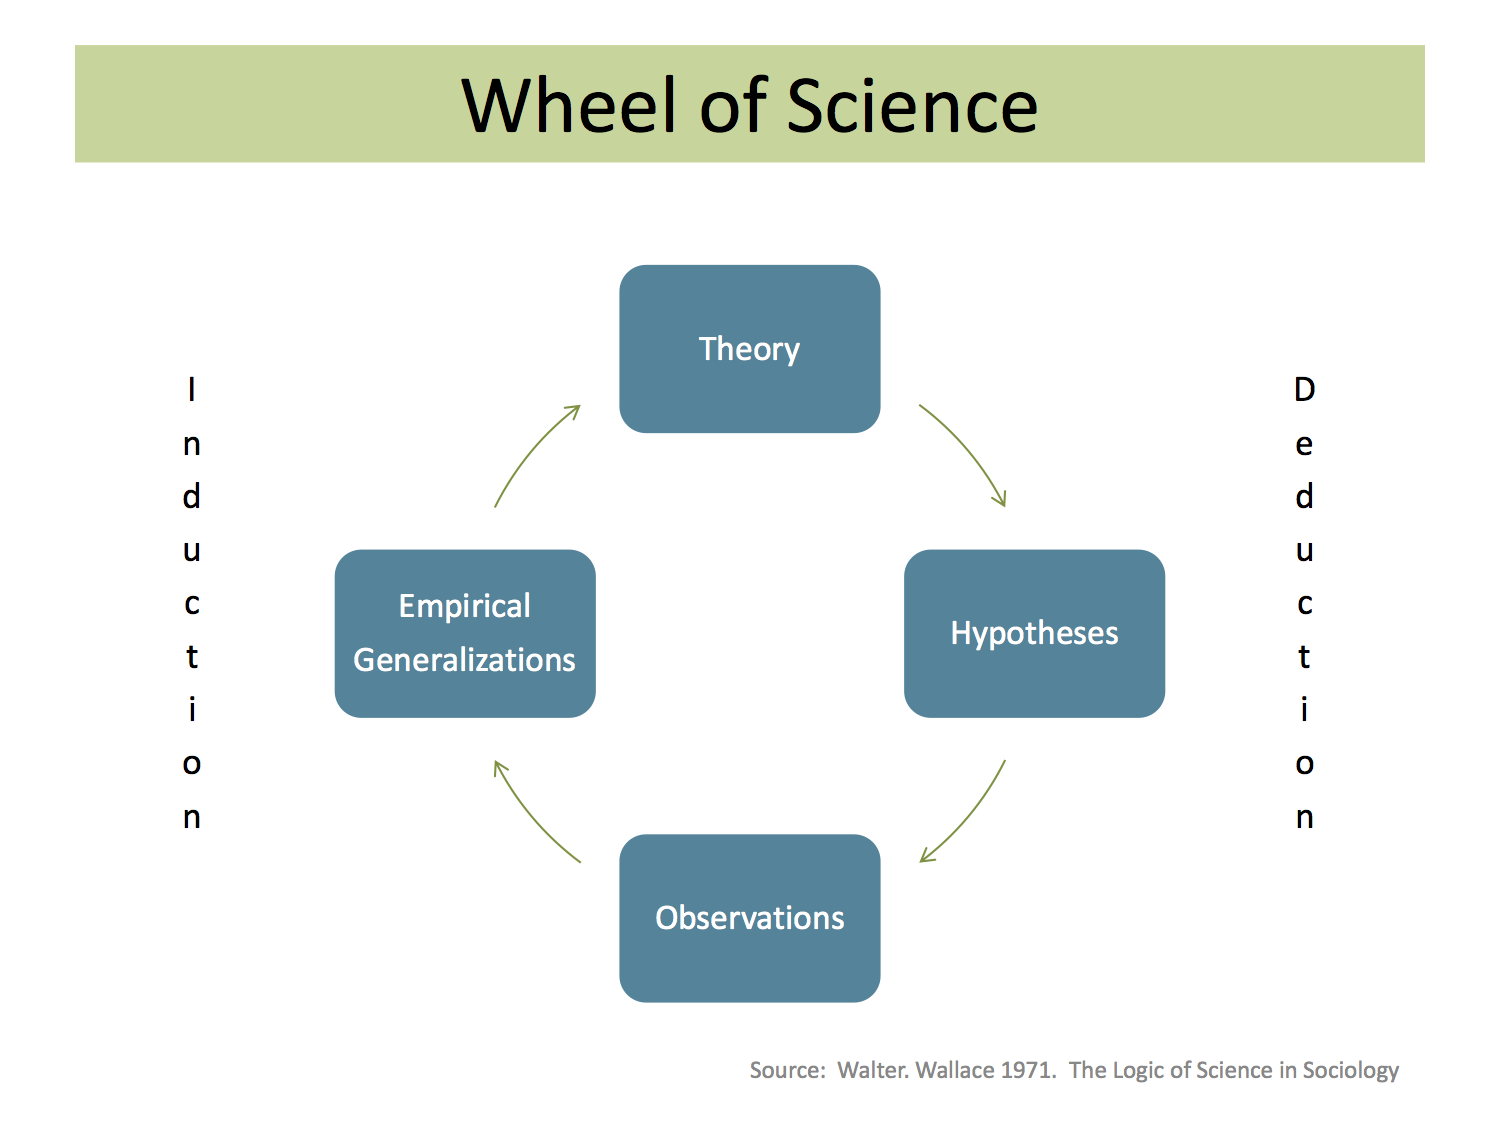
\includegraphics[width=0.45\linewidth]{chapters/Chapter_1/ext_figure/zWheel_Science.png} % requires the graphicx package

   \caption{The Wheel of Science}
   \label{fig:WS}
\end{figure}

\subsection{Example}

Let's look at another example.  Suppose we are interested in comparing the following four popular weight loss diets: Zone (balance between carbohydrates, protein and fat), Atkins (low carbohydrate, high fat, unrestricted calories), LEARN (low fat, based on national guidelines), and Ornish (low fat, high carbohydrate, unrestricted calories).   How would we design a comparison study?

\subsubsection{1.	Conceptualize the problem}

Which weight loss program is most effective?   Which one is the \textit{most healthy}?   Can \\ unrestricted-calorie diets make you lose weight?

\subsubsection{2.	Operationalize the problem}

How would we measure `effective' and `healthy?'  Do we look at weight \textit{loss} after two weeks? Two months?  Two years?  Do we compare the average weight \textit{loss} or percentage of people who lost 15 pounds or more?  How do we measure health?  By cholesterol reduction?  LDL cholesterol reduction?  Blood pressure reduction?  Glucose levels?  Percentage who feel better?

\subsubsection{3.	Design the study}

Where do we recruit our subjects for the study? How long will the study last?  Will we include only overweight subjects?  Do they choose which diet, or do we randomize the selection procedure?  How do we ensure that they stay on the diet?  Do we drop the cheaters from the study?

\subsubsection{4.	Collect the data}

How many times will we measure their weights?  How many times will we take blood samples?  Urine samples?  Do we send all samples to the same lab?  Do we measure how strictly each subject adheres to their diet?

\subsubsection{5.	Analyze the data}

Are there significant differences in average weight loss between diet groups?  Are there significant differences in the percentage who lost weight?  Are there differences in cholesterol changes, blood pressure changes, glucose level changes?  Are there differences in long-term adherence rates to each diet?

\subsubsection{6.	Conclusions}

Which diet would we recommend?  Under what conditions? Are our subjects sufficiently representative to allow generalization?  Are we sure the observed weight loss can be attributed to the diet?

\subsubsection{7.	Disseminate results}

How would we present the results of the study?  What tables and graphs would make the study easy to read and understand?

\subsection{A final product}

The following is a summary of a study reported in the Journal of the American Medical Association (JAMA), Vol. 297, No. 9 in March 2007.  The paper is titled ``Comparison of the Atkins, Zone, Ornish,and LEARN Diets for Change in Weight and Related Risk Factors Among Overweight Premenopausal Women The A TO Z Weight Loss Study: A Randomized Trial,'' by Christopher D. Gardner, PhD, Alexandre Kiazand, MD, Sofiya Alhassan, PhD, Soowon Kim, PhD, Randall S. Stafford, MD, PhD, Raymond R. Balise, PhD, Helena C. Kraemer, PhD, and Abby C. King, PhD.  All authors were affiliated with the Stanford Prevention Research Center and the Department of Medicine, Stanford University Medical School.

\subsubsection{Context}

\textit{Popular diets, particularly those low in carbohydrates, have challenged current recommendations advising a low-fat, high-carbohydrate diet for weight loss. Potential benefits and risks have not been tested adequately.}

\subsubsection{Objective}

\textit{To compare four weight-loss diets representing a spectrum of low to high carbohydrate intake for effects on weight loss and related metabolic variables.  Design, Setting, and Participants Twelve-month randomized trial conducted in the United States from February 2003 to October 2005 among 311 free-living, overweight/obese (body mass index, 27-40) nondiabetic, premenopausal women.  Intervention Participants were randomly assigned to follow the Atkins (n=77), Zone (n = 79), LEARN (n=79), or Ornish (n=76) diets and received weekly instruction for two months, then an additional 10-month follow-up.}

\subsubsection{Main Outcome Measures}

\textit{Weight loss at 12 months was the primary outcome.  Secondary outcomes included lipid profile (low-density lipoprotein, high-density lipoprotein, and non-high-density lipoprotein cholesterol, and triglyceride levels), the percentage of body fat, waist-hip ratio, fasting insulin and glucose levels, and blood pressure. Outcomes were assessed at months 0, 2, 6, and 12. The Tukey studentized range test was used to adjust for multiple testing.}

\subsubsection{Results}

\textit{Weight loss was greater for women in the Atkins diet group compared with the other diet groups at 12 months and mean 12-month weight loss was significantly different between the Atkins and Zone diets $(P<.05)$. Mean 12-month weight loss was as follows: Atkins, -4.7 kg (95\% confidence interval [CI], -6.3 to -3.1 kg), Zone, -1.6 kg (95\% CI, -2.8 to -0.4 kg), LEARN, -2.6 kg (-3.8 to -1.3 kg), and Ornish, -2.2 kg (-3.6 to -0.8 kg). Weight loss was not statistically different among the Zone, LEARN, and Ornish groups. At 12 months, secondary outcomes for the Atkins group were comparable with or more favorable than the other diet groups.}

\subsubsection{Conclusions}

\textit{In this study, premenopausal overweight and obese women assigned to follow the Atkins diet, which had the lowest carbohydrate intake, lost more weight and experienced more favorable overall metabolic effects at 12 months than women assigned to follow the Zone, Ornish, or LEARN diets. While questions remain about long-term effects and mechanisms, a low-carbohydrate, high-protein, high-fat diet may be considered a feasible alternative recommendation for weight loss.}

The study tells us that all three groups lost weight.  Over 12 months, the Atkins group lost the most weight without increasing cholesterol, blood pressure, the percentage of body fat, or fasting glucose levels.

The study does not tell us that if one stays on the Atkins diet long term (say, two years, or five years, or 10 years) their cholesterol, blood pressure, the percentage of body fat, or fasting glucose levels will remain favorable.  If one ‘cheats’ on the Atkins diet periodically, what will be the effect on weight and metabolic profile?  Will the same results be observed for men?  For non-obese women?

Some studies are well designed; others are not.  It is often up to us to make our judgments about what is true, instead of leaving this responsibility to journalists or bloggers.  Whenever you hear a claim on television or in a magazine, ask yourself ``What is the evidence?''

\section{Common Fallacies}

A fallacy is sometimes defined as a mistake in basic reasoning. The following are examples of fallacies:

\begin{enumerate}
\item \textbf{Lack of evidence fallacy}

``There is no proof that the drug is unsafe.''  It allows claims to be made without providing any evidence, simply by shifting the burden of proof.  The fallacy lies in the reasoning that lack of evidence means the contrary is true.

\item \textbf{Anecdotal evidence fallacy}

``We give you testimonies of real people who $\dots$'' improved their golf game, or improved their sex life, or lost weight, or got rid of acne or achieved financial success.  They make claims without comparison studies.  Take a golf infomercial with testimonies from five golfers that a new driver improved their distance and accuracy.  Did it?  These are five golfers out of how many that they approached?  These are televised shots out of how many that each took?  The fallacy lies in the reasoning that existence means prevalence.

\item \textbf{Correlation equals causation fallacy}

For example, ``Married people are happier than singles,''  may be wrongly interpreted as ``Want to be happy? Get married.''  It may be that happy people are the ones who tend to get married, or that high earners tend to be both happy and married.  The fallacy lies in the reasoning that ``two things happening together'' must mean one causes the other.
\end{enumerate}

\subsection{Some fallacies in interpreting evidence} \index{descriptive statistics}

In medical studies, we use clinical trials to see if a difference exists between treatments.  We use statistical analysis to determine if there is a significant difference between the treatment types.  Perhaps there is very little difference, and that difference can be explained as being due to chance.  It could be there is no actual difference between treatment groups.  It leads us to a Type I error which can commonly occur.

A \textbf{Type I error} occurs when the researcher falsely finds a difference between treatments where no actual difference exists.  Often, we use 95\% confidence intervals when analyzing for statistical significance.  It means that 5\% of the time we may conclude a significant difference, when in fact one doesn’t exist!  The researcher is thus willing to accept a 5\% chance that the study conclusions could be wrong.  Notice, however, 5\% is very small compared to the 95\% assurance we have that there is a significant difference.

Another type of error that may be made is a \textbf{Type II error}.  Here the researcher fails to find a difference between the treatment groups when a true difference does exist!  Perhaps we did a study with only a small sample, and we didn't see a difference between our treatment and control group.  We would conclude there is no difference, which the treatment was not effective.  Another lab might perform the same type of study but have a much large sample size, and once they analyze their data find that there is a true difference.  If we fail to find a statistical difference when there is a difference, we have committed a Type II error.  It also relates to the power of a study.  The power of a study is related to the strength of the study.  Can we detect an effect when there is an effect?  How well was the study conducted?  It also relates to our sample size.  When we have a larger sample size, we will reduce the likelihood of committing a Type II error.

\section{Key Words}

\fbox{\parbox{13cm}{
\begin{minipage}[ht]{6cm}

\begin{itemize}
\item correlation
\item data
\item fallacies
\end{itemize}
\end{minipage} \hfill
\begin{minipage}[ht]{6cm}

\begin{itemize}
\item knowledge
\item type I error
\item type II error
\end{itemize}
\end{minipage}
}}



\twocolumn

\section{}    %%%%%%%%%%%%%%%%%%%%%%%%%%%%%%%%%%%%%%%%.

\begin{exercises}
  \begin{exercise}  % 1

  What might be wrong \\ about these headlines?

  \begin{enumerate}
  \item A study proclaims: ``Slightly over- \\ weight people live longer than thin \\ people.''
  \item A study states, ``People who consider themselves depressed eat more chocolate  than people who consider them- \\ selves  otherwise.''
  \item A U.S. Census reported ``More American women are living without a husband than with one.''  Additionally, \\ women rated  themselves happier when \\ compared to the previous year's census.  Can we then infer that living single is leading to greater happiness in women?  What flaw is present here?
  \end{enumerate}

	  % \framebox[5cm][l]{ Answer: }
  \end{exercise}
  \begin{solution}  % 1

1.  What might be wrong about these headlines?
  a.	A study proclaims: ``Slightly overweight people live longer than thin people.'' ``Slightly overweight people live longer than thin people.''  It is a fallacy of correlation equals causation.  It statement implies that being slightly overweight causes people to live longer when compared to thin people.  We would want to dig deeper into the study to see what confounding variables may be present: did we take into account health of the individuals?  Perhaps we have some individuals in poor health leading them to be thin and shortening their lives.

  \end{solution}

   \begin{exercise}  % 2

A handful of people \\ were recently polled on their preference of soda at a local shopping mall in the U.S. and the study indicated more people preferred \\ Mountain Dew over Cola.  It indicates  Mountain Dew is exceeding Cola as the beverage of choice in mainstream America.  What is wrong with this assertion?

  % \framebox[5cm][l]{ Answer: }

  \end{exercise}
  % \begin{solution}  % 2
  %
  % This sample was not random, and it was taken at a local shopping mall somewhere in the U.S.
  % \end{solution}

\begin{exercise}  % 3

A new anti-wrinkle \\ cream was given to several people who frequently purchase make-up products from a specific  company.  In a follow-up with these individuals, all of them assert the new product was highly effective.  What fallacy is \\ present here?  Should the company mass produce this new product? If not, what else \\ needs to be studied here?

% \framebox[5cm][l]{ Answer: }
\end{exercise}
\begin{solution}  % 3

No randomization; the product was given to several people; a skin specialist should make the determination as to the effectiveness of the product; the company should not mass produce this anti-wrinkle cream.

\end{solution}

\begin{exercise}  % 4

All the members (sample \\ size, n=30) of a high school tennis team were given a new racket and were asked to report back on how the racket affected their performance during practices for the week.  All the members of the tennis team then completed a survey, and everyone minus one individual reported that the new racket impacted their performance in a positive manner.  Since we have a large enough sample size can we now conclude the new racket causes tennis players to perform better?  Why or why not?  Is there a fallacy here?

	 % \framebox[5cm][l]{ Answer: }
	\end{exercise}
	 % \begin{solution}  % 4
	 %
	 %
	 % \end{solution}

\begin{exercise}   % 5

Is this advertising claim \\ misleading? 
``More than 8 in 10 Dentists recommend Colgate.''

\end{exercise}
\begin{solution}    % 5

The claim, which was based on surveys of dentists and hygienists carried out by the manufacturer, was found to be misrepresentative as it allowed the participants to select one or more toothpaste brands. The ASA stated that the claim ``… would be understood by readers to mean that 80 percent of dentists recommend Colgate over and above other brands, and the remaining 20 percent would recommend different brands.''

\end{solution}

\begin{exercise}   % 6

You heard a company \\ rumor that the boss was going to crack down on employees who send e-mail from work.  You, recently, read a report that showed most people spend an average of two hours per day checking and sending personal e-mails from work.  You say to yourself `No way do I spend that much time.'  Should this employee be concerned?    

\end{exercise}
\begin{solution}    % 6

\end{solution}



%%%% ADD MORE EXERCISES



\end{exercises}

\onecolumn



%!Rnw root = ../../Main.Rnw

\chapter{Data Presentation}
\label{chap:ch2}

\section{Objectives}

After completing this part, students should be able to:

\fbox{\parbox{14cm}{

\begin{itemize}
\item Recognize the types of variables (categorical or numerical) and give examples of each type.
\item Remember and explain the four levels of measurement and give examples of each level.
\item Tell the difference between dependent and independent variables.
\item Compute the relative frequency.
\item Use graphical methods to display data.
\end{itemize}
}}

\section{Statistics and Data}

\textbf{Statistics} refers to a collection of techniques and procedures for analyzing data.  In this context, statistics may be considered a synonym of data analysis.  In a narrower context, `statistics' is sometimes synonymous with the numbers themselves, such as in `demographic statistics' or `baseball statistics.'  `Data' refers to any collection of measurements that a researcher makes on some number of subjects.  Researchers often store these measurements in a row-and-column display called a spreadsheet.  The following example shows a spreadsheet containing data taken on ten students in a class.

  \begin{table}[htbp]
   \centering
  \begin{tabular}{@{} p{14mm} p{13mm} p{20mm} p{9mm} p{32mm} p{18mm} p{21mm} @{}} \hline % Column formatting, @{} suppresses leading/trailing space
   \multicolumn{7}{c}{CLASS DATA} \\
   %\multicolumn{7}{c}{Class Hours} \\
   Student & Gender & Level & GPA & Credit Hrs Taken & Transport & Hrs Slept \\ \hline
   1 & M & Sophomore & 3.10 & 32 & Car & 7 \\
   2 & M & Junior & 3.20 & 66 & Car & 8 \\
   3 & F & Senior & 3.49 & 94 & Bus & 8 \\
   4 & M & Senior & 2.68 & 89 & Walk & 10 \\
   5 & F & Junior & 3.73 & 69 & Bicycle & 8 \\
   6 & F & Junior & 3.39 & 59 & Car & 8 \\
   7 & F & Senior & 3.80 & 86 & Walk & 8 \\
   8 & M & Junior & 3.11 & 75 & Car & 8 \\
   9 & F & Sophomore & 3.10 & 27 & Car & 7 \\
   10 & M & Senior & 3.10 & 96 & Walk & 3 \\ \hline
   \end{tabular}
   \end{table}

Each row represents a subject (or student, in this case), and each column represents a measurement.  The measurement columns are also called variables because the values vary from one subject to another.

\section{Classification of variables}

\subsection{Levels of Measurement}

It is useful to distinguish between \textbf{four levels of measurements} for variables, from weakest to strongest: Nominal (no ordering), Ordinal (ordering exists, but not distance), Interval (distance exists, but not ratios), and Ratio (ratios exist).

\begin{enumerate}
\item \textbf{Nominal Variables}

Nominal variables are \textbf{categorical variables} that have two or more categories without having any logical sequence or order. For example, Gender is a nominal variable, since `Male' and `Female' are just names of categories.  Additional nominal variable examples include religious affiliation, language, and nationality.   There is no intrinsic ordering between these.  We often use bar charts and pie charts to represent these data.

\fbox{\parbox{14cm}{
\begin{itemize}
\item You cannot perform arithmetic operations like addition, subtraction, \\ multiplication, etc.
\item No order or logical sequence is present
\item Only names
\end{itemize}
}}

\item \textbf{Ordinal Variables}

Ordinal variables are \textbf{categorical variables} with a clear ordering or rank.  A student's level of standing (freshman, sophomore, junior, or senior) is ordinal; they are also names of categories but, unlike gender, they are rank-ordered.   However, we cannot subtract them, and distances do not make sense.  Other examples of ordinal variables include Likert scale items in which we rank items.  Completing surveys or even end of semester evaluations we can rank on a scale of 1-5 (often from strongly disagree to agree strongly).

\fbox{\parbox{14cm}{
\begin{itemize}
\item Be careful about the size of the difference between categories may not be equally spaced.
\item Only order matters not the difference between categories
\end{itemize}
}}

\item \textbf{Interval Variables}

Interval variables are \textbf{numerical variables} where the difference between the two values is meaningful.  GPA is an interval measurement; we can subtract these measurements, and distances make sense.  For example, the distance from 2.3-2.4 is the same distance as 3.7-3.8.  However, ratios do not make sense; is 4.0 `twice as high' as 2.0?  The answer is no.  The grading system would work just as well on the scale (A, B, C)=(5.0, 4.0, 3.0) instead of (4.0, 3.0, 2.0).

\item \textbf{Ratio Variables}

Ratio variables are \text{numerical variables} with true zero.  Number of credit hours is a ratio measurement.  A student who has completed 90 credit hours has twice as many as 45 credit hours and three times as many as 30 credit hours.  Another example is the speed of an automobile which has true zero mph when it is not moving.  A speed of 40 mph is twice as fast as 20 mph.
\end{enumerate}

It is useful to recognize a hierarchy of information in the sense that \textit{a measurement level contains an amount of information greater than or equal to the level below it}.  At lower levels of measurement, data analyses tend to be less sensitive and sophisticated.  A statistical study should aim for the highest levels of measurement possible or affordable.

\subsection{Numerical versus categorical variables}

Interval and ratio variables together are often called \textbf{numerical} variables or \textbf{quantitative} because they provide a number which measures `quantity' (how much, how many) of something.

Nominal and ordinal variables together are often called \textbf{categorical} variables because they classify rather than count or measure.  It is tempting to think of categorical variables as `non-numerical,' but sometimes they do consist of numbers.  For example, `Social Security number' consists of numbers, but are used more as labels rather than quantities.  Hence, SS number is categorical.

\begin{figure}[htbp]
   \centering

   \caption{Mind map of a Random Variable}

   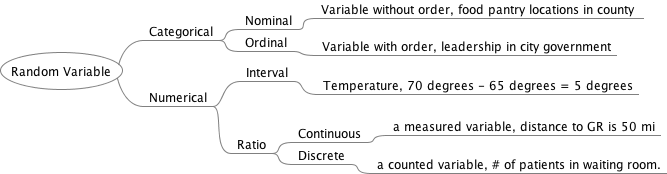
\includegraphics[width=12cm, height=6cm]{chapters/Chapter_2/ext_figure/zRV1.png} % requires the graphicx package
   %{chapters/Chapter_2/ext_figure/varType.png} % requires the graphicx package

\end{figure}


\subsection{Dependent versus independent variables}

Another classification for variables is dependent and independent. This distinction is relevant in studies that investigate cause and effect.  The independent variable is the probable cause.  We also refer to this as the predictor or explanatory variable.  The dependent variable is the outcome variable that is affected by the independent variable.

\fbox{\parbox{14cm}{
In cause-and-effect studies:
\begin{itemize}
\item The \textbf{independent} variable is the probable cause.
\item The \textbf{dependent} variable is the outcome being caused/affected.
\end{itemize}
}}

The following is a description of a clinical study on the possible link between vaccines and autism.   In particular, the study tries to find an association between the amount of a mercury-containing preservative in vaccines and measures of brain function in children.   It has one independent variable (amount of mercury in vaccines) and 42 dependent variables (measures of brain function).  Similar to two previously published studies, it found no evidence of neurologic problems in children exposed to mercury-containing vaccines. \citep{thompson2007}
%The paper is titled ``Early Thimerosal Exposure and Neuropsychological Outcomes at 7 to 10 Years'' by William W. Thompson et al. (New England Journal of Medicine, 2007 Sept; Vol. 357, pp.1281-92).

%\subsubsection{Background}
\begin{enumerate}

\item \textbf{Background}

Others have hypothesized that early exposure to thimerosal, a mercury-containing a preservative used in vaccines and immune globulin preparations are associated with neuropsychological deficits in children.

%\subsubsection{Methods}
\item \textbf{Methods}

William W. Thompson enrolled 1047 children between the ages of seven and ten years and administered standardized tests assessing 42 neuropsychological outcomes. We did not assess autism-spectrum disorders. We determined exposure to mercury from thimerosal from computerized immunization records, medical records, personal immunization records, and parent interviews.  We obtained the information on potential confounding factors from the interviews and medical charts. We assessed the association between current neuropsychological performance and exposure to mercury during the prenatal period, the neonatal period (birth to 28 days), and the first seven months of life.

%\subsubsection{Conclusion}
\item \textbf{Conclusion}

Our study does not support a causal association between early exposure to mercury from thimerosal-containing vaccines and immune globulins and deficits in neuropsychological functioning at the age of 7 to 10 years.
\end{enumerate}

Among the 42 variables used to measure brain function tests on speech and language (comprehension of instructions, recalling sentences, stuttering), tests on verbal memory (no delay, short delay, long delay), tests on motor coordination (grooved pegboard, finger tapping), tests on behavior regulation (hyperactivity, inattentiveness), presence of tics (motor and phonics) and tests on intelligence (verbal IQ, full-scale IQ).  Most of these are numerical test scores.  Others are categorical, like the presence of stuttering (Yes-No) and tics (Yes-No).

Note that the researcher has a choice of whether to use numerical or categorical measures of brain function.  Even for categorical outcomes, there is a choice between nominal (i.e., Yes-No), or ordinal (Frequently-Sometimes-Never). Many surveys like to use the ordinal five-point scale:

{\small{
\begin{enumerate}
\item Strongly agree
\item Agree
\item Neither agree nor disagree
\item Disagree
\item Strongly disagree
\end{enumerate}
}}

It is called a \textit{Likert item}.  The scores from adding up several Likert items is said to be on a \textit{Likert scale}.  Western Michigan University's course evaluation uses a Likert scale on some topics.

\section{Summarizing Categorical Data}

The Census Bureau conducts a separate nationwide survey on population and information.  Called the American Community Survey (ACS), it is ``designed to provide communities a fresh look at how they are changing.'' The ACS collects population and housing information every year instead of every ten years.  The following data is a sample of the actual responses to the ACS from the state of Michigan and Indiana in 2008.

The variables `State' and `Type of Payment' are categorical.  The variables `No. of bedrooms,' `Monthly Payment' and `12-month Household Income' are numerical.


% Requires the booktabs if the memoir class is not being used
\begin{table}[htbp]
   \centering
   %\topcaption{Table captions are better up top} % requires the topcapt package
   % \begin{tabular}{@{} llllll @{}} \hline % Column formatting, @{} suppresses leading/trailing space
   \begin{tabular}{@{} p{2cm} p{2cm} p{2cm} p{2cm} p{2cm} p{2cm} @{}} \hline
      % \toprule
      \multicolumn{6}{c}{Michigan and Indiana ACS Data} \\
      \multicolumn{6}{c}{A Partial List} \\
          &       &           &           &         & 12-month \\
          &       & No. of    & Monthly   & Type of & Household \\
Household &	State	& Bedrooms	& Payment	& Payment 	& Income \\ \hline

1	& Michigan	& 2	& 880	& Rent	& 11200 \\
2	& Michigan	& 3	& 990	& Mortgage	& 80800 \\
3	& Michigan	& 4	& 750	& Mortgage	& 87600 \\
4	& Michigan	& 3	& 1400 &	Mortgage &	94000 \\
5	& Michigan	& 4	& 1400 &	Mortgage &	97000 \\
6	& Michigan	& 1	& 560	& Rent	& 6000 \\
7	& Michigan	& 4	& 900	& Mortgage &	95000 \\
8	& Michigan	& 2	& 0	& None	& 39000 \\
9	& Michigan	& 1	& 380	& Rent	& 24370 \\
10	& Michigan & 2 &	910	& Rent &	54500 \\
$\vdots$ & & & $\vdots$ & &  $\vdots$ \\
39	& Indiana	& 2	& 200	& Mortgage	& 46000 \\
59	& Indiana	& 4	& 200	& Mortgage	& 38300 \\
66  &	Indiana	& 2	& 190	& Mortgage	& 18320 \\
$\vdots$ & & & $\vdots$ & &  $\vdots$ \\
\hline
   \end{tabular}
   \caption{Partial List of Michigan and Indiana ACS Data.}
   \label{tab:booktabs}
\end{table}

\subsection{Relative Frequency Table}

A \textit{relative frequency table} gives the count for each category and the relative frequency or percentage of time in which each category occurs.  Here is a relative frequency table for Monthly Payment type.

% latex table generated in R 4.0.2 by xtable 1.8-4 package
% Fri Jul 31 12:47:10 2020
\begin{table}[ht]
\centering
\begin{tabular}{rrr}
  \hline
 & Frequency & Relative Frequency(\%) \\ 
  \hline
Mortgage & 44 & 58 \\ 
  None & 12 & 16 \\ 
  Rent & 20 & 26 \\ 
  Total & 76 & 100 \\ 
   \hline
\end{tabular}
\caption{Relative Frequency Table for Type of Monthly Payment} 
\end{table}


To compute Relative Frequency, divide Frequency by the total and multiply by 100\%.  For example,

\begin{equation*}
RF(Mortgage) = \frac{\text{Mortgage Frequency}}{\text{Total Frequency}} = \frac{44}{76} \times 100 = 57.9
\end{equation*}

\subsection{Pie Chart}

A pie chart gives the same information as a bar chart, except in a circular shape.  We also use pie charts for categorical data. Some people prefer the look of pie charts over bar charts.  However, studies have shown that people have difficulty comparing the relative size of wedges.  When using this type of chart, we should only consider it when the number of variables is less than six, and we will use bar charts when we have more than six.  Look at the pie chart below.  Is Rent less than half or more than half of Mortgage?



{\centering \includegraphics[width=10cm,height=10cm]{figure/LBL2c-1} 

}





\newpage

\subsection{Bar Chart}

A \textit{bar chart} is a plot of the relative frequency table.  We use bar charts for categorical data. The order by which the categories are presented in the bar chart is arbitrary. Sometimes they are presented in order of decreasing frequency for aesthetic purposes and is called a Pareto chart.  Some computing packages present the categories alphabetically unless otherwise specified.



{\centering \includegraphics[width=8.0cm,height=7cm]{figure/LBL2b-1} 

}





\section{Summarizing numerical data}

Remember that the	\textit{mean} and \textit{median} cannot be used for nominal variables.

Consider the variable Monthly Payment in the ACS housing data on page 26.  How do the numbers appear?  How large are they? How variable is the data?  Are there any extreme values? These questions are attempts at getting to know the data.  In this section, we discuss tools for getting to know numerical data better.  We have n = 64 observations available since 12 households (out of 76) do not have monthly payments.  Here is a list of the monthly payments:

{\small{
880, 990, 750, 1400, 1400, 560, 900, 0, 380, 910, 1200, 1200, 450, 1200, 1300, 550, 340, 770, 700, 700, 0, 0, 0, 140, 220, 0, 650, 5200, 0, 970, 740, 500, 700, 1800, 800, 1200, 1000, 1200, 200, 710, 1100, 400, 370, 670, 350, 510, 0, 900, 0, 340, 440, 1500, 0, 420, 490, 2400, 0, 500, 200, 670, 760, 720, 0, 500, 280, 190, 1000, 250, 700, 380, 740, 0, 850, 530, 290, 230
}}

Now, we sort the observations from smallest to largest:

{\small{
140, 190, 200, 200, 220, 230, 250, 280, 290, 340, 340, 350, 370, 380, 380, 400, 420, 440, 450, 490, 500, 500, 500, 510, 530, 550, 560, 650, 670, 670, 700, 700, 700, 700, 710, 720, 740, 740, 750, 760, 770, 800, 850, 880, 900, 900, 910, 970, 990, 1000, 1000, 1100, 1200, 1200, 1200, 1200, 1200, 1300, 1400, 1400, 1500, 1800, 2400, 5200
}}

The smallest observation is \$140.  The largest is \$5200, which is an \textbf{outlier}.

\fbox{\parbox{14cm}{In data analysis, an \textbf{outlier} is an observation that falls far from the rest of the data. It may need to be checked for correctness if there is any possibility of clerical error.}}

Can this be a typographical error that we need to correct?  When we Look closely at the data, we see it belongs to observation 28, which is a mortgage for a household with a \$358,000 annual income.  We can infer that it is probably correct, so we leave it alone. The simple act of sorting the data already gives us more information about monthly payment.  For example, we can now see that the typical monthly payment falls around \$700.  We also see the extent to which the \$5200 value is outlying. We now turn to better ways to visualize the \textbf{spread} of this data.

\subsection{Stem-and-Leaf Plot}




Graphs are helpful in summarizing information in the data, especially for large datasets.  Below, we summarize two-year average percentage of persons living in poverty (2008-2009) in the U.S.A. in a graph called a stem-and-leaf plot.  The numbers on the left are stems, while the numbers on the right are called leaves.

%  \newpage

\begin{minipage}[ht]{7cm}

{\small{


7.4, 8.2, 8.6, 9.1, 9.2, 9.3, 9.7, 9.9, 10.1, 10.2, 10.3, 10.5, 10.5, 10.9, 11, 11, 11.1, 11.2, 11.4, 11.7, 11.7, 11.9, 12, 12.8, 12.9, 13, 13.2, 13.2, 13.3, 13.5, 13.5, 13.6, 13.9, 13.9, 14.4, 15, 15, 15.2, 15.2, 15.4, 15.4, 15.8, 16.2, 16.6, 16.9, 17, 17.1, 17.2, 19.3, 19.6, 20.6
}}
\end{minipage} % \hfill
\begin{minipage}[ht]{7cm}

{\small{
\begin{verbatim}

  The decimal point is at the |

   7 | 4
   8 | 26
   9 | 12379
  10 | 123559
  11 | 00124779
  12 | 089
  13 | 022355699
  14 | 4
  15 | 0022448
  16 | 269
  17 | 012
  18 | 
  19 | 36
  20 | 6


\end{verbatim}
}}
\end{minipage}

There is one leaf for each observation, so there are 51 leaves in all, one for each state.  Our smallest observation is 7.4.  We write it on the stem `7' as a leaf of `4.'  We can infer that the stems represent tens and units digits while the leaves represent tenths digits.  We write the value 20.6 on the stem `20' as a `20' and the leaf as a `6', and so forth.  \citep{sullivan2013}

% Suppose we want to compare mortgage and rent.  Do mortgage payments tend to be greater or less than rent?  We can present stem-and-leaf for mortgage and rent side by side.
%
% %  \newpage
%
% Stem and Leaf Display of Monthly Payment (stem width \$100)
%
% \begin{center}
%
% {\footnotesize{
% \begin{minipage}[ht]{3cm}
%
% Mortgage
%
% \begin{tabular}{@{} r|l @{}} \hline
% 1 & 9 \\
% 2 & 0039 \\
% 3 & 478 \\
% 4 & 245 \\
% 5 & 00135 \\
% 6 & 7 \\
% 7 & 0012457 \\
% 8 & 05 \\
% 9 & 007 \\
% 10& 00 \\
% 11& 0 \\
% 12& 0000 \\
% 13& 0 \\
% 14& 00 \\
% 15& 0 \\
% 16& \\ \hline
% \end{tabular}
% \end{minipage}
% \begin{minipage}[ht]{4cm}
%
% Rent
%
% \begin{tabular}{@{} r|l @{}} \hline
% 1 & 4 \\
% 2 & 258 \\
% 3 & 458 \\
% 4 & 09 \\
% 5 & 06 \\
% 6 & 57 \\
% 7 & 0046 \\
% 8 & 8 \\
% 9 & 1 \\
% 10&  \\
% 11&  \\
% 12& 0 \\
% 13&  \\
% 14&  \\
% 15&  \\
% 16& \\ \hline
% \end{tabular}
% \end{minipage}
% }}
% \end{center}
%
% In general, rent is smaller than mortgages and less variable.  While mortgages seem centered around \$700, rent is centered around \$500.  Furthermore, mortgages have a longer right tail, with a significant percentage over \$1000.  Plus, remember that we have removed a \$1800 - \$5200 mortgages from these plots.

\subsection{Relative Frequency Table and Histogram}

Earlier in this chapter, we presented a relative frequency table for categorical data.  Relative frequency tables may also be used for numerical data.  A relative frequency table for monthly payment is presented below.  The class width is chosen to achieve a moderate number of class intervals.

{\small{
% latex table generated in R 4.0.2 by xtable 1.8-4 package
% Fri Jul 31 12:47:10 2020
\begin{table}[ht]
\centering
\begin{tabular}{rrr}
  \hline
 & Frequency & Relative Frequency(\%) \\ 
  \hline
0-200 & 2 & 3 \\ 
  200-400 & 13 & 20 \\ 
  400-600 & 12 & 19 \\ 
  600-800 & 14 & 22 \\ 
  800-1000 & 8 & 12 \\ 
  1000-1200 & 3 & 5 \\ 
  1200-1400 & 6 & 9 \\ 
  1400-1600 & 3 & 5 \\ 
  1600-1800 & 1 & 2 \\ 
  2400-2600 & 1 & 2 \\ 
  5200-5400 & 1 & 2 \\ 
   \hline
\end{tabular}
\caption{RF Table of Monthly Payment for ACS Housing Data} 
\end{table}

}}

There are three things to keep in mind when constructing a frequency table. First, decide how many classes (i.e., intervals) we want.  This also determines the \textit{class width}.  Try to have 5 to 15 intervals, depending on how many observations we have. Second, decide where the first interval starts.  Third, decide how to avoid boundary disputes.

The last item requires us to choose a \textbf{boundary convention}.  For instance, the intervals in the frequency table above could have been written as follows:

\vspace{3mm}

\begin{minipage}[ht]{6cm}

\begin{tabular}{@{} l @{}} \hline
0-199 \\
200-399 \\
400-599 \\
600-799 \\
etc. \\ \hline
\end{tabular}

\end{minipage}
\begin{minipage}[ht]{6cm}

\begin{tabular}{@{} l @{}} \hline
$ [0-200)$ \\
$ [200-400)$ \\
$ [400-600)$ \\
$ [600-800)$ \\
 etc. \\ \hline
\end{tabular}
\end{minipage}

\vspace{3mm}

This way, it is easier to tell that \$200 belongs to the second interval, not the first.  However, the table looks more complicated, harder to read.  To keep the intervals simple but avoid boundary disputes, include a footnote to the table that describes the boundary convention, i.e. ``Intervals contain the left endpoint but not the right.''  Then, we know that \$200 belongs to the second interval, not the first.  Alternatively, we may use square braces and parenthesis.

It also means that the class intervals contain the left endpoint but not the right.  Which method do we prefer?

The relative frequency table is a compact numerical way to present how the data is distributed.  If we plot the frequencies as columns, the resulting plot is called a \textit{histogram}.

The histogram and stem-and-leaf plots look alike, except that the stem-and-leaf plot has columns that go sideways instead of upwards.  Stem-and-leafs are better if we want the data values themselves available from the plot.  However, the histogram can handle large sample sizes easily and is more flexible in choosing class widths.  For example, we may choose class widths of \$500, as follows: $[0,500), [500,1000), [1000,1500), \dots, [5000,5500)$, which stem plots cannot do.

% \newpage

\begin{figure}[ht]

\caption{Monthly Payments }



{\centering \includegraphics[width=7cm,height=7cm]{figure/LBL2g-1} 

}




\end{figure}

\subsection{Dot Plot}

For moderately large samples, a \textit{dotplot} diagram is a quick way to see repeating data values.  We present the dot-plots of the resting pulse rates among college students before and after exercise.  As we observed using side-by-side dots plots, we find that the after exercise spread (maximum minus minimum) is wider than before exercise which makes sense.  We also see that six students of the 28 had a pulse rate of 68 beats per minute.

\begin{figure}[ht]

\caption{Dot Plot }



{\centering \includegraphics[width=10cm,height=5cm]{figure/LBL2h-1} 

}




\end{figure}

\newpage

\subsection{Box-and-Whisker Plot}

A box-and-whisker or boxplot shows useful information about the data including the measures the central tendency and the variability of the distribution.  First, order the data from smallest to largest.  What is the range of the first (or smaller) half of the data?  The smallest quarter of the data?  The next quarter?  The box-and-whisker plot or boxplot is a graphical picture of the distribution of quarters of the data.  Consider once again the monthly payments from the ACS housing data.  We list them here sorted from smallest to largest (minus the outlier  (\$5200)).


{\small{
140, 190, 200, 200, 220, 230, 250, 280, 290, 340, 340, 350, 370, 380, 380, 400, 420, 440, 450, 490, 500, 500, 500, 510, 530, 550, 560, 650, 670, 670, 700, 700, 700, 700, 710, 720, 740, 740, 750, 760, 770, 800, 850, 880, 900, 900, 910, 970, 990, 1000, 1000, 1100, 1200, 1200, 1200, 1200, 1200, 1300, 1400, 1400, 1500, 1800, 2400
}}
     %  {\small{
     %  140  190  200  200  220  230  250  280  290  340  340  350  370  380  380
     %  400  420  440  450  490  500  500  500  510  530  550  560  650  670  670
     %  700  700  700  700  710  720  740  740  750  760  770  800  850  880  900
     %  900  910  970  990 1000 1000 1100 1200 1200 1200 1200 1200 1300 1400 1400
     % 1500 1800 2400
     %  }}

There are $n = 63$ observations.  One-quarter of the data is 63/4=15.75, or approximately 16 observations.  The boxplot below gives the range of each quarter of the data: the range of the first quarter (i.e., the lowest 16 monthly payments) is the left whisker.  The range of the 2nd quarter is the left part of the box, the 3rd quarter the right part of the box, and the range of the last quarter is the right whisker.

\begin{figure}[ht]

\caption{Box Plot }



{\centering \includegraphics[width=7cm,height=7cm]{figure/LBL2i-1} 

}




\end{figure}

More precisely, the software draws vertical lines at (140, 400, 700, 970, 2400).  Hence, the lowest 16 monthly payments lie within (\$140, \$400).  The next set of 16 observations lies within (\$400, \$700).  The third set lies within (\$700, \$970).  Finally, the last 16 observations lie within (\$970, \$2400).  The five values (140, 400, 700, 970, 2400) that divide the data into quarters and form the fences and whiskers of the boxplot are collectively called the five-number-summary of the data.  They are often denoted as MIN, $Q_1$, MED, $Q_3$, and MAX respectively.

\newpage

{\small{
\begin{enumerate}
\item	\textbf{MIN} is called the \textbf{minimum} and is the smallest of the ordered observations.
\item	\textbf{$Q_1$} is the median of the lower half of the data.  Also, the is the upper boundary of the first quarter and is called the \textbf{first quartile}.
\item	\textbf{MED} is the upper boundary of the second quarter and is called the \textbf{second quartile}.  However, it also divides the data into lower and upper halves and is more often called the median.
\item	\textbf{$Q_3$} is the median of the upper half of the data.  Also, it is the upper boundary of the third quarter and is called the \textbf{third quartile}.
\item	\textbf{MAX} is the largest of the ordered observations and is called the \textbf{maximum}.
\end{enumerate}
}}

Boxplots are particularly useful for comparing two distributions side-by-side.  Below are boxplots of mortgage data and rent drew parallel to each other on the same scale.  When comparing data of mortgages and rental, we find that mortgages tend to be larger than rent since the median and quartiles are larger.  There is also a considerable difference in the spread, with the mortgage data having a long right tail, evidence that mortgages have a higher ceiling than rent.

\begin{figure}[ht]

\caption{Box Plot }



{\centering \includegraphics[width=8cm,height=8cm]{figure/LBL2j-1} 

}




\end{figure}

\newpage 

Different statistical computing packages have different ways of computing the quartiles, but the differences are minimal.  In this class, we compute the quartiles as follows.  First, arrange the observations from smallest (1st ordered observation) to largest ($n^{th}$ ordered observation).  Then

\fbox{\parbox{14.5cm}{
$Q_1$ is the .25(n+1)th ordered observation. \newline
MED is the .50(n+1)th ordered observation. In other words, the median is the middle value or the average of the two middle values \newline
$Q_3$ is the .75(n+1)th ordered observation.
}}

If .25(n+1) is not an integer, take the average of the two adjacent ordered observations.  Similarly, for MED and $Q_3$.  Here again are the $n = 63$ ordered observations of monthly payments.

{\small{
140, 190, 200, 200, 220, 230, 250, 280, 290, 340, 340, 350, 370, 380, 380, 400, 420, 440, 450, 490, 500, 500, 500, 510, 530, 550, 560, 650, 670, 670, 700, 700, 700, 700, 710, 720, 740, 740, 750, 760, 770, 800, 850, 880, 900, 900, 910, 970, 990, 1000, 1000, 1100, 1200, 1200, 1200, 1200, 1200, 1300, 1400, 1400, 1500, 1800, 2400
}}
% {\small{
% 140  190  200  200  220  230  250  280  290  340  340  350  370  380  380
%       400  420  440  450  490  500  500  500  510  530  550  560  650  670  670
%       700  700  700  700  710  720  740  740  750  760  770  800  850  880  900
%       900  910  970  990 1000 1000 1100 1200 1200 1200 1200 1200 1300 1400 1400
%      1500 1800 2400
% }}


Since .25(63+1)=16, then $Q_1$ is the $16^{th}$ ordered observation.  Hence $Q_1 = 400$.  Similarly, \\ 0.50(63+1)=32 so MED=700.  Finally, .75(63+1)=48, so $Q_3 = 970$.

If $n = 64$, then .25(64+1) = 16.25, so that $Q_1$ would be the average of the $16^{th}$ and $17^{th}$ ordered observations.  Therefore, if we return the \$5200 outlier we removed, then the five-number-summary would be (140, 410, 700, 980, 5200).

\subsection{Symmetry and Skewness}

The shape of the data is often described by its symmetry or non-symmetry (also called skewness).  Here are stem-and-leaf plots for \textit{symmetric}, \textit{right skewed}, and \textit{left-skewed} data.

\vspace{3mm}

\begin{minipage}[ht]{4.5cm}

Symmetric Data



\begin{tabular}{@{} r|l @{}} \hline
4 & 7 \\
5 & 35 \\
6 & 115 \\
7 & 11112 \\
8 & 467899 \\
9 & 1199 \\
10 & 14 \\
11 & 1 \\ \hline
\end{tabular}
\end{minipage}
\begin{minipage}[ht]{4.5cm}

Right-Skewed Data



\begin{tabular}{@{} r|l @{}} \hline
4 & 58 \\
5 & 112345569 \\
6 & 2445 \\
7 & 17 \\
8 & 5 \\
9 & 2 \\
10 & 5 \\
11 & 2 \\ \hline
\end{tabular}
\end{minipage}
\begin{minipage}[ht]{4.5cm}

Left-Skewed Data




\begin{tabular}{@{} r|l} \hline
4 & 0 \\
5 & 5 \\
6 & 2 \\
7 & 5\\
8 & 17 \\
9 & 2445 \\
10 & 111245569 \\
11 & 58 \\ \hline
\end{tabular}
\end{minipage}

\vspace{1cm}

The term `skew' refers to the direction of the most extended tail when you flip the stem-and-leaf sideways or draw a histogram. See histogram examples below. A long tail denotes presence of extreme or outlying observations.  The left-skewed histogram contains observations that are small and outlying, while a right-skewed histogram would have observations that are large and outlying.  A left skew also indicates that the smallest quarter of observations will be more spread out.

% label=LBL2n, results="asis", echo=FALSE, out.width="4cm">>=
%  SDat4 <- c(401,501,601,702,801,802,901,902,903,904,905,1001,1002,1003,1004,1005,1006,1007,1008,1101,1102)
%  hist(SDat4, xlab="values", col="green", main="Left Skewed")
% @
%
% For some further examples of histograms depicting both symmetry and skewness, see below.

\newpage

\begin{figure}[ht]

\begin{knitrout}\footnotesize
\definecolor{shadecolor}{rgb}{0.969, 0.969, 0.969}\color{fgcolor}

{\centering \includegraphics[width=4.5cm,height=4.5cm]{figure/LBL2o-1} 
\includegraphics[width=4.5cm,height=4.5cm]{figure/LBL2o-2} 
\includegraphics[width=4.5cm,height=4.5cm]{figure/LBL2o-3} 

}



\end{knitrout}

\end{figure}

%% \newpage

\section{Key Words}

\fbox{\parbox{14cm}{

\begin{minipage}[ht]{6cm}

\begin{itemize}
  \item data
  \item dependent
  \item graphical methods
    \begin{itemize}
    \item bar chart
    \item box and whisker
    \item dot plot
    \item histogram
    \item pie chart
    \item stem-and-leaf
    \end{itemize}
  \end{itemize}

  \end{minipage}
  \begin{minipage}[ht]{6cm}
  \begin{itemize}
  \item independent
  \item statistics
  \item tabular methods
    \begin{itemize}
    \item relative frequency table
    \end{itemize}
  \item variables
    \begin{itemize}
    \item categorical
    \item numerical
    \end{itemize}

\end{itemize}

\end{minipage}
}}

\section{Summary}

\begin{itemize}
\item	We cannot use the \textit{mean} or \textit{median} for nominal variables.
\item We cannot use the mean for ordinal variables.
\end{itemize}

%%  \newpage

\twocolumn

\section{}

 \begin{exercises}    %%%%%%%%%%%%%%%%%%%%%%%%%%%%%%%%%%%%%%%%%%%%
  \begin{exercise}  % 1

Identify the following \\ types of  data as numerical or categorical.  If numerical, further classify into interval or ratio. If categorical, classify if it is nominal or ordinal.

	  \begin{enumerate}
	  \item The scores on exam one for Stat 1600.
    \item Marital status
    \item Annual income
    \item Social Security Number
    \item Cumulative GPA
    \item Academic level (freshman, sophomore, junior, senior, other)
    \item Quality (poor, fair, good, excellent)
    \item Height (short, average, tall)
    \item Age (years)
    \item Grade $(A, B, C, \dots)$
    \item Color
    \item Rating of eight local plays (poor, fair, good, excellent).
    \item Times required for mechanics to do a tune-up.
  	\end{enumerate}

    % \framebox[5cm][l]{ Answer: }

  \end{exercise}
  \begin{solution}  % 1

    \begin{enumerate}
	  \item   numeric, ratio
    \item  categorical, nominal
    \item  numeric, ratio
    \item  categorical, nominal
    \item  numeric, interval
    \item  categorical, ordinal
    \item  categorical, ordinal
    \item  categorical, ordinal
    \item  numeric: ratio
    \item  categorical, ordinal
    \item  categorical, nominal
    \item  categorical, ordinal
    \item  numeric, interval
  	\end{enumerate}
  \end{solution}

  \begin{exercise} % 2

The 6-year graduation \\ rate for a random sample of 30 colleges and universities
in the U.S. is displayed in the \\ stem-and-leaf plot below.  Note that the stem unit is 10\%, and the leaf unit is 1\%.  For example, the maximum value is 92\%.

\begin{table}[ht]
\centering
{\small{
\begin{tabular}{@{} r|l @{}} \hline
2 & \\
3 & 4 \\
4 & 56889 \\
5 & 01112345567889 \\
6 & 0124457 \\
7 & 17 \\
8 & \\
9 & 2 \\ \hline
\end{tabular}
}}
\end{table}

	  \begin{enumerate}
	  \item Obtain the five-number summary.
    \item Obtain a boxplot and histogram for \\ 6-year graduation rate.
    \item In our opinion, which of the three plots (stem-and-leaf, boxplot, histogram) \\ best illustrates the data? Why?
	  \end{enumerate}

	\end{exercise}
%	\begin{solution}  % 2


%  \end{solution}

  \begin{exercise} % 3

A manager of a car \\ rental company took a random sample of 100 business days over the last fiscal year and \\ recorded the number of cars rented per day.  The frequency distribution of the data is \\ given below.

{\small{
\begin{tabular}{@{} lcc @{}} \hline
Interval  &  Frequency &	Relative Frequency \\
$(20, 25]$ 	&      4 \\
$(25, 30]$ 	&    11  \\
$(30, 35]$ 	&    23 \\
$(35, 40]$ 	&    31 \\
$(40, 45]$ 	&    15 \\
$(45, 50]$ 	&    10 \\
$(50, 55]$ 	&      6 \\ \hline
\end{tabular}  }}

\begin{enumerate}
\item Fill in the relative frequencies above.
\item	Draw a histogram by hand, with either the frequencies or relative frequencies as the vertical axis.
\item	What interval does the median number of car rentals per day fall?
\item What percentage of business days had 30 or fewer car rentals?
\item	How many business days had more \\ than 45 car rentals?
\end{enumerate}

   % \framebox[5cm][l]{ Answer: }

	\end{exercise}
	\begin{solution}  % 3


Compute relative frequencies:

\begin{tabular}{@{} lcc @{}} \hline
Interval  &  Frequency &	Relative Frequency \\
$(20, 25]$ 	&     4 & 4  \\
$(25, 30]$ 	&    11 & 11 \\
$(30, 35]$ 	&    23 & 23 \\
$(35, 40]$ 	&    31 & 31 \\
$(40, 45]$ 	&    15 & 15 \\
$(45, 50]$ 	&    10 & 10 \\
$(50, 55]$ 	&     6 & 6 \\ \hline
\end{tabular}


	\end{solution}

\begin{exercise}  % 4

The following plots represent five different samples of data. For \\ each, describe the shape.

\begin{figure}[ht]
  \caption{Describe Shapes}

\begin{minipage}[ht]{3cm}

  a)

  \includegraphics[width=83pt]{chapters/Chapter_2/ext_figure/boxq7.png}
  \end{minipage} \hfill
  \begin{minipage}[ht]{3cm}

  b)

  \includegraphics[width=83pt]{chapters/Chapter_2/ext_figure/boxq7b.png}
  \end{minipage} \hfill
  \begin{minipage}[ht]{3cm}

  c)

  \includegraphics[width=83pt]{chapters/Chapter_2/ext_figure/boxq7c.png}
  \end{minipage} \hfill
  \begin{minipage}[ht]{3cm}

  d)

    \begin{tabular}{@{} r|l @{}} \hline
  4 & 58 \\
  5 & 011245569 \\
  6 & 2445 \\
  7 & 17 \\
  8 &  \\
  9 & 2 \\
  10 & 5 \\
  11 & 0
    \end{tabular}
  \end{minipage} \hfill
  \begin{minipage}[ht]{3cm}
  e)

  \begin{tabular}{@{} r | l @{}} \hline
  0 & 4 \\
  1 & 889 \\
  2 & 11467 \\
  3 & 457 \\
  4 & 7
  \end{tabular}
  \end{minipage}

\end{figure}

%\framebox[5cm][l]{ Answer: }
\end{exercise}
\begin{solution}  % 4

2.5-7.1: Left-skewed

2.5-7.2: Symmetric

2.5-7.3: Left-skewed

2.5-7.4: Right-skewed

2.5-7.5: Symmetric

\end{solution}

	%%%%%%%%%%%%%%%%%%%%%%%%%%%%%%%% new %%%%%%%%%%%%%%%%%%%%

  \begin{exercise}  % 5

  A survey contained a \\ question regarding marital status.   The \\ respondent checked either single, married,  \\ divorced, separated or widowed.  What is the level of measurement of marital status?
	  \begin{enumerate}
	  \item Ordinal
	  \item Interval-Ratio
	  \item Nominal
	  \item I don't know
	  \end{enumerate}
	  \vspace{3mm}
	  \framebox[5cm][l]{ Answer: }
	\end{exercise}
	\vspace{2mm}
	\begin{solution}
	  The level of measurement of marital status is nominal.
	\end{solution}

  \begin{exercise} % 6

  Blood alcohol content \\ (BAC) is the concentration of alcohol present in a person's blood.  What is the level of measurement of BAC?
	  \begin{enumerate}
	  \samepage
	  \item Ordinal
	  \samepage
  	\item Interval-Ratio
  	\samepage
	  \item Nominal
	  \samepage
	  \item I don't know
	  \samepage
	  \end{enumerate}
	  \samepage
	  \vspace{3mm}
	  \framebox[5cm][l]{ Answer: }
	\end{exercise}
	\vspace{2mm}
	\begin{solution}
	  The level of measurement of marital status is category - nominal.
	\end{solution}

  \begin{exercise}  % 7

  What type of variable \\ is the number of robberies reported in June 2014 in Kalamazoo County?
	  \begin{enumerate}
  	\samepage
  	\item Attribute
  	\samepage
  	\item Discrete
  	\samepage
  	\item Continuous
  	\samepage
  	\item Qualitative
  	\end{enumerate}
  	\vspace{3mm}
  	\framebox[5cm][l]{ Answer: }
  \end{exercise}
  \vspace{2mm}
	\begin{solution}
	
	  The number of reported robberies in June 2014 is Kalamazoo County is a continuous variable.
	  
	\end{solution}

	\begin{exercise}  % 8

	The team of researchers \\ took the following items from a 2007 survey of drug use among young UK children \cite{Teen2007}.  In how many occasions have you \\ used or taken Cannabis?  Determine whether the data are categorical or numerical and the level measurement.

  % \end{minipage} \hfill
  % \begin{minipage}[[htbp]{6.5cm}

{\small{
  \begin{table}[htbp]
   \centering
  \begin{tabular}{@{} rl @{}} \hline % Column formatting, @{} suppresses leading/trailing space
    \underline{ \phantom{xxx} } & Never \\
    \underline{ \phantom{xxx} } & Once \\
    \underline{ \phantom{xxx} } & 2 - 8 occasions \\
    \underline{ \phantom{xxx} } & 9 - 15 occasions \\
    \underline{ \phantom{xxx} } & More than 15 occasions \\ \hline
   \end{tabular}
   \end{table}
}}

  % \end{minipage}
    \vspace{4mm}

    \framebox[5cm][l]{ Answer: }

  \end{exercise}
  \vspace{2mm}
  \begin{solution}   % 8

    Numeric - interval

  \end{solution}

	\begin{exercise}  % 9

	The researchers asked \\ students the following questions from a 2007 survey of drug use among young UK children  \cite{Teen2007}.
	Write the number of glasses of liquors (e.g., Baileys, gin, tequila, vodka) drunk in the last seven days   \underline{\phantom{xxxx}}.
	 Determine whether they are categorical or numerical \\ and the level of measurement.

    \vspace{4mm}

    \framebox[5cm][l]{ Answer: }

  \end{exercise}
  \vspace{2mm}
  \begin{solution}   % 9

    Numeric  ratio

  \end{solution}

% % \pagebreak
% %
	\begin{exercise}  % 10

	  The General Social \\ Survey (GSS), conducted by the National \\ Opinion Research Center at the University of Chicago, is a primary source of data on social attitudes in the U.S.  Once each year, researchers from UC interview 1500 adults in their homes all across the country.  They ask subjects their opinions about sex and marriage, attitudes toward women, welfare, foreign policy, and many other issues \cite{GSS2014}.

    The population for the GSS is
    \begin{enumerate}
    \item the 1500 persons interviewed.
    \item the University of Chicago.
    \item the list of questions asked.
    \item all adult residents of the U.S.
    \end{enumerate}
    \vspace{3mm}
    \framebox[5cm][l]{ Answer: }

  \end{exercise}
  \vspace{2mm}
  \begin{solution}   % 10

    all adult residents of the U.S.
  \end{solution}

\begin{exercise}  % 11

	  A recent issue of the \\ \emph{New England Journal of Medicine} reported a study of all 122,754 infants born over an 8.5 year period at Parkland Hospital in Dallas, Texas, leaving out multiple births and babies with birth defects.  The researchers  wanted to \\ know if there is a specific birth weight below which infant death and illness increases sharply.

    The independent variable in the study is
    \begin{enumerate}
    \samepage
    \item death and illness.
    \samepage
    \item infants (leaving out multiple births, \\ etc.)
    \samepage
    \item birth weight.
    \samepage
    \item Parkland Hospital.
    \end{enumerate}
    \samepage
    \vspace{3mm}
    \framebox[5cm][l]{ Answer: }

  \end{exercise}
  \vspace{2mm}
  \begin{solution}
    birth weight.
  \end{solution}

\begin{exercise}  % 12

  For the following \\ research project, classify all variables in \\ terms of levels of measurement and reveal whether  they're continuous and discrete.  As \\ researchers, we should select the correct statistical method: {\emph{single variable descriptive}}  \\ {\emph{statistic}} or {\emph{a multi-variable descriptive  statistic}} or  {\emph{inferential statistics.}}  Recall that it is common for some projects to require more than one type of method.

	  Ten years ago, a state re-instituted the execution for first-degree murder.  Researchers asked, did this change of policy reduce capital crime?  A team of researchers gathered data on the number of homicides in the state for two-year periods before and after the policy change.

    \vspace{3mm}
    \framebox[5cm][l]{ Answer: }

  \end{exercise}
  \vspace{2mm}
%   \begin{solution}  %12
%
%     Variable: Homicide rate \\
%     Level of Measurement: Interval-ratio \\
%     Type: Continuous \\
%     Application: Descriptive (two variables)
%
%   \end{solution}
%
\begin{exercise}   % 13

The enrolled \\ student population  at Western  Michigan  \\ University (spring 2020) is displayed in the  following table:

{\footnotesize{
  \begin{table}[htbp]
   \centering
  \begin{tabular}{@{} lc @{}} \hline % Column formatting, @{} suppresses leading/trailing space
    Ethnicity & Percent \\ \hline
    American Indian  & 0.433  \\
    Asian & 2.16 \\
    Black  & 11.2 \\
    Hispanic or Latino & 5.61 \\
    Native Hawaiian & 0.0831 \\
    Two or More Races & 3.44 \\
    White & 68.7 \\ \hline
   \end{tabular}
   \end{table}
}}

Draw a histogram by hand of the percentages with the correct labels.

\end{exercise}






% 	\begin{exercise}  % 13
%
% 	  For the following research project, classify all variables regarding levels of measurement and reveal whether they're continuous and discrete.  We should also \\ select which statistical method should be \\ used: {\emph{single variable descriptive statistic}} or \\ {\emph{a multi-variable descriptive statistic}} or \\ {\emph{inferential statistics}}.  Recall that it is \\ common for some projects to require more than one type of method.
%
% 	  Our relative is running for a seat on the city commission and has hired us to poll a random sample of voters about their concerns.  \\ Specifically, she wants a profile of the \\ electorate that will tell her:
%
% \begin{itemize}
% \item  what percentage belong to each political party,
% \item  what percentage are male or female, and
% \item  what percentage favor or oppose the \\ widening of the main street in the city.
% \end{itemize}
%
%     \vspace{5mm}
%     \framebox[5cm][l]{ Answer: }
%
%   \end{exercise}
%   \vspace{2mm}
%   \begin{solution}  % 13
%
%     Variable: party, gender, opinion \\
%     Level of Measurement: nominal, nominal, ordinal \\
%     Type: discrete, discrete, discrete \\
%     Application: inferential, NA, NA
%
%   \end{solution}
%
% 	  \begin{exercise}  % 14
%
%   Descriptive statistics allow social researchers to
%     \begin{enumerate}
% 	  \item quantify the strength and direction of the relationship between two variables,
% 	  \item reduce thousands of individual numbers into a few easily understood numbers.
% 	  \item graphically display the number of \\ respondents according to their gender.
% 	  \item all of the choices
% 	  \end{enumerate}
% 	  \vspace{3mm}
% 	  \framebox[5cm][l]{ Answer: }
%   \end{exercise}
%   \vspace{2mm}
%   \begin{solution}   % 14
%
%     All of the choices is the correct answer.
%   \end{solution}




\end{exercises}

\onecolumn



%!Rnw root = ../../Main.Rnw

% \chapter{Location and Spread}
\chapter{Descriptive Statistics}
\label{chap:ch3}

\section{Objectives}

After completing this part, students should be able to:

\fbox{\parbox{14cm}{
\begin{itemize}
\item Explain the concept of measures of central tendency and interpret the \\ information they provide.
\item Calculate, describe and compare the commonly used measures of central \\ tendency: mean, \textit{$\bar{X}$} and median, \textit{MED}.
\item Understand other measures of central tendency.
\item Select appropriate measure of central tendency based on the
level of \\ measurement and characteristics of the data (distribution).
\item Explain the concept of measures of spread and the information they convey.
\item Compute and explain sample standard deviation, (\textit{SD}).
\end{itemize}
}}

\section{Estimates of Center}

Suppose that a random sample of two-bedroom apartments in the Kalamazoo area yields the following data on monthly rent:

\$635, \$525, \$500, \$800, \$650, \$750, \$555, \$500, \$670, \$675

How much would we say is the average rent for two-bedroom apartments in Kalamazoo?  In this chapter, we will discuss the sample average and several alternatives to the average when estimating `average value' in a population.

\subsection{The Sample Mean}

The sample mean is the statistical term for `average of the sample.'  For the example above, the sample mean (denoted $\bar{X}$) is:

$$ \bar{X} = \frac{635+525+500+800+650+750+555+500+670+675}{10} = \$626 $$

so that the average rent in Kalamazoo may be estimated as \$626.  Note that this is an \textit{estimate} based on a \textit{sample}.  Therefore, it is subject to \textit{sampling error}.   Sampling error means that due to the luck of the draw, the sample average likely missed the true population average.  More precisely, the two-word term `sampling error' refers to $| \bar{X} - \mu |$,  the distance by which the \textit{sample} average $\bar{X}$  misses the population average  $\mu$.

The advantages of the sample mean:

\begin{itemize}
\item It is easy to understand and simple calculate.
\item It is based on all the values.
\item It is not based on the position in the series.
\end{itemize}

The disadvantage of the mean:

\begin{itemize}
\item It is always affected by outliers, which are relatively small and/or relatively large data values.
\end{itemize}

\subsection{The Sample Median}

There are alternative ways to estimate average rent if we want to avoid the effect of outliers.  We can determine the sample median, instead of the sample mean.  We have discussed the sample median (denoted MED) earlier in Chapter 1.  It is computed as follows.

\begin{enumerate}
\item Let $n$ represent the total number of observations.
\item Order the $n$ observations from smallest to largest.
\item Then calculate $0.50(n + 1)$ to locate the middle value of the dataset.
\item If $0.50(n + 1)$ is an integer, then MED is the $0.50(n + 1)th$ ordered observation.
\item If $0.50(n + 1)$ is not an integer, then MED is the average of the two adjacent ordered observations.
\item There are $n = 10$ observations in our rental data.  We first order them from smallest to largest.
\end{enumerate}

$$ 500, 500, 525, 555, 635, 650, 670, 675, 750, 800 $$

Now, $0.50(n + 1) = 0.50(10 + 1) = 5.5$.  Since this is not an integer, we average the $5^{th}$ and $6^{th}$ largest observations:

$$MED = \frac{(635 + 650)}{2} = \$642.50$$

The advantage of the median is that it is more robust than the mean, i.e., the median is not as affected by extreme values (outliers).

\subsection{The Trimmed Mean}

Since the mean uses all observations in the calculation, it can be strongly affected by outlying small and large values.  What happens to the mean when the smallest value \$500 is replaced by \$400?  It will become smaller.  What happens to the median?  It remains unchanged.

The trimmed mean is a compromise estimator that looks a lot like a mean but is less sensitive to extreme values.  The 10\%-trimmed mean removes the lowest 10\% and highest 10\% of the data, then take the sample mean of the remaining data.  In the rental example, 10\% of the data is one observation. We remove the lowest
observation (\$500) and the largest observation (\$800), and take the mean of the remaining eight observations:

$$\bar{X} = \frac{635+525+650+750+555+500+670+675}{10} = \$620$$

What if 10\% of the data is not an integer?  For example, if $n = 23$, then 10\% of n is 2.3.  Since we cannot remove 2.3 observations, we will remove three observations from each end (to ensure at least 10\% protection) and take the average of the middle 17 observations.


\section{Estimate of Spread (or Uncertainty or Variation)}

Recall the data on the monthly rent of two bedroom apartments in the Kalamazoo area:

$$ 500, 500, 525, 555, 635, 650, 670, 675, 750, 800 $$

If a future student asked us ``What should a two-bedroom apartment cost us in rent?'' how should we reply? Knowing that the data averages \$626, we might say something like ``Around \$626, give or take $\dots$(?).''   This second number, the give or take, is important because it says how much uncertainty there is in our guess.  In other words, the student's rent will probably miss \$626, but by how much?   We will get to the answer in a minute.   
For a second example, if we were going to San Francisco for a couple of days in August, and we want to know what clothes to bring, it is not enough to know that the average temperature is 68 degrees.  If it was 68 degrees, give or take 15 degrees, then we will need a sweater.  If it is 68 degrees, give or take 30 degrees, we might need a winter coat.

Variation presents itself everywhere.  Consider weight loss.  The 77 subjects in the Atkins group lost an average of 10.5 pounds `give or take' 15 pounds.  Compare this to an average of 3.5 pounds for the Zone diet `give or take' 14 pounds. How about in bowling?  In his first seven games in a tournament in Indiana, Walter Ray Williams Jr. averaged 228, `give or take' 34.   Notice how the `give or take' number seems to complete the description.

In this chapter, we will discuss the sample standard deviation, which is typically used as the ‘give or take’ number to describe spread in a group of numbers.

\subsection{The Sample Standard Deviation}

The standard deviation (or SD) is computed using a series of steps:
\begin{enumerate}
\item Compute the mean.
\item Subtract mean from each observation. These are the deviations from the mean or "Deviations".
\item Square the deviations from the mean. These are the "Squared Deviations".
\item Take the sum of squared deviations, this is called the "Sum of Squares" or \textit{SS}.
\item Compute SD using the equation: $$SD=\sqrt{\frac{SS}{n-1}}$$ where \textit{n} is the number of observations.
\end{enumerate}

The table below shows the computations for the monthly rent data. Notice in the last row that the sum of the deviations from the mean is 0. This will always be the case for the sum of deviations from the mean.

%\vspace{2cm}

% latex table generated in R 4.0.2 by xtable 1.8-4 package
% Fri Jul 31 12:47:12 2020
\begin{table}[ht]
\centering
\begin{tabular}{rrrr}
  \hline
 & Rent & Deviations & Squared Deviations \\ 
  \hline
1 & 635 & 9 & 81 \\ 
  2 & 525 & -101 & 10201 \\ 
  3 & 500 & -126 & 15876 \\ 
  4 & 800 & 174 & 30276 \\ 
  5 & 650 & 24 & 576 \\ 
  6 & 750 & 124 & 15376 \\ 
  7 & 555 & -71 & 5041 \\ 
  8 & 500 & -126 & 15876 \\ 
  9 & 670 & 44 & 1936 \\ 
  10 & 675 & 49 & 2401 \\ 
  Sum & 6260 & 0 & 97640 \\ 
   \hline
\end{tabular}
\end{table}


$$ SD = \sqrt{ \frac{ SS}{n - 1}} = \sqrt{ \frac{ \ensuremath{9.764\times 10^{4}}}{9}} \approx 104.2 $$

It is helpful to get a feel for the numbers in the second column.  The first value 9 says that `635 is nine above average'.  The next number -101 says that `525 is 101 below average.'  Ignoring signs, the numbers in the second column represent the `give or take' from the average.  To get the actual SD, we take the Sum of Squares and divide by $(n - 1)$, and last, of all take the square root of that answer.  It gives us a final SD of 104.158.  We say that monthly rent averages \$626, `give or take' \$104.

Look at the second column again.  Ignoring signs, these are the distances from the average.  Which rental is closest to the average? The answer is \$635, which missed by 9. Which rental is farthest from the average?  \$800, which missed by 174.
What is the average `size of the miss?'  It should be somewhere between the smallest and largest, right?  It is how we interpret the SD: ``On the average, the monthly rentals miss the mean by \$104.''

Taken together, the mean and SD allow comparison of both relative size and spread of two groups of numbers.  In the professional bowling tournament in Indiana that he won in November of 2008, here are Walter Ray Williams Jr.'s first seven  games and last seven games (including the final):

% Requires the booktabs if the memoir class is not being used
\begin{table}[htbp]
   \centering
   %\topcaption{Table captions are better up top} % requires the topcapt package
   \begin{tabular}{@{} | lccc | @{}} \hline
      Games &  & Mean & SD \\ \hline
      First seven & 163,231,224,238,279,239,226 & 228.6 & 34.3 \\
      Last seven  & 246,244,247,248,237,258,246 & 246.6 & 6.2 \\ \hline
   \end{tabular}
   % \caption{Remember, \emph{never} use vertical lines in tables.}
   % \label{tab:booktabs}
\end{table}

What do the mean and SD tell us?  He averaged higher in the end but was also more consistent with a give-or-take of only 6 points!  His earlier games had more massive swings: from a low of 163 to a high of 279, resulting in the SD of 34.

\subsection{Effect of Multiplication and Addition by a Constant}

Recall that monthly rent for apartments average \$626 with an SD of \$104.  If the student plans to get a roommate and pay only half the rent, how much does he expect to pay?  If we are thinking of dividing both numbers by two, i.e., \$313 give or take \$52, this is correct.

\begin{center}
Original rent: $ 626 \pm 104 $ \hspace{2cm}	Half the rent: $ 313 \pm 52 $
\end{center}

Now suppose that the student does not plan to get a roommate, but his parents have agreed to contribute \$100 to rent each month.  How much does the student expect to pay after a subsidy of \$100?  If we are thinking of subtracting \$100 from both numbers, i.e., \$426 `give or take' \$4, there is an error in our thinking.  Here the SD remains the same, i.e.,

\begin{center}
Original rent: $ 626 \pm 104 $ \hspace{2cm} Subsidized rent: $ 526 \pm 104 $
\end{center}

If we are not convinced, consider the data itself on the following table.

\fbox{\parbox{14cm}{In general, when the data is \textbf{multiplied or divided by a positive constant}, the \textbf{same thing happens} to both the average and the SD}}


% latex table generated in R 4.0.2 by xtable 1.8-4 package
% Fri Jul 31 12:47:12 2020
\begin{table}[ht]
\centering
\begin{tabular}{rrrr}
  \hline
 & Rent & Deviations & Squared Deviations \\ 
  \hline
1 & 317.5 & 4.5 & 20.2 \\ 
  2 & 262.5 & -50.5 & 2550.2 \\ 
  3 & 250.0 & -63.0 & 3969.0 \\ 
  4 & 400.0 & 87.0 & 7569.0 \\ 
  5 & 325.0 & 12.0 & 144.0 \\ 
  6 & 375.0 & 62.0 & 3844.0 \\ 
  7 & 277.5 & -35.5 & 1260.2 \\ 
  8 & 250.0 & -63.0 & 3969.0 \\ 
  9 & 335.0 & 22.0 & 484.0 \\ 
  10 & 337.5 & 24.5 & 600.2 \\ 
  Sum & 3130.0 & 0.0 & 24410.0 \\ 
   \hline
\end{tabular}
\caption{Calculating the SD when rent is DIVIDED BY 2} 
\end{table}


$$ SD = \sqrt{ \frac{ SS}{n - 1}} = \sqrt{ \frac{ \ensuremath{2.441\times 10^{4}}}{9}} \approx 52.08 $$

\newpage

\fbox{\parbox{14cm}{ In general, when we add or subtract a \textbf{constant} to the data, the same thing happens to the average, but the \textbf{SD remains unchanged.}}}

% latex table generated in R 4.0.2 by xtable 1.8-4 package
% Fri Jul 31 12:47:12 2020
\begin{table}[ht]
\centering
\begin{tabular}{rrrr}
  \hline
 & Rent & Deviations & Squared Deviations \\ 
  \hline
1 & 535.0 & 9.0 & 81.0 \\ 
  2 & 425.0 & -101.0 & 10201.0 \\ 
  3 & 400.0 & -126.0 & 15876.0 \\ 
  4 & 700.0 & 174.0 & 30276.0 \\ 
  5 & 550.0 & 24.0 & 576.0 \\ 
  6 & 650.0 & 124.0 & 15376.0 \\ 
  7 & 455.0 & -71.0 & 5041.0 \\ 
  8 & 400.0 & -126.0 & 15876.0 \\ 
  9 & 570.0 & 44.0 & 1936.0 \\ 
  10 & 575.0 & 49.0 & 2401.0 \\ 
  Sum & 5260.0 & 0.0 & 97640.0 \\ 
   \hline
\end{tabular}
\caption{Calculating the SD when rent is reduced by 100 dollars} 
\end{table}



$$ SD = \sqrt{ \frac{ SS}{n - 1}} = \sqrt{ \frac{ \ensuremath{9.764\times 10^{4}}}{9}} \approx 104.16 $$



\subsection{Risk ratio and odds ratio}   %%%%%%%%%%%%%%

 In clinical studies, statisticians frequently take ratios of proportions or probabilities (instead of differences).  There are several reasons for this idea.  Sometimes, the disease or medical event of interest is quite rare, i.e., $p_1 = 0.0008$.  If a new treatment reduces the probability of getting the disease to 0.0006, the difference in probabilities is quite small and hard to assess $((p_1 - p_2) = 0.0002)$.  In the meantime, the ratio $ \frac{p_2}{p_1} = \frac{0.0006}{0.0008} = 0.75 $ means that the risk of getting the disease under the new treatment has been reduced by 25\%.

A technical reason for using ratios is that a ratio can control for other variables such as age and race.

\subsection{Risk ratio}

Following is the abstract of the study ``Safety and Efficacy of a Recombinant Hepatitis E Vaccine.''  % \citep{shrestha2007}

\subsubsection{Background}

Hepatitis E virus (HEV) is a significant cause of viral hepatitis.  We evaluated
the safety and efficacy of an HEV recombinant protein (rHEV) vaccine in a phase
2, randomized, double-blind, placebo-controlled trial.

\subsubsection{Methods}

In Nepal, we studied 2000 healthy adults susceptible to HEV infection who were randomly assigned to receive three doses of either the rHEV vaccine or placebo at months 0, 1, and 6. Active (including hospital) surveillance was used to identify acute hepatitis and adverse events. The primary endpoint was the development of hepatitis E after three vaccine doses.

\subsubsection{Results}

A total of 1794 subjects (898 in the vaccine group and 896 in the placebo group) received three vaccine doses; researchers followed the total vaccinated cohort for a median of 804 days.  After three vaccine doses, hepatitis E developed in 69 subjects, of whom 66 were in the placebo group.  The vaccine efficacy was 95.5\% (95\% confidence interval [CI], 85.6 to 98.6).  In an intention-to-treat analysis that included all 87 subjects in whom hepatitis E developed after the first vaccine dose, nine subjects were in the vaccine group, with a vaccine efficacy of 88.5\% (95\% CI, 77.1 to 94.2).  Among subjects in a sub-group randomly selected for analysis of injection-site findings and general symptoms (reactogenicity sub-group) during the 8-day period after the administration of any dose, the proportion of subjects with adverse events was similar in the two study groups, except that injection-site pain was increased in the vaccine group ($p = 0.03$).

\subsubsection{Conclusion}

In a high-risk population, the rHEV vaccine was effective in the prevention of
hepatitis E.

The data given in the `Results' part of the abstract may be summarized as follows.

\begin{table}[ht]
\centering
\begin{tabular}{@{} cccc @{}} \hline
 & \multicolumn{2}{c}{hepatitis E} \\
 & Yes & No & Total \\ \hline
 Vaccine & 3 & 895 & 898 \\
 Placebo  & 66 & 830 & 896 \\ \hline
 \end{tabular}
 \end{table}

We may present data for comparing proportions in a 2 by 2 table.

\begin{table}[ht]
\centering
\begin{tabular}{@{} cccc @{}} \hline
 & \multicolumn{2}{c}{Disease} \\
 & Yes & No & Total \\ \hline
 Exposure & a & b & $a + b$ \\
 No Exposure  & c & d & $c + d$ \\ \hline
 \end{tabular}
 \end{table}

The risk ratio also called the relative risk is the ratio of probabilities

\begin{equation*}
  RR = \frac{ \frac{P(Disease)}{Exposure}}{ \frac{P(Disease)}{No Exposure} } = \frac{ \frac{a}{a + b}}{ \frac{c}{c + d} } = \frac{p_1}{p_2}
\end{equation*}

For our example, we can define and calculate the risk ratio as

\begin{equation*}
  RR = \frac{ \frac{P(Disease)}{Exposure}}{ \frac{P(Disease)}{No Exposure} } = \frac{ \frac{3}{898}}{ \frac{66}{896} } = \frac{0.00334}{0.07366} = 0.045
\end{equation*}

It means that getting the vaccine reduces our risk to only 4.5\% of the original, or has 95.5\% efficacy.

% \subsection{A 95\% confidence interval for risk ratio}
% 
% We write the confidence interval formulas for the natural logarithm of RR.  Consider a 2 by 2 table as before.
% 
% \begin{table}[ht]
% \centering
% \begin{tabular}{@{} cccc @{}} \hline
%  & \multicolumn{2}{c}{Disease} \\
%  & Yes & No & Total \\ \hline
%  Exposure & a & b & $a + b$ \\
%  No Exposure  & c & d & $c + d$ \\ \hline
%  \end{tabular}
%  \end{table}
% 
% We will calculate the confidence interval for RR in 4 steps.
% 
% \begin{enumerate}
% \item Calculate the \textbf{natural log (ln)} of the risk ratio:
% $$ ln(RR) = ln \left( \frac{ \frac{a}{a + b}}{ \frac{c}{c + d} } \right) $$
% 
% \item Calculate the standard error of ln(RR) as follows:
% 
% \begin{equation*}
%    SE_{ln(RR)} = \sqrt{ \frac{1}{a} + \frac{1}{c} - \frac{1}{a + b} - \frac{1}{c + d}}
% \end{equation*}
% 
% \item A 95\% confidence interval for ln(RR) is given by
% 
% \begin{equation*}
%   [ ln(RR) - 1.96 (SE), ln(RR) + 1.96 (SE) ]
% \end{equation*}
% 
% \item Finally, a 95\% confidence interval for RR is given by
% 
% \begin{equation*}
%   \Big[ e^{ln(RR) - 1.96 (SE)}, e^{ln(RR) + 1.96 (SE)} \Big]
% \end{equation*}
% 
% \end{enumerate}
% 
% Returning to our example,
% 
% \begin{enumerate}
% \item
% \begin{equation*}
% ln(RR) = ln(0.045) = -3.101
% \end{equation*}
% 
% \item
% \begin{equation*}
% SE_{ln(RR)} = \sqrt{ \frac{1}{3} + \frac{1}{66} - \frac{1}{898} - \frac{1}{896}} = \sqrt{0.3462} = 0.5884
% \end{equation*}
% 
% \item
% \begin{equation*}
%  [ -3.101 - 1.96(0.5884), -3.101 + 1.96(0.5884) ] = [ -4.254, 1.948]
% \end{equation*}
% 
% \item
% \begin{equation*}
%   \Big[ e^{-4.254}, e^{-1.948} \Big] = [ 0.014, 0.143 ]
% \end{equation*}
% 
% \end{enumerate}
% 
% With 95\% confidence, the risk of getting hepatitis with the vaccine is only 1.4\% to 14.3\% of placebo.  It means that the vaccine reduces our risk by as low as 85.7\% or as high as 98.6\%.  Now read the Results section of the abstract again.  They say ``The vaccine efficacy was 95.5\% (95\% confidence interval [CI], 85.6 to 98.6).''  The two sets of the numbers match, (slight discrepancy due to rounding error.)

\subsection{Odds ratio}

The odds of an event occurring is

\begin{equation*}
  Odds = \frac{ \texttt{Probability that event occurs}}{\texttt{Probability that event doesn't occur}} = \frac{p}{q}
\end{equation*}

For example, if you win a game a 20\% of the time ($p = 0.20$), then our odds of winning is $( \frac{0.20}{0.80}) = \frac{1}{4}$.  We say that we have a \textit{1-in-4} odds of winning, or we win once for every four times we lose.  If we win 80\% of the time, the odds are $\frac{0.80}{0.20} = 4$. It means we have \textit{4-in-1} odds of winning, or we win four times for every one time we lose.  Here is a table of odds corresponding to various probabilities.

\begin{table}[ht]
\centering
\begin{tabular}{@{} cc @{}} \hline
Probability & Odds \\ \hline
0.10 & 1/9 = 0.11 \\
0.20 & 1/4 = 0.25 \\
0.50 & 1/1 = 1.00 \\
0.80 & 4/1 = 4.00 \\
0.90 & 9/1 = 9.00 \\ \hline
\end{tabular}
\end{table}

Unlike probabilities, odds can be greater than 1.  The odds ratio is just the ratio of two odds (usually for comparing two groups).

\begin{equation*}
  Odds Ratio = \frac{ \texttt{Odds of Group 1}}{\texttt{Odds of Group 2}} = \frac{ \frac{p_1}{q_1}}{ \frac{p_2}{q_2}}
\end{equation*}

Returning to the hepatitis E study, recall the disease occurrence data:

\begin{table}[ht]
\centering
\begin{tabular}{@{} cccc @{}} \hline
 & \multicolumn{2}{c}{hepatitis E} \\
 & Yes & No & Total \\ \hline
 Vaccine & 3 & 895 & 898 \\
 Placbo  & 66 & 830 & 896 \\ \hline
 \end{tabular}
 \end{table}

The disease rate for each group is

\begin{equation*}
  \texttt{Odds(Hepatitis|Placebo)} = \frac{0.07366}{(1 - 0.07366)} = 0.07952
\end{equation*}

\begin{equation*}
  \texttt{Odds(Hepatitis|Vaccine)} = \frac{0.00334}{(1 - 0.00334)} = 0.00335
\end{equation*}

\begin{equation*}
  \texttt{Odds Ratio} = \frac{\texttt{Odds(Hepatitis|Placebo)}}{\texttt{Odds(Hepatitis|Vaccine)}} = \frac{0.07952}{0.00335} = 23.7
\end{equation*}

We say that ``the odds of getting hepatitis is 24 times greater if we remain unvaccinated.''

Odds ratios are generally easier to interpret if they are more significant than one.  We can always ensure this by choosing which group to put in the numerator, i.e., the one with more substantial odds.

It is essential to understand that the odds ratio is not a ratio of likelihood or probabilities.  If the disease rates for men and women are 0.80 and 0.40, respectively, then the odds ratio is

\begin{equation*}
   \frac{ \frac{0.80}{0.20}}{ \frac{0.40}{0.60}} = 6.00
\end{equation*}

In this example, men are twice as likely to get the disease but have six times the odds.

% \subsection{A 95\% confidence interval for odds ratio}
% 
% We write the confidence interval formulas for odds ratios (OR) for the natural logarithm, similarly to risk ratios.  Consider a 2 by 2 table as before.
% 
% \begin{table}[ht]
% \centering
% \begin{tabular}{@{} cccc @{}} \hline
%  & \multicolumn{2}{c}{Disease} \\
%  & Yes & No & Total \\ \hline
%  Exposure & a & b & $a + b$ \\
%  No Exposure  & c & d & $c + d$ \\ \hline
%  \end{tabular}
%  \end{table}
% 
% The odds of disease occurrence in the exposed group is $\Big[ \frac{ \frac{a}{a + b}}{ \frac{b}{a + b}} \Big] = \frac{a}{b} $.  Similarly, the odds in the unexposed group is $\frac{c}{d}$.  Hence, the odds ratio of disease occurrence is
% 
% \begin{equation*}
%   \texttt{OR} = \frac{\texttt{Odds(Disease|Exposed)}}{\texttt{Odds(Disease|Not Exposed)}} = \frac{a/b}{c/d} = \frac{p_1 / q_1}{p_2 / q_2} =\frac{p_1 \times q_2}{p_2 \times q_1}= \frac{ p_1 \times (1- p_2)}{ p_2 \times (1 - p_1)}
% \end{equation*}
% 
% If $OR < 1$, we can put the `not exposed' group in the numerator, so that $OR > 1$  (the resulting odds ratio should, of course, be interpreted accordingly).  In our hepatitis example, we can use the following table:
% 
% \begin{table}[ht]
% \centering
% \begin{tabular}{@{} cccc @{}} \hline
%  & \multicolumn{2}{c}{hepatitis E} \\
%  & Yes & No & Total \\ \hline
%  Placebo  & 66 & 830 & 896 \\
%  Vaccine & 3 & 895 & 898 \\
%   \hline
%  \end{tabular}
%  \end{table}
% 
% and get $OR = ((66)(895))/((830)(3)) = 23.7$ (``Placebo group has 24 times the odds of getting hepatitis''). If we use
% 
% \begin{table}[ht]
% \centering
% \begin{tabular}{@{} cccc @{}} \hline
%  & \multicolumn{2}{c}{hepatitis E} \\
%  & Yes & No & Total \\ \hline
%  Vaccine & 3 & 895 & 898 \\
%  Placebo  & 66 & 830 & 896 \\
%   \hline
%  \end{tabular}
%  \end{table}
% 
% then $OR = (3)(830)/(66)(895) = 0.04$ (``Vaccine group has 0.04 times the odds of getting hepatitis'').
% 
% In either case, we will calculate the confidence interval for odds ratio in 4 steps.
% 
% \begin{enumerate}
% \item Calculate the natural log of the odds ratio:
% \begin{equation*}
%   ln(OR) = ln \Big( \frac{a \times d}{b \times c} \Big)
% \end{equation*}
% 
% \item	Calculate the standard error of ln(OR) as follows:
% \begin{equation*}
%   SE_{ln(OR)} = \sqrt{ \Big( \frac{1}{a} + \frac{1}{b} + \frac{1}{c} + \frac{1}{d} \Big)}
% \end{equation*}
% 
% \item A 95\% confidence interval for ln(OR) is given by
% \begin{equation*}
%   [ ln(OR) - 1.96(SE), ln(OR) + 1.96(SE)]
% \end{equation*}
% 
% \item Finally, a 95\% confidence interval for OR is given by
% \begin{equation*}
%    e^{ln(OR) - 1.96(SE)}, e^{ln(OR) + 1.96(SE)}
% \end{equation*}
% 
% \end{enumerate}
% 
% Returning to the hepatitis E study, recall the disease occurrence data:
% 
% \begin{table}[ht]
% \centering
% \begin{tabular}{@{} cccc @{}} \hline
%  & \multicolumn{2}{c}{hepatitis E} \\
%  & Yes & No & Total \\ \hline
%  Placbo  & 66 & 830 & 896 \\
%  Vaccine & 3 & 895 & 898 \\
%   \hline
%  \end{tabular}
%  \end{table}
% 
% The odds ratio of getting hepatitis is
% 
% \begin{equation*}
%   \texttt{Odds Ratio} = \frac{\texttt{Odds(Hepatitis|Placebo)}}{\texttt{Odds(Hepatitis|Vaccine)}} = \frac{66 \times 895}{3 \times 830} = 23.7
% \end{equation*}
% 
% so that
% 
% \begin{enumerate}
% \item
% \begin{equation*}
%   ln(OR) = ln(23.7) = 3.165
% \end{equation*}
% 
% \item
% \begin{equation*}
%   SE_{ln(OR)} = \sqrt{ \frac{1}{66} + \frac{1}{830} + \frac{1}{3} + \frac{1}{895}   } = \sqrt{0.3508} = 0.5923
% \end{equation*}
% 
% \item
% \begin{equation*}
%  [3.165-1.96 (0.5923), 3.165+1.96 (.5923)] = [2.004, 4.326]
% \end{equation*}
% 
% \item
% \begin{equation*}
%   [ e^{2.004}, e^{4.326} ] = [ 7.419, 75.641]
% \end{equation*}
% \end{enumerate}
% 
% With 95\% confidence, the odds of unvaccinated subjects getting hepatitis is between 7 and 76 times greater than vaccinated subjects.

\section{Key Words}

\fbox{\parbox{14cm}{

\begin{itemize}
    \item odds
    \item odds ratio
    \item sample mean
    \item sample median
    \item trimmed mean
    \item sample standard deviation
\end{itemize}
}}

%%%%%%%%%%%%%%%%%%%%%%%%%% Exercises %%%%%%%%%%%%%%%%%%%%
\twocolumn

\section{}

\begin{exercises}
  \begin{exercise} % 1

The carbon monoxide \\ measures (in mgs) are given on 25 brands of  cigarettes.

13.6    16.6    23.5    10.2     5.4     15.0     9.0    12.3    16.3   15.4
13.0    14.4    10.0    10.2     9.5      1.5    18.5    12.6    17.5    4.9
15.9     8.5    10.6    13.9    14.9

Calculate the

\begin{enumerate}
\item mean
\item median
\item 10\% trimmed-mean
\item standard deviation
\item mean and standard deviation (in \\ grams)
\end{enumerate}

	\end{exercise}
	\begin{solution}  % 1


	Compute the mean, median, $\dots$ for carbon monoxide:
  \begin{enumerate}
  \item mean = 12.5
  \item median = 13.0
  \item trimmed mean = 12.7
  \item SD = 4.74
  \item mean = 0.0125 and standard deviation 0.00474 in  grams
	\end{solution}

%   \begin{exercise} % 2
% 
%   Calculate the median of \\ pairwise average for the first 6 observations which are listed below:
% 
% 13.6    16.6    23.5    10.2     5.4     15.0

 	% \end{exercise}
 	% \begin{solution}  % 2
 	%
 	%
 	% The third value must be 22 so that the average is 20 for all three quizzes.
 	% \end{solution}

  \begin{exercise} % 2

  Daily high temperature for a given day are provided for the past 10 \\ years:

\begin{tabular}{@{} ccccc @{}} \hline
2007 & 2008 & 2009 & 2010 & 2011 \\
59 & 50 & 49 & 13 & 41 \\ \hline
2012 & 2013 & 2014 & 2015 & 2016 \\
46 & 51 & 53 & 58 & 47 \\ \hline
\end{tabular}

Find the following statistics for \\ temperature:

\begin{enumerate}
\item range
\item mean
\item median
\item Remove the temperature of the year \\ 2010 from the data set and re-calculate the mean and compare it with part (2)? Is the mean closer to the median and why?
\end{enumerate}

   \end{exercise}
   \begin{solution} % 2



\begin{enumerate}
\item The range is from 13 to 59
\item The mean is 46.7
\item The median is 49.5
\item Removing the smallest value changes the mean to 50.4.  The new value is closer to median because 13 is an outlier.
\end{enumerate}
  \end{solution}
 
   \begin{exercise} % 3

Joshua has been \\ working  on  programming  and updating a \\ Website for his  company for the past 12 \\ months. The following numbers represent the number of hours Joshua  has worked on this Website for each of the past 12 months:

24, 25, 31, 40, 48, 40, 36, 50, 38, 35 ,42, 112

\begin{enumerate}
\item Calculate the mean
\item Calculate the median
\item Decide if its symmetric, skewed to the right or to the left
\item Decide which measure of center \\ provides the most relevant information about the distribution? Why?
\end{enumerate}

\end{exercise}
\begin{solution}  % 3


% \begin{enumerate}
% \item the mean is mn1
% \item the median is md1
% \item Decide if its symmetric, skewed to the right or to the left: the data is right skewed
% \item Decide which measure of center provides the most relevant information about the distribution? Why?  The median is the most relevant information because the data is right skewed.
% \end{enumerate}

\end{solution}



\begin{exercise} % 4



In a study of warp \\ breakage during the process of weaving \\ fabric (\textit{Technometrics}, 1982: 63).  Nine \\ specimens of yarn were tested.  The \\ number of cycles of strain to breakage was \\ determined for each yarn specimen, \\ resulting in the following  data:

\vspace{3mm}

{\small{
262, 350, 198, 166, 38, 185, 55, 396, 55 
}}


\begin{enumerate}
\item Calculate the mean
\item Calculate the median
\item Calculate the standard deviation
\item Decide if its distribution (symmetric, \\ skewed to the right or to the left)
\item Decide which measure of center \\ provides the most relevant information about the distribution? Why?
\end{enumerate}

\end{exercise}
\begin{solution}   % 4

\begin{enumerate}
\item $\bar{x} = 189.4444444$
\item $\tilde{x} = 185$
\item $sd = 129.1492461 $
\item The distribution is Right skewed
\item The median provided the most relevant information because to the extreme outlier.
\end{enumerate}

\end{solution}

% %%%%%%%%%%%%%%%%%%%%%%%%%%%%%%%% new exercises
% 
  \begin{exercise} % 5

  The weekly budgets for \\ groceries of six students are as follows: \\
\$30, \$35, \$40, \$28, \$35, \$25. \\ Compute for the mean and median and \\ choose the correct answer from the choices below:
	\begin{enumerate}
	\item mean = 188, median = 30
	\item mean = 32.167, median = 35
	\item mean= 32.167, median = 32.5
	\item mean= 188, median = 30
	\end{enumerate}

	\vspace{5mm}
    \framebox[5cm][l]{ Answer: }
	\end{exercise}
	\vspace{2mm}
	\begin{solution}   % 5

	Compute the mean, median, and mode for the weekly grocery budget
	mean = 32.167, median = 32.5

	\end{solution}

  \begin{exercise} % 6

  John got 16 and 22 on his two Stat 1600 quizzes.  What score must he have on his next quiz to have the mean of \\ exactly 20 for his three quizzes?
	\begin{enumerate}
	\item 20
	\item 22
	\item 18
	\item 24
	\end{enumerate}

	\vspace{5mm}
    \framebox[5cm][l]{ Answer: }
	\end{exercise}
	\vspace{2mm}
	\begin{solution}   % 6

	The third value must be 22 so that the average is 20 for all three quizzes.

	\end{solution}

  \begin{exercise} % 7

    The following table lists \\ the average number of cars per 1000 \\ population for eight nations. Compute the mean and median for these data.

% Requires the booktabs if the memoir class is not being used
% \begin{table}[htbp]
%  \centering
   %\topcaption{Table captions are better up top} % requires the topcapt package
  % \multicolumn{9}{c}{Time Lost due to Traffic Congestion}
  {\small{
   \begin{tabular}{@{} lc @{}} \hline  % Column formatting, @{} suppresses leading/trailing space
   Nation & cars per 1000 population \\ \hline
   United States & 820 \\
   Canada & 607 \\
   China & 83 \\
   Russia & 293 \\
   Japan & 591 \\
   Mexico & 275 \\
   Spain & 593 \\
   United Kingdom & 519 \\ \hline
   \end{tabular}
  }}
   % \caption{Source: http://www.nationmaster.com}
   % \label{tab:t3_9}
% \end{table}


  \begin{enumerate}
  \item Which is greater in value?
  \item Is there a positive skew in the data?
  \item How do you know?
  \end{enumerate}

  % \vspace{5mm}
  %   \framebox[5cm][l]{ Answer: }
  \end{exercise}
  % \vspace{2mm}
  \begin{solution}   % 7




    The mean is 472.59875
    The median is 555
    %There is no mode since there are no duplicates.

{\bf{1. }} The greater value is the median (555).  {\bf{2. }} There is a negative skewness in the middle half the of the dataset.  (Refer to Figure 3.1.)

\begin{figure}[htbp] %  figure placement: here, top, bottom, or page
   \centering
   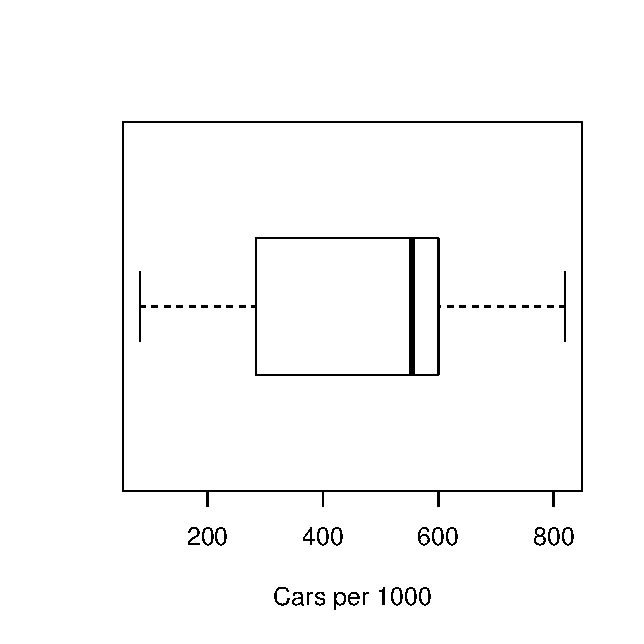
\includegraphics[width=6cm]{figure/f3_1-1.pdf}
   \caption{Boxplot of Cars per 1000}
   \label{fig:f3_1}
\end{figure}

{\bf{3. }} When we compare the median to the mean, we find the median (555) is greater the mean (472.6).  Therefore, we can say the the dataset is left skewed.

  \end{solution}

  \begin{exercise} % 8

You are a researcher for a mid-sized city. You collected six types of \\ variables from a random sample of students from a large university.  These variables include:

  \begin{enumerate}
  \item their region of birth of country
  \item the extent they support marijuana \\ legalization (7=strong, 4=neutral, \\ 1=weak)
  \item the weekly amount of money spent on cafeteria food
  \item number of movies they watched per \\ week
  \item quality of cafeteria food at their university (10=excellent, 0=bad)
  \item religious affiliation.
  \end{enumerate}

Select the  appropriate measures of central \\ tendency for each variable.


% \end{minipage}

% \vspace{1cm}
%     \framebox[5cm][l]{ Answer: }

  \end{exercise}
  \begin{solution}   % 8

  {\bf{(1. )}} Mode  {\bf{(2. )}} Median  {\bf{(3. )}} Mean  {\bf{(4. )}} Mean  {\bf{(5. )}} Median  {\bf{(6. )}} Mode

  \end{solution}

%' \pagebreak
  \begin{exercise} % 9

% Requires the booktabs if the memoir class is not being used
\begin{table}[htbp]
   \centering
   \caption{Find appropriate measures of central tendency}
   %\topcaption{Table captions are better up top} % requires the topcapt package
   {\tiny{
   \begin{tabular}{@{} cccccc  @{}} \hline % Column formatting, @{} suppresses leading/trailing space
   Student & Birth  & Expense & Movies & Food & Religion \\ \hline
   a & West  & 43 & 4 & 6 & Cath. \\
   b & MW  & 51 & 3 & 5 & Other \\
   c & South  & 65 & 14 & 0 & Other \\
   d & South  & 52 & 0 & 10 & Prot. \\
   e & North  & 48 & 1 & 6 & Jew \\
   f & North  & 62 & 5 & 8 & Prot. \\
   g & MW  & 47 & 7 & 1 & None \\
   h & South  & 45 & 10 & 2 & Cath. \\
   i & North  & 39 & 14 & 7 & Prot. \\
   j & North  & 33 & 0 & 10 & Prot. \\ \hline
   \end{tabular}
   }}
   \label{tab:t3_3a}
\end{table}

  Using the dataset from Table 3.3, determine the value of the central tendency measures for each variable.

   % \framebox[5cm][l]{ Answer: }
  \end{exercise}
   \begin{solution}  % 9

     {\bf{Birth}} Mode=``North'';   {\bf{Expense}} Mean=48.5; {\bf{Movies}} Mean=5.8; {\bf{Food}} Median=6;  {\bf{Religion}} Mode=``Protestant''

   \end{solution}

% \newpage
  \begin{exercise} % 10

As a leader of a Kalamazoo social services agency that employs 20 staff members, you are concerned that your staff has an increased case load of clients \\ compared to 10 years ago.  The case load of each worker is reported in the following table (Table 3.4) for years 2005 and 2015.

% Requires the booktabs if the memoir class is not being used
\begin{table}[htbp]
   \centering
   \caption{Case Loads Comparison}
   %\topcaption{Table captions are better up top} % requires the topcapt package
   {\tiny{
   \begin{tabular}{@{} ccccccccccc  @{}} \hline % Column formatting, @{} suppresses leading/trailing space
   2005 & 50&64&55&64&60&53&56&50&51&45 \\ & 46&46&50&56&63&65&53&54&58&69 \\ \hline
   2015 & 57&47&46&59&59&50&57&52&41&66 \\ & 65&52&57&75&65&76&43&56&52&67 \\ \hline
   \end{tabular}

   \label{tab:t3_4a}
   }}
\end{table}

  Has the average case load increased, \\ decreased, or stayed the same?

   \vspace{2mm}
     \framebox[5cm][l]{ Answer: }
  \end{exercise}
  \vspace{2mm}
  \begin{solution} %10


The mean for 2005 is 55.4.
The median for 2005 is 54.5.
The mean for 2015 is 57.1.
The median for 2015 is 57.

  \end{solution}

  \begin{exercise} % 11

  The admissions \\ department at WMU gave 25 randomly selected freshmen a national prejudice survey.  The racial prejudice index scores  will be used in three years to see if higher education affects prejudice.

% Requires the booktabs if the memoir class is not being used
\begin{table}[htbp]
   \centering
   %\topcaption{Table captions are better up top} % requires the topcapt package
   {\small{
   \caption{Freshmen Racial Prejudice Index}
   \begin{tabular}{@{} ccccc  @{}} \hline % Column formatting, @{} suppresses leading/trailing space
   45 & 30 & 35 & 30 & 42 \\
   50 & 43 & 40 & 32 & 48 \\
   9  & 13 & 10 & 11 & 11 \\
   40 & 26 & 39 & 38 & 44 \\
   32 & 37 & 41 & 27 & 22 \\ \hline
   \end{tabular}

   \label{tab:t3_12}
   }}
\end{table}

  Calculate the mean and median scores of \\ these data from Table 3.5.

	\vspace{2mm}
    \framebox[5cm][l]{ Answer: }
	\end{exercise}
	\begin{solution}   % 11

	The mean is
[1] 31.8


	The median is
[1] 35


	\end{solution}

	  \begin{exercise} % 12

The same 25 students \\ completed the same survey during their senior  year.  Compute the mean and median for this second set of scores, and compare them to the scores from four years earlier.   What happened?

% Requires the booktabs if the memoir class is not being used
\begin{table}[htbp]
   \centering
   %\topcaption{Table captions are better up top} % requires the topcapt package
   {\small{
   \caption{Senior Racial Prejudice Index}
   \begin{tabular}{@{} ccccc  @{}} \hline % Column formatting, @{} suppresses leading/trailing space
   50 & 27 & 31 & 35 & 41 \\
   11 & 45 & 50 & 37 & 43 \\
   11 & 9  & 10 & 20 & 10 \\
   35 & 10 & 30 & 41 & 40 \\
   15 & 30 & 40 & 26 & 21 \\ \hline
   \end{tabular}
   }}

   \label{tab:t3_6a}
\end{table}

  Calculate the mean and median scores of \\ these data.

	\vspace{2mm}
    \framebox[5cm][l]{ Answer: }
	\end{exercise}
	\vspace{2mm}
	\begin{solution}   % 12



  The mean is 28.72, and the median is 30

	\end{solution}

	\begin{exercise} % 13

A local social service \\ agency has started a sex education course for teen girls.  The girls took a 20-question exam for general information about sex, anatomy and physiology upon entry and again after completing the course.  Table 3.7 has the listing of scores of a random sample of 15 \\ girls.

Calculate the mean and median of the pre and post test scores and comment on the results.

 % latex table generated in R 3.2.1 by xtable 1.7-4 package
 % Wed Sep  2 09:06:12 2015
\begin{table}[ht]
 \centering
 \caption{Pre and Post Test Results}

 {\small{
 \begin{tabular}{@{} rrrrr @{}}
   \hline
   case & posttest & pretest & difference \\
   \hline
    1 &  12 &   8 &   4 \\
      2 &  13 &   7 &   6 \\
      3 &  12 &  10 &   2 \\
      4 &  19 &  15 &   4 \\
      5 &   8 &  10 &  -2 \\
      6 &  17 &  10 &   7 \\
      7 &  12 &   3 &   9 \\
      8 &  11 &  10 &   1 \\
      9 &   7 &   5 &   2 \\
     10 &  12 &  15 &  -3 \\
     11 &  21 &  13 &   8 \\
     12 &   5 &   4 &   1 \\
     13 &  15 &  10 &   5 \\
     14 &  11 &   8 &   3 \\
     15 &  20 &  12 &   8 \\
    \hline
 \end{tabular}
 }}

 \label{tab:t3_14}
\end{table}

	\vspace{2mm}
    \framebox[5cm][l]{ Answer: }
	\end{exercise}
	\vspace{2mm}
	\begin{solution}  % 13




	The pretest mean is  9.3333333


	The pretest median is 10


	The posttest mean is	12.9333333


The pretest median is 12

	\end{solution}

	\begin{exercise}   % 14

	The acidity or alkalinity of a solution is measured using pH.  A pH less than 7 is acidic; a pH greater than 7 is alkaline.  The following data represent the pH in samples of bottled water and tap water.

\begin{table}[ht]
 \centering

	{\small{             % \footnotesize{
	\caption{Source: Emily. McCarney, \\ Joliet College}
 \begin{tabular}{@{} rrcrr @{}}
     % \multicolumn{4}{c}{TAP    |    BOTTLED}  \hline
  % \multicolumn{2}{Tap} & | & \multicolumn{2}{Bottled} \hline
   Tap &  & | & Bottled  & \\ \hline
   7.64 & 7.45 & | & 5.15 & 5.28 \\
   7.45 & 7.10 & | & 5.09 & 5.26 \\
   7.47 & 7.56 & | & 5.26 & 5.13 \\
   7.50 & 7.47 & | & 5.20 & 5.26 \\
   7.68 & 7.52 & | & 5.02 & 5.21 \\
   7.69 & 7.47 & | & 5.23 & 5.24 \\
    \hline
 \end{tabular}
 }}
   \label{tab:t3_15}
 \end{table}

\begin{enumerate}
 \item Calculate the mean  of the tap water.
 \item Determine the median of the tap water.
 \item Comment on the results.
\end{enumerate}
  \end{exercise}
%   \begin{solution}  % 14
%
%
%   \end{solution}

\begin{exercise}  % 15

\begin{table}[ht]
 \centering
            % \footnotesize{
	\caption{Source: Google}
 \begin{tabular}{@{} lc @{}}
     % \multicolumn{4}{c}{TAP    |    BOTTLED}  \hline
  % \multicolumn{2}{Tap} & | & \multicolumn{2}{Bottled} \hline
  Ethnic 	& Mean household \\ 
  category & income (K \$) \\ \hline
  Asian (AA) & 114 \\
  Black (BA) & 59 \\
  Hispanic or Latino (HA) & 68 \\
  White (WA) & 90 \\
    \hline
 \end{tabular}
   \label{tab:t3_16}
 \end{table}

\begin{enumerate}
\item Based on this table, give two reasons why this income disparity.
\item Does the mean salary of BA say that BA earn less than WA? Why or why not?
\item Is it possible for BA and WA to earn the same salary, but have different mean \\ salaries?
\end{enumerate}

\end{exercise}
\begin{solution}  % 15

\begin{enumerate}
\item   1) less education, 2) less wealth, 3) poorer health, 4) racism 
\item Does median age of BA say that BA die younger than WA? Why or why not?  
\item Is it possible for BA and WA to die the same age, but have different median \\ ages?
\end{enumerate}
\end{solution}



\end{exercises}

\onecolumn


%!Rnw root = ../../Main.Rnw

\chapter{Threats to Valid Comparisons}
\label{chap:ch4}

\section{Objectives}

After completing this part, students should be able to:

\fbox{\parbox{14cm}{

 \begin{enumerate}
 \item Know the difference between association and causation. 
 \item Understand how confounders can affect the results of a study.
 	\end{enumerate}
 }}

\section{Hidden Confounder}  \index{confounds}

In 1992, a research study ``Lower extremity fractures in motor vehicle collisions:
Influence of direction of impact and seatbelt use'' by Dischinger, P., Cushing, B. and Kerns, T. was published in the 36th Proceedings of the Association for the Advancement of Automotive Medicine.  It involved data analysis of the trauma-center population in Maryland.  Some of the conclusions were:

\begin{enumerate}
   \item there was a higher incidence of lower extremity injury in frontal collisions,
   \item seatbelt use was not effective in preventing lower extremity fractures, and
   \item there was a higher incidence of lower extremity fracture among women.
\end{enumerate}

The conclusion (3) is interesting.  It begs the follow-up question: ``Why do women have higher rates of leg fractures?''  Is it because they drive faster, or apply brakes more slowly, or have weaker bones?  It turns out that these are false questions -- they presume that gender is the variable that causes higher leg fractures.  

Researchers proposed an explanation in a follow-up study with the same lead author: `Lower extremity fractures in motor vehicle collisions: The role of driver gender and height' by Dischinger, P.C., Kerns, T.J., Kufera, J.A. Accident Analysis \& Prevention Volume 27, Issue 4, August 1995.

\begin{quotation}
Abstract: In a previous study it was noted that there was a higher incidence of lower-extremity fractures among women drivers. Analyses were based on a linkage between trauma registry and police crash report data. The present study addresses the issue of whether the differences noted are attributed to driver gender or are merely a reflection of differences in driver's height. An inverse association was noted between driver height and the incidence of lower-extremity fractures. Those shorter than average (5'7'') for this population had a 64\% increase in a lower-extremity fracture, which can be mainly attributed to ankle/tarsal injuries. Thus, the incidence of these injuries appears to be a function of driver height, with an increase among shorter drivers, most of whom are women.
\end{quotation}  \citep{dischinger1995}

It turns out that height was the culprit, but it initially looked like gender because height and gender have a strong link.  The following \textit{pathway graph} describes the true relationship:

\begin{eqnarray*}
\texttt{Height} & \Rightarrow & \texttt{Leg Fracture} \\
\updownarrow &  & \\
\texttt{Gender} & &
\end{eqnarray*}

But the association between height and gender led us to believe the wrong relationship:

$$ \texttt{Gender} \Rightarrow  \texttt{Leg Fracture} $$

The symbol $\Rightarrow$ represents ``cause-and-effect'' while $\updownarrow$      represents ``association.''

In this situation, leg fracture rate is the outcome, variable gender is the probable cause.  The hidden variable height is called a \textbf{confounder}, or a confounding variable.

\fbox{\parbox{14cm}{
\textbf{Confounding Variable:} \\
A confounder or confounding variable is a third variable that is associated with both the probable cause and the outcome.  It can lead us to a wrong conclusion about the cause-and-effect relationship.
}}

\subsection{Apples and Oranges}

Now, why do unknown confounders belong in a chapter on threats to valid comparisons?  They are one of the most significant sources of (often unknowingly) invalid comparisons.  It seemed fair to compare leg fracture rates of men and women, didn't it?  What's wrong with that?  Unfortunately, concerning leg fracture rates, it was a case of comparing apples to oranges -- women as a group is shorter than men!  Of course, in the 1992 study, the investigators did not know that height would make a difference.  Women also tend to weigh less, smoke less, drink less, have longer hair, and wear higher heels.  Which of these would make a difference, i.e., be potential confounders?

Confounders are a big problem in comparison studies.  Some confounders may remain hidden, but it is critical that the researchers identify and control for potential confounders as much as possible.  Does smoking cause lung cancer?  When comparing smokers to nonsmokers, it is easy to show that smokers have higher lung cancer rates.  But as a group, they exercise less than nonsmokers.  They drink more coffee than nonsmokers.  Can the exercise or the coffee or the combination be the culprit?  Furthermore, smokers tend to be male, older, and drive in the winter with their car windows open.  There are plenty of confounding variables even in this comparison.

\subsection{In the news}

The STATS website (http://www.stats.org/) is dedicated to correcting ``scientific
misinformation in the media and public policy resulting from bad science,
politics, or a simple lack of information or knowledge.''  The following is an excerpt from an article written by Rebecca Goldin and Jing Peng in August 2010.  What is the confounding variable?  The probable cause? The outcome variable?

\begin{quotation}
\textbf{If you take Viagra, will you get an STD?} \\
Rebecca Goldin Ph.D. and Jing Peng, August 2, 2010 

Judging from recent headlines, it seems clear:  ``Sex Diseases Tripled in Men 40 or Older Taking Viagra, Cialis, Study Says'' reports Bloomberg; ``Older Viagra Users More Likely to Get STDs'' says the Chicago Sun-Times, presumably comparing older Viagra users with older non-Viagra users.  And Health Day was even more explicit, saying ``Drugs Like Viagra Linked to Higher Rates of STDs.''  The next logic behind the claim seems persuasively apparent: if men who take Viagra are having more sex, then they have inevitably increased their risk of catching a sexually transmitted disease (STD). But is this the case?

The study compared men who took erectile dysfunction (ED) drugs with those who did not.  Researchers found that ED drugs such as Viagra are linked to higher rates of STDs among older men, but not older women, especially after the introduction of Viagra in 1998.  A study published in the July 6 issue of the Annals of Internal Medicine was the first to examine the relationship between ED drugs and STDs. But its findings turn out to be far different than media accounts would have you believe.

The main problem in the coverage is the direct suggestion that taking Viagra is associated with STDs, as opposed to being the sort of person who takes Viagra.

There is a critical distinction. To see what it means, let's go backward in time and compare STD rates among people who plan to take Viagra but haven't and people who are not planning on taking Viagra. This quick comparison is what the authors of the research article did; they combed medical records for people who filled prescriptions for ED drugs and compared STD rates for these people before filling their prescription to the STD rates of people who did not subsequently fill a prescription for Viagra.  It turns out that the rate of STDs is higher among people who intend to take it.  In other words, the drug is absent, but those people who will take Viagra within a year are already at higher risk of STDs.

In fact, compared to those who don't take ED drugs, those who plan to take Viagra had a slightly higher rate for STDs, an odds ratio (OR) of 2.80; 95\% confidence interval CI, 2.10 to 3.75, than those who actually take it (OR) 2.65, CI, 1.84 to 3.81, though the difference was not significant. It means that the drug had no discernable effect on STD rates for this group of men.
\citep{goldin2010}
\end{quotation}


The paper goes on with detailed analysis, but the main point has been stated.  To summarize the conclusions of the study:

\begin{enumerate}
	\item Taking ED drugs do not increase the rate of STD's
	\item The type of people who take ED drugs are different from people who do not.

	\begin{eqnarray*}
\texttt{Person type} & \Rightarrow & \texttt{STD} \\
\updownarrow &  & \\
\texttt{ED drugs} & &
\end{eqnarray*}

instead of the (admittedly more sensational) relationship implied by the headlines.

\end{enumerate}

% \pagebreak

\section{Key Words}

\fbox{\parbox{14cm}{

\begin{minipage}[ht]{6cm}

\begin{itemize}
\item association
\item cause
\end{itemize}
\end{minipage} \hfill
\begin{minipage}[ht]{6cm}

\begin{itemize}
\item confounders
\item effect
\end{itemize}

\end{minipage}

}}

% \newpage
\twocolumn
\section{}

\begin{exercises}
  \begin{exercise} % 1

A study says, ``Slightly \\ overweight people live longer than thin people.''

\begin{enumerate}
  \item The headline implies cause-and-effect, \\ not just association, i.e. ``if you are thin, you should try to gain weight.''  When comparing lifespan of slightly over- \\ weight and thin people, can you think of possible confounders?
  \item Using one confounder from your \\ answer(s) in (1), draw a pathway graph depicting the possible relationship between confounder, possible cause, and \\ outcome.
\end{enumerate}

	\end{exercise}
	\begin{solution}  % 1

	  $H_0: \mu = 6.2$ vs. $H_A: \mu \neq 6.2$
	\end{solution}

  \begin{exercise} % 2

A study that appeared \\ in the American Journal of Cardiology \\ (March 15, 2003) found out that generally, ``heart attack survivors who owned a dog had better heart function post-heart attack than those who did not own a dog.''

\begin{enumerate}
  \item Does a dog help a heart heal faster?  \\ Can you think of possible confounders?
  \item Using one confounder from your \\ answer(s) in (1), draw a pathway graph depicting the possible relationship between confounder, possible cause, and \\ outcome.
\end{enumerate}

	\end{exercise}
	% \begin{solution}  % 2
	%
	%     $SE = \frac{0.7}{\sqrt{25}} = 0.14$  \\
	%     $t = \frac{(5.9 - 6.2)}{0.14} = -2.14$
	%
	% \end{solution}

  \begin{exercise} % 3

A study says, ``People \\ who  consider themselves depressed eat more \\ chocolate than people who consider them- \\ selves otherwise.''

\begin{enumerate}
\item The headline implies cause-and-effect, \\ not just association, i.e., ``if you are depressed, you will tend to eat more \\ chocolate.''   When comparing chocolate consumption of depressed versus not-depressed, can you think of possible  \\ confounders?
  \item Using one confounder from your \\ answer(s) in (1), draw a pathway graph depicting the possible relationship between confounder, possible cause, and \\ outcome.
\end{enumerate}
  \end{exercise}
  \begin{solution}  % 3


    From the distribution of $t$, using row df = 24 and column 0.025, CV(t) = 2.064.
  \end{solution}


  \begin{exercise} % 4

The next four questions \\ refer to the following scenario.  In a recent \\ statewide election, 55 percent of the voters rejected a proposal to institute a state lottery.  In a random sample of 150 urban precincts, 60 percent of the electorate rejected the \\ proposal.  Can you think of possible  \\ confounders? 
  \end{exercise}


\end{exercises}
\onecolumn


%!Rnw root = ../../Main.Rnw

\chapter{Study Designs}
\label{chap:ch5}

\section{Objective}

After completing this part, students should be able to:

\fbox{\parbox{14cm}{

 \begin{enumerate}
 \item Grasp the basics of good experimental design
 \item Understand the importance of randomized trials (RT).
 \item Comprehend the meaning of double blind, randomized controlled \\ trials (RCT).
 \item Recognize the difference between observational studies and randomized \\ controlled trials.
 \item Perceive the need for case-controlled studies.
 \item Grasp the need for case-crossover studies. 
 	\end{enumerate}
 }}

\section{Randomized trials}

In the previous chapter, we covered unknown confounders, one of the most critical threats to valid comparisons in statistics. In this chapter, we will explore elements of study design that help statisticians deal with the danger of bias posed by hidden confounders. One of the most important aspects of many study designs is appropriate randomization in the selection of subjects for the study, and to different groups within the study. Without such randomization, results of data analyses can be biased. Let's see by way of example how randomization can help us address the threat of results biased by hidden confounders.

Recall the diet study discussed previously: ``Comparison of the Atkins, Zone, Ornish, and LEARN Diets for Change in Weight and Related Risk Factors Among Overweight \\ Premenopausal Women The A TO Z Weight Loss Study: A Randomized Trial'' by C.D. Gardner, et al. (JAMA, Vol. 297, pp. 969-77, March 2007)

\begin{quotation}
 \textbf{Objective:} \\ To compare four weight-loss diets representing a spectrum of low to high carbohydrate intake for effects on weight loss and related metabolic variables. Design, Setting, and Participants Twelve-month randomized trial conducted in the United States from February 2003 to October 2005 among 311 free-living, overweight/obese (body mass index, 27-40) nondiabetic, premenopausal women.  Intervention participants were randomly assigned to follow the Atkins (n=77), \\ Zone ($n = 79$), LEARN ($n = 79$), or Ornish ($n = 76$) diets and received weekly instruction for 2 months, then an additional 10-month follow-up.
\end{quotation}

Here is an example of a randomized trial or randomized experiment.   Subjects entering the test are randomized, using a virtual roll of a die, into one of several treatment groups.

The randomization into groups eliminates the main threat to valid comparisons: \\ confounders.  How?  By making the comparison groups similar to each other in all aspects, except for the treatment.  Think about it.  If you ask for volunteers to each treatment group, then most of the meat-eaters would go to the Atkins group, and most of the vegetarians would go to the Ornish group.   Would it then surprise you if one group had, say, more Asians than another group?  Or more smokers?  Or less physical activity?  Randomized assignments, instead of volunteering, is the best way to get balanced groups in the factors that we think might matter and achieves balance in all other factors we have not even considered.

Table \ref{tbl51} on page \pageref{tbl51} presents the characteristics (averages or frequencies) of the subjects after randomization, but before treatment has started.  Observe how randomization has achieved a right balance between groups in demographic and anthropometric variables (using either percentages or averages and standard deviations, respectively), and known health risk factors.  All other variables, essential or not, like IQ, shoe size, and preference for country music would also tend to be balanced, thus providing a level of protection against unknown confounders.

\fbox{\parbox{14cm}{
To safeguard against potential \textbf{confounders}, comparison groups should be \textbf{similar} in all factors except for treatment itself.  \textbf{Randomization} is the best way to achieve the goal.
}}

\begin{table}[ht] 
\caption{Baseline Participant Characteristics}
\begin{tabular}{@{} lrrrr @{}} \hline
         & Atkins & Zone & LEARN & Ornish \\ \hline
Number of Subjects       & 77     & 79   &    79 &  76 \\
\textbf{Demographics}, No.(\%)  &  &  &  &  \\
Race/ethnicity &  &  &  &  \\
\hspace{3mm} Asian/Pacific Islander & 7(9) & 9(11) & 6(8) & 8(10) \\
\hspace{3mm} Black                  & 2(3) & 7(9)  & 6(7) & 4(5) \\
\hspace{3mm} Hispanic               & 7(9) & 8(10) & 7(9) & 11(14) \\
\hspace{3mm} White                  & 59(76) & 52(66) & 59(75) & 52(69) \\
\hspace{3mm} Other                  & 2(3)   & 3(4)   & 1(1)   & 1(1) \\
Smokers      & 2(3)   & 4(5)   & 4(5)   & 3(4) \\
Age, yrs; $\bar{x} (SD)$ & 42(5) & 40(6) & 40(7) & 42(6) \\
Education, yrs; $\bar{x} (SD)$ & 16(2) & 16(2) & 16(2) & 16(2) \\
Physical activity {\scriptsize{(kcal/kg per day)}}; $\bar{x} (SD)$     & 34(6)  & 34(6)  & 34(5)  & 35(7) \\
\textbf{Anthropometrics} $\bar{x} (SD)$   &  &  &  & \\
Weight, kg             & 86(13) & 84(12) & 85(14) & 86(10) \\
Body fat, \%           & 41(6)  & 40(6)  & 38(6)  & 40(6) \\
Body mass index        & 32(4)  & 31(3)  & 31(4)  & 32(3) \\
Waist-hip ratio        & .843(.067) & .841(.068) & .839(.066) & .840(.060) \\
\textbf{Cardio. disease risk factors} & & & & \\
LDL-C, mg/dL           & 109(29) & 114(32) & 104(29) & 111(27) \\
HDL-C, mg/dL           & 53(14)  & 52(11)  & 51(11) & 50(11) \\
Triglycerides, mg/dL   & 125(78) & 123(98) & 119(73) & 118(62) \\
Non-HDL-C, mg/dL       & 134(33) & 139(39) & 127(34) & 135(33) \\
Ratio of total cholestrol to HDL-C & 3.7(1.0) & 3.8(1.1) & 3.6(1.0) & 3.8(1.0) \\
Fasting insulin, U/mL & 10(7) & 10(7) & 10(8) & 10(5) \\
Fasting glucose, mg/dL & 92(9) & 94(20) & 96(17) & 93(13) \\
\textbf{Blood pressure, mmHg}; $\bar{x} (SD)$ & & & & \\
Systolic & 118(11) & 115(13) & 116(12) & 116(10) \\
Diastolic & 75(8) & 74(9) & 75(9) & 75(8) \\
Metabolic syndrome, No. (\%) & 22(29) & 20(25) & 29(37) & 27(36) \\ \hline
\end{tabular}
  \label{tbl51}
\end{table}

\subsection{Double blind randomized controlled trials (RCT)}

Scientific studies should be randomized as described above whenever possible. But it might surprise you to learn that randomization is just one way to address hidden confounders and bias in clinical trials. The present section will cover \textit{controls and blinding}, two critical elements in study design that address confounders and bias.

Thus far, we’ve discussed how vital randomly assigning subjects in a study to groups within that study is to overcoming bias, but study designers should be aware that there is some luck involved in randomization. It is not always likely, but it is possible, that even the best randomization techniques leave unknown confounders present across all \textit{subjects} within the study. We may be selecting subjects for the study from a population where they all have a confounding characteristic in common. In such a case, it would not help us much to randomly assign subjects to different groups of the study since all the groups would end up exhibiting the same bias regardless as to how we assigned the subjects. Imagine attempting to conclude whether a medication is effective in treating the common cold by studying only subjects who have some particular resistance to the cold. No patients would get severe colds, or if they did, they would not manifest many cold symptoms like coughing, sneezing, or a runny nose. Sounds hard to study such subjects, right? Yes, the immune response confounder makes these subjects hard to explore, but this problem is solvable. Scientists need more \textit{control} in assessing such matters and their hidden confounders, so control \textit{groups} are added to scientific studies to correct for this problem.

Control groups are groups of subjects within the study that are not expected to respond in the same way as the treated groups.  For instance, control groups in medical studies are often groups of patients given inert placebos or ``sugar pills'' instead of active medications. Since the study directors do not provide these groups with the active medication, such groups are not expected to exhibit effects as strong as the treatment groups who receive medications.  We would not expect patients who receive sugar pills to miraculously feel relief from their cold symptoms in the same way patients who receive a new alternative to pseudoephedrine might. Even when such placebo groups do exhibit effects like the expected treatment effects, which can be due to the placebo effect or other hidden confounders (different resistance to the cold), the presence of these control groups within the study gives researchers a valid point of comparison. It is true that both the placebo and medicated groups selected from our cold-resistant population of patients would be asymptomatic. However, even though there is less sneezing when comparing the medicated and unmedicated groups, the response allows scientists to determine if it is just the patients' robust immune responses or the psychological impact of taking a pill is responsible, or if the medication is exceptionally effective at treating the cold.


\begin{figure}[ht]
   \centering
   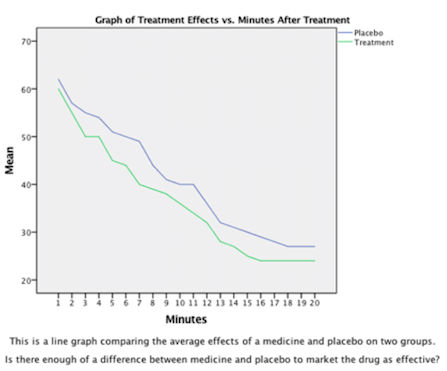
\includegraphics[width=10cm]{chapters/Chapter_5/ext_figure/timeVsRx.png} % requires the graphicx package
   % \caption{example caption}
   % \label{fig:example}
\end{figure}

When one of the comparison groups in a study is a control group or placebo, randomized trials are sometimes called randomized controlled trials, or randomized controlled experiments. As much as possible, researchers try to conduct \textit{double-blind} randomized controlled trials, when neither the doctor nor the patient knows what treatment the patient is receiving.  In the common cold example, some patients get a sugar pill or placebo while others get a new alternative medication thought to treat cold symptoms.  (The critical point to remember here is that in a double-blind-controlled experiment both the \textit{patients} and \textit{doctors} have no idea if a patient is receiving the sugar pill/placebo or the cold medicine.) This method gives each patient a pill that looks identical regardless as to whether it is the inert placebo or the active drug.

% \begin{minipage}[ht]{5cm}

\begin{figure}[ht]
   \centering
   
\includegraphics[width=2cm]{chapters/Chapter_5/ext_figure/placebo.png}
   
\includegraphics[width=2cm]{chapters/Chapter_5/ext_figure/medicine.png}
   % requires the graphicx package
    \caption{\textbf{Placebo} or \textbf{Medicine}}
   % \label{fig:example}
\end{figure}
% \end{minipage}

Can you spot the difference? -- Single Blinding.  Can your doctor? -- Double Blinding. 

This double-blinding is essential because it offers additional protection against bias. In such studies, all groups have the same frame of mind (as opposed to knowing you are not getting the new drug). Similarly, the experimenter has the same frame of mind evaluating patients from each group. You might wonder, isn't it enough to single-blind the study, to make sure that just the patients are unaware whether they received the placebo or medicinal pill? No, it is not. Imagine an experimenter who administers both the placebos and medications but does so know which is which. That researcher might unintentionally treat these two groups differently, perhaps just by spending an extra minute with patients from the medicated treatment group or by approaching them with a little more enthusiasm. It's this sort of unwitting behavior that can invite bias into the study.

\section{Observational studies}

In many cases, the treatments being compared cannot be assigned, and hence cannot be randomized.  The study involving women and leg fractures is an example.  We compared leg fracture rates of two groups, men, and women.  Whenever a new subject enters the study, e.g., by having a car accident, we \textit{observe} what gender they belong to, instead of randomly assigning it to control or treated group.  Studies like these are called \textit{observational studies}, as opposed to randomized experiments.  In the hierarchy of scientific evidence, observational studies are not as reliable as randomized trials are regarded as the gold standard. Since the subjects of observational studies assign themselves to a different group, there may be a selection bias that leads to confounders (like the women in the leg-fracture-study being shorter).  We can control the effects of known confounders in the analysis.  For example, we can compare leg fracture rates of men and women with the same heights.  Investigators will need to anticipate potential confounders and control for them. We enumerate common reasons for nonrandomized studies:

\begin{enumerate}
\item Assigning treatment is impossible (e.g., to compare fracture rates between men and women, we cannot randomize subjects into the comparison groups).

\item Assigning treatment is unethical (e.g., to compare cancer rates of smokers and nonsmokers, we do not want to randomize subjects into smoker-nonsmoker     comparison groups.)  In other words, we do not want to force nonsmokers to smoke.

\item Assigning treatment is impractical (e.g., the outcome is a rare event like cancer or stroke, and a randomized trial would need too many subjects and too much time).  In cases like these, a case-control study is generally the way to go.
\end{enumerate}

\fbox{\parbox{14cm}{
\textbf{Observational studies} are conducted when \textbf{randomization} to treatment groups  \\ is \textbf{impossible}, \textbf{unethical}, or \textbf{impractical}.
}}

Returning to the leg-fracture example, we stick to observational studies in such a case for two reasons. As described above, it's impossible to perform the research any other way with the data collected. But we also \textit{should not} elect to collect the data in a randomized manner.  In other words, we should not even try to get the bias-reducing benefits of randomization because of ethical constraints. To perform randomized clinical trials in this study of leg fractures, we would need to randomly select subjects whose legs \textit{would} be broken for the sake of the study. Causing suffering like this is prohibited by several codes of ethics like the Nuremberg Code, a system of research ethics drafted after the Nuremberg trials of Nazi war criminals.  These criminals included scientists who designed and performed inhumane experiments. Beyond the official ban, though, such research is wrong in its causing undue suffering and its infringement upon fundamental human rights.

Another reason we may conduct an observational study is that they can be more practical compared to randomized controlled trials. It can be due to the constraints of a rare disease, or the cost of a randomized study would entail.  A researcher might want to study whether regular exercise can prevent a rare form of cancer.  Randomization and control here would require that we randomly select patients first, group them along exercise programs (say regular, irregular, and no exercise), and wait to see how the different groups respond (do the exercise groups have significantly fewer cases of cancer?).  This study might not work out at all because, since the cancer is rare, it's possible that no or very few of our subjects will get cancer.  It also may take many years before cancer would appear.

This study would be quite time-consuming and labor-intensive. Imagine all the financial resources that would be required to do all that exercise-monitoring over all the patients and years! This experiment brings us to our second point that observational studies are practical because they tend to be less costly than randomized controlled trials. Companies often use statistics to generate revenue, but they tend to do this not by randomized experiments, but by analyses of marketing data they collect through sales or surveys. Nonrandom observational studies like analyses of sales data are a relaxed approach in that all they require are a data collection apparatus and a statistician. For instance, clothing designers want to keep up with trends in consumer spending but might sell hundreds of different garments to thousands of outlets across the world. When sales of one item begin to slip, it might be difficult to notice amidst all the chaos of such a business enterprise. A statistician can help here by analyzing the proportions of revenue generated by each garment from month to month and making recommendations about which products to push when. The statistician might even find a style or color-based patterns that repeat themselves seasonally, allowing the company to adjust before their sales ever begin slipping.

\subsection{Case-control studies}

Instead of randomizing subjects into diet groups and then comparing the weight loss outcome, a case-control study would look for people in the population who lost weight, and then ask them what diet they used.  Thus, you start with the \textit{outcome} and then work back to the type of treatment.  These are also classified as \textit{retrospective} studies because they look back and compare weight loss or disease rates of various procedures.  Randomized experiments are necessarily \textit{prospective}, in the sense that you randomize treatment and then later see which groups lost more weight or had more disease.

We frequently use case-control studies because they are cheaper and easier to conduct since it generally requires a survey of a database, instead of expensive and time-consuming recruitment and handling of subjects.  There are plenty of successful case-control success stories in the scientific literature.

The first study formally linking lung cancer to smoking was a 1950 case-control study ``Smoking and Carcinoma of the Lung'' by Richard Doll and A. Bradford Hill(British Medical Journal, 1950 September 30; 2(4682): page 739--748).  Using patients in 20 hospitals in London, they found that lung-cancer patients had higher rates of smokers than a comparable control group of patients.   For example, among district hospitals, 48 out of 98 lung cancer patients smoked 15 or more cigarettes daily.  In contrast, only 30 out of 98 non-cancer patients smoked 15 or more cigarettes daily.  

In general, case-control studies can conclude a link or `association' but are not able to prove `causation.'   However, case-control studies provide initial evidence that can generate resources for more rigorous studies like double-blind, randomized controlled trials.  In the case of smoking and lung cancer, randomized trials are unethical, but given the eventual results of multiple studies, the scientific community now accepts that smoking causes lung cancer.  
\citep{doll1950}

\subsection{Case-crossover studies}

Sometimes, a subject can be its control.  This method is called a case-crossover study because of subjects in the treatment group ``crossover'' to the control group.  An example is a 1997 study linking cell phone use to car accidents: ``Association between cellular-telephone calls and motor vehicle collisions'' by D.A. Redelmeier and R.J. Tibshirani (The New England Journal of Medicine, 1997 Feb 13; Vol 336, pp. 453-8).  The subjects were people who reported a collision to the North York Collision Reporting Centre between July 1, 1994, and August 31, 1995, Among these, 742 had cell phones and consented to participate in the study.  Instead of asking each person whether they were using their cell phone during the time of the collision (an unreliable method), the investigators examined their detailed phone billing records.  The results of the experiment follow below:

\begin{quotation}
Overall, 170 subjects (24 percent) had used a cellular telephone during the 10-minute period immediately before the collision, 37 (5 percent) had used the telephone during the same period on the day before the collision, and 13 (2 percent) had used the telephone during both periods. The crude analysis indicated that cellular-telephone activity was associated with a relative risk of a motor vehicle collision of 6.5 (95 percent confidence interval, 4.5 to 9.9).  The primary analysis, adjusted for intermittent driving, indicated that cellular-telephone activity was associated with a quadrupling of the risk of a motor vehicle collision (relative risk, 4.3; 95 percent confidence interval, 3.0 to 6.5).
\end{quotation}  \citep{redelmeier1997}

\section{Key Words}

\fbox{\parbox{14cm}{
\begin{minipage}[ht]{66mm}
\begin{itemize}
\item randomized trial
\item double blind randomized trial
\item observational studies
\end{itemize}
\end{minipage} \hfill
\begin{minipage}[ht]{66mm}
\begin{itemize}
\item case-control studies
\item case-crossover studies
\end{itemize}
\end{minipage}
}}

% \newpage
\twocolumn
\section{}

\begin{exercises}
  \begin{exercise} %1

Give some examples of \\ studies where:

\begin{enumerate}
\item a randomized trial is impossible
\item a randomized trial is impractical \\ because of length of time the study      \\ would require
\item a randomized trial is impractical \\ because of the number of subjects \\ the study would require
\end{enumerate}


	\end{exercise}
	% \begin{solution}  % 1
	% 
	%   $H_0: \mu_1 = \mu_2$ vs. $H_0: \mu_1 \neq \mu_2$
	% \end{solution}

  \begin{exercise} % 2

Suppose a doctor is interested in investigating the causes of a \\ sporadic disorder that occurs in only \\ 0.00001\% (that is 1 in 10 million) of men.  What type of study would be necessary to establish the origins of the disease?  Is this type of research an appropriate choice for such a disease firmly?  Why or why not?

	\end{exercise}
	\begin{solution}  % 2

Randomized controlled experiments are necessary to establish the cause of such a disease firmly. For instance, we might see if potassium deficiency causes the disease, we may give our treatment group a potassium supplement every day. However, if the illness is rare, then it is impractical for us to use a randomized controlled experiment.  It would also be unethical to be influencing or causing disease in people potentially.  Additionally, we would have no guarantee that any subjects would even develop the disease if it is sporadic. Thus, observational studies may be the most appropriate choice unless scientific advances in, say, genetics are far enough along to make a more practical kind of randomized controlled experiment.

	\end{solution}

  \begin{exercise} % 3

What is a double-blind \\ study?  Give an example where double- \\ blinding is not possible.

    \end{exercise}
%     \begin{solution}  % 3
%
% % The test statistics is $|-1.66|$ and significance level is 1.8125.  Since the test statistic is less than the significance level, fail to reject $H_0$.
%     \end{solution}

  \begin{exercise} % 4

Some recent research \\ has  shown that patients who know they have \\ taken nothing more than an inert sugar pill still experience the placebo effect. Briefly describe a study design that might replicate \\ these results. What type of study would you choose? Should we consider different \\ groups?
  \end{exercise}
  \begin{solution}  % 4

A randomized controlled experiment is the ``gold standard of scientific knowledge'' so that it would be the best way to study this situation. We would study four groups of patients: group one would get a standard treatment for an illness, group two would get a placebo without being told it's a placebo, group 3 would get a placebo and told it's a placebo, and group 4 would get no treatment at all. This method would, interestingly, give controls both from the standard and no-treatment groups. The groups for primary comparisons would be the two groups that get the placebos and are either informed or not.

  \end{solution}

  \begin{exercise} % 5

What is the advantage of \\ case-control studies over randomized \\ controlled trials?

  \end{exercise}
%   \begin{solution}  % 5
% <label=lbl8-5, results='asis', echo=FALSE>>=
%   cv1 <- sprintf('%.2f', (qnorm(p=0.975)))
% @
%
%     Standard Normal (z) distribution, $Z = \pm cv1$.
%   \end{solution}

  \begin{exercise} % 6

A football organization is \\ concerned about the number of injuries to its athletes during games. The organization designs an observational study to help decide on rule changes that will reduce the risk of injury to players. They collect data and observe that a very high proportion of injuries incurred during the first moments of the \\ game during kickoff. The organization thus entertains the idea of changing the rules governing kickoff. Are there any hidden confounders that the organization should \\ address before making changes to  kickoff \\ rules? What are they, and how might they be treated?

	\end{exercise}
	\begin{solution}  % 6

Yes, there are potential confounders. For instance, it might be that players feel better rested at the start of a game, so they play harder and get injured more frequently because of this possibility. The organization could investigate the frequency of injuries that occur during later kickoffs in the game or to conduct small-scale randomized controlled experiments that change kickoff rules before recommending substantial sweeping changes.

	\end{solution}

	  \begin{exercise} % 7

What is the advantage of \\ randomized controlled trials over \\ case-control studies?

  \end{exercise}
  % \begin{solution}  % 7
  %
  %    $H_0: P_1 = P_2$ vs. $H_A: P_1 > P_2$
  % \end{solution}

	  \begin{exercise} % 8

Suppose the Kalamazoo \\ School District is proposing a 1 mil property tax to provide a new high school to be built in the district.  What is your opinion on the tax proposed tax?  (Strongly in favor, in favor, neutral, against, strongly against).  What are possible confounders?

  \end{exercise}
  % \begin{solution}  % 7
  %
  %    $H_0: P_1 = P_2$ vs. $H_A: P_1 > P_2$
  % \end{solution}

  

\end{exercises}

\onecolumn


%!Rnw root = ../../Main.Rnw

\chapter{The Normal Distribution}
\label{chap:ch6}

\section{Objective}

After completing this part, students should be able to:

\fbox{\parbox{14cm}{

\begin{itemize}
\item Define and explain the concept of the {\textbf{Normal Curve}}.
\item Convert empirical scores to z-scores and use z-scores and the Normal Distribution curve table to find areas above, below and between points of the curve and express them regarding their probabilities.
\item Utilize the standard normal distribution to solve probability (chance) problems.
\end{itemize}
}}

\section{Using the normal curve} \index{Normal Curve}

Best Buy wants to know how many smart fitness and GPS watches (like Fitbit, Garmin, and Apple) to order for their Kalamazoo location. Past data show that this time of year, they sell an average of 36 fitness watches per month, with a standard deviation of 8.

\subsubsection{Problem 6.2.1}  If they order 40 watches, what is the probability that they will run out of stock?

\subsubsection{Problem 6.2.2}  \label{LBL622} Given the cost of running out of stock and the storage cost of keeping too many, the manager decides to order enough smartwatches to cover customer demands 90\% of the time, i.e., there should be 10\% or less likelihood that they run out of stock. How many should they order?

Knowing the average and SD of a process $(36 \pm 8)$ gives us some understanding of what to expect.  However, the sales situation above requires the computation of probabilities, or chances, as in the ``chance of demand exceeding 40.''   This desired probability is the shaded area to the right of 40 under the histogram of demand (see the first graph in Figure 6.1).  Does this look like 0.20 of the total area?  0.30?  0.40?

\begin{figure}[ht]
\caption{Probability of Demand Exceeding 40}



{\centering \includegraphics[width=7cm,height=4cm]{figure/LBL6a-1} 

}



\end{figure}

The normal curve (or bell curve) is useful in helping us calculate probabilities like these.  If we smooth out the histogram in Figure 6.1, it will look like a normal curve.  More precisely, it will look like a normal curve with a mean of 36 and an SD of 8, denoted as $N(36, 8)$.  So the shaded area on the left will be approximated by the shaded area under the $N(36, 8)$ curve on the right.  Do the two shaded regions look the same?

Of course, the areas look similar because, in our example, the histogram on the left looks like a normal curve.  It does not have to.  If it does not, then the approximation of areas using the normal curve will be wrong.  We should use the normal curve approximation with caution.

\subsubsection{The Standard Normal or Z Curve}

The standard normal curve (or Z-curve) looks like Figure 6.2, and has the following properties:

\begin{center}
\fbox{\parbox{10cm}{
  \begin{enumerate}
  \item center is at zero
  \item The area under the curve satisfies the following: \\
  The area between -1 and +1 is 0.68 \\
  The area between -2 and +2 is 0.95 \\
  The area between -3 and +3 is 0.997 \\
  The area between $- \infty$ and $+ \infty$ is 1.00
  \end{enumerate}
}}
\end{center}

\begin{figure}[ht]
\caption{Normal Z-curve}



{\centering \includegraphics[width=8cm,height=7cm]{figure/LBL6b-1} 

}



\end{figure}

In general, area under the curve for \textit{positive Z values} can be found using the Z-table on \ref{TBL61} on page 82 at the end of this chapter.  

\begin{minipage}[ht]{3cm}

\textbf{For practice}
\end{minipage}
\begin{minipage}[ht]{6cm}

\parbox{58mm}{
  Using the Z-table, find $\dots$

  \begin{enumerate}
  \item the area to the left of 1.2
  \item the area to the left of 1.25
  \item the area to the right of 1.25
  \item the area to the left of -1.25
  \item the area between 1.25 and 2.50
  \end{enumerate}
}
\end{minipage}

Are we ready to find the area under the normal curve in Figure 6.1?  Not yet.  The horizontal axis in Figure 6.1 is wrong for the Z-table, it does not have a mean of 0 (horizontal axis) and an SD of 1. Instead, it has a mean of 36 and an SD of 8.  The trick is to replace the $N(36, 8)$ horizontal axis with a $N(0, 1)$ axis, labeled Z.  See Figure 6.3.  Note that $Z = 1$ whenever X is one SD above the mean.  Similarly, $Z = -1$ whenever $X$ is one SD below the mean.  In general, Z is related to $X$ as follows:

  \begin{equation} Z = \text{number of SD away from the mean} = \frac{X - mean}{SD} \end{equation}

\begin{figure}[ht]

\caption{Areas within one and two SD's of the Mean \textit{N(36, 8)}}

\begin{minipage}[ht]{7cm}



{\centering \includegraphics[width=7cm,height=7cm]{figure/LBL6c1-1} 

}



\end{minipage}
\begin{minipage}[ht]{7cm}


{\centering \includegraphics[width=7cm,height=7cm]{figure/LBL6c2-1} 

}



\end{minipage}
\end{figure}

What is the probability of demand exceeding 40?  This is the area under the curve to the right of $X = 40$ or $Z = 0.5$ (see Figure 6.4).  Using the $Z$-table, this area is $1 -  0.6915 = 0.3085$.

\begin{figure}[ht]

\caption{$P[ X \ge 40 ]$ }

%\begin{minipage}[ht]{7cm}




{\centering \includegraphics[width=7cm,height=7cm]{figure/LBL6d-1} 

}



%\end{minipage}
%\begin{minipage}[ht]{7cm}
%<<label=LBL6d2, results="asis", echo=FALSE, out.width="7cm", out.height="7cm">>=
%  xu <- seq(-4, 4, by=0.01)
%  yu <- dnorm(xu, mean=0, sd=1)
%  plot(xu, yu, type="l", xlab="Z")
%  polygon(c(xu[xu > 0.5], 0.5), c(dnorm(c(xu[xu > 0.5]), mean=0, sd=1), 1e-4), col="skyblue")
%@

%\end{minipage}
\end{figure}

\section{Calculating percentiles}     %%%%%%%%%%%%%%%%%%%%%%%%

We restate Problem 6.2.2 on page \pageref{LBL622} given at the start of the chapter.

\textbf{Problem 6.2.2}  Given the cost of running out of stock and the value of having too many, the manager decides to order enough smartwatches to cover customer demands 90\% of the time, i.e., there should be 10\% or less chance that they run out of stock.  How many should they order?

We want to estimate the number of smartwatches so that there is only a 10\% chance of running out.  Note that this is the 90th percentile of demand.

Looking at Figure 6.5, we see that we need to shade the upper 10\% of the area under the curve  .  What X value corresponds to the boundary?  When we use the normal table, the Z-value 90th percentile is 1.28.  What X value corresponds to Z = 1.28?  We solve equation 6.1 backward.

\begin{eqnarray*}
1.28 & = & \frac{X - 36}{8}  \\
36 + 1.28(8) & = & X-36 + 36  \\
36 + 1.28(8) & = & X  \\
X & = & 46.24 
\end{eqnarray*}

\newpage

The manager should have at least 47 smartwatches in the store.

\begin{figure}[ht]

\caption{The 90th Percentile: $P[X \ge a] = 0.10$ }




{\centering \includegraphics[width=8cm,height=7cm]{figure/LBL6e-1} 

}



%   \caption{The 90th Percentile:  }

\end{figure}

  % #dt2 <- rnorm(n=1000, mean=36, sd=8)
  % #hist(dt2, freq = FALSE, main="Probability of Demand > 46", xlab="X" )
  % #xu <- seq(2, 68, by=0.1)
  % #yu <- dnorm(x=xu, mean=36, sd=8)
  % #lines(xu, yu)
  % #polygon(c(xu[xu > 46], 46), c(dnorm(c(xu[xu > 46], 1e-4), mean=36,sd=8)),col="skyblue")
  % #text(54, .04, "10%")
  % #arrows(54, .037, 48, .014)

\section{Calculating symmetric tail areas}

In later sections, we will need to calculate tail areas (or $P$-values).  For example, how frequently does a normal variable fall outside of 2.25 SD from the center?  We know a random variable following a normal distribution falls within 1 SD from the center 68\% of the time, and hence outside of 1 SD from the center only 32\% of the time.  What about 2.25 SD?

The area outside of 2.25 SD from the center is the combined area left of -2.25 and right of 2.25.  From the $Z$-table, the area to the right of 2.25 is 1 - 0.9878 = 0.0122.  Therefore, the combined tail areas is 0.0122 + 0.0122 = 0.0244.  A random variable following a normal distribution falls outside of 2.25 SD from the center only 2\% of the time.

\begin{minipage}[ht]{3cm}

\textbf{For practice}
\end{minipage}
\begin{minipage}[ht]{6cm}

\parbox{6cm}{
  What percentage of time does \\ a normal variable fall outside:

  \begin{enumerate}
  \item 0.4 of the mean
  \item 1.4 SD of the mean
  \item 2.4 SD of the mean
  \item 3.4 SD of the mean
  \end{enumerate}
}
\end{minipage}

\section{The Empirical Rule}

Figure 6.3 provides a useful interpretation of the SD.  We state it as follows:

\begin{center}
\fbox{\parbox{14cm}{
\textbf{Empirical Rule:} \\
If the data histogram is approximately bell-shaped, expect around \\
68\% of the observations will fall within \textbf{one} SD of the mean  \\
95\% of the observations will fall within \textbf{two} SD of the mean  \\
99.7\% of the observations will fall within \textbf{three} SD of the mean
}}
\end{center}

\section{Key Words}

\fbox{\parbox{14cm}{
\begin{minipage}[ht]{6cm}
\begin{itemize}
\item area under the curve
\item empirical rule
\end{itemize}
\end{minipage} \hfill
\begin{minipage}[ht]{6cm}
\begin{itemize}
\item normal curve
\item normal Z-curve
\end{itemize}
\end{minipage}
}}


% latex table generated in R 4.0.2 by xtable 1.8-4 package
% Fri Jul 31 12:47:26 2020
\begin{table}[ht]
\centering
\begin{tabular}{rllllllllll}
  \hline
 & 0 & 0.01 & 0.02 & 0.03 & 0.04 & 0.05 & 0.06 & 0.07 & 0.08 & 0.09 \\ 
  \hline
0 & 0.500 & 0.504 & 0.508 & 0.512 & 0.516 & 0.520 & 0.524 & 0.528 & 0.532 & 0.536 \\ 
  0.1 & 0.540 & 0.544 & 0.548 & 0.552 & 0.556 & 0.560 & 0.564 & 0.567 & 0.571 & 0.575 \\ 
  0.2 & 0.579 & 0.583 & 0.587 & 0.591 & 0.595 & 0.599 & 0.603 & 0.606 & 0.610 & 0.614 \\ 
  0.3 & 0.618 & 0.622 & 0.626 & 0.629 & 0.633 & 0.637 & 0.641 & 0.644 & 0.648 & 0.652 \\ 
  0.4 & 0.655 & 0.659 & 0.663 & 0.666 & 0.670 & 0.674 & 0.677 & 0.681 & 0.684 & 0.688 \\ 
  0.5 & 0.691 & 0.695 & 0.698 & 0.702 & 0.705 & 0.709 & 0.712 & 0.716 & 0.719 & 0.722 \\ 
  0.6 & 0.726 & 0.729 & 0.732 & 0.736 & 0.739 & 0.742 & 0.745 & 0.749 & 0.752 & 0.755 \\ 
  0.7 & 0.758 & 0.761 & 0.764 & 0.767 & 0.770 & 0.773 & 0.776 & 0.779 & 0.782 & 0.785 \\ 
  0.8 & 0.788 & 0.791 & 0.794 & 0.797 & 0.800 & 0.802 & 0.805 & 0.808 & 0.811 & 0.813 \\ 
  0.9 & 0.816 & 0.819 & 0.821 & 0.824 & 0.826 & 0.829 & 0.831 & 0.834 & 0.836 & 0.839 \\ 
  1 & 0.841 & 0.844 & 0.846 & 0.848 & 0.851 & 0.853 & 0.855 & 0.858 & 0.860 & 0.862 \\ 
  1.1 & 0.864 & 0.867 & 0.869 & 0.871 & 0.873 & 0.875 & 0.877 & 0.879 & 0.881 & 0.883 \\ 
  1.2 & 0.885 & 0.887 & 0.889 & 0.891 & 0.893 & 0.894 & 0.896 & 0.898 & 0.900 & 0.901 \\ 
  1.3 & 0.903 & 0.905 & 0.907 & 0.908 & 0.910 & 0.911 & 0.913 & 0.915 & 0.916 & 0.918 \\ 
  1.4 & 0.919 & 0.921 & 0.922 & 0.924 & 0.925 & 0.926 & 0.928 & 0.929 & 0.931 & 0.932 \\ 
  1.5 & 0.933 & 0.934 & 0.936 & 0.937 & 0.938 & 0.939 & 0.941 & 0.942 & 0.943 & 0.944 \\ 
  1.6 & 0.945 & 0.946 & 0.947 & 0.948 & 0.949 & 0.951 & 0.952 & 0.953 & 0.954 & 0.954 \\ 
  1.7 & 0.955 & 0.956 & 0.957 & 0.958 & 0.959 & 0.960 & 0.961 & 0.962 & 0.962 & 0.963 \\ 
  1.8 & 0.964 & 0.965 & 0.966 & 0.966 & 0.967 & 0.968 & 0.969 & 0.969 & 0.970 & 0.971 \\ 
  1.9 & 0.971 & 0.972 & 0.973 & 0.973 & 0.974 & 0.974 & 0.975 & 0.976 & 0.976 & 0.977 \\ 
  2 & 0.977 & 0.978 & 0.978 & 0.979 & 0.979 & 0.980 & 0.980 & 0.981 & 0.981 & 0.982 \\ 
  2.1 & 0.982 & 0.983 & 0.983 & 0.983 & 0.984 & 0.984 & 0.985 & 0.985 & 0.985 & 0.986 \\ 
  2.2 & 0.986 & 0.986 & 0.987 & 0.987 & 0.987 & 0.988 & 0.988 & 0.988 & 0.989 & 0.989 \\ 
  2.3 & 0.989 & 0.990 & 0.990 & 0.990 & 0.990 & 0.991 & 0.991 & 0.991 & 0.991 & 0.992 \\ 
  2.4 & 0.992 & 0.992 & 0.992 & 0.992 & 0.993 & 0.993 & 0.993 & 0.993 & 0.993 & 0.994 \\ 
   \hline
\end{tabular}
\caption{Z Table (Positive Values)} 
\end{table}

\label{TBL61}

\twocolumn

\section{}

\begin{exercises}
  \begin{exercise} % 1

Researchers conducted \\ a  study to determine if any link existed  between cellular phone usage and the development of brain cancer (don't worry, no connection was found).  Data from this study indicate that the daily cell phone usage for all users is approximately normally distributed with mean 2.4 hours and standard deviation of 1.1  hours.

	\begin{enumerate}
	\item What proportion of cell phone users are on their phones between 1 hour
and 3 hours per day?
  \item To be safe, suppose you decide to be in the 5th percentile of
cell phone users concerning monthly usage.  How much time can you spend on your phone per day?
	\end{enumerate}

   % \framebox[5cm][l]{ Answer: }
	\end{exercise}
	\begin{solution}  % 1


\begin{enumerate}
	\item The proportion of cell phone users are on their phones between 1 hour
and 3 hours per day is 0.6057221
  \item Just to be safe, suppose you decide to be in the 5th percentile of
cell phone users in terms of monthly usage.  How much time can you spend on your phone per day? You decide to spend no more than 35.4396606 minutes on your phone per day.
	\end{enumerate}
	\end{solution}

  \begin{exercise} % 2



On the average, a watch \\ battery is known to last for two years (24-months), with a standard deviation of 9 \\ months. Assume a normally distributed population.

 \begin{enumerate}
	\item What percentage of watch batteries last \\ more than six months?
	\item What is the lifespan of a watch battery which lasts longer than 60\% of all batteries?
	\item What proportion of watch batteries last \\ shorter than two years or longer than \\ 3 1/2 years (42 months)?
 \end{enumerate}

	\end{exercise}
	\begin{solution}  % 2

%
% \begin{enumerate}
% 	\item The percentage of watch batteries last more than 6 months is $P[ X > 6] = PROB1$.
% 	\item What is the life span of a watch battery which lasts longer than 60\% of all batteries?  $P[X > a] = .60$. Now solve for a = x1.
% 	\item What proportion of watch batteries last shorter than 2 years or longer
% than 3 1/2 years (42 months)?
% $P[X < 24] + P[X > 42] = .5 + PROB2 = PROB3$
%  \end{enumerate}

 	\end{solution}

  \begin{exercise} % 3

Suppose 95\% of data \\ coming from a normally distributed population falls between 4 and 35.  Based on the empirical rule, what is the standard deviation of this sample of data?  Show your work.

  \end{exercise}
  \begin{solution}   % 3



    The standard deviation is $SD = \frac{35 - 4}{4} = 7.75$
  \end{solution}

	\begin{exercise}  % 4
	


Let's assume a normally \\ distributed random variable with a mean of 10 and standard deviation of 2.

\begin{enumerate}
\item What is the probability the value is \\ greater than 6?
\item What is the probability the value is less than 12?
\item What is the probability the value is between 6 and 12?
\item 33\% is above what value?
\item 33\% is below what value?
\end{enumerate}

	\end{exercise}
% 	\begin{solution}  % 4
%
% \begin{enumerate}
% \item The probability the value is greater than 6 is $P[X > 6] = prob4a$
% \item The probability the value is less than 12 is $P[X < 12] = prob4b$
% \item The probability the value is between 6 and 12 is $P[ 6 < X < 12] = prob4c$
% \item 33\% is above a, i.e., $P[X > a] = .33; a = x41$
% \item 33\% is below b, i.e., $P[X < b] = .33; b = x42$
% \end{enumerate}
%
% 	\end{solution}
 
  \begin{exercise}	% 5

The stock price for \\ Coca-Cola (KO) is normally distributed with a mean of 42.14 and standard deviation of 1.43.

\begin{enumerate}
\item What is the probability that the stock price is between 39.88 and 46.01?
\item What is the probability that the stock price is above 40?
\item What is the probability that the stock price is below 40?
\end{enumerate}

  \end{exercise}
\begin{solution}  % 5


\begin{enumerate}
\item The probability that the stock price is between 39.88 and 46.01 is $P[39.88 < X < 46.01] = 0.9395927$.
\item The probability that the stock price is above 40 is $P[X > 40] = 0.9327388$.
\item The probability that the stock price is below 40 si $P[ x < 40] = 0.0672612$.
\end{enumerate}
\end{solution}

\begin{exercise}  % 6

The average adult \\ female  height is 63.8 inches with a standard deviation of 2.40. Assume the distribution is 
approximately normal.

\begin{enumerate}
\item What proportion of adult female \\ heights is below 72?
\item 25\% of adult females are greater than what height?
\end{enumerate}

  \end{exercise}
% \begin{solution}  % 6


% \end{solution}

\begin{exercise} % 7

Values in the z-table \\ give the area under the curve to the left of the z-values on the margins.  The upper margin gives the hundredth digit of z.  For example:

\begin{enumerate}
\item The area to the left of 0.0 is?
\item The area to the left of 0.2 is?
\item The area to the left of 0.25 is?
\item The area to the left of 2.25 is?
\end{enumerate}

	\end{exercise}
\begin{solution}  % 7

\begin{enumerate}
\item The area to the left of 0.0 is.5000
\item The area to the left of 0.2 is.5793
\item The area to the left of 0.25 is.5987
\item The area to the left of 2.25 is.9878
\end{enumerate}
\end{solution}

%%%%%%%%%%%%%%%%%%%%%%%%%%%%%%%% new exercises

  \begin{exercise} % 8

    Test scores for 120 students were found to have a mean of 32.  Suppose the upper bound of the middle 99.7\% is  41.  What is the standard deviation of this \\ data?
    
	  \begin{enumerate}
	  \item 2
	  \item 2.5
	  \item 3
	  \item 4
	  \end{enumerate}
	  
    \framebox[5cm][l]{ Answer: }
    
	\end{exercise}
	\begin{solution}   % 8
	
	  \begin{equation}
	    SD = \frac{(41 - 32)}{3} = 3
	  \end{equation}
	  
	\end{solution}

  \begin{exercise} % 9

    Given a distribution of \\ male weights  has a mean of 153 lbs and standard deviation of 11 pounds, how many standard deviations away from the average \\ weight is 173 lbs?

	  \begin{enumerate}
	  \item $-1.82$
	  \item 1.82
	  \item 1.82 lbs.
	  \item You cannot calculate the z-score with the information provided.
	  \end{enumerate}

    \framebox[5cm][l]{ Answer: }
    
	\end{exercise}
	\begin{solution}   % 9
	
	  \begin{equation*}
	    z = \frac{173 - 153}{11} = 1.82
	  \end{equation*}
	  
	\end{solution}

  \begin{exercise} % 10

    Given the distribution of \\ male weights has a mean of 155 and standard deviation of 12, what percent
of men weight less than 143 pounds?

	  \begin{enumerate}
	  \item 0.1587
	  \item 0.3413
	  \item 15.87
	  \item 34.13
	  \end{enumerate}
	  \vspace{2mm}
    \framebox[5cm][l]{ Answer: }
	\end{exercise}
	\begin{solution}   % 10

	    $z = \frac{143 - 155}{12} = -1$ \\
	    $P[z < -1] = 15.87$

	\end{solution}

% \newpage

  \begin{exercise} % 11

    Given the distribution of male poundage with a mean of 155 and standard deviation of 12, what value
represents the $90^{th}$ percentile for weights of men (in \\ pounds)?
	  \begin{enumerate}
	   \item 155.00
	  \item 170.36
	  \item 179.00
	  \item 189.13
	  \end{enumerate}
	  \vspace{2mm}
    \framebox[5cm][l]{ Answer: }
    
	\end{exercise}
	\begin{solution}  % 11

	    $x = \mu + Z \sigma$ \\
	    $x = 155 + 1.28 \times (12) $ \\
	    $x = 170.36$

  \end{solution}

  \begin{exercise} % 12

    Given the distribution of male poundage with a mean of 155 and standard deviation of 12, what value
represents the $25^{th}$ percentile for weights of men (in \\ pounds)?
	  \begin{enumerate}
	   \item 155.00
	  \item 163.10
	  \item 146.91
	  \item 131.00
	  \end{enumerate}
	  \vspace{2mm}
    \framebox[5cm][l]{ Answer: }
    
	\end{exercise}
	\begin{solution}  % 12

	    $x = \mu + Z \sigma$ \\
	    $x = 155 - 0.6745 \times (12) $ \\
	    $x = 146.91$

  \end{solution}
  

% 	\begin{exercise}  % 6
%
%
% 	 The next five activities refer to the following scenario.  Table 5.1 shows the 2013 total expenditure on health as a percentage of GDP in 34  countries.  The health expenditure per capita is the sum of private and public health costs divided by GDP. Health fees include emergency aid, family-planning services, health functions, and nutrition activities, but exclude services of sanitation and potable water.  \cite{Health2013}
%
%
% % 	  % Requires the booktabs if the memoir class is not being used
% % \begin{table}[htbp]
% %    \centering
% %    %\topcaption{Table captions are better up top} % requires the topcapt package
% %    {\tiny{
% %    \caption{2013 Expenditure on Health as a Percentage of GDP.}
% %    \begin{tabular}{@{} lr | lr | lr @{}} \hline % Column formatting, @{} suppresses leading/trailing space
% %     Country & Percent & Country & Percent & Country & Percent \\ \hline
% %     Argentina & 7.3 & Greece & 9.8 & Saudi Arabia & 3.2 \\
% %     Australia & 9.4 & India & 4.0  & South Africa & 8.9 \\
% %     Austria   & 11.0 & Indonesia & 3.1 & Spain & 8.9 \\
% %     Belgium & 11.2 & Israel & 7.2 & Sweden & 9.7 \\
% %     Brazil & 9.7 & Italy & 9.1 & Switzerland & 11.5 \\
% %     Canada & 10.9 & Japan & 10.3 & Thailand & 4.6 \\
% %     Chile & 7.7 & Malaysia & 4.0 & Turkey & 5.6 \\
% %     China & 5.6 & Mexico & 6.2 & UK & 9.1 \\
% %     Congo & 4.1 & Netherland & 12.9 & USA & 17.1 \\
% %     Denmark & 10.6 & Norway & 9.6 & Venezuela & 3.6 \\
% %     France & 11.7 & Poland & 6.7 & & \\
% %     Germany & 11.3 & Russian Fed. & 6.5 & & \\ \hline
% %    \end{tabular}
% % }}
% %    \label{tab:t5_6_1}
% % \end{table}
%
%   Suppose that the mean and standard deviations are 8.30 and 3.224, respectively, are population parameters.  What countries are in the top 15 percent?  Hint: find the value of the $85^{th}$ percentile and compare it to the Percentage of GDP.
%
% 	\end{exercise}
% 	\vspace{1.5cm}
% 	\begin{solution}
%
% <<results="asis", echo=FALSE>>=
%
%   tmp51 <- qnorm(.85, mean=8.3, sd=3.224)
%
% @
%
% 	  The value of the $85^{th}$ percentile is tmp51.
%
% 	  There are three countries: USA(17.1), Netherland (12.9), and France (11.7).
%
% 	\end{solution}
%
%		\begin{exercise}  % 7


%	  The mean and standard \\ deviation are 8.30 and 3.224, respectively. \\ What countries are in the bottom 15 percent?  Hint: find the value of the $15^{th}$ percentile and compare it to the percentage of GDP.

%	  \end{exercise}
%	  \vspace{2cm}
%	  \begin{solution}

%	  <<results="asis", echo=FALSE>>=

%  tmp52 <- qnorm(.15, mean=8.3, sd=3.224)

%@

%	  The value of the $15^{th}$ percentile is tmp52.

%	  There are six countries: Congo (4.1), Indonesia (3.1), Saudi Arabia (3.2), Venezuela (3.6), India (4.0), Malaysia (4.0), and Thailand (4.6).

%	\end{solution}

		\begin{exercise}  % 13

	  The mean and \\ standard  deviation of 2013 Expenditures on Health as a share of GDP are 8.30 and 3.224, respectively.  \\ What percentage of countries had values below 7.3?   Hint: find the probability of the mean being less than 7.3.

	  \end{exercise}
	  \vspace{2cm}
	  \begin{solution}   %13



    The probability of having a mean less than 7.3 ($P[ \bar{x} < 7.3 ]$) is 0.3782144.

	\end{solution}

			\begin{exercise}  % 14

	  The mean and \\ standard  deviation of 2013 Expenditures on Health as a share of GDP are 8.30 and 3.224, respectively.  \\ What percentage of countries had values \\ above 9.3?   Hint: find the probability of the mean being greater than 9.3.

	  \end{exercise}
	  \vspace{2cm}
	  \begin{solution}    %14 



    The probability of having a mean greater than 9.3 ($P[ \bar{x} > 9.3 ]$) is 0.6217856.

	\end{solution}

  		\begin{exercise}  % 15

	  The mean and \\ standard  deviation of 2013 Expenditures on Health as a share of GDP are 8.30 and 3.224, respectively.  \\ What percentage of countries had values between 7.3 and 9.3?   Hint: find the probability of the mean being between 7.3 and  9.3.

	  \end{exercise}
	  \begin{solution}    % 15



    The probability of having a mean between 7.3 and  9.3 ($P[ 7.3 < \bar{x} < 9.3 ]$) is 0.2435711.

	\end{solution}
	
\begin{exercise}   % 16



Fast-food restaurants \\ spend a lot of time researching the time spent servicing their customers who use the drive-through window.  If they can process their orders faster, they have an opportunity to increase their profit.  \textit{QSR Magazine} studied the drive-through time for fast-food restaurants and found the Wendy's had the best time, \\ with a mean  time time of 138.5 seconds and standard deviation of 29 seconds.  Let's assume that the drive-through time are \\ normally distributed. 

\begin{enumerate}
\item What is the  probability that a random sample of cars go through the drive- \\ through in less than 110 seconds?
\item What is the  probability that a random sample of cars go through the drive- \\ through in more than 150 seconds?
\item What is the  probability that a random sample of cars go through the drive- \\ through between 2 and 3 minutes?
\item Would it be unusual for a car to spend more than 3 minutes in the Wendy's \\ drive-through?  Why?
\end{enumerate}

\end{exercise}
\begin{solution}  % 16

\begin{enumerate}
\item $P[ X < 110 ] = 0.1629 $
\item $P[ X > 150 ] = 0.3458 $
\item $P[ 120 < X < 180 ] = 0.6620 $
\item $P[ X > 180 ] = 0.0762 $ Yes.
\end{enumerate}

\end{solution}
	

\end{exercises}

 \onecolumn



%!Rnw root = ../../Main.Rnw

\chapter{The Binomial Distribution}
\label{chap:ch7}

\section{Objectives}

After completing this part, students should be able to:

\fbox{\parbox{14cm}{

\begin{itemize}
\item Use the binomial distribution to compute probabilities.
\item Make use of the expected value and SD of a Binomial Random Variable.
\item Apply Binomial Probabilities Using the Normal Curve.
\item Understand that some Approximations Are Better Than Others.
\end{itemize}
}}

\section{Binomial Probabilities}

A sequence of n observations is called a binomial process if

\begin{enumerate}
\item each observation results in one of two possible outcomes (which we call    success and failure)
\item the probability of success is p, and the probability of failure is q = 1 - p for all observations
\item the observations are independent of each other.
\end{enumerate}

\begin{center}
\begin{tabular}{@{} ccccc @{}} \hline
Obs 1 & Obs 2 & Obs 3 & $\cdots$ & Obs n \\
$p \swarrow  \searrow q$ & $p \swarrow  \searrow q$ & $p \swarrow  \searrow q$ & & $p \swarrow  \searrow q$ \\
S \hspace{3mm}   F & S  \hspace{3mm}  F &  S  \hspace{3mm}  F &  & S \hspace{3mm}   F \\ \hline
\end{tabular}
\end{center}

Let X denote the total number of successes among the n observations.  Then
X is called a \textbf{binomial random variable} \index{binomial random variable} with parameters n and p. The following are all binomial random variables.

\subsubsection{Example 1} A Stat 1600 multiple choice quiz has five questions, with each question having five choices.  Let X be the number of correct answers (C) by someone who is guessing on all questions.  Then X is a binomial random variable with parameter values n = 5 and p = 0.2.

\begin{center}
\begin{tabular}{@{} ccccc @{}} \hline
Ques 1 & Ques 2 & Ques 3 & Ques 4 & Ques 5 \\
$.2 \swarrow  \searrow .8$ & $.2 \swarrow  \searrow .8$ & $.2 \swarrow  \searrow .8$ & $.2 \swarrow  \searrow .8$ & $.2 \swarrow  \searrow .8$ \\
C \hspace{3mm} W & C  \hspace{3mm}  W &  C  \hspace{3mm}  W &   C \hspace{3mm} W & C \hspace{3mm}   W \\ \hline
\end{tabular}
\end{center}

\subsubsection{Example 2} Available data shows that 40\% of telephone respondents agree to be interviewed for market research surveys.  Suppose the polling organization Reliable Research randomly selects and dials telephone numbers until it reaches 50 respondents.  Let X be the number of respondents (out of the 50) who agree to be interviewed.  Then X is a binomial random variable with parameter values n = 50 and p = 0.40.

\subsubsection{Example 3} Historically, 20\% of buyers at Best Buy who purchase smart fitness and GPS watches (like Fitbit, Garmin, and Apple) also purchase the Geek Squad’s protection plan.  Suppose Best Buy sold 300 smart fitness watches during the previous quarter.  Let X be the number of extended protection plans that the retailer sold along with the 300 smartwatches.  Then X is a Binomial random variable with parameter values n = 300 and p = 0.20.

\section{Computing Binomial Probabilities}

In Example 1, the number of correct guesses may be 0, 1, 2, 3, 4, or 5.  How likely can a guesser get all five questions right? The answer is 0.0003, or about three times in 10000 attempts.  How about the likelihood of getting 2 out of 5 items right?  The answer is .2048, about a fifth of the time.  The following \textbf{probability distribution table} gives the likelihood or probability of each possible value of X.



\begin{center}
\begin{tabular}{@{} cccccc @{}} \hline
$P[X = 0]$ & $P[X = 1]$ & $P[X = 2]$ & $P[X = 3]$ & $P[X = 4]$ & $P[X = 5]$ \\ \hline
0.32768 & 0.4096 & 0.2048 & 0.0512 & 0.0064 & \ensuremath{3.2\times 10^{-4}} \\ \hline
\end{tabular}
\end{center}

You can compute these probabilities yourself by successively substituting \\ $j = 0, 1, 2, 3, 4, \texttt{ and } 5$ in the formula

\begin{equation*}
 P[ X = j] = \frac{5!}{j! (5 - j)!} 0.2^j 0.8^{5 - j}, \texttt{ where j = 0,1,2,3,4,5 }
 \end{equation*}

Remember that $0! = 1$ and $(0.2)^0 = 1$.  This formula is called the \textbf{binomial probability distribution function (pdf)} for $n = 5$ and p$ = 0.2$.  To compute the probabilities for Examples 2 and 3, you will need the binomial pdf for general $n$ and $p$:

\begin{equation*}
 P[ X = j] = \frac{n!}{j! (n - j)!} p^j q^{n - j}, \texttt{ where j = 0,1,2, $\cdots$ , n}
 \end{equation*}


\subsubsection{Example 3} (Cont.):  The retailer sold ten smart fitness and GPS watches in one day.  What is the probability that customers purchased three extended Geek Squad protection plans?  Using the equation above with $n = 10, p = 0.20$, and $j = 3$, we get

\begin{equation*}
 P[ X = 3] = \frac{10!}{3! (10 - 3)!} .2^3 .8^{10 - 3} = 0.201
 \end{equation*}

\begin{minipage}[ht]{29mm}

\textbf{For practice}
\end{minipage}
\begin{minipage}[ht]{119mm}

Five percent of customers who rent video games from Gamers Retro Rental who return the rental late.  What is the probability that customers will return their rental late if 30 customers borrow a video game during the last hour?

\begin{enumerate}
\item 2 will be returned late
\item none will be returned late
\item 2 or fewer will be returned late
\item 5 or more will be returned late
\end{enumerate}
\end{minipage}

\section{Expected Value and SD of a Binomial Random Variable}

Suppose last quarter; Best Buy sold 300 Smart fitness watches.  If there is 0.20 likelihood of selling an extended protection plan with each smartwatch, the number of extended protection plans sold last quarter should be around 60 give or take 7 or so (we will compute this later).

We call the first number the expected value of the number of protection plans sold; the second number is the standard deviation.  Recall that X, the number of protection plans sold, is a \textbf{Binomial random variable}.  The \textbf{expected value}, denoted \textbf{E(X)}, of a binomial random variable X with parameters n and p is computed as:

\begin{equation*}
E[ X ] = np
\end{equation*}

The expected value $E(X)$ is also called the average or mean of X, and denoted $\mu$.  The standard deviation, denoted $SD(X)$ or $\sigma_x$, of a binomial random variable is computed as:

\begin{equation*}
SD(X) = \sigma_x = \sqrt{npq}
\end{equation*}

Returning to the example, since $n = 300$ and $p = 0.20$, we have $E(X) = 300(0.20) = 60$, and $SD(X) = \sqrt{300(0.20)(0.80)} = 6.93$, or approximately $60 \pm 7$.

The SD for random variables is interpreted similarly to the SD for a sample.  If the store sells 300 smartwatches sets every quarter, they won't sell precisely 60 Geek Squad protection plans every time; sometimes they will sell more, sometimes they will sell less.   By how much more, and how much less?  The answer is, ``By 7, on average.''   Similarly, a baseball player with 0.200 batting average won't necessarily get 60 hits in 300 at-bats.  We expect him to get 60 hits, give or take seven hits.

\begin{minipage}[ht]{29mm}

\textbf{For practice}
\end{minipage}
\begin{minipage}[ht]{119mm}

Suppose that 5\% of video games rented at Gamers Retro Rental incur a late rental fee. If 700 videos were rented last week, the number that will incur a late rental fee should be around \underline{\phantom{xxxxxxxxxx}} give or take \underline{\phantom{xxxxxxxxxx}}.

\end{minipage}

\section{Computing Binomial Probabilities Using the Normal Curve}

Beyond the empirical rule, we may apply the normal curve to approximating binomial probabilities.  The key image is a plot of binomial probabilities as a histogram.  For example, Figure 7.1 is a histogram of binomial probabilities for $n = 30$ and $p = 0.4$.

The height of the rectangle over, say 10, is its probability $P[X = 10]$.  However, since the width of the rectangle is 1, then

\begin{equation*}
P[X = 10] = \texttt{ height of rectangle over 10 = area of rectangle over 10}
\end{equation*}

What about $P[X \le 10]$?  This probability corresponds to the total area of the rectangles over and the left of 10 (shaded rectangles in Figure 7.2)

The total area equals 0.2915 using the binomial probability function to compute the area (probability) of each shaded rectangle.  However, this requires repeated applications of the binomial formula (11 times, in fact).  We may calculate a quick approximation of the desired probability by replacing the rectangles with a curve!  See shaded area under the curve in Figure 7.2.

There are infinitely many normal curves, which one do we use to replace the rectangles?  Answer: the one with the same mean and SD as the rectangles!  The (binomial) rectangles have a \textbf{mean}:

\begin{eqnarray*}
\mu &=& np \\
  &=& (30)(.4) \\
  &=& 12
\end{eqnarray*}

The (binomial) rectangles have a SD:

\begin{eqnarray*}
\sigma &=& \sqrt{npq} \\
  &=& \sqrt{(30)(.4)(.6)} \\
  &=& 2.68
\end{eqnarray*}

Using the normal curve with the same mean and SD, the area to the left of 10.5 is 0.2877, which is a close estimate of the actual area under the curve is 0.2915.

Similarly, $P[X = 14] = 0.1101$ is approximated by 0.1115, the area under the normal curve between 13.5 and 14.5.

\section{Some Approximations Are Better Than Others}

Examine the shape of the binomial histogram for n = 20 and p = 0.10 in Figure 7.3.

Since the curve is right-skewed, we will get a poor approximation of areas if we replace the rectangles by a normal curve.  If the value of p were 0.90 instead of 0.10, the binomial histogram would be left-skewed.  It is typical behavior of binomial histograms whenever $p$ is either too close to 0 or too close to 1.  When is it `safe' to use the normal curve to approximate binomial probabilities?  A convenient rule of thumb is as follows:

\fbox{\parbox{14cm}{
The \textbf{Normal Curve gives reasonable approximations} of binomial probabilites whenever both $np > 5$ and $nq >5$.
}}

We remind the reader that the normal curve approximations are still approximations.  The binomial formula should be used to calculate exact probabilities whenever possible.

\newpage

\begin{figure}[ht]

\caption{Histogram of Probabilities for Binomial n = 30 and p = 0.4}



{\centering \includegraphics[width=10cm,height=8cm]{figure/LBL7b-1} 

}




 \end{figure}
 

\begin{figure}[ht]

\caption{Approximating $P[X \le 10]$ using Curve instead of Rectangles}



{\centering \includegraphics[width=10cm,height=8cm]{figure/LBL7c-1} 

}




\end{figure}


 \begin{figure}[ht]

\caption{Histogram of Probabilities for Binomial n = 20 and p = 0.10}



{\centering \includegraphics[width=10cm,height=8cm]{figure/LBL7d-1} 

}




\end{figure}


\section{Key Words}

\fbox{\parbox{14cm}{

\begin{minipage}[ht]{6cm}

\begin{itemize}
\item binomial distribution
\item binomial experiment
\end{itemize}

\end{minipage} 
\begin{minipage}[ht]{6cm}

\begin{itemize}
\item binomial random variable
\item normalize binomial distribution
% \item binomial tables
% \item discrete random variables
 \end{itemize}
 
\end{minipage}
}}


\newpage

\twocolumn

\section{}

\begin{exercises}
  \begin{exercise} % 1

A binomial random \\ variable with a probability of success of 0.5 and ten observations. Assume each observation is  independent.

	  \begin{enumerate}
	  \item What is the mean and standard deviation?
    \item What is the probability that there are \\ more than five successes?
    \item What is the probability that there are \\ fewer than five successes?
    \item What is the probability that there are \\ between 1 and 3, inclusive?
	  \end{enumerate}

   % \framebox[5cm][l]{ Answer: }
	\end{exercise}
	\begin{solution}  % 1


		\begin{enumerate}
	  \item The mean and standard deviation are 5 and 1.5811388, respectively.
    \item The probability that there are more than 5 successes is $P[ X > 5 ] = 0.3769531$.
    \item The probability that there are fewer than 5 successes is $P[ X < 5 ] = 0.3769531$.
    \item The probability that there  are between 1 and 3 successes  is $P[ 1 \le X \le 5 ] = 0.1708984$.
	  \end{enumerate}
	\end{solution}

  \begin{exercise} % 2



A statistics exam \\ contains ten questions with five multiple \\ choice options per question. By guessing on all questions,

\begin{enumerate}
\item What is the probability that at least two questions correct?
\item What is the probability that at most two questions correct?
\item What is the probability that between 1 and 3?
\end{enumerate}
	\end{exercise}
% 	\begin{solution}  % 2
%
%
% \begin{enumerate}
% \item The probability that at least 2 questions are correct is $P[X \ge 2] = prob1$.
% \item The probability that at most 2 questions arecorrect is $P[X \le 2] = prob2$.
% \item The probability that there  will be between 1 and 3 questions is $P[1 \le X \le 3] = prob3$.
% \end{enumerate}
% 	\end{solution}

  \begin{exercise} % 3

Apple's smartphone \\ market  share is  0.146. If Apple conducts a nationwide survey of 651 smartphone \\ users,

\begin{enumerate}
\item What is the probability that at least 100 of the people are Apple users?
\item What is the probability that at most 100 of the people are Apple users?
\item What is the probability that between 80 and 120?
\end{enumerate}

	\end{exercise}
	\begin{solution}  % 3


\begin{enumerate}
\item The probability that at least 100 people are Apple users is $P[X \ge 100] = 0.3070581$.
\item The probability that at most 100 people are Apple users is $P[X \le 100] = 0.7302684$.
\item The probability that between 80 and \\ 120 people are Apple users is $P[ 80 \le X \le 120] = 0.9572505$.
\end{enumerate}
	\end{solution}

  \begin{exercise} % 4

When rolling a die ten \\ times,

\begin{enumerate}
\item What is the probability of rolling a six no more than three times?
\item What is the probability of rolling a six no less  than three times?
\end{enumerate}
	\end{exercise}
% 	\begin{solution}  % 4
%
% <<label=LBL7-4, results="asis", echo=FALSE>>=
%   N1 <- 10
%   P1 <- 1/6
%   prob1 <- pbinom(q=3, size=N1, p=P1)
%   prob2 <- 1 - pbinom(q=(3-1), size=N1, p=P1)
% @
%
% \begin{enumerate}
% \item The probability of rolling a 6 no more than 3 times is $P[X \le 3] = prob1$.
% \item The probability that no less than 3 times is $P[X \ge 3] = prob2$.
% \end{enumerate}
%   \end{solution}

  \begin{exercise} % 5

The career batting average of Ty Cobb is 0.3664. If Ty Cobb had eight at-bats during a doubleheader,

\begin{enumerate}
\item What is the probability that he gets at least seven hits?
\item What is the probability that at most one hits?
\item What is the probability that between 4 and 6?
\end{enumerate}
	\end{exercise}
	\begin{solution}  % 5


\begin{enumerate}
\item The probability that he gets at least 7 hits is $P[X \ge 7] = 0.0048184$.
\item The probability that he gets at most 1 hit is $P[X \le 1] = 0.1461307$.
\item The probability that he gets between 4 and 6 hits is $P[4 \le X \le 6] = 0.3245785$.
\end{enumerate}

  \end{solution}

	\begin{exercise}  % 6

Fill in the blanks. The \\ probability of picking the Powerball number is  0.0254. If 50 tickets are purchased, around \underline{\phantom{xxxxxxxx}} of  tickets will be winners,  give or take  \underline{\phantom{xxxxxxxx}}.    Assume each pick is independent.
	\end{exercise}
% 	\begin{solution}  % 6
% <label=LBL7-6, results="asis", echo=FALSE>>=
%   N1 <- 50
%   P1 <- 0.0254
%   MN1 <- N1 * P1
%   SD1 <- sqrt(N1*P1*(1-P1))
% @
%
% The expected value is MN1 and SD is SD1
% 	\end{solution}

		\begin{exercise}  % 7

Fill in the blanks. The \\ probability of a defective light bulb is 0.04. If purchase order of 200 bulbs is submitted, the number of defective light bulbs in the shipment is around \underline{\phantom{xxxxxxxx}}, give or take \\ \underline{\phantom{xxxxxxxx}}. Assume each light bulb is independent.
	  \end{exercise}
	  \begin{solution}  % 7


The expected value is 8 and SD is 2.7712813
	\end{solution}

  \begin{exercise}   % 8

An industry official \\ claims that 60 percent of all satellite dish \\ owners subscribe to at least two premium \\ movie  channels.  In an attempt to clarify this claim, the official will poll a random sample of dish owners.  Suppose the official's claim is true, and that she selected a random sample of 50 dish owners.  Assuming independence,

\begin{enumerate}
\item what is the probability that 33 or more dish owners in the sample subscribe to at least two premium movie channels?
\item what is the probability that 25 or fewer dish owners in the sample subscribe to at least two premium movie channels?
\end{enumerate}
\end{exercise}
\begin{solution}



\begin{enumerate}
\item $P[ x \ge 33] = 0.2352$
\item $P[ x \le 25] = 0.0970$
\end{enumerate}

\end{solution}

\begin{exercise}   % 9



According to the American Lung Assocation (ALA) 90\% of adult \\ smokers started their habit before they were 21 years old.    Suppose researchers randomly \\ selected 10 smokers 21 years or older and \\ recorded their answer about when they \\ started to smoke tobacco.

\begin{enumerate}
\item What is the  probability that fewer than 8 of them started smoking before 21 \\ years of age?
\item What is the  probability that at least 8 of them started smoking before 21 years of age?
\end{enumerate}

\end{exercise}
\begin{solution}   % 9

\begin{enumerate}
\item $P[ X < 8 ] = 0.0702$ 
\item $P[ X \ge 8 ] = 0.9298$ 
\end{enumerate}

\end{solution}

\begin{exercise}    % 10

New April 2020 \\ Guidelines Boost Perceived Efficacy of Face Masks.  (news.gallup.com, Politics, May 13, 2020) Americans Understanding of COVID-19 Preventive Measures.  Suppose the results of the survey is a binomial random variable with a probability of success (wearing a cloth mask) of 0.32 and 100 observations.  Assume each observation is independent.  

\begin{enumerate}
\item What is the mean and standard deviation?
\item What is the probability that there are more than 40 adults wearing face \\ masks?
\item What is the probability that there are fewer than 28 adults wearing face \\ masks?
\item What is the probability that there are between 28 and 40 adults wearing face masks?
\end{enumerate}

\end{exercise}
\begin{solution}   % 10


\end{solution}

\end{exercises}
 
\onecolumn



%!Rnw root = ../../Main.Rnw

\chapter{Sampling Distribution of the Proportion}
\label{chap:ch8}

\section{Objective}

After completing this part, students should be able to:

\fbox{\parbox{14cm}{
\begin{itemize}
\item Describe and use the sampling distribution of the proportion.
\item Make and interpret confidence interval of proportions.
\end{itemize}
}}

\section{The Sample Proportion}

Suppose a student guesses at the answer to every question in a 300-question exam.  If he gets 60 questions correct, then his proportion of correct guesses is $60/300 = 0.20$.  If he gets 75 questions correct, then his proportion of correct guesses in $75/300 = 0.25$.  The proportion of correct guesses is simply the number of correct guesses divided by the total number of questions.

Similarly, if Best Buy's Geek Squad replacement plan sells 60 extended warranties with 300 smartwatches sold, then its protection plan sales rate is $60/300 = 0.20$. If it sold 75 protection plans, this is a sales rate of $75/300 = 0.25$.  The warranty or protection plan sales rate is merely the number of warranties sold divided by the total number of smartwatches sold.

Now, let $X$ denote the number of successes out of a sample of $n$ observations. If each response is a success with probability p independently of the other observations, then $X$ is a binomial random variable with parameters $n$ and $p$.  Furthermore, the proportion of successes in the sample is also a random variable and is computed as

\begin{equation*}
  \hat{p} = \frac{X}{n} = \frac{\textit{ Number of successes}}{\textit{ Number observations in the sample}}
\end{equation*}

Since X is expected to be around $np$ give or take $\sqrt{npq}$, then $X/n$ is expected to be around $np/n$ give or take $\sqrt{npq}/n$, or $p$ give or take $\sqrt{pq/n}$.  Make sure that you agree with the last statement before moving on.  It may help to think of this analogy: Suppose annual rainfall in Kalamazoo is expected to be around 24 inches give or take 6 inches.  How do we change the measurement from inches to feet?  We divide both numbers by 12! In feet, annual rainfall in Kalamazoo is expected to be around $24/12$ give or take $6/12$, or 2 feet give or take 0.5 feet.  Now read the first sentence of this paragraph one more time.

Going back to the Best Buy example, the number of protection plans sold is expected to be around $60 \pm 7$.   Thus, the proportion of plans sold is supposed to be about $60/300 \pm 7/300$, or $0.20 \pm 0.02$.

We summarize the formulas for the mean and SD of X and $\hat{p}$ in the following table.

\begin{table}[ht]
\centering
\begin{tabular}{@{} ccc @{}} \hline
Random Variable & Mean & SD \\ \hline
$X$ & $np$ & $\sqrt{npq}$ \\
$\hat{p}$ & $p$ & $\sqrt{\frac{pq}{n}}$  \\ \hline
\end{tabular}
\end{table}


\begin{minipage}[ht]{29mm}

\vspace{-21mm}

\textbf{Excercise 1}
\end{minipage}
\begin{minipage}[ht]{109mm}

{\parbox{108mm}{
If the local Best Buy store sold 1200 smartwatches last year,

\begin{enumerate}
\item the proportion of sets sold with extended protection plans should be around 0.20, give or take \underline{\phantom{xxxxxxxx}}.
\item the percentage of watches sold with extended protection plans should be around 20\%, give or take \underline{\phantom{xxxxxxxx}}.
\end{enumerate}
}}

\end{minipage}

Data analysis sometimes involves percentages instead of proportions.  Proportions and percentages are two ways of saying the same thing (e.g., we refer to $1/5$ as either 0.20 or 20\%).  How do we convert a proportion to a percentage?  We multiply by 100\%.  To avoid repetition, we present all statistical formulas in proportions.  As Exercise 1 shows, we will convert all the answers to percentages in the end.

\newpage

\begin{minipage}[ht]{29mm}

\vspace{-20mm}

\textbf{Excercise 2}

\end{minipage} \hfill
\begin{minipage}[ht]{109mm}

% {\parbox{108mm}{
Historically, 5\% of customers return their video game rentals from Gamers Retro Rental late.

\begin{enumerate}
\item Gamers Retro Rental rented out 100 video games yesterday.  The percentage that will be returned late should be around 5\%, give or take \underline{\phantom{xxxxxxx}}.
\item Gamers Retro Rental rented out 700 video games last week.  The percentage that will be returned late should be around 5\%, give or take \underline{\phantom{xxxxxxx}}.
\end{enumerate}
% }}

\end{minipage}

Exercise 2 is an example of the law of large numbers.  A more straightforward illustration involves a coin toss.  If you toss a coin repeatedly, which tends to get closer to 50\% heads: 100 tosses or 700 tosses?  The correct answer is 700.  As the number of tosses increases, the closer we expect to get to 50\%.  The reason for this, as the Exercise shows, is the smaller give or take value.  The sample size, $n$, lies in the denominator of the SD of $\hat{p}$.  Therefore, the larger the sample size, the smaller the SD, which happens to be the give-or-take value.

\vspace{3mm}

\fbox{\parbox{14cm}{
\textbf{The Law of Large Numbers for Sample Percentages:} \\
The sample percentage tends to get closer to the true percentage as the size increases.
}}

\subsection{Sampling Distribution of p-hat is Approximately Normal}

Since $\hat{p} = \frac{X}{n}$, the sampling distribution of $\hat{p}$ looks the same as that of X except for different numbers on the horizontal axis.  For $n = 30$ and $p = 0.4$, the probability histogram of $X$ and $\hat{p}$ is shown in Figure 8.1.

\newpage

\begin{figure}[ht]

\caption{Probability of Histogram and p-hat}



{\centering \includegraphics[width=6cm,height=6cm]{figure/LBL8a-1} 

}




\end{figure}

Therefore, like the binomial, the sampling distribution of $\hat{p}$ may be approximated by a normal curve with the correct mean and SD.

\begin{minipage}[ht]{3cm}

% \vspace{-31mm}

\textbf{Example:}
\end{minipage}
\begin{minipage}[ht]{11cm}

\parbox{11cm}{Toss a fair coin 50-times.  What is the chance of getting 60\% or more heads?
}
\end{minipage}

\begin{minipage}[ht]{3cm}

\vspace{-28mm}

\textbf{Solution:}
\end{minipage}
\begin{minipage}[ht]{11cm}

{\parbox{11cm}{
The question is equivalent to `What is the probability that$\hat{p}$ exceed 0.60?'  Using the mean and SD given in the formula above with $n = 50$ and $p = 0.50$, the sample proportion is expected to be around 0.50 give or take $\sqrt{\frac{0.5 (0.5)}{50}}$ or 0.50 give or take 0.07.  With a mean of 0.50 and a SD 0.07, the area to the right of 0.60 (under the normal curve with mean 0.50 and SD 0.07) is 0.0766.  Thus, the proportion of heads will exceed 0.60 fewer than 8 percent of the time.
}}

\end{minipage}

\begin{minipage}[ht]{3cm}

\vspace{-14mm}

\textbf{Example 3}
\end{minipage}
\begin{minipage}[ht]{11cm}

\parbox{11cm}{
If Best Buy sold 1200 smartwatches last year, the percentage of smartwatches sold with extended protection plans is expected to be around 20\%, give or take \underline{\phantom{xxxxxx}}.  Estimate the likelihood that it sold protection plans with more than 25\% of those watches.
}
\end{minipage}

\section{Estimating the Population Proportion p}

The Best Buy computations in the previous section assume that we know the protection plan sales rate is $p = 0.20$.  In data analysis, population parameters like $p$ are typically unknown and estimated from the data.  Consider estimating the proportion p of the current WMU graduating class who plan to go to graduate school.  Suppose we take a sample of 40 graduating students and suppose that 6 out of the 40 are planning to go to graduate school.  Then our estimate is $\hat{p} = \frac{6}{40} = 0.15$ of the graduating class plan to go to graduate school.  Now $\hat{p}$ is based on a sample, and unless we got fortunate, chances are the 0.15 estimate missed.  By how much?  On the average, a random variable misses the mean by one SD.  From the previous section, the SD of $\hat{p}$  equals $\sqrt{ \frac{pq}{n}}$.   It follows that the expected size of the miss is $\sqrt{ \frac{pq}{n}}$.   This last term is the \textit{standard error of estimation of the sample proportion}, or simply \textbf{standard error (SE)} of the proportion.

However, since we don't know $p$, we cannot calculate this SE.  In a situation like this, statisticians replace $p$ with $\hat{p}$  when calculating the SE.  The resulting quantity is called the \textit{estimated standard error of the sample proportion}.  In practice, however, the word ``estimated'' is dropped and estimated SE is called merely the SE.

\fbox{\parbox{14cm}{The population $p$ is \textbf{estimated using the sample proportion $\hat{p}$}.  This estimate tends to miss by an amount called the \textbf{standard error (SE)} of $\hat{p}$.
}}

\vspace{3mm}

\begin{equation*}
SE_{\hat{p}} = \sqrt{\frac{\hat{p}\hat{q}}{n}}
\end{equation*}

\begin{minipage}[ht]{29mm}

\vspace{-20mm}

\textbf{Exercise 4}
\end{minipage}
\begin{minipage}[ht]{109mm}

{\parbox{108mm}{
Fill in the following blanks.

\begin{enumerate}
\item If 6 out of 40 students plan to go to graduate school, the proportion of all students who plan to go to graduate school is estimated as \underline{\phantom{xxxxxxx}}.  The standard error of this estimate is \underline{\phantom{xxxxxxx}}.
\item If 54 out of 360 students plan to go to graduate school, the proportion of all students who plan to go to graduate school is estimated as \underline{\phantom{xxxxxxx}}.  The standard error of this estimate is \underline{\phantom{xxxxxxx}}.
\end{enumerate}

}}

\end{minipage}

Exercise 4 shows the effect of increasing the sample size on the SE of the sample proportion.  Multiplying the sample size by a factor of 9 (from 40 to 360) makes the SE decrease by a factor of 3.  In the formula for the SE of $\hat{p}$,  the sample size appears (i) in the denominator, and (ii) inside a square root.  Therefore, multiplying the sample size by a specific factor divides the SE of $\hat{p}$ by the square root of that factor.

\fbox{\parbox{14cm}{As the sample size $n$ \textbf{increases}, the $SE_{\hat{p}}$ \textbf{decreases} like the square root of the sample size.
}}

\section{Estimating Population Proportion Using Intervals}

Variables tend to miss their expected value but should be within \textit{one} SD 68\% of the time, and within 1.96 SD 95\% of the time.  Since the SE of $\hat{p}$ is simply an estimate of the SD, then we can write $| \hat{p} - p | \le 1.96(SE)$ or that $p$ is inside the interval $\hat{p} \pm 1.96(SE)$ 95\% of the time.  In other words, the interval $\hat{p} \pm 1.96(SE)$ contains the true value of $p$ with 95\% certainty.  This method gives us an interval estimate of $p$.

\fbox{\parbox{14cm}{ \textbf{95\% Confidence Interval for p:} \\ A 95\% confidence interval estimate for the population proportion $p$ is given by

\begin{equation*}
  \hat{p} \pm 1.96 \sqrt{\frac{\hat{p} \hat{q}}{n}}
\end{equation*}

}}

The term $1.96 \sqrt{\frac{\hat{p} \hat{q}}{n}}$ is the 95\% margin of error, $ME$.

\begin{minipage}[ht]{29mm}

\vspace{-20mm}

\textbf{Exercise 5}

\end{minipage}
\begin{minipage}[ht]{109mm}

{\parbox{108mm}{
Try the following problems.

\begin{enumerate}
\item If 6 out of 40 students plan to go to graduate school, the proportion of all students who plan to go to graduate school is estimated as \underline{\phantom{xxxxxxxxxx}}.  The margin of error is \underline{\phantom{xxxxxxxxxx}}.
\item Calculate a 95\% confidence interval estimate for the true proportion p of WMU students who plan to go to graduate school.
\item If 54 out of 360 students plan to go to graduate school, calculate a 95\% confidence interval estimate for the true proportion p of WMU students who plan to go to graduate school.
\end{enumerate}
}}

\end{minipage}

\section{Sample Size for Estimating the Population Proportion}

If 9 out of 25 randomly selected WMU students live in Southwest Michigan, the 95\% confidence interval for the true proportion is $\hat{p} \pm 1.96 \sqrt{\frac{\hat{p} \hat{q}}{n}} = 0.36 \pm 0.19$.  This result says that the true proportion can be as low as 0.17 or as high as 0.55.  If we wanted to reduce the margin of error from 0.19 to some value $ME$, then we set the formula for margin of error equal to $ME$, i.e. $ME = 1.96 \sqrt{\frac{\hat{p} \hat{q}}{n}}$.  Solving for $n$ gives the result we need.

\fbox{\parbox{14cm}{
To be 95\% confident that the sample proportion is within a distance of $ME$ of the true proportion $p$, choose a sample size equal to
}}

\vspace{3mm}

\begin{equation*}
 n = (1.96)^2 \frac{ \hat{p} \hat{q}}{ME^2}
\end{equation*}

\vspace{3mm}

where $\hat{p}$ is an estimate based on historical data or a pilot study.  The quantity $ME$ is called the 95\% margin of error for $p$.


\subsubsection{Example:}

Suppose we want to reduce the margin of error for estimating the population proportion from 0.19 to 0.10.  Using the estimate $\hat{p} = 0.36$  based on the initial sample, the sample size we need is: $n = (1.96)^2 \frac{(0.36)(0.64)}{0.10^2} = 89.$  To verify that this is the correct sample size, the 95\% confidence interval would be computed (if the sample proportion remained at 0.36) as $0.36 \pm (1.96) \sqrt{ \frac{0.36(0.64)}{89}} = 0.36 \pm 0.10$.

\section{Key Words}

\fbox{\parbox{14cm}{
\begin{minipage}[ht]{6cm}

\begin{itemize}
\item sample proportion
\item sampling distribution
\item standard error
\end{itemize}

\end{minipage} \hfill
\begin{minipage}[ht]{6cm}

\begin{itemize}
\item 95\% confidence interval
\item margin of error
\end{itemize}

\end{minipage}
}}

% \newpage

\twocolumn

\section{}

\begin{exercises}
  \begin{exercise}   % 1
  


   Suppose that 20\%  of \\ students in a large university are graduate students.  If a random sample of 125 students are randomly selected, what is the probability that 25\% or more of the sample are graduate students?

  
  \end{exercise}
  \begin{solution}
  
    $P[ X \ge 32 ] = 0.0760321$
  \end{solution}

  \begin{exercise} % 2



A sample of 100 \\ individuals  showed that 20\% experienced \\ gastrointestinal  problems  after consuming \\ 10 grams of sorbitol, a common artificial \\ sweetener.  Attach a standard error to this estimate.
  \end{exercise}
%  \begin{solution} % 2
%
% The standard error of this estimate is SE83b
%
%  \end{solution}

  \begin{exercise} % 3



Let's say that we take a \\ sample of 100 observation has 20 \\ successes.

\begin{enumerate}
\item What is the estimate of the population proportion?
\item What is the standard error of this \\ estimate?
\item What is the 95\% margin of error?
\item What is the 95\% confidence interval?
\end{enumerate}

  \end{exercise}
  \begin{solution} % 3

\begin{enumerate}
\item The estimate of the population proportion is 0.2
\item The standard error of this estimate is 0.04
\item The 95\% margin of error is 0.0784
\item The 95\% confidence interval is $0.2 \pm 0.0784$
\end{enumerate}

  \end{solution}

  \begin{exercise} % 4

When a flight \\ experiences fewer no-shows than expected, some passengers are `bumped' from their \\ flights (are denied boarding).  These \\ incidents can reflect poorly on customer satisfaction.  Suppose  United Airlines (for example) would like to estimate the actual proportion of involuntarily bumped passengers across all domestic \\ flights in the industry.  In a pilot study of 500 domestic passengers, 33 were involuntarily  \\ bumped.

\begin{enumerate}
\item	What is the estimate of the population proportion?
\item	What is the standard error of this \\ estimate?
\item	What is the 95\% margin of error?
\item	What is the 95\% confidence interval?
\end{enumerate}
  \end{exercise}
% \begin{solution} % 4
% <label=LBL8-4, results="asis", echo=FALSE>>=
%   N1 <- 500
%   X1 <- 33
%   prob64a <- X1 /N1
%   SE64b   <- sqrt(prob64a * (1 - prob64a) / N1)
%   me64c   <- 1.96 * SE64b
% @
%
% \begin{enumerate}
% \item	The estimate of the population proportion is \\ $\hat{p} = prob64a$
% \item	The standard error of this estimate is \\ $SE_{\hat{p}} = SE64b$
% \item	The 95\% margin of error is $ME_{\hat{p}} = me64c$
% \item	The 95\% confidence interval is \\ $prob64a \pm me64c$
% \end{enumerate}
% \end{solution}

  \begin{exercise} % 5



An appliance \\ manufacturer offers maintenance contracts \\ on its major appliances.  A manager wants to know what fraction of buyers of the company's convection ovens are also buying the maintenance contract with the oven.  From a random sample of 120 sales slips, 31 of the oven buyers opted for the contract.

\begin{enumerate}
\item	The proportion of customers who buy the contract along with their oven is estimated as \underline{\phantom{xxxxxxxxxx}}.
\item	Calculate a standard error for the estimate in (1).
\item	Calculate a 95\% confidence interval estimate for the true proportion of customers who buy the contract along with their oven.
\end{enumerate}
  \end{exercise}
  \begin{solution} % 5

\begin{enumerate}
\item	The estimate of the population proportion is \\ $\hat{p} = 0.2583333$
\item	The standard error of this estimate is \\ $SE_{\hat{p}} = 0.039958$
\item	The 95\% confidence interval is \\ $0.2583333 \pm 0.0783177$
\end{enumerate}
  \end{solution}

  \begin{exercise} % 6



Wiley Publications has \\ determined that out of a sample of 5,511 of its publications for 2012, 1,754 of them are pirated in some form.

\begin{enumerate}
\item	What is the estimate of the population proportion?
\item	What is the standard error of this \\ estimate?
\item	What is the 95\% margin of error?
\item	What is the 95\% confidence interval?
\end{enumerate}
  \end{exercise}
% \begin{solution} % 6

%
% \begin{enumerate}
% \item	The estimate of the population proportion is \\ $\hat{p} = prob66a$
% \item	The standard error of this estimate is \\ $SE_{\hat{p}} = SE66b$
% \item The margin of error the estimate is \\ $ME_{\hat{p}} = me66c$
% \item	The 95\% confidence interval is \\ $prob66a \pm me66c$
% \end{enumerate}
% \end{solution}

  \begin{exercise} % 7



Researchers who were \\ concerned if doctors were consistently \\ adjusting dosages for the weight of elderly patients studied 2000 prescriptions.  \\ They found that for 600 of the  prescriptions, the doctors failed to change the  dosages.

\begin{enumerate}
\item	Doctors fail to adjust dosage for an estimated \underline{\phantom{xxxxxxxx}}  percent of prescriptions.
\item	Calculate a standard error for the percentage in (1).
\item	Calculate a 95\% margin of error for the percentage in (1).
\item	Calculate a 95\% interval estimate for the true proportion
\item	Calculate a 95\% confidence interval for the true percentage of prescriptions  \\ where doctors fail to adjust dosages.
\end{enumerate}
  \end{exercise}
  \begin{solution} % 7

\begin{enumerate}
\item	The estimate of the population proportion is \\ $\hat{p} = 0.3$
\item	The standard error of this estimate is \\ $SE_{\hat{p}} = 0.010247$
\item The margin of error the estimate is \\ $ME_{\hat{p}} = 0.020084$
\item	The 95\% confidence interval is \\ $0.3 \pm 0.020084$
\item	The 95\% confidence interval is \\ $0.3 \pm 0.020084$
\end{enumerate}
  \end{solution}

  \begin{exercise} % 8



Suppose researchers are interested in the potential sample size of an experiment to investigate gastrointestial \\ problems after consuming 10 grams of sorbitol.  What is the sample size that \\ researchers need if they suspect that 20\% of people who experience gastrointestial problems after consuming 10 grams of sorbitol?  They want 95\% confidence and and margin of error of 8\%.

  \end{exercise}
  \begin{solution} % 8

The standard error of this estimate is 97

  \end{solution}

  \begin{exercise}   % 9



The CDC is \\ recommending that everybody wash their \\ hands multiple  times per day during the \\ COVID-19  pandemic.  The students from \\ STAT 1600  decided to conduct a survey of students on the WMU campus.  They decided on a sample size of 100 students.  They found that 82  washed their hands multiple times per day.

\begin{enumerate}
\item What is the point estimate for the proportion?
\item What is the standard error?
\item What is the 95\% confidence interval for the proportion of students who say they wash their hands multiple times per \\ day?
\end{enumerate}

  \end{exercise}
  \begin{solution}   % 9

\begin{enumerate}
\item $\hat{p} = 0.82$
\item $SE = 0.0384187$
\item (0.7446993, 0.8953007)
\end{enumerate}

  \end{solution}

\end{exercises}


\onecolumn


%!Rnw root = ../../Main.Rnw

\chapter{Comparing Two Proportions }
\label{chap:ch9}

\section{Objectives}

After completing this part, students should be able to:

\fbox{\parbox{14cm}{
\begin{itemize}
\item Estimate the difference between independent proportions.
\item Calculate and interpret confidence interval of the difference between proportions.
\item Understand the concept of risk ratio and odds ratio.
\item Calculate and interpret risk ratio and odds ratio confidence intervals. 
\end{itemize}

}}

\section{Estimating the difference between independent proportions}

Has retention rate at WMU changed over time?  Suppose that a random sample of 200 entering students in 1989 showed 74\% were still enrolled three years later.  Another random sample of 200 entering students in 1999 showed that 66\% were still enrolled three years later.  This difference constitutes an 8\% change in 3-year retention rate.  However, the 8\% difference is based on random sampling and is only an estimate of the actual difference.  What is the likely size of the error of estimation?

Changing notation from the percentage to proportions and taking the difference of
0.74 - 0.66, we get 0.08 to compare retention rates.  The proportions of 0.74 and 0.66 are \textit{independent} proportions, in the sense that we base them on separate and independent groups of students.  The SE of the difference is

\begin{equation*}
  SE_{(\hat{p}_1 - \hat{p}_2)} = \sqrt{ SE_{\hat{p}_1}^2 + SE_{\hat{p}_2}^2}
\end{equation*}

Whenever the two proportions are independent.  Applying equation SE of $\hat{p} = \sqrt{ \frac{ \hat{p} \hat{q} }{n}}$ twice, we have $SE_{\hat{p}_1} = \sqrt{ \frac{ \hat{p}_1 \hat{q}_1 }{n_1}}$ and $SE_{\hat{p}_2} = \sqrt{ \frac{ \hat{p}_2 \hat{q}_2 }{n_2}}$.  Substituting into the formula above, $SE_{(\hat{p}_1 - \hat{p}_2)} = \sqrt{ SE_{\hat{p}_1}^2 + SE_{\hat{p}_2}^2}$, we get:

\vspace{3mm}

\fbox{\parbox{14cm}{
\textbf{Standard Error of the Difference between two independent Proportions}

\begin{equation*}
  SE_{( \hat{p}_1 - \hat{p}_2)} = \sqrt{ \frac{ \hat{p}_1 \hat{q}_1}{n_1} + \frac{ \hat{p}_2 \hat{q}_2}{n_2}}
\end{equation*}
}}

\vspace{3mm}

Continuing with the retention rate example, we let $\hat{p}_1 = 0.74$, $\hat{p}_2 = 0.66$, $n_1 = 200$, $n_2 = 200$ so that

$$ SE_{( \hat{p}_1 - \hat{p}_2)} = \sqrt{ \frac{ 0.74 (0.26)}{200} + \frac{ 0.66 (0.34) }{200}} = 0.045 $$

Thus, the difference in retention rate is estimated by $0.74 - 0.66 = 0.08$ with a standard error of 0.045.  Changing notation back to a percentage and with less technical language, the drop-in retention rate is estimated to be 8\%, give or take 4.5\% or so. We also could have computed $ SE_{( \hat{p}_1 - \hat{p}_2)}$  in three steps.  First by using $SE_{\hat{p}}$ twice,

\begin{minipage}[ht]{7cm}

\begin{eqnarray*}
  SE_{\hat{p}_1} &=& \sqrt{ \frac{\hat{p}_1 \hat{q}_1}{n_1}} \\
  &=& \sqrt{ \frac{0.74  (0.26)}{200}} \\
  &=& 0.031
\end{eqnarray*} 

\end{minipage}
\begin{minipage}[ht]{7cm}

\begin{eqnarray*}
  SE_{\hat{p}_2} &=& \sqrt{ \frac{\hat{p}_2 \hat{q}_2}{n_2}} \\ 
  &=& \sqrt{ \frac{0.66  (0.34)}{200}} \\
  &=& 0.033
\end{eqnarray*}  

\end{minipage}

\vspace{1cm}

Then using $ SE_{( \hat{p}_1 - \hat{p}_2)} = \sqrt{ SE_{\hat{p}_1}^2 + SE_{\hat{p}_1}^2} = \sqrt{ (0.031)^2 + (0.033)^2} = 0.045 $

\subsection{Using a confidence interval}

The difference of two proportions is a random variable with an expected value and spread.  The 68\% and 95\% rules apply, i.e.  the estimated difference $\hat{p}_1 - \hat{p}_2$ should be close to the true value -- within \textit{one} SE 68\% of the time, and within 1.96 SE's 95\% of the time.  Following the same reasoning as before,

\begin{equation*}
  (\hat{p}_1 - \hat{p}_2) \pm 1.96 (SE_{(\hat{p}_1 - \hat{p}_2)})
\end{equation*}

should contain the true difference $p_1 - p_2$ with 95\% level of confidence.  Substituting
$$ SE_{( \hat{p}_1 - \hat{p}_2)} = \sqrt{ \frac{ \hat{p}_1 \hat{q}_1}{n_1} + \frac{ \hat{p}_2 \hat{q}_2}{n_2}} $$,
we get the following formula:

\begin{center}
\fbox{\parbox{13cm}{
\textbf{95\% Confidence Interval for $p_1 - p_2$}

\begin{equation*}
  ( \hat{p}_1 - \hat{p}_2) \pm 1.96 \sqrt{ \frac{ \hat{p}_1 \hat{q}_1}{n_1} + \frac{ \hat{p}_2 \hat{q}_2}{n_2}}
\end{equation*}
}}
\end{center}

For retention rate, the difference between 1989 and 1999 the department estimated as 0.08 with SE = 0.045.  Therefore, a 95\% confidence interval for the change is

\begin{equation*}
0.08 \pm 1.96 (0.045)
\end{equation*}

or $0.08 \pm 0.088 = (-0.008, 0.168)$.  Rounding off to $(-0.01, 0.17)$, we say that the drop-in retention rate from 1989 to 1999 is between $-0.01 \texttt{ and } 0.17$ with 95\% confidence. Note that \textbf{zero} is contained or is not been excluded from the interval, making it still a possibility that there is no real change in retention rate, just chance variability.

\section{Statistical significance}

Let $\hat{p}_1$ be the proportion of heads in 50 tosses of a coin.  Let $\hat{p}_2$  be the proportion of heads in the next 50 tosses of the same coin.  Will $\hat{p}_1$  and $\hat{p}_1$ be equal?  Not likely.  They will tend to differ, due to ``the luck of the draw'' or chance variability.

The table below shows partial data from an occupation survey by the Census Bureau. In this 2009 survey, regular `cooks' were a separate classification from `chefs or head cooks.'  Note that even though 37\% of cooks were women, only 16\% of chefs or head cooks were women.  Is the difference just luck of the draw, or due to something else besides chance?

\begin{table}[ht]
\centering
\begin{tabular}{@{} cccc @{}} \hline
       & Women & Men & Total \\ \hline
Cooks & 441 & 762 & 1203 \\
Chefs or Head Cooks & 45 & 245 & 290 \\ \hline
\end{tabular}
\end{table}

Statistics help decision-making in cases like these by assessing how much chance variability to expect between two proportions.  Following the calculations of the section above, we have

\vspace{4mm}

\begin{minipage}[ht]{7cm}

difference: 

\begin{eqnarray*}
  \hat{p}_1 - \hat{p}_2 &=& \frac{441}{1203} - \frac{45}{290} \\
    &=& 0.37 - 0.16 \\
    &=& 0.21
\end{eqnarray*}

\end{minipage}
\begin{minipage}[ht]{7cm}

with a standard error:

\begin{eqnarray*}
  SE_{(\hat{p}_1 - \hat{p}_2)} &=& \sqrt{ \frac{0.37(0.63)}{1203} + \frac{0.16(0.84}{290}} \\
  &=& 0.026
\end{eqnarray*}

\end{minipage}

\vspace{3mm}

The 95\% confidence interval for $p_1 - p_2$ is

\begin{equation*}
0.21 \pm 1.96 (0.026) = (0.16, 0.26)
\end{equation*}

Thus, even allowing for 1.96 SE's of chance variability, the actual difference between proportions is at least 0.16 (and could be as large as 0.26).  This difference means that the interval does not contain or it excluded 0 from the range of possible values.  When this happens, statisticians say that the differences are \textit{statistically significant}.

\fbox{\parbox{14cm}{
If the confidence interval for $\hat{p}_1 - \hat{p}_2$ excludes \textbf{zero}, then the difference is \\ \textbf{statistically significant.}
}}

\subsection{The P-value}

For convenience, let us continue the example of the previous section.

\begin{minipage}[ht]{29mm}

\vspace{-4mm}

\textbf{Question}
\end{minipage}
\begin{minipage}[ht]{109mm}

\parbox{108mm}{
If chance alone was at work, how likely will we get a difference of 0.21 between two proportions?
}
\end{minipage}

\begin{minipage}[ht]{29mm}

\vspace{-3mm}

\textbf{Answer}
\end{minipage}
\begin{minipage}[ht]{109mm}

\parbox{108mm}{
Very small, less than 0.0001 (or 1 in 10,000).
}
\end{minipage}

The `likelihood of getting 0.21 by chance' is called a P-value. The fact that it is minimal means we should exclude the option that `chance alone is at work.'

The actual probability calculation is beyond the scope of this class.  Let's say that random variables very rarely go past 4 SE's from their expected values (less than 1 in 10,000 times).  Since the SE for the difference is 0.026, the observed difference $\hat{p}_1 - \hat{p}_2 = 0.21$  is not just 1, nor 2, but 8 SE's from 0.  This difference cannot be chance alone.   Something else is at work.

\begin{center}
\fbox{\parbox{14cm}{
\textbf{The Rule for $p$-value:} \\
If the $p$-value $\le 0.05$, the difference is \textit{statistically significant.} \\
If the $p$-value $\le 0.01$, the difference is called \textit{highly significant.}
}}
\end{center}

In the occupation example, we can say that the percentage of women head chefs
is lower than that of regular cooks.  Furthermore, the difference is highly significant.

% \subsection{Risk ratio and odds ratio}   %%%%%%%%%%%%%%
%
%  In clinical studies, statisticians frequently take ratios of proportions or probabilities (instead of differences).  There are several reasons for this idea.  Sometimes, the disease or medical event of interest is quite rare, i.e., $p_1 = 0.0008$.  If a new treatment reduces the probability of getting the disease to 0.0006, the difference in probabilities is quite small and hard to assess $((p_1 - p_2) = 0.0002)$.  In the meantime, the ratio $ \frac{p_2}{p_1} = \frac{0.0006}{0.0008} = 0.75 $ means that the risk of getting the disease under the new treatment has been reduced by 25\%.
%
% A technical reason for using ratios is that a ratio can control for other variables such as age and race.
%
% \subsection{Risk ratio}
%
% Following is the abstract of the study ``Safety and Efficacy of a Recombinant Hepatitis E Vaccine.''  % \citep{shrestha2007}
%
% \subsubsection{Background}
%
% Hepatitis E virus (HEV) is a significant cause of viral hepatitis.  We evaluated
% the safety and efficacy of an HEV recombinant protein (rHEV) vaccine in a phase
% 2, randomized, double-blind, placebo-controlled trial.
%
% \subsubsection{Methods}
%
% In Nepal, we studied 2000 healthy adults susceptible to HEV infection who were randomly assigned to receive three doses of either the rHEV vaccine or placebo at months 0, 1, and 6. Active (including hospital) surveillance was used to identify acute hepatitis and adverse events. The primary endpoint was the development of hepatitis E after three vaccine doses.
%
% \subsubsection{Results}
%
% A total of 1794 subjects (898 in the vaccine group and 896 in the placebo group) received three vaccine doses; researchers followed the total vaccinated cohort for a median of 804 days.  After three vaccine doses, hepatitis E developed in 69 subjects, of whom 66 were in the placebo group.  The vaccine efficacy was 95.5\% (95\% confidence interval [CI], 85.6 to 98.6).  In an intention-to-treat analysis that included all 87 subjects in whom hepatitis E developed after the first vaccine dose, nine subjects were in the vaccine group, with a vaccine efficacy of 88.5\% (95\% CI, 77.1 to 94.2).  Among subjects in a sub-group randomly selected for analysis of injection-site findings and general symptoms (reactogenicity sub-group) during the 8-day period after the administration of any dose, the proportion of subjects with adverse events was similar in the two study groups, except that injection-site pain was increased in the vaccine group ($p = 0.03$).
%
% \subsubsection{Conclusion}
%
% In a high-risk population, the rHEV vaccine was effective in the prevention of
% hepatitis E.
%
% The data given in the `Results' part of the abstract may be summarized as follows.
%
% \begin{table}[ht]
% \centering
% \begin{tabular}{@{} cccc @{}} \hline
%  & \multicolumn{2}{c}{hepatitis E} \\
%  & Yes & No & Total \\ \hline
%  Vaccine & 3 & 895 & 898 \\
%  Placebo  & 66 & 830 & 896 \\ \hline
%  \end{tabular}
%  \end{table}
%
% We may present data for comparing proportions in a 2 by 2 table.
%
% \begin{table}[ht]
% \centering
% \begin{tabular}{@{} cccc @{}} \hline
%  & \multicolumn{2}{c}{Disease} \\
%  & Yes & No & Total \\ \hline
%  Exposure & a & b & $a + b$ \\
%  No Exposure  & c & d & $c + d$ \\ \hline
%  \end{tabular}
%  \end{table}
%
% The risk ratio also called the relative risk is the ratio of probabilities
%
% \begin{equation*}
%   RR = \frac{ \frac{P(Disease)}{Exposure}}{ \frac{P(Disease)}{No Exposure} } = \frac{ \frac{a}{a + b}}{ \frac{c}{c + d} } = \frac{p_1}{p_2}
% \end{equation*}
%
% For our example, we can define and calculate the risk ratio as
%
% \begin{equation*}
%   RR = \frac{ \frac{P(Disease)}{Exposure}}{ \frac{P(Disease)}{No Exposure} } = \frac{ \frac{3}{898}}{ \frac{66}{896} } = \frac{0.00334}{0.07366} = 0.045
% \end{equation*}
%
% It means that getting the vaccine reduces our risk to only 4.5\% of the original, or has 95.5\% efficacy.
%
% \subsection{A 95\% confidence interval for risk ratio}
%
% We write the confidence interval formulas for the natural logarithm of RR.  Consider a 2 by 2 table as before.
%
% \begin{table}[ht]
% \centering
% \begin{tabular}{@{} cccc @{}} \hline
%  & \multicolumn{2}{c}{Disease} \\
%  & Yes & No & Total \\ \hline
%  Exposure & a & b & $a + b$ \\
%  No Exposure  & c & d & $c + d$ \\ \hline
%  \end{tabular}
%  \end{table}
%
% We will calculate the confidence interval for RR in 4 steps.
%
% \begin{enumerate}
% \item Calculate the \textbf{natural log (ln)} of the risk ratio:
% $$ ln(RR) = ln \left( \frac{ \frac{a}{a + b}}{ \frac{c}{c + d} } \right) $$
%
% \item Calculate the standard error of ln(RR) as follows:
%
% \begin{equation*}
%    SE_{ln(RR)} = \sqrt{ \frac{1}{a} + \frac{1}{c} - \frac{1}{a + b} - \frac{1}{c + d}}
% \end{equation*}
%
% \item A 95\% confidence interval for ln(RR) is given by
%
% \begin{equation*}
%   [ ln(RR) - 1.96 (SE), ln(RR) + 1.96 (SE) ]
% \end{equation*}
%
% \item Finally, a 95\% confidence interval for RR is given by
%
% \begin{equation*}
%   \Big[ e^{ln(RR) - 1.96 (SE)}, e^{ln(RR) + 1.96 (SE)} \Big]
% \end{equation*}
%
% \end{enumerate}
%
% Returning to our example,
%
% \begin{enumerate}
% \item
% \begin{equation*}
% ln(RR) = ln(0.045) = -3.101
% \end{equation*}
%
% \item
% \begin{equation*}
% SE_{ln(RR)} = \sqrt{ \frac{1}{3} + \frac{1}{66} - \frac{1}{898} - \frac{1}{896}} = \sqrt{0.3462} = 0.5884
% \end{equation*}
%
% \item
% \begin{equation*}
%  [ -3.101 - 1.96(0.5884), -3.101 + 1.96(0.5884) ] = [ -4.254, 1.948]
% \end{equation*}
%
% \item
% \begin{equation*}
%   \Big[ e^{-4.254}, e^{-1.948} \Big] = [ 0.014, 0.143 ]
% \end{equation*}
%
% \end{enumerate}
%
% With 95\% confidence, the risk of getting hepatitis with the vaccine is only 1.4\% to 14.3\% of placebo.  It means that the vaccine reduces our risk by as low as 85.7\% or as high as 98.6\%.  Now read the Results section of the abstract again.  They say ``The vaccine efficacy was 95.5\% (95\% confidence interval [CI], 85.6 to 98.6).''  The two sets of the numbers match, (slight discrepancy due to rounding error.)
%
% \subsection{Odds ratio}
%
% The odds of an event occurring is
%
% \begin{equation*}
%   Odds = \frac{ \texttt{Probability that event occurs}}{\texttt{Probability that event doesn't occur}} = \frac{p}{q}
% \end{equation*}
%
% For example, if you win a game a 20\% of the time ($p = 0.20$), then our odds of winning is $( \frac{0.20}{0.80}) = \frac{1}{4}$.  We say that we have a \textit{1-in-4} odds of winning, or we win once for every four times we lose.  If we win 80\% of the time, the odds are $\frac{0.80}{0.20} = 4$. It means we have \textit{4-in-1} odds of winning, or we win four times for every one time we lose.  Here is a table of odds corresponding to various probabilities.
%
% \begin{table}[ht]
% \centering
% \begin{tabular}{@{} cc @{}} \hline
% Probability & Odds \\ \hline
% 0.10 & 1/9 = 0.11 \\
% 0.20 & 1/4 = 0.25 \\
% 0.50 & 1/1 = 1.00 \\
% 0.80 & 4/1 = 4.00 \\
% 0.90 & 9/1 = 9.00 \\ \hline
% \end{tabular}
% \end{table}
%
% Unlike probabilities, odds can be greater than 1.  The odds ratio is just the ratio of two odds (usually for comparing two groups).
%
% \begin{equation*}
%   Odds Ratio = \frac{ \texttt{Odds of Group 1}}{\texttt{Odds of Group 2}} = \frac{ \frac{p_1}{q_1}}{ \frac{p_2}{q_2}}
% \end{equation*}
%
% Returning to the hepatitis E study, recall the disease occurrence data:
%
% \begin{table}[ht]
% \centering
% \begin{tabular}{@{} cccc @{}} \hline
%  & \multicolumn{2}{c}{hepatitis E} \\
%  & Yes & No & Total \\ \hline
%  Vaccine & 3 & 895 & 898 \\
%  Placbo  & 66 & 830 & 896 \\ \hline
%  \end{tabular}
%  \end{table}
%
% The disease rate for each group is
%
% \begin{equation*}
%   \texttt{Odds(Hepatitis|Placebo)} = \frac{0.07366}{(1 - 0.07366)} = 0.07952
% \end{equation*}
%
% \begin{equation*}
%   \texttt{Odds(Hepatitis|Vaccine)} = \frac{0.00334}{(1 - 0.00334)} = 0.00335
% \end{equation*}
%
% \begin{equation*}
%   \texttt{Odds Ratio} = \frac{\texttt{Odds(Hepatitis|Placebo)}}{\texttt{Odds(Hepatitis|Vaccine)}} = \frac{0.07952}{0.00335} = 23.7
% \end{equation*}
%
% We say that ``the odds of getting hepatitis is 24 times greater if we remain unvaccinated.''
%
% Odds ratios are generally easier to interpret if they are more significant than one.  We can always ensure this by choosing which group to put in the numerator, i.e., the one with more substantial odds.
%
% It is essential to understand that the odds ratio is not a ratio of likelihood or probabilities.  If the disease rates for men and women are 0.80 and 0.40, respectively, then the odds ratio is
%
% \begin{equation*}
%    \frac{ \frac{0.80}{0.20}}{ \frac{0.40}{0.60}} = 6.00
% \end{equation*}
%
% In this example, men are twice as likely to get the disease but have six times the odds.
%
% \subsection{A 95\% confidence interval for odds ratio}
%
% We write the confidence interval formulas for odds ratios (OR) for the natural logarithm, similarly to risk ratios.  Consider a 2 by 2 table as before.
%
% \begin{table}[ht]
% \centering
% \begin{tabular}{@{} cccc @{}} \hline
%  & \multicolumn{2}{c}{Disease} \\
%  & Yes & No & Total \\ \hline
%  Exposure & a & b & $a + b$ \\
%  No Exposure  & c & d & $c + d$ \\ \hline
%  \end{tabular}
%  \end{table}
%
% The odds of disease occurrence in the exposed group is $\Big[ \frac{ \frac{a}{a + b}}{ \frac{b}{a + b}} \Big] = \frac{a}{b} $.  Similarly, the odds in the unexposed group is $\frac{c}{d}$.  Hence, the odds ratio of disease occurrence is
%
% \begin{equation*}
%   \texttt{OR} = \frac{\texttt{Odds(Disease|Exposed)}}{\texttt{Odds(Disease|Not Exposed)}} = \frac{a/b}{c/d} = \frac{p_1 / q_1}{p_2 / q_2} =\frac{p_1 \times q_2}{p_2 \times q_1}= \frac{ p_1 \times (1- p_2)}{ p_2 \times (1 - p_1)}
% \end{equation*}
%
% If $OR < 1$, we can put the `not exposed' group in the numerator, so that $OR > 1$  (the resulting odds ratio should, of course, be interpreted accordingly).  In our hepatitis example, we can use the following table:
%
% \begin{table}[ht]
% \centering
% \begin{tabular}{@{} cccc @{}} \hline
%  & \multicolumn{2}{c}{hepatitis E} \\
%  & Yes & No & Total \\ \hline
%  Placebo  & 66 & 830 & 896 \\
%  Vaccine & 3 & 895 & 898 \\
%   \hline
%  \end{tabular}
%  \end{table}
%
% and get $OR = ((66)(895))/((830)(3)) = 23.7$ (``Placebo group has 24 times the odds of getting hepatitis''). If we use
%
% \begin{table}[ht]
% \centering
% \begin{tabular}{@{} cccc @{}} \hline
%  & \multicolumn{2}{c}{hepatitis E} \\
%  & Yes & No & Total \\ \hline
%  Vaccine & 3 & 895 & 898 \\
%  Placebo  & 66 & 830 & 896 \\
%   \hline
%  \end{tabular}
%  \end{table}
%
% then $OR = (3)(830)/(66)(895) = 0.04$ (``Vaccine group has 0.04 times the odds of getting hepatitis'').
%
% In either case, we will calculate the confidence interval for odds ratio in 4 steps.
%
% \begin{enumerate}
% \item Calculate the natural log of the odds ratio:
% \begin{equation*}
%   ln(OR) = ln \Big( \frac{a \times d}{b \times c} \Big)
% \end{equation*}
%
% \item	Calculate the standard error of ln(OR) as follows:
% \begin{equation*}
%   SE_{ln(OR)} = \sqrt{ \Big( \frac{1}{a} + \frac{1}{b} + \frac{1}{c} + \frac{1}{d} \Big)}
% \end{equation*}
%
% \item A 95\% confidence interval for ln(OR) is given by
% \begin{equation*}
%   [ ln(OR) - 1.96(SE), ln(OR) + 1.96(SE)]
% \end{equation*}
%
% \item Finally, a 95\% confidence interval for OR is given by
% \begin{equation*}
%    e^{ln(OR) - 1.96(SE)}, e^{ln(OR) + 1.96(SE)}
% \end{equation*}
%
% \end{enumerate}
%
% Returning to the hepatitis E study, recall the disease occurrence data:
%
% \begin{table}[ht]
% \centering
% \begin{tabular}{@{} cccc @{}} \hline
%  & \multicolumn{2}{c}{hepatitis E} \\
%  & Yes & No & Total \\ \hline
%  Placbo  & 66 & 830 & 896 \\
%  Vaccine & 3 & 895 & 898 \\
%   \hline
%  \end{tabular}
%  \end{table}
%
% The odds ratio of getting hepatitis is
%
% \begin{equation*}
%   \texttt{Odds Ratio} = \frac{\texttt{Odds(Hepatitis|Placebo)}}{\texttt{Odds(Hepatitis|Vaccine)}} = \frac{66 \times 895}{3 \times 830} = 23.7
% \end{equation*}
%
% so that
%
% \begin{enumerate}
% \item
% \begin{equation*}
%   ln(OR) = ln(23.7) = 3.165
% \end{equation*}
%
% \item
% \begin{equation*}
%   SE_{ln(OR)} = \sqrt{ \frac{1}{66} + \frac{1}{830} + \frac{1}{3} + \frac{1}{895}   } = \sqrt{0.3508} = 0.5923
% \end{equation*}
%
% \item
% \begin{equation*}
%  [3.165-1.96 (0.5923), 3.165+1.96 (.5923)] = [2.004, 4.326]
% \end{equation*}
%
% \item
% \begin{equation*}
%   [ e^{2.004}, e^{4.326} ] = [ 7.419, 75.641]
% \end{equation*}
% \end{enumerate}
%
% With 95\% confidence, the odds of unvaccinated subjects getting hepatitis is between 7 and 76 times greater than vaccinated subjects.

\section{Key Words}

\fbox{\parbox{14cm}{
\begin{minipage}[ht]{6cm}

\begin{itemize}
\item p-value
\item risk ratio
\item odds
\end{itemize}
\end{minipage} \hfill
\begin{minipage}[ht]{6cm}

\begin{itemize}
\item odds ratio
\item confidence interval
\end{itemize}
\end{minipage}
}}


\twocolumn

\section{}

\begin{exercises}
\begin{exercise}  % 1

In a study of drug usage by students at a large university, researchers obtained the data regarding hard liquor \\ experience of smokers and nonsmokers.

\begin{table}[ht]
\centering
{\small{
\begin{tabular}{@{} cccc @{}} \hline
 & \multicolumn{2}{c}{Drug Use} \\
 & Once or more & Never & Total \\ \hline
Smokers & 23 & 18 & 41 \\
Nonsmokers & 15 & 56 & 71 \\ \hline
\end{tabular}
}}
\end{table}

\begin{enumerate}
\item Estimate the difference in the percentage of drug use between smokers and nonsmokers.
\item Calculate a standard error for our estimate in (1).
\item Calculate a 95\% confidence interval for the difference in the percentage of drug \\ use between smokers and nonsmokers.
% \item Estimate the risk ratio of drug use \\ between smokers and nonsmokers.
% \item Calculate a standard error for the natural log of our estimate in 4.
% \item Calculate a 95\% confidence interval for the risk ratio of drug use between smokers
% \item Estimate the odds ratio of drug use \\ between smokers and nonsmokers.
% \item Calculate a standard error for the natural log of our estimate in 7.
% \item Calculate a 95\% confidence interval for the odds ratio of drug use between \\ smokers and nonsmokers.
\item Interpret the above confidence \\ intervals above in context.
Is it significant? Why or why not?
\end{enumerate}

  \end{exercise}
  \begin{solution}  % 1



\begin{enumerate}
\item The difference in the percentage of drug use \\ between smokers and nonsmokers is 35.0.
\item Calculate a standard error for our estimate in (1).  0.0913993
\item Calculate a 95\% confidence interval for the difference in the percentage of drug use \\ between smokers and nonsmokers.
% \item Estimate the risk ratio of drug use \\ between smokers and nonsmokers.
% \item Calculate a standard error for the natural log of our estimate in 4.
% \item Calculate a 95\% confidence interval for the risk ratio of drug use between smokers
% \item Estimate the odds ratio of drug use \\ between smokers and nonsmokers.
% \item Calculate a standard error for the natural log of our estimate in 7.
% \item Calculate a 95\% confidence interval for the odds ratio of drug use between smokers and nonsmokers.
\item Interpret the above confidence intervals above in context.  (17.06, 52.89). Is it significant, (NO) and which are not? Why or why not? Zero is not within interval.
\end{enumerate}

  \end{solution}

  \begin{exercise} % 2

Time magazine reported \\ the result of a telephone poll of 800 adult Americans. The reporter asked Americans the following question: ``Should the federal tax on cigarettes be raised to pay for health care reform?''

\begin{table}[ht]
\centering
\begin{tabular}{@{} lcc @{}} \hline
 & \multicolumn{2}{c}{Federal Tax} \\
  & \multicolumn{2}{c}{on Cigarettes} \\
Status & Yes & No \\ \hline
Smoker & 41 & 154 \\
Nonsmoker & 351 & 254 \\ \hline
\end{tabular}
\end{table}

	  \begin{enumerate}
	  \item Estimate the difference in the percentage of Americans who supported the \\ federal tax on cigarettes between smokers and non-smokers.
    \item Calculate a standard error for our estimate in (1).
    \item Calculate a 95\% confidence interval for the difference in the percentage of \\ Americans who supported the federal \\ tax on cigarettes between smokers and non-smokers.
%     \item Estimate the risk ratio of Americans \\ who supported the federal tax on \\ cigarettes between smokers and non- \\ smokers.
    % \item Estimate the odds ratio of Americans who supported the federal tax on \\ cigarettes between smokers and non- \\ smokers.
    \item Interpret the above confidence \\ intervals above in context.  Is it significant? Why or why not?
	  \end{enumerate}

	\end{exercise}
% 	\begin{solution}  % 2
%
% 		  \begin{enumerate}
% 	  \item Estimate the difference in the percentage of Americans who supported the federal tax on cigarettes between smokers and non-smokers.
%     \item Calculate a standard error for our estimate in (1).
%     \item Calculate a 95\% confidence interval for the difference in the percentage of Americans who supported the federal tax on cigarettes between smokers and non-smokers.
%     \item Estimate the risk ratio of Americans who supported the federal tax on cigarettes between smokers and non-smokers.
%     \item Estimate the odds ratio of Americans who supported the federal tax on cigarettes between smokers and non-smokers.
% 	  \end{enumerate}
%
%    	\end{solution}

  \begin{exercise} % 3

The age at which a \\ woman gives birth to her first child may be an   essential factor in the risk of later  developing \\ breast cancer.  An international study conducted by WHO selected women  with at least one birth and recorded if they had breast \\ cancer or not and whether they had their first child before their $30^{th}$ birthday or after. In a sample of 3220 women who had their first child after their $30^{th}$ birthday, 683 developed breast cancer.  Whereas, in a sample of 10245 women who had their first child before their $30^{th}$ birthday, 1483 developed breast  cancer.

	  \begin{enumerate}
	  \item Estimate the difference in the \\ percentage of developing breast cancer  between  women who had their \\ first  child after their $30^{th}$ birthday and before their  $30^{th}$ birthday.
    \item Calculate a standard error for our \\ estimate in (1).
    \item Calculate a 95\% confidence interval for the difference in the percentage \\ developing breast cancer  between   \\ women who had their first  child after their $30^{th}$  birthday and before their \\ $30^{th}$ birthday.
    \item Interpret the above confidence \\ intervals above in context.  Is it significant? Why or why not?
    % \item Estimate the risk ratio of developing \\ breast cancer between women who had their first child after their $30^{th}$ \\ birthday and before their $30^{th}$ birthday.
   %  \item Estimate the odds ratio of developing \\ breast cancer between women who had their first child after their $30^{th}$ \\ birthday and before their $30^{th}$ \\ birthday.
	  \end{enumerate}
  \end{exercise}
  \begin{solution}  % 3

   The critical value is


  1.984217

  \end{solution}

  \begin{exercise} % 4

In a sample of 200 \\ surgeons, 15\% thought the government \\ should control health care.  Whereas, in a \\ sample of 200 general practitioners, 21\% \\ thought the same.

\begin{enumerate}
\item Estimate the difference in the percentage of those who think the government should control health care between surgeons and general practitioners.
\item Calculate a standard error for our estimate in (1).
\item Calculate a 95\% confidence interval for the difference in the percentage of \\ those  who think the government \\ should control health care between surgeons and general practitioners.
\item Interpret the above confidence \\ intervals above in context.  Is it significant? Why or why not?
% \item Estimate the risk ratio of those who \\ think the government should control  \\ health care between surgeons and general practitioners.
% \item Estimate the odds ratio of those who think the government should control \\  health care between surgeons and general practitioners.
\end{enumerate}
  \end{exercise}
  % \begin{solution}  % 4
  %
  %     SE =
  %    < results="asis", echo=FALSE>>=
  %       SE1 <- 0.3/sqrt(100)
  %       SE1
  %     @
  %
  %     ME =
  %     results="asis", echo=FALSE>>=
  %       ME1 <- CV1 * SE1
  %       ME1
  %     @
  % \end{solution}

%%%%%%%%%%%%%%%%%%%%%%%%%%%%%% new exercise

  \begin{exercise} % 5

A Pew Research Center poll asked randomly selected subjects if they \\ agreed with the statement that ``It is morally wrong for married people to have an affair.''  Among the 386 women surveyed, 347 agreed and among the 359 men, 305 agreed.  Use a 95\% confidence level if the difference in significant.

  % Given the computer output,  what should we conclude with 95 percent confidence \\ interval?

    {\small{
    \begin{tabular}{@{} cccc @{}} \hline % Column formatting, @{} suppresses leading/trailing space
       \multicolumn{4}{c}{CI for Two Proportion} \\ \hline
       Sample & X & N & Sample p \\ \hline
       1 (women) & 347 & 386 & 0.898964 \\
       2 (men) & 305 & 359 & 0.849582 \\ \hline
    \end{tabular}
    }}

    {\footnotesize{
    \begin{tabular}{@{} l @{}}
    Difference = p(1) - p(2) \\
    Estimate for difference: -0.0493816 \\
    95\% CI for difference: (0.00172287, 0.0970402)  \\
    Test for difference = 0 (vs not $= 0$): Z = 2.04,  \\ p-val = .042
    \end{tabular}
    }}

\begin{enumerate}
\item Determine the difference in the \\ percentage of those who thought that it is  wrong for married people to have an affair.

\item Calculate a standard error for our estimate in (1).

\item Determine a 95\% confidence interval \\ for the difference in the percentage of those who thought that it is wrong for married people to have an affair.

\item Interpret the above confidence \\ intervals in context.  Is it significant? Why or why not?

% \item Estimate the risk ratio of those who \\ thought that it is wrong for married people to have an affair.

% \item Estimate the odds ratio of those who thought that it is wrong for married people to have an affair.
\end{enumerate}

	\end{exercise}
	\begin{solution}



	  \begin{enumerate}
	  \item Conclude that there is a difference since zero is not within the interval that the difference in the proportion of men and women who think that it is wrong for married people to have an affair.
	  \item SE = 0.0243
	  \item RR = 1.0581245
	  \item OR = 1.5752837
	  \end{enumerate}

	\end{solution}

  \begin{exercise} % 6

      Suppose half of the public safety officers in Kalamazoo, Michigan, \\ completed the Investigative Procedures Curriculum (IPC).  The other half did not attend the IPC.  Did the course increase their effectiveness in clearing crimes by arrest?  The following table reports the results of the survey:

\vspace{2mm}

% {\small{
%     \begin{tabular}{@{} lcc @{}} \hline % Column formatting, @{} suppresses leading/trailing space
%       & \multicolumn{2}{c}{Frequency Distribution} \\ \hline
%         & Cleared & Uncleared & Total\\ \hline
%        Trained & 75 & 85 & 160  \\
%        Untrained & 49 & 66 & 115  \\ \hline
%     \end{tabular}
% }}

\begin{table}[ht]
\centering
\begin{tabular}{@{} cccc @{}} \hline
 & \multicolumn{2}{c}{Clearing Crimes} \\
 & Cleared & Uncleared & Total \\ \hline
Trained & 75 & 85 & 160 \\
Untrained & 49 & 66 & 115 \\ \hline
\end{tabular}
\end{table}


\begin{enumerate}
\item Determine the difference in the \\ percentage of those who completed the investigative procedures Curriculum \\ (IPC)

\item Calculate a standard error for our estimate in (1).

\item Determine a 95\% confidence interval \\ for the difference in the percentage of those who completed the investigative procedures Curriculum (IPC)

\item Interpret the above confidence \\ intervals above in context.  Is it significant? Why or why not?

% \item Estimate the risk ratio of those who \\ completed the investigative procedures Curriculum (IPC)

% \item Estimate the odds ratio of those who completed the investigative procedures Curriculum (IPC)
\end{enumerate}

	\end{exercise}
% 	\vspace{2mm}
% 	\begin{solution}
%
% 	<label=LBL9-3, results="asis", echo=FALSE>>=
%   # P1 - P2
%   p5   <- 75/160
%   p6   <- 49/115
%   p5p6 <- p5 - p6
%   Sp1p2 <- sprintf("%.1f", p5p6 * 100)
%   sep5  <- sqrt( p5* (1 - p5)/ 160)
%   sep6  <- sqrt( p6* (1 - p6)/ 115)
%   sep5p6  <- sqrt( sep5^2 + sep6^2)
%   Ssep1p2 <- sprintf("%.4f", sep5p6)
%   lbnd1   <- sprintf("%.2f", (p5p6 - 1.96 * sep5p6)*100)
%   ubnd1   <- sprintf("%.2f", (p5p6 + 1.96 * sep5p6)*100)
%   rr1     <- p5/p6
%   OR1     <- (75 * 66) / (85 * 49)
% @
%
% 	  \begin{enumerate}
% 	  \item Conclude that there is a difference since zero is not within the interval that the difference in the proportion of trained and untrained who completed the investigative procedures Curriculum (IPC)
% 	  \item SE = Ssep1p2
% 	  \item RR = rr1
% 	  \item OR = OR1
% 	  \end{enumerate}
%
% 	\end{solution}

\begin{exercise} % 7
  
In October 1947, the \\ Gallup organization surveyed 1100 adult \\ Americans, and asked ``Are you a total abstainer from alcoholic beverages?''  Of the \\ 1100 adults surveyed, 407 indicated that \\ they were total abstainers.  In 2010, they  \\ asked the same question of 1100 adult Americans, and 333 indicated that they were total abstainers.  
  
\begin{enumerate}
\item Determine the difference in the \\ percentage of those who were total abstainers in 1947 and 2010.

\item Calculate a standard error for our estimate in (1).

\item Determine a 95\% confidence interval \\ for the difference in the percentage of those who were total abstainers in 1947 and 2010

\item Interpret the above confidence \\ intervals above in context.  Is it significant? Why or why not?

\end{enumerate}

\end{exercise}
\begin{solution}    % 7

\begin{enumerate}
\item Difference 6.7\% 

\item Standard error is 0.0201
\item  95\% confidence interval is (2.7\%, 10.7\%)

\item Significant change has occurred, because zero is NOT within the interval.

\end{enumerate}

\end{solution}

\begin{exercise}   % 8

New April 2020 \\ Guidelines Boost Perceived Efficacy of Face Masks.  (news.Gallup.com, Politics, May 13, 2020) Americans Understanding of COVID-19 Preventive Measures.  Suppose the results of the survey is a binomial random variable with a probability of success (wearing a cloth mask) of 0.32 and 100 observations.  Assume each observation is independent. 



\begin{enumerate}
\item What is the mean and standard deviation?
\item What is the probability that there are more than 40 adults wearing face \\ masks?
\item What is the probability that there are fewer than 28 adults wearing face \\ masks?
\item What is the probability that there are between 28 and 40 adults wearing face masks?
\end{enumerate}

\end{exercise}
\begin{solution}    % 8

\end{solution}

\end{exercises}

\onecolumn


%!Rnw root = ../../Main.Rnw

\chapter{More Comparing of Two Proportions} 

\label{chap:ch10}

\section{Objective}

After completing this part, we should be able to:

\vspace{1mm}

% \colorbox{yellow}

\fbox{\parbox{14cm}{

\begin{itemize}
\item Set-up the hypotheses testing for proportions
\item Elucidate Type I and Type II errors
\item Articulate the conclusions to a broader audience. 

\end{itemize}
 }}

\section{Example 1}

\subsection{Is your colleague Cheating?}

Situation: During a lunch break, a colleague wants to play a game where you each flip a coin six times.  If the result of the flip heads, you win, if the result of the flip is tails your colleague wins.  Suppose the outcome of six plays of the game is T, T, T, T, T, T.  Did your colleague cheat?

Method: Deciding whether your colleague cheated, we need to determine the chance of getting six tails in a row. Let's assume that we are playing with a fair coin so that $P[tail] = P[Head] = 0.5$ so that each flip is independent.  Next, we should ask, ``is it unusual to have six tails in a row with a fair coin?''


Solution: We need to find the probability of achieving six tails in a row, assuming independence and fairness.

\newpage


\begin{eqnarray*}
P[\texttt{six tails in a row}] &=& P[\texttt{ T and T and T and T and T and T} ] \\
&=& P[T] \cdot P[T] \cdot P[T] \cdot P[T] \cdot P[T] \cdot P[T] \\
&=& 0.5 \cdot 0.5 \cdot 0.5 \cdot 0.5 \cdot 0.5 \cdot 0.5 \\
&=& (0.5)^6 \\
&=& 0.0156
\end{eqnarray*}


If we flipped a \textit{fair} coin six times, 100 different times, we expect between 1 and 2 of the 100 experiments to result in all tails where each experiment consists of six flips of the coin.  So what we observed it is possible but highly unlikely.  Therefore, we can make one of two conclusions:

\begin{enumerate}
\item Your colleague is not cheating and very lucky.
\item Your colleague did not use a \textit{fair} coin and cheated.
\end{enumerate}

Is your colleague cheating, or did we see an unusual event?

Here, we use \textit{hypothesis testing}.  We assume reality (in this case, the $P[tail] = 0.5$).  \\ We gather data (sample) to determine whether the data contradicts our assumption.

\subsection{Define Hypotheses Testing}

Definition: Hypotheses testing is a process of using sample data and probability to test the characteristics of one or more populations.  For example, is there a difference in the birth weights between boys and girls.

Here is how we use hypotheses testings.

\begin{enumerate}
\item Make a statement about the nature of the population(s).
\item Formulate an Analysis Plan.

  \begin{itemize}
  \item Sampling Distribution is approximately normal
  \item Choose a level of significance equal to 0.05.
  \item Decide the number of observations.
  \item Select a test method.
  \end{itemize}

\item Analyze the data.
\item Interpret the Results.
\item Communicate our results to the audience.
\end{enumerate}

\subsubsection{Definition:} The Null Hypothesis ($H_0$) is a statement about the status quo.  For example,  the proportion of (boys and girls) births are equal.

\subsubsection{Definition:} The Alternate Hypothesis ($H_a$) is a statement that we are trying to contradict the $H_0$.

\begin{eqnarray*}
  H_0: P_1 &=& P_2 \\
  H_a: P_1 &\ne& P_2
\end{eqnarray*}

\section{Testing Hypotheses }

Two Proportions from Independent Samples.

When the difference, between the observed proportions of sample A and sample B, is similar; we can expect no significance, i.e., ($\hat{p}_a - \hat{p}_b) \sim 0$.  On the other hand, when the proportion is dissimilar, we should expect a significant difference.  We will examine this process shortly.

\subsection{Example 1}

In a survey of drug use among students at WMU, data compared usage of alcohol and \\ smoking. Table 10.1 presents the results of the study:

% Requires the booktabs if the memoir class is not being used
\begin{table}[htbp]
   \centering
   \caption{Smoking by using Hard Liquor}
   %\topcaption{Table captions are better up top} % requires the topcapt package
   \begin{tabular}{@{} lcc @{}} \hline % Column formatting, @{} suppresses leading/trailing space
     % \toprule
     &  \multicolumn{2}{c}{Smoker} \\ \hline
     % \cmidrule(r){1-2} % Partial rule. (r) trims the line a little bit on the right; (l) & (lr) also possible
     Hard-Liquor Use & Yes & No \\ \hline
     Once or more & 56 & 15 \\
     Never        & 18 & 23 \\  \hline
     Total        & 74 & 38 \\ \hline
   \end{tabular}

   \label{tab:c10_1}
\end{table}

In this study, the researchers are testing the proportion between non-smokers and \\ smoker.  They believe that the ratio of non-smokers between and smokers are different when drinking hard liquor.  So they set-up an experiment to test the hypotheses at $\alpha = 0.05$.  We should be thinking about the two-tailed test.

\begin{itemize}
\item If the difference between the proportions of smokers and non-smokers when consuming hard liquor, then we might assume that the proportion of smokers also consume hard liquor.
\item Smoking is an independent variable.
\end{itemize}

Now we can consider the above model to solve the situation.

\begin{enumerate}
\item State the hypotheses

  \begin{itemize}
  \item $H_0: P_1 = P_2$,   where $P_1$ is the proportion who smoke.
  \item $H_a: P_1 \ne P_2$, where $P_2$ is the proportion who do not smoke.
  \end{itemize}

\item Formulate an Analysis Plan.

  \begin{enumerate}
  \item Sampling Distribution is approximately normal
  \item Choose a level of significance equal to 0.05.
  \item Decide the number of observations. ($T_1 = 74$ smokers and $T_2 = 38$ non-smokers)
  \item Compute the standard error of the difference between the two proportions:

  \begin{eqnarray*}
    SE_{\hat{p}_1-\hat{p}_2} &=& \sqrt{SE_{\hat{p}_1}^2 + SE_{\hat{p}_2}^2} \\
             &=& \sqrt{ \frac{\frac{N_1}{T_1} *(1 - \frac{N_1}{T_1})}{T_1} + \frac{\frac{N_2}{T_2} *(1 - \frac{N_2}{T_2})}{T_2} }
  \end{eqnarray*}

  \item Calculate the test statitic:

    \begin{equation*}
    z_0 = \frac{\frac{N_1}{T_1} - \frac{N_2}{T_2}}{SE_{\hat{p}_1-\hat{p}_2}}
    \end{equation*}

  \end{enumerate}


\item Make a statement about the nature of the population(s).
\item Formulate an Analysis Plan.

  \begin{itemize}
  \item Sampling Distribution is approximately normal
  \item Choose a level of significance equal to 0.05.
  \item Decide the number of observations.
  \item Select a test method.
  \end{itemize}

\item Analyze the data.
\item Interpret the Results.
\end{enumerate}


\begin{itemize}
\item If there is a relationship between drinkers of hard liquor and smokers, then we would assume that more students who never smoked are also non-drinkers of hard liquor. Also, those who drink hard liquor are likely to be smokers.
\item In other words, The proportion of drinkers of hard liquor who smoke is going to be different from the proportion of drinkers of hard liquor who do not smoke.
\item Note: non-smoking (ns) and smoking (s) are the two independent variables.
\end{itemize}

Now let's consider the five-step model introduced above.

\begin{itemize}
\item Step 1. Read the problem carefully.
\item Step 2. Stating the Hypotheses

\begin{eqnarray*}
H_0: P_s & = & P_{ns} \\
H_a: P_s & \ne & P_{ns}
\end{eqnarray*}

\item Step 3.  Deciding the Sampling Distribution and Set up the Critical Region.



\begin{tabular}{@{} rcl @{}}
Sampling Distribution & = & Approximately Normal \\
Alpha ($\alpha$)  & = & 0.05 \\
Critic Value (CV) & = & 1.959964
\end{tabular}

\item Step 4.  Computing the Standard Error.

\begin{eqnarray*}
    SE_{\hat{p}_1-\hat{p}_2} &=& \sqrt{SE_{\hat{p}_1}^2 + SE_{\hat{p}_2}^2} \\
             &=& \sqrt{ \frac{\frac{56}{74} *(1 - \frac{56}{74})}{74} + \frac{\frac{15}{38} *(1 - \frac{15}{38})}{38} } \\ \vspace{3mm}
             &=& 0.0936743
  \end{eqnarray*}

  \item Calculate the test statitic:

    \begin{eqnarray*}
    z_0 &=& \frac{\frac{56}{74} - \frac{15}{38}}{0.0936743} \\ \vspace{3mm}
        &=& 3.8646667
    \end{eqnarray*}

\item Step 5.  Producing a Decision and Interpreting the Results of the Test.
	\begin{itemize}
	\samepage
	\item Since the test statistic (3.8646667) is greater than CV (1.959964), therefore, reject the null hypothesis ($H_0: P_s = P_{ns}$).
	\samepage
	\item The interpretation is that there is evidence that the proportion of smokers is different from the proporton of non-smoker when drinking hard liquor.
	\end{itemize}

\end{itemize}

\subsection{Example 2}    %%%%%%%%%%%%%%%%%%%%%%%%%%%%%%%%%%%%%%%%%%%%

We have classified a random sample of 100 social work majors regarding whether the Council on Social Work Education has accredited their undergraduate programs (the \emph{independent variable}) and whether they are working in social work positions within three months of graduation (the \emph{dependent variable}).



% Requires the booktabs if the memoir class is not being used
\begin{table}[htbp]
   \centering
   \caption{Employment Status}
   %\topcaption{Table captions are better up top} % requires the topcapt package
   \begin{tabular}{@{} lcc @{}} \hline % Column formatting, @{} suppresses leading/trailing space
     % \toprule
     &  \multicolumn{2}{c}{ Working as Social Worker } \\ \hline
     % \cmidrule(r){1-2} % Partial rule. (r) trims the line a little bit on the right; (l) & (lr) also possible
     Accredited   & No & Yes \\ \hline
     No           & 35 & 10 \\
     Yes          & 25 & 30 \\ \hline
     Total        & 60 & 40 \\ \hline
   \end{tabular}

   \label{tab:c10_2}
\end{table}

From Table 1.2, Can we conclude from these data at a 5 percent level of significance that the proportion of persons working as a Social Worker who graduated from an accedited program is equal the proportion of persons working as a Social Worker who graduated from a non-accedited program?

Now let's consider the five-step model presented above.

\begin{itemize}
\item Step 1. Carefully, read the problem description.

\item Step 2. Stating the Hypotheses

\begin{center}
\begin{tabular}{@{} ll @{}}
$H_0:$ & $P_{wSW} = P_{nSW}$ \texttt{  graduated from an accedited program} \\
$H_a:$ & $P_{wSW} \ne P_{nSW}$
\end{tabular}
\end{center}

\item Step 3. Deciding the Sampling Distribution and Set up the Critical Region.

\begin{tabular}{@{} rcl @{}}
Sampling Distribution & = & normal distribution \\
Alpha ($\alpha$)      & = & 0.05 \\
Critic Value          & = & $\pm$1.959964
\end{tabular}

\newpage

\item Step 4.  Computing the Test Statistic.

\begin{minipage}[h]{6cm}
% Requires the booktabs if the memoir class is not being used

Table: Student graduated from an Accredited Program by Working as Social Worker.

   %\topcaption{Table captions are better up top} % requires the topcapt package
      % \begin{tabular}{@{} p{2.5cm} p{1cm} p{1cm} @{}} \hline % Column formatting, @{} suppresses leading/trailing space
      \begin{tabular}{@{} l c c @{}}
     % \toprule
     &  \multicolumn{2}{c}{ Working as a S.W. } \\ \hline
     % \cmidrule(r){1-2} % Partial rule. (r) trims the line a little bit on the right; (l) & (lr) also possible
     Accredited   & No & Yes \\ \hline
     No           & 35 & 10 \\
     Yes          & 25 & 30 \\ \hline
     Total        & 60 & 40 \\ \hline
   \end{tabular}

\end{minipage} \hfill
\begin{minipage}[h]{6cm}

There is another way to look at this \\ data.



{\centering \includegraphics[width=6cm]{figure/LBL10d-1} 

}




\end{minipage}

\begin{eqnarray*}
    SE_{\hat{p}_1-\hat{p}_2} &=& \sqrt{SE_{\hat{p}_1}^2 + SE_{\hat{p}_2}^2} \\
             &=& \sqrt{ \frac{\frac{25}{60} *(1 - \frac{25}{60})}{60} + \frac{\frac{30}{40} * (1 - \frac{30}{40})}{40} } \\ \vspace{3mm}
             &=& 0.0934795
  \end{eqnarray*}


  \item Calculate the test statitic:

    \begin{eqnarray*}
    z_0 &=& \frac{\frac{25}{60} - \frac{30}{40}}{0.0934795} \\ \vspace{3mm}
        &=& -3.5658424
    \end{eqnarray*}

\begin{minipage}[ht]{6cm}

Note: The adjacent bell-shaped \\ curve notes the rejection regions (RR) with a significant level 5 percent.  In this case, the test statistic is -3.5658424.  So it falls in the RR, and we will reject our null \\ hypotheses.

\end{minipage} \hfill
\begin{minipage}[ht]{6cm}



{\centering \includegraphics[width=5cm,height=5cm]{figure/LBL10f-1} 

}





\end{minipage}

\newpage

\item Step 5.  Producing a Decision and Interpreting the Results of the Test.
	\begin{itemize}
	\samepage
	\item Since the absolute value of the test statistic ($|-3.5658424|$) is greater than CV \\ (1.959964),  therefore, \textbf{reject} the null hypothesis ($H_0: P_wSW = P_{nSW}$).
	\samepage
	\item The interpretation is that there is evidence that the proportion of
social workers working in their field graduated from an accredited program.
	\end{itemize}

\end{itemize}

\section{Types of Errors}

A \textbf{type I error} is rejecting a \textbf{true null hypothesis}.  This error is a false positive.   We commit a type I error when we reject a relationship when it is true.  An example of a Type I error is rejecting the statement MMR vaccine is effective against mumps.

A \textbf{type II error} is failing to reject a \textbf{false null hypothesis}.  This error is a false negative.  We commit a type II error when we fail to reject a relationship when it is false.  An example of a Type II error is a blood test designed to detect clots in patients who have a clot and does not detect it.

When comparing two proportions, concluding the proportions were different when in reality they were not different would be a type I error; concluding the proportions were not different when in reality they were different would be a type II error.

The following table summarizes the above definitions.

\begin{table}[ht]
\centering
\caption{Possible Hypotheses Test Outcomes}
\begin{tabular}{@{} p{3cm} p{3cm} p{3cm}  @{}}
 &   \multicolumn{2}{c}{The Truth} \\
 Decision & $H_0$ is True & $H_0$ is False \\ \hline
 Fail to reject $H_0$ & Correct decision & $P[type II] = \beta$ \\
 Reject $H_0$         & $P[type I] = \alpha$ & Correct decision \\ \hline
 \end{tabular}

 \end{table}

% \pagebreak


\section{Key Words}

\fbox{\parbox{14cm}{
\begin{minipage}[ht]{6cm}

\begin{itemize}
\item Dependent
\item Hypotheses Testing
\item Hypothesis
\end{itemize}
\end{minipage} \hfill
\begin{minipage}[ht]{6cm}

\begin{itemize}
  \item Independent
  \item Two sample proportions
\end{itemize}
\end{minipage}
}}

 % \newpage
\twocolumn

\section{}

\begin{exercises}
  \begin{exercise}  % 1

 A local city has \\ outsourced some of its planning function.  \\ The contractor has built a database that describes the neighborhoods in the city and has developed a model so that we rate each area for their ``quality of life'' such as noise, open spaces, walkable areas, etc.  She has surveyed a random sample of these districts about \\ their level of satisfaction with their neighborhoods.   Do the results of the study agree with the contractor's objective ratings of quality with the respondents' self-reports of appreciation?

    % Requires the booktabs if the memoir class is not being used
    \begin{table}[htbp]
   \centering
   %\topcaption{Table captions are better up top} % requires the topcapt package
   \begin{tabular}{@{} lcc @{}} \hline % Column formatting, @{} suppresses leading/trailing space

    &  \multicolumn{2}{c}{Quality of Life} \\
     %  \cmidrule(r){1-2} % Partial rule. (r) trims the line a little bit on the right; (l) & (lr) also possible
    Satisfaction       & Low  & Higher  \\ \hline
    Low                & 13 & 14 \\
    Higher             & 13 & 60 \\ \hline
    Total              & 26 & 74 \\ \hline
    \end{tabular}
    % \caption{Qual. of Life and Sat.}
    \label{tab:c10_9}
  \end{table}

	  \begin{itemize}
	  \item Is the difference between the \\ proportions of quality of life (Low and Moderate or higher) when satisfaction is low?
	  \item Calculate the column percentages for \\ the table to assess the pattern of the relationship.  Which group is most likely to say their satisfaction is high?
	  \end{itemize}
	  \vspace{5mm}
    \framebox[5cm][l]{ Answer: }

  \end{exercise}
  \vspace{2mm}
  \begin{solution}

  \begin{enumerate}
	 \item Significance test:



\begin{itemize}

\item The proportion of quality of life is low when satisfaction is low = 0.5
\item The proportion of quality of life is moderate or higher when satisfaction is low = 0.1891892
  \begin{itemize}
  \item Set hypotheses: $H_0: P_{qL} = P_{qM+}$ vs. $H_0: P_{qL} \ne P_{qM+}$
  \end{itemize}

\item Set Critical Region and distribution

  \begin{itemize}
  \item Sampling distribion is approximately normal.
  \item Significance Level is 0.05.
  \item Critical value is 1.959964
  \end{itemize}

\item Compute the test statistic:

\begin{minipage}[ht]{6cm}
% Requires the booktabs if the memoir class is not being used

Table: Neighborhood Quality of Life by \\ Satisfaction.

   %\topcaption{Table captions are better up top} % requires the topcapt package
      \begin{tabular}{@{} p{2.5cm} p{1cm} p{1cm} @{}} \hline % Column formatting, @{} suppresses leading/trailing space
     % \toprule
     &  \multicolumn{2}{c}{ Quality of Life } \\ \hline
     % \cmidrule(r){1-2} % Partial rule. (r) trims the line a little bit on the right; (l) & (lr) also possible
     Satisfaction   & Low & Mod+ \\ \hline
     Low           & 13 & 14 \\
     Mod+          & 13 & 60 \\ \hline
     Total         & 26 & 74 \\ \hline
   \end{tabular}

   I am guessing that I need more typing here.

\end{minipage} \hfill
\begin{minipage}[ht]{6cm}

There is another way to look at this data.



{\centering \includegraphics[width=6cm]{figure/LBLe-1} 

}




\end{minipage}

\item The standard error is 0.1081125

\item The test statistic $z_0$ is 2.8748833
\item Since this is a two-tailed test, we will use the critical value of 1.959964.
\item We need to compare the test statistic to the critical value, i.e., is the test statistic (2.8748833) greater than the critical value of (1.959964)? The answer is yes; therefore, reject $H_0: P_{qL} = P_{qM+}$.
\end{itemize}

  \end{solution}
%   
\begin{exercise}   % 2

% \textbf{Drug Z} 
The drug Drug Z is a vaccine meant to prevent a certain type of cancer.  It is typically administered to \\ middle-aged subjects starting around 45 \\ years of age.  In a randomized, double-blind clinical trial of Drug Z,  the subjects were randomly divided into two groups.  Subjects in group 1 received Drug Z, while subjects in group 2 received a control vaccine.  After the first  dose, 170 of 701 subjects in the experimental group (group 1) experienced fever as a side effect.  After the first dose, 76 of 622 of the subjects in the control group (group 2) experienced fever as a side effect.

\begin{itemize}
\item Does the evidence suggest that the proportion of subjects in group 1  experienced fever as a side effect that is different from the subjects in group 2 at $\alpha = 0.05$ level of significance?
%	  \item Calculate the column percentages for the table to assess the pattern of the relationship.  Which group is most likely to say their satisfaction is high?
 \end{itemize}
	  \vspace{5mm}
    \framebox[5cm][l]{ Answer: }

\end{exercise}
\vspace{2mm}
\begin{solution}

\par\nobreak\vspace{\baselineskip}

  \begin{enumerate}
	 \item Significance test:


\begin{itemize}

\item The proportion of subjects receiving Drug Z experienced a fever = 0.2425107
\item The proportion of subjects receiving a placebo experienced a fever = 0.1221865
  \begin{itemize}
  \item Set hypotheses: $H_0: P_1 = P_2$ vs. $H_0: P_1 \ne P_2$
  \end{itemize}

\item Set Critical Region and distribution

  \begin{itemize}
  \item Sampling distribion is approximately normal.
  \item Significance Level is 0.05.
  \item Critical value is 1.959964
  \end{itemize}

\item Compute the test statistic:

\begin{minipage}[h]{6cm}
% Requires the booktabs if the memoir class is not being used

Table: Group  by Side Effect.

   %\topcaption{Table captions are better up top} % requires the topcapt package
      \begin{tabular}{@{} p{2.5cm} p{1cm} p{1cm} @{}} \hline % Column formatting, @{} suppresses leading/trailing space
     % \toprule
     &  \multicolumn{2}{c}{Group } \\ \hline
     % \cmidrule(r){1-2} % Partial rule. (r) trims the line a little bit on the right; (l) & (lr) also possible
     Satisfaction   & Drug & Control \\ \hline
     Fever             & 170 & 76 \\
     No Fever          & 531 & 546 \\ \hline
     Total             & 701 & 622 \\ \hline
   \end{tabular}

\end{minipage} \hfill
\begin{minipage}[h]{6cm}

There is another way to look at this data.



{\centering \includegraphics[width=6cm]{figure/LBLh-1} 

}




\end{minipage}

\item The standard error is 0.0208445

\begin{eqnarray*}
    SE_{\hat{p}_1-\hat{p}_2} &=& \sqrt{SE_{\hat{p}_1}^2 + SE_{\hat{p}_2}^2} \\
             &=& \sqrt{ \frac{\frac{170}{701} *(1 - \frac{170}{701})}{701} + \frac{\frac{76}{622} *(1 - \frac{76}{622})}{622} } \\ \vspace{2mm}
             &=& 0.0208445
  \end{eqnarray*}

  \item Calculate the test statitic:

\item The test statistic $z_0$ is 5.7724757

\par\vspace{\baselineskip}

    \begin{eqnarray*}
    z_0 &=& \frac{\frac{170}{701} - \frac{76}{6223}}{0.0208445} \\ \vspace{3mm}
        &=& 5.7724757
    \end{eqnarray*}

\item Since this is a two-tailed test, we will use the critical value of 1.959964.
\item We need to compare the test statistic to the critical value, i.e., is the test statistic (5.7724757) greater than the critical value of (1.959964)? The answer is yes; therefore, reject $H_0: P_1 = P_2$.
\end{itemize}

\end{solution}
% 
\begin{exercise}   % 3

\textbf{Tattoos} The Harris Poll \\ conducted a survey in which they asked \\ ``How many tatoos do you curently have on your body?''  Of 1205 males surveyed, 181  responded that they had at least one tattoo.  Of the 1097 females surveyed, 143 \\ responded that they had at least one tatoo.

\begin{itemize}

\item Does the evidence suggest that the proportion of males that have at least one tattoo is different from females that \\ have at least one tattoo at $\alpha = 0.05$ level of significance?

\end{itemize}

  \vspace{5mm}
  \framebox[5cm][l]{ Answer: }

\end{exercise}
\vspace{2mm}
\begin{solution}

  	  \begin{enumerate}
	 \item Significance test:


\begin{itemize}
\item The proportion of males with at least one tattoo = 0.1502075
\item The proportion of females with at least one tattoo = 0.1303555
  \begin{itemize}
  \item Set hypotheses: $H_0: P_m = P_f$ vs. $H_0: P_m \ne P_f$
  \end{itemize}

\item Set Critical Region and distribution

  \begin{itemize}
  \item Sampling distribion is approximately normal.
  \item Significance Level is 0.05.
  \item Critical value is 1.959964
  \end{itemize}

\item Compute the test statistic:

\begin{minipage}[h]{6cm}
% Requires the booktabs if the memoir class is not being used

Table: Group  by gender.

   %\topcaption{Table captions are better up top} % requires the topcapt package
      \begin{tabular}{@{} p{2.5cm} p{1cm} p{1cm} @{}} \hline % Column formatting, @{} suppresses leading/trailing space
     % \toprule
     &  \multicolumn{2}{c}{Gender } \\ \hline
     % \cmidrule(r){1-2} % Partial rule. (r) trims the line a little bit on the right; (l) & (lr) also possible
     Tattoo   & Male & Female \\ \hline
     At least one   & 181 & 143 \\
     None          & 1024 & 954 \\ \hline
     Total        & 1205 & 1097 \\ \hline
   \end{tabular}

\end{minipage} \hfill
\begin{minipage}[h]{6cm}

There is another way to look at this data.



{\centering \includegraphics[width=6cm]{figure/LBLk-1} 

}




\end{minipage}

\item The standard error is 0.0144661

\begin{eqnarray*}
    SE_{\hat{p}_1-\hat{p}_2} &=& \sqrt{SE_{\hat{p}_1}^2 + SE_{\hat{p}_2}^2} \\
             &=& \sqrt{ \frac{\frac{181}{1205} *(1 - \frac{181}{1205})}{1205} + \frac{\frac{143}{1097} *(1 - \frac{143}{1097})}{1097} } \\ \vspace{3mm}
             &=& 0.0144661
  \end{eqnarray*}

  \item Calculate the test statitic:

\item The test statistic $z_0$ is 1.3723066

    \begin{eqnarray*}
    z_0 &=& \frac{\frac{181}{1205} - \frac{143}{1097}}{0.0144661} \\ \vspace{3mm}
        &=& 1.3723066
    \end{eqnarray*}

\item Since this is a two-tailed test, we will use the critical value of 1.959964.
\item We need to compare the test statistic to the critical value, i.e., is the test statistic (1.3723066) greater than the critical value of (1.959964)? The answer is  no; therefore, fail to reject $H_0: P_m = P_f$.
\end{itemize}

  \end{solution}
  
% 

\begin{exercise}   % 4

In October 1947,  the \\ polling company, Gallup, asked 1100 American adults  ``Are you a total abstainer from alcoholic beverages?''  Of 1100 surveyed, 407 said they were total abstainers.   In 2010, the company asked the same question of 1100 different American adults, 333 indicated that \\ they were total abstainers.  

\begin{itemize}
\item Has the proportion of American adults who totally abstain from alcohol \\ changed?  Use the significance level ($\alpha$) of 5 percent.
\end{itemize}

  \vspace{5mm}
  \framebox[5cm][l]{ Answer: }

\end{exercise}
\vspace{2mm}
\begin{solution}

  	  \begin{enumerate}
	 \item Significance test:


\begin{itemize}
\item The proportion of abstainers in 1947 = 0.37
\item The proportion of abstainers in 2010 = 0.3027273
  \begin{itemize}
  \item Set hypotheses: $H_0: P_7 = P_0$ vs. $H_a: P_7 \ne P_0$
  \end{itemize}

\item Set Critical Region and distribution

  \begin{itemize}
  \item Sampling distribion is approximately normal.
  \item Significance Level is 0.05.
  \item Critical value is 1.959964
  \end{itemize}

\item Compute the test statistic:

\begin{minipage}[h]{6cm}
% Requires the booktabs if the memoir class is not being used

Table: Years vs. Abstainer.



   %\topcaption{Table captions are better up top} % requires the topcapt package
      \begin{tabular}{@{} p{2.5cm} p{1cm} p{1cm} @{}} \hline % Column formatting, @{} suppresses leading/trailing space
     % \toprule
     &  \multicolumn{2}{c}{Year } \\ \hline
     % \cmidrule(r){1-2} % Partial rule. (r) trims the line a little bit on the right; (l) & (lr) also possible
     Abstainer   & 1947 & 2010 \\ \hline
     Yes   & 407 & 333 \\
     None          & 693 & 767 \\ \hline
     Total        & 1100 & 1100 \\ \hline
   \end{tabular}

\end{minipage} \hfill
\begin{minipage}[h]{6cm}

There is another way to look at this data.



{\centering \includegraphics[width=6cm]{figure/LBLm-1} 

}




\end{minipage}

\item The standard error is 0.0200949

\begin{eqnarray*}
    SE_{\hat{p}_1-\hat{p}_2} &=& \sqrt{SE_{\hat{p}_1}^2 + SE_{\hat{p}_2}^2} \\
             &=& \sqrt{ \frac{\frac{407}{1100} *(1 - \frac{407}{1100})}{1100} + \frac{\frac{333}{1100} *(1 - \frac{333}{1100})}{1100} } \\ \vspace{3mm}
             &=& 0.0200949
  \end{eqnarray*}

  \item Calculate the test statitic:

\item The test statistic $z_0$ is 3.347759

    \begin{eqnarray*}
    z_0 &=& \frac{\frac{407}{1100} - \frac{333}{1100}}{0.0200949} \\ \vspace{3mm}
        &=& 3.347759
    \end{eqnarray*}

\item Since this is a two-tailed test, we will use the critical value of 1.959964.
\item We need to compare the test statistic to the critical value, i.e., is the test statistic (3.347759) greater than the critical value of (1.959964)? The answer is  no; therefore, fail to reject $H_0: P_m = P_f$.
\end{itemize}

  \end{solution}
  
%
\begin{exercise}   % 5

The polling company, \\ Sullivan, asked respondents, ``Would you be willing to pay higher taxes if the tax revenue went toward deficit reduction?'' Of 100 \\ males surveyed, 32  were willing to pay more taxes if the tax revenue went toward deficit reduction.  The company asked the same \\ question of 100 females, 22 indicated that \\ they would be willing to pay more taxes if the tax revenue went toward deficit reduction.

\begin{itemize}
\item Is there significant evidence to suggest the proportions of males and females \\ who are willing to pay higher taxes to reduce the deficit differs at the $\alpha = 0.05$ level of significance?
\end{itemize}

  \vspace{5mm}
  \framebox[5cm][l]{ Answer: }

\end{exercise}
\vspace{2mm}
\begin{solution}

  	  \begin{enumerate}
	 \item Significance test:


\begin{itemize}
\item The proportion of abstainers in 1947 = 0.32
\item The proportion of abstainers in 2010 = 0.22
  \begin{itemize}
  \item Set hypotheses: $H_0: P_m = P_f$ vs. $H_a: P_m \ne P_f$
  \end{itemize}

\item Set Critical Region and distribution

  \begin{itemize}
  \item Sampling distribion is approximately normal.
  \item Significance Level is 0.05.
  \item Critical value is 1.959964
  \end{itemize}

\item Compute the test statistic:

\begin{minipage}[h]{6cm}
% Requires the booktabs if the memoir class is not being used

Table: Gender vs. Taxes.



   %\topcaption{Table captions are better up top} % requires the topcapt package
      \begin{tabular}{@{} p{2.5cm} p{1cm} p{1cm} @{}} \hline % Column formatting, @{} suppresses leading/trailing space
     % \toprule
     &  \multicolumn{2}{c}{Gender } \\ \hline
     % \cmidrule(r){1-2} % Partial rule. (r) trims the line a little bit on the right; (l) & (lr) also possible
     Favor   & Males & Females \\ \hline
     Yes   & 32 & 22 \\
     No          & 68 & 78 \\ \hline
     Total        & 100 & 100 \\ \hline
   \end{tabular}

\end{minipage} \hfill
\begin{minipage}[h]{6cm}

There is another way to look at this data.



{\centering \includegraphics[width=6cm]{figure/LBLn-1} 

}




\end{minipage}

\item The standard error is 0.0623859

\begin{eqnarray*}
    SE_{\hat{p}_m-\hat{p}_f} &=& \sqrt{SE_{\hat{p}_m}^2 + SE_{\hat{p}_f}^2} \\
             &=& \sqrt{ \frac{\frac{32}{100} *(1 - \frac{32}{100})}{100} + \frac{\frac{22}{100} *(1 - \frac{22}{100})}{100} } \\ \vspace{3mm}
             &=& 0.0623859
  \end{eqnarray*}

  \item Calculate the test statitic:

\item The test statistic $z_0$ is 1.6029264

    \begin{eqnarray*}
    z_0 &=& \frac{\frac{32}{100} - \frac{22}{100}}{0.0623859} \\ \vspace{3mm}
        &=& 1.6029264
    \end{eqnarray*}

\item Since this is a two-tailed test, we will use the critical value of 1.959964.
\item We need to compare the test statistic to the critical value, i.e., is the test statistic (1.6029264) less than the critical value of (1.959964)? The answer is  no; therefore, fail to reject $H_0: P_m = P_f$.
\end{itemize}

  \end{solution}
  
\begin{exercise} % 6

In March 2003, the \\ Pew Research Group surveyed 1503 adult \\ Americans and asked, ``Do you believe the U.S.A. made the right decision to use military force in Iraq?''  Of the 1508 adult Americans surveyed, 1086 stated the U.S.A. made the right decision.  In August 2010, the Pew Research Group asked the same question of 1508 adult Americans and found that 608 believed the U.S.A. made the right decision.

\begin{itemize}
 \item Does the evidence suggest the proportion of  American adults believed the \\ U.S. made the right decidion to invade Iraq in 2003 is different from American adults believed the  U.S. made the right decidion to invade Iraq in 2010 at a significance level of 0.05?.  
\end{itemize}

\end{exercise}
\begin{solution}  % 6

\end{solution}
\end{exercises}

\onecolumn


%!Rnw root = ../../Main.Rnw

\chapter{Sampling Distribution of the Mean}
\label{chap:ch11}

\section{Objectives}

After completing this part, students should be able to:

\fbox{\parbox{14cm}{

\begin{itemize}
\item Define and explain the behavioral properties of the sample average
\item Estimate the population mean
\item Calculate and interpret confidence interval of the population mean
\item Determine the sample size for estimating the population mean
\end{itemize}
}}

\section{Behavioral Properties of the Sample Average}

What percentage of adult men are between 5'6'' and 6' tall?  Population surveys have shown that men's heights are approximately normally distributed with mean 5'9'' and SD 3''.  Thus, the percentage of men between 5'6'' and 6' is estimated as 68\%, the percentage within 1 SD of the mean.  See Figure 10.1 below.

\begin{figure}[ht]
\caption{The Percentage of Men's Heights between 66 and 72 inches}



{\centering \includegraphics[width=10cm,height=6cm]{figure/LBL10-1} 

}




\end{figure}

If the population of men is randomly assigned into groups of 9, and the average heights are computed for each group, what percentage of groups average between 5'6'' and 6' in height?    Is the answer approximately 68\%?  No.  In fact, more than 99\% of the groups will average between 5'6'' and 6', even though only 68\% of individuals do.  Why?  Because averages tend to include tall, short and medium heights -- therefore averages tend to fall closer to the middle than individuals.   (Think about this:  We put in a hat the names of all the men in the class.  We will win \$20 if the names we draw average over 6 feet tall.  Would we instead draw 1 or 2 names?  What are our chances of winning if we draw nine names?)  

The following is a small simulation study of the behavior of the sample mean.  Fifty samples are drawn (each containing $n = 9$ individuals) from a population with mean 69 inches and SD 3 inches.  For each sample, we calculate the average.  Observe that none of the samples average over 71 inches, even though many individuals do.

\begin{table}[ht]
\caption{Heights of 50 samples of Nine Men}
\begin{tabular}{@{} ccccccccccc @{}} \hline
Sample & (1)&(2)&(3)&(4)&(5)&(6)&(7)&(8)&(9)& Ave \\ \hline
1: &65.5&66.8&68.9&67.8&71.9&66.8&71.0&73.1&62.6&68.27 \\
2: &68.6&71.2&72.6&64.3&70.9&70.0&69.0&69.8&62.4&68.75 \\
3: &67.4&67.9&67.1&68.2&70.7&68.3&67.2&68.7&67.0&68.04 \\
$\vdots$ & $\vdots$ & $\vdots$ & $\vdots$ & $\vdots$ & $\vdots$ & $\vdots$ & $\vdots$ & $\vdots$ & $\vdots$ & $\vdots$ \\ \hline
SD: &3.17&2.56&2.66&3.25&2.94&2.56&3.10&3.33&3.62 & 0.92 \\
Mean: &68.53&68.18&68.92&68.51&69.26&68.72&68.66&68.86&68.11& 68.64 \\ \hline
\end{tabular}
\end{table}

The first lesson of this chapter says:

\fbox{\parbox{14cm}{Averages are less variable than individuals}}

Do we see this in the simulation study?  To make it easier to see, look at the SD of each column.  The SD of individuals tend to be around 3.0 (the actual value), but the SD of averages is much smaller.  How much smaller?  We now state the central lesson of the chapter.

\fbox{\parbox{14cm}{SD of $\bar{X} = \frac{\texttt{SD of individuals}}{\sqrt{n} }$ }}

Since the individuals in the simulation study have SD of 3 inches, the SD of 9-member averages is:

\begin{equation*}
\bar{X}_{n=9} = \frac{\texttt{SD of individuals}}{\sqrt{n} } = \frac{3}{\sqrt{9}} = 1.0 
\end{equation*}

Therefore, the real value for the SD of the last column is 1.0.  The simulated SD is 0.92, which is close.

\subsubsection{Example 1}

Suppose that men's heights are normally distributed with a mean 5'9'' and a SD 3''.
  
  \begin{enumerate}
  \item What percentage of men are over 5'11'' tall?
  \item Select a man at random.  What is the probability that he is over 5'11'' tall?
  \item If we calculate the average height for all possible samples of size nine that we can take, what percentage of averages will exceed 5'11''?
  \item Given one randomly selected sample of size 9, what is the probability that the average height will exceed 5'11''?
  \item Given a sample of size 25, what is the probability that the average height will exceed 5'11''?
  \item Given a sample of size nine, the average height of the sample will exceed \underline{\phantom{xxxxxxxx}} with probability 0.90
  \item 90\% of samples of size nine will have an average height exceeding \underline{\phantom{xxxxxxxx}}.
  \end{enumerate}

\section{Estimating the Population Mean}

Consider estimating the average GPA (call this $\mu$) of the approximately 23,000 WMU undergraduates.  In the absence of the complete database, we may wish to estimate $\mu$ by taking a random sample of, say, $n = 25$ students and computing the sample average (call this $\bar{X}$).  Suppose $\bar{X} = 3.05$.  Now, unless we got fortunate with the random sample, chances are the 3.05 estimate missed the true value $\mu$.  By how much?

On the average, a random variable misses its expected value by one standard deviation.  We expect $\bar{X}$ to miss by how much?  one SD of $\bar{X}$.  Using the equation above, we can estimate this by $\frac{s}{\sqrt{n}}$, since the sample standard deviation $s$ estimates the SD of individuals.

\fbox{\parbox{14cm}{
The population mean ($\mu$) is estimated using the sample mean ($\bar{X}$).  The estimate tends to miss the $\mu$ by an amount called the \textit{standard error (SE)} of the mean which is calculated as $\frac{s}{\sqrt{n}}$:
$$ SE_{\bar{x}} = \frac{s}{\sqrt{n}} $$
}}

Returning to the GPA example, suppose that the sample of $n = 25$ students yielded an average GPA of 3.05 and a standard deviation of 0.40.  Then the WMU population average GPA is estimated as 3.05 with a standard error of $\frac{s}{\sqrt{n}} = \frac{0.40}{\sqrt{25}} = 0.08$.

\subsubsection{Example 2}

What is the average length of stay for undergraduate students at WMU?

\begin{enumerate}
  \item Suppose 25 graduating students were randomly selected and asked about their length of stay.  Suppose that the sample averaged 5.3 years, with an SD of 1.5 years.  Then the WMU average stay is estimated as \underline{\phantom{xxxxxxxx}}  years give or take \underline{\phantom{xxxxxxxx}} years or so. 

  \item A second sample of 100 students were interviewed.   The mean and SD for the second sample were also 5.3 years and 1.5 years, respectively. Calculate an estimate for the WMU average stay and provide a standard error for your estimate.
\end{enumerate}

Similar to the SE for proportions, the formula for the SE of the mean has the sample size (i) in the denominator, and (ii) inside the square root sign.  Therefore, increasing the sample size by a factor of 4 makes the standard error decrease by a factor of $\sqrt{4}$. 

\fbox{\parbox{14cm}{
The standard error (SE) of the mean decreases like the square root of the sample size (n).
}}

\section{Estimating the Population Mean Using Intervals}

Variables tend to miss their expected value, but should be within 1 SD 68\% of the time, and within 1.96 SD's 95\% of the time. Changing notation for SD to SE, we get

\begin{equation*}
| \bar{X} - \mu | \le 1.96 (SE) 
\end{equation*}

95\% of the time, where SE is given by the equation in section 10.3.  As a consequence,

\begin{equation*}
\texttt{Population mean, } \mu \texttt{ is inside the interval } \bar{X} \pm 1.96 (SE) 
\end{equation*}

95\% of the time.  This method gives an interval estimate of $\mu$. 

\vspace{2mm}

\fbox{\parbox{14cm}{
\textbf{95\% Confidence Interval for $\mu$} \\
A 95\% Confidence Interval estimate for the population mean $\mu$ is given by 

\begin{equation*}
 \bar{X} \pm 1.96 \frac{s}{\sqrt{n}}
\end{equation*}
}}

\vspace{2mm}

The term $1.96 \frac{s}{\sqrt{n}}$ is called the 95\% margin of error.

\section{Sample Size for Estimating the Population Mean}

If we wanted to reduce the margin of error to some value $ME$, then we set the formula for margin of error equal to $ME$, i.e., $ME = 1.96 \frac{s}{\sqrt{n}}$.  Solving for $n$ gives the result we need.  

\fbox{\parbox{14cm}{
In order to be 95\% confident that the sample mean is within a distance $ME$ of the true population $\mu$, choose a sample size equal to 
\begin{equation*}
 n = \frac{1.96^2 s^2}{ME^2}
\end{equation*}
where $s$ is the standard deviation based on historical data or a pilot sample.  The quantity $ME$ is called the 95\% margin of error for $\mu$.
}}

\section{Key Words}

\fbox{\parbox{14cm}{
\begin{minipage}[ht]{6cm}

\begin{itemize}
\item sample mean
\item population mean
\item standard error
\end{itemize}
\end{minipage} \hfill
\begin{minipage}[ht]{6cm}

\begin{itemize}
\item confidence interval
\item margin of error
\end{itemize}
\end{minipage}
}}

\twocolumn

\section{}

\begin{exercises}
\begin{exercise}  % 1

The national average \\ on a science test for tenth graders has a mean of 210 and a standard deviation of 28.

\begin{enumerate}
  \item What percentage scored over 220?  (You may assume that the histogram of \\ scores looks approximately like the \\ normal  curve.)
  \item One tenth grader is randomly selected.  What is the chance that he/she scored over 220?
  \item A random sample of 40 tenth graders are selected.  What is the chance that this group will average over 220? \\ (Should this be smaller, larger, or approximately equal to (2)?)
  \item A larger sample of 100 tenth graders is selected.  What is the probability that this group will average over 220?  \\ (Should this be smaller, larger, or approximately equal to (3)?
\end{enumerate}

\end{exercise}
\begin{solution}  % 1

\end{solution}

\begin{exercise}  % 2

A sample of 16 observations is taken from a distribution with \\ mean of 10 and standard deviation 2.

\begin{enumerate}
  \item Suppose the sample mean is 10.5. What is the standard error of this estimate?
  \item What is the 95\% margin of error?
  \item What is the 95\% confidence interval?
  \item What is the probability the sample \\ mean is greater than 9?
  \item What is the probability the sample \\ mean is less than 9? 
  \item What is the probability the sample \\ mean is between 8 and 10? 
  \item 33\% of sample means are above what value? 
  \item 33\% of sample means are below what value?
\end{enumerate}
\end{exercise}
\begin{solution}  % 2

\begin{enumerate}
  \item The standard error of this estimate is $SE = \frac{2}{\sqrt{16}} = 0.5$
  \item The 95\% margin of error is $ME = 1.96 \times SE = 1.96 \times 0.5 = 0.98$
  \item The 95\% CI is $\bar{x} \pm ME = 10.5 \pm 0.98 = (9.52, 11.48) $ 
  \item 
  \begin{eqnarray*}
      P[ \bar{x} > \mu ] &=& P[z > z^*] \\
       P[z > z^*] &=& P\Big[ z > \frac{ \bar{x}-\mu}{ \sigma/\sqrt{n}} \Big] \\
       &=& P\Big[ \frac{z > 9 - 10}{ 2/\sqrt{16}} \Big] \\
       &=& P\Big[ z > \frac{-1}{0.5} \Big]   \\
        &=& P[z > -2]
        &=& 1 - 0.025 = 0.975
  \end{eqnarray*}
  
  \item 
  \begin{eqnarray*}
      P[ \bar{x} < \mu ] &=& P[z < z^*] \\
       P[z < z^*] &=& P\Big[ z < \frac{ \bar{x}-\mu}{ \sigma/\sqrt{n}} \Big] \\
       &=& P\Big[ z < \frac{ 9 - 10}{ 2/\sqrt{16}} \Big] \\
       &=& P\Big[ z < \frac{-1}{0.5} \Big]   \\
        &=& P[z < -2]
        &=&  0.025
  \end{eqnarray*}
 
  \item 
  \begin{eqnarray*}
      P[ 8 < \bar{x} < 10 ] &=& P[ z^* < z < z^{**} ] \\
       P[z < z^*] &=& P\Big[ z < \frac{ \bar{x}-\mu}{ \sigma/\sqrt{n}} \Big] \\
       &=& P\Big[ z < \frac{ 8 - 10}{ 2/\sqrt{16}} \Big] \\
       &=& P\Big[ z < \frac{-2}{0.5} \Big]   \\
        &=& P[z < -4] \\
        P[z < z^*] &=& P\Big[ z < \frac{ \bar{x}-\mu}{ \sigma/\sqrt{n}} \Big] \\
       &=& P\Big[ z < \frac{ 10 - 10}{ 2/\sqrt{16}} \Big] \\
       &=& P\Big[ z < \frac{-2}{0.5} \Big]   \\
        &=& P[z < 0]
      P[ z^* < z < z^{**} ] &=& P[ -4 < z < 0] \\  
        &=&  P[ z < 0 ] - P[z < -4] \approx 0.5 - 0 \\
        &=& 0.5
  \end{eqnarray*}
  
  

  \item 33\% of sample means are above what value? 
  \item 33\% of sample means are below what value?
\end{enumerate}
\end{solution}

\begin{exercise}  % 3

Safe Skies Airline took a random sample of 25 flights to estimate the average time that arriving passengers wait \\ for luggage at the carousel.  The sample average was found to be 16.2 minutes with a standard deviation of 4 minutes.  The population \\ average waiting time is estimated as \\ \underline{\phantom{xxxxxxxx}} minutes give or take  \underline{\phantom{xxxxxxxx}} minutes or  so.

\end{exercise}
\begin{solution}  % 3

\end{solution}

\begin{exercise}  % 4

The normal human \\ body temperature is on average $98.6^o F$ with a standard deviation of $1.0^o F$. Researchers take a random sample of 35. 

\begin{enumerate}
%\item What is the distribution of the sample mean?
\item What is the mean of this estimate? 
\item What is the standard error of this estimate?
\end{enumerate}

\end{exercise}
\begin{solution}  % 4

\end{solution}

\begin{exercise}  % 5

A manufacturing \\ company's profits depend on the cost of materials.  One material of interest is carbon \\ fiber, which is used to make golf shafts and fishing rods.  The cost per pound (in dollars) was recorded for ten randomly selected days from the first six months of 2002. The data follow:
            $$7.6, 7.8, 8.8, 7.3, 6.6, 7.5, 6.7, 8.6, 7.4, 7.7$$
            
\begin{enumerate}            
  \item Calculate an estimate for the average \\ cost per pound during the first six \\ months of 2002.
  \item Calculate a standard error for our estimate in (1).
\end{enumerate}  

\end{exercise}
\begin{solution}  % 5

\end{solution}

\begin{exercise}  % 6

The average annual \\ rainfall in Mawsynram, India (the  wettest \\ place on Earth) is 467.35 inches with a standard deviation of 5.12 inches. A random \\ sample of 100 is taken.

\begin{enumerate}
  \item What happens to the distribution of \\ sample means as the sample size \\ increases?
  \item What is the mean of this distribution? 
  \item What is the standard error of this \\ distribution?
\end{enumerate}

\end{exercise}
\begin{solution}  % 6

\end{solution}

\begin{exercise} % 7



In a study published in \\ the \textit{American Journal of Psychiatry} (157.737-744, May 2000), researchers wanted to measure the effect of alcohol on the development of the hippocampal region in adolescents.  \\ The hippocampus is the portion of the brain responsible for long-term memory storage.  \\ The researchers randomly selected 12 adolescents  with alcohol use disorders.  They \\ wanted to determine whether the hippocampal volumes in the alcoholic adolescents were less than the normal volume of 9.02 cubic-centimeters  ($cm^2$).  An analysis of the sample data revealed that the hippocampal volume is approximately normal  with $\bar{x} = 8.10$ and $s = 0.7$.  

\begin{enumerate}
  \item What happens to the distribution of \\ sample means as the sample size \\ increases?
  \item What is the mean of this distribution? 
  \item What is the standard error of this \\ distribution?
\end{enumerate}

\end{exercise}  
\begin{solution}  % 7

\begin{enumerate}
  \item Stays the same.
  \item $\bar{X} = 8.10$
  \item $ SE = \frac{0.70}{\sqrt{12}} = 0.2020726$ 
\end{enumerate}

\end{solution}


\end{exercises}

\onecolumn


%!Rnw root = ../../Main.Rnw

\chapter{Comparing Two Means}
\label{chap:ch12}

\section{Objectives}

After completing this part, students should be able to:

\fbox{\parbox{14cm}{
\begin{itemize}
\item Compare two population averages when the samples are independent using confidence intervals.
\item Compare two population averages when the data are dependent (paired) \\ using confidence intervals.
\end{itemize}
}}

\section{Estimating the Difference between Independent Means}  \index{comparing two means}

Suppose we sample two means $\bar{x}_1$ and $\bar{x}_2$  from two populations with unknown means $\mu_1$ and $\mu_2$. Think of it as a picture:

\begin{figure}[ht]
\centering
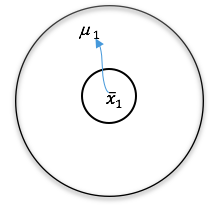
\includegraphics[width=4cm]{chapters/Chapter_12/ext_figure/x1.png} % requires the graphicx package
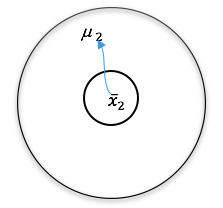
\includegraphics[width=4.3cm]{chapters/Chapter_12/ext_figure/x2.png} % requires the graphicx package
\end{figure}

As you can see, the sample circles including $\bar{x}_1$ and $\bar{x}_2$ are smaller than the entire population circles including $\mu_1$ and $\mu_2$. In other words, we do not have all the information we need to be sure about the exact values of  $\mu_1$ and $\mu_2$. However, as we have learned, statistics allows for sample means to estimate population means as depicted by the arrows. What's new in this chapter is that here we learn statistics can do more than allow us to estimate values for $\mu_1$ and $\mu_2$ separately. We can also use statistics to investigate how the population means differ from one another in tandem. We do this by performing \textit{hypothesis tests} on and using confidence intervals centered around the difference between the sample means $\bar{x}_1$ and $\bar{x}_2$. Let's now turn to some formulaic examples of such tests and intervals.

Is there ``grade inflation'' in WMU?  How does the average GPA of WMU students today compare with, say ten years ago?  Suppose a random sample of 100 student records from 10 years ago yields an average sample GPA of 2.90 with a standard deviation of 0.40.  A random sample of 100 current students today yields a sample average of 2.98 with a standard deviation of 0.45.  The difference between the two-sample means is $2.98 - 2.90 = 0.08$.  Is this proof that GPA's are higher today than ten years ago?  Well $\dots$ first, we need to account for the fact that 2.98 and 2.90 are not the correct averages but that we compute the average from random samples.  Therefore, 0.08 is not the exact difference, but merely an estimate of the actual difference. By how much will it miss?

Note that we took differences $2.98 - 2.90$ to compare average GPA.  The two averages 2.98 and 2.90 are independent, in the sense that we base them on separate and independent groups of students.  The SE of the difference is

\begin{equation}
SE_{(\bar{x}_1 - \bar{x}_2)} = \sqrt{SE_{\bar{x}_1}^2 + SE_{\bar{x}_2}^2 }
\end{equation}

whenever the two means are independent.  Equation (12.1) is similar to the equation from chapter 9, the $SE_{\hat{p}_1 - \hat{p}_2} = \sqrt{(SE_{\hat{p}_1^2} + SE_{\hat{p}_2^2 })}$, for proportions. 

Now, applying the equation from chapter 10, $SE_{\bar{X}}$ which is calculated as $\frac{s}{\sqrt{n}}$ twice, we get

\fbox{\parbox{14cm}{
The standard error of the difference between two independent means.

\begin{equation}
SE_{(\bar{x}_1 - \bar{x}_2)} = \sqrt{\frac{s_1^2}{n_1}  + \frac{s_2^2}{n_2} }
\end{equation}
}}

Continuing with the example, let $\bar{X}_1  = 2.98$ and $\bar{X}_2  = 2.90$.  Then the sample standard deviations are $s_1 = 0.45$ and $s_2 = 0.40$.   The sample sizes are $n_1 = 100$ and $n_2 = 100$.

\begin{equation*}
SE_{(\bar{x}_1 - \bar{x}_2)} = \sqrt{\frac{s_1^2}{n_1}  + \frac{s_2^2}{n_2} } = \sqrt{\frac{0.45^2}{100}  + \frac{0.40^2}{100} } = 0.06
\end{equation*}

Therefore, we can state the conclusion of the study as follows: ``The average GPA of WMU students today is .08 higher than 10 years ago, give or take .06 or so.'' We also could have used equation (12.1) instead of (12.2) in calculating the standard error:

\begin{eqnarray*}
SE_{\bar{X}_1} &=& \frac{s_1}{\sqrt{n_1}} = \frac{0.45}{\sqrt{100}} = 0.045 \\
SE_{\bar{X}_2} &=& \frac{s_2}{\sqrt{n_2}} = \frac{0.40}{\sqrt{100}} = 0.040 \\
SE_{\bar{X}_1 - \bar{X}_2} &=& \sqrt{0.045^2 + 0.040^2} = 0.06 
\end{eqnarray*}

\subsection{Using a confidence interval}

The following two sections discuss the formulas and concepts necessary for calculation and interpretation (respectively) of confidence intervals on the difference between two independent means. Let’s start with the concepts and then proceed to some formulas and examples.

\subsubsection{Confidence Interval - Concepts:}

\begin{figure}[ht]
\centering
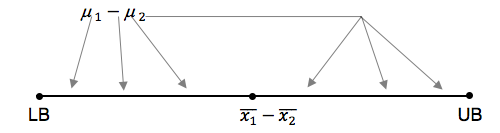
\includegraphics[width=9cm]{chapters/Chapter_12/ext_figure/2sample.png} % requires the graphicx package
\end{figure}

The interval between lower and upper bounds (LB, UB) includes some possible values of $\mu_1 - \mu_2$  (depicted by the many arrows). We need an interval around the central estimate $\bar{x}_1 - \bar{x}_2$ because of variation between samples and populations (which was depicted using concentric circles at the start of this chapter). This interval can be thought of as the ``wiggle room'' needed to estimate $\mu_1 - \mu_2$ using only $\bar{x}_1 - \bar{x}_2$.

Here we show how to use this interval, and it is necessary to talk about some basic properties of a difference first.  For any two numbers A and B, there are three possibilities when evaluating their difference:

\begin{enumerate}
  \item If $A - B$ is a positive number, then A is greater than B. Consider the numbers 4 and 3. If we take $4 - 3 = 1$, the answer is greater than zero.

  \item If $A - B$ is a negative number, then B is higher than A.  For instance if we take  $3 - 4 = -1$, the answer is negative.

  \item If $A - B$ is 0, then A = B. Consider the numbers 4 and 4: $4 - 4 = 0$.
\end{enumerate}

The same kind of reasoning holds for all the possible values of $\mu_1 - \mu_2$ between LB and UB depicted above:

\begin{enumerate}
  \item If all the values from LB to UB are positive, then 
  $\mu_1$ is significantly greater than $\mu_2$.

  \item If all the values from LB to UB are negative, then $\mu_1$ is significantly less than $\mu_2$. 

  \item If zero is between LB and UB (inclusive), then $\mu_1$ is not significantly different from $\mu_2$.
\end{enumerate}

Note that this is to say that the same reasoning and terminology outlined in the section on statistical significance in chapter 9 apply in the new case of a difference.  If the confidence interval for $\mu_1 - \mu_2$ does not contain 0, then 0 has been effectively excluded from the range of possible values.

\fbox{\parbox{14cm}{
When the confidence interval for $\mu_1 - \mu_2$ does not contain \textbf{zero}, we say that the difference is statistically \textbf{significant}.
}}

\subsubsection{Confidence Interval - Calculations and Examples:}

The difference of two means is a random variable with expected value and spread.  The 68\% and 95\% rules apply, i.e. the estimated difference of $\bar{x}_1 - \bar{x}_2$ should be within 1 SE of the true value 68\% of the time, and within 1.96 SE's 95\% of the time.  Following the usual reasoning,    

\begin{equation*}
(\bar{X}_1 - \bar{X}_2) \pm 1.96 SE_{(\bar{X}_1 - \bar{X}_2)}
\end{equation*}

should contain the true difference $(\mu_1 - \mu_2)$ with 95\% confidence.  Substituting (12.2), we get the following formula.

\fbox{\parbox{14cm}{
95\% confidence interval for $(\mu_1 - \mu_2)$:

\begin{equation}
  (\bar{X}_1 - \bar{X}_2) \pm 1.96 \sqrt{\frac{s_1^2}{n_1} + \frac{s_2^2}{n_2}}
\end{equation}
}}

For grade inflation, we have

\begin{equation*}
  (2.98 - 2.90) \pm 1.96 \sqrt{\frac{0.45^2}{100} + \frac{0.40^2}{100}}
\end{equation*}
\begin{equation*}
  0.08 \pm 1.96 (0.06)
\end{equation*}
\begin{equation*}
  (-0.04, 0.20)
\end{equation*}

We say that the difference in GPA averages is between $-.04$ and $.20$ with 95\% confidence.  Note that 0 has not been excluded, making simple chance variability a viable explanation for the observed difference. 

\subsection{Statistical Significance}

Let us revisit the diet study mentioned earlier.  The following table contains the mean changes in body mass index (weight in kilograms divided by height in meters squared) for the Atkins, Zone and Ornish diets. Now, compare the Atkins and Zone diets at 12 months:

\begin{table}[ht]
\centering
\caption{Mean Changes (SD) in Body Mass Index by Diet Group \& Time}
\begin{tabular}{@{} cccc @{}} \hline
Time (months) & Atkins $(n = 77)$ & Zone $(n = 79)$ & Ornish $(n = 76)$ \\ \hline
2 & -1.60(0.98) & -0.76(0.99) & -0.95(0.90) \\
6 & -2.16(2.14) & -0.73(0.90) & -0.85(1.60) \\
12 & -1.65(2.54) & -0.53(2.00) & -0.77(2.14) \\ \hline
\end{tabular}
\end{table}

On the average, Atkins lost how much more body mass index points than Zone?  The estimate of $(\mu_1 - \mu_2)$ is

\begin{equation*}
  (\bar{X}_1 - \bar{X}_2) = (-0.53) - (-1.65) = 1.12
\end{equation*}

The standard error is 

\begin{equation*}
  SE_{(\bar{X}_1 - \bar{X}_2)} = \sqrt{ \frac{(2.00)^2}{79} + \frac{(2.54)^2}{77}} = 0.367
\end{equation*}

The 95\% confidence interval for $(\mu_1 - \mu_2)$ is

\begin{equation*}
  1.12 \pm 1.96 (0.367)
\end{equation*}
\begin{equation*}
(0.84, 1.84)
\end{equation*}

Thus, even allowing for 1.96 SE's of chance variability, Atkins lost at least .40 more body mass index points than Zone (and could be as large as 1.84).   When the confidence interval for $(\mu_1 - \mu_2)$  does not contain zero, we say that the difference is statistically significant.  

\subsection{The P-value}

Continuing the example of the previous section, we might ask ``Can't the difference in averages $\bar{x}_1 - \bar{x}_2 = 1.12$ be explained by chance variability, rather than diet effect?''

The answer is ``Yes, 1.12 can occur by chance, but with very tiny probability.''  How small? Well, if the actual difference were 0, and the SE is 0.367, then the value 1.12 is

\begin{equation*}
\frac{1.12}{0.367} = 3.05
\end{equation*}

SE's from the expected value using the normal curve, random variables fall as far as 3.05 or more SE's from the expected value with approximately 0.0022 probability.  Since this number (also called the $P$-value) is quite small, it makes it hard to believe that the actual difference is zero.  Hence, we conclude that statistically, the two means are different.  Alternatively, we can say that the means are \textit{significantly} different.


\section{Paired data (before-and-after)}

In this section, we will discuss a common problem in data analysis: comparing before and after measurements.  Consider the possible weight loss data in Table 12.2.

\begin{table}[ht]
\centering
\caption{Weight in pounds before and after after 12 months on diet}
\begin{tabular}{@{} crr @{}} \hline
Subject & Before & After \\ \hline
1 & 180 & 155 \\
2 & 192 & 187 \\
3 & 205 & 194 \\
4 & 166 & 176 \\
5 & 220 & 205 \\
6 & 177 & 172 \\
7 & 189 & 173 \\ \hline
Ave: & 189.9 & 180.3 \\
SD:  & 18.1 & 16.4 \\ \hline
\end{tabular}
\end{table}

Using the notation of the previous section estimating the difference between independent means, we have

\begin{center}
\begin{minipage}[ht]{3cm}

$\bar{X}_1 = 189.9$ \\
$s_1 = 18.1$ \\
$n_1 = 7$ 
\end{minipage}
\begin{minipage}[ht]{3cm}

$\bar{X}_2 = 180.3$ \\
$s_2 = 16.4$ \\
$n_2 = 7$ 
\end{minipage}
\end{center}

What is the estimate of mean weight change after 12 months?  $\bar{x}_1 - \bar{x}_2 = 9.6$ pounds, right?  What is the standard error of this estimate? Using equation (12.2) 

\begin{equation*}
SE_{(\bar{x}_1 - \bar{x}_2)} = \sqrt{\frac{s_1^2}{n_1}  + \frac{s_2^2}{n_2} } = \sqrt{\frac{(18.1)^2}{7}  + \frac{(16.4)^2}{7} } = 9.2 \texttt{ pounds}
\end{equation*}

right?  \textbf{wrong!}

We should not use equations (12.1) or (12.2) because the two means are \textbf{not} independent, i.e., they are not calculated on independent samples. The use of the plural `samples' is in itself wrong because we do not have two samples, we only have one! We need to watch out for this.  How many samples are there?  Before-and-after data generally consist of only one sample of subjects, each measured twice.

So how do we calculate an estimate and standard error of average weight loss?  
By calculating the amount of change from Before to After.  The computed value amounts to taking differences, as shown in Table 12.3.

\begin{table}[ht]
\centering
\caption{Weight in pounds before and after after 12 months on diet}
\begin{tabular}{@{} crrr @{}} \hline
Subject & Before & After & Difference \\ \hline
1 & 180 & 155 & 25 \\
2 & 192 & 187 & 5 \\
3 & 205 & 194 & 11 \\
4 & 166 & 176 & -10 \\
5 & 220 & 205 & 15 \\
6 & 177 & 172 & 5 \\
7 & 189 & 173 & 16 \\ \hline
Ave: &  &  & 9.6 \\
SD:  &  & & 11.1 \\ \hline
\end{tabular}
\end{table}

Compare Table 12.3 to Table 12.2.  We have reduced the summary statistics to a single sample, appropriately.  The relevant statistics are now:

$$ \bar{X} = 9.6,  s = 11.1,  n= 7 $$

What does the sample mean $\bar{X} = 9.6$ estimate?  It estimates the average change, right?  To be specific, it estimates the average weight loss from Month 0 to Month 12.  What is the standard error of the estimate?  Since it is just another average, the appropriate procedure is given by 

\begin{equation*}
SE_{\bar{X}} = \frac{s}{\sqrt{n}} = \frac{11.1}{\sqrt{7}} = 4.2 \texttt{ pounds}
\end{equation*}

Completing the analysis, the 95\% confidence interval for average change is

\begin{equation*}
9.6 \pm 1.96 (4.2)
\end{equation*}
\begin{equation*}
(1.4, 17.8)
\end{equation*}

Since the interval does not contain zero, the average weight change is statistically significant.

\subsection{Paired Data}

Paired data are data in which natural matchings occur.  For example, when researchers collect two measurements (one before treatment and one after treatment) from a subject, then we have paired data, and the analysis should follow as described above.  

For example, we might want to compare the head injury of drivers versus passengers in car crashes.   In a study, automobiles were crashed into a wall at a speed of 35 MPH with dummies in the driver and front passenger seat. The head injury criterion (HIC) was measured.  Following is a selection of cars and their HIC values.

\begin{table}[ht]
\centering
\begin{tabular}{@{} lll @{}} \hline
Company & Driver & Passenger \\ \hline
Acura Integra 87        &     		599   &      597 \\
Audi 80 89              &    		600    &     515 \\
Chevrolet Camaro 91     &    		585    &     583 \\
Ford Escort 87          &     		551   &      418 \\
Honda Accord LX 91      &     	562     &    539 \\
Toyota Corolla Fx 88    &    		593     &    397 \\
Volvo 740 GLE 88        &      		519   &      445 \\ \hline
\end{tabular}
\end{table}

Since we uniquely match each pair of observations (e.g., 599 and 597) to each other (driver and passenger HIC in the same car and crash), this is paired data and deserves paired data analysis.

\section{Key Words}

\fbox{\parbox{14cm}{
\begin{minipage}[ht]{6cm}

\begin{itemize}
\item independent sample \\ experiment
\item paired difference experiment
\end{itemize}
\end{minipage} \hfill
\begin{minipage}[ht]{6cm}

\begin{itemize}
\item confidence intervals
\item sampling distribution
\end{itemize}
\end{minipage}
}}

\twocolumn

\section{}

\begin{exercises}
\begin{exercise} % 1

Do credit cards with no annual fee charge higher interest rates (APR) than cards that have annual fees?  Among 29 cards surveyed, 17 had no annual fees while 12 charged an annual fee.  Among the cards with no annual fee, the average APR was 19\% (SD=8\%).  Among cards with an annual fee, the average APR was 17\% (SD=3\%).

\begin{enumerate}
  \item Estimate the difference in APR.
  \item Calculate a standard error for your estimate in (1).
  \item Calculate a 95\% confidence interval for the difference in APR between the two groups.
  \item Are interest rates significantly higher \\ for cards with no annual fees?
  \item What is the P-value for comparing the two averages? Is the difference significant?
\end{enumerate}
\end{exercise}
\begin{solution} % 1


\end{solution}

\begin{exercise}  % 2

100 students graduating \\ with Bachelor degrees in engineering make an average of \$70,000 with a standard deviation of \$5,000 when entering the workforce. 68 students graduating with Bachelor \\ degrees in statistics make an average of \\ \$65,000 with a standard deviation of \$3,000 when entering the workforce. Assuming the two samples of students are independent, answer the following questions:

\begin{enumerate}
  \item What is the difference between the \\ sample averages (engineers – \\ statisticians)?
  \item What is the standard error of the estimate for the true difference in average entrance salaries between all engineering and statistics BA graduates?
  \item What is a 95\% confidence interval for the difference in sample averages?
  \item Do these statistics suggest that average entrance salaries for stats vs. engineering students are significantly different?
\end{enumerate}

\end{exercise}
\begin{solution}  % 2

\end{solution}

\begin{exercise}  % 3

A Junior at Southwest \\ Michigan college is debating whether to pursue an MBA after her Bachelor degree in \\ management.  She interviews some people \\ she  knows in the workforce and was able to obtain their salaries. The annual salaries (in dollars) are summarized in the following table:

\begin{tabular}{@{} lccc @{}} \hline
Degree & Aver & SD & Sample Size \\ \hline
Bachelor & \$48,286 & \$416 & 12 \\
Master   & \$59,496 & \$675 & 7 \\ \hline
\end{tabular}

\begin{enumerate}
  \item Estimate the difference in average \\ salary between the two groups.
  \item Calculate a standard error for our estimate in (1).
  \item Calculate a 95\% confidence interval for the average difference in salary.
  \item Are MBA salaries significantly higher?
  \item What is the P-value for comparing the two averages? Is the difference significant?
\end{enumerate}
\end{exercise}  
\begin{solution}  % 3

\end{solution}

\begin{exercise}  % 4

A group of charity \\ workers employed by a large foundation \\ track the donations made to the foundation every  month. They note that the average donations for August were somewhat higher \\ than the average donations for September, \\ and they want to know if this fact should \\ worry them moving forward. Performing the correct statistical test could determine \\ whether the average difference in donations between  August and  September was significant. However, they  must first decide \\ whether their August and  September donations are independent or not. If we were advising the charity workers, what would we tell them?
\end{exercise}
\begin{solution}  % 4


\end{solution}

\begin{exercise}  % 5

A new gasoline \\ additive is supposed to make gas burn more cleanly and increase gas mileage in the process.  \\ Consumer Protection Anonymous conducted a mileage test to confirm this.  They took \\ seven of their cars, filled it with regular gas, and drove it on I-94 until it was empty.  They repeated the process using the same cars, but using the gas additive.  The recorded gas \\ mileage follows:

{\footnotesize{
\begin{tabular}{@{} llllllll @{}} \hline
Additive & 1 & 2 & 3 & 4 & 5 & 6 & 7 \\ \hline
Without & 22 & 15 & 18 & 28 & 12 & 25 & 18 \\
With    & 26 & 19 & 17 & 34 & 17 & 25 & 22 \\ \hline
\end{tabular}
}}

\begin{enumerate}
  \item Calculate the mean difference in \\ mileage between the two fuel types.         \item Calculate a standard error for our estimate in (1).
  \item Calculate a 95\% confidence interval for the mean \\ mileage difference.
  \item Does the data support the claim of \\ higher gas mileage?
\end{enumerate}

\end{exercise}
\begin{solution}  % 5

\end{solution}

\begin{exercise}  % 6

The group of charity \\ workers from the above question decides on a statistical test based on the sage wisdom we previously offered. They perform a test for significance of the average difference, and it yields a p-value of 0.50. As their stats advisor, how would we interpret this p-value concerning  whether the average difference in donations for August versus September was \\ significant?
\end{exercise}
\begin{solution}  % 6

\end{solution}

\begin{exercise}  % 7

Suppose a shoe \\ company wants to test material for the soles of shoes.  For each pair of shoes the new material is placed on one shoe and the old material is placed on the other shoe.  After a given period of time a random sample of 16 pairs of shoes is selected.  The wear is measured on a 10 point scale (higher is better) with the following results.  The average of the differences is $\bar{X}_n - \bar{X}_o = 0.4$ and it standard deviation is $s_{diff} = 1.6$.

\begin{enumerate}
  \item Determine the mean difference in the sole-wear between the two material \\ types.        
  \item Calculate a standard error for our estimate in (1).
  \item Calculate a 95\% confidence interval for the mean sole-wear difference.
  \item Does the data support the claim that the new material gives superior wear?
\end{enumerate}

\end{exercise}
\begin{solution}  % # 7



\begin{enumerate}
  \item $\bar{X}_d = 0.4 $     
  \item $SE_d = 0.4$
  \item $95\% CI  \rightarrow ( -0.4525798, 1.2525798 )$
  \item Does the data support the claim that the new material gives superior wear?  No, since zero is contained in the 95\% CI.
\end{enumerate}

\end{solution}

\begin{exercise}   % 8

% latex table generated in R 4.0.2 by xtable 1.8-4 package
% Fri Jul 31 12:47:41 2020
\begin{table}[ht]
\centering
\begin{tabular}{rll}
  \hline
 & RMon & RMoff \\ 
  \hline
Mean & 40.67 & 34.53 \\ 
  SD & 10.040 & 9.561 \\ 
  n & 15 & 15 \\ 
   \hline
\end{tabular}
\caption{Ramp Metering} 
\end{table}


Ramp metering is an \\ engineering experiment that studies how automobiles enter an expressway to stop for a \\ short time before they join the flow of traffic.  The theory is that ramp metering  directs the number of vehicles on the expressway and the  number of vehicles accessing the expressway, resulting in a freer flow, which results in a faster travel times.  To prove the hypothesis whether ramp metering affects travel time, traffic engineers in Kalamazoo, Michigan, set up an experiment on a section of expressway where ramp meters were installed.  The response variable was the speed of vehicles.  A random sample of 15 vehicles on the expressway for a Tuesday at 5 p.m. with the ramp meters on and a second random sample of 15 vehicles on a different Tuesday at 5 p.m. with the ramp meters off resulted in the following speed summaries(in miles per hour).

\begin{enumerate}
  \item Determine the mean difference \\ between ramp meters on and ramp meters off.
  \item Calculate a standard error for our estimate in (1).
  \item Calculate a 95\% confidence interval for the mean ramp meter on-off difference.
  \item Does the data support the claim that ramp metering improves traffic flow?
\end{enumerate}


\end{exercise}
\begin{solution}  % 8


\end{solution}


\end{exercises}


\onecolumn











%!Rnw root = ../../Main.Rnw

\chapter{More Comparing Two Means}
\label{chap:ch13}

\section{Objectives}

After completing this part, students should be able to:

\fbox{\parbox{14cm}{
\begin{itemize}
\item Set-up and perform hypothesis testing for means
\item Explain Type I and Type II errors
\item Articulate the conclusions to a broader audience.
\end{itemize}
}}

\section{Overview and Example 1}

\subsection{Grade Inflation Revisited}

The previous chapter outlines a situation where some grade inflation might occur at WMU over the last ten years.  The method used to analyze this situation was a confidence interval.  Instead of a confidence interval, let us return to that example, and try a different form of analysis:  the hypothesis test using test statistic, and $p$-value.  The new method will have the same result as the confidence interval.  However, we must learn both methods since many disciplines use both statistical analyses.  Let us review the relevant statistics.

Suppose a random sample of 100 student records from 10 years ago yields an average sample GPA of 2.90 with a standard deviation of 0.40. A random sample of 100 current students today yields a sample average of 2.98 with a standard deviation of 0.45. The difference between the two-sample means is $2.98 - 2.90 = 0.08$.  We will use the following  notation: $n_1 = 100$, $\bar{x}_1 = 2.90$, $s_1 = 0.40$, $n_2 = 100$, $\bar{x}_2 = 2.98$, and $s_2 = 0.45$.

% \newpage

What are the two possibilities here?


\begin{enumerate}
\item There is no grade inflation at WMU, our sample is in error.
\item There is grade inflation at WMU, our sample is not in error.
\end{enumerate}


Although we cannot say for sure which of the possibilities is true, we can calculate the probability of each possibility. To do so, we will (as always) assume the normal distribution holds, assume the two means are independent, calculate a standard error, calculate a test statistic, and find a $p$-value.

\subsection{Define Hypotheses Testing}

Definition: Hypotheses testing is a process of using sample data and probability to test the characteristics of one or more populations. In the present example, the populations are all the students at WMU during the first sampling, and all students at WMU during the second sampling.

Here is how we use hypotheses tests:

\begin{enumerate}
\item Make a statement about the nature of the population(s). 
\item Formulate an Analysis Plan.
  \begin{itemize}
  \item Sampling Distribution is approximately normal 
  \item Choose a level of significance equal to 0.05.
  \item Decide the number of observations.
  \item Select a test method.
  \end{itemize}
\item Analyze the data.
\item Interpret the Results.
\item Communicate our results to the audience.
\end{enumerate}

\subsubsection{Definition:} The Null Hypothesis $(H_0)$ is a statement about the status quo. It says there is no difference.

\subsubsection{Definition:} The Alternative Hypothesis $(H_a)$ is a statement that contradicts the $(H_0)$. It says there is a difference.

If the null hypothesis is true, then in a sense nothing special is going on. In the present example, the null hypothesis is that there is no grade inflation at WMU. Can we reject this null hypothesis and state that it is probably the case that there is grade inflation at WMU? If so, then we would be affirming the alternative hypothesis We will find out soon. For now let us write that:

\begin{eqnarray*}
H_0: \mu_1 = \mu_2 \\
H_a: \mu_1 \ne \mu_2 
\end{eqnarray*}

The greek letter $\mu$ is a common symbol for a population mean. This is convenient notation that really says the same thing as the above text: the null hypothesis is that the two population means are equal, or that there is no difference between WMU grades at time 1 and time 2; the alternative hypothesis is that the two population means are not equal, or that there is a difference between WMU grades at time 1 and time 2. Often in the real world of statistical analyses, the statement of the alternative hypothesis is a little more difficult. An alternative hypothesis could be $<$, $>$, or $\ne$, i.e., it could be either one or two-tailed, but in our course we keep things simple for you and simply always use $\ne$.

\section{Calculation and Analysis for Example 1}

When the difference, between the observed means of sample A and sample B, is similar; we can expect no significance, i.e., $(\bar{x}_1 - \bar{x}_2) \sim 0 $.   On the other hand, when the means are
dissimilar, we should expect a significant difference. The bigger the difference, the more likely we are to find significance and conclude with the alternative hypothesis. Recalling that our difference in the grade inflation example is $(2.98 - 2.90) = 0.08$, we might expect there really is not a significant difference here, but let us perform the full analysis to find out.

\begin{enumerate}
\item State the hypotheses
  \begin{itemize}
  \item $H_0: \mu_1 = \mu_2$ ,  there is no grade inflation. 
  \item $H_a: \mu_1 \ne \mu_2$ ,  there is  grade inflation. 
  \end{itemize}
\item Formulate an Analysis Plan:
  \begin{enumerate}
  \item We assume the sampling Distribution is approximately normal
  \item Choose a level of significance equal to 0.05 (this could be any value $\le 1$,  but again, we will keep things simple for this course and always select 0.05 or 95 percent confidence).
  \item Determine the number of observations: $n_1 = 100, n_2 = 100$. 
  \item Selecting a standard error based on the above assumptions:
  
  \begin{eqnarray*}
  SE_{\bar{x}_1 - \bar{x}_2} &=& \sqrt{ SE_{\bar{x}_1} + SE_{\bar{x}_2}} \\
   &=& \sqrt{ \frac{s_1^2}{n_1} + \frac{s_2^2}{n_2}}
   \end{eqnarray*} 
 
\item Selecting a test method (statistic):

  \begin{eqnarray*}
  Z_0 &=& \frac{ \bar{x}_1 - \bar{x}_2}{SE_{\bar{x}_1 - \bar{x}_2}} \\
  &=& \frac{ \bar{x}_1 - \bar{x}_2}{ \sqrt{ \frac{s_1^2}{n_1} + \frac{s_2^2}{n_2}} }
   \end{eqnarray*} 
 \end{enumerate}
 
\item Analyze the data. Let us calculate the above:

  \begin{eqnarray*}
  Z_0 &=& \frac{ \bar{x}_1 - \bar{x}_2}{ \sqrt{ \frac{s_1^2}{n_1} + \frac{s_2^2}{n_2}} } \\
    &=& \frac{ 2.98 - 2.90 }{ \sqrt{ \frac{0.45^2 }{100} + \frac{0.40^2}{100}}} \\
    &=& \frac{ 0.08}{0.06} \\
    &\approx& 1.3333 
   \end{eqnarray*} 
   
\item Interpret the Results.

\begin{itemize}
\item The test statistic is relatively small at $Z_0 = 1.3333$.  Recall that we decided on a significance level $(\alpha)$ of 0.05. This level of significance implies we’d need at least $|Z| = 1.96$ to conclude there is a significant change between the two sampling times.

\item We cannot conclude a significant difference, so we do not reject the null hypothesis. Our sample does not show there is significant grade inflation at WMU.

\item Note: We have to be careful here. This is not quite the same as saying there is no grade inflation at WMU. Instead, we say that it’s not likely there is grade inflation given our sample data. We just don’t have enough evidence for the alternative hypothesis that there is grade inflation.

\item Could we have used the $p$-value instead to decide whether to reject the null hypothesis? Yes. The $p$-value of these two-tailed tests is the probability of obtaining an $|Z|$ value larger than that of the test statistic.  In notation: 
$p$-value $ = P[ |Z| > |Z_0|$].  This probability can be obtained from the $Z$-table by finding the area of the curve less than a negative $Z_0$ or greater than a positive $Z_0$, then multiplying this area by 2. In our example, the probability obtained from the $Z$-table using $Z_0 = 1.33$ is 0.0918.  $p$-value $= 2 \times 0.0918 = 0.1836$. Recall now that our significance level was set at 0.05 at the outset of this problem.  We use the decision rule that the $p$-value must be less or equal to the significance level in order to reject the null hypothesis. 
Since our $p$-value 0.1836 is much greater than 0.05, therefore, we do not reject the null hypothesis (as we expected). Once again we conclude there is not enough evidence to decide there is grade inflation at WMU, whether using the test statistic, the $p$-value, or the previous chapter confidence interval.

\end{itemize}

\end{enumerate}

\section{Example 2}

\subsection{The Question}

In their paper \textit{Modeling wine preferences by data mining from physicochemical properties,} \footnote{ P. Cortez, A. Cerdeira, F. Almeida, T. Matos and J. Reis. Modeling wine preferences by data mining from physicochemical properties.  In Decision Support Systems, Elsevier, 47(4):547-553, 2009.}
Cortez et al. present a dataset on wine qualities and preferences. Many interesting variables
are included such as the pH, fixed acidity, alcohol content, and quality score for thousands of 
sampled wines. For the remainder of this chapter, we will use this dataset to compare means 


So what questions can we ask about the wines using this dataset? There are many interesting topics to choose from since the dataset contains 13 variables across 6497 different sampled wines. Let’s start with grouping by color and go from there; the dataset contains 1599 red wines and 4898 white wines. Do you think there may be a difference in the fixed acidity of red vs. white wines? Let’s find out.

\subsubsection{The Question:}  Do the averages of fixed acidity for white vs. red wines significantly differ?

\subsection{Working Through Example 2}



\begin{enumerate}
\item Make a statement about the nature of the population(s).

We did this above. Let’s note here that the two populations, red vs. white wines, are independent of one another as required by the mathematics taught here.

\item Formulate an Analysis Plan.

  \begin{itemize}
  \item Sampling Distribution is approximately normal \\ Are the samples roughly normal? Let’s check by constructing histograms:
  
\begin{minipage}[ht]{6cm}



{\centering \includegraphics[width=6cm,height=6cm]{figure/LBL13ab-1} 

}




\end{minipage}
\begin{minipage}[ht]{6cm}



{\centering \includegraphics[width=6cm,height=6cm]{figure/LBL13ac-1} 

}



\end{minipage}


Although a little right skewed, we can treat these as normal for our purposes. It is always a good idea to check the data before proceeding. We also know the samples are separate.

  \item Choose a level of significance equal to 0.05.

  Recall this implies that we'll use a benchmark $|Z| = 1.96$ to draw our conclusions at the end.
  
  \item Determine the number of observations.
  
  As noted above, there are 6497 different sampled wines in this dataset. 1599 are
red, and 4898 are white.

  \item Select a test method.
  
  We'll use the same $Z_0$ as before:
  
    \begin{eqnarray*}
    Z_0 &=& \frac{ \bar{x}_1 - \bar{x}_2}{SE_{\bar{x}_1 - \bar{x}_2}} \\
      &=& \frac{ \bar{x}_1 - \bar{x}_2}{ \sqrt{ \frac{s_1^2}{n_1} + \frac{s_2^2}{n_2}} }
   \end{eqnarray*} 

  \end{itemize}
  
\item Analyze the data.

  \begin{itemize}
  \item $H_0: \mu_w = \mu_r$ ,    there is no difference in fixed acidity between red and white wines. 
  \item $H_a: \mu_w \ne \mu_r$ ,  there is a difference in fixed acidity between red and white wines. 
  \end{itemize}
  
  We will use R software to calculate the necessary sample statistic:
 
 % Requires the booktabs if the memoir class is not being used
\begin{table}[htbp]
   \centering
   \caption{Summary Statistics}
   %\topcaption{Table captions are better up top} % requires the topcapt package
   \begin{tabular}{@{} lrr @{}}  \hline % Column formatting, @{} suppresses leading/trailing space
      % \toprule
      & \multicolumn{2}{c}{Wines } \\
      \hline 
      % \cmidrule(r){1-2} % Partial rule. (r) trims the line a little bit on the right; (l) & (lr) also possible
          & White(w)  & Red(r)  \\ \hline
      % \midrule
      Mean & 6.8547877 & 8.3196373 \\
      SD   & 0.8438682 & 1.7410963 \\
      N    & 4898  & 1599  \\ \hline
   \end{tabular}
   
   \label{tab:tbwines}
\end{table} 

Finally we calculate the test statistic:

  \begin{eqnarray*}
  Z_0 &=& \frac{ \bar{x}_w - \bar{x}_r}{ \sqrt{ \frac{s_w^2}{n_w} + \frac{s_r^2}{n_r}}} \\
    &=& \frac{ 6.85 - 8.32 }{ \sqrt{ \frac{0.844^2 }{4898} + \frac{1.741^2}{1599}}} \\
    &\approx& -32.42 
   \end{eqnarray*} 
   
Note that this time we obtained a negative $Z_0$ because of the way we took the difference in the numerator. There is nothing wrong with this. We could have switched the numerator around and obtained its positive counterpart just as easily.

\item Interpret the Results.

This $Z_0 = -32.42$ is an extreme Z value.  It falls very far off the Z table.  This is much less than $Z = -1.96$, so we reject the null hypothesis with great force.  We might also consider the $p$-value. Although the $p$-value cannot be obtained from the Z-table since it does not go beyond -4, we can use R software to calculate it. The $p$-value is 1.43e-230, diminishingly smaller than 0.05, so we reject the null hypothesis. The fixed acidities are quite different given the large sample size. We are much more than 95 percent confident that white wine and red wine differ in their fixed acidities according to this analysis.

\item Communicate our results to the audience.

Many different options are available to you here such as the histograms, sample statistics, test statistic, and $p$-value.  Perhaps the most difficult point to make is the significance of our $Z_0$ since it is quite far from zero, and the $p$-value quite small. To help with this, we can say we are over 30 standard errors from no difference between these two means! We could also say that the $p$-value has over 200 zeros past the decimal!

\end{enumerate}

\subsection{Large Samples, Free Data, and Free Software }

The wine dataset used above is freely available online and fun to play with. One reason it was selected for this chapter was to demonstrate the impact a larger sample can have on your analysis. As you saw above, a large sample tends to make even small differences appear extremely significant. Another reason it was selected was to demonstrate the computational power you can get out of the free R software used to do the calculations. The reader is highly encouraged to download both the dataset and R software to do some explorations of their own. Please do not hesitate to ask your instructor for help downloading or using R during your coursework with us.

\section{Key Words}

\fbox{\parbox{14cm}{
\begin{minipage}[ht]{6cm}

\begin{itemize}
\item Dependent
\item Independent
\item Sampling Distribution 
\item Normal Distribution
\item Hypothesis Testing
\item Null Hypothesis
\end{itemize}
\end{minipage} \hfill
\begin{minipage}[ht]{6cm}

\begin{itemize}
\item Alternative Hypothesis 
\item Standard Error
\item Test Statistic
\item P-value
\item Significance Level
\item Two Sample Means
\end{itemize}
\end{minipage}
}}

\twocolumn

\section{}

\begin{exercises}
\begin{exercise} % 1



The wine quality \\ dataset used in this chapter includes a variable on alcohol content. The average alcohol content of red wine is 10.423, while that of white wine is 10.5143. The respective standard deviations are 1.0657 and 1.2306. The respective sample sizes are 1599 and 4898.

\begin{itemize}
  \item Set up a hypothesis test. What are the two hypotheses?
  \item What is the difference between means?
  \item What is the standard error of the difference?
  \item What is the test statistic $Z_0$?
  \item What is the $p$-value?
  \item What should you conclude?
\end{itemize}

\end{exercise}
\begin{solution} % 1

Percent of alcohol 

\begin{itemize}
  \item $H_0: \mu_r = \mu_w$ vs. $H_a: \mu_r \ne \mu_w$
  \item  means difference = -0.0912839
  \item  standard error  = 0.0319283
  \item  test statistic = -2.8590288
  \item  $p$-value = 0.0042494
  \item  I conclude to reject the null hypothesis since the p-value is less than 0.05.
\end{itemize}

\end{solution}

\begin{exercise} % 2

The wine quality \\ dataset used in this chapter includes a variable on quality. The average quality score of red wine is 5.636, while that of white wine is 5.8779. The respective standard deviations are \\ 0.8076 and 0.8856. The respective sample sizes are 1599 and 4898.

\begin{itemize}
  \item Set up a hypothesis test. What are the two hypotheses?
  \item What is the difference between means?
  \item What is the standard error of the difference?
  \item What is the test statistic $Z_0$?
  \item What is the $p$-value?
  \item What should you conclude?
\end{itemize}

\end{exercise}
% \begin{solution} % 2
% 
% 
% \end{solution}

\begin{exercise} % 3

True or False? Suppose a two-tailed $Z_0$ test statistic is calculated and it is positive. Then the $p$-value will be the area below this $Z_0$.

\end{exercise}
\begin{solution} % 3

False

\end{solution}

\begin{exercise} % 4

True or False? Suppose a two-tailed $Z_0$ test statistic is calculated and it is negative. Then the $p$-value will be the area below this $Z_0$.

\end{exercise}
% \begin{solution} % 4
% 
% 
% \end{solution}

\begin{exercise} % 5

True or False? If we obtain a test statistic that is either much greater than 1.96 or much smaller than -1.96, then we fail to reject the null hypothesis.

\end{exercise}
\begin{solution} % 5

False 

\end{solution}


\begin{exercise} % 6

True or False? If we obtain a $p$-value that is much larger than 0.05, then we fail to reject the null hypothesis.

\end{exercise}
% \begin{solution} % 6
% 
% 
% \end{solution}

\begin{exercise}  % 7



100 students graduating \\ with Bachelor degrees in engineering make an average of \$70,000 with a standard deviation of \$5,000 when entering the workforce. 68 students graduating with Bachelor \\ degrees in statistics make an average of \\  \$65,000 with a standard deviation of \$3,000 when entering the workforce. Assuming the two samples of students are independent, answer the following questions:

\begin{itemize}
  \item Set up a hypothesis test. What are the two hypotheses?
  \item What is the difference between means?
  \item What is the standard error of the difference?
  \item What is the test statistic $Z_0$?
  \item What is the $p$-value?
  \item What should you conclude?
\end{itemize}

\end{exercise}
\begin{solution}  % 7

\begin{itemize}
  \item $H_0: \mu_e = \mu_s$ vs. $H_a: \mu_e \ne \mu_s$
  \item  means difference = 5000
  \item  standard error  = 618.3469424
  \item  test statistic = 8.0860754
  \item  $p$-value = 0.0042494
  \item  I conclude to reject the null hypothesis since the p-value is greater than 0.05.
\end{itemize}

\end{solution}


% \begin{exercise} % 1
% 
% Do credit cards with no annual fee charge higher interest rates (APR) than cards that have annual fees?  Among 29 cards surveyed, 17 had no annual fees while 12 charged an annual fee.  Among the cards with no annual fee, the average APR was 19\% (SD=8\%).  Among cards with an annual fee, the average APR was 17\% (SD=3\%).
% 
% \begin{enumerate}
%   \item Estimate the difference in APR.
%   \item Calculate a standard error for your estimate in (1).
%   \item Calculate a 95\% confidence interval for the difference in APR between the two groups.
%   \item Are interest rates significantly higher for cards with no annual fees?
%   \item What is the P-value for comparing the two averages? Is the difference significant?
% \end{enumerate}
% \end{exercise}
% \begin{solution} % 1
% 
% 
% \end{solution}
%
% 
% \begin{exercise}  % 3
% 
% A Junior at Southwest \\ Michigan college is debating whether to pursue an MBA after her Bachelor degree in management.  She interviews some people she \\ knows in the workforce and was able to obtain their salaries. The annual salaries (in dollars) are summarized in the following table:
% 
% \begin{tabular}{@{} lccc @{}} \hline
% Degree & Aver & SD & Sample Size \\ \hline
% Bachelor & \$48,286 & \$416 & 12 \\
% Master   & \$59,496 & \$675 & 7 \\ \hline
% \end{tabular}
% 
% \begin{enumerate}
%   \item Estimate the difference in average salary between the two groups.
%   \item Calculate a standard error for our estimate in (1).
%   \item Calculate a 95\% confidence interval for the average difference in salary.
%   \item Are MBA salaries significantly higher?
%   \item What is the P-value for comparing the two averages? Is the difference significant?
% \end{enumerate}
% \end{exercise}  
% \begin{solution}  % 3
% 
% \end{solution}
% 
% \begin{exercise}  % 4
% 
% A group of charity workers employed by a large foundation track the donations made to the foundation every month. They note that the average donations for August were somewhat higher than the average donations for September, and they want to know if this fact should worry them moving forward. Performing the correct statistical test could determine whether the average difference in donations between August and \\ September was significant. However, they \\ must first decide whether their August and  September donations are independent or not. If we were advising the charity workers, what would we tell them?
% \end{exercise}
% \begin{solution}  % 4
% 
% 
% \end{solution}
% 
% \begin{exercise}  % 5
% 
% A new gasoline additive is supposed to make gas burn more cleanly and increase gas mileage in the process.  Consumer Protection Anonymous conducted a mileage test to confirm this.  They took seven of their cars, filled it with regular gas, and drove it on I-94 until it was empty.  They repeated the process using the same cars, but using the gas additive.  The recorded gas mileage follows:
% 
% \begin{tabular}{@{} llllllll @{}} \hline
% Additive & 1 & 2 & 3 & 4 & 5 & 6 & 7 \\ \hline
% Without & 22 & 15 & 18 & 28 & 12 & 25 & 18 \\
% With    & 26 & 19 & 17 & 34 & 17 & 25 & 22 \\ \hline
% \end{tabular}
% 
% \begin{enumerate}
%   \item Calculate the mean difference in mileage between the two fuel types.         \item Calculate a standard error for our estimate in (1).
%   \item Calculate a 95\% confidence interval for the mean mileage difference.
%   \item Does the data support the claim of \\ higher gas mileage?
% \end{enumerate}
% 
% \end{exercise}
% \begin{solution}  % 5
% 
% \end{solution}
% 
% \begin{exercise}  % 6
% 
% The group of charity workers from the above question decides on a statistical test based on the sage wisdom we previously offered. They perform a test for significance of the average difference, and it yields a p-value of 0.50. As their stats advisor, how would we interpret this p-value concerning \\ whether the average difference in donations for August versus September was \\ significant?
% \end{exercise}
% \begin{solution}  % 6
% 
% \end{solution}
% 
% \begin{exercise}  % 7
% 
% Suppose a shoe company wants to test material for the soles of shoes.  For each pair of shoes the new material is placed on one shoe and the old material is placed on the other shoe.  After a given period of time a random sample of 16 pairs of shoes is selected.  The wear is measured on a 10 point scale (higher is better) with the following results.  The average of the differences is $\bar{X}_n - \bar{X}_o = 0.4$ and it standard deviation is $s_{diff} = 1.6$.
% 
% \begin{enumerate}
%   \item Determine the mean difference in the sole-wear between the two material \\ types.        
%   \item Calculate a standard error for our estimate in (1).
%   \item Calculate a 95\% confidence interval for the mean sole-wear difference.
%   \item Does the data support the claim that the new material gives superior wear?
% \end{enumerate}
% 
% \end{exercise}
% \begin{solution}  % # 7
% 
% <<label=LBL13a, results="asis", echo=FALSE>>=
%   n11 <- 16
%   xbar11 <- 0.4
%   sd11 <- 1.6
%   se11 <- 1.6 / sqrt(16)
%   cv11 <- qt(.975, (n11-1))
%   lbnd11 <- xbar11 - cv11 * se11
%   ubnd11 <- xbar11 + cv11 * se11
% @
% 
% \begin{enumerate}
%   \item $\bar{X}_d = xbar11 $     
%   \item $SE_d = se11$
%   \item $95\% CI  \rightarrow ( lbnd11, ubnd11 )$
%   \item Does the data support the claim that the new material gives superior wear?  No, since zero is contained in the 95\% CI.
% \end{enumerate}
% 
% \end{solution}
% 
% \begin{exercise}   % 8
% 
% <<label=LBL13b, results="asis", echo=FALSE>>=
%   RMon  <- c(28,38,43,35,42,48,31,46,55,26,56,25,50,40,47)
%   RMoff <- c(24,34,47,29,37,26,37,38,23,52,42,31,17,40,41)
%   tbl1 <- matrix(nrow=3,ncol=2)
%   rownames(tbl1)<- c('Mean', 'SD', 'n')
%   colnames(tbl1)<- c('RMon', 'RMoff')
%   tmp11 <- mean(RMon)
%   tbl1[1,1] <- sprintf("%.2f",tmp11)
%   tmp21 <- sd(RMon)
%   tbl1[2,1] <- sprintf("%.3f", tmp21)
%   tmp31 <- length(RMon)
%   tbl1[3,1] <- sprintf("%.0f", tmp31)
%   tmp12 <- mean(RMoff)
%   tbl1[1,2] <- sprintf("%.2f", tmp12)
%   tmp22 <- sd(RMoff)
%   tbl1[2,2] <- sprintf("%.3f", tmp22)
%   tmp32 <- length(RMoff)
%   tbl1[3,2] <- sprintf("%.0f", tmp32)
%   
%   diff1 <- tmp11 - tmp12
%   SE1   <- sqrt( (tmp21^2/tmp31) + (tmp22^2/tmp32 ))
%   z1    <- diff1/ SE1
%   pval1 <- 1 - pnorm(z1)
%   xtable(tbl1, caption="Ramp Metering")
%                  
% @  
% 
% Ramp metering is an engineering experiment that studies how automobiles enter an expressway to stop for a short time before they join the flow of traffic.  The theory is that ramp metering  directs the number of vehicles on the expressway and the \\ number of vehicles accessing the expressway, resulting in a freer flow, which results in a faster travel times.  To prove the hypothesis whether ramp metering affects travel time, traffic engineers in Kalamazoo, Michigan, set up an experiment on a section of expressway where ramp meters were installed.  The response variable was the speed of vehicles.  A random sample of 15 vehicles on the expressway for a Tuesday at 5 p.m. with the ramp meters on and a second random sample of 15 vehicles on a different Tuesday at 5 p.m. with the ramp meters off resulted in the following speed summaries(in miles per hour).
% 
% \begin{enumerate}
%   \item Determine the mean difference between ramp meters on and ramp meters off.
%           
%   \item Calculate a standard error for our estimate in (1).
%   \item Calculate a 95\% confidence interval for the mean ramp meter on-off difference.
%   \item Does the data support the claim that ramp metering improves traffic flow?
% \end{enumerate}
% 
% 
% \end{exercise}
% \begin{solution}  % 8
% 
% 
% \end{solution}


\end{exercises}


\onecolumn











%!Rnw root = ../../Main.Rnw

\chapter{Categorical Variables: Association or Independence}
\label{chap:ch14}

\section{Objectives}

After completing this part, students should be able to:

\fbox{\parbox{14cm}{
\begin{itemize}
\item Compute expected frequencies.
\item Understand the difference between association and independence.
\item Test for a statistical association.
\end{itemize}

}}

\section{Association versus independence in an r x c table}  \index{association}

Is there an association between gender and height?  Yes, males tend to be taller than females.  A more formal way of saying this is `height distribution for males tends to be different from females.'   Is there an association between shoe size and height?  Yes,  `height distribution for men who wear size 12 is different from those who wear size 8.'    Is there an association between GPA and height?  No, `height distribution tends to be the same for 3.0 students as well as 3.5 students.'

\fbox{\parbox{14cm}{
Two variables A and B are said to be \textbf{associated} if the distribution of B tends to change with the level of the A variable.  Otherwise, they are said to be \textbf{independent} variables. 
}}

Therefore, height is associated with gender and shoe size, but independent of GPA.  

If we are thinking, ``association and independence are the same,''  we are almost correct.  The difference is about design. In the test of independence, we collect observational units at random from a population, and the two categorical variables are observed for each unit. In the test of association, we collect the data by randomly sampling from each sub-group \textbf{separately}. (Say, 100 Democrat, 100 Republican, 100 Independent, and so on.) The null hypothesis is that each sub-group shares the same distribution of another categorical variable. (Say, ``chain smoker'', ``occasional smoker'', ``non-smoker''.)  The difference between these two tests is subtle yet important.

Now consider the following 3 by 4 table.  Researchers followed 189 students entering a business school program as part of attrition (i.e., drop out, transfer) study.  The students were cross-classified according to 4 categories of high school GPA $(2.0-2.5, 2.5-3.0, 3.0-3.5, 3.5-4.0)$ and three categories of attrition outcomes (`did not return for the 2nd year,' `returned for second but not for a 3rd year,' `returned for 3rd year').  Is there an association between HS GPA and college attrition?

\begin{table}[ht]
\centering
\caption{Retention versus HS GPA}
\begin{tabular}{@{} lcccc @{}} \hline
& \multicolumn{4}{c}{GPA} \\
Returned & $2.0-2.5$ & $2.5-3.0$ & $3.0-3.5$ & $3.5-4.0$ \\ \hline
No --2nd yr & 25 & 3 & 4 & 6 \\
No -- 3rd yr & 14 & 7 & 4 & 6 \\
Yes -- 3rd yr & 41 & 7 & 28 & 44 \\ \hline
\end{tabular}
\end{table}

To analyze whether attrition and GPA are independent, we will analyze whether attrition distribution remains the same regardless of GPA level.  Let us start by looking at the 1st column (worst HS grades) and 4th column (best HS grades).  Do the distributions look the same?   The answer seems to be `no' - a bigger proportion of the 1st column never returned for their second year.  In other words, the value `25' in the very first cell is too large, implying that 'poor grades seems to be associated with first-year attrition.'  If grades and attrition were independent, Table 14.1 should have looked more like Table 14.2.

\begin{table}[ht]
\centering
\caption{Expected counts (if independent)}
\begin{tabular}{@{} lcccc @{}} \hline
& \multicolumn{4}{c}{GPA} \\
Returned & $2.0-2.5$ & $2.5-3.0$ & $3.0-3.5$ & $3.5-4.0$ \\ \hline
No --2nd yr & 16 & 3 & 7 & 11 \\
No -- 3rd yr & 13 & 3 & 6 & 9 \\
Yes -- 3rd yr & 51 & 11 & 23 & 36 \\ \hline
\end{tabular}
\end{table}

The table shows expected counts under independence.  Observe that the row and column totals of the two tables are the same

\begin{table}[ht]
\centering
\caption{Expected counts (if independent)}
\begin{tabular}{@{} lcccccc @{}} \hline
& \multicolumn{4}{c}{GPA} \\
Returned & $2.0-2.5$ & $2.5-3.0$ & $3.0-3.5$ & $3.5-4.0$ & Total & Percent \\ \hline
No -- 2nd yr &  &  &  &  & 38 & (20.1\%) \\
No -- 3rd yr &  &  &  &  & 31 & (16.4\%)\\
Yes -- 3rd yr &  &  &  &  & 120 & (63.5\%) \\ \hline
Total        & 80 & 17 & 36 & 56 & 189 & (100\%) \\
\end{tabular}
\end{table}

Furthermore, note that 20.1\% of the data is in the first row, 16.4\% in the second row, and 65.5\% in the third row.  If we apply the same percentage breakdown to each column, we get

\begin{table}[ht]
\centering
\begin{tabular}{@{} llll @{}} \hline
$80 \times .201 = 16.08$ & $17 \times .201 = 3.42$ & $56 \times .201 = 7.24$ & $56 \times .201 = 11.26$  \\
$80 \times .164 = 13.12$ & $17 \times .164 = 2.79$ & $56 \times .164 = 5.90$ & $56 \times .164 = 9.18$  \\
$80 \times .635 = 50.80$ & $17 \times .635 = 10.80$ & $56 \times .635 = 22.86$ & $56 \times .635 = 35.56$  \\ \hline
\end{tabular}
\end{table}

Rounding off gives us the expected frequencies in Table 14.2.

\subsection{Testing for statistical association}

Statisticians will conclude `independence' if Tables 14.1 and 14.2 are close and conclude `association' if they are far from each other.    We measure closeness and fairness by subtraction and squaring, as follows:



\begin{equation*}
\chi^2 = \frac{(25-16.08)^2}{16.08} + \frac{(3-3.42)^2}{3.42} + \cdots + \frac{(44-35.56)^2}{35.56} = 23.42  
\end{equation*}

Note that if Tables 14.1 and 14.2 are the same, then the $\chi^2$ statistic (pronounced `chi-square') in (14.1) will be zero (0).  If the two tables are far apart, the $\chi^2$ statistic will be large.  Statisticians use the following rule. 

\begin{center}
\fbox{\parbox{8cm}{
If the $\chi^2 > b$, then conclude statistic association
}}
\end{center}

Otherwise, conclude independence.  The number $b$ is called a critical value and depends on the dimensions of the table.  Let $r$ be the number of rows, and $c$ be the number of columns.  Let

\begin{equation*}
df = (r - 1) \times (c - 1)
\end{equation*}

\vspace{1cm}
be a parameter called the degrees of freedom.  Then $b$ is given by the following table:

\begin{table}[ht]
\centering
\begin{tabular}{@{} lllllllllll @{}} \hline
df & 1&2&3&4&5&6&7&8&9&10 \\
b  & 3.84&5.99&7.81&9.49&11.07&12.59&14.07&15.51&16.92&18.31 \\ \hline
\end{tabular}
\end{table}

In our example on grades and attrition, we have r=3 rows and c=4 columns, so that

\begin{equation*}
df = (3 - 1) \times (4 - 1) = 6
\end{equation*}

so, the line between statistical association and independence is drawn at b=12.59.  
Since $\chi^2 = 23.42$ from (14.1), then $\chi^2 > 12.59$.   We conclude that there is significant association between high school GPA and college attrition rate.

\section{Key Words}

\fbox{\parbox{14cm}{
%\begin{minipage}[ht]{6cm}
\begin{itemize}
\item chi-square test for independence
\item contingency table
\end{itemize}

% \end{minipage} \hfill
% \begin{minipage}[ht]{6cm}
% \begin{itemize}
% \item homogeneity
% \item multinomial experiment
% \end{itemize}
% \end{minipage}
}}

\twocolumn

\section{}
 
\begin{exercises}
\begin{exercise} % 1

In a study of drug usage by students at a large university, data was obtained regarding hard liquor experience of smokers and nonsmokers.

{\small{
\begin{tabular}{@{} lll @{}} \hline
Hard-Liquor Use & Nonsmokers & Smokers \\ \hline
Once or more & 15 & 23 \\
Never        & 56 & 18 \\ \hline
\end{tabular}
}}

Is liquor use associated with smoking?  \\ Conduct a chi-square test to assess significance of association.

\end{exercise}
\begin{solution} % 1

\end{solution}

\begin{exercise} % 2

	During the filming of an original comedy special, Netflix \\ monitored whether audience members who received free tickets laughed during the show (LDS). The results follow:

\begin{table}[ht]
\centering
\begin{tabular}{@{} llll @{}} \hline
& \multicolumn{2}{c}{LDS} \\
Free Tickets & Yes & No & Total \\ \hline
Yes & 17 & 1  & 18 \\
No  & 28 & 43 & 71  \\ \hline
Total & 45 & 44 & 89 \\ \hline
\end{tabular}
% \caption{LDS -- Laughed During Show}
\end{table}

\begin{enumerate}
  \item Calculate the expected count for audience members who did not receive a \\ free ticket and did not laugh during the \\ show.
  \item Calculate the expected count for audience members who did not receive a \\ free ticket and did laugh during the \\ show.
  \item Calculate the expected count for audience members who did receive a free \\ ticket and did laugh during the show.
  \item Calculate the expected count for audience members who did receive a free \\ ticket and did not laugh during the \\ show.
  \item Calculate the chi-square test statistic.
  \item What do you conclude?
\end{enumerate}

\end{exercise}
\begin{solution}  % 2

\end{solution}

\begin{exercise} % 3

A study \\ investigating the association between size of cars and country found the following \\ frequency counts:

\begin{table}[ht]
\centering 
\begin{tabular}{@{} lrrrr @{}} \hline
         & US & Japan & UK & France \\ \hline
Economy & 21 & 24 & 33 & 55 \\
Compact & 27 & 35 & 37 & 40 \\
Full size & 36 & 11 & 12 & 4 \\
Luxury  & 15 & 3 & 7 & 8 \\ \hline
\end{tabular}
\end{table}

Is there evidence of a significant relationship between size of car and country, or are the two variables independent?
\end{exercise}
\begin{solution} % 3

\end{solution}

\begin{exercise} % 4

Suppose Netflix held \\ another special, collected data, and had a \\ statistician calculate and interpret the chi \\ square test statistic. However, this time, the statistician found insignificant differences \\ between observed and expected counts for all those who did and did not laugh with and without free tickets. What is the appropriate conclusion in this case?
\end{exercise}
\begin{solution} % 4

\end{solution}

\begin{exercise} % 5

Computer-controlled \\ cameras are being used to ticket automobile \\ drivers for speeding and running red lights.  These devices are operated by private firms and have an incentive to pull in as many \\ drivers as they can.  Although approximately 70\% of the motorists stoically accept and pay these tickets, others resent this procedure \\ and fight the ticket.  A frequency table with \\ marginal totals is given below. 

\begin{table}[ht]
\centering
\begin{tabular}{@{} llll @{}} \hline
& \multicolumn{2}{c}{Volation} \\
Ticket & Run Red Light & Speeding & Total \\ \hline
Pay  &  &   & 140 \\
Fight   &  &  & 60  \\ \hline
Total & 60 & 140 & 200 \\ \hline
\end{tabular}
% \caption{LDS -- Laughed During Show}
\end{table}

\begin{enumerate}
  \item Compute the table of expected \\ frequencies.
  \item Suppose we know that 1/3 of those who were ticketed for running a red light \\ fought the ticket.  Is this enough information to conduct a test of association or independence between the two variables?
  \item Using the information in (b), compute the chi-square statistic for testing independence or association between the \\ two variables.
  \item What is the correct degrees of freedom to use?
  \item What is the conclusion of your test?
\end{enumerate}

\end{exercise}
\begin{solution} % 5

\end{solution}

\begin{exercise} % 6



A recent national poll \\ asked female and male Americans whether \\ they are pro life or pro choice when it comes to abortion issues.  The results of the survey are as follows: 

\begin{table}[ht]
\centering
\begin{tabular}{@{} lcc @{}} \hline
& \multicolumn{2}{c}{Results} \\
Gender & Anti-choice & Pro-choice  \\ \hline
Women  & 239 & 249   \\
Men   & 196 & 199   \\ \hline
\end{tabular}
% \caption{LDS -- Laughed During Show}
\end{table}

\begin{enumerate}
  \item What is the hypothesis?
  \item Calculate the chi-square test statistic.
  \item What are the degrees of freedom?
  \item What is the $p$-value?
  \item What is the conclusion of your test?
\end{enumerate}

\end{exercise}
\begin{solution} % 6

\begin{enumerate}

\item $H_0:$ they are associated, vs. $H_a:$ they are not associated. 

\item 

\begin{verbatim}

rslt

\end{verbatim}

\item since the $p$-value is greater than 0.05, we will not reject the null hypothesis.
\end{enumerate}

\end{solution}



\end{exercises}

\onecolumn


%!Rnw root = ../../Main.Rnw

\chapter{Correlation}
\label{chap:ch15}

\section{Objectives}

After completing this part, students should be able to:

\fbox{\parbox{14cm}{
\begin{itemize}

\item Interpret  a scatter plot.
\item Compute and interpret the correlation coefficient $r$ \index{coefficient coefficient}
% \item Find and elucidate the regression line and use it to predict values of the response variable.
% \item Put into words the concepts of the total, unexplained, and explained variation.  \index{unexplain variation} \index{explained variation}  \index{total variation}
% \item Use correlation and regression techniques to evaluate two-variable relationships.
\end{itemize}

}}

The following data appeared in the Wall Street Journal in 1984.  Advertisements were selected by an annual survey conducted by Video Board Tests, Inc., a New York ad-testing company, based on interviews with 20,000 adults who were asked to name the most outstanding TV commercial they had seen, noticed, and liked. We based the retained impressions on a survey of 4,000 adults, in which regular product users were asked to cite a commercial they had seen for that product category in the past week.  `TV Ad Budget' was the 1983 advertising budget in \$ millions.  `Impressions' is the estimated number of million impressions per week.

\begin{table}[ht]
\centering 
\begin{tabular}{@{} lrr | lrr @{}} \hline
& \multicolumn{4}{c}{TV Ad} \\
Company & Ad Spending & Impressions & Company & Ad Spending & Impressions \\ \hline
Miller Lite & 50.1 & 32.1 & Bud Lite & 45.6 & 10.4\\
Pepsi & 74.1 & 99.6 & ATT/Bell & 154.9 & 88.9 \\
Stroh's & 19.3 & 11.7 & Calvin Klein & 5.0 & 12.0\\
Fed'd Express & 22.9 & 21.9 & Wendy's & 49.7 & 29.2\\
Burger King & 82.4 & 60.8 & Polandoid & 26.9 & 38.0\\
Cola-Cola & 40.1 & 78.6 & Shasta & 5.7 & 10.0\\
McDonald's & 185.9 & 92.4 & Meow Mix & 7.6 & 12.3\\
MCI & 26.9 & 50.7 & Oscar Meyer & 9.2 & 23.4\\
Diet Cola & 20.4 & 21.4 & Crest & 32.4 & 71.1\\
Ford & 166.2 & 40.1 & Kibbles 'n Bits & 6.1 & 4.4\\
Levi's & 27.0 & 40.8 \\ \hline
\end{tabular}
\end{table}

Figure 15.1 shows a scatterplot of Impressions Score (Y) versus Ad Spending (X). Note that the points seem to fall around a line sloped upwards loosely.  We say that there is a positive linear association or a linear relationship between spending and the number of impressions made.  

If the points fall around a straight line sloped downwards, we say that there is a negative association.

\begin{figure}[ht]

\centering
\caption{Plot of Impressions vs. Ad Budget}




{\centering \includegraphics[width=9cm,height=9cm]{figure/LBL15a-1} 

}




\end{figure}

Researchers often express the direction and the strength of association in a single number called the (Pearson) \textit{correlation coefficient}.  Typically denoted by $r$, the correlation coefficient $r$ is a number between $-1$ and $+1$, inclusive.  A value of $r = 0$ means that no linear association exists; the points either look like a random scatter or fall around a horizontal line.  A value of $r = +1$ indicates a perfectly linear relationship; all the points fall on a straight line sloped upwards.  If $r = -1$, all the points fall on a straight line sloped downwards. The correlation between TV Ad Budget and Impressions in the data above is $+0.65$.

Figure 15.2 shows various scatterplots with different correlations.  Although $0.5$ is \\ halfway between $0$ and $1$, note that the plot corresponding to $r = 0.5$ barely shows a pattern of association.  In practice, plots can show correlations up to $0.3$ purely by accident (e.g., the correlation between GPA and, say, shoe size).  When correlation reaches $+1$ or $-1$, all points fall on a straight line.

% \newpage




\begin{figure}

\caption{Correlation Plots }

\begin{minipage}[ht]{7.1cm}
% \begin{figure}[ht]

Correlation plots (from top to bottom, r = -0.7140, 0.6869 )

% \caption{Correlation plots (from top to bottom, r = cr1, cr2 )}



{\centering \includegraphics[width=39mm,height=39mm]{figure/LBL15b-1} 

}





{\centering \includegraphics[width=39mm,height=39mm]{figure/LBL15c-1} 

}




% \end{figure} 
\end{minipage} \hfill
\begin{minipage}[ht]{7.1cm}

% \begin{figure}[ht]

Correlation plots (from top to bottom, r = -0.9743, 0.9945)

% \caption{Correlation plots (from top to bottom, r = cr3, cr4)}



{\centering \includegraphics[width=4cm,height=4cm]{figure/LBL15d-1} 

}





{\centering \includegraphics[width=4cm,height=4cm]{figure/LBL15e-1} 

}



% \end{figure}
\end{minipage}

\end{figure}

\section{Computing the Pearson Correlation Coefficient}

The following numerical example shows how to calculate $r$.  We will break the calculations down into four steps.

\begin{enumerate}
\item Calculate the mean and SD of X and Y.

\begin{table}[ht]
\centering
\begin{tabular}{@{} ccc @{}} \hline
Sample & X & Y \\ \hline
1 & 1 & 3 \\
2 & 3 & 9 \\
3 & 4 & 7 \\
4 & 4 & 9 \\
5 & 5 & 15 \\
6 & 7 & 11 \\ \hline
Average & 4 & 9 \\
SD  & 2 & 4 \\ \hline
\end{tabular}
\end{table}

\item Calculate the Z-scores from equation (6.1) on page 70.  

$$ Z_x = \frac{X - \bar{X}}{s_x} = \frac{X - 4}{2} \texttt{ and } Z_y = \frac{Y - \bar{Y}}{s_y} = \frac{Y - 9}{4} $$

\item Multiply the Z-scores and add up.

\begin{table}[ht]
\centering
\begin{tabular}{@{} ccc @{}} \hline
$Z_x$ & $Z_y$ & $Z_x Z_y$ \\ \hline
-1.5 & -1.5 & 2.25 \\
-0.5 & 0 & 0 \\
0 & -0.5 & 0 \\
0 & 0 & 0 \\
0.5 & 1.5 & 0.75 \\
1.5 & 0.5 & 0.75 \\ \hline
Average &  & 3.75 \\
\end{tabular}
\end{table}

\item Finally, the correlation is the sum divided by ($n - 1$).

$$ r = \frac{3.75}{6 - 1} = 0.75 $$
\end{enumerate}

We summarize the whole process in the following formula. 

\begin{center}
\fbox{\parbox{10cm}{
\textbf{The Correlation coefficient r:} 

\begin{equation}
r = \frac{ \sum Z_x Z_y }{n - 1} 
\end{equation}
}}
\end{center}

Consider the Ad Spending example at the start of this chapter.  Many of the (X, Y) points are simultaneously above average since companies that have higher than average Advertising Spending also have higher than average Impressions.  

Both $X - \bar{X}$  and $Y - \bar{Y}$ are positive for these companies; therefore, $Z_x$  and $Z_y$  are both positive, and the product ($Z_x$)($Z_y$)  is positive for these companies.  Most of the remaining companies have lower than average Spending and lower than average Impressions.  Both $Z_x$  and $Z_y$  are negative for these companies, but the product ($Z_x$)($Z_y$) is still positive!  Hence the numerator in (15.1) tends to be a large positive number for the Ad Spending data.

If the points were sloped downwards, then high X-values tend to go with low Y-values, and many points have a negative product ($Z_x$)($Z_y$).  This procedure shows how the correlation formula (15.1) works.  

\fbox{\parbox{14cm}{
If $X$ and $Y$ tend to be simultaneously above average or simultaneously below average, then the correlation coefficient will be \textbf{positive}.  

If the data is paired above-average X values with below-average Y values, then the correlation coefficient will be \textbf{negative}.  

}}


\section{Key Words}

\fbox{\parbox{14cm}{
%\begin{minipage}[ht]{6cm}
\begin{itemize}
\item pearson correlation coefficient
\item scatter plot
\end{itemize}

%\end{minipage} \hfill
% \begin{minipage}[ht]{6cm}
% \begin{itemize}
% \item Pearson Correlation
% \item residuals
% \item scatter plot
% \end{itemize}
% \end{minipage}
}}


\twocolumn

\section{}

\begin{exercises}
\begin{exercise}  % 1

Consider the following \\ data.
	\begin{table}[ht] 
		\caption{}
		\begin{center}
		\begin{tabular}{c c}
		\textbf{X} & \textbf{Y}\\ \hline
		-2 & 0\\
		2 & 3\\
		5 & 10\\
		-1 & 1\\
		6 & 15\\ \hline
		\end{tabular}
		\end{center}
	\end{table}
	\begin{enumerate}
		\item Compute the correlation between X  \\ and Y.
		\item Compute the correlation between Y  \\ and X.
		\item Add 5 to Y, so the new values are 5, 8, 15, 6, 20. Now compute the correlation between X and Y. Is the correlation smaller, larger, or the same as before?
		\item Multiply Y by 5, so the new values are 0, 15, 50, 5, 75. Now compute the correlation between X and Y. Is the correlation smaller, larger, or the same as before?
		\item Multiply Y by -1, so that the new values are 0, -3, -10, -1, -15. Now compute the correlation between X and Y. Is the correlation smaller, larger, or the same as before?
	\end{enumerate}
\end{exercise}
\begin{solution}  % 1



13.5-1.1: $r = 0.9527 $ 

13.5-1.2: same, $r = 0.9527 $ 

13.5-1.3: same, $r = 0.9527 $ 

13.5-1.4: same, $r = 0.9527 $ 

13.5-1.5: same but the sign changed, $r = -0.9527 $ 

\end{solution}

\begin{exercise} % 2

Suppose we have two \\ variables, X and Y. If an increase in X results in the same increase in Y, then what is the correlation coefficient $r$?
\end{exercise}
\begin{solution} % 2

$r = 1$ because the points (x, y) all fall perfectly along a line tilted upward.

\end{solution}

\begin{exercise} % 3

Suppose we have two \\ variables, X and Y. If a decrease in X results in the same increase in Y, then what is the correlation coefficient $r$?
\end{exercise}
\begin{solution} % 3

\end{solution}

\begin{exercise} % 4

Suppose that we plot \\ two variables, X, and Y in a scatterplot, and we observe that the points appear to be clustered around a line of best fit that is tilted upward from left to right.  What is the possible range of the correlation coefficient $r$?
\end{exercise}
\begin{solution} % 4


\end{solution}

\begin{exercise} % 5

Suppose we have two \\ variables, X and Y. The points (x, y) are plotted in a scatterplot, and it is observed that the points appear to be clustered around a line of best fit that is tilted downward from left to right. What is the possible range of the correlation coefficient r?

\end{exercise}
\begin{solution} % 5

$ -1 < r < 0$. We know $r$ is negative because the line of best fit is tilted downward. We know $r$ is not $-1$ nor $0$ because the points are clustered, but do not perfectly fall on, the line of best fit.

\end{solution}

\begin{exercise} % 6

Suppose we have two \\ variables, X, and Y. The products of all their respective Z scores are calculated, and none of them are negative. What can we conclude about the correlation coefficient $r$?
\end{exercise}
\begin{solution} % 6

\end{solution}

\begin{exercise} % 7

Suppose we have two \\ variables, X and Y. The products of all their respective Z scores are calculated, and all the products are negative. What can we conclude about the correlation coefficient $r$?
\end{exercise}
\begin{solution} % 7

Since $ r = \frac{ \sum Z_x Z_y}{(n - 1)}$, and we know that all the products of Z scores are negative, we know that $r$ must be $-1 \le r < 0$. Since $ r = \frac{ \sum Z_x Z_y}{(n - 1)}$, and we know that all the products of Z scores are negative, we know that $r$ must be $-1 \le r < 0$.
\end{solution}

\begin{exercise}  % 8    STATISTICS informed decisions using Data, Sullivan,  \textit{Pearson}, 4th Edtion, pg. 202

Research performed at \\ NASA and led by Emily R. Morey-Holton \\ measured the lengths of the right humerus and right tibia in 11 rats that were sent to space on Spacelab Life Sciences 2.  The following data were reported. 

	\begin{table}[ht] 
		
		\begin{center}
		\caption{Leg Length: NASA}
		\begin{tabular}{@{} c c @{}} 
		\multicolumn{2}{c}{Right} \\

		Humerus(mm) & Tibia(mm) \\ \hline
		24.80 & 36.05 \\
		24.59 & 35.57 \\
		24.59 & 35.57 \\
		24.29 & 34.58 \\
		23.81 & 34.20 \\
		24.87 & 34.73 \\
		25.90 & 37.38 \\
		26.11 & 37.96 \\
		26.63 & 37.46 \\
		26.31 & 37.75 \\
		26.84 & 38.50 \\ \hline
		\end{tabular}
		\end{center}
	\end{table}
	
\begin{enumerate}
\item Draw a scatter diagram treating the \\ length of the right humerus as the explanatory variable and the length of the right tibia as the response variable.

\item Compute the linear correlation coefficient between the length of the right \\ humerus and the length of the right \\ tibia. 

\item Does a linear relation exist between the length of the right humerus and the \\ length of the right tibia?
\end{enumerate}

\end{exercise}
\begin{solution}


\end{solution}


\end{exercises}

\onecolumn


%!Rnw root = ../../Main.Rnw

\chapter{Linear Regression}
\label{chap:ch16}

\section{Objectives}

After completing this part, students should be able to:

\fbox{\parbox{14cm}{
\begin{itemize}
\item Understand the basic concept of simple linear regression.
\item Learn to compute the least square point estimates of the slope and y-intercept.
\item Compute the confidence interval of the mean.
\end{itemize}
}}

\section{Simple Linear Regression}  \index{Linear Regression}

The following table contains data on winning bid price for 12 Saturn cars on eBay in July 2002.  The car mileage is also given, and the cars have been arranged in increasing order of Miles.

Here is a scatterplot of the data.  Since Price depends on Miles (not the other way around), we let Price be the $Y$-variable, or the \textit{response variable}.    Miles is the $X$-variable, or the \textit{explanatory variable}.

\newpage

\begin{minipage}[ht]{5cm}

% \begin{table}[ht]
\centering
{\small{
\begin{tabular}{@{} c rr @{}} \hline
Car & Miles & Price  \\ \hline
1 & 9300 & 7100 \\
2 & 10565 & 15500 \\
3 & 15000 & 4400 \\
4 & 15000 & 4400 \\
5 & 17764 & 5900 \\
6 & 57000 & 4600 \\
7 & 65940 & 8800 \\
8 & 73676 & 2000 \\
9 & 77006 & 2750 \\
10 & 93739 & 2550 \\
11 & 146088 & 960 \\
12 & 153260 & 1025 \\ \hline
\end{tabular}
}}
%\end{table}

\end{minipage} \hfill
\begin{minipage}[ht]{9cm}

%\begin{figure}[ht]
 \centering
%\caption{
% Scatterplot of Price  vs. Miles

NULL


{\centering \includegraphics[width=8cm,height=8cm]{figure/LBL16a-1} 

}



% \end{figure}

\end{minipage}

\subsubsection{Problem:}

Based on the data, how much do we expect to get for a Saturn car that has been driven 60,000 miles?

Simple linear regression is a data analysis technique that tries to find a \textit{linear} pattern in the data.  We then use this line for prediction.

Notice that the points seem to fall around a \textit{straight line} sloping downwards.  Can we draw this line?  We will discuss one way to do this, called the \textit{least squares} (LS) method.  For now, suppose that the LS line has already been computed (we will do this later).  The LS line is overlayed on the scatterplot looks like Figure 16.1.

\begin{figure}[ht]
\centering
\caption{Least Squares (LS) Regression Line is overlayed on Scatterplot}



{\centering \includegraphics[width=8cm,height=8cm]{figure/LBL16b-1} 

}




\end{figure}

The formula for this line, in the form $Y= a + bX$,  is 

\begin{equation*}
  \texttt{Predicted Price} = 8136 + (-0.05127)(\texttt{Miles})
\end{equation*}

The \textit{slope} of the line is -0.05127, which means that predicted Price tends to drop 5 cents for every additional mile driven or about \$512.70 for every 10,000 miles. The \textit{Y-intercept} of the line is \$ 8136; this should not be interpreted as the predicted price of a car with 0 mileage because the range of the data does not include cars with 0 miles.  

We can now use the line to predict the selling price of a car with 60000 miles.  What is the height or Y value of the line at $X = 60000$?  The answer is

\begin{equation*}
  \texttt{Predicted Price} = 8136 + (-0.05127)(60000) = \$5059.80
\end{equation*}

alternately, about \$5000 or \$5100 or so.

\section{Calculating the Least Squares Regression Line}

One way to calculate the regression line is to use these five statistics:

$$ \bar{X}, s_x, \bar{Y},s_y, \texttt{ and } r  $$

(i.e., the mean and SD of $X$, the mean and SD of $Y$, and the correlation between $X$ and $Y$.)

\begin{center}
\fbox{\parbox{14cm}{
The least square regression line is given by the equation

\begin{equation*}
  \texttt{Predicted} = a + b X
\end{equation*}

where the slope $b$ and the intercept $a$ are calculated as 

\begin{eqnarray}
  b &=& r \frac{s_y}{s_x} \\
  a &=& \bar{Y} - b \bar{X}  \nonumber \\
\end{eqnarray}
}}
\end{center}

Next, we will perform the calculations for the Saturn Price data. 

\begin{table}[ht]
\centering 
\begin{tabular}{@{} c rr @{}} \hline 
Car & Miles & Price (\$) \\ \hline
1 & 9300 & 7100 \\
2 & 10565 & 15500 \\
3 & 15000 & 4400 \\
4 & 15000 & 4400 \\
5 & 17764 & 5900 \\
6 & 57000 & 4600 \\
7 & 65940 & 8800 \\
8 & 73676 & 2000 \\
9 & 77006 & 2750 \\
10 & 93739 & 2550 \\
11 & 146088 & 960 \\
12 & 153260 & 1025 \\ \hline
Average & 61195 & 4999 \\
SD  & 50989 & 4079 \\
$r$ & \multicolumn{2}{c}{-0.641} \\ \hline
\end{tabular}
\end{table}

Using the formulas for slope and intercept in equation (16.1 and 16.2)

\begin{eqnarray*}
b &=& r \frac{s_y}{s_x} = -0.641 \frac{4079}{50989} = -0.05127 \\
a &=& \bar{Y} - b \bar{X} = 4999 - (-0.05127)(61195) = 8136  \\
\end{eqnarray*}

so that the regression line is

\begin{equation*}
PREDICTED = a + b X = 8136 + (-0.05127) X
\end{equation*}

Regarding the original variable names, the regression line is

\begin{equation*}
  \texttt{Predicted Price} = 8136 + (-0.05127) \texttt{Miles} 
\end{equation*}

\section{More on Simple Regression}

Why is this called the least squares line?  Example best shows the answer.

\begin{table}[ht]


\centering 
\begin{tabular}{@{} c rrrc @{}} \hline 
Car & Miles & Price (\$) & PRED & RES = Y - PRED    \\ \hline
1 & 9300 & 7100 & 7659.35 & -559.35 \\
2 & 10565 & 15500 & 7594.49 & 7905.51 \\
3 & 15000 & 4400 & 7367.11 & -2967.11 \\
4 & 15000 & 4400 & 7367.11 & -2967.11 \\
5 & 17764 & 5900 & 7225.41 & -1325.41 \\
6 & 57000 & 4600 & 5213.82 & -613.82 \\
7 & 65940 & 8800 & 4755.47 & 4044.53 \\
8 & 73676 & 2000 & 4358.85 & -2358.85 \\
9 & 77006 & 2750 & 4188.13 & -1438.13 \\
10 & 93739 & 2550 & 3330.24 & -780.24 \\
11 & 146088 & 960 & 646.36 & 313.64 \\
12 & 153260 & 1025 & 278.66 & 746.34 \\ \hline
\end{tabular}
\end{table}

The first car has $Miles = 9300$.  What is its predicted price?  The predicted value is 

\begin{equation*}
  \texttt{Predicted Price} = 8136 + (-0.05127)(9300) = 7659.35
\end{equation*}

This predicted value missed the actual selling price $Y = 7100$.  By how much? By

\begin{equation*}
  \texttt{Residual} = 7100 + 7659.35 = -559.35
\end{equation*}

The negative value means actual value is too low.  This difference is called the residual.  

Small residuals (ignoring the sign) are good because this means the prediction was close  (Car 1 above was predicted well, but Car 2 was not -- the selling price is almost double what was predicted).  Therefore, a prediction line is okay if it gives residuals that are as small as possible.  

\begin{center}
\fbox{\parbox{9cm}{
The sum of squared residuals is 
$$ SSE = (-559.35)^2 + \cdots + (746.34)^2 = 107805718.50 $$
}}
\end{center}

and is a measure of `overall size' of the residuals.  In the Saturn Price data, \\
$SSE =  107,805,718$.

\begin{center}
\fbox{\parbox{8cm}{
The least square line given by (16.1) will have a smaller SSE than any other straight line.
}}
\end{center}

This means that if you use any other intercept and slope combination besides $(a,b) = \\ (8136,.05127)$, the new set of predicted values and residuals will give an SSE that is larger than, or at best equal to 107,805,718. 

\section{A 95\% Confidence Interval for Slope}

Is there a linear relationship between X and Y?  It seems evident that selling price (Y) responds to a car's mileage (X), but in science, relationships are often not too noticeable and need confirmation by data.  For example, does an individual's systolic blood pressure (Y) tend to increase with their cholesterol level (X)?   Is there a relationship between one's total number of years of education (X) and income (Y)?  In this section, we will investigate the strength of linear relationships by looking at the slope estimate.  Since the slope represents how much Y responds to changes in the X-value, we will calculate a 95\% confidence interval for the slope, and examine whether it excludes 0.  If it does, then we can rule out the likelihood that the slope is 0.  Thus, we conclude that there is a significant linear relationship between $X$ and $Y$.

We start by stating the formula for standard error:

\fbox{\parbox{14cm}{
The slope estimate $b$ tends to miss the true value $\beta$ by an amount called the \textit{standard error} of the slope, denoted SE of $b$ and calculated as:

\begin{equation}
  SE_b = \sqrt{ \frac{(1 - r^2) s_y^2}{(n - 2) s_x^2}} 
\end{equation}  
}}

The interval estimate is the familiar $b \pm 1.96(SE)$.  It is formally calculated as follows.

\fbox{\parbox{14cm}{
A 95\% confidence interval estimate for the slope of the regression line is given by: 

The slope estimate $b$ tends to miss the true value $\beta$ by 
an amount called the \textit{standard error} of the slope, 
denoted SE of $b$, and calculated as:

\begin{equation}
  b \pm 1.96 \sqrt{ \frac{(1 - r^2) s_y^2}{(n - 2) s_x^2}} 
\end{equation}  
}}

If this interval excludes 0, then the likelihood of zero slopes is ruled out, and we conclude that there is a significant linear relationship between $X$ and $Y$.

Returning to our Saturn car price example, recall that $b = -0.05127$.  The standard error of this estimate is

\begin{equation*}
  SE_b = \sqrt{ \frac{(1 - (-0.641)^2) (4079)^2}{(12 - 2) (50989)^2}} = 0.01942 
\end{equation*}  

The 95\% confidence interval is 

\begin{equation*}
  -.05127 \pm 1.96 (0.01942) 
\end{equation*}  
\begin{equation*}
  (-.09,  -.01) 
\end{equation*}

Since this interval excludes 0, we conclude a significant relationship between car mileage and selling price.

\section{Key Words}

\fbox{\parbox{14cm}{
\begin{minipage}[ht]{6cm}
\begin{itemize}
\item slope
\item y-intercept
\item regression
\end{itemize}

\end{minipage} \hfill
\begin{minipage}[ht]{6cm}
\begin{itemize}
\item residuals
\item confidence interval
\end{itemize}
\end{minipage}
}}

\twocolumn

\section{}

\begin{exercises}
\begin{exercise}  % 1      %%%%%%%%%%%%%%%%%%%%%%%%%%%%%

Consider the following \\ data:

\begin{tabular}{@{} cc @{}} \hline
X & Y \\ \hline
-2 & 0 \\
2 & 3 \\
5 & 10 \\
-1 & 1 \\
9 & 5 \\ \hline
\end{tabular}

\begin{enumerate}
  \item Calculate the regression line for \\ predicting Y from X.
  \item Draw the scatterplot with an overlaid regression line.
  \item Add 5 to Y, so the new values are 5, 8, 15, 6, 20.  Calculate the new regression line.                                         
  \item Multiply Y by 5, so the new values are 0, 15, 50, 5, 75.  Calculate the new regression line.                                         
\end{enumerate}

\end{exercise}
\begin{solution} % 1

\begin{enumerate}
  \item Calculate the regression line for predicting Y from X.
  \item Draw the scatterplot with an overlaid regression line.
  \item Add 5 to Y, so the new values are 5, 8, 15, 6, 20.  Calculate the new regression line.                          
  \item Multiply Y by 5, so the new values are 0, 15, 50, 5, 75.  Calculate the new regression line.                  
\end{enumerate}

\end{solution}

\begin{exercise} % 2            %%%%%%%%%%%%%%%%%%%%%%%%%%%

Several children are \\ observed, and their ages (in years) and vocabularies (the estimated number of words that each child knows) are recorded. A child psychologist wants to create a model that relates these two variables.

\begin{enumerate}
  \item Which variable should be explanatory, and which response?
  \item A regression equation is calculated as Y = 836X + 451. What is the slope of this regression equation?
  \item A regression equation is calculated as Y = 836X + 451. What is the intercept of this regression equation?
  \item	If a 12-year-old child knows 8,000 \\ words, then what is the residual for this child based on the above regression \\ equation?
  \item	If a child has a negative residual, then do they fall above or below the \\ predicted number of words known for average children their age (above or below the regression line)?
  \item	If a 14-year-old child knows 14,000 \\ words, then what is the residual for this child based on the above regression \\ equation?
  \item	If a child has a positive residual, then do they fall above or below the \\ predicted number of words known for average children their age (above or below the regression line)?
\end{enumerate}

\end{exercise}
\begin{solution} % 2

\end{solution}

\begin{exercise} % 3            %%%%%%%%%%%%%%%%%%%%%%%%%%%

Moviegoers are \\ monitored for their level of anxiety while \\ watching a new horror movie billed to be the “scariest movie of all time.” The intensity of a scene in the movie and anxiety are both measured on numerical scales of 0 to 100. A producer for the movie finds that the correlation coefficient between intensity and anxiety is 0.63, the standard deviation of intensity is 30, and the standard deviation of anxiety is 35.

\begin{enumerate}
  \item What is the slope of the regression \\ equation that predicts anxiety based on intensity?
  \item	How do you properly interpret the \\ slope calculated in part 1?
  \item	If the intercept is 15, then what is the regression equation?
  \item	What is the predicted value of anxiety for a scene measured at 90 intensity \\ units?
  \item	If a moviegoer experiences anxiety \\ measured at 82 units during a scene \\ measured at 90 intensity units, then     \\what is the residual for that moviegoer?
  \item	How do you properly interpret the \\ esidual in part 5?
\end{enumerate}

\end{exercise}
\begin{solution}

   \begin{enumerate}
  \item $slope = \frac{ r \times s_1}{s_2} = \frac{0.63 \times 35}{30}$
  \item	Interpretation: as the intensity increases the anxiety increase by 0.735 units. 
  \item	the regression equation $ = 15 + 0.735 \times intensity$ 
  \item	 $anxiety = 15 + 0.735 \times 90 $
  \item	$ residual = obs - expected = 82 - 81.15 = 0.85$ 
  \item	How do you properly interpret the \\ residual in part 5?
\end{enumerate}

\end{solution}

%%%%%%%%%%%%%%%%%%%%%%%%%%%%%%%%%%%%%%%%% new questions

 \begin{exercise} % 4       %%%%%%%%%%%%%%%%%%%%%%%%%%%

    How well does the \\ number of beers a student drinks predict his or her
blood alcohol content (BAC)? Sociology researchers, at Ohio State University, \\ wanted to know if there is a relationship between the amount of beer consumed and \\ BAC. The researchers assigned the number of cans of \\ beer to each student. After each student had consumed the assigned number of beers,  \\ thirty minutes later, an officer of the law \\ measured the students BAC. \\ \cite{OSU2016}  One  student drank nine beers. You see from the scatter plot that his BAC was about
\%.  A scatterplot of the data appears below.

\begin{figure}[htbp] %  figure placement: here, top, bottom, or page
   \centering
   % \caption{Number of Beers vs. BAC}
   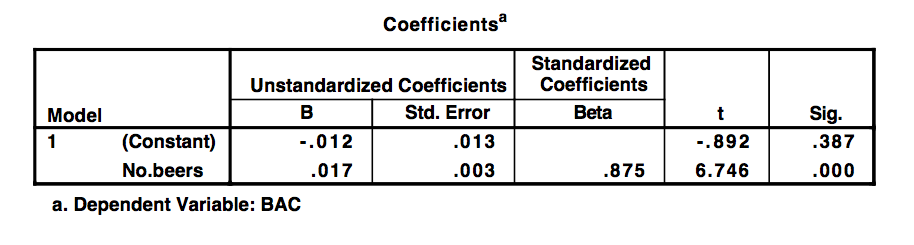
\includegraphics[width=70mm]{chapters/Chapter_14/ext_figure/zRegF.png}
   
   \label{fig:f12_11}
\end{figure}

    \begin{enumerate}
    \item 0.017
    \item 0.17
    \item 1.7
    \item 17
    \item 170
    \end{enumerate}
    
    \framebox[5cm][l]{ Answer: }

  \end{exercise}
  \begin{solution}    % 4
  
     $ BAC = -0.012 + 0.017 (9) = 0.14 $
     
  \end{solution}

  \begin{exercise} % 5            %%%%%%%%%%%%%%%%%%%%

    How well does the \\ number of beers a student drinks predict his or her
blood alcohol content (BAC)? Sociology researchers, at Ohio State University, \\ wanted to know if there is a relationship between the amount of beer consumed and \\ BAC. The researchers assigned the number of cans of \\ beer to each student. After each student had consumed the assigned number of beers,  \\ thirty minutes later, an officer of the law \\ measured the students BAC. \\ \cite{OSU2016}  A scatterplot of the data appears below.  The scatterplot shows

\begin{knitrout}\footnotesize
\definecolor{shadecolor}{rgb}{0.969, 0.969, 0.969}\color{fgcolor}

{\centering \includegraphics[width=7cm]{figure/LBL16f-1} 

}



\end{knitrout}

      \begin{enumerate}
      \item a weak negative relationship.
      \item a moderately high negative correlation.
      \item almost no connection.
      \item a small positive correlation.
      \item a moderately high positive straight-line relationship between some beers and \\ BAC.
      \end{enumerate}
      \vspace{5mm}
      \framebox[5cm][l]{ Answer: }

  \end{exercise}
  \begin{solution}    % 5
  
    A moderately strong positive straight-line relationship between number of beers and BAC.
  
  \end{solution}

  \begin{exercise} % 6         %%%%%%%%%%%%%%%%%%%%%%%%%%%%%%

    How well does the \\ number of beers a student drinks predict his or her
blood alcohol content (BAC)? Sociology researchers, at Ohio State University, \\ wanted to know if there is a relationship between the amount of beer consumed and \\ BAC. The researchers assigned the number of cans of \\ beer to each student. After each student had consumed the assigned number of beers, \\ thirty minutes later, an officer of the law \\ measured the students BAC.  \\ \cite{OSU2016}
A scatterplot of the data appears below.  A plausible value of the correlation between number of beers and blood alcohol content, based on the scatterplot, is

\begin{figure}[htbp] %  figure placement: here, top, bottom, or page
   \centering
   % \caption{Number of Beers vs. BAC}
   \includegraphics[width=60mm]{chapters/Chapter_14/ext_figure/zCorF.png}
   \label{fig:f12_14}
\end{figure}

      \begin{enumerate}
      \item $r = -0.875$.
      \item $r = -0.765$.
      \item $r$ close to 0.
      \item $r = 0.765$.
      \item $r = 0.875$.
      \end{enumerate}

      % \vspace{5mm}

    \framebox[5cm][l]{ Answer: }

    \end{exercise}
    \begin{solution}  % 6
    
      % The correllation coefficient is $r = 0.875 = \sqrt{0.765}$ where  $r^2$ is the coefficient of determination.
       
    \end{solution}


  \begin{exercise} % 7        %%%%%%%%%%%%%%%%%%%%%%%%%%%%%%%%

    STEP 1: In the next six tasks, we will use the data from GSS2014 in this exercise.  We have been asked to examine the relationship between a person's height \\ and a person's income.  Here we have {\textit{income}} which is an  interval-ratio type of variable  \\ while {\textit{height}} is also an interval-ratio type of variable.  These types of variables require \\ that we use a Simple Linear Regression (SLR) \\ analysis.  So step 1 in the process of analysis is to choose the an independent and dependent variables.  Note: In the GSS2014 dataset, {\textit{height}} is  known as HEIGHT and {\textit{income}} is \\ known as rincom06.

\begin{figure}[ht]

{\centering \includegraphics[width=7cm]{figure/LBL16h-1} 

}

\caption[Respondent's Height vs]{Respondent's Height vs. Income}\label{fig:LBL16h}
\end{figure}



{\tiny{
  \begin{verbatim}

Call:
lm(formula = Income ~ Height)

Residuals:
    Min      1Q  Median      3Q     Max 
-16.322  -2.706   1.044   3.865   9.492 

Coefficients:
            Estimate Std. Error t value Pr(>|t|)  
(Intercept)  -7.6415     9.9800  -0.766   0.4457  
Height        0.3467     0.1502   2.308   0.0231 *
---
Signif. codes:  0 '***' 0.001 '**' 0.01 '*' 0.05 '.' 0.1 ' ' 1

Residual standard error: 5.499 on 98 degrees of freedom
Multiple R-squared:  0.05156,	Adjusted R-squared:  0.04189 
F-statistic: 5.328 on 1 and 98 DF,  p-value: 0.02309


  \end{verbatim}
}}

    \vspace{5mm}
    \framebox[5cm][l]{ Answer: }

    \end{exercise}
    \begin{solution}    % 7

       The independent variable is HEIGHT and the dependent variable is rincom06.

    \end{solution}

  \begin{exercise} % 8

    STEP 2: Using the information from exercise four, we must state the hypotheses about its relationship \\ between {\textit{income}} and {\textit{height}}.  Based on our experience, how should we state our hypotheses?

    \vspace{5mm}
    \framebox[5cm][l]{ Answer: }

    \end{exercise}
    \begin{solution}    % 8

       $H_0: \beta = 0" vs. $H_1: \beta \ne 0$

    \end{solution}

  \begin{exercise} % 9

    STEP 3: Using the information from exercise four, determine the coefficient of determination.  Recall that this value is also referred to as r-squared.

    \vspace{5mm}
    \framebox[5cm][l]{ Answer: }

    \end{exercise}
    \begin{solution}    % 9

       The correlation coefficient between the respondent's height and income is 0.0515649

    \end{solution}

  \begin{exercise} % 10

    STEP 4: Using the information from exercise four, record the independent, dependent variables, and the correlation coefficient.

{\scriptsize{
    \begin{table}[ht]
    \centering
    \begin{tabular}{lr} \hline
        &  \multicolumn{1}{c}{Independent} \\ \hline

    Dep. Var. & 1. \underline{\phantom{xxxxxxxx}}      \\ \hline
    1. \underline{\phantom{xxxxxxxx}}  &  \underline{\phantom{xxxxxxxx}}       \\ \hline

    \end{tabular}
    \end{table}
}}

  % \vspace{5mm}
  % \framebox[7cm][l]{ Answer: }

    \end{exercise}
    \begin{solution}    % 10

       \begin{table}[ht]
    \centering
    \begin{tabular}{lr} \hline
        &  \multicolumn{1}{c}{Independent} \\ \hline

    Dep. Var. & 1. height      \\ \hline
    1. income  &   0.2270792      \\ \hline

    \end{tabular}
    \end{table}

    \end{solution}

      \begin{exercise} % 11


    STEP 5: Using the information from exercise four, describe the results of the independent variable.  Identify variables that we tested, their strength and direction of the relationship.  We should distinguish the relationship in general terms \\ and refer the statistical value in parentheses.  Also not whether the hypotheses were supported.

    \vspace{10mm}
    \framebox[5cm][l]{ Answer: }

    \end{exercise}
    \begin{solution}      % 11

    For a sample of 40 subjects, we tested the relationship between height and income.  We found a weak positive relationship using the correlation coefficient (0.2270792).  We then looked at the slope:  as {\textit{height}} increases by one inch, {\textit{income}} increases by 0.346722 with a p-value of

    \end{solution}

  \begin{exercise} % 12

    STEP 1:  In the next six tasks, we will use a sample of 100 subjects from the GSS2014 data in this exercise.  We have been asked to examine the relationship between a person's income, age, and ``not \\ married'' and a person's happiness.  Here we have variables which are  interval-ratio type of variable.  These types of variables require that we use a Simple Linear Regression (SLR) analysis.  So step 1 in the process of analysis is choosing independent and dependent variables.  Note: In the GSS2014 dataset, {\textit{happy}} is known as GENERAL HAPPINESS, {\textit{income06}} is known as TOTAL FAMILY INCOME, {\textit{age}} is known as AGE OF RESPONDENT, and {\textit{absingle}} is known as NOT MARRIED.

{\small{
% latex table generated in R 4.0.2 by xtable 1.8-4 package
% Fri Jul 31 12:47:45 2020
\begin{table}[ht]
\centering
\begin{tabular}{rrrrr}
  \hline
 & 1 & 2 & 3 & 4 \\ 
  \hline
1 & 1.00 & -0.08 & -0.25 & 0.03 \\ 
  2 & -0.08 & 1.00 & -0.07 & -0.16 \\ 
  3 & -0.25 & -0.07 & 1.00 & -0.27 \\ 
  4 & 0.03 & -0.16 & -0.27 & 1.00 \\ 
   \hline
\end{tabular}
\end{table}

}}

{\tiny{
  \begin{verbatim}

Call:
lm(formula = Happiness ~ Age + Income + NotMarried)

Residuals:
    Min      1Q  Median      3Q     Max 
-1.1546 -0.5515  0.1941  0.4034  1.5019 

Coefficients:
             Estimate Std. Error t value Pr(>|t|)    
(Intercept)  2.551920   0.419007   6.090 2.32e-08 ***
Age         -0.004007   0.003817  -1.050  0.29644    
Income      -0.029958   0.011223  -2.669  0.00893 ** 
NotMarried  -0.075195   0.131933  -0.570  0.57004    
---
Signif. codes:  0 '***' 0.001 '**' 0.01 '*' 0.05 '.' 0.1 ' ' 1

Residual standard error: 0.6161 on 96 degrees of freedom
Multiple R-squared:  0.07479,	Adjusted R-squared:  0.04587 
F-statistic: 2.587 on 3 and 96 DF,  p-value: 0.05754


  \end{verbatim}
}}

What are the dependent and independent \\ variables?

    \vspace{5mm}
    \framebox[5cm][l]{ Answer: }

    \end{exercise}
    \vspace{2mm}
    \begin{solution}      % 12

       The independent variable is income,   age, and absingle and the dependent variable is happiness.

    \end{solution}

  \begin{exercise} % 13

    STEP 2: Using the information from exercise nine, we must state the hypotheses about its relationship \\ between  {\textit{Happiness}}, {\textit{income}}, and {\textit{age}}.  Based on our experience, how should we state our hypotheses?

    \vspace{5mm}
    \framebox[7cm][l]{ Answer: }

    \end{exercise}
    \vspace{2mm}
    \begin{solution}      %  13

       $H_0: \beta_1 = \beta_2 = \beta_3 = 0$ \\
       $H_1:$ at least one slope is not equal zero. \\
       where $\beta_1$ is the slope for Happiness and Income,  $\beta_2$ is the slope for Happiness and Age and $\beta_3$ is         the slope for Happiness and single.

    \end{solution}


  \begin{exercise} % 14

    STEP 3: Using the information from exercise 12, determine the \\ coefficient of determination.

    \vspace{5mm}
    \framebox[5cm][l]{ Answer: }

    \end{exercise}
    \begin{solution}      % 14

       Read the results from the computer generated output.

    \end{solution}

  \begin{exercise} % 15

    STEP 4: Using the information from exercise 12, record the independent, dependent variables, and the correlation coefficients.

     \begin{table}[ht]
     \centering
     {\tiny{
     \begin{tabular}{lrrrr} \hline
         &  \multicolumn{3}{c}{Independent} \\ \hline

     Dep. Var. & 1. \underline{\phantom{xxxx}} &
                 2. \underline{\phantom{xxxx}} &
                 3. \underline{\phantom{xxxx}} &
                 4. \underline{\phantom{xxxx}} \\ \hline
     1. \underline{\phantom{xxxx}}  &
     \underline{\phantom{xxxx}}  \\ \hline
     2. \underline{\phantom{xxxx}}  &
     \underline{\phantom{xxxx}} &
     \underline{\phantom{xxxx}}  \\ \hline
     3. \underline{\phantom{xxxx}}  &
     \underline{\phantom{xxxx}} &
     \underline{\phantom{xxxx}} &
     \underline{\phantom{xxxx}}  \\ \hline
     4. \underline{\phantom{xxxx}}  &
     \underline{\phantom{xxxx}} &
     \underline{\phantom{xxxx}} &
     \underline{\phantom{xxxx}} &
     \underline{\phantom{xxxx}}  \\ \hline
     \end{tabular}
     }}
     \end{table}

  %  \vspace{5mm}
  %  \framebox[5cm][l]{ Answer: }

    \end{exercise}
    \begin{solution}    % 15

      The results are in the table.

    \end{solution}

  \begin{exercise} % 16

    STEP 5:  Using the information from exercise 12,  record the independent, dependent  variables, and the correlation coefficients.

    \vspace{5mm}
    \framebox[5cm][l]{ Answer: }

    \end{exercise}
    \begin{solution}    % 16

  The results are in the table.

    \end{solution}

  \begin{exercise} % 17

    STEP 1:  In the next six tasks, we will use all of the data from \\ GSS2014 in this exercise.  We have been \\ asked to examine the relationship between a person's income, age, and ``not married'' and a person's happiness.  Here we have variables which are  interval-ratio type of variable.  \\ These types of variables require that we use a Simple Linear Regression (SLR) analysis.  So step 1 in the process of analysis is choosing independent and dependent variables.  Note: In the GSS2014 dataset, {\textit{happy}} is known as GENERAL HAPPINESS, {\textit{income06}} is known as TOTAL FAMILY INCOME, {\textit{age}} is \\ known as AGE OF RESPONDENT, and \\ {\textit{absingle}} is known as NOT MARRIED.

{\small{
% latex table generated in R 4.0.2 by xtable 1.8-4 package
% Fri Jul 31 12:47:45 2020
\begin{table}[ht]
\centering
\begin{tabular}{rrrrr}
  \hline
 & 1 & 2 & 3 & 4 \\ 
  \hline
1 & 1.00 & 0.02 & -0.00 & -0.01 \\ 
  2 & 0.02 & 1.00 & 0.00 & 0.02 \\ 
  3 & -0.00 & 0.00 & 1.00 & 0.06 \\ 
  4 & -0.01 & 0.02 & 0.06 & 1.00 \\ 
   \hline
\end{tabular}
\end{table}

}}

{\tiny{
  \begin{verbatim}

Call:
lm(formula = Happiness ~ Age + Income + NotMarried)

Residuals:
    Min      1Q  Median      3Q     Max 
-1.2435 -0.6599  0.1324  0.2881  1.3956 

Coefficients:
              Estimate Std. Error t value Pr(>|t|)    
(Intercept)  2.3173217  0.0923286  25.099   <2e-16 ***
Age          0.0001357  0.0009617   0.141    0.888    
Income      -0.0264172  0.0028697  -9.205   <2e-16 ***
NotMarried  -0.0290415  0.0336223  -0.864    0.388    
---
Signif. codes:  0 '***' 0.001 '**' 0.01 '*' 0.05 '.' 0.1 ' ' 1

Residual standard error: 0.6378 on 1516 degrees of freedom
Multiple R-squared:  0.05344,	Adjusted R-squared:  0.05156 
F-statistic: 28.53 on 3 and 1516 DF,  p-value: < 2.2e-16


  \end{verbatim}
}}

What are the dependent and independent \\ variables?

    \vspace{5mm}
    \framebox[7cm][l]{ Answer: }

    \end{exercise}
    \begin{solution}      % 17
       
       The independent variable is income,   age, and absingle and the dependent variable is happiness.
       
    \end{solution}

  \begin{exercise} % 18

    STEP 2: Using the information from exercise 17, we must state the hypotheses about its relationship between \\ {\textit{Happiness}}, {\textit{income}}, and {\textit{age}}.  Based on our experience, how should we state our hypotheses?

    \vspace{5mm}
    \framebox[7cm][l]{ Answer: }

    \end{exercise}
    \vspace{2mm}
    \begin{solution}      % 18

       $H_0: \beta_1 = \beta_2 = \beta_3 = 0$ \\
       $H_1:$ at least one slope is not equal zero. \\
       where $\beta_1$ is the slope for Happiness and Income,  $\beta_2$ is the slope for Happiness and Age and $\beta_3$ is         the slope for Happiness and single.

    \end{solution}

  \begin{exercise} % 19

    STEP 3: Using the information from exercise nine, determine the coefficient of determination.

    \vspace{5mm}
    \framebox[7cm][l]{ Answer: }

    \end{exercise}
    \begin{solution}    % 19

       Read the results from the computer generated output.

    \end{solution}

  \begin{exercise} % 20


    STEP 4: Using the information from exercise 17, record the independent, dependent variables, and the correlation coefficients.

     \begin{table}[ht]
     \centering
     {\tiny{
     \begin{tabular}{lrrrr} \hline
         &  \multicolumn{3}{c}{Independent} \\ \hline

     Dep. Var. & 1. \underline{\phantom{xxxx}} &
                 2. \underline{\phantom{xxxx}} &
                 3. \underline{\phantom{xxxx}} &
                 4. \underline{\phantom{xxxx}} \\ \hline
     1. \underline{\phantom{xxxx}}  &
     \underline{\phantom{xxxx}}  \\ \hline
     2. \underline{\phantom{xxxx}}  &
     \underline{\phantom{xxxx}} &
     \underline{\phantom{xxxx}}  \\ \hline
     3. \underline{\phantom{xxxx}}  &
     \underline{\phantom{xxxx}} &
     \underline{\phantom{xxxx}} &
     \underline{\phantom{xxxx}}  \\ \hline
     4. \underline{\phantom{xxxx}}  &
     \underline{\phantom{xxxx}} &
     \underline{\phantom{xxxx}} &
     \underline{\phantom{xxxx}} &
     \underline{\phantom{xxxx}}  \\ \hline
     \end{tabular}
     }}
     \end{table}

  %  \vspace{5mm}
  %  \framebox[7cm][l]{ Answer: }

    \end{exercise}
    \vspace{2mm}
    \begin{solution}    % 20

      The results are in the table.

    \end{solution}

  \begin{exercise} % 21

    STEP 5:

    Using the information from exercise 17, \\  record the independent, dependent \\ variables, and the correlation coefficients.


  %  \vspace{5mm}
  %  \framebox[7cm][l]{ Answer: }

    \end{exercise}
    \begin{solution}    % 21

  The results are in the table.


    \end{solution}


\end{exercises}

\onecolumn


%!Rnw root = ../../Main.Rnw

\chapter{Workshops}
\label{chap:ch17}

% \section{Workshop 1A}         %%%%%%%%%%%%%%%%%%%%%%%%%%%%%%%%%%

\clearpage
\begin{exercises}
    \begin{exercise}  % 1A        %%%%%%%%%%%%%%%%%%
    
    \begin{center}
\begin{flushleft}\textbf{ \large \hfill Workshop 1A, Submitted by: }\end{flushleft}

\fbox{\parbox{14cm}{
\vspace{4mm}
Name: \underline{\phantom{xxxxxxxxxxxxxxxxxxxxxxxx}} Signature: \underline{\phantom{xxxxxxxxxxxxxxxxxxxxxxxx}}

\vspace{4mm}
Name: \underline{\phantom{xxxxxxxxxxxxxxxxxxxxxxxx}} Signature: \underline{\phantom{xxxxxxxxxxxxxxxxxxxxxxxx}}

\vspace{4mm}
Name: \underline{\phantom{xxxxxxxxxxxxxxxxxxxxxxxx}} Signature: \underline{\phantom{xxxxxxxxxxxxxxxxxxxxxxxx}}

\vspace{4mm}
Name: \underline{\phantom{xxxxxxxxxxxxxxxxxxxxxxxx}} Signature: \underline{\phantom{xxxxxxxxxxxxxxxxxxxxxxxx}}
 }}
 \end{center}

\begin{minipage}[ht]{8.9cm}

{\footnotesize{
Table 17.1: A partial list of students registered for  Stat \\ 1600 during Fall 2016 of their Major course of study.

%\begin{table}[ht]
\centering
%\caption{A partial list of students registered for Stat 1600 during Fall 2016 of their Major course of study.}
\begin{tabular}{@{} l | cccccc | c @{}} \hline
& \multicolumn{5}{c}{Class } \\ \hline
Major & A & B & C & D & Web & Total & RF \\ \hline
Anthropology & 2 &   &   & 1 &   & 3 & \\
Art           &   & 5 & 3 & 1 &   & 9 & \\
Aviation      &   &   & 1 & 1 &   & 2 & \\
Biology       &   & 3 &   & 1 & 1 & 5 & \\
Business      & 1 &   &   &   &   & 1 & \\
Communication & 5 & 1 & 4 & 3 & 4 & 17 & \\
Criminal Justice &  & 3 & 2 & 1 &   & 6 & \\
Data Science  &   & 1 &   &   &   & 1 & \\
Education     &   & 2 &   &   & 2 & 4 & \\
English       & 2 & 3 &   &   & 1 & 6 & \\
Foreign Lang. &   & 1 & 1 &   &   & 2 & \\
Geography     &   & 1 &   &   & 1 & 2 & \\
Graphic Design & 1 &  & 1 &   &   & 2 & \\
History       & 1 &   & 1 &   &   & 2 & \\
Journalism    &   & 1 & 1 &   & 1 & 3 & \\
Mathematics   &   & 2 &   &   &   & 2 & \\
Music         & 2 &   & 7 & 3 & 3 & 15 & \\
Nursing       &   & 1 &   &   &   & 1 & \\
Physics       &   &   &   & 1 &   & 1 & \\
Psychology    &12 & 9 & 9 & 8 & 6 & 44 & \\
Social Work   & 6 & 6 & 6 & 5 & 3 & 26 & \\
Sociology      &   & 1 &   & 1 &   & 2 & \\ \hline
Total         &32 &40 &36 &26 &22 &156 &   \\ \hline
\end{tabular}
%\end{table}
}}

\end{minipage}  \hfill
\begin{minipage}[ht]{5.8cm}
    
    Using the data from Table 17.1,

\begin{enumerate}
  \item Construct a  relative \\ frequency table for total student majors (column above).
  \item	The highest percentage of \\ students fall under \\ what major?
  \item	What percentage of students are Art majors?
  \item	What percentage of \\ students'  majors fall in both Sociology and Psychology?
  \item	How does the percentage \\ of students who are  \\ communications  majors \\ in Class A compare to \\ the  percentage of   communication majors  overall for total students? 
\end{enumerate}

\end{minipage}

    \end{exercise}
    \begin{solution}
      
  \begin{enumerate}
  \item Construct a relative frequency table for total student majors (column above).
  \item	The highest percentage of students fall under what major?
  \item	What percentage of students are Art majors?
  \item	What percentage of  students’ majors fall in both Sociology and Psychology?
  \item	How does the percentage of students who are communications majors in Class A compare to the percentage of communication majors overall for total students? 
\end{enumerate}  

    \end{solution}
  
\clearpage

    \begin{exercise}  % 1B        %%%%%%%%%%%%%%%%%%

    \begin{center}

\begin{flushleft}\textbf{ \large \hfill Workshop 1B, Submitted by: }\end{flushleft}

\fbox{\parbox{14cm}{
\vspace{4mm}
Name: \underline{\phantom{xxxxxxxxxxxxxxxxxxxxxxxx}} Signature: \underline{\phantom{xxxxxxxxxxxxxxxxxxxxxxxx}}

\vspace{4mm}
Name: \underline{\phantom{xxxxxxxxxxxxxxxxxxxxxxxx}} Signature: \underline{\phantom{xxxxxxxxxxxxxxxxxxxxxxxx}}

\vspace{4mm}
Name: \underline{\phantom{xxxxxxxxxxxxxxxxxxxxxxxx}} Signature: \underline{\phantom{xxxxxxxxxxxxxxxxxxxxxxxx}}

\vspace{4mm}
Name: \underline{\phantom{xxxxxxxxxxxxxxxxxxxxxxxx}} Signature: \underline{\phantom{xxxxxxxxxxxxxxxxxxxxxxxx}}
 }}
\end{center}

\begin{minipage}[ht]{8.9cm}

{\footnotesize{
Table 17.2: A partial list of students registered for Stat \\ 1600 during Fall 2016 of their Major course of study.

%\begin{table}[ht]
\centering
% \caption{A partial list of students registered for Stat 1600 during Fall 2016 of their Major course of study.}
\begin{tabular}{@{} l | cccccc | c @{}} \hline
& \multicolumn{5}{c}{Class } \\ \hline
Major & A & B & C & D & Web & Total & RF \\ \hline
Anthropology & 2 &   &   & 1 &   & 3 & \\
Art           &   & 5 & 3 & 1 &   & 9 & \\
Aviation      &   &   & 1 & 1 &   & 2 & \\
Biology       &   & 3 &   & 1 & 1 & 5 & \\
Business      & 1 &   &   &   &   & 1 & \\
Communication & 5 & 1 & 4 & 3 & 4 & 17 & \\
Criminal Justice &  & 3 & 2 & 1 &   & 6 & \\
Data Science  &   & 1 &   &   &   & 1 & \\
Education     &   & 2 &   &   & 2 & 4 & \\
English       & 2 & 3 &   &   & 1 & 6 & \\
Foreign Lang. &   & 1 & 1 &   &   & 2 & \\
Geography     &   & 1 &   &   & 1 & 2 & \\
Graphic Design & 1 &  & 1 &   &   & 2 & \\
History       & 1 &   & 1 &   &   & 2 & \\
Journalism    &   & 1 & 1 &   & 1 & 3 & \\
Mathematics   &   & 2 &   &   &   & 2 & \\
Music         & 2 &   & 7 & 3 & 3 & 15 & \\
Nursing       &   & 1 &   &   &   & 1 & \\
Physics       &   &   &   & 1 &   & 1 & \\
Psychology    &12 & 9 & 9 & 8 & 6 & 44 & \\
Social Work   & 6 & 6 & 6 & 5 & 3 & 26 & \\
Sociology      &   & 1 &   & 1 &   & 2 & \\ \hline
Total         &32 &40 &36 &26 &22 &156 &   \\ \hline
\end{tabular}
%\end{table}
}}

\end{minipage}
\begin{minipage}[ht]{5.8cm}

    Using the data from Table 17.2,

\begin{enumerate}
  \item	Using the column \\ `RF' above, construct a \\ relative frequency table for student majors in the Web Class only.
  \item	The highest percentage \\ of students fall under what major?
  \item	What percentage of students are Music majors?
  \item	What percentage of students are found in the majors of Psychology, Social Work and Sociology (combined)?
  \item	How does the percentage of \\ students who are \\ education  majors in the Web class compare to  the \\ percentage of  education \\ majors overall for total \\ students?  Which is higher?
\end{enumerate}

\end{minipage}
    \end{exercise}
    \begin{solution} % 1B

  \begin{enumerate}
  \item	Using the column `RF' above, construct a relative frequency table for student majors in the Web Class only.
  \item	The highest percentage of students fall under what major?
  \item	What percentage of students are Music majors?
  \item	What percentage of students are found in the majors of Psychology, Social Work and Sociology (combined)?
  \item	How does the percentage of students who are education majors in the Web class compare to the percentage of education majors overall for total students?  Which is higher?
\end{enumerate}
    \end{solution}

\clearpage

    \begin{exercise}  % 1C        %%%%%%%%%%%%%%%%%%

    \begin{center}
\begin{flushleft}\textbf{ \large \hfill Workshop 1C, Submitted by: }\end{flushleft}

\fbox{\parbox{14cm}{
\vspace{4mm}
Name: \underline{\phantom{xxxxxxxxxxxxxxxxxxxxxxxx}} Signature: \underline{\phantom{xxxxxxxxxxxxxxxxxxxxxxxx}}

\vspace{4mm}
Name: \underline{\phantom{xxxxxxxxxxxxxxxxxxxxxxxx}} Signature: \underline{\phantom{xxxxxxxxxxxxxxxxxxxxxxxx}}

\vspace{4mm}
Name: \underline{\phantom{xxxxxxxxxxxxxxxxxxxxxxxx}} Signature: \underline{\phantom{xxxxxxxxxxxxxxxxxxxxxxxx}}

\vspace{4mm}
Name: \underline{\phantom{xxxxxxxxxxxxxxxxxxxxxxxx}} Signature: \underline{\phantom{xxxxxxxxxxxxxxxxxxxxxxxx}}
 }}
\end{center}

Hospital-acquired infections are a serious concern for patients in hospitals and can be caused by bacterial, viral, and fungal pathogens.  Suppose hospitals in the state of Michigan reported the following number of infections and deaths from infection below for the past year.

\begin{table}[ht]
\centering
\caption{Hospital-acquired Infections}
\begin{tabular}{@{} lcc @{}} \hline
%  & \multicolumn{5}{c}{Class } \\ \hline
Type of infection & Number of Infections & Number of Deaths \\ \hline
Pneumonia & 184 & 79 \\
Bloodstream & 258 & 65 \\
Surgical site &	361 & 12 \\
Urinary tract	&	833 & 103 \\
Other	& 287 & 54 \\ \hline
\end{tabular}
\end{table}

    Using the data from Table 17.1,

\begin{enumerate}
  \item What type of variable is `type of infection' numerical or categorical?
  \item	We can further describe this variable as \underline{\phantom{xxxxxxxxxxxxxxx}}.
  \item	Construct a relative frequency table for the number of infections (show percentages to two places past the decimal).
  \item	Complete a bar chart for the relative frequency table above complete with title and axis Labels.
  \item	What other type of graph can we use for this variable type?
\end{enumerate}

    \end{exercise}
    \begin{solution} % 1C

  \begin{enumerate}
  \item	Using the column `RF' above, construct a relative frequency table for student majors in the Web Class only.
  \item	The highest percentage of students fall under what major?
  \item	What percentage of students are Music majors?
  \item	What percentage of students are found in the majors of Psychology, Social Work and Sociology (combined)?
  \item	How does the percentage of students who are education majors in the Web class compare to the percentage of education majors overall for total students?  Which is higher?
\end{enumerate}

    \end{solution}


\clearpage

    \begin{exercise}  % 2A        %%%%%%%%%%%%%%%%%%

    \begin{center}
\begin{flushleft}\textbf{ \large \hfill Workshop 2A, Submitted by: }\end{flushleft}

\fbox{\parbox{14cm}{
\vspace{4mm}
Name: \underline{\phantom{xxxxxxxxxxxxxxxxxxxxxxxx}} Signature: \underline{\phantom{xxxxxxxxxxxxxxxxxxxxxxxx}}

\vspace{4mm}
Name: \underline{\phantom{xxxxxxxxxxxxxxxxxxxxxxxx}} Signature: \underline{\phantom{xxxxxxxxxxxxxxxxxxxxxxxx}}

\vspace{4mm}
Name: \underline{\phantom{xxxxxxxxxxxxxxxxxxxxxxxx}} Signature: \underline{\phantom{xxxxxxxxxxxxxxxxxxxxxxxx}}

\vspace{4mm}
Name: \underline{\phantom{xxxxxxxxxxxxxxxxxxxxxxxx}} Signature: \underline{\phantom{xxxxxxxxxxxxxxxxxxxxxxxx}}
 }}
\end{center}

The average test grades of 19 students are as follows (on a scale from 0 to 100, with 100 being the highest score):

91 (A), 95 (A), 96 (A), 82 (B), 94 (A), 75 (C), 91 (A), 79 (C), 92 (A), 100 (A), 89 (B), 93(A), 91 (A), 86 (B), 93 (A), 72 (C), 74 (C), 93 (A), 90 (A)

\begin{table}[ht]
\centering
\caption{Distribution of Grades}
\begin{tabular}{@{} lcc @{}} \hline
%%  & \multicolumn{5}{c}{Class } \\ \hline
grades & frequency & relative frequency \\ \hline
A  & & \\
B  & & \\
C  & & \\ \hline
\end{tabular}
\end{table}

\begin{enumerate}
  \item Fill in the frequency and relative frequency table above
  \item  Create a bar chart and pie chart for the above data
  \item  What percentage of students got a grade of `A'?
  \item  Looking at the bar chart in part a, identify the shape of the data (symmetric, \\ right-skewed, left-skewed)?
\end{enumerate}

    \end{exercise}
    \begin{solution}  % 2A

  \begin{enumerate}
  \item Fill in the frequency and relative frequency table above
  \item  Create a bar chart and pie chart for the above data
  \item  What percentage of students got a grade of `A'?
  \item  Looking at the bar chart in part a, identify the shape of the data (symmetric, right-skewed, left-skewed)?
\end{enumerate}

    \end{solution}

\clearpage

    \begin{exercise}  % 2B        %%%%%%%%%%%%%%%%%%

    \begin{center}
\begin{flushleft}\textbf{\large \hfill Workshop 2B, Submitted by: }\end{flushleft}

\fbox{\parbox{14cm}{
\vspace{4mm}
Name: \underline{\phantom{xxxxxxxxxxxxxxxxxxxxxxxx}} Signature: \underline{\phantom{xxxxxxxxxxxxxxxxxxxxxxxx}}

\vspace{4mm}
Name: \underline{\phantom{xxxxxxxxxxxxxxxxxxxxxxxx}} Signature: \underline{\phantom{xxxxxxxxxxxxxxxxxxxxxxxx}}

\vspace{4mm}
Name: \underline{\phantom{xxxxxxxxxxxxxxxxxxxxxxxx}} Signature: \underline{\phantom{xxxxxxxxxxxxxxxxxxxxxxxx}}

\vspace{4mm}
Name: \underline{\phantom{xxxxxxxxxxxxxxxxxxxxxxxx}} Signature: \underline{\phantom{xxxxxxxxxxxxxxxxxxxxxxxx}}
 }}
\end{center}

The following 50 test scores for Stat 1600 students are found below. Based on the intervals provided, complete the relative frequency table and answer the following questions.

84	88	76	44	80	83	51	93	69	78 \\
49	55	78	93	64	84	54	92	96	72 \\
97	37	97	67	83	93	95	67	72	67 \\
86	76	80	58	62	69	64	82	48	54 \\
80	69  62	67	66	73	77	82	84	86

\begin{table}[ht]
\centering
\caption{Distribution of Test Scores}
\begin{tabular}{@{} lcc @{}} \hline
%  & \multicolumn{5}{c}{Class } \\ \hline
Grades  & frequency & relative frequency \\ \hline
30-39 & & \\
40-49 & & \\
50-59 & & \\
60-69 & & \\
70-79 & & \\
80-89 & & \\
90-99 & & \\ \hline
\end{tabular}
\end{table}

\begin{enumerate}
  \item Fill in the frequency and relative frequency above.
  \item	Complete a stem and leaf plot with the stem representing the 10’s place and using 3-9.
  \item Draw a histogram for the test scores using the intervals in the relative frequency table above.
  \item	What percentage of students had scores of 59 or less?
\end{enumerate}

    \end{exercise}
    \begin{solution} %2B

  \begin{enumerate}
  \item Fill in the frequency and relative frequency above.
  \item	Complete a stem and leaf plot with the stem representing the 10’s place and using 3-9.
  \item Draw a histogram for the test scores using the intervals in the relative frequency table above.
  \item	What percentage of students had scores of 59 or less?
\end{enumerate}

    \end{solution}

\clearpage

    \begin{exercise}  % 2C        %%%%%%%%%%%%%%%%%%

    \begin{center}
\begin{flushleft}\textbf{\large \hfill Workshop 2C, Submitted by: }\end{flushleft}

\fbox{\parbox{14cm}{
\vspace{4mm}
Name: \underline{\phantom{xxxxxxxxxxxxxxxxxxxxxxxx}} Signature: \underline{\phantom{xxxxxxxxxxxxxxxxxxxxxxxx}}

\vspace{4mm}
Name: \underline{\phantom{xxxxxxxxxxxxxxxxxxxxxxxx}} Signature: \underline{\phantom{xxxxxxxxxxxxxxxxxxxxxxxx}}

\vspace{4mm}
Name: \underline{\phantom{xxxxxxxxxxxxxxxxxxxxxxxx}} Signature: \underline{\phantom{xxxxxxxxxxxxxxxxxxxxxxxx}}

\vspace{4mm}
Name: \underline{\phantom{xxxxxxxxxxxxxxxxxxxxxxxx}} Signature: \underline{\phantom{xxxxxxxxxxxxxxxxxxxxxxxx}}
 }}
\end{center}

The numbers of absences for 20 Stat 1600 students are shown below (on a scale from 0 to 30).

Sample:	10, 0, 1, 3, 15, 6, 2, 1, 0, 21, 25, 11, 9, 7, 4, 5, 12, 28, 17, 8

Sorted:	0, 0, 1, 1, 2, 3, 4, 5, 6, 7, 8, 9, 10, 11, 12, 15, 17, 21, 25, 28


\begin{table}[ht]
\centering
\caption{Distribution of Absences}
\begin{tabular}{@{} lcc @{}} \hline
%  & \multicolumn{5}{c}{Class } \\ \hline
Number of absences & Frequency & Relative frequency \\
0-9 & & \\
10-19 & & \\
20-29 & & \\ \hline
\end{tabular}
\end{table}

\begin{enumerate}
  \item	Fill in the frequency and relative frequency above.
  \item	Complete a stem and leaf plot with the stem representing the 10's place and using 0-2.
  \item	Draw a histogram for the absences using the intervals in the relative frequency table above.
  \item	What percentage of students had number of absences less than 20?
\end{enumerate}

    \end{exercise}
    \begin{solution} % 2C

\begin{enumerate}
  \item	Fill in the frequency and relative frequency above.
  \item	Complete a stem and leaf plot with the stem representing the 10's place and using 0-2.
  \item	Draw a histogram for the absences using the intervals in the relative frequency table above.
  \item	What percentage of students had number of absences less than 20?
\end{enumerate}

    \end{solution}

\clearpage

    \begin{exercise}  % 3A         %%%%%%%%%%%%%%%%%%

    \begin{center}
\begin{flushleft}\textbf{\large \hfill Workshop 3A, Submitted by: }\end{flushleft}

\fbox{\parbox{14cm}{
\vspace{4mm}
Name: \underline{\phantom{xxxxxxxxxxxxxxxxxxxxxxxx}} Signature: \underline{\phantom{xxxxxxxxxxxxxxxxxxxxxxxx}}

\vspace{4mm}
Name: \underline{\phantom{xxxxxxxxxxxxxxxxxxxxxxxx}} Signature: \underline{\phantom{xxxxxxxxxxxxxxxxxxxxxxxx}}

\vspace{4mm}
Name: \underline{\phantom{xxxxxxxxxxxxxxxxxxxxxxxx}} Signature: \underline{\phantom{xxxxxxxxxxxxxxxxxxxxxxxx}}

\vspace{4mm}
Name: \underline{\phantom{xxxxxxxxxxxxxxxxxxxxxxxx}} Signature: \underline{\phantom{xxxxxxxxxxxxxxxxxxxxxxxx}}
 }}
\end{center}

% {\small{
The number of ice cream cones sold during a single day in the middle of August was tracked for surrounding stores.  Consider the following stem and leaf and answer the  questions below. The stem represents `10's' and the leaves represent `1's'.  For instance, the first number represented is 14 (14 ice cream cones were sold at one store).

\vspace{-4mm}

{\small{
\begin{verbatim}

  The decimal point is 1 digit(s) to the right of the |

  1 | 46
  2 | 2358
  3 | 0446779
  4 | 1359
  5 | 46


\end{verbatim}
}}

\vspace{-4mm}

\begin{minipage}[ht]{7cm}

{\small{Give the five-number summary of the data:}}

\vspace{-2mm}

{\small{
\begin{enumerate}
  \item Make sure to show your work!
  \begin{enumerate}
    \item What is the MIN?
    \item	What is Q1?
    \item	What is the MED?
    \item What is Q3?
    \item What is the MAX?
  \end{enumerate}

  \item Draw a boxplot for the data.
  \item Describe the shape of the \\ distribution (symmetric, right skewed, or left skewed).
  \item Ice Cream sales for a single day in January were tracked among several shops.  Would we use a histogram or bar chart to represent this data?  Why?  Draw the correct chart (histogram or bar chart).
\end{enumerate}
}}

\end{minipage} \hfill
\begin{minipage}[bht]{7cm}

{\small{
\begin{tabular}{@{} lc @{}} \hline
Cold Stone Creamery	& 18 \\
Culver's &	16 \\
Ritter's &	9 \\
Treat Street &	3 \\
Y'OPA &	20 \\
Yo Go Delites &	24 \\ \hline
\end{tabular}
}}
\end{minipage}

\end{exercise}
\begin{solution} % 3A

\begin{enumerate}
  \item	Fill in the frequency and relative frequency above.
  \item	Complete a stem and leaf plot with the stem representing the 10's place and using 0-2.
  \item	Draw a histogram for the absences using the intervals in the relative frequency table above.
  \item	What percentage of students had number of absences less than 20?
\end{enumerate}

    \end{solution}

\clearpage

    \begin{exercise}  % 3B         %%%%%%%%%%%%%%%%%

    \begin{center}
\begin{flushleft}\textbf{\large \hfill Workshop 3B, Submitted by: }\end{flushleft}

\fbox{\parbox{14cm}{
\vspace{4mm}
Name: \underline{\phantom{xxxxxxxxxxxxxxxxxxxxxxxx}} Signature: \underline{\phantom{xxxxxxxxxxxxxxxxxxxxxxxx}}

\vspace{4mm}
Name: \underline{\phantom{xxxxxxxxxxxxxxxxxxxxxxxx}} Signature: \underline{\phantom{xxxxxxxxxxxxxxxxxxxxxxxx}}

\vspace{4mm}
Name: \underline{\phantom{xxxxxxxxxxxxxxxxxxxxxxxx}} Signature: \underline{\phantom{xxxxxxxxxxxxxxxxxxxxxxxx}}

\vspace{4mm}
Name: \underline{\phantom{xxxxxxxxxxxxxxxxxxxxxxxx}} Signature: \underline{\phantom{xxxxxxxxxxxxxxxxxxxxxxxx}}
 }}
\end{center}

The age at inauguration for each U.S. President is provided below:

52, 69, 64, 46, 54, 47, 70, 61, 57, 57, 58, 57, 61, 54, 68, 51, 49, 64, 57, 50, 48, 65, 52, 56, 46, 54, 56, 55, 51, 54, 51, 60, 62, 43, 55, 56, 61, 49, 51, 47, 55, 55, 54, 42, 51

https://www.loc.gov/rr/program/bib/inaugurations/


\begin{enumerate}
  \item Give the five-number summary of the data:
  {\small{
    \begin{enumerate}
    \item What is the MIN?
    \item What is Q1?
    \item What is the MED?
    \item What is Q3?
    \item What is the MAX?
    \end{enumerate}
  }}
    \item Draw a boxplot for the data.
    \item Finish the relative frequency table below.

{\small{
\begin{tabular}{@{} lcc @{}} \hline
Age & Frequency & Relative frequency \\ \hline
40 - 44 & & \\
45 - 49 & & \\
50 - 54 & & \\
55 - 59 & & \\
60 - 64 & & \\
65 - 69 & & \\
70 - 74 & & \\
\end{tabular}
}}

    \item	Construct a histogram based on the given intervals for age at inauguration.  Describe the shape of the distribution (symmetric, right skewed, or left skewed).
    \item Do some extra research: Who was the youngest president at inauguration? Who was the oldest president at inauguration?
\end{enumerate}

    \end{exercise}
    \begin{solution} % 3B

\begin{enumerate}
  \item	Fill in the frequency and relative frequency above.
  \item	Complete a stem and leaf plot with the stem representing the 10's place and using 0-2.
  \item	Draw a histogram for the absences using the intervals in the relative frequency table above.
  \item	What percentage of students had number of absences less than 20?
\end{enumerate}

    \end{solution}

\clearpage

    \begin{exercise}  % 3C         %%%%%%%%%%%%%%%%%

    \begin{center}
\begin{flushleft}\textbf{\large \hfill Workshop 3C, Submitted by: }\end{flushleft}

\fbox{\parbox{14cm}{
\vspace{4mm}
Name: \underline{\phantom{xxxxxxxxxxxxxxxxxxxxxxxx}} Signature: \underline{\phantom{xxxxxxxxxxxxxxxxxxxxxxxx}}

\vspace{4mm}
Name: \underline{\phantom{xxxxxxxxxxxxxxxxxxxxxxxx}} Signature: \underline{\phantom{xxxxxxxxxxxxxxxxxxxxxxxx}}

\vspace{4mm}
Name: \underline{\phantom{xxxxxxxxxxxxxxxxxxxxxxxx}} Signature: \underline{\phantom{xxxxxxxxxxxxxxxxxxxxxxxx}}

\vspace{4mm}
Name: \underline{\phantom{xxxxxxxxxxxxxxxxxxxxxxxx}} Signature: \underline{\phantom{xxxxxxxxxxxxxxxxxxxxxxxx}}
 }}
\end{center}

The independence years of some Caribbean and African countries are shown below:

1804, 1847, 1910, 1922, 1941, 1951, 1956, 1956, 1956, 1956, 1956, 1957, 1958, 1958,\\ 1960, 1960,  1960, 1960, 1960,1960, 1960, 1960, 1960, 1961, 1961, 1962, 1962, 1966, \\ 1966, 1973, 1974, 1975, 1977, 1978, 1979, 1979, 1980, 1981, 1981, 1983, 1990, 1993

$n = 42$

\begin{enumerate}
  \item Give the five-number summary of the data:
  {\small{
  \begin{enumerate}
  \item What is the MIN?
  \item What is Q1?
  \item What is the MED?
  \item What is Q3?
  \item What is the MAX?
\end{enumerate}
}}
\item Draw a boxplot for the data.
\item Finish the relative frequency table below.

{\small{
\begin{tabular}{@{} lcc @{}} \hline
Age & Frequency & Relative frequency \\ \hline
1800 – 1839 & & \\
1840 – 1879 & & \\
1880 – 1919	& & \\
1920 – 1959	& & \\
1960 – 1999	& & \\
\end{tabular}
}}
\item	Construct a histogram based on the given intervals for independence year. Describe the shape of the distribution (symmetric, right skewed, or left skewed).
\item Do some extra (but fun) research: Which country has the minimum (first) independence year on this list?
\end{enumerate}
\end{exercise}
\begin{solution}  % 3C

\end{solution}

\clearpage

    \begin{exercise}  % 4A         %%%%%%%%%%%%%%%%%

    \begin{center}
\begin{flushleft}\textbf{\large \hfill Workshop 4A, Submitted by: }\end{flushleft}

\fbox{\parbox{14cm}{
\vspace{4mm}
Name: \underline{\phantom{xxxxxxxxxxxxxxxxxxxxxxxx}} Signature: \underline{\phantom{xxxxxxxxxxxxxxxxxxxxxxxx}}

\vspace{4mm}
Name: \underline{\phantom{xxxxxxxxxxxxxxxxxxxxxxxx}} Signature: \underline{\phantom{xxxxxxxxxxxxxxxxxxxxxxxx}}

\vspace{4mm}
Name: \underline{\phantom{xxxxxxxxxxxxxxxxxxxxxxxx}} Signature: \underline{\phantom{xxxxxxxxxxxxxxxxxxxxxxxx}}

\vspace{4mm}
Name: \underline{\phantom{xxxxxxxxxxxxxxxxxxxxxxxx}} Signature: \underline{\phantom{xxxxxxxxxxxxxxxxxxxxxxxx}}
 }}
\end{center}

A local bank has been monitoring daily average wait-times for its customers for four weeks. The manager believed that she could improve the wait-times by having one(1) permanent clerk and three(3) floating clerks, instead of the current three (3) permanent clerks. The floating clerks would do other tasks except when the lines became excessive. Last week the manager implemented the new system.

Old Policy:   5, 7, 10, 11, 18, 4, 4, 4, 14, 21, 0, 7, 8, 9, 18, 6, 6, 12, 22, 25 \\
New Policy: 4, 3, 9, 13, 17

Were waiting times longer using the ``Old Policy'' or the ``New Policy?''  To answer this question, calculate the following for both the old and new policies.

\begin{enumerate}
  \item Draw comparison dotplots for the samples above.
  \item For each sample, calculate the mean AND median.  Locate (place) these on your dotplots, clearly distinguishing between the two.
  % \item What is the mode for the old policy?
  \item Calculate the 10\% trimmed mean for the old policy.  How does this change from the regular mean?
\end{enumerate}

\end{exercise}
\begin{solution}  % 4a

\end{solution}

\clearpage

    \begin{exercise}  % 4B         %%%%%%%%%%%%%%%%%

    \begin{center}
\begin{flushleft}\textbf{\large \hfill Workshop 4B, Submitted by: }\end{flushleft}

\fbox{\parbox{14cm}{
\vspace{4mm}
Name: \underline{\phantom{xxxxxxxxxxxxxxxxxxxxxxxx}} Signature: \underline{\phantom{xxxxxxxxxxxxxxxxxxxxxxxx}}

\vspace{4mm}
Name: \underline{\phantom{xxxxxxxxxxxxxxxxxxxxxxxx}} Signature: \underline{\phantom{xxxxxxxxxxxxxxxxxxxxxxxx}}

\vspace{4mm}
Name: \underline{\phantom{xxxxxxxxxxxxxxxxxxxxxxxx}} Signature: \underline{\phantom{xxxxxxxxxxxxxxxxxxxxxxxx}}

\vspace{4mm}
Name: \underline{\phantom{xxxxxxxxxxxxxxxxxxxxxxxx}} Signature: \underline{\phantom{xxxxxxxxxxxxxxxxxxxxxxxx}}
 }}
\end{center}

Annual chocolate sales in billions of dollars from 6 countries are provided below.

\$2.5, \$1.9, \$4.2, \$1.2, \$3.3, \$19.1

For the data above calculate:

\begin{enumerate}
  \item Mean
  \item Median
  \item 10 percent trimmed mean   % Median of Pairwise Averages
\end{enumerate}
\end{exercise}
\begin{solution}  % 4b

\end{solution}

\clearpage

    \begin{exercise}  % 4C         %%%%%%%%%%%%%%%%%

    \begin{center}
\begin{flushleft}\textbf{\large \hfill Workshop 4C, Submitted by: }\end{flushleft}

\fbox{\parbox{14cm}{
\vspace{4mm}
Name: \underline{\phantom{xxxxxxxxxxxxxxxxxxxxxxxx}} Signature: \underline{\phantom{xxxxxxxxxxxxxxxxxxxxxxxx}}

\vspace{4mm}
Name: \underline{\phantom{xxxxxxxxxxxxxxxxxxxxxxxx}} Signature: \underline{\phantom{xxxxxxxxxxxxxxxxxxxxxxxx}}

\vspace{4mm}
Name: \underline{\phantom{xxxxxxxxxxxxxxxxxxxxxxxx}} Signature: \underline{\phantom{xxxxxxxxxxxxxxxxxxxxxxxx}}

\vspace{4mm}
Name: \underline{\phantom{xxxxxxxxxxxxxxxxxxxxxxxx}} Signature: \underline{\phantom{xxxxxxxxxxxxxxxxxxxxxxxx}}
 }}
\end{center}

Weekly costs of lattes for 5 WMU graduate students are provided below.

\$3.47, \$12, \$7.52, \$10.5, \$4.5

\begin{enumerate}
  \item Mean
  \item Median
  \item 20 percent trimmed mean   % Median of Pairwise Averages
\end{enumerate}
\end{exercise}
\begin{solution}  % 4c

\end{solution}

\clearpage

    \begin{exercise}  % 5A         %%%%%%%%%%%%%%%%%

    \begin{center}
\begin{flushleft}\textbf{\large \hfill Workshop 5A, Submitted by: }\end{flushleft}

\fbox{\parbox{14cm}{
\vspace{4mm}
Name: \underline{\phantom{xxxxxxxxxxxxxxxxxxxxxxxx}} Signature: \underline{\phantom{xxxxxxxxxxxxxxxxxxxxxxxx}}

\vspace{4mm}
Name: \underline{\phantom{xxxxxxxxxxxxxxxxxxxxxxxx}} Signature: \underline{\phantom{xxxxxxxxxxxxxxxxxxxxxxxx}}

\vspace{4mm}
Name: \underline{\phantom{xxxxxxxxxxxxxxxxxxxxxxxx}} Signature: \underline{\phantom{xxxxxxxxxxxxxxxxxxxxxxxx}}

\vspace{4mm}
Name: \underline{\phantom{xxxxxxxxxxxxxxxxxxxxxxxx}} Signature: \underline{\phantom{xxxxxxxxxxxxxxxxxxxxxxxx}}
 }}
\end{center}

The average MCAT scores for Michigan medical schools are provided below.

504, 507, 507, 516, 508, 514

\begin{enumerate}
  \item Calculate the overall mean
  \item Calculate the SD
  \item How does Michigan's mean and SD compare to the national average of matriculants (those enrolled in medical schools) 508.7 and SD of 6.9?  Which has greater variability?
\end{enumerate}

http://www.mcattestscores.com/usmedicalschoolsmcatscoresGPA.html

https://www.aamc.org/download/321494/data/factstablea16.pdf

\end{exercise}
\begin{solution}  % 5a

\end{solution}

\clearpage

    \begin{exercise}  % 5B         %%%%%%%%%%%%%%%%%

    \begin{center}
\begin{flushleft}\textbf{\large \hfill Workshop 5B, Submitted by: }\end{flushleft}

\fbox{\parbox{14cm}{
\vspace{4mm}
Name: \underline{\phantom{xxxxxxxxxxxxxxxxxxxxxxxx}} Signature: \underline{\phantom{xxxxxxxxxxxxxxxxxxxxxxxx}}

\vspace{4mm}
Name: \underline{\phantom{xxxxxxxxxxxxxxxxxxxxxxxx}} Signature: \underline{\phantom{xxxxxxxxxxxxxxxxxxxxxxxx}}

\vspace{4mm}
Name: \underline{\phantom{xxxxxxxxxxxxxxxxxxxxxxxx}} Signature: \underline{\phantom{xxxxxxxxxxxxxxxxxxxxxxxx}}

\vspace{4mm}
Name: \underline{\phantom{xxxxxxxxxxxxxxxxxxxxxxxx}} Signature: \underline{\phantom{xxxxxxxxxxxxxxxxxxxxxxxx}}
 }}
\end{center}

Hourly wage of personnel within a small company are as follows:

\begin{tabular}{@{} ll @{}} \hline
Staff	&	Salary (dollars) \\ \hline
Owner		& 30 \\
Manager	& 21 \\
Worker	& 12 \\
Worker	& 11 \\
Worker	& 9 \\ \hline
\end{tabular}

\begin{enumerate}
  \item Calculate the average hourly wage of the staff.
  \item Calculate the SD
  \item A similar company has a mean hourly wage of \$17 per hour with a SD of 9.75.  Which has greater variability?  How does that relate to the spread of the data?
\end{enumerate}

\end{exercise}
\begin{solution}  % 5b

\end{solution}

\clearpage

    \begin{exercise}  % 5c         %%%%%%%%%%%%%%%%%

    \begin{center}
\begin{flushleft}\textbf{\large \hfill Workshop 5C, Submitted by: }\end{flushleft}

\fbox{\parbox{14cm}{
\vspace{4mm}
Name: \underline{\phantom{xxxxxxxxxxxxxxxxxxxxxxxx}} Signature: \underline{\phantom{xxxxxxxxxxxxxxxxxxxxxxxx}}

\vspace{4mm}
Name: \underline{\phantom{xxxxxxxxxxxxxxxxxxxxxxxx}} Signature: \underline{\phantom{xxxxxxxxxxxxxxxxxxxxxxxx}}

\vspace{4mm}
Name: \underline{\phantom{xxxxxxxxxxxxxxxxxxxxxxxx}} Signature: \underline{\phantom{xxxxxxxxxxxxxxxxxxxxxxxx}}

\vspace{4mm}
Name: \underline{\phantom{xxxxxxxxxxxxxxxxxxxxxxxx}} Signature: \underline{\phantom{xxxxxxxxxxxxxxxxxxxxxxxx}}
 }}
\end{center}

The data below are the weights of six (6) randomly selected kids in a daycare measured in pounds

 13.6, 16.6, 23.5, 10.2, 5.4, 15.0

\begin{enumerate}
  \item What is the average weight of the six kids in pounds?
  \item Suppose the weights of the six kids are measured in kilograms instead. Calculate the average weight of the kids in kilograms (Hint: 1 pound = 0.453592 kilograms).
  \item What is the standard deviation of the weight of the kids in pounds?
\end{enumerate}


\end{exercise}
\begin{solution}  % 5c

\end{solution}


\clearpage

    \begin{exercise}  % 6a         %%%%%%%%%%%%%%%%%

    \begin{center}
\begin{flushleft}\textbf{\large \hfill Workshop 6A, Submitted by: }\end{flushleft}

\fbox{\parbox{14cm}{
\vspace{4mm}
Name: \underline{\phantom{xxxxxxxxxxxxxxxxxxxxxxxx}} Signature: \underline{\phantom{xxxxxxxxxxxxxxxxxxxxxxxx}}

\vspace{4mm}
Name: \underline{\phantom{xxxxxxxxxxxxxxxxxxxxxxxx}} Signature: \underline{\phantom{xxxxxxxxxxxxxxxxxxxxxxxx}}

\vspace{4mm}
Name: \underline{\phantom{xxxxxxxxxxxxxxxxxxxxxxxx}} Signature: \underline{\phantom{xxxxxxxxxxxxxxxxxxxxxxxx}}

\vspace{4mm}
Name: \underline{\phantom{xxxxxxxxxxxxxxxxxxxxxxxx}} Signature: \underline{\phantom{xxxxxxxxxxxxxxxxxxxxxxxx}}
 }}
\end{center}

The following is an excerpt from a New York Times article by Nicholas Bakalar (Feb. 10, 2009).

\begin{quotation}
Lengthy television viewing in adolescence may raise the risk for depression in young adulthood, according to a new report.

The study, in the February issue of The Archives of General Psychiatry, published by the American Medical Association, found a rising risk of depressive symptoms with increasing hours spent watching television.

Researchers used data from a larger analysis of 4,142 adolescents who were not depressed at the start of the study. After seven years of follow-up, more than 7 percent had symptoms of depression.

But while about 6 percent of those who watched less than three hours a day were depressed, more than 17 percent of those who watched more than nine hours a day had depressive symptoms.
\end{quotation}

\begin{enumerate}
  \item The word `raise' in the title implies cause-and-effect, not just association.  When comparing lengthy viewers with those who watch less, what possible    confounders can you think of?
  \item Using one confounder from your answer(s) in (1), draw a pathway graph depicting the possible relationship between confounder, possible cause and outcome.
\end{enumerate}
\end{exercise}
\begin{solution}  % 6a

\end{solution}

\clearpage

    \begin{exercise}  % 6b         %%%%%%%%%%%%%%%%%

    \begin{center}
\begin{flushleft}\textbf{\large \hfill Workshop 6B, Submitted by: }\end{flushleft}

\fbox{\parbox{14cm}{
\vspace{4mm}
Name: \underline{\phantom{xxxxxxxxxxxxxxxxxxxxxxxx}} Signature: \underline{\phantom{xxxxxxxxxxxxxxxxxxxxxxxx}}

\vspace{4mm}
Name: \underline{\phantom{xxxxxxxxxxxxxxxxxxxxxxxx}} Signature: \underline{\phantom{xxxxxxxxxxxxxxxxxxxxxxxx}}

\vspace{4mm}
Name: \underline{\phantom{xxxxxxxxxxxxxxxxxxxxxxxx}} Signature: \underline{\phantom{xxxxxxxxxxxxxxxxxxxxxxxx}}

\vspace{4mm}
Name: \underline{\phantom{xxxxxxxxxxxxxxxxxxxxxxxx}} Signature: \underline{\phantom{xxxxxxxxxxxxxxxxxxxxxxxx}}
 }}
\end{center}

The following is an excerpt from a Reuters article by Amy Norton (July 2011).

\begin{quotation}

Are kids safer with grandparents driving?

When children are involved in a car accident, they are less likely to be injured if grandma or grandpa are driving rather than mom or dad, a new study suggests.

The study, published in the journal Pediatrics, looked at five years' worth of data on U.S. car crashes involving children younger than 16.

It found that when grandparents were at the wheel, 0.7 percent of children were injured in the crash. That compared with 1 percent when parents were driving.

When the researchers considered other factors -- such as the circumstances and severity of the crash -- kids riding with grandparents were half as likely to be injured, versus those riding with their parents.

\end{quotation}

\begin{enumerate}
  \item The title implies cause-and-effect, not just association.  When comparing injury rates between parents driving and grandparents driving, what possible    confounders can you think of?
  \item Using one confounder from your answer(s) in (1), draw a pathway graph depicting the possible relationship between confounder, possible cause and outcome.
\end{enumerate}
\end{exercise}
\begin{solution}  % 6b

\end{solution}

\clearpage

    \begin{exercise}  % 6c         %%%%%%%%%%%%%%%%%

    \begin{center}
\begin{flushleft}\textbf{\large \hfill Workshop 6C, Submitted by: }\end{flushleft}

\fbox{\parbox{14cm}{
\vspace{4mm}
Name: \underline{\phantom{xxxxxxxxxxxxxxxxxxxxxxxx}} Signature: \underline{\phantom{xxxxxxxxxxxxxxxxxxxxxxxx}}

\vspace{4mm}
Name: \underline{\phantom{xxxxxxxxxxxxxxxxxxxxxxxx}} Signature: \underline{\phantom{xxxxxxxxxxxxxxxxxxxxxxxx}}

\vspace{4mm}
Name: \underline{\phantom{xxxxxxxxxxxxxxxxxxxxxxxx}} Signature: \underline{\phantom{xxxxxxxxxxxxxxxxxxxxxxxx}}

\vspace{4mm}
Name: \underline{\phantom{xxxxxxxxxxxxxxxxxxxxxxxx}} Signature: \underline{\phantom{xxxxxxxxxxxxxxxxxxxxxxxx}}
 }}
\end{center}

Frequency of playing violent video games has at times been linked with and seen as a possible cause for those committing violent acts.  Much debate still looms over whether playing violent video games can lead to a desensitization of violence and a lack of compassion for others.

One article that explores these ideas is titled, The Impact of Degree of Exposure to Violent Video Games, Family Background, and Other Factors on Youth Violence, by the authors Whitney Decamp and Christopher Ferguson.  The authors respond to the concern that violence in video games might contribute to youth violence.  There is still no consensus on whether violent video games may be contributing to violence in youth.  The authors sought to study this issue in an ethnically diverse sample of youth in eighth ($n = 5133$) and eleventh grade ($n = 3886$).  Questionnaire surveys were given to the youth to assess a link.  Independent or predictor variables included the playing of violent video games, and an inclination towards violent video games.  Dependent variables included questions pertaining to hitting with the intention to hurt another and taking part in a fight.

Mixed results were reported.  The authors summarized that violent video game play was not significant in 5 of the models used.  There was, however, a positive correlation between games and violent behavior for the models without controls.   When the authors controlled for the propensity and context, however, this suggested the association to be more spurious (not being what it claims to be).  What other factors may be impacting this outcome?

\begin{enumerate}
  \item What possible confounders can you think of for a study of this nature?
  \item Using one confounder from your answer(s) in (1), draw a pathway graph depicting the possible relationships between confounder, possible cause and outcome.
\end{enumerate}
\end{exercise}
\begin{solution}  % 6c

\end{solution}


\clearpage

    \begin{exercise}  % 7a         %%%%%%%%%%%%%%%%%

    \begin{center}
\begin{flushleft}\textbf{\large \hfill Workshop 7A, Submitted by: }\end{flushleft}

\fbox{\parbox{14cm}{
\vspace{4mm}
Name: \underline{\phantom{xxxxxxxxxxxxxxxxxxxxxxxx}} Signature: \underline{\phantom{xxxxxxxxxxxxxxxxxxxxxxxx}}

\vspace{4mm}
Name: \underline{\phantom{xxxxxxxxxxxxxxxxxxxxxxxx}} Signature: \underline{\phantom{xxxxxxxxxxxxxxxxxxxxxxxx}}

\vspace{4mm}
Name: \underline{\phantom{xxxxxxxxxxxxxxxxxxxxxxxx}} Signature: \underline{\phantom{xxxxxxxxxxxxxxxxxxxxxxxx}}

\vspace{4mm}
Name: \underline{\phantom{xxxxxxxxxxxxxxxxxxxxxxxx}} Signature: \underline{\phantom{xxxxxxxxxxxxxxxxxxxxxxxx}}
 }}
\end{center}

Jet design researchers have come up with two new designs for the wings of a rocket plane. They think both designs are an improvement over the old design but want to know which of their new designs performs better at high altitudes. Specifically, they want to know which new design results in more maneuverability at or above 100,000 feet above sea level. They decide to design a randomized trial to study this.


\begin{enumerate}
  \item The researchers include a control group in their design plan. Describe a possible control group. Why did they add it to the study?
  \item Several pilots and planes are lined up for this study. How could the researchers randomize their experiment to avoid confounders?
  \item One way to measure maneuverability is by surveying pilots about how they thought the jets handled. Could a design that asks pilots this question be blinded? If so, how?
  \item Could the design from (2) be double-blinded? If so, how?
  \item What makes single and double blinding important?
\end{enumerate}
\end{exercise}
\begin{solution}  % 7a

\end{solution}

\clearpage

    \begin{exercise}  % 7b         %%%%%%%%%%%%%%%%%

    \begin{center}
\begin{flushleft}\textbf{\large \hfill Workshop 7B, Submitted by: }\end{flushleft}

\fbox{\parbox{14cm}{
\vspace{4mm}
Name: \underline{\phantom{xxxxxxxxxxxxxxxxxxxxxxxx}} Signature: \underline{\phantom{xxxxxxxxxxxxxxxxxxxxxxxx}}

\vspace{4mm}
Name: \underline{\phantom{xxxxxxxxxxxxxxxxxxxxxxxx}} Signature: \underline{\phantom{xxxxxxxxxxxxxxxxxxxxxxxx}}

\vspace{4mm}
Name: \underline{\phantom{xxxxxxxxxxxxxxxxxxxxxxxx}} Signature: \underline{\phantom{xxxxxxxxxxxxxxxxxxxxxxxx}}

\vspace{4mm}
Name: \underline{\phantom{xxxxxxxxxxxxxxxxxxxxxxxx}} Signature: \underline{\phantom{xxxxxxxxxxxxxxxxxxxxxxxx}}
 }}
\end{center}

Some students at WMU were curious about whether partying influences GPA. To find out, they surveyed 100 of their WMU peers, asking each peer only two questions: 1) How many hours a week do you party? 2) What is your GPA? The students then compiled their data and performed an appropriate statistical analysis. They concluded that partying does influence GPA, i.e., the more you party, the lower your GPA.

\begin{enumerate}
  \item What kind of study design is this?
  \item What are advantages of this study design?
  \item What are disadvantages of this study design?
  \item Did the students overlook anything that might have biased or confounded their results?
  \item Suppose the students wanted to correct for something they overlooked. How could they improve their study design?
\end{enumerate}

\end{exercise}
\begin{solution}  % 7b

\end{solution}

\clearpage

    \begin{exercise}  % 7c         %%%%%%%%%%%%%%%%%

    \begin{center}
\begin{flushleft}\textbf{\large \hfill Workshop 7C, Submitted by: }\end{flushleft}

\fbox{\parbox{14cm}{
\vspace{4mm}
Name: \underline{\phantom{xxxxxxxxxxxxxxxxxxxxxxxx}} Signature: \underline{\phantom{xxxxxxxxxxxxxxxxxxxxxxxx}}

\vspace{4mm}
Name: \underline{\phantom{xxxxxxxxxxxxxxxxxxxxxxxx}} Signature: \underline{\phantom{xxxxxxxxxxxxxxxxxxxxxxxx}}

\vspace{4mm}
Name: \underline{\phantom{xxxxxxxxxxxxxxxxxxxxxxxx}} Signature: \underline{\phantom{xxxxxxxxxxxxxxxxxxxxxxxx}}

\vspace{4mm}
Name: \underline{\phantom{xxxxxxxxxxxxxxxxxxxxxxxx}} Signature: \underline{\phantom{xxxxxxxxxxxxxxxxxxxxxxxx}}
 }}
\end{center}

Yogurt is known to contain `friendly bacteria' known generally as probiotics which can benefit the gastrointestinal system.  Many strains of bacteria can be found in yogurt, with some of the most common being, \textit{Lactobacillus bulgaricus}, \textit{Streptococcus thermophilus}, and \textit{Lactobacillus acidophilus}.  Further research has been done suggesting probiotics boost the immune system and may even help in weight management and reduction of disease such as cancer.  A group of researchers decided to investigate this using a questionnaire assessing yogurt consumption (yes/no) and asking questions pertaining to the health of the individuals.

\begin{enumerate}
  \item First of all, what kind of study design is this?
  \item What are advantages of this type of study design?
  \item What are disadvantages of this study design?
  \item	The researchers then separated the results of the surveys for those who said `yes' they consume yogurt to those who said `no' they do not consume yogurt.  They compared the two groups using these as a treatment and control group.  What is wrong with this assumption?
  \item	Suppose the researchers found that those consuming yogurt had better health and concluded that \textit{Lactobacillus bulgaricus} caused a reduction of weight, improved GI and Immune systems.  What are two major problems in this?
  \item	What may be a bias or lead to confounding in this study?
  \item	How could the researchers improve their study design in order to make a conclusion about the effectiveness of \textit{Lactobacillus bulgaricus} and immune system function?
\end{enumerate}

\end{exercise}
\begin{solution}  % 7c

\end{solution}

\clearpage

    \begin{exercise}  % 8a         %%%%%%%%%%%%%%%%%

    \begin{center}
\begin{flushleft}\textbf{\large \hfill Workshop 8A, Submitted by: }\end{flushleft}

\fbox{\parbox{14cm}{
\vspace{4mm}
Name: \underline{\phantom{xxxxxxxxxxxxxxxxxxxxxxxx}} Signature: \underline{\phantom{xxxxxxxxxxxxxxxxxxxxxxxx}}

\vspace{4mm}
Name: \underline{\phantom{xxxxxxxxxxxxxxxxxxxxxxxx}} Signature: \underline{\phantom{xxxxxxxxxxxxxxxxxxxxxxxx}}

\vspace{4mm}
Name: \underline{\phantom{xxxxxxxxxxxxxxxxxxxxxxxx}} Signature: \underline{\phantom{xxxxxxxxxxxxxxxxxxxxxxxx}}

\vspace{4mm}
Name: \underline{\phantom{xxxxxxxxxxxxxxxxxxxxxxxx}} Signature: \underline{\phantom{xxxxxxxxxxxxxxxxxxxxxxxx}}
 }}
\end{center}

Debt Poet's Society

According to a Sallie Mae survey and credit bureau data, in 2008, college students carried an average of \$3,173 debt on their credit cards (USA TODAY, April 13, 2009). Suppose that current credit card debts for all college students have a normal distribution with a mean of \$3,173 and a standard deviation of \$800.

\begin{enumerate}
  \item Find the probability that credit card debt for a randomly selected college student below \$2,109.
  \item Find the probability that credit card debt for a randomly selected college student is above \$3,605.
  \item Find the probability that credit card debt for a randomly selected college student is between \$2,109 and \$3,605.
\end{enumerate}

\end{exercise}
\begin{solution}  % 8a

\end{solution}

\clearpage

    \begin{exercise}  % 8b         %%%%%%%%%%%%%%%%%

    \begin{center}
\begin{flushleft}\textbf{\large \hfill Workshop 8B, Submitted by: }\end{flushleft}

\fbox{\parbox{14cm}{
\vspace{4mm}
Name: \underline{\phantom{xxxxxxxxxxxxxxxxxxxxxxxx}} Signature: \underline{\phantom{xxxxxxxxxxxxxxxxxxxxxxxx}}

\vspace{4mm}
Name: \underline{\phantom{xxxxxxxxxxxxxxxxxxxxxxxx}} Signature: \underline{\phantom{xxxxxxxxxxxxxxxxxxxxxxxx}}

\vspace{4mm}
Name: \underline{\phantom{xxxxxxxxxxxxxxxxxxxxxxxx}} Signature: \underline{\phantom{xxxxxxxxxxxxxxxxxxxxxxxx}}

\vspace{4mm}
Name: \underline{\phantom{xxxxxxxxxxxxxxxxxxxxxxxx}} Signature: \underline{\phantom{xxxxxxxxxxxxxxxxxxxxxxxx}}
 }}
\end{center}

The Social Network

According to an article published on the Web site www.PCMag.com, Facebook users spend an average of 190 minutes per month checking and updating their Facebook pages (Source: http://www.pcmag.com/article2/0,2817,2342757,00.asp). Suppose that the current distribution of time spent per month checking and updating a member's Facebook page is normally distributed with a mean of 190 minutes and a standard deviation of 53.4 minutes. For a randomly selected Facebook member, determine the probability that the amount of time that he or she spends per month checking and updating his or her Facebook page is…

\begin{enumerate}
  \item More than 180 minutes
  \item Less than 120 minutes
  \item Between 120 and 180 minutes
\end{enumerate}

\end{exercise}
\begin{solution}  % 8b

\end{solution}

\clearpage

    \begin{exercise}  % 8c         %%%%%%%%%%%%%%%%%

    \begin{center}
\begin{flushleft}\textbf{\large \hfill Workshop 8C, Submitted by: }\end{flushleft}

\fbox{\parbox{14cm}{
\vspace{4mm}
Name: \underline{\phantom{xxxxxxxxxxxxxxxxxxxxxxxx}} Signature: \underline{\phantom{xxxxxxxxxxxxxxxxxxxxxxxx}}

\vspace{4mm}
Name: \underline{\phantom{xxxxxxxxxxxxxxxxxxxxxxxx}} Signature: \underline{\phantom{xxxxxxxxxxxxxxxxxxxxxxxx}}

\vspace{4mm}
Name: \underline{\phantom{xxxxxxxxxxxxxxxxxxxxxxxx}} Signature: \underline{\phantom{xxxxxxxxxxxxxxxxxxxxxxxx}}

\vspace{4mm}
Name: \underline{\phantom{xxxxxxxxxxxxxxxxxxxxxxxx}} Signature: \underline{\phantom{xxxxxxxxxxxxxxxxxxxxxxxx}}
 }}
\end{center}

The amount paid out by Ajax Insurance Company in a year is normally distributed with mean 3 billion dollars and standard deviation 0.5 billion dollars. The company’s executives consider it a bad year if they must pay out more than 4.25 billion dollars.

\begin{enumerate}
  \item Determine the probability of a bad year.
  \item What is the probability that the company will have a good year?
  \item What is the probability that the company paid out between 2 billion dollars and 3.5 billion dollars?
\end{enumerate}

\end{exercise}
\begin{solution}  % 8c

\end{solution}

\clearpage

    \begin{exercise}  % 9a         %%%%%%%%%%%%%%%%%

    \begin{center}
\begin{flushleft}\textbf{\large \hfill Workshop 9A, Submitted by: }\end{flushleft}

\fbox{\parbox{14cm}{
\vspace{4mm}
Name: \underline{\phantom{xxxxxxxxxxxxxxxxxxxxxxxx}} Signature: \underline{\phantom{xxxxxxxxxxxxxxxxxxxxxxxx}}

\vspace{4mm}
Name: \underline{\phantom{xxxxxxxxxxxxxxxxxxxxxxxx}} Signature: \underline{\phantom{xxxxxxxxxxxxxxxxxxxxxxxx}}

\vspace{4mm}
Name: \underline{\phantom{xxxxxxxxxxxxxxxxxxxxxxxx}} Signature: \underline{\phantom{xxxxxxxxxxxxxxxxxxxxxxxx}}

\vspace{4mm}
Name: \underline{\phantom{xxxxxxxxxxxxxxxxxxxxxxxx}} Signature: \underline{\phantom{xxxxxxxxxxxxxxxxxxxxxxxx}}
 }}
\end{center}

Debt Poet’s Society

According to a Sallie Mae survey and credit bureau data, in 2008, college students carried an average of \$3,173 debt on their credit cards (USA TODAY, April 13, 2009). Suppose that current credit card debts for all college students have a normal distribution with a mean of \$3,173 and a standard deviation of \$800.

\begin{enumerate}
  \item 10\% of the credit card debt for college students is above what value?
  \item 10\% of the credit card debt for college students is below what value?
  \item The middle 80\% of the credit card debt for college students is between what two values?
  \item How likely would it be for a college students to have credit card debt of \$4,500 or more?
\end{enumerate}

\end{exercise}
\begin{solution}  % 9a

\end{solution}

\clearpage

    \begin{exercise}  % 9b         %%%%%%%%%%%%%%%%%

    \begin{center}
\begin{flushleft}\textbf{\large \hfill Workshop 9B, Submitted by: }\end{flushleft}

\fbox{\parbox{14cm}{
\vspace{4mm}
Name: \underline{\phantom{xxxxxxxxxxxxxxxxxxxxxxxx}} Signature: \underline{\phantom{xxxxxxxxxxxxxxxxxxxxxxxx}}

\vspace{4mm}
Name: \underline{\phantom{xxxxxxxxxxxxxxxxxxxxxxxx}} Signature: \underline{\phantom{xxxxxxxxxxxxxxxxxxxxxxxx}}

\vspace{4mm}
Name: \underline{\phantom{xxxxxxxxxxxxxxxxxxxxxxxx}} Signature: \underline{\phantom{xxxxxxxxxxxxxxxxxxxxxxxx}}

\vspace{4mm}
Name: \underline{\phantom{xxxxxxxxxxxxxxxxxxxxxxxx}} Signature: \underline{\phantom{xxxxxxxxxxxxxxxxxxxxxxxx}}
 }}
\end{center}

Tommy Wait, a minor-league baseball pitcher, is notorious for taking an excessive \\ amount of time between pitches. In fact, his times between pitches are normally distributed with a mean of 36 seconds and a standard deviation of 2.5 seconds.

\begin{enumerate}
  \item 10\% of the time between pitches is above what value?
  \item 10\% of the time between pitches is below what value?
  \item The middle 80\% of the time between pitches is between what two values?
  \item How likely would it be for the time between pitches of 40 seconds or more? \end{enumerate}

\end{exercise}
\begin{solution}  % 9b

\end{solution}

\clearpage

    \begin{exercise}  % 9c         %%%%%%%%%%%%%%%%%

    \begin{center}
\begin{flushleft}\textbf{\large \hfill Workshop 9C, Submitted by: }\end{flushleft}

\fbox{\parbox{14cm}{
\vspace{4mm}
Name: \underline{\phantom{xxxxxxxxxxxxxxxxxxxxxxxx}} Signature: \underline{\phantom{xxxxxxxxxxxxxxxxxxxxxxxx}}

\vspace{4mm}
Name: \underline{\phantom{xxxxxxxxxxxxxxxxxxxxxxxx}} Signature: \underline{\phantom{xxxxxxxxxxxxxxxxxxxxxxxx}}

\vspace{4mm}
Name: \underline{\phantom{xxxxxxxxxxxxxxxxxxxxxxxx}} Signature: \underline{\phantom{xxxxxxxxxxxxxxxxxxxxxxxx}}

\vspace{4mm}
Name: \underline{\phantom{xxxxxxxxxxxxxxxxxxxxxxxx}} Signature: \underline{\phantom{xxxxxxxxxxxxxxxxxxxxxxxx}}
 }}
\end{center}

The amount paid out by Ajax Insurance Company in a year is normally distributed with mean 3 billion dollars and standard deviation 0.5 billion dollars. The company’s executives consider it a bad year if they must pay out more than 4.25 billion dollars.

\begin{enumerate}
  \item 18\% of the amount paid out by Ajax Insurance Company is below what amount?
  \item There is a 5\% chance that the company will have to pay more than an amount $x$ (in billions of dollars). What is the value of $x$?
  \item The middle 60\% of the amount paid out by the company is between what two values (in billions of dollars)?
\end{enumerate}

\end{exercise}
\begin{solution}  % 9c

\end{solution}

\clearpage

    \begin{exercise}  % 10a         %%%%%%%%%%%%%%%%%

    \begin{center}
\begin{flushleft}\textbf{\large \hfill Workshop 10A, Submitted by: }\end{flushleft}

\fbox{\parbox{14cm}{
\vspace{4mm}
Name: \underline{\phantom{xxxxxxxxxxxxxxxxxxxxxxxx}} Signature: \underline{\phantom{xxxxxxxxxxxxxxxxxxxxxxxx}}

\vspace{4mm}
Name: \underline{\phantom{xxxxxxxxxxxxxxxxxxxxxxxx}} Signature: \underline{\phantom{xxxxxxxxxxxxxxxxxxxxxxxx}}

Name: \underline{\phantom{xxxxxxxxxxxxxxxxxxxxxxxx}} Signature: \underline{\phantom{xxxxxxxxxxxxxxxxxxxxxxxx}}

\vspace{4mm}
Name: \underline{\phantom{xxxxxxxxxxxxxxxxxxxxxxxx}} Signature: \underline{\phantom{xxxxxxxxxxxxxxxxxxxxxxxx}}
 }}
\end{center}

Drugstore Cowboy

According to an October 27, 2006 article in Newsweek, 60\% of Americans said that they take expired medicines. Suppose that this result is true of the current population of Americans.

\begin{enumerate}
\item Let $x$ be a binomial random variable that denotes the number of American in a random sample of 4 who have taken expired medicines. What are the possible values that $x$ can assume?
\item Find the probability that exactly 2 Americans in a sample of 4 have taken expired medicines.
\item Find the probability that at least 3 Americans in a sample of 4 have taken expired medicines.
\item Find the probability that at most 1 American in a sample of 4 have taken expired medicines.
\end{enumerate}

\end{exercise}
\begin{solution}

\end{solution}


\clearpage

     \begin{exercise}  % 10b         %%%%%%%%%%%%%%%%%

    \begin{center}
\begin{flushleft}\textbf{\large \hfill Workshop 10B, Submitted by: }\end{flushleft}

\fbox{\parbox{14cm}{
\vspace{4mm}
Name: \underline{\phantom{xxxxxxxxxxxxxxxxxxxxxxxx}} Signature: \underline{\phantom{xxxxxxxxxxxxxxxxxxxxxxxx}}

\vspace{4mm}
Name: \underline{\phantom{xxxxxxxxxxxxxxxxxxxxxxxx}} Signature: \underline{\phantom{xxxxxxxxxxxxxxxxxxxxxxxx}}

\vspace{4mm}
Name: \underline{\phantom{xxxxxxxxxxxxxxxxxxxxxxxx}} Signature: \underline{\phantom{xxxxxxxxxxxxxxxxxxxxxxxx}}

\vspace{4mm}
Name: \underline{\phantom{xxxxxxxxxxxxxxxxxxxxxxxx}} Signature: \underline{\phantom{xxxxxxxxxxxxxxxxxxxxxxxx}}
 }}
\end{center}

The Social Network

According to a Harris Interactive poll, 50\% of American college graduates have Facebook accounts. Suppose that this result is true for the current population of American college graduates.

\begin{verbatim}
http://www.harrisinteractive.com/harris_poll/pubs/Harris_Poll_2009_04_16.pdf
\end{verbatim}

\begin{enumerate}
  \item Let $x$ be a binomial random variable that denotes the number of American college graduates in a random sample of 5 who have Facebook accounts. What are the possible values that $x$ can assume?
  \item Find the probability that exactly 3 American college graduates in a sample of 5 have Facebook accounts.
  \item Find the probability that at least 3. American college graduates in a sample of 5 have Facebook accounts.
  \item Find the probability that at most 1 American college graduate in a sample of 5 have Facebook accounts.
\end{enumerate}

\end{exercise}
\begin{solution}  % 10b

\end{solution}


\clearpage

   \begin{exercise}  % 10c        %%%%%%%%%%%%%%%%%

    \begin{center}
\begin{flushleft}\textbf{\large \hfill Workshop 10C, Submitted by: }\end{flushleft}

\fbox{\parbox{14cm}{
\vspace{4mm}
Name: \underline{\phantom{xxxxxxxxxxxxxxxxxxxxxxxx}} Signature: \underline{\phantom{xxxxxxxxxxxxxxxxxxxxxxxx}}

\vspace{4mm}
Name: \underline{\phantom{xxxxxxxxxxxxxxxxxxxxxxxx}} Signature: \underline{\phantom{xxxxxxxxxxxxxxxxxxxxxxxx}}

\vspace{4mm}
Name: \underline{\phantom{xxxxxxxxxxxxxxxxxxxxxxxx}} Signature: \underline{\phantom{xxxxxxxxxxxxxxxxxxxxxxxx}}

\vspace{4mm}
Name: \underline{\phantom{xxxxxxxxxxxxxxxxxxxxxxxx}} Signature: \underline{\phantom{xxxxxxxxxxxxxxxxxxxxxxxx}}
 }}
\end{center}

The Bureau of Labor Statistics reports that in May 2016 that 10.5\% of people who work in the Kalamazoo metropolitan area are employed in production occupations (i.e., making things). Suppose that a random sample of 5 Kalamazoo workers is taken. Let $X$ be a random variable which denotes the number of workers in the sample who are employed in production occupations.

\begin{enumerate}
\item What are the possible values which X can take?
\item Find the probability that exactly 2 of the 5 workers in the sample will be employed in production occupations.
\item Find the probability that at least 3 of the 5 workers in the sample will be employed in production occupations.
\item Find the probability that at most 1 of the 5 workers in the sample will be employed in production occupations.
\end{enumerate}

\end{exercise}
\begin{solution}  % 10c

\end{solution}

\clearpage

    \begin{exercise}  % 11a        %%%%%%%%%%%%%%%%%

    \begin{center}
\begin{flushleft}\textbf{\large \hfill Workshop 11A, Submitted by: }\end{flushleft}

\fbox{\parbox{14cm}{
\vspace{4mm}
Name: \underline{\phantom{xxxxxxxxxxxxxxxxxxxxxxxx}} Signature: \underline{\phantom{xxxxxxxxxxxxxxxxxxxxxxxx}}

\vspace{4mm}
Name: \underline{\phantom{xxxxxxxxxxxxxxxxxxxxxxxx}} Signature: \underline{\phantom{xxxxxxxxxxxxxxxxxxxxxxxx}}

\vspace{4mm}
Name: \underline{\phantom{xxxxxxxxxxxxxxxxxxxxxxxx}} Signature: \underline{\phantom{xxxxxxxxxxxxxxxxxxxxxxxx}}

\vspace{4mm}
Name: \underline{\phantom{xxxxxxxxxxxxxxxxxxxxxxxx}} Signature: \underline{\phantom{xxxxxxxxxxxxxxxxxxxxxxxx}}
 }}
\end{center}

Credit where Credit is Due

According to a May 27, 2009 Minneapolis Star-Tribune article, 78\% of U.S. households have at least one credit card.

Source: http://www.startribune.com/politics/45797562.html

\begin{enumerate}
  \item For a random sample of 500 U.S. households, what is the expected value and standard deviation of the number of U.S. households with at least one credit card.
  \item Using the normal approximation, find the probability that in a random sample of 500 U.S. households, more than 375 households have at least one credit card.
  \item Using the normal approximation, find the probability that in a random sample of 500 U.S. households, less than 385 households have at least one credit card.
  \item Using the normal approximation, find the probability that in a random sample of 500 U.S. households, 376 to 384 households have at least one credit card.
\end{enumerate}

\end{exercise}
\begin{solution}  % 11a

\end{solution}

\clearpage

    \begin{exercise}  % 11b        %%%%%%%%%%%%%%%%%

    \begin{center}
\begin{flushleft}\textbf{\large \hfill Workshop 11B, Submitted by: }\end{flushleft}

\fbox{\parbox{14cm}{
\vspace{4mm}
Name: \underline{\phantom{xxxxxxxxxxxxxxxxxxxxxxxx}} Signature: \underline{\phantom{xxxxxxxxxxxxxxxxxxxxxxxx}}

\vspace{4mm}
Name: \underline{\phantom{xxxxxxxxxxxxxxxxxxxxxxxx}} Signature: \underline{\phantom{xxxxxxxxxxxxxxxxxxxxxxxx}}

\vspace{4mm}
Name: \underline{\phantom{xxxxxxxxxxxxxxxxxxxxxxxx}} Signature: \underline{\phantom{xxxxxxxxxxxxxxxxxxxxxxxx}}

\vspace{4mm}
Name: \underline{\phantom{xxxxxxxxxxxxxxxxxxxxxxxx}} Signature: \underline{\phantom{xxxxxxxxxxxxxxxxxxxxxxxx}}
 }}
\end{center}

Tongue Twister

A 2007 article states that 4.8\% of U.S. households are ``linguistically isolated,'' which means that all members of the household aged 14 years and older have difficulty speaking English.  Assume that this percentage is true for the current population of U.S. households.


 (Source: http://www.antara.co.id/en/arc/2007/9/12/ \newline five-percent-of-us-families-dont-speak-english-report/)


\begin{enumerate}
  \item For a random sample of 750 U.S. households, what is the expected value and standard deviation of the number of U.S. households classified as ``linguistically isolated.''
  \item Using the normal approximation, find the probability that in a random sample of 750 U.S. households, more than 45 would be classified as ``linguistically isolated.''
  \item Using the normal approximation, find the probability that in a random sample of 750 U.S. households, less than 45 would be classified as ``linguistically isolated.''
  \item Using the normal approximation, find the probability that in a random sample of 750 U.S. households, exactly 45 would be classified as ``linguistically isolated.''
\end{enumerate}
\end{exercise}
\begin{solution}  % 11b

\end{solution}

\clearpage

    \begin{exercise}  % 11c        %%%%%%%%%%%%%%%%%

    \begin{center}
\begin{flushleft}\textbf{\large \hfill Workshop 11C, Submitted by: }\end{flushleft}

\fbox{\parbox{14cm}{
\vspace{4mm}
Name: \underline{\phantom{xxxxxxxxxxxxxxxxxxxxxxxx}} Signature: \underline{\phantom{xxxxxxxxxxxxxxxxxxxxxxxx}}

\vspace{4mm}
Name: \underline{\phantom{xxxxxxxxxxxxxxxxxxxxxxxx}} Signature: \underline{\phantom{xxxxxxxxxxxxxxxxxxxxxxxx}}

\vspace{4mm}
Name: \underline{\phantom{xxxxxxxxxxxxxxxxxxxxxxxx}} Signature: \underline{\phantom{xxxxxxxxxxxxxxxxxxxxxxxx}}

\vspace{4mm}
Name: \underline{\phantom{xxxxxxxxxxxxxxxxxxxxxxxx}} Signature: \underline{\phantom{xxxxxxxxxxxxxxxxxxxxxxxx}}
 }}
\end{center}

The Bureau of Labor Statistics reports that in May 2016 that 10.5\% of people who work in the Kalamazoo metropolitan area are employed in production occupations (i.e., making things).

\begin{enumerate}
\item For a random sample of 200 Kalamazoo workers, what is the expected number who will work in production occupations? What is the standard deviation of this?
\item Using the normal approximation, find the probability that in a random sample of 200 Kalamazoo workers, more than 25 will work in production occupations.
\item Using the normal approximation, find the probability that in a random sample of 200 Kalamazoo workers, fewer than 15 will work in production occupations.
\item Using the normal approximation, find the probability that in a random sample of 200 Kalamazoo workers, between 15 and 25 (inclusive) will work in production occupations.
\end{enumerate}

\end{exercise}
\begin{solution}      % 11C


\end{solution}








\end{exercises}

% \clearpage
% 
%     \begin{exercise}  % 12a         %%%%%%%%%%%%%%%%%
% 
%     \begin{center}
% \begin{flushleft}\textbf{\large \hfill Workshop 12A, Submitted by: }\end{flushleft}
% 
% \fbox{\parbox{14cm}{
% \vspace{4mm}
% Name: \underline{\phantom{xxxxxxxxxxxxxxxxxxxxxxxx}} Signature: \underline{\phantom{xxxxxxxxxxxxxxxxxxxxxxxx}}
% 
% \vspace{4mm}
% Name: \underline{\phantom{xxxxxxxxxxxxxxxxxxxxxxxx}} Signature: \underline{\phantom{xxxxxxxxxxxxxxxxxxxxxxxx}}
% 
% \vspace{4mm}
% Name: \underline{\phantom{xxxxxxxxxxxxxxxxxxxxxxxx}} Signature: \underline{\phantom{xxxxxxxxxxxxxxxxxxxxxxxx}}
% 
% \vspace{4mm}
% Name: \underline{\phantom{xxxxxxxxxxxxxxxxxxxxxxxx}} Signature: \underline{\phantom{xxxxxxxxxxxxxxxxxxxxxxxx}}
%  }}
% \end{center}
% 
% Live and Let Dye
% 
% In an experimental study, 44 rats were exposed to a high dose of red dye, 44 rats were exposed to a low dose of red dye, and it was then observed how many in each group developed cancer. 
% 				
% \begin{tabular}{@{} lccc @{}} \hline				
%    & \multicolumn{2}{c}{Cancer} \\ 
% Dose Level of Red Dye &	Yes	 & No &	Total \\ \hline
% High &	14	& 30 &	44 \\ 
% Low &	4 &	40 &	44  \\ \hline
% Total &	18 &	70 & 88 \\ \hline
% \end{tabular}
% 				
% \begin{enumerate}
%   \item Estimate the difference in percentage of developing cancer between high dose level of red dye and low dose level of red dye.
%   \item Calculate a standard error for your estimate in (1).
%   \item Calculate a 95\% confidence interval for the difference in percentage of developing cancer between high dose level of red dye and low dose level of red dye.
% \end{enumerate}
% 
% \end{exercise} 
% \begin{solution}  % 12a
% 
% \end{solution}
% 
% \clearpage
% 
%     \begin{exercise}  % 12b         %%%%%%%%%%%%%%%%%
% 
%     \begin{center}
% \begin{flushleft}\textbf{\large \hfill Workshop 12B, Submitted by: }\end{flushleft}
% 
% \fbox{\parbox{14cm}{
% \vspace{4mm}
% Name: \underline{\phantom{xxxxxxxxxxxxxxxxxxxxxxxx}} Signature: \underline{\phantom{xxxxxxxxxxxxxxxxxxxxxxxx}}
% 
% \vspace{4mm}
% Name: \underline{\phantom{xxxxxxxxxxxxxxxxxxxxxxxx}} Signature: \underline{\phantom{xxxxxxxxxxxxxxxxxxxxxxxx}}
% 
% \vspace{4mm}
% Name: \underline{\phantom{xxxxxxxxxxxxxxxxxxxxxxxx}} Signature: \underline{\phantom{xxxxxxxxxxxxxxxxxxxxxxxx}}
% 
% \vspace{4mm}
% Name: \underline{\phantom{xxxxxxxxxxxxxxxxxxxxxxxx}} Signature: \underline{\phantom{xxxxxxxxxxxxxxxxxxxxxxxx}}
%  }}
% \end{center}
% 
% Gone Fishin'
% 
% Consider the following data from the Chicago Western Electric Study (Shekelle et al., 1981). In the following table 466 men were classified based on death from coronary heart disease (CHD) and fish consumption.
% 				
% \begin{tabular}{@{} lccc @{}} \hline
% & \multicolumn{2}{c}{Death from CHD} \\ 	 		 
% Daily Fish Consumption &	Yes &	No &	Total \\ \hline
% High &	34 &	227 &	261 \\
% Low	& 42 &	163 &	205 \\ \hline
% Total &	76 &	390 &	466 \\ \hline
% \end{tabular}
% 			
% \begin{enumerate}
%   \item Estimate the difference in percentage of death from CHD between high daily fish consumption and low daily fish consumption.
%   \item Calculate a standard error for your estimate in (1).
%   \item Calculate a 95\% confidence interval for the difference in percentage of death from CHD between high daily fish consumption and low daily fish consumption.
% \end{enumerate}
% 			
% 			
% \end{exercise} 
% \begin{solution}  % 12b
% 
% \end{solution}
% 
% \clearpage
% 
%     \begin{exercise}  % 12c         %%%%%%%%%%%%%%%%%
% 
%     \begin{center}
% \begin{flushleft}\textbf{\large \hfill Workshop 12C, Submitted by: }\end{flushleft}
% 
% \fbox{\parbox{14cm}{
% \vspace{4mm}
% Name: \underline{\phantom{xxxxxxxxxxxxxxxxxxxxxxxx}} Signature: \underline{\phantom{xxxxxxxxxxxxxxxxxxxxxxxx}}
% 
% \vspace{4mm}
% Name: \underline{\phantom{xxxxxxxxxxxxxxxxxxxxxxxx}} Signature: \underline{\phantom{xxxxxxxxxxxxxxxxxxxxxxxx}}
% 
% \vspace{4mm}
% Name: \underline{\phantom{xxxxxxxxxxxxxxxxxxxxxxxx}} Signature: \underline{\phantom{xxxxxxxxxxxxxxxxxxxxxxxx}}
% 
% \vspace{4mm}
% Name: \underline{\phantom{xxxxxxxxxxxxxxxxxxxxxxxx}} Signature: \underline{\phantom{xxxxxxxxxxxxxxxxxxxxxxxx}}
%  }}
% \end{center}
% 
% Making the Cut
% 
% The following table shows how many prospective students of a sample of 200 students were admitted to WMU last year, and if the student's GPA was below 2.8 or not.  Out of the sample, 60 applicants were rejected and 140 were accepted. 
% 				
% \begin{tabular}{@{} lccc @{}} \hline				
%  	& \multicolumn{2}{c}{Rejected from WMU} \\   		 
% GPA Below 2.8 &	Yes &	No & Total \\ \hline
% Yes	& 45 &	20 &	65 \\
% No &	15 &	120 &	135 \\ \hline
% Total &	60 &	140 &	200 \\ \hline
% \end{tabular}\begin{enumerate}
%   \item Estimate the difference in proportion of being rejected from WMU between having below a 2.8 GPA and not having below a 2.8 GPA.
%   \item Calculate a standard error for your estimate in (a).  
%   \item Calculate a 95\% confidence interval for the difference in proportion of being rejected from WMU between having below a 2.8 GPA and not having below a 2.8 GPA.
% \end{enumerate}
% 
% \end{exercise} 
% \begin{solution}  % 12c
% 
% \end{solution}
% 
% \clearpage
% 
%     \begin{exercise}  % 13a         %%%%%%%%%%%%%%%%%
% 
%     \begin{center}
% \begin{flushleft}\textbf{\large \hfill Workshop 13A, Submitted by: }\end{flushleft}
% 
% \fbox{\parbox{14cm}{
% \vspace{4mm}
% Name: \underline{\phantom{xxxxxxxxxxxxxxxxxxxxxxxx}} Signature: \underline{\phantom{xxxxxxxxxxxxxxxxxxxxxxxx}}
% 
% \vspace{4mm}
% Name: \underline{\phantom{xxxxxxxxxxxxxxxxxxxxxxxx}} Signature: \underline{\phantom{xxxxxxxxxxxxxxxxxxxxxxxx}}
% 
% \vspace{4mm}
% Name: \underline{\phantom{xxxxxxxxxxxxxxxxxxxxxxxx}} Signature: \underline{\phantom{xxxxxxxxxxxxxxxxxxxxxxxx}}
% 
% \vspace{4mm}
% Name: \underline{\phantom{xxxxxxxxxxxxxxxxxxxxxxxx}} Signature: \underline{\phantom{xxxxxxxxxxxxxxxxxxxxxxxx}}
%  }}
% \end{center}
% 
% Live and Let Dye
% 
% In an experimental study, 44 rats were exposed to a high dose of red dye, 44 rats were exposed to a low dose of red dye, and it was then observed how many in each group developed cancer. 
% 				
% \begin{tabular}{@{} lccc @{}} \hline				
%  	& \multicolumn{2}{c}{Cancer} \\ 			
% Dose Level of Red Dye &	Yes &	No &	Total \\ \hline
% High &	14 &	30 &	44 \\
% Low &	4 &	40 & 44 \\ \hline
% Total &	18 &	70 &	88 \\ \hline
% \end{tabular}
% 				
% \begin{enumerate}
%   \item Estimate the risk ratio of developing cancer between high dose level of red dye and low dose level of red dye.
%   \item Calculate a 95\% confidence interval for the risk ratio of developing cancer between high dose level of red dye and low dose level of red dye.
% \end{enumerate}
% 
% \end{exercise} 
% \begin{solution}  % 13a
% 
% \end{solution}
% 
% \clearpage
% 
%     \begin{exercise}  % 13b         %%%%%%%%%%%%%%%%%
% 
%     \begin{center}
% \begin{flushleft}\textbf{\large \hfill Workshop 13B, Submitted by: }\end{flushleft}
% 
% \fbox{\parbox{14cm}{
% \vspace{4mm}
% Name: \underline{\phantom{xxxxxxxxxxxxxxxxxxxxxxxx}} Signature: \underline{\phantom{xxxxxxxxxxxxxxxxxxxxxxxx}}
% 
% \vspace{4mm}
% Name: \underline{\phantom{xxxxxxxxxxxxxxxxxxxxxxxx}} Signature: \underline{\phantom{xxxxxxxxxxxxxxxxxxxxxxxx}}
% 
% \vspace{4mm}
% Name: \underline{\phantom{xxxxxxxxxxxxxxxxxxxxxxxx}} Signature: \underline{\phantom{xxxxxxxxxxxxxxxxxxxxxxxx}}
% 
% \vspace{4mm}
% Name: \underline{\phantom{xxxxxxxxxxxxxxxxxxxxxxxx}} Signature: \underline{\phantom{xxxxxxxxxxxxxxxxxxxxxxxx}}
%  }}
% \end{center}
% 
% Gone Fishin'
% 
% Consider the following data from the Chicago Western Electric Study (Shekelle et al., 1981). In the following table 466 men were classified based on death from coronary heart disease (CHD) and fish consumption.
% 				
% \begin{tabular}{@{} lccc @{}} \hline				
%  	& \multicolumn{2}{c}{Death from CHD} \\ 				
% Daily Fish Consumption &	Yes &	No &	Total \\ \hline
% High &	34 &	227 &	261 \\
% Low &	42 &	163 &	205 \\ \hline
% Total &	76 &	390 &	466 \\ \hline
% \end{tabular}
% 				
% \begin{enumerate}
%   \item Estimate the risk ratio of death from CHD between high daily fish consumption and low daily fish consumption.
%   \item Calculate a 95\% confidence interval for the risk ratio of death from CHD between high daily fish consumption and low daily fish consumption.
% \end{enumerate}
% 
% \end{exercise} 
% \begin{solution}  % 13b
% 
% \end{solution}
% 
% \clearpage
% 
%     \begin{exercise}  % 13c         %%%%%%%%%%%%%%%%%
% 
%     \begin{center}
% \begin{flushleft}\textbf{\large \hfill Workshop 13C, Submitted by: }\end{flushleft}
% 
% \fbox{\parbox{14cm}{
% \vspace{4mm}
% Name: \underline{\phantom{xxxxxxxxxxxxxxxxxxxxxxxx}} Signature: \underline{\phantom{xxxxxxxxxxxxxxxxxxxxxxxx}}
% 
% \vspace{4mm}
% Name: \underline{\phantom{xxxxxxxxxxxxxxxxxxxxxxxx}} Signature: \underline{\phantom{xxxxxxxxxxxxxxxxxxxxxxxx}}
% 
% \vspace{4mm}
% Name: \underline{\phantom{xxxxxxxxxxxxxxxxxxxxxxxx}} Signature: \underline{\phantom{xxxxxxxxxxxxxxxxxxxxxxxx}}
% 
% \vspace{4mm}
% Name: \underline{\phantom{xxxxxxxxxxxxxxxxxxxxxxxx}} Signature: \underline{\phantom{xxxxxxxxxxxxxxxxxxxxxxxx}}
%  }}
% \end{center}
% 
% Making the Cut
% 
% The following table shows how many prospective students of a sample of 200 students were admitted to WMU last year, and if the student's GPA was below 2.8 or not. Out of the sample, 60 applicants were rejected and 140 were accepted. 
% 			
% \begin{tabular}{@{} lccc @{}} \hline				
%  	& \multicolumn{2}{c}{Rejected from WMU} \\ 		
% GPA Below 2.8 &	Yes &	No &	Total  \\ \hline
% Yes &	45 &	20 &	65 \\
% No &	15 &	120 &	135 \\ \hline
% Total &	60 &	140 &	200 \\ \hline
% \end{tabular}
% 				
% \begin{enumerate}
%   \item Estimate the risk ratio of being rejected from WMU between having below a 2.8 GPA and not having below a 2.8 GPA.
%   \item Calculate a 95\% confidence interval for the risk ratio of being rejected from WMU between having below a 2.8 GPA and not having below a 2.8 GPA.
% \end{enumerate}
% 
% \end{exercise} 
% \begin{solution}  % 13c
% 
% \end{solution}
% 
% \clearpage
% 
%     \begin{exercise}  % 14A         %%%%%%%%%%%%%%%%%
% 
%     \begin{center}
% \begin{flushleft}\textbf{\large \hfill Workshop 14A, Submitted by: }\end{flushleft}
% 
% \fbox{\parbox{14cm}{
% \vspace{4mm}
% Name: \underline{\phantom{xxxxxxxxxxxxxxxxxxxxxxxx}} Signature: \underline{\phantom{xxxxxxxxxxxxxxxxxxxxxxxx}}
% 
% \vspace{4mm}
% Name: \underline{\phantom{xxxxxxxxxxxxxxxxxxxxxxxx}} Signature: \underline{\phantom{xxxxxxxxxxxxxxxxxxxxxxxx}}
% 
% \vspace{4mm}
% Name: \underline{\phantom{xxxxxxxxxxxxxxxxxxxxxxxx}} Signature: \underline{\phantom{xxxxxxxxxxxxxxxxxxxxxxxx}}
% 
% \vspace{4mm}
% Name: \underline{\phantom{xxxxxxxxxxxxxxxxxxxxxxxx}} Signature: \underline{\phantom{xxxxxxxxxxxxxxxxxxxxxxxx}}
%  }}
% \end{center}
% 
% Live and Let Dye
% 
% In an experimental study, 44 rats were exposed to high dose of red dye and 44 rats were exposed to low dose of red dye and then it was observed how many in each group developed cancer.
% 
% \begin{tabular}{@{} lccc @{}} \hline
%  	& \multicolumn{2}{c}{Cancer} \\
% Dose Level of Red Dye &	Yes &	No &	Total \\ \hline
% High &	14 &	30 &	44 \\
% Low	& 4	& 40 &	44 \\ \hline
% Total &	18 &	70 &	88 \\ \hline
% \end{tabular}
% 
% \begin{enumerate}
%   \item Estimate the odds ratio of developing cancer between high dose level of red dye and low dose level of red dye.
%   \item Calculate a 95\% confidence interval for the odds ratio of developing cancer between high dose level of red dye and low dose level of red dye.
% \end{enumerate}
% 
% \end{exercise}
% \begin{solution}  % 14a
% 
% \end{solution}
% 
% \clearpage
% 
%     \begin{exercise}  % 14B         %%%%%%%%%%%%%%%%%
% 
%     \begin{center}
% \begin{flushleft}\textbf{\large \hfill Workshop 14B, Submitted by: }\end{flushleft}
% 
% \fbox{\parbox{14cm}{
% \vspace{4mm}
% Name: \underline{\phantom{xxxxxxxxxxxxxxxxxxxxxxxx}} Signature: \underline{\phantom{xxxxxxxxxxxxxxxxxxxxxxxx}}
% 
% \vspace{4mm}
% Name: \underline{\phantom{xxxxxxxxxxxxxxxxxxxxxxxx}} Signature: \underline{\phantom{xxxxxxxxxxxxxxxxxxxxxxxx}}
% 
% \vspace{4mm}
% Name: \underline{\phantom{xxxxxxxxxxxxxxxxxxxxxxxx}} Signature: \underline{\phantom{xxxxxxxxxxxxxxxxxxxxxxxx}}
% 
% \vspace{4mm}
% Name: \underline{\phantom{xxxxxxxxxxxxxxxxxxxxxxxx}} Signature: \underline{\phantom{xxxxxxxxxxxxxxxxxxxxxxxx}}
%  }}
% \end{center}
% 
% Gone Fishin'
% 
% Consider the following data from the Chicago Western Electric Study (Shekelle et al., 1981). In the following table 466 men were classified based on death from coronary heart disease (CHD) and fish consumption.
% 
% \begin{tabular}{@{} lccc @{}} \hline
%  	& \multicolumn{2}{c}{Death from CHD} \\
% Daily Fish Consumption &	Yes &	No & Total \\ \hline
% Low &	42 &	163 &	205 \\
% High &	34 &	227 &	261 \\ \hline
% Total &	76 &	390 &	466 \\ \hline
% \end{tabular}
% 
% \begin{enumerate}
%   \item Estimate the odds ratio of death from CHD between low daily fish consumption and high daily fish consumption.
%   \item Calculate a 95\% confidence interval for the odds ratio of death from CHD between low daily fish consumption and high daily fish consumption.
% \end{enumerate}
% 
% \end{exercise}
% \begin{solution}  % 14b
% 
% \end{solution}
% 
% \clearpage
% 
%     \begin{exercise}  % 14C         %%%%%%%%%%%%%%%%%
%     
%     \begin{center}
% \begin{flushleft}\textbf{\large \hfill Workshop 14C, Submitted by: }\end{flushleft}
% 
% \fbox{\parbox{14cm}{
% \vspace{4mm}
% Name: \underline{\phantom{xxxxxxxxxxxxxxxxxxxxxxxx}} Signature: \underline{\phantom{xxxxxxxxxxxxxxxxxxxxxxxx}}
% 
% \vspace{4mm}
% Name: \underline{\phantom{xxxxxxxxxxxxxxxxxxxxxxxx}} Signature: \underline{\phantom{xxxxxxxxxxxxxxxxxxxxxxxx}}
% 
% \vspace{4mm}
% Name: \underline{\phantom{xxxxxxxxxxxxxxxxxxxxxxxx}} Signature: \underline{\phantom{xxxxxxxxxxxxxxxxxxxxxxxx}}
% 
% \vspace{4mm}
% Name: \underline{\phantom{xxxxxxxxxxxxxxxxxxxxxxxx}} Signature: \underline{\phantom{xxxxxxxxxxxxxxxxxxxxxxxx}}
%  }}
% \end{center}
% 
% Making the Cut
% 
% The following table shows how many prospective students of a sample of 200 students were admitted to WMU last year, and if the student's GPA was below 2.8 or not. Out of the sample, 60 applicants were rejected and 140 were accepted.
% 
% \begin{tabular}{@{} lccc @{}} \hline
%  	& \multicolumn{2}{c}{Rejected from WMU} \\
% GPA Below 2.8 & 	Yes &	No &	Total \\ \hline
% Yes &	45 &	20 &	65 \\
% No &	15 &	120 &	135 \\ \hline
% Total &	60 &	140 &	200 \\ \hline
% \end{tabular}
% 
% \begin{enumerate}
%   \item Estimate the odds ratio of being rejected from WMU between having below a 2.8 GPA and not having below a 2.8 GPA.
%   \item Calculate a 95\% confidence interval for the odds ratio of being rejected from WMU between having below a 2.8 GPA and not having below a 2.8 GPA.
% \end{enumerate}
% \end{exercise}
% \begin{solution}  % 14c
% 
% \end{solution}
% 
% \clearpage
% 
%     \begin{exercise}  % 15a         %%%%%%%%%%%%%%%%%
%     
%     \begin{center}
% \begin{flushleft}\textbf{\large \hfill Workshop 15A, Submitted by: }\end{flushleft}
% 
% \fbox{\parbox{14cm}{
% \vspace{4mm}
% Name: \underline{\phantom{xxxxxxxxxxxxxxxxxxxxxxxx}} Signature: \underline{\phantom{xxxxxxxxxxxxxxxxxxxxxxxx}}
% 
% \vspace{4mm}
% Name: \underline{\phantom{xxxxxxxxxxxxxxxxxxxxxxxx}} Signature: \underline{\phantom{xxxxxxxxxxxxxxxxxxxxxxxx}}
% 
% \vspace{4mm}
% Name: \underline{\phantom{xxxxxxxxxxxxxxxxxxxxxxxx}} Signature: \underline{\phantom{xxxxxxxxxxxxxxxxxxxxxxxx}}
% 
% \vspace{4mm}
% Name: \underline{\phantom{xxxxxxxxxxxxxxxxxxxxxxxx}} Signature: \underline{\phantom{xxxxxxxxxxxxxxxxxxxxxxxx}}
%  }}
% \end{center}
% 
% The following is an excerpt from a New York Times article by Nicholas Bakalar (Feb. 10, 2009).          
% 
% Lengthy television viewing in adolescence may raise the risk for depression in young adulthood, according to a new report.
% <<<<<<< HEAD
% =======
% 
% The study, in the February issue of The Archives of General Psychiatry, published by the American Medical Association, found a rising risk of depressive symptoms with increasing hours spent watching television.
% 
% Researchers used data from a larger analysis of 4,142 adolescents who were not depressed at the start of the study. After seven years of follow-up, more than 7 percent had symptoms of depression.
% 
% But while about 6 percent of those who watched less than three hours a day were depressed, more than 17 percent of those who watched more than nine hours a day had depressive symptoms.
% 
% \begin{enumerate}
%   \item The word `raise' in the title implies cause-and-effect, not just association.  When comparing lengthy viewers with those who watch less, what possible    confounders can you think of?
%   \item Using one confounder from your answer(s) in (1), draw a pathway graph depicting the possible relationship between confounder, possible cause and outcome.
% \end{enumerate}
% \end{exercise}
% \begin{solution}  % 15a
% 
% \end{solution}
% 
% \clearpage
% 
%     \begin{exercise}  % 15b         %%%%%%%%%%%%%%%%%
%     
%     \begin{center}
% \begin{flushleft}\textbf{\large \hfill Workshop 15B, Submitted by: }\end{flushleft}
% 
% \fbox{\parbox{14cm}{
% \vspace{4mm}
% Name: \underline{\phantom{xxxxxxxxxxxxxxxxxxxxxxxx}} Signature: \underline{\phantom{xxxxxxxxxxxxxxxxxxxxxxxx}}
% 
% \vspace{4mm}
% Name: \underline{\phantom{xxxxxxxxxxxxxxxxxxxxxxxx}} Signature: \underline{\phantom{xxxxxxxxxxxxxxxxxxxxxxxx}}
% 
% \vspace{4mm}
% Name: \underline{\phantom{xxxxxxxxxxxxxxxxxxxxxxxx}} Signature: \underline{\phantom{xxxxxxxxxxxxxxxxxxxxxxxx}}
% 
% \vspace{4mm}
% Name: \underline{\phantom{xxxxxxxxxxxxxxxxxxxxxxxx}} Signature: \underline{\phantom{xxxxxxxxxxxxxxxxxxxxxxxx}}
%  }}
% \end{center}
% 
% The following is an excerpt from a Reuters article by Amy Norton (July 2011).          
% \begin{quote}
% 
% Are kids safer with grandparents driving?
% 
% When children are involved in a car accident, they are less likely to be injured if grandma or grandpa are driving rather than mom or dad, a new study suggests.
% 
% The study, published in the journal Pediatrics, looked at five years' worth of data on U.S. car crashes involving children younger than 16.
% 
% It found that when grandparents were at the wheel, 0.7 percent of children were injured in the crash. That compared with 1 percent when parents were driving.
% 
% When the researchers considered other factors -- such as the circumstances and severity of the crash -- kids riding with grandparents were half as likely to be injured, versus those riding with their parents.
% 
% \end{quote}
% 
% \begin{enumerate}
%   \item The title implies cause-and-effect, not just association.  When comparing injury rates between parents driving and grandparents driving, what possible    confounders can you think of?
%   \item Using one confounder from your answer(s) in (1), draw a pathway graph depicting the possible relationship between confounder, possible cause and outcome.
% \end{enumerate}
% \end{exercise}
% \begin{solution}  % 15b
% 
% \end{solution}
% 
% \clearpage
% 
%     \begin{exercise}  % 15c         %%%%%%%%%%%%%%%%%
%     
%     \begin{center}
% \begin{flushleft}\textbf{\large \hfill Workshop 15C, Submitted by: }\end{flushleft}
% 
% \fbox{\parbox{14cm}{
% \vspace{4mm}
% Name: \underline{\phantom{xxxxxxxxxxxxxxxxxxxxxxxx}} Signature: \underline{\phantom{xxxxxxxxxxxxxxxxxxxxxxxx}}
% 
% \vspace{4mm}
% Name: \underline{\phantom{xxxxxxxxxxxxxxxxxxxxxxxx}} Signature: \underline{\phantom{xxxxxxxxxxxxxxxxxxxxxxxx}}
% 
% \vspace{4mm}
% Name: \underline{\phantom{xxxxxxxxxxxxxxxxxxxxxxxx}} Signature: \underline{\phantom{xxxxxxxxxxxxxxxxxxxxxxxx}}
% 
% \vspace{4mm}
% Name: \underline{\phantom{xxxxxxxxxxxxxxxxxxxxxxxx}} Signature: \underline{\phantom{xxxxxxxxxxxxxxxxxxxxxxxx}}
%  }}
% \end{center}
% 
% Frequency of playing violent video games has at times been linked with and seen as a possible cause for those committing violent acts.  Much debate still looms over whether playing violent video games can lead to a desensitization of violence and a lack of compassion for others.  
% One article that explores these ideas is titled, The Impact of Degree of Exposure to Violent Video Games, Family Background, and Other Factors on Youth Violence, by the authors Whitney Decamp and Christopher Ferguson.  The authors respond to the concern that violence in video games might contribute to youth violence.  There is still no consensus on whether violent video games may be contributing to violence in youth.  The authors sought to study this issue in an ethnically diverse sample of youth in eighth (n=5133) and eleventh grade (n=3886).  Questionnaire surveys were given to the youth to assess a link.  Independent or predictor variables included the playing of violent video games, and an inclination towards violent video games.  Dependent variables included questions pertaining to hitting with the intention to hurt another and taking part in a fight. 
% Mixed results were reported.  The authors summarized that violent video game play was not significant in 5 of the models used.  There was, however, a positive correlation between games and violent behavior for the models without controls.   When the authors controlled for the propensity and context, however, this suggested the association to be more spurious (not being what it claims to be).  What other factors may be impacting this outcome?  
% 
% \begin{enumerate}
%   \item What possible confounders can you think of for a study of this nature?
%   \item Using one confounder from your answer(s) in (1), draw a pathway graph depicting the possible relationships between confounder, possible cause and outcome.
% \end{enumerate}
% \end{exercise}
% \begin{solution}  % 15c
% 
% \end{solution}
% 
% \clearpage
% 
%     \begin{exercise}  % 16a         %%%%%%%%%%%%%%%%%
%     
%     \begin{center}
% \begin{flushleft}\textbf{\large \hfill Workshop 16A, Submitted by: }\end{flushleft}
% 
% \fbox{\parbox{14cm}{
% \vspace{4mm}
% Name: \underline{\phantom{xxxxxxxxxxxxxxxxxxxxxxxx}} Signature: \underline{\phantom{xxxxxxxxxxxxxxxxxxxxxxxx}}
% 
% \vspace{4mm}
% Name: \underline{\phantom{xxxxxxxxxxxxxxxxxxxxxxxx}} Signature: \underline{\phantom{xxxxxxxxxxxxxxxxxxxxxxxx}}
% 
% \vspace{4mm}
% Name: \underline{\phantom{xxxxxxxxxxxxxxxxxxxxxxxx}} Signature: \underline{\phantom{xxxxxxxxxxxxxxxxxxxxxxxx}}
% 
% \vspace{4mm}
% Name: \underline{\phantom{xxxxxxxxxxxxxxxxxxxxxxxx}} Signature: \underline{\phantom{xxxxxxxxxxxxxxxxxxxxxxxx}}
%  }}
% \end{center}
% 
% Jet design researchers have come up with two new designs for the wings of a rocket plane. They think both designs are an improvement over the old design, but want to know which of their new designs performs better at high altitudes. Specifically, they want to know which new design results in more maneuverability at or above 100,000 feet above sea level. They decide to design a randomized trial to study this.
% 
% 
% \begin{enumerate}
%   \item The researchers include a control group in their design plan. Describe a possible control group. Why did they add it to the study?
%   \item Several pilots and planes are lined up for this study. How could the researchers randomize their experiment to avoid confounders?
%   \item One way to measure maneuverability is by surveying pilots about how they thought the jets handled. Could a design that asks pilots this question be blinded? If so, how?
%   \item Could the design from (2) be double-blinded? If so, how?
%   \item What makes single and double blinding important?
% \end{enumerate}
% \end{exercise}
% \begin{solution}  % 16a
% 
% \end{solution}
% 
% \clearpage
% 
%     \begin{exercise}  % 16b         %%%%%%%%%%%%%%%%%
%     
%     \begin{center}
% \begin{flushleft}\textbf{\large \hfill Workshop 16B, Submitted by: }\end{flushleft}
% 
% \fbox{\parbox{14cm}{
% \vspace{4mm}
% Name: \underline{\phantom{xxxxxxxxxxxxxxxxxxxxxxxx}} Signature: \underline{\phantom{xxxxxxxxxxxxxxxxxxxxxxxx}}
% 
% \vspace{4mm}
% Name: \underline{\phantom{xxxxxxxxxxxxxxxxxxxxxxxx}} Signature: \underline{\phantom{xxxxxxxxxxxxxxxxxxxxxxxx}}
% 
% \vspace{4mm}
% Name: \underline{\phantom{xxxxxxxxxxxxxxxxxxxxxxxx}} Signature: \underline{\phantom{xxxxxxxxxxxxxxxxxxxxxxxx}}
% 
% \vspace{4mm}
% Name: \underline{\phantom{xxxxxxxxxxxxxxxxxxxxxxxx}} Signature: \underline{\phantom{xxxxxxxxxxxxxxxxxxxxxxxx}}
%  }}
% \end{center}
% 
% Some students at WMU were curious about whether partying influences GPA. To find out, they surveyed 100 of their WMU peers, asking each peer only two questions: 1) How many hours a week do you party? 2) What is your GPA? The students then compiled their data and performed an appropriate statistical analysis. They concluded that partying does influence GPA, i.e., the more you party, the lower your GPA.
% 
% \begin{enumerate}
%   \item What kind of study design is this?
%   \item What are advantages of this study design?
%   \item What are disadvantages of this study design?
%   \item Did the students overlook anything that might have biased or confounded their results?
%   \item Suppose the students wanted to correct for something they overlooked. How could they improve their study design?
% \end{enumerate}
% 
% \end{exercise}
% \begin{solution}  % 16b
% 
% \end{solution}
% 
% \clearpage
% 
%     \begin{exercise}  % 16c         %%%%%%%%%%%%%%%%%
%     
%     \begin{center}
% \begin{flushleft}\textbf{\large \hfill Workshop 16C, Submitted by: }\end{flushleft}
% 
% \fbox{\parbox{14cm}{
% \vspace{4mm}
% Name: \underline{\phantom{xxxxxxxxxxxxxxxxxxxxxxxx}} Signature: \underline{\phantom{xxxxxxxxxxxxxxxxxxxxxxxx}}
% 
% \vspace{4mm}
% Name: \underline{\phantom{xxxxxxxxxxxxxxxxxxxxxxxx}} Signature: \underline{\phantom{xxxxxxxxxxxxxxxxxxxxxxxx}}
% 
% \vspace{4mm}
% Name: \underline{\phantom{xxxxxxxxxxxxxxxxxxxxxxxx}} Signature: \underline{\phantom{xxxxxxxxxxxxxxxxxxxxxxxx}}
% 
% \vspace{4mm}
% Name: \underline{\phantom{xxxxxxxxxxxxxxxxxxxxxxxx}} Signature: \underline{\phantom{xxxxxxxxxxxxxxxxxxxxxxxx}}
%  }}
% \end{center}
% 
% Yogurt is known to contain `friendly bacteria' known generally as probiotics which can benefit the gastrointestinal system.  Many strains of bacteria can be found in yogurt, with some of the most common being, \textit{Lactobacillus bulgaricus}, \textit{Streptococcus thermophilus}, and \textit{Lactobacillus acidophilus}.  Further research has been done suggesting probiotics boost the immune system and may even help in weight management and reduction of disease such as cancer.  A group of researchers decided to investigate this using a questionnaire assessing yogurt consumption (yes/no) and asking questions pertaining to the health of the individuals.  
% 
% \begin{enumerate}
%   \item First of all, what kind of study design is this?
%   \item What are advantages of this type of study design?
%   \item What are disadvantages of this study design?
%   \item	The researchers then separated the results of the surveys for those who said `yes' they consume yogurt to those who said `no' they do not consume yogurt.  They compared the two groups using these as a treatment and control group.  What is wrong with this assumption?
%   \item	Suppose the researchers found that those consuming yogurt had better health and concluded that \textit{Lactobacillus bulgaricus} caused a reduction of weight, improved GI and Immune systems.  What are two major problems in this?
%   \item	What may be a bias or lead to confounding in this study?
%   \item	How could the researchers improve their study design in order to make a conclusion about the effectiveness of \textit{Lactobacillus bulgaricus} and immune system function?
% \end{enumerate}
% 
% \end{exercise}
% \begin{solution}  % 16c
% 
% \end{solution}
% 
% \clearpage
% 
%     \begin{exercise}  % 17A         %%%%%%%%%%%%%%%%%
%     
%     \begin{center}
% \begin{flushleft}\textbf{\large \hfill Workshop 17A, Submitted by: }\end{flushleft}
% 
% \fbox{\parbox{14cm}{
% \vspace{4mm}
% Name: \underline{\phantom{xxxxxxxxxxxxxxxxxxxxxxxx}} Signature: \underline{\phantom{xxxxxxxxxxxxxxxxxxxxxxxx}}
% 
% \vspace{4mm}
% Name: \underline{\phantom{xxxxxxxxxxxxxxxxxxxxxxxx}} Signature: \underline{\phantom{xxxxxxxxxxxxxxxxxxxxxxxx}}
% 
% \vspace{4mm}
% Name: \underline{\phantom{xxxxxxxxxxxxxxxxxxxxxxxx}} Signature: \underline{\phantom{xxxxxxxxxxxxxxxxxxxxxxxx}}
% 
% \vspace{4mm}
% Name: \underline{\phantom{xxxxxxxxxxxxxxxxxxxxxxxx}} Signature: \underline{\phantom{xxxxxxxxxxxxxxxxxxxxxxxx}}
%  }}
% \end{center}
% 
% Historically throughout the United States, families of four spend about \$239 a week on groceries and food with a standard deviation of 50. Assume a random sample of 250 households is taken in the United States.
% 
% \begin{enumerate}
%   \item What is the expected value of the sample mean.
%   \item	What is the Standard error of this estimate?
%   \item	What is the probability that the mean weekly household spending is more than \$242?
%   \item	What is the probability that the mean weekly household spending less than \$235?
%   \item	What is the probability that the mean weekly household spending is between \$235 and \$242? 
%   \item	If an even larger sample of 2500 households was taken and the SD remains the same, what is the new Standard Error of the estimate? Why did this occur?
% \end{enumerate}
% 
% \end{exercise}
% \begin{solution}  % 17a
% 
% \end{solution}
% 
% \clearpage
% 
%     \begin{exercise}  % 17B         %%%%%%%%%%%%%%%%%
%     
%     \begin{center}
% \begin{flushleft}\textbf{\large \hfill Workshop 17B, Submitted by: }\end{flushleft}
% 
% \fbox{\parbox{14cm}{
% \vspace{4mm}
% Name: \underline{\phantom{xxxxxxxxxxxxxxxxxxxxxxxx}} Signature: \underline{\phantom{xxxxxxxxxxxxxxxxxxxxxxxx}}
% 
% \vspace{4mm}
% Name: \underline{\phantom{xxxxxxxxxxxxxxxxxxxxxxxx}} Signature: \underline{\phantom{xxxxxxxxxxxxxxxxxxxxxxxx}}
% 
% \vspace{4mm}
% Name: \underline{\phantom{xxxxxxxxxxxxxxxxxxxxxxxx}} Signature: \underline{\phantom{xxxxxxxxxxxxxxxxxxxxxxxx}}
% 
% \vspace{4mm}
% Name: \underline{\phantom{xxxxxxxxxxxxxxxxxxxxxxxx}} Signature: \underline{\phantom{xxxxxxxxxxxxxxxxxxxxxxxx}}
%  }}
% \end{center}
% 
% \begin{minipage}[ht]{7cm}
% 
% Too Fast, Not Enough Furious
% 
% The above chart shows the average cost of annual auto insurance premiums in 2008 for drivers with no accidents, one accident, two accidents, and so on. According to this chart, the average annual auto insurance premium for drivers with no accidents was \$1,387 in 2008.
% 
% \end{minipage}
% \begin{minipage}[ht]{7cm}
% 
% %\begin{figure}[ht]
% \centering
%   \includegraphics[width=4cm]{chapters/Workshops/ext_figure/UsaToday.png}
% %\end{figure}
% \end{minipage}
% 
% \begin{enumerate}
%   \item What is the estimated mean annual auto insurance premium for drivers with no accidents?
%   \item	What is the standard error of the estimate assuming this is based on a random sample of 400 drivers? Assume that the standard deviation of auto insurance premiums for all current drivers with no accidents is \$180.
%   \item Assuming the estimate in part a. is the mean for all drivers with no accidents, what is the probability that the mean annual auto insurance premium for drivers with no accidents is greater than \$1,395?
%   \item If a larger random sample of 1600 such drivers was taken and the SD remains the same, what is the new standard error of the estimate?
%   \item Assuming the estimate in part a. is the mean for all drivers with no accidents, what is the probability that the mean annual auto insurance premium for drivers with no accidents is greater than \$1,395 using the new standard error?
% \end{enumerate}
% 
% \end{exercise}
% \begin{solution}  % 17b
% 
% \end{solution}
% 
% \clearpage
% 
%     \begin{exercise}  % 17C         %%%%%%%%%%%%%%%%%
%     
%     \begin{center}
% \begin{flushleft}\textbf{\large \hfill Workshop 17C, Submitted by: }\end{flushleft}
% 
% \fbox{\parbox{14cm}{
% \vspace{4mm}
% Name: \underline{\phantom{xxxxxxxxxxxxxxxxxxxxxxxx}} Signature: \underline{\phantom{xxxxxxxxxxxxxxxxxxxxxxxx}}
% 
% \vspace{4mm}
% Name: \underline{\phantom{xxxxxxxxxxxxxxxxxxxxxxxx}} Signature: \underline{\phantom{xxxxxxxxxxxxxxxxxxxxxxxx}}
% 
% \vspace{4mm}
% Name: \underline{\phantom{xxxxxxxxxxxxxxxxxxxxxxxx}} Signature: \underline{\phantom{xxxxxxxxxxxxxxxxxxxxxxxx}}
% 
% \vspace{4mm}
% Name: \underline{\phantom{xxxxxxxxxxxxxxxxxxxxxxxx}} Signature: \underline{\phantom{xxxxxxxxxxxxxxxxxxxxxxxx}}
%  }}
% \end{center}
% 
% Historically throughout the United States college students watch about 35 hours a month of television with a standard deviation of 5 hours. Assume a random sample of 25 college students is taken in West Michigan.
% 
% \begin{enumerate}
%   \item What is the expected value of the sample mean.
%   \item What is the Standard error of this estimate?
%   \item What is the probability that the mean monthly hours spent watching tv for the college students is more than 36.5?
%   \item What is the probability that the mean monthly hours spent watching tv is less than 34?
%   \item What is the probability that the mean monthly hours watching tv is between 34.5 and 36? 
%   \item If an even larger sample of 250 students was taken and the SD remains the same, what is the new Standard Error of the estimate? Why did this occur?
% \end{enumerate}
% \end{exercise}
% \begin{solution}  % 17c
% 
% \end{solution}
% %  >>>>>>> f92a3e0e6f8050737817729f8e5730b4f6dc1e14
% 
% The study, in the February issue of The Archives of General Psychiatry, published by the American Medical Association, found a rising risk of depressive symptoms with increasing hours spent watching television.
% 
% Researchers used data from a larger analysis of 4,142 adolescents who were not depressed at the start of the study. After seven years of follow-up, more than 7 percent had symptoms of depression.
% 
% But while about 6 percent of those who watched less than three hours a day were depressed, more than 17 percent of those who watched more than nine hours a day had depressive symptoms.
% 
% \begin{enumerate}
%   \item The word `raise' in the title implies cause-and-effect, not just association.  When comparing lengthy viewers with those who watch less, what possible    confounders can you think of?
%   \item Using one confounder from your answer(s) in (1), draw a pathway graph depicting the possible relationship between confounder, possible cause and outcome.
% \end{enumerate}
% \end{exercise}
% \begin{solution}  % 15a
% 
% \end{solution}
% 
% \clearpage
% 
%     \begin{exercise}  % 15b         %%%%%%%%%%%%%%%%%
%     
%     \begin{center}
% \begin{flushleft}\textbf{\large \hfill Workshop 15B, Submitted by: }\end{flushleft}
% 
% \fbox{\parbox{14cm}{
% \vspace{4mm}
% Name: \underline{\phantom{xxxxxxxxxxxxxxxxxxxxxxxx}} Signature: \underline{\phantom{xxxxxxxxxxxxxxxxxxxxxxxx}}
% 
% \vspace{4mm}
% Name: \underline{\phantom{xxxxxxxxxxxxxxxxxxxxxxxx}} Signature: \underline{\phantom{xxxxxxxxxxxxxxxxxxxxxxxx}}
% 
% \vspace{4mm}
% Name: \underline{\phantom{xxxxxxxxxxxxxxxxxxxxxxxx}} Signature: \underline{\phantom{xxxxxxxxxxxxxxxxxxxxxxxx}}
% 
% \vspace{4mm}
% Name: \underline{\phantom{xxxxxxxxxxxxxxxxxxxxxxxx}} Signature: \underline{\phantom{xxxxxxxxxxxxxxxxxxxxxxxx}}
%  }}
% \end{center}
% 
% The following is an excerpt from a Reuters article by Amy Norton (July 2011).          
% \begin{quote}
% 
% Are kids safer with grandparents driving?
% 
% When children are involved in a car accident, they are less likely to be injured if grandma or grandpa are driving rather than mom or dad, a new study suggests.
% 
% The study, published in the journal Pediatrics, looked at five years' worth of data on U.S. car crashes involving children younger than 16.
% 
% It found that when grandparents were at the wheel, 0.7 percent of children were injured in the crash. That compared with 1 percent when parents were driving.
% 
% When the researchers considered other factors -- such as the circumstances and severity of the crash -- kids riding with grandparents were half as likely to be injured, versus those riding with their parents.
% 
% \end{quote}
% 
% \begin{enumerate}
%   \item The title implies cause-and-effect, not just association.  When comparing injury rates between parents driving and grandparents driving, what possible    confounders can you think of?
%   \item Using one confounder from your answer(s) in (1), draw a pathway graph depicting the possible relationship between confounder, possible cause and outcome.
% \end{enumerate}
% \end{exercise}
% \begin{solution}  % 15b
% 
% \end{solution}
% 
% \clearpage
% 
%     \begin{exercise}  % 15c         %%%%%%%%%%%%%%%%%
%     
%     \begin{center}
% \begin{flushleft}\textbf{\large \hfill Workshop 15C, Submitted by: }\end{flushleft}
% 
% \fbox{\parbox{14cm}{
% \vspace{4mm}
% Name: \underline{\phantom{xxxxxxxxxxxxxxxxxxxxxxxx}} Signature: \underline{\phantom{xxxxxxxxxxxxxxxxxxxxxxxx}}
% 
% \vspace{4mm}
% Name: \underline{\phantom{xxxxxxxxxxxxxxxxxxxxxxxx}} Signature: \underline{\phantom{xxxxxxxxxxxxxxxxxxxxxxxx}}
% 
% \vspace{4mm}
% Name: \underline{\phantom{xxxxxxxxxxxxxxxxxxxxxxxx}} Signature: \underline{\phantom{xxxxxxxxxxxxxxxxxxxxxxxx}}
% 
% \vspace{4mm}
% Name: \underline{\phantom{xxxxxxxxxxxxxxxxxxxxxxxx}} Signature: \underline{\phantom{xxxxxxxxxxxxxxxxxxxxxxxx}}
%  }}
% \end{center}
% 
% Frequency of playing violent video games has at times been linked with and seen as a possible cause for those committing violent acts.  Much debate still looms over whether playing violent video games can lead to a desensitization of violence and a lack of compassion for others.  
% One article that explores these ideas is titled, The Impact of Degree of Exposure to Violent Video Games, Family Background, and Other Factors on Youth Violence, by the authors Whitney Decamp and Christopher Ferguson.  The authors respond to the concern that violence in video games might contribute to youth violence.  There is still no consensus on whether violent video games may be contributing to violence in youth.  The authors sought to study this issue in an ethnically diverse sample of youth in eighth (n=5133) and eleventh grade (n=3886).  Questionnaire surveys were given to the youth to assess a link.  Independent or predictor variables included the playing of violent video games, and an inclination towards violent video games.  Dependent variables included questions pertaining to hitting with the intention to hurt another and taking part in a fight. 
% Mixed results were reported.  The authors summarized that violent video game play was not significant in 5 of the models used.  There was, however, a positive correlation between games and violent behavior for the models without controls.   When the authors controlled for the propensity and context, however, this suggested the association to be more spurious (not being what it claims to be).  What other factors may be impacting this outcome?  
% 
% \begin{enumerate}
%   \item What possible confounders can you think of for a study of this nature?
%   \item Using one confounder from your answer(s) in (1), draw a pathway graph depicting the possible relationships between confounder, possible cause and outcome.
% \end{enumerate}
% \end{exercise}
% \begin{solution}  % 15c
% 
% \end{solution}
% 
% \clearpage
% 
%     \begin{exercise}  % 16a         %%%%%%%%%%%%%%%%%
%     
%     \begin{center}
% \begin{flushleft}\textbf{\large \hfill Workshop 16A, Submitted by: }\end{flushleft}
% 
% \fbox{\parbox{14cm}{
% \vspace{4mm}
% Name: \underline{\phantom{xxxxxxxxxxxxxxxxxxxxxxxx}} Signature: \underline{\phantom{xxxxxxxxxxxxxxxxxxxxxxxx}}
% 
% \vspace{4mm}
% Name: \underline{\phantom{xxxxxxxxxxxxxxxxxxxxxxxx}} Signature: \underline{\phantom{xxxxxxxxxxxxxxxxxxxxxxxx}}
% 
% \vspace{4mm}
% Name: \underline{\phantom{xxxxxxxxxxxxxxxxxxxxxxxx}} Signature: \underline{\phantom{xxxxxxxxxxxxxxxxxxxxxxxx}}
% 
% \vspace{4mm}
% Name: \underline{\phantom{xxxxxxxxxxxxxxxxxxxxxxxx}} Signature: \underline{\phantom{xxxxxxxxxxxxxxxxxxxxxxxx}}
%  }}
% \end{center}
% 
% Jet design researchers have come up with two new designs for the wings of a rocket plane. They think both designs are an improvement over the old design, but want to know which of their new designs performs better at high altitudes. Specifically, they want to know which new design results in more maneuverability at or above 100,000 feet above sea level. They decide to design a randomized trial to study this.
% 
% 
% \begin{enumerate}
%   \item The researchers include a control group in their design plan. Describe a possible control group. Why did they add it to the study?
%   \item Several pilots and planes are lined up for this study. How could the researchers randomize their experiment to avoid confounders?
%   \item One way to measure maneuverability is by surveying pilots about how they thought the jets handled. Could a design that asks pilots this question be blinded? If so, how?
%   \item Could the design from (2) be double-blinded? If so, how?
%   \item What makes single and double blinding important?
% \end{enumerate}
% \end{exercise}
% \begin{solution}  % 16a
% 
% \end{solution}
% 
% \clearpage
% 
%     \begin{exercise}  % 16b         %%%%%%%%%%%%%%%%%
%     
%     \begin{center}
% \begin{flushleft}\textbf{\large \hfill Workshop 16B, Submitted by: }\end{flushleft}
% 
% \fbox{\parbox{14cm}{
% \vspace{4mm}
% Name: \underline{\phantom{xxxxxxxxxxxxxxxxxxxxxxxx}} Signature: \underline{\phantom{xxxxxxxxxxxxxxxxxxxxxxxx}}
% 
% \vspace{4mm}
% Name: \underline{\phantom{xxxxxxxxxxxxxxxxxxxxxxxx}} Signature: \underline{\phantom{xxxxxxxxxxxxxxxxxxxxxxxx}}
% 
% \vspace{4mm}
% Name: \underline{\phantom{xxxxxxxxxxxxxxxxxxxxxxxx}} Signature: \underline{\phantom{xxxxxxxxxxxxxxxxxxxxxxxx}}
% 
% \vspace{4mm}
% Name: \underline{\phantom{xxxxxxxxxxxxxxxxxxxxxxxx}} Signature: \underline{\phantom{xxxxxxxxxxxxxxxxxxxxxxxx}}
%  }}
% \end{center}
% 
% Some students at WMU were curious about whether partying influences GPA. To find out, they surveyed 100 of their WMU peers, asking each peer only two questions: 1) How many hours a week do you party? 2) What is your GPA? The students then compiled their data and performed an appropriate statistical analysis. They concluded that partying does influence GPA, i.e., the more you party, the lower your GPA.
% 
% \begin{enumerate}
%   \item What kind of study design is this?
%   \item What are advantages of this study design?
%   \item What are disadvantages of this study design?
%   \item Did the students overlook anything that might have biased or confounded their results?
%   \item Suppose the students wanted to correct for something they overlooked. How could they improve their study design?
% \end{enumerate}
% 
% \end{exercise}
% \begin{solution}  % 16b
% 
% \end{solution}
%
% \clearpage
% 
%     \begin{exercise}  % 16c         %%%%%%%%%%%%%%%%%
%     
%     \begin{center}
% \begin{flushleft}\textbf{\large \hfill Workshop 16C, Submitted by: }\end{flushleft}
% 
% \fbox{\parbox{14cm}{
% \vspace{4mm}
% Name: \underline{\phantom{xxxxxxxxxxxxxxxxxxxxxxxx}} Signature: \underline{\phantom{xxxxxxxxxxxxxxxxxxxxxxxx}}
% 
% \vspace{4mm}
% Name: \underline{\phantom{xxxxxxxxxxxxxxxxxxxxxxxx}} Signature: \underline{\phantom{xxxxxxxxxxxxxxxxxxxxxxxx}}
% 
% \vspace{4mm}
% Name: \underline{\phantom{xxxxxxxxxxxxxxxxxxxxxxxx}} Signature: \underline{\phantom{xxxxxxxxxxxxxxxxxxxxxxxx}}
% 
% \vspace{4mm}
% Name: \underline{\phantom{xxxxxxxxxxxxxxxxxxxxxxxx}} Signature: \underline{\phantom{xxxxxxxxxxxxxxxxxxxxxxxx}}
%  }}
% \end{center}
% 
% Yogurt is known to contain `friendly bacteria' known generally as probiotics which can benefit the gastrointestinal system.  Many strains of bacteria can be found in yogurt, with some of the most common being, \textit{Lactobacillus bulgaricus}, \textit{Streptococcus thermophilus}, and \textit{Lactobacillus acidophilus}.  Further research has been done suggesting probiotics boost the immune system and may even help in weight management and reduction of disease such as cancer.  A group of researchers decided to investigate this using a questionnaire assessing yogurt consumption (yes/no) and asking questions pertaining to the health of the individuals.  
% 
% \begin{enumerate}
%   \item First of all, what kind of study design is this?
%   \item What are advantages of this type of study design?
%   \item What are disadvantages of this study design?
%   \item	The researchers then separated the results of the surveys for those who said `yes' they consume yogurt to those who said `no' they do not consume yogurt.  They compared the two groups using these as a treatment and control group.  What is wrong with this assumption?
%   \item	Suppose the researchers found that those consuming yogurt had better health and concluded that \textit{Lactobacillus bulgaricus} caused a reduction of weight, improved GI and Immune systems.  What are two major problems in this?
%   \item	What may be a bias or lead to confounding in this study?
%   \item	How could the researchers improve their study design in order to make a conclusion about the effectiveness of \textit{Lactobacillus bulgaricus} and immune system function?
% \end{enumerate}
% 
% \end{exercise}
% \begin{solution}  % 16c
% 
% \end{solution}
%
% \clearpage
% 
%     \begin{exercise}  % 17A         %%%%%%%%%%%%%%%%%
%     
%     \begin{center}
% \begin{flushleft}\textbf{\large \hfill Workshop 17A, Submitted by: }\end{flushleft}
% 
% \fbox{\parbox{14cm}{
% \vspace{4mm}
% Name: \underline{\phantom{xxxxxxxxxxxxxxxxxxxxxxxx}} Signature: \underline{\phantom{xxxxxxxxxxxxxxxxxxxxxxxx}}
% 
% \vspace{4mm}
% Name: \underline{\phantom{xxxxxxxxxxxxxxxxxxxxxxxx}} Signature: \underline{\phantom{xxxxxxxxxxxxxxxxxxxxxxxx}}
% 
% \vspace{4mm}
% Name: \underline{\phantom{xxxxxxxxxxxxxxxxxxxxxxxx}} Signature: \underline{\phantom{xxxxxxxxxxxxxxxxxxxxxxxx}}
% 
% \vspace{4mm}
% Name: \underline{\phantom{xxxxxxxxxxxxxxxxxxxxxxxx}} Signature: \underline{\phantom{xxxxxxxxxxxxxxxxxxxxxxxx}}
%  }}
% \end{center}
% 
% Historically throughout the United States, families of four spend about \$239 a week on groceries and food with a standard deviation of 50. Assume a random sample of 250 households is taken in the United States.
% 
% \begin{enumerate}
%   \item What is the expected value of the sample mean.
%   \item	What is the Standard error of this estimate?
%   \item	What is the probability that the mean weekly household spending is more than \$242?
%   \item	What is the probability that the mean weekly household spending less than \$235?
%   \item	What is the probability that the mean weekly household spending is between \$235 and \$242? 
%   \item	If an even larger sample of 2500 households was taken and the SD remains the same, what is the new Standard Error of the estimate? Why did this occur?
% \end{enumerate}
% 
% \end{exercise}
% \begin{solution}  % 17a
% 
% \end{solution}
%
% \clearpage
% 
%     \begin{exercise}  % 17B         %%%%%%%%%%%%%%%%%
%     
%     \begin{center}
% \begin{flushleft}\textbf{\large \hfill Workshop 17B, Submitted by: }\end{flushleft}
% 
% \fbox{\parbox{14cm}{
% \vspace{4mm}
% Name: \underline{\phantom{xxxxxxxxxxxxxxxxxxxxxxxx}} Signature: \underline{\phantom{xxxxxxxxxxxxxxxxxxxxxxxx}}
% 
% \vspace{4mm}
% Name: \underline{\phantom{xxxxxxxxxxxxxxxxxxxxxxxx}} Signature: \underline{\phantom{xxxxxxxxxxxxxxxxxxxxxxxx}}
% 
% \vspace{4mm}
% Name: \underline{\phantom{xxxxxxxxxxxxxxxxxxxxxxxx}} Signature: \underline{\phantom{xxxxxxxxxxxxxxxxxxxxxxxx}}
% 
% \vspace{4mm}
% Name: \underline{\phantom{xxxxxxxxxxxxxxxxxxxxxxxx}} Signature: \underline{\phantom{xxxxxxxxxxxxxxxxxxxxxxxx}}
%  }}
% \end{center}
% 
% \begin{minipage}[ht]{7cm}
% 
% Too Fast, Not Enough Furious
% 
% The above chart shows the average cost of annual auto insurance premiums in 2008 for drivers with no accidents, one accident, two accidents, and so on. According to this chart, the average annual auto insurance premium for drivers with no accidents was \$1,387 in 2008.
% 
% \end{minipage}
% \begin{minipage}[ht]{7cm}
% 
% %\begin{figure}[ht]
% \centering
%   \includegraphics[width=5cm]{chapters/Workshops/ext_figure/UsaToday.png}
% %\end{figure}
% \end{minipage}
% 
% \begin{enumerate}
%   \item What is the estimated mean annual auto insurance premium for drivers with no accidents?
%   \item	What is the standard error of the estimate assuming this is based on a random sample of 400 drivers? Assume that the standard deviation of auto insurance premiums for all current drivers with no accidents is \$180.
%   \item Assuming the estimate in part a. is the mean for all drivers with no accidents, what is the probability that the mean annual auto insurance premium for drivers with no accidents is greater than \$1,395?
%   \item If a larger random sample of 1600 such drivers was taken and the SD remains the same, what is the new standard error of the estimate?
%   \item Assuming the estimate in part a. is the mean for all drivers with no accidents, what is the probability that the mean annual auto insurance premium for drivers with no accidents is greater than \$1,395 using the new standard error?
% \end{enumerate}
% 
% \end{exercise}
% \begin{solution}  % 17b
% 
% \end{solution}
%
% \clearpage
% 
%     \begin{exercise}  % 17C         %%%%%%%%%%%%%%%%%
%     
%     \begin{center}
% \begin{flushleft}\textbf{\large \hfill Workshop 17C, Submitted by: }\end{flushleft}
% 
% \fbox{\parbox{14cm}{
% \vspace{4mm}
% Name: \underline{\phantom{xxxxxxxxxxxxxxxxxxxxxxxx}} Signature: \underline{\phantom{xxxxxxxxxxxxxxxxxxxxxxxx}}
% 
% \vspace{4mm}
% Name: \underline{\phantom{xxxxxxxxxxxxxxxxxxxxxxxx}} Signature: \underline{\phantom{xxxxxxxxxxxxxxxxxxxxxxxx}}
% 
% \vspace{4mm}
% Name: \underline{\phantom{xxxxxxxxxxxxxxxxxxxxxxxx}} Signature: \underline{\phantom{xxxxxxxxxxxxxxxxxxxxxxxx}}
% 
% \vspace{4mm}
% Name: \underline{\phantom{xxxxxxxxxxxxxxxxxxxxxxxx}} Signature: \underline{\phantom{xxxxxxxxxxxxxxxxxxxxxxxx}}
%  }}
% \end{center}
% 
% Historically throughout the United States college students watch about 35 hours a month of television with a standard deviation of 5 hours. Assume a random sample of 25 college students is taken in West Michigan.
% 
% \begin{enumerate}
%   \item What is the expected value of the sample mean.
%   \item What is the Standard error of this estimate?
%   \item What is the probability that the mean monthly hours spent watching tv for the college students is more than 36.5?
%   \item What is the probability that the mean monthly hours spent watching tv is less than 34?
%   \item What is the probability that the mean monthly hours watching tv is between 34.5 and 36? 
%   \item If an even larger sample of 250 students was taken and the SD remains the same, what is the new Standard Error of the estimate? Why did this occur?
% \end{enumerate}
% \end{exercise}
% \begin{solution}  % 17c
% 
% \end{solution}
%
% \clearpage
% 
%     \begin{exercise}  % 18A         %%%%%%%%%%%%%%%%%
%     
%     \begin{center}
% \begin{flushleft}\textbf{\large \hfill Workshop 18A, Submitted by: }\end{flushleft}
% 
% \fbox{\parbox{14cm}{
% \vspace{4mm}
% Name: \underline{\phantom{xxxxxxxxxxxxxxxxxxxxxxxx}} Signature: \underline{\phantom{xxxxxxxxxxxxxxxxxxxxxxxx}}
% 
% \vspace{4mm}
% Name: \underline{\phantom{xxxxxxxxxxxxxxxxxxxxxxxx}} Signature: \underline{\phantom{xxxxxxxxxxxxxxxxxxxxxxxx}}
% 
% \vspace{4mm}
% Name: \underline{\phantom{xxxxxxxxxxxxxxxxxxxxxxxx}} Signature: \underline{\phantom{xxxxxxxxxxxxxxxxxxxxxxxx}}
% 
% \vspace{4mm}
% Name: \underline{\phantom{xxxxxxxxxxxxxxxxxxxxxxxx}} Signature: \underline{\phantom{xxxxxxxxxxxxxxxxxxxxxxxx}}
%  }}
% \end{center}
% 
% Historically throughout the United States families of four spend on the average of \$239 a week on groceries and food with a standard deviation of \$50. Families of 3, however, spend on average \$220 with a standard deviation of \$45 Assume these statistics are based on a random sample of 250 households with four members, and on a random sample of 285 households with three members.
% 
% \begin{enumerate}
%   \item Estimate the difference in the average spending of a family of four and a family of three. (Use the family of four first in your equation).
%   \item What is the Standard error of this estimate?
%   \item What is the Margin of Error for your estimate?
%   \item What is the 95\% Confidence Interval for your estimate? Is it significant?
% \end{enumerate}
% 
% \end{exercise}
% \begin{solution}  % 18A
% 
% \end{solution}
%
% \clearpage
% 
%     \begin{exercise}  % 18B         %%%%%%%%%%%%%%%%%
%     
%     \begin{center}
% \begin{flushleft}\textbf{\large \hfill Workshop 18B, Submitted by: }\end{flushleft}
% 
% \fbox{\parbox{14cm}{
% \vspace{4mm}
% Name: \underline{\phantom{xxxxxxxxxxxxxxxxxxxxxxxx}} Signature: \underline{\phantom{xxxxxxxxxxxxxxxxxxxxxxxx}}
% 
% \vspace{4mm}
% Name: \underline{\phantom{xxxxxxxxxxxxxxxxxxxxxxxx}} Signature: \underline{\phantom{xxxxxxxxxxxxxxxxxxxxxxxx}}
% 
% \vspace{4mm}
% Name: \underline{\phantom{xxxxxxxxxxxxxxxxxxxxxxxx}} Signature: \underline{\phantom{xxxxxxxxxxxxxxxxxxxxxxxx}}
% 
% \vspace{4mm}
% Name: \underline{\phantom{xxxxxxxxxxxxxxxxxxxxxxxx}} Signature: \underline{\phantom{xxxxxxxxxxxxxxxxxxxxxxxx}}
%  }}
% \end{center}
% 
% \begin{minipage}[ht]{7cm}
% 
% The above chart shows the average cost of annual auto insurance premiums in 2008 for drivers with no accidents, one accident, two accidents, and so on. According to this chart, the 2008 average annual auto insurance premium for drivers with no accidents was \$1,387, and the premium for drivers with one accident is \$1,689. Assume that this dataset is partly based on a random sample of 60 drivers with no accidents, and a random sample of 56 drivers with one accident. Assume also that the standard deviations of the samples with no accidents and one accident are \$150 and \$178, respectively. Finally, assume the samples are independent.
% 
% \end{minipage}
% \begin{minipage}[ht]{7cm}
% 
% %\begin{figure}[ht]
% %\centering
%   \includegraphics[width=5cm]{chapters/Workshops/ext_figure/UsaToday.png}
% %\end{figure}
% \end{minipage}
% 
% \begin{enumerate}
%   \item What is the difference in means between average premiums for drivers with no accidents and drivers with one accident?
%   \item What is the standard error of the above estimate?
%   \item	What is the Z critical value for a 95\% confidence interval?
%   \item	The upper bound of this confidence interval is how far from the central point estimate?
%   \item	What are the lower and upper bounds of this confidence interval?
%   \item	What can be concluded about the significance of the difference?
% \end{enumerate}
% 
% \end{exercise}
% \begin{solution}  % 18b
% 
% \end{solution}
%
% \clearpage
% 
%     \begin{exercise}  % 18C         %%%%%%%%%%%%%%%%%
%     
%     \begin{center}
% \begin{flushleft}\textbf{\large \hfill Workshop 18C, Submitted by: }\end{flushleft}
% 
% \fbox{\parbox{14cm}{
% \vspace{4mm}
% Name: \underline{\phantom{xxxxxxxxxxxxxxxxxxxxxxxx}} Signature: \underline{\phantom{xxxxxxxxxxxxxxxxxxxxxxxx}}
% 
% \vspace{4mm}
% Name: \underline{\phantom{xxxxxxxxxxxxxxxxxxxxxxxx}} Signature: \underline{\phantom{xxxxxxxxxxxxxxxxxxxxxxxx}}
% 
% \vspace{4mm}
% Name: \underline{\phantom{xxxxxxxxxxxxxxxxxxxxxxxx}} Signature: \underline{\phantom{xxxxxxxxxxxxxxxxxxxxxxxx}}
% 
% \vspace{4mm}
% Name: \underline{\phantom{xxxxxxxxxxxxxxxxxxxxxxxx}} Signature: \underline{\phantom{xxxxxxxxxxxxxxxxxxxxxxxx}}
%  }}
% \end{center}
% 
% The summary statistics for Verbal SAT are provided below:
% 
% \begin{tabular}{@{} l rrr @{}} \hline
% Graduate &	n &	Mean &	SD \\ \hline
% No &	13 &	466.9 &	89.94 \\
% Yes &	28 &	480 &	67.33 \\ \hline
% \end{tabular}
% 
% \begin{enumerate}
%   \item Estimate the difference in average Verbal SAT scores between the two groups.
%   \item	Calculate a standard error for your estimate in (1).
%   \item	Calculate a 95\% confidence interval for the difference between the two means. Does your interval exclude 0?  Is your difference statistically significant?
% \end{enumerate}
% 
% \end{exercise}
% \begin{solution}  % 18c
% 
% \end{solution}
%
% \clearpage
% 
%     \begin{exercise}  % 19A         %%%%%%%%%%%%%%%%%
%     
%     \begin{center}
% \begin{flushleft}\textbf{\large \hfill Workshop 19A, Submitted by: }\end{flushleft}
% 
% \fbox{\parbox{14cm}{
% \vspace{4mm}
% Name: \underline{\phantom{xxxxxxxxxxxxxxxxxxxxxxxx}} Signature: \underline{\phantom{xxxxxxxxxxxxxxxxxxxxxxxx}}
% 
% \vspace{4mm}
% Name: \underline{\phantom{xxxxxxxxxxxxxxxxxxxxxxxx}} Signature: \underline{\phantom{xxxxxxxxxxxxxxxxxxxxxxxx}}
% 
% \vspace{4mm}
% Name: \underline{\phantom{xxxxxxxxxxxxxxxxxxxxxxxx}} Signature: \underline{\phantom{xxxxxxxxxxxxxxxxxxxxxxxx}}
% 
% \vspace{4mm}
% Name: \underline{\phantom{xxxxxxxxxxxxxxxxxxxxxxxx}} Signature: \underline{\phantom{xxxxxxxxxxxxxxxxxxxxxxxx}}
%  }}
% \end{center}
% 
% A special vitamin concoction which claims to increase muscle strength is tested on 5 weight lifters.  Athletes are selected and the weight they can bench press is recorded before and then after two weeks of taking the vitamin regimen.
% 
% \begin{tabular}{@{} lrr @{}} \hline
% Athlete &	Before &	After \\ \hline
% 1&	220&	206 \\
% 2&	181&	179 \\
% 3&	210&	218 \\
% 4&	231&	235 \\
% 5&	201&	203 \\\hline
% \end{tabular}
% 
% \begin{enumerate}
%   \item Estimate the mean difference in weight lifted before and after the vitamin regimen.
%   \item	Calculate a standard error for your estimate in (1).
%   \item	Calculate a 95\% confidence interval for the difference.  Does your interval exclude 0?  Is your difference statistically significant?
% \end{enumerate}
% \end{exercise}
% \begin{solution}  % 19a
% 
% \end{solution}




%=======
%>>>>>>> 3d6c258c135c5baf35b6b4ed045ea5ef439c4c51




%     \begin{exercise}  % 1-2
% 
% As a researcher, you are interested in the impact of a national test for high school graduation.  So you acquired a list of National Education Association (NEA) members and randomly selected and sent a survey to 2,500 high school teachers.  Of 2,500 surveys, only 1,347 teachers sent back the questionnaire.   The sample is
% 
% %       \begin{enumerate}
% %       \item all members of the National Education Association.
% %       \item all American school teachers.
% %       \item the 1,347 teachers who mail back the questionnaire.
% %       \item the 2,500 teachers to whom you mailed the questionnaire.
% %       \end{enumerate}
% 
%       \framebox[6cm][l]{ Answer: }
% 
%     \end{exercise}
% 
%     \begin{solution}
% 
%       the 1,347 teachers who mail back the questionnaire.
%     \end{solution}
% 
%       \begin{exercise}  % 1-3
% 
% Your researcher team measured the age (years),  marital status (single, married, divorced, or widowed), and weight (pounds), of 1,400 women. How many variables did you measure?
% 
% %       \begin{enumerate}
% %       \item one
% %       \item two
% %       \item three
% %       \item 1,400
% %       \end{enumerate}
% 
%       \framebox[6cm][l]{ Answer: }
% 
%     \end{exercise}
%     \begin{solution}
% 
%       three
%     \end{solution}
% 
%       \begin{exercise}  % 1-4
% 
% Following are data on the populations and numbers of death row prisoners for several states.
% 
% % Requires the booktabs if the memoir class is not being used
% \begin{table}[htbp]
%    \centering
%    %\topcaption{Table captions are better up top} % requires the topcapt package
%    \begin{tabular}{@{} lrr @{}} \hline % Column formatting, @{} suppresses leading/trailing space
%     State & Population (thousands) & Death Row Prisoners \\ \hline
%     California & 28,168 & 247 \\
%     Florida & 12,377 & 294 \\
%     Illinois & 11,544 & 120 \\
%     Nevada & 1,060 & 45 \\ \hline
%    \end{tabular}
% \end{table}
% 
%       Which state has the highest number of death row prisoners about the size of its population?
% 
% %       Question options:
% %
% %       \begin{enumerate}
% %       \item California
% %       \item Florida
% %       \item Illinois
% %       \item Nevada
% %       \end{enumerate}
% 
%       \framebox[6cm][l]{ Answer: }
%     \end{exercise}
%     \begin{solution}
% 
%       Rate of California is
% <<results="asis", echo=FALSE>>=
%         rate <- 247/28168*1000; print(rate)
%         rm(rate)
% @
% 
%       Rate of Florida is
% <<results="asis", echo=FALSE>>=
%         rate <- 294/12377*1000; print(rate)
%         rm(rate)
% @
% 
%       Rate of Illinois is
% <<results="asis", echo=FALSE>>=
%         rate <- 120/11544*1000; print(rate)
%         rm(rate)
% @
% 
%       Rate of Nevada is
% <<results="asis", echo=FALSE>>=
%         rate <- 45/1060*1000; print(rate)
%         rm(rate)
% @
% 
%         Therefore, Nevada has the highest number of death row prisoners.
%     \end{solution}
% 
%       \begin{exercise}  % 1-5
% 
% Michelle's income two years ago was \$420,000.  Last year her income was only \$100,000.  The percent change in Michelle's income was
% 
% %       Question options:
% %
% %       \begin{enumerate}
% %       \item 76.2\% decrease
% %       \item 23.8\% decrease
% %       \item 320\% decrease
% %       \item 31.3\% decrease
% %       \end{enumerate}
% 
%       \framebox[6cm][l]{ Answer: }
% 
%     \end{exercise}
%     \begin{solution}
% 
%       Rate of Michelle's income is
% <<results="asis", echo=FALSE>>=
%         pc <- (100000 - 420000) / 420000 *100; print(pc)
%         rm(pc)
% @
% 
%     \end{solution}
% 
%       \begin{exercise}  % 1-6
% 
% A student reports that of a sample of 200 college undergraduates, 37\% were female, and 41\% were male.  How do we know that the student made a mistake?
% 
% %       Question options:
% %
% %       \begin{enumerate}
% %       \item 37% plus 41% is not 100%.
% %       \item the percentages of males and females would be closer together in a true sample.
% %       \item of the possibility of response error.
% %       \item it is highly unlikely that a sample of 200 undergraduates would have as few as 37% females.
% %       \end{enumerate}
% 
%       \framebox[6cm][l]{ Answer: }
% 
%     \end{exercise}
%     \begin{solution}
% 
% <<results="asis", echo=FALSE>>=
%         37 + 41
% @
%         is not equal to 100\%.
%     \end{solution}
% 
%       \begin{exercise}  % 1-7
% 
% You are writing an article for the college newspaper about the cost of attending college.  You want to make a graph compare prices at your school and three similar schools.  A good choice of a graphic would be a
% 
% %       Question options:
% %
% %       \begin{enumerate}
% %       \item histogram
% %       \item box plot
% %       \item bar chart
% %       \item pie chart
% %       \end{enumerate}
% 
%       \framebox[6cm][l]{ Answer: }
% 
%     \end{exercise}
%     \begin{solution}
% 
%     A good choice of a graph would be a bar chart.
%     \end{solution}
% 
%       \begin{exercise}  % 1-8
% 
% When tackling with financial data (such as salaries or lawsuit settlements), we usually find that the distribution appearance is  \underline{\phantom{xxxxxxxxxx}}.  When the frequency distribution has this shape, the \underline{\phantom{xxxxxxxxxx}} is pulled toward the long tail of the distribution, but the \underline{\phantom{xxxxxxxxxx}} is less affected.  The words that correctly complete this statement are:
% 
% %       Question options:
% %
% %       \begin{enumerate}
% %       \item right-skewed, mean, standard deviation.
% %       \item right-skewed, median, mean.
% %       \item right skewed, mean, median.
% %       \item left-skewed, mean, median.
% %       \end{enumerate}
% 
%       \framebox[6cm][l]{ Answer: }
%     \end{exercise}
%     \begin{solution}
% 
%       right skewed, mean, median.
%     \end{solution}
% 
% %       \begin{exercise}  % 1-9
% %
% % For categorical variables (like a person's occupation or sex) it only makes sense to speak of \underline{\phantom{xxxxxxxxxx}}.
% % It makes no sense to speak of the \underline{\phantom{xxxxxxxxxx}} or the \underline{\phantom{xxxxxxxxxx}} sex.  The sequence of words to correctly complete this statement is
% %
% % %       Question options:
% % %
% % %       \begin{enumerate}
% % %       \item counts or percents, mean, median.
% % %       \item mode, mean, median.
% % %       \item median, mean, mode.
% % %       \item quartiles, mean, median.
% % %       \end{enumerate}
% %
% %       \framebox[6cm][l]{ Answer: }
% %
% %     \end{exercise}
% %     \begin{solution}
% %
% %       counts or percents, mean, median.
% %     \end{solution}
% %
% %       \begin{exercise}  % 1-10
% %
% % Of the observations in the following table, what is the first quartile?
% %
% %       \begin{table}[htbp]
% %    \centering
% %    %\topcaption{Table captions are better up top} % requires the topcapt package
% %    \begin{tabular}{@{} ccccccccccc @{}} \hline % Column formatting, @{} suppresses leading/trailing space
% %    2 & -2 & 1 & -1 & 1 & 0 & 0 & 3 & 0 & 2 & 3  \\ \hline
% %    \end{tabular}
% % \end{table}
% %
% % %       Question options:
% % %
% % %       \begin{enumerate}
% % %       \item -1
% % %       \item 0
% % %       \item 1
% % %       \item 2
% % %       \end{enumerate}
% %
% %       \framebox[6cm][l]{ Answer: }
% %     \end{exercise}
% %     \begin{solution}
% %
% % <<results="asis", echo=FALSE>>=
% %       dat1<- c(2, -2, 1, -1, 1, 0, 0, 3, 0, 2, 3)
% %       summary(dat1)
% %       rm(dat1)
% % @
% %
% %       $Q_1 = 0$
% %     \end{solution}
% \end{exercises}
% 
% \pagebreak
% 
% \section{Workshop 2} %%%%%%%%%%%%%%%%%%%%%%%%%%%%%%%%%%%%%%%%%%%%%
% 
% \begin{center}
% \begin{flushleft}\textbf{ \large \hfill Workshop 2 Fall 2016 }\end{flushleft}
% 
% \vspace{4mm}
% \makebox[\textwidth]{Name:\enspace\hrulefill}
% \vspace{4mm}
% \makebox[\textwidth]{Instructor's name:\enspace\hrulefill}
% \vspace{4mm}
% \makebox[\textwidth]{(Week 2: Due date: \underline{\phantom{xxxxxxxxxxxx}}) }
% \end{center}
% 
% \begin{exercises}
% 
%     \begin{exercise}  % 2-1
% 
% Here are the number of hours that each of a group of students studied for this exam:
% 
% \begin{table}[htbp]
%    \centering
%    %\topcaption{Table captions are better up top} % requires the topcapt package
%    \begin{tabular}{@{} cccccccccc @{}} \hline % Column formatting, @{} suppresses leading/trailing space
%     2  & 4  & 22  & 2 &  1  & 4 &  1  & 5 &  5  & 4 \\ \hline
%    \end{tabular}
% \end{table}
% 
% What is the third quartile of the number of study hours? (Use the method used in Chapter 4 slides)
% 
% %       Question options:
% %       \begin{enumerate}
% %       \item 1.5
% %       \item 5.5
% %       \item 5.0
% %       \item 2
% %       \end{enumerate}
% 
%       \framebox[6cm][l]{ Answer: }
% 
%     \end{exercise}
%     \begin{solution}
% 
% <<results="asis", echo=FALSE>>=
%       dat1 <- c(2  , 4  , 22  , 2 ,  1  , 4 ,  1  , 5 ,  5  , 4)
%       summary(dat1)
%       rm(dat1)
% @
% 
%       Therefore, $Q_3 = 5$
% 
%     \end{solution}
% 
% %'     \begin{exercise}  % 2-2
% %'
% %'       Using the scenario from Exercise 2-1, what is the standard deviation of the number of study hours?
% %'
% %' %       Question options:
% %' %       \begin{enumerate}
% %' %       \item 5.8
% %' %       \item 38
% %' %       \item 6.2
% %' %       \item 34.2
% %' %       \end{enumerate}
% %'       \vspace{1cm}
% %'       \framebox[6cm][l]{ Answer: }
% %'
% %'     \end{exercise}
% %'     \vspace{1mm}
% %'     \begin{solution}
% %'
% %'     Therefore, s =
% %'     <<results="asis", echo=FALSE>>=
% %'       dat1 <- c(2  , 4  , 22  , 2 ,  1  , 4 ,  1  , 5 ,  5  , 4)
% %'       sd(dat1)
% %'       rm(dat1)
% %'     @
% %'
% %'     \end{solution}
% 
%     \begin{exercise}  % 2-3
% 
% From exercise 2-1, what is the interquartile range of the number of study hours?
% 
% %       Question options:
% %       \begin{enumerate}
% %       \item 3
% %       \item 5
% %       \item 2
% %       \item 4
% %       \end{enumerate}
% 
%       \framebox[6cm][l]{ Answer: }
%     \end{exercise}
%     \begin{solution}
% 
%     Therefore, IQR =
% <<results="asis", echo=FALSE>>=
%       dat1 <- c(2  , 4  , 22  , 2 ,  1  , 4 ,  1  , 5 ,  5  , 4)
%       IQR(dat1)
%       rm(dat1)
% @
%     \end{solution}
% 
%     \begin{exercise}  % 2-4
% 
% Using the data from exercise 2-1, the data contain one high outlier (22 hours).  Which of your results (third quartile, standard deviation, interquartile range) for the three previous exercises would change if this were five (5) hours instead of 22 hours?  (You do not need to calculate new values.)
% 
% %       Question options:
% %       \begin{enumerate}
% %       \item only the standard deviation would change.
% %       \item the third quartile and the standard deviation would change.
% %       \item all three would change.
% %       \item the interquartile range and the standard deviation would change.
% %       \end{enumerate}
% 
%       \framebox[6cm][l]{ Answer: }
%     \end{exercise}
%     \begin{solution}
% 
%         Standard deviation would change.
%     \end{solution}
% 
%     \begin{exercise}  % 2-5
% 
% (For this exercise, consider the five central tendency variables).  For a distribution that is skewed to the left, usually,
% 
% %       Question options:
% %       \begin{enumerate}
% %       \item the median will be larger than the mean.
% %       \item the first quartile will be larger than the third quartile.
% %       \item the mean will be larger than the median.
% %       \item the standard deviation will be negative.
% %       \end{enumerate}
% 
%       \framebox[6cm][l]{ Answer: }
%     \end{exercise}
%     \begin{solution}
% 
%       The median will be larger than the mean if the distribution is left-skewed.
%     \end{solution}
% 
%     \begin{exercise}  % 2-6
% 
% You have calculated the value, of the standard deviation for a set of data, is -2.5.  You can conclude that
% 
% %       Question options:
% %       \begin{enumerate}
% %       \item you made an error in your calculations.
% %       \item all of the observations in the dataset are negative.
% %       \item there is very little variation in the dataset.
% %       \item the data are skewed to the left.
% %       \end{enumerate}
% 
%       \framebox[6cm][l]{ Answer: }
%     \end{exercise}
%     \begin{solution}
% 
%       You made an error in your calculations.
%     \end{solution}
% 
%       \begin{exercise}  % 2-7
% 
% You calculate that the standard deviation of a set of observations is zero (0).  This tells you that
% 
% %       Question options:
% %       \begin{enumerate}
% %       \item all the observations have the same value.
% %       \item the mean must also be zero (0).
% %       \item all the observations must be zero (0).
% %       \item you made an error.
% %       \end{enumerate}
% 
%       \framebox[6cm][l]{ Answer: }
%     \end{exercise}
%     \begin{solution}
% 
%         all the observations have the same value.
%     \end{solution}
% 
% %'     \begin{exercise}  % 2-8
% %'
% %'       <<f13_2_1, echo=FALSE, fig.pos="ht", fig.align="center",  fig.width=3.3, fig.height=3.3, fig.cap="Comparing Calories">>=
% %'         poul1 <- runif(17,min=85,max=170)
% %'         meat1 <- runif(17,min=105,max=195)
% %'         beef1 <- runif(20,min=110,max=190)
% %'         calories <- numeric(54)
% %'         calories[1:17] <- poul1[1:17]
% %'         calories[18:34] <- meat1[1:17]
% %'         calories[35:54] <- beef1[1:20]
% %'         type1 <- c(rep("Poul",17),rep("Meat",17),rep("Beef",20))
% %'         boxplot(calories ~ type1, xlab="Protein Type", ylab="Calories")
% %'         rm( poul1, meat1, beef1, calories, type1)
% %'      @
% %'
% %' Above are box plots of the number of calories in 20 brands of beef hotddogs, 17 brands of meat hotdogs, and 17 brands of poultry
% %' hotdogs.  The plot shows that
% %'
% %'
% %' %       \begin{enumerate}
% %' %       \item most poultry hotdogs brands have fewer calories that most beef and meat hotdogs, but a few poultry hotdogs have more calories that the median beef and meat hotdogs.
% %' %       \item about half of poultry hotdogs brands have fewer calories than the median for beef and meat hotdogs brands.
% %' %       \item all poultry hotdog brands have fewer calories than the median for beef and meat hotdog brands.
% %' %       \item hotdog type is not helpful in predicting calories, because some hotdog brands of each type are high and some of each type are low.
% %' %       \end{enumerate}
% %'       \vspace{1cm}
% %'       \framebox[6cm][l]{ Answer: }
% %'
% %'     \end{exercise}
% %'     \vspace{1mm}
% %'     \begin{solution}
% %'
% %'     The plot shows that most poultry hotdogs brands have fewer calories that most beef and meat hotdogs, but a few poultry hotdogs have more calories that the median beef and meat hotdogs.
% %'
% %'     \end{solution}
% 
%     \begin{exercise}  % 2-9
% 
% The box in each box plot marks
% 
% %       Question options:
% %       \begin{enumerate}
% %       \item the span one standard deviation on each side of the mean.
% %       \item the range covered by the middle half of the data.
% %       \item the span two standard deviations on each side of the mean.
% %       \item the range covered by the middle three-quarters of the data.
% %       \end{enumerate}
% 
%       \framebox[6cm][l]{ Answer: }
%     \end{exercise}
%     \begin{solution}
% 
% The box in each box plot marks the range covered by the middle half of the data.
%     \end{solution}
% 
%     \begin{exercise}  % 2-10
% 
% <<f13_2_2, echo=FALSE, fig.pos="ht", fig.align="center", fig.width=3.1, fig.height=3.1, fig.cap="Mean Comparison", fig.path="chapters/Workshops/figure/">>=
% 
%   x10<-seq(10,35,.1)
%   y10<-dnorm(x10,mean=19.2,sd=1.52)
%   plot(x10,y10, type="l")
%   y11<-dnorm(x10,mean=23.8,sd=3.68)
%   lines(x10,y11)
%   text(25,.2,"A")
%   lines(c(21,25),c(.15,.18))
%   text(30,.12,"B")
%   lines(c(27,30),c(.08,.10))
% 
%   rm(x10,y10,y11)
% @
% 
% The above graphs of two bell-shaped/symmetric distributions, curve A and curve B.  What are the best description of the relationship between curve A and curve B.
% 
% %       Question options:
% %       \begin{enumerate}
% %       \item mean of curve A is less than mean of curve B and standard deviation of curve A is less than the standard deviation of curve B.
% %       \item mean of curve A is less than mean of curve B and standard deviation of curve A is greater than the standard deviation of curve B.
% %       \item mean of curve A is greater than mean of curve B and standard deviation of curve A is less than the standard deviation of curve B.
% %       \item mean of curve A is greater than mean of curve B and standard deviation of curve A is greater than the standard deviation of curve B.
% %       \end{enumerate}
% 
%       \framebox[6cm][l]{ Answer: }
%     \end{exercise}
%     \begin{solution}
% 
% Mean of curve A is less than mean of curve B and the standard deviation of curve A is less than the standard deviation of curve B.
%     \end{solution}
% 
% 
% \end{exercises}
% 
% \pagebreak
% 
% \section{Workshop 3} %%%%%%%%%%%%%%%%%%%%%%%%%%%%%%%%%%%%%%%%%%
% 
% \begin{center}
% \begin{flushleft}\textbf{ \large \hfill Workshop 3 Fall 2016 }\end{flushleft}
% 
% \vspace{4mm}
% \makebox[\textwidth]{Name:\enspace\hrulefill}
% \vspace{4mm}
% \makebox[\textwidth]{Instructor's name:\enspace\hrulefill}
% \vspace{4mm}
% \makebox[\textwidth]{(Week 3: Due date: \underline{\phantom{xxxxxxxxxxxx}}) }
% \end{center}
% 
% \begin{exercises}
% 
%     \begin{exercise}  % 3-1
% 
% <<f13_3_1, echo=FALSE, fig.pos="ht", fig.align="center", fig.width=3.3, fig.height=3.3, fig.cap="Mean Comparison", fig.path="chapters/Workshops/figure/">>=
% 
%   x10<-seq(10,85,.1)
%   y10<-dnorm(x10,mean=50,sd=10)
%   plot(x10,y10, type="l")
%   lines(c(30,30),c(0,0.005))
%   lines(c(70,70),c(0,0.005))
%   lines(c(50,50),c(0,0.04))
% @
% 
% Using figure 13.3 the mean of the normal distribution is
% 
% %       Question options:
% %       \begin{enumerate}
% %       \item 10
% %       \item 50
% %       \item 60
% %       \item 70
% %       \end{enumerate}
% 
%       \framebox[6cm][l]{ Answer: }
% 
%     \end{exercise}
%     \begin{solution}
% 
% The mean of the normal distribution is 50.
%     \end{solution}
% 
%     \begin{exercise}  % 3-2
% 
% %' <<f13_3_2, echo=FALSE, fig.pos="ht", fig.align="center", fig.width=3, fig.height=3, fig.cap="Mean Comparison", fig.path="chapters/Workshops/figure/">>=
% %'
% %'   plot(x10,y10, type="l")
% %'
% %' @
% 
% Using Figure 13.3, the standard deviation of the normal distribution is (Hint: use the empirical rule.)
% 
% %       Question options:
% %       \begin{enumerate}
% %       \item 100
% %       \item 70
% %       \item 20
% %       \item 10
% %       \end{enumerate}
% 
%       \framebox[6cm][l]{ Answer: }
%     \end{exercise}
%     \begin{solution}
% 
% The standard deviation of the normal distribution is 10.
%     \end{solution}
% 
%     \begin{exercise}  % 3-3
% 
% A number with 60 percent of the data above it is
% 
% %       Question options:
% %       \begin{enumerate}
% %       \item the $60^{th}$ percentile.
% %       \item the $40^{th}$ percentile.
% %       \item always smaller than the mean.
% %       \item always larger than the mean.
% %       \end{enumerate}
% 
%       \framebox[6cm][l]{ Answer: }
%     \end{exercise}
%     \begin{solution}
% 
% A number with 60 percent of the data above it is the $40^{th}$ percentile.
%     \end{solution}
% 
%     \begin{exercise}  % 3-4
% 
% Scores of adults on the Wechsler Adults Intelligence Scale (a common IQ test) follow a normal distribution.  The middle 99.7\% of scores on this test range from 55 to 145.  What is the standard deviation of the test scores?
% 
% %       Question options:
% %       \begin{enumerate}
% %       \item 7.5 points
% %       \item 10 points
% %       \item 15 points
% %       \item 20 points
% %       \end{enumerate}
% 
%       \framebox[6cm][l]{ Answer: }
%     \end{exercise}
%     \begin{solution}
% 
% the standard deviation of the test scores is
% 
% <<results="asis", echo=FALSE>>=
%         sd1 <- (145 - 55) / 6; sd1
% @
% \end{solution}
% 
%     \begin{exercise}  % 3-5
% 
% What percent of the observations from a normal distribution lies between the standard scores $z = -1$ and $z = 2$?
% 
% %       Question options:
% %       \begin{enumerate}
% %       \item 16\%
% %       \item 47.5\%
% %       \item 61\%
% %       \item 81.9\%
% %       \end{enumerate}
% 
%       \framebox[6cm][l]{ Answer: }
%     \end{exercise}
%     \begin{solution}
% 
% $P[ -1 < z < 2 ] = P[z < 2] - P[ z < -1 ] = $
% 
% <<results="asis", echo=FALSE>>=
%         pnorm(2)- pnorm(-1)
% @
%     \end{solution}
% 
%     \begin{exercise}  % 3-6
% 
% Entomologist Heinz Kiefer has a colony of bongo spiders in his lab.  There are 1,000 adult spiders in the colony, and their weights are typically distributed with mean 11 grams and standard deviation 2 grams.  About how many spiders in the colony weigh more than 12 grams?
% 
% %       Question options:
% %       \begin{enumerate}
% %       \item 160
% %       \item 310
% %       \item 690
% %       \item 840
% %       \end{enumerate}
% 
%       \framebox[6cm][l]{ Answer: }
%     \end{exercise}
%     \begin{solution}
% 
% $P[ \bar{x} > 12 ] \times 1000 = (1 - P[\bar{x} < 12]) \times 1000 =  (1 - P[z < .5]) \times 1000 =$
% <<results="asis", echo=FALSE>>=
%         (1 - pnorm(.5)) * 1000
% @
%     \end{solution}
% 
%     \begin{exercise}  % 3-7
% 
% The distribution of scores on the SAT exam is normal, with mean 500 and standard deviation 100.  So the median score on the exam
% 
% %       Question options:
% %       \begin{enumerate}
% %       \item is less than 500.
% %       \item is equal to 500.
% %       \item is greater than 500.
% %       \item could be anywhere between 400 and 600.
% %       \end{enumerate}
% 
%       \framebox[6cm][l]{ Answer: }
%     \end{exercise}
%     \begin{solution}
% 
% So the median score on the exam is equal to 500.
%     \end{solution}
% 
%     \begin{exercise}  % 3-8
% 
% Scores on the Graduate Record Examination (GRE) follow a normal distribution.  Jennifer's score is two standard deviations above the mean.  About what percent of scores are higher than Jennifer's?
% 
% %       Question options:
% %       \begin{enumerate}
% %       \item 2.5\%
% %       \item 5\%
% %       \item 16\%
% %       \item 50\%
% %       \end{enumerate}
% 
%       \framebox[6cm][l]{ Answer: }
%     \end{exercise}
%     \begin{solution}
% 
% The percent of scores are higher is
% <<results="asis", echo=FALSE>>=
%         1 - pnorm(1.96)
% @
%     \end{solution}
% 
% %     \begin{exercise}  % 3-9
% %
% % Suppose that the distribution of Writing SAT scores from your state this year is normally distributed with mean 480 and standard deviation 110 for males.
% %
% % If someone who scores 700 or higher on the Writing SAT can be considered exceptional, the proportion of exceptional students among male SAT takers is about
% %
% % %       Question options:
% % %       \begin{enumerate}
% % %       \item 1.5\%
% % %       \item 2.28\%
% % %       \item 5\%
% % %       \item 47.72\%
% % %       \end{enumerate}
% %
% %       \framebox[6cm][l]{ Answer: }
% %     \end{exercise}
% %     \begin{solution}
% %
% % the proportion of exceptional students among male SAT takers is about
% % <<results="asis", echo=FALSE>>=
% %         z1 <- (700 - 480)/110
% %         1 - pnorm(z1)
% %         rm(z1)
% % @
% %     \end{solution}
% 
% %'     \begin{exercise}  % 3-10
% %'
% %'       Suppose that the distribution of Writing SAT scores from your state this year is normally distributed with mean 480 and standard deviation 110 for males.
% %'
% %'       Mike took the Writing SAT and scored 670.  He did better than approximately \underline{\phantom{xxxxxxxx}} \% of male students taking the test.
% %'
% %'
% %' %       Question options:
% %' %       \begin{enumerate}
% %' %       \item 4.2
% %' %       \item 45.8
% %' %       \item 95.8
% %' %       \item 99.9
% %' %       \end{enumerate}
% %'       \vspace{1cm}
% %'       \framebox[6cm][l]{ Answer: }
% %'
% %'     \end{exercise}
% %'     \begin{solution}
% %'
% %'     Mike did better than
% %'     <<results="asis", echo=FALSE>>=
% %'         z1 <- (670 - 480)/110
% %'         (pnorm(z1))*100
% %'     @
% %'     \% of his male peers.
% %'
% %'     \end{solution}
% \end{exercises}
% 
% \pagebreak
% 
% \section{Workshop 4} %%%%%%%%%%%%%%%%%%%%%%%%%%%%%%%%%%%%%%%%%%%%%%%%%%%%%%%%%%%%%%%%%%%%%%%%%%%%%%%%%%%%%%%%%%
% 
% \begin{center}
% \begin{flushleft}\textbf{ \large \hfill Workshop 4 Fall 2016 }\end{flushleft}
% 
% \vspace{4mm}
% \makebox[\textwidth]{Name:\enspace\hrulefill}
% \vspace{4mm}
% \makebox[\textwidth]{Instructor's name:\enspace\hrulefill}
% \vspace{4mm}
% \makebox[\textwidth]{(Week 4: Due date: \underline{\phantom{xxxxxxxxxxxx}}) }
% \end{center}
% 
% \begin{exercises}
% 
%   \begin{exercise}  %4-1
% 
% An October 2004 Gallup Poll asked a sample of 1012 adults whether they thought that having a gun in the house makes it a safer place to be or a more dangerous place to be. The number who thought having a gun in the house makes it a safer place was 425. Find a 90\% confidence interval for the proportion of all adults who feel this way.
% 
% Calculate the point estimate.
% 
% %       Question options:
% %       \begin{enumerate}
% %       \item -0.38
% %       \item 0.38
% %       \item -0.42
% %       \item 0.42
% %       \end{enumerate}
% 
%       \framebox[6cm][l]{ Answer: }
%     \end{exercise}
%     \begin{solution}
% 
% The point estimate is
% <<results="asis", echo=FALSE>>=
%         p1 <- 425/1012; p1
% @
%     \end{solution}
% 
%   \begin{exercise}   % 4-2
% 
%     % An October 2004 Gallup Poll asked a sample of 1012 adults whether they thought that having a gun in the house makes it a safer place to be or a more dangerous place to be. The number who thought having a gun in the house makes it a safer place was 425. Find a 90\% confidence interval for the proportion of all adults who feel this way.
% 
% Using the scenario of exercise 13.4.1, calculate the standard error of your estimate.
% 
% %       Question options:
% %       \begin{enumerate}
% %       \item 0.0355
% %       \item 0.0897
% %       \item 0.0155
% %       \item 0.2318
% %       \end{enumerate}
% 
%       \framebox[6cm][l]{ Answer: }
%     \end{exercise}
%     \begin{solution}
% 
% The standard error of your estimate is
% <<results="asis", echo=FALSE>>=
%         se1 <- sqrt(p1*(1-p1)/1012); se1
% @
%     \end{solution}
% 
%   \begin{exercise}   % 4-3
% 
%     % An October 2004 Gallup Poll asked a sample of 1012 adults whether they thought that having a gun in the house makes it a safer place to be or a more dangerous place to be. The number who thought having a gun in the house makes it a safer place was 425. Find a 90\% confidence interval for the proportion of all adults who feel this way.
% 
% Using the scenario of exercise 13.4.1, determine the critical value.
% 
% %       Question options:
% %       \begin{enumerate}
% %       \item 1.282
% %       \item 1.645
% %       \item 2.58
% %       \item 1.96
% %       \end{enumerate}
% 
%       \framebox[6cm][l]{ Answer: }
%     \end{exercise}
%     \begin{solution}
% 
% The critical value  is
% <<results="asis", echo=FALSE>>=
%         cv1 <- qnorm(.95); cv1
% @
%     \end{solution}
% 
%   \begin{exercise}   % 4-4
% 
%     % An October 2004 Gallup Poll asked a sample of 1012 adults whether they thought that having a gun in the house makes it a safer place to be or a more dangerous place to be. The number who thought having a gun in the house makes it a safer place was 425. Find a 90\% confidence interval for the proportion of all adults who feel this way.
% 
% Using the scenario of exercise 13.4.1, calculate the margin of error.
% 
% %       Question options:
% %       \begin{enumerate}
% %       \item 0.0199
% %       \item 0.4543
% %       \item 0.2314
% %       \item 0.0255
% %       \end{enumerate}
% 
%       \framebox[6cm][l]{ Answer: }
%     \end{exercise}
%     \begin{solution}
% 
% The margin error of your estimate is
% <<results="asis", echo=FALSE>>=
%         me1 <- cv1 * se1; me1
% @
%     \end{solution}
% 
%   \begin{exercise}   % 4-5
% 
%     % An October 2004 Gallup Poll asked a sample of 1012 adults whether they thought that having a gun in the house makes it a safer place to be or a more dangerous place to be. The number who thought having a gun in the house makes it a safer place was 425. Find a 90\% confidence interval for the proportion of all adults who feel this way.
% 
% Using the scenario of exercise 13.4.1, calculate the confidence interval.
% 
% %       Question options:
% %       \begin{enumerate}
% %       \item (0.4001, 0.4399)
% %       \item (0.3545, 0.4055)
% %       \item (0.1886, 0.6514)
% %       \item (0.3945, 0.4455)
% %       \end{enumerate}
% 
%       \framebox[6cm][l]{ Answer: }
%     \end{exercise}
%     \begin{solution}
% 
% The  confidence interval is
% <<results="asis", echo=FALSE>>=
%         lb <- p1 - me1; lb
%         ub <- p1 + me1; ub
%         rm(p1, se1, cv1, me1, lb, ub)
% @
%     \end{solution}
% 
%   \begin{exercise}   % 4-6
% 
% A randomized comparative experiment studied the effect of diet on blood pressure. Researchers divided 54 healthy white males at random into two groups. One group received a calcium supplement; the other, a placebo. At the beginning of the study, the researchers measured many variables on the subjects. The paper reporting the study gives mean=114.9 and s=9.3 for the seated systolic blood pressure of the 27 members of the placebo group. Give a 95\% confidence interval for the mean blood pressure of the population from which the subjects were recruited.
% 
% What is the point estimate?
% 
% %       Question options:
% %       \begin{enumerate}
% %       \item 9.3
% %       \item 2.13
% %       \item 4.26
% %       \item 114.9
% %       \end{enumerate}
% 
%       \framebox[6cm][l]{ Answer: }
%     \end{exercise}
%     \begin{solution}
% 
% The  point estimate is
% <<results="asis", echo=FALSE>>=
%         xbar1 <- 114.9; xbar1
%         se1 <- 9.3 / sqrt(27)
%         cv1 <- qt(0.975, df=26)
%         me1 <- cv1 * se1
% @
%     \end{solution}
% 
%   \begin{exercise}   % 4-7
% 
%     % A randomized comparative experiment studied the effect of diet on blood pressure. Researchers divided 54 healthy white males at random into two groups. One group received a calcium supplement; the other, a placebo. At the beginning of the study, the researchers measured many variables on the subjects. The paper reporting the study gives mean=114.9 and s=9.3 for the seated systolic blood pressure of the 27 members of the placebo group. Give a 95\% confidence interval for the mean blood pressure of the population from which the subjects were recruited.
% 
% Using the scenario of exercise 13.4.6, calculate the standard error of your estimate.
% 
% %       Question options:
% %       \begin{enumerate}
% %       \item 0.3444
% %       \item 1.7898
% %       \item 0.1722
% %       \item 1.2656
% %       \end{enumerate}
% 
%       \framebox[6cm][l]{ Answer: }
%     \end{exercise}
%     \begin{solution}
% 
% The  standard error of your estimate is
% <<results="asis", echo=FALSE>>=
%          se1
% @
%     \end{solution}
% 
%   \begin{exercise}   % 4-8
% 
%     % A randomized comparative experiment studied the effect of diet on blood pressure. Researchers divided 54 healthy white males at random into two groups. One group received a calcium supplement; the other, a placebo. At the beginning of the study, the researchers measured many variables on the subjects. The paper reporting the study gives mean=114.9 and s=9.3 for the seated systolic blood pressure of the 27 members of the placebo group. Give a 95\% confidence interval for the mean blood pressure of the population from which the subjects were recruited.
% 
% Using the scenario of exercise 13.4.6, determine the critical value.
% 
% %       Question options:
% %       \begin{enumerate}
% %       \item 1.052
% %       \item 2.056
% %       \item 2.703
% %       \item 1.706
% %       \end{enumerate}
% 
%       \framebox[6cm][l]{ Answer: }
%     \end{exercise}
%     \begin{solution}
% 
% The   critical value is
% <<results="asis", echo=FALSE>>=
%         cv1
% @
%     \end{solution}
% 
%   \begin{exercise}   % 4-9
% 
%     % A randomized comparative experiment studied the effect of diet on blood pressure. Researchers divided 54 healthy white males at random into two groups. One group received a calcium supplement; the other, a placebo. At the beginning of the study, the researchers measured many variables on the subjects. The paper reporting the study gives mean=114.9 and s=9.3 for the seated systolic blood pressure of the 27 members of the placebo group. Give a 95\% confidence interval for the mean blood pressure of the population from which the subjects were recruited.
% 
% Using the scenario of exercise 13.4.6, calculate the margin of error.
% 
% %       Question options:
% %       \begin{enumerate}
% %       \item 3.0534
% %       \item 4.8378
% %       \item 3.6798
% %       \item 2.6020
% %       \end{enumerate}
% 
%       \framebox[6cm][l]{ Answer: }
%     \end{exercise}
%     \begin{solution}
% 
% The   margin of error is
% <<results="asis", echo=FALSE>>=
%         me1
% @
%     \end{solution}
% 
%   \begin{exercise}   % 4-10
% 
%     % A randomized comparative experiment studied the effect of diet on blood pressure. Researchers divided 54 healthy white males at random into two groups. One group received a calcium supplement; the other, a placebo. At the beginning of the study, the researchers measured many variables on the subjects. The paper reporting the study gives mean=114.9 and s=9.3 for the seated systolic blood pressure of the 27 members of the placebo group. Give a 95\% confidence interval for the mean blood pressure of the population from which the subjects were recruited.
% 
% Using the scenario of exercise 13.4.6, calculate the 95\% confidence interval.
% 
% %       Question options:
% %       \begin{enumerate}
% %       \item (110.06, 119.74)
% %       \item (111.22, 118.58)
% %       \item (11.750, 112.30)
% %       \item (110.85, 117.95)
% %       \end{enumerate}
% 
%       \framebox[6cm][l]{ Answer: }
%     \end{exercise}
%     \begin{solution}
% 
% The  95\% CI is
% <<results="asis", echo=FALSE>>=
%         lb <- xbar1 - me1; lb
%         ub <- xbar1 + me1; ub
% @
%     \end{solution}
% \end{exercises}
% 
% \pagebreak
% \section{Workshop 5} %%%%%%%%%%%%%%%%%%%%%%%%%%%%%%%%%%%%%%%%%%%%%%%%%%%%%%%%%%%%%%%%%%%%%%%%%%%%%%%%%%%%%%%%%%
% 
% \begin{center}
% \begin{flushleft}\textbf{ \large \hfill Workshop 5 Fall 2016 }\end{flushleft}
% 
% \vspace{4mm}
% \makebox[\textwidth]{Name:\enspace\hrulefill}
% \vspace{4mm}
% \makebox[\textwidth]{Instructor's name:\enspace\hrulefill}
% \vspace{4mm}
% \makebox[\textwidth]{(Week 5: Due date: \underline{\phantom{xxxxxxxxxxxx}}) }
% \end{center}
% 
% \begin{exercises}
% 
%   \begin{exercise}  %5-1
% 
% Last year the employees of the city sanitation department donated an average of \$8.00 to the volunteer rescue squad.  Test the hypothesis at the 0.05 level of significance that the average contribution this year is still \$8.00 if a random sample of 12 employees showed an average donation of \$8.90 with a standard deviation of \$1.75.
% 
% Identify the population parameter of interest.
% 
% %       Question options:
% %       \begin{enumerate}
% %       \item Population proportion.
% %       \item Population mean.
% %       \item \$8.00
% %       \item \$8.90
% %       \end{enumerate}
% 
%       \framebox[6cm][l]{ Answer: }
% 
%     \end{exercise}
%     \begin{solution}
% 
%       The population parameter of interest is \$
% <<results="asis", echo=FALSE>>=
%         mu1 <- 8.00
%         mu1
% @
%     \end{solution}
% 
%   \begin{exercise}  %5-2
% 
%     % Last year the employees of the city sanitation department donated an average of \$8.00 to the volunteer rescue squad.  Test the hypothesis at the 0.05 level of significance that the average contribution this year is still \$8.00 if a random sample of 12 employees showed an average donation of \$8.90 with a standard deviation of \$1.75.
% 
% Using the scenario of exercise 13.5.1, state the appropriate hypotheses.
% 
% %       Question options:
% %       \begin{enumerate}
% %       \item The hypotheses are $H_0: \mu = 8.9$ vs. $H_a: \mu \ne 8.9$
% %       \item The hypotheses are $H_0: \mu = 8$ vs. $H_a: \mu \ne 8$
% %       \item The hypotheses are $H_0: \mu = 8$ vs. $H_a: \mu < 8$
% %       \item The hypotheses are $H_0: \mu = 8$ vs. $H_a: \mu > 8$
% %       \end{enumerate}
% 
%       \framebox[6cm][l]{ Answer: }
%     \end{exercise}
%     \begin{solution}
% 
% The appropriate hypotheses  are $H_0: \mu = 8$ vs. $H_a: \mu \ne 8$
%     \end{solution}
% 
%   \begin{exercise}  %5-3
% 
%     % Last year the employees of the city sanitation department donated an average of \$8.00 to the volunteer rescue squad.  Test the hypothesis at the 0.05 level of significance that the average contribution this year is still \$8.00 if a random sample of 12 employees showed an average donation of \$8.90 with a standard deviation of \$1.75.
% 
% Using the scenario of exercise 13.5.1, calculate the test statistic.
% 
% %       Question options:
% %       \begin{enumerate}
% %       \item 1.5192
% %       \item 0.1485
% %       \item 1.7815
% %       \item 6.1714
% %       \end{enumerate}
% 
%       \framebox[6cm][l]{ Answer: }
%     \end{exercise}
%     \begin{solution}
% 
% The  test statistic is
% <<results="asis", echo=FALSE>>=
%         sd1 <- 1.75
%         se1 <- sd1/sqrt(12)
%         t1  <- (8.9 - 8)/se1; t1
% @
%     \end{solution}
% 
%   \begin{exercise}  %5-4
% 
%     % Last year the employees of the city sanitation department donated an average of \$8.00 to the volunteer rescue squad.  Test the hypothesis at the 0.05 level of significance that the average contribution this year is still \$8.00 if a random sample of 12 employees showed an average donation of \$8.90 with a standard deviation of \$1.75.
% 
% Using the scenario of exercise 13.5.1, determine the critical value.
% 
% %       Question options:
% %       \begin{enumerate}
% %       \item 1.782
% %       \item 1.796
% %       \item 2.201
% %       \item 2.179
% %       \end{enumerate}
% 
%       \framebox[6cm][l]{ Answer: }
%     \end{exercise}
%     \begin{solution}
% 
% The critical value is
% <<results="asis", echo=FALSE>>=
%         cv1 <- qt(0.025,df=11); cv1
% @
%     \end{solution}
% 
%   \begin{exercise}  %5-5
% 
%     % Last year the employees of the city sanitation department donated an average of \$8.00 to the volunteer rescue squad.  Test the hypothesis at the 0.05 level of significance that the average contribution this year is still \$8.00 if a random sample of 12 employees showed an average donation of \$8.90 with a standard deviation of \$1.75.
% 
% Using the scenario of exercise 13.5.1, what is your conclusion?
% 
% %       Question options:
% %       \begin{enumerate}
% %       \item Reject $H_a$ in favor of $H_0$
% %       \item Accept $H_0$
% %       \item Reject $H_0$ in favor of $H_a$
% %       \item Fail to reject $H_0$
% %       \end{enumerate}
% 
%       \framebox[6cm][l]{ Answer: }
%     \end{exercise}
%     \begin{solution}
% 
% Your conclusion is to fail to reject $H_0$.
%     \end{solution}
% 
%   \begin{exercise}  %5-6
% 
% Sherwin-Williams fills cans of paint using a machine that has been calibrated to fill the receptacles to contain an average of 129 ounces each.  The Qualify Control (QC) division wants to test whether their machine meets this specification, the manufacturer takes a random sample of 25 cans and finds that they average 129.3 ounces with a standard deviation of 2.8 ounces.  Is there strong evidence that the filling machine is set too high and thus is no longer calibrated correctly? (Use significance level 0.05)
% 
% Identify the population parameter of interest.
% 
% %       Question options:
% %       \begin{enumerate}
% %       \item Population proportion.
% %       \item Population mean.
% %       \item 128
% %       \item 129.3
% %       \end{enumerate}
% 
%       \framebox[6cm][l]{ Answer: }
%     \end{exercise}
%     \begin{solution}
% 
% Population parameter of interest is 128.
%     \end{solution}
% 
%   \begin{exercise}  %5-7
% 
%     % A paint manufacturer fills cans of paint using a machine that has been calibrated to fill the cans to contain an average of 128 ounces each.  To test whether their machine has come out of calibration, the manufacturer takes a random sample of 25 cans and finds that they average 129.3 ounces with a standard deviation of 2.8 ounces.  Is this strong evidence that the filling machine is set too high and thus is no longer calibrated properly? (Use significance level 0.05)
% 
% Using the scenario in exercise 13.5.6, state the appropriate hypotheses.
% 
% %       Question options:
% %       \begin{enumerate}
% %       \item The hypotheses are $H_0: \mu = 128$ vs. $H_a: \mu < 128$
% %       \item The hypotheses are $H_0: \mu = 129.3$ vs. $H_a: \mu ne 129.3$
% %       \item The hypotheses are $H_0: \mu = 128$ vs. $H_a: \mu \ne 128$
% %       \item The hypotheses are $H_0: \mu = 128$ vs. $H_a: \mu > 128$
% %       \end{enumerate}
% 
%       \framebox[6cm][l]{ Answer: }
%     \end{exercise}
%     \begin{solution}
% 
% The appropriate hypotheses are $H_0: \mu = 128$ vs. $H_a: \mu > 128$
%     \end{solution}
% 
%   \begin{exercise}  %5-8
% 
%     % A paint manufacturer fills cans of paint using a machine that has been calibrated to fill the cans to contain an average of 128 ounces each.  To test whether their machine has come out of calibration, the manufacturer takes a random sample of 25 cans and finds that they average 129.3 ounces with a standard deviation of 2.8 ounces.  Is this strong evidence that the filling machine is set too high and thus is no longer calibrated properly? (Use significance level 0.05)
% 
% Using the scenario in exercise 13.5.6, calculate the test statistic.
% 
% %       Question options:
% %       \begin{enumerate}
% %       \item 3.1533
% %       \item 2.6781
% %       \item 2.3214
% %       \item 1.9165
% %       \end{enumerate}
% 
%       \framebox[6cm][l]{ Answer: }
%     \end{exercise}
%     \begin{solution}
% 
% The  test statistic is
% <<results="asis", echo=FALSE>>=
%         xbar1 <- 129.3
%         sd1 <- 2.8
%         se1 <- sd1 / sqrt(25)
%         cv1 <- qt(0.90,df=24)
%         t1  <- (129.3 - 128)/se1; t1
% @
%     \end{solution}
% 
%   \begin{exercise}  %5-9
% 
%     % A paint manufacturer fills cans of paint using a machine that has been calibrated to fill the cans to contain an average of 128 ounces each.  To test whether their machine has come out of calibration, the manufacturer takes a random sample of 25 cans and finds that they average 129.3 ounces with a standard deviation of 2.8 ounces.  Is this strong evidence that the filling machine is set too high and thus is no longer calibrated properly? (Use significance level 0.05)
% 
% Using the scenario in exercise 13.5.6, determine the critical value.
% 
% %       Question options:
% %       \begin{enumerate}
% %       \item 2.060
% %       \item 2.064
% %       \item 1.711
% %       \item 1.708
% %       \end{enumerate}
% 
%       \framebox[6cm][l]{ Answer: }
%     \end{exercise}
%     \begin{solution}
% 
% The critical value is
% <<results="asis", echo=FALSE>>=
%         cv1
% @
%     \end{solution}
% 
%   \begin{exercise}  %5-10
% 
%     % A paint manufacturer fills cans of paint using a machine that has been calibrated to fill the cans to contain an average of 128 ounces each.  To test whether their machine has come out of calibration, the manufacturer takes a random sample of 25 cans and finds that they average 129.3 ounces with a standard deviation of 2.8 ounces.  Is this strong evidence that the filling machine is set too high and thus is no longer calibrated properly? (Use significance level 0.05)
% 
% Using the scenario in exercise 13.5.6, what is your conclusion?
% 
% %       Question options:
% %       \begin{enumerate}
% %       \item Reject $H_0$ in favor $H_a$
% %       \item Fail to reject $H_0$.
% %       \item Accept $H_0$.
% %       \item Reject $H_a$ in favor $H_0$
% %       \end{enumerate}
% 
%       \framebox[6cm][l]{ Answer: }
%     \end{exercise}
%     \begin{solution}
% 
% Your conclusion is reject $H_0$ in favor $H_a$
%     \end{solution}
% 
% \end{exercises}
% 
% 
% \pagebreak
% \section{Workshop 6} %%%%%%%%%%%%%%%%%%%%%%%%%%%%%%%%%%%%%%%%%%%%%%%%%%%%%%%%%%%%%%%%%%%%%%%%%%%%%%%%%%%%%%%%%%
% 
% \begin{center}
% \begin{flushleft}\textbf{ \large \hfill Workshop 6 Fall 2016 }\end{flushleft}
% 
% \vspace{4mm}
% \makebox[\textwidth]{Name:\enspace\hrulefill}
% \vspace{4mm}
% \makebox[\textwidth]{Instructor's name:\enspace\hrulefill}
% \vspace{4mm}
% \makebox[\textwidth]{(Week 6: Due date: \underline{\phantom{xxxxxxxxxxxx}}) }
% \end{center}
% 
% \begin{exercises}
% 
%   \begin{exercise}  %6-1
% 
% A statistics instructor designed an experiment where one section was taught to 12 students (Group A) using the conventional procedure. The second section of 10 students (Group B) was prepared the same course using programmed materials. When the semester ended, the instructor administered the same examination to each group. Group A with 12 students had a mean grade of 85 with a standard deviation of 4, while Group B with ten students using programmed materials had a mean grade of 81 with a standard deviation of 5. The statistics instructor tested the hypothesis that the two methods of learning are the same using a 0.10 level of significance.
% 
% State the appropriate hypothesis.
% 
% %       Question options:
% %       \begin{enumerate}
% %       \item The hypotheses are $H_0: \mu_1 = \mu_2$ vs. $H_a: \mu_1 \ne \mu_2$
% %       \item The hypotheses are $H_0: \mu_1 = \mu_2$ vs. $H_a: \mu_1 < \mu_2$
% %       \item The hypotheses are $H_0: \mu_1 = \mu_2$ vs. $H_a: \mu_1 > \mu_2$
% %       \item The hypotheses are $H_0: \mu_1 > \mu_2$ vs. $H_a: \mu_1 \ne \mu_2$
% %       \end{enumerate}
% 
%       \framebox[6cm][l]{ Answer: }
%     \end{exercise}
%     \begin{solution}
% 
% The appropriate hypotheses are  $H_0: \mu_1 = \mu_2$ vs. $H_a: \mu_1 \ne \mu_2$
%     \end{solution}
% 
%   \begin{exercise}  %6-2
% 
% %       A course in statistics is taught to 12 students by the conventional classroom procedure. The second group of 10 students was given the same course using programmed materials. At the end of the semester, the same examination was given to each group. The 12 students meeting in the classroom made an average grade of 85 with a standard deviation of 4, while the ten students using programmed materials made an average of 81 with a standard deviation of 5. Test the hypothesis that the two methods of learning are equal using a 0.10 level of significance.
% 
% Using the scenario in exercise 13.6.1, calculate the test statistic ($S_{pooled} = 4.4777$)
% 
% %       Question options:
% %       \begin{enumerate}
% %       \item 2.0863
% %       \item 3.2011
% %       \item 1.363
% %       \item 4.108
% %       \end{enumerate}
% 
%       \framebox[6cm][l]{ Answer: }
%     \end{exercise}
%     \begin{solution}
% 
% The test statistic is
% <<results="asis", echo=FALSE>>=
%         se1 <- sqrt(4^2/12 + 5^2/10)
%         t1 <- (85 - 81)/se1
%         t1
% @
%     \end{solution}
% 
%       \begin{exercise}  %6-3
% 
% %       A course in statistics is taught to 12 students by the conventional classroom procedure. The second group of 10 students was given the same course using programmed materials. At the end of the semester, the same examination was given to each group. The 12 students meeting in the classroom made an average grade of 85 with a standard deviation of 4, while the ten students using programmed materials made an average of 81 with a standard deviation of 5. Test the hypothesis that the two methods of learning are equal using a 0.10 level of significance.
% 
% Using the scenario in exercise 13.6.1, Find the critical value.
% 
% %       Question options:
% %       \begin{enumerate}
% %       \item 1.325
% %       \item 2.086
% %       \item 1.725
% %       \item 2.528
% %       \end{enumerate}
% 
%       \framebox[6cm][l]{ Answer: }
%     \end{exercise}
%     \begin{solution}
% 
% The critical value is
% <<results="asis", echo=FALSE>>=
%         df1 <- 12 + 10 - 2
%         cv1 <- qt(.95,df=df1); cv1
% @
%     \end{solution}
% 
%           \begin{exercise}  %6-4
% 
% %       A course in statistics is taught to 12 students by the conventional classroom procedure. The second group of 10 students was given the same course using programmed materials. At the end of the semester, the same examination was given to each group. The 12 students meeting in the classroom made an average grade of 85 with a standard deviation of 4, while the ten students using programmed materials made an average of 81 with a standard deviation of 5. Test the hypothesis that the two methods of learning are equal using a 0.10 level of significance.
% 
% Using the scenario in exercise 13.6.1, choose the correct conclusion.
% 
% %       Question options:
% %       \begin{enumerate}
% %       \item accept $H_0$.
% %       \item reject to reject $H_0$.
% %       \item reject $H_0$ in favor of $H_a$.
% %       \item reject $H_a$ in favor of $H_0$.
% %       \end{enumerate}
% 
%       \framebox[6cm][l]{ Answer: }
%     \end{exercise}
%     \begin{solution}
% 
% The correct conclusion is reject $H_0$ in favor $H_a$.
%     \end{solution}
% 
% \pagebreak
%     \begin{exercise}  %6-5
% 
%             % A course in statistics is taught to 12 students by the conventional classroom procedure. The second group of 10 students was given the same course using programmed materials. At the end of the semester, the same examination was given to each group. The 12 students meeting in the classroom made an average grade of 85 with a standard deviation of 4, while the ten students using programmed materials made an average of 81 with a standard deviation of 5. Test the hypothesis that the two methods of learning are equal using a 0.10 level of significance.
% 
% Using the scenario in exercise 13.6.1, what will happen if a Type I error was committed?
% 
% %       Question options:
% %       \begin{enumerate}
% %       \item It will be concluded that the two methods of learning are equal which is the correct decision.
% %       \item It will be concluded that the two methods of learning are equal when they are not.
% %       \item It will be concluded that the two methods of learning are not equal when they are.
% %       \item It will be concluded that the two methods of learning are not equal which is the correct decision.
% %       \end{enumerate}
% 
%       \framebox[6cm][l]{ Answer: }
%     \end{exercise}
%     \begin{solution}
% 
% It will be concluded that the two methods of learning are not equal when they are.
%     \end{solution}
% 
%         \begin{exercise}  %6-6
% 
%           A cigarette-manufacturing firm distributes two brands of cigarettes. It found that 56 of 200 smokers prefer brand A and that 29 of 150 smokers prefer brand B, can the marketing division conclude at the 0.05 level of significance that brand A outsells brand B?
% 
% State the appropriate hypothesis.
% 
% %       Question options:
% %       \begin{enumerate}
% %       \item The hypotheses are $H_0: p_A > p_B$ vs. $H_0: p_A = p_B$
% %       \item The hypotheses are $H_0: p_A = p_B$ vs. $H_0: p_A < p_B$
% %       \item The hypotheses are $H_0: p_A < p_B$ vs. $H_0: p_A > p_B$
% %       \item The hypotheses are $H_0: p_A = p_B$ vs. $H_0: p_A > p_B$
% %       \end{enumerate}
% 
%       \framebox[6cm][l]{ Answer: }
%     \end{exercise}
%     \begin{solution}
% 
% The hypotheses are $H_0: p_A = p_B$ vs. $H_0: p_A > p_B$
%     \end{solution}
% 
%     \begin{exercise}  %6-7
% 
% %           A cigarette-manufacturing firm distributes two brands of cigarettes. If it is found that 56 of 200 smokers prefer brand A and that 29 of 150 smokers prefer brand B, can we conclude at the 0.05 level of significance that brand A outsells brand B?
% 
% Using the scenario of exercise 13.6.6, calculate the test statistic ($P_{pooled} = 0.2429$).
% 
% %       Question options:
% %       \begin{enumerate}
% %       \item 1.8712
% %       \item 23.08
% %       \item 1.511
% %       \item 3.917
% %       \end{enumerate}
% 
%       \framebox[6cm][l]{ Answer: }
%     \end{exercise}
%     \begin{solution}
% 
% The test statistic is
% <<results="asis", echo=FALSE>>=
%         p1 <- 56/200
%         p2 <- 29/150
%         se1 <- sqrt( 0.2429 *(1 - 0.2429)/200)
%         se2 <- sqrt( 0.2429 *(1 - 0.2429)/150)
%         se3 <- sqrt( se1^2 + se2^2)
%         z1 <- (p1 - p2)/se3; z1
% @
%     \end{solution}
% 
%     \begin{exercise}  %6-8
% 
% %           A cigarette-manufacturing firm distributes two brands of cigarettes. If it is found that 56 of 200 smokers prefer brand A and that 29 of 150 smokers prefer brand B, can we conclude at the 0.05 level of significance that brand A outsells brand B?
% 
% Using the scenario of exercise 13.6.6, find the critical value.
% 
% %       Question options:
% %       \begin{enumerate}
% %       \item 1.282
% %       \item 1.645
% %       \item 1.96
% %       \item 2.326
% %       \end{enumerate}
% 
%       \framebox[6cm][l]{ Answer: }
%     \end{exercise}
%     \begin{solution}
% 
% The critical value is
% <<results="asis", echo=FALSE>>=
%         cv1 <- qnorm(.95)
% @
%     \end{solution}
% 
%     \begin{exercise}  %6-9
% 
% %           A cigarette-manufacturing firm distributes two brands of cigarettes. If it is found that 56 of 200 smokers prefer brand A and that 29 of 150 smokers prefer brand B, can we conclude at the 0.05 level of significance that brand A outsells brand B?
% 
% Using the scenario of exercise 13.6.6, choose the correct conclusion.
% 
% %       Question options:
% %       \begin{enumerate}
% %       \item Reject $H_0$ in favor of $H_a$
% %       \item Fail to reject $H_0$
% %       \item Accept $H_0$
% %       \item Reject $H_a$ in favor of $H_0$.
% %       \end{enumerate}
% 
%       \framebox[6cm][l]{ Answer: }
%     \end{exercise}
%     \begin{solution}
% 
% The correct conclusion is to reject $H_0$ in favor of $H_a$ since the test statistic (1.87) is greater than the critical value 1.645.
%     \end{solution}
% 
%     \begin{exercise}  %6-10
% 
% %           A cigarette-manufacturing firm distributes two brands of cigarettes. If it is found that 56 of 200 smokers prefer brand A and that 29 of 150 smokers prefer brand B, can we conclude at the 0.05 level of significance that brand A outsells brand B?
% 
% Using the scenario of exercise 13.6.6, what will happen if we commit a Type II error?
% 
% %       Question options:
% %       \begin{enumerate}
% %       \item It will be concluded that brand A does not outsell brand B which would be the correct decision.
% %       \item It will be concluded that brand A outsells brand B which would be the correct decision.
% %       \item It will be concluded that brand A does not outsell brand B when it does.
% %       \item It will be concluded that brand A outsells brand B when it does not.
% %       \end{enumerate}
% 
%       \framebox[6cm][l]{ Answer: }
%     \end{exercise}
%     \begin{solution}
% 
% It will be concluded that brand A outsells brand B when it does not.
%     \end{solution}
% 
% \end{exercises}
% 
% \pagebreak
% \section{Workshop 7} %%%%%%%%%%%%%%%%%%%%%%%%%%%%%%%%%%%%%%%%%%%%%%%%%%%%%%%%%%%%%%%%%%%%%%%%%%%%%%%%%%%%%%%%%%
% 
% \begin{center}
% \begin{flushleft}\textbf{ \large \hfill Workshop 7 Fall 2016 }\end{flushleft}
% 
% \vspace{4mm}
% \makebox[\textwidth]{Name:\enspace\hrulefill}
% \vspace{4mm}
% \makebox[\textwidth]{Instructor's name:\enspace\hrulefill}
% \vspace{4mm}
% \makebox[\textwidth]{(Week 7: Due date: \underline{\phantom{xxxxxxxxxxxx}}) }
% \end{center}
% 
% \begin{exercises}
% 
%   \begin{exercise}  %7-1
% 
% % Requires the booktabs if the memoir class is not being used
% \begin{table}[htbp]
%    \centering
%    %\topcaption{Table captions are better up top} % requires the topcapt package
%    \caption{Chi-sq = 20.937, DF = 3, p-Value = 0.0000}
%    \begin{tabular}{@{} lrrr @{}} \hline % Column formatting, @{} suppresses leading/trailing space
%       %\toprule
%       & \multicolumn{2}{c}{Pharmacies} \\ \hline
%       Wait times (min.) & HMO  & Drugstores & Total \\ \hline
%       $\le 15$ & 75 & 119 & 194 \\
%       16-20 & 44 & 21 & 65 \\
%       $>20$ & 21 & 37 & 58 \\
%       Don't know & 10 & 23 & 33 \\
%       Total & 150 & 200 & 350 \\ \hline
%    \end{tabular}
%    \label{tab:t13_1}
% \end{table}
% 
% According to the XYZ News, ``about 3 in 10 Americans wait more than 20 minutes to have a prescription filled.'' Suppose a comparison of times waiting for service at HMOs and pharmacies in drugstores produced the following results.
% 
% Is there sufficient evidence to indicate that a difference in the time that customer waits for service at pharmacies in HMOs and pharmacies in drugstores at the five percent level of significances?
% 
% State the null and alternate hypotheses.
% 
% %       Question options:
% %       \begin{enumerate}
% %       \item $H_0:$ the type of pharmacies and waiting time are independent vs. $H_a:$ the type of pharmacies and waiting time are dependent
% %       \item $H_0:$ the type of pharmacies and waiting time are not correlated vs. $H_a:$ the type of pharmacies and waiting time are correlated
% %       \item $H_0:$ the type of pharmacies and waiting time have a  negative relationship vs. $H_a:$ the type of pharmacies and waiting time have a positive relationship
% %       \item  $H_0:$ the type of pharmacies and waiting time are dependent vs. $H_a:$ the type of pharmacies and waiting time are independent
% %       \end{enumerate}
% 
%       \framebox[6cm][l]{ Answer: }
%     \end{exercise}
%     \begin{solution}
% 
% $H_0:$ the type of pharmacies and waiting time are independent vs. $H_a:$ the type of pharmacies and waiting time are dependent.
%     \end{solution}
% 
%     \begin{exercise}  %7-2
% 
% Using the scenario in exercise 13.7.1, determine the chi-square test statistic for this data.
% 
% %       Question options:
% %       \begin{enumerate}
% %       \item 7.016
% %       \item 0
% %       \item 20.937
% %       \item 9.355
% %       \end{enumerate}
% 
%       \framebox[6cm][l]{ Answer: }
%     \end{exercise}
%     \begin{solution}
% 
% The chi-square test statistic for this data is 20.937.
%     \end{solution}
% 
% \newpage
%     \begin{exercise}  %7-3
% 
% Using the scenario in exercise 13.7.1, the critical value for the Chi-square test 5 percent level of significance is
% 
% %       Question options:
% %       \begin{enumerate}
% %       \item 7.016
% %       \item 0
% %       \item 20.937
% %       \item 9.355
% %       \end{enumerate}
% 
%       \framebox[6cm][l]{ Answer: }
%     \end{exercise}
%     \begin{solution}
% 
% The critical value for chi-square  is
% <<results="asis", echo=FALSE>>=
%         qchisq(0.05,3)
% @
%     \end{solution}
% 
%     \begin{exercise}  %7-4
% 
% Using the scenario in exercise 13.7.1, the conclusion for this chi-square test is
% 
% %       Question options:
% %       \begin{enumerate}
% %       \item type of pharmacies and waiting time has a strong positive relationship.
% %       \item type of pharmacies and waiting time are correlated.
% %       \item type of pharmacies and waiting time are independent.
% %       \item type of pharmacies and waiting time are dependent.
% %       \end{enumerate}
% 
%       \framebox[6cm][l]{ Answer: }
%     \end{exercise}
%     \begin{solution}
% 
% The type of pharmacies and waiting time are dependent.
% 
%     \end{solution}
% 
%     \begin{exercise}  %7-5
% 
% % Requires the booktabs if the memoir class is not being used
% \begin{table}[htbp]
%    \centering
%    \caption{Questions 5 - 10 refer to the following scenario:}
%    %\topcaption{Table captions are better up top} % requires the topcapt package
%    \begin{tabular}{@{} cccccc @{}} \hline % Column formatting, @{} suppresses leading/trailing space
%       %\toprule
%    Training Prog. & \multicolumn{5}{c}{Average assembly time (min)} \\ \hline
%        A & 59 & 64 & 57 & 52 & \\
%        B & 52 & 58 & 54 & 60 & \\
%        C & 58 & 65 & 71 & 63 & 64 \\
%        D & 63 & 62 & 59 & 61 & 62 \\ \hline
%    \end{tabular}
%    \label{tab:t13_2}
% \end{table}
% 
% An experiment was conducted to compare the effectiveness of four training programs, A, B, C, and D in training assemblers of a piece of equipment.  Researchers assigned twenty (20) employees randomly, five each, to the four programs.  After completing the courses, each person assembled four pieces of equipment, and the researchers recorded the mean the to complete the assembly.  Two of the employees resigned during the program; the remainder were evaluated, producing the data shown in the Table 13.4.
% 
% Do the data provide significant evidence to indicate a difference in mean assembly times for people trained by the four programs?
% 
% Determine the null and alternate hypotheses.
% 
% %       Question options:
% %       \begin{enumerate}
% %       \item The hypotheses are $H_0: \mu_A = \mu_B = \mu_C = \mu_D$ vs. $H_a: \mu_A > \mu_B > \mu_C > \mu_D$
% %       \item The hypotheses are $H_0: \mu_A = \mu_B = \mu_C = \mu_D$ vs. $H_a:$ all of the population means are different.
% %       \item The hypotheses are $H_0:$ at least one of the population means is different vs. $H_a: \mu_A = \mu_B = \mu_C = \mu_D$
% %       \item The hypotheses are $H_0: \mu_A = \mu_B = \mu_C = \mu_D$ vs. $H_a:$ at least one of the population means is different
% %       \end{enumerate}
% 
%       \framebox[6cm][l]{ Answer: }
%     \end{exercise}
%     \begin{solution}
% 
% The hypotheses are $H_0: \mu_A = \mu_B = \mu_C = \mu_D$ vs. $H_a:$ at least one of the population means is different.
% 
%     \end{solution}
% 
%     \begin{exercise}  %7-6
% 
% <<results="asis", echo=FALSE>>=
%         ## library(xtable)
%         dt1 <- c(59,64,57,62,52,58,54,60,58,65,71,63,64,63,62,59,61,62)
%         typ1 <- c(rep("A",4),rep("B",4),rep("C",5),rep("D",5))
%         anova1 <- aov(dt1 ~ typ1)
%         summ1 <- summary(anova1)
%         xtable(summ1)
% @
% 
% Using the above table, what is the test statistic?
% 
% %       Question options:
% %       \begin{enumerate}
% %       \item 0.024
% %       \item 3.433
% %       \item 4.30
% %       \item 11.8
% %       \end{enumerate}
% 
%       \framebox[6cm][l]{ Answer: }
%     \end{exercise}
%     \begin{solution}
% 
% the test statistic  4.302
%     \end{solution}
% 
%     \begin{exercise}  %7-7
% 
% Using the above table, find the critical value at 5 percent level of significance from the F-distribution table?
% 
% %       Question options:
% %       \begin{enumerate}
% %       \item 3.11
% %       \item 3.34
% %       \item 3.63
% %       \item 3.81
% %       \end{enumerate}
% 
%       \framebox[6cm][l]{ Answer: }
%     \end{exercise}
%     \begin{solution}
% 
% The critical value at 5 percent level of significance is
% <<results="asis", echo=FALSE>>=
%         qf(0.95,3,14)
% @
%     \end{solution}
% 
%     \begin{exercise}  %7-8
% 
% Using the above table, what is your conclusion at the 5 percent level of significance?
% 
% %       Question options:
% %       \begin{enumerate}
% %       \item Accept $H_0$.
% %       \item Fail to reject $H_0$.
% %       \item Reject $H_0$ in favor of $H_a$.
% %       \item Inconclusive
% %       \end{enumerate}
% 
%       \framebox[6cm][l]{ Answer: }
%     \end{exercise}
%     \begin{solution}
% 
% Your conclusion at the 5 percent level of significance is to reject $H_0$ in favor of $H_a$ since the test statistic (4.302) is greater than the critical value (3.3439).
%     \end{solution}
% 
%     \begin{exercise}  %7-9
% 
% <<f13_7_1, echo=FALSE, fig.pos="ht", fig.align="center", fig.width=3, fig.height=3, fig.cap="Comparison Training Methods", fig.path="chapters/Workshops/figure/">>=
%       boxplot(dt1~typ1,xlab="Training Types", fig.path="chapters/Workshops/figure/")
% @
% 
% What can you conclude from the above boxplot?
% 
% %       Question options:
% %       \begin{enumerate}
% %       \item The median assembly time for the group who attended training program C is the highest, followed by training program A, then D and B is the lowest.
% %       \item The standard deviation of assembly time for the group who attended training program C is the highest, followed by training program D, then A and D is the lowest.
% %       \item The median assembly time for the group who attended training program C is the highest, followed by training program D, then A and B is the lowest.
% %       \item The mean assembly time for the group who attended training program C is the highest, followed by training program D, then A and B is the lowest.
% %       \end{enumerate}
% 
%       \framebox[6cm][l]{ Answer: }
%     \end{exercise}
%     \begin{solution}
% 
% The median assembly time for the group who attended training program C is the highest, followed by training program D, then A and B is the lowest.
% 
%     \end{solution}
% 
% % \pagebreak
% %     \begin{exercise}  %7-10
% %
% % <<results="asis", echo=FALSE>>=
% %         ## dt1 <- c(59,64,57,62,52,58,54,60,58,65,71,63,64,63,62,59,61,62)
% %         mtx7_10 <- matrix(c(rep("",12)),nrow=3)
% %         tt71 <- t.test(dt1[1:4],dt1[5:8])
% %         if(tt71$p.value > 0.05){sl1 <- " "} else{sl1 <- "*"}; diff1 <- tt71$estimate[1] - tt71$estimate[2];
% %         mtx7_10[1,2] <- sprintf('%.2f %s', diff1, sl1 )
% %         tt72 <- t.test(dt1[1:4],dt1[9:13])
% %         if(tt72$p.value > 0.05){sl1 <- " "} else{sl1 <- "*"}; diff1 <- tt72$estimate[1] - tt72$estimate[2];
% %         mtx7_10[1,3] <- sprintf('%.2f %s', diff1, sl1)
% %         tt73 <- t.test(dt1[1:4],dt1[14:18])
% %         if(tt73$p.value > 0.05){sl1 <- " "} else{sl1 <- "*"}; diff1 <- tt73$estimate[1] - tt73$estimate[2];
% %         mtx7_10[1,4] <- sprintf('%.2f %s', diff1, sl1)
% %         tt74 <- t.test(dt1[5:8],dt1[9:13])
% %         if(tt74$p.value > 0.05){sl1 <- " "} else{sl1 <- "*"}; diff1 <- tt74$estimate[1] - tt74$estimate[2];
% %         mtx7_10[2,3] <- sprintf('%.2f %s', diff1, sl1)
% %         tt75 <- t.test(dt1[5:8],dt1[14:18])
% %         if(tt75$p.value > 0.05){sl1 <- " "} else{sl1 <- "*"}; diff1 <- tt75$estimate[1] - tt75$estimate[2];
% %         mtx7_10[2,4] <- sprintf('%.2f %s', diff1, sl1)
% %         tt76 <- t.test(dt1[9:13],dt1[14:18])
% %         if(tt76$p.value > 0.05){sl1 <- " "} else{sl1 <- "*"}; diff1 <- tt76$estimate[1] - tt76$estimate[2];
% %         mtx7_10[3,4] <- sprintf('%.2f %s', diff1, sl1)
% %
% %         xtable(mtx7_10)
% %         ## mtx7_10
% % @
% %
% % Using the above table for a post hoc analysis (column 1 (row 1) refers to training method A, column 2 (row 2) relates to training method B, etc.).  What can we conclude from this table of  differences between the times to assemble a part using the four different training methods?
% %
% % %       Question options:
% % %       \begin{enumerate}
% % %       \item The differences for the mean assembly time for employees who attended training programs A and B do not differ as well as the mean assembly time for those who attended training programs A, C, and D.  But the difference for the mean assembly time for employees who attended B and C appear to be different.
% %
% % %       \item The differences for the mean assembly time for employees who attended training programs A and B do not differ.  But the difference for the mean assembly time for employees who attended B and C appear to be different as well as the mean assembly time for those who attended training programs A, C, and D.
% %
% % %       \item The information provided is insufficient.
% %
% % %       \item The differences for the mean assembly time for employees who attended training programs A and B differ as well as the mean assembly time for those who attended training programs A, C, and D.  But the difference for the mean assembly time for employees who attended B and C do not differ.
% % %       \end{enumerate}
% %
% %       \framebox[6cm][l]{ Answer: }
% %     \end{exercise}
% %     \begin{solution}
% %
% % The differences for the mean assembly time for employees who attended training programs A and B do not differ as well as the mean assembly time for those who attended training programs A, C, and D.  But the difference for the mean assembly time for employees who attended B and C appear to be different.
% %     \end{solution}
% 
% \end{exercises}
% 
% \pagebreak
% \section{Workshop 8} %%%%%%%%%%%%%%%%%%%%%%%%%%%%%%%%%%%%%%%%%%%%%%%%%%%%%%%%%%%%%%%%%%%%%%%%%%%%%%%%%%%%%%%%%%
% 
% \begin{center}
% \begin{flushleft}\textbf{ \large \hfill Workshop 8 Fall 2016 }\end{flushleft}
% \vspace{4mm}
% \makebox[\textwidth]{Name:\enspace\hrulefill}
% \vspace{4mm}
% \makebox[\textwidth]{Instructor's name:\enspace\hrulefill}
% \vspace{4mm}
% \makebox[\textwidth]{(Week 8: Due date: \underline{\phantom{xxxxxxxxxxxx}}) }
% \end{center}
% 
% \begin{exercises}
% 
%   \begin{exercise}  %8-1
% 
% A researcher collected data on two variables from 15 nations. The variables are fertility rate (average number of children born to each woman), and female education level (expressed as a percentage of all students at the secondary school who are not male).
% 
% <<f13_8_3, echo=FALSE, fig.pos="ht", fig.align="center", fig.width=3.5, fig.height=3.5, fig.cap="Comparison Training Methods", fig.path="chapters/Workshops/figure/">>=
%         dt8_3 <- read.csv("data/fertility.csv",header=TRUE)
%         plot(dt8_3$EducationOfFemale,dt8_3$FertilityRate, ylab="Rate", xlab="Percentage")
%         lm8_3 <- lm(dt8_3$FertilityRate ~ dt8_3$EducationOfFemale)
%         abline(lm8_3)
% @
% 
% Using Figure 13.3, what is the fertility rate of the nation who has the lowest percentage of women at the secondary level?
% 
% %       Question options:
% %       \begin{enumerate}
% %       \item
% %       \item
% %       \item
% %       \item
% %       \end{enumerate}
% 
%       \framebox[6cm][l]{ Answer: }
%     \end{exercise}
%     \begin{solution}
% 
%       7.3
%     \end{solution}
% 
% % \pagebreak
% 
%   \begin{exercise}  %8-2
% 
% Using the above scenario, what does the graph show
% 
% %       Question options:
% %       \begin{enumerate}
% %       \item a clear negative association
% %       \item very little association
% %       \item a clear positive association
% %       \item a skewed distribution
% %       \end{enumerate}
% 
%       \framebox[6cm][l]{ Answer: }
%     \end{exercise}
%     \begin{solution}
% 
% The graph shows a clear negative association
%     \end{solution}
% 
%   \begin{exercise}  %8-3
% 
% Using the above graph, what is the level of the correlation coefficient, $r$, between the fertility rate and percentage of women at the secondary school (weak, moderate, and strong)?
% 
% %       Question options:
% %       \begin{enumerate}
% %       \item moderately negative.
% %       \item strongly negative.
% %       \item weakly negative.
% %       \item moderately positive.
% %       \end{enumerate}
% 
%       \framebox[6cm][l]{ Answer: }
%     \end{exercise}
%     \begin{solution}
% 
% The correlation coefficient is moderately negative.
%     \end{solution}
% 
%   \begin{exercise}  %8-4
% 
% A study of the effects of TV measured how many hours of TV each of 125-grade school children watched per weeks during a school year and their reading scores.  Which variable should we put on the horizontal axis of the scatterplot of the data?
% 
% %       Question options:
% %       \begin{enumerate}
% %       \item hour of TV, because it is the explanatory (independent) variable.
% %       \item reading score, because it is the response  (dependent) variable.
% %       \item hour of TV, because it is the response (dependent) variable.
% %       \item reading score, because it is the explanatory  (independent) variable.
% %       \end{enumerate}
% 
%       \framebox[6cm][l]{ Answer: }
%     \end{exercise}
%     \begin{solution}
% 
% We should put hours of TV on the horizontal axis of the scatterplot of the data because it is the explanatory (independent) variable.
%     \end{solution}
% 
%   \begin{exercise}  %8-5
% 
% A study found a correlation coefficient $r = -0.43$ between how many cigarettes a person smokes and how overweight the person is.  You conclude that
% 
% %       Question options:
% %       \begin{enumerate}
% %       \item people who smoke more tend to be more overweight
% %       \item an arithmetic mistake was made because this is not a possible value of $r$.
% %       \item people who smoke more tend to be less overweight.
% %       \item this is nonsense because correlation makes no sense here.
% %       \end{enumerate}
% 
%       \framebox[6cm][l]{ Answer: }
%     \end{exercise}
%     \begin{solution}
% 
% You conclude that people who smoke more tend to be less overweight.
%     \end{solution}
% 
%     \begin{exercise}  %8-6
% 
% The correlation coefficient between the heights of fathers and the heights of their (adult) sons is $r = 0.52$.  It tells us that
% 
% %       Question options:
% %       \begin{enumerate}
% %       \item taller than average fathers tend to have shorter than average sons.
% %       \item 52\% of all sons are taller that their fathers.
% %       \item taller that average fathers tend to have taller than average sons.
% %       \item sons are on the average, taller than their fathers.
% %       \end{enumerate}
% 
%       \framebox[6cm][l]{ Answer: }
%     \end{exercise}
%     \begin{solution}
% 
% The correlation coefficient tells us that taller than average fathers tend to have taller than average sons.
%     \end{solution}
% 
%     \begin{exercise}  %8-7
% 
% The relationship between the heights of fathers and the heights of their (adult) sons is $r = 0.52$.
% 
% The researcher measured the father's heights in feet (one foot equals 12 inches), and they measured boys' heights in furlongs (one furlong equals 7,920 inches), the correlation coefficient between heights of fathers and heights of boys would be
% 
% %       Question options:
% %       \begin{enumerate}
% %       \item slightly larger than 0.52.
% %       \item unchanged: equal to  0.52.
% %       \item slightly smaller than 0.52.
% %       \item much smaller than 0.52.
% %       \end{enumerate}
% 
%       \framebox[6cm][l]{ Answer: }
%     \end{exercise}
%     \begin{solution}
% 
% The correlation coefficient between heights of fathers and heights of sons would be unchanged: equal to 0.52.
%     \end{solution}
% 
% \pagebreak
%     \begin{exercise}  %8-8
% 
% An educator says that the correlation between students's grades and the type of music (rock, jazz, classical, etc.) they prefer is $r = -0.7$.   This means that
% 
% %       Question options:
% %       \begin{enumerate}
% %       \item students who prefer classical music tend to have higher grades.
% %       \item the educator is confused because correlation makes no sense in this situation.
% %       \item there is almost no relation between grades and tastes in music.
% %       \item students who prefer classical music tend to have lower grades.
% %       \end{enumerate}
% 
%       \framebox[6cm][l]{ Answer: }
%     \end{exercise}
%     \begin{solution}
% 
% This means that the educator is confused  because correlation makes no sense in this situation.
%     \end{solution}
% 
%     \begin{exercise}  %8-9
% 
% A researcher of child development measures the age (months) when a toddler starts to speak and the toddler's score on an ability test several years later.  The researcher  asks whether the age at which a child talks helps that later test score.  The least-squares regression line of the test score $y$ on age $x$ is $y = 110 - 1.3x$.  According to this regression line equation, what happens (on the average) when a child starts talking one month later?
% 
% %       Question options:
% %       \begin{enumerate}
% %       \item The test score goes up 1.3 points.
% %       \item The test score goes up 110 points.
% %       \item The test score goes down 1.3 points.
% %       \item The test score goes down 110 points.
% %       \end{enumerate}
% 
%       \framebox[6cm][l]{ Answer: }
%     \end{exercise}
%     \begin{solution}
% 
% The test score goes down 1.3 points.
%     \end{solution}
% 
%     \begin{exercise}  %8-10
% 
% A study showed that students who study more hours tend to do better on statistics exams.  In fact, some hours studied explained 81\% of the variation in exam scores among the students who participated in the study.  What is the correlation coefficient between hours studied and exam scores?
% 
% %       Question options:
% %       \begin{enumerate}
% %       \item $r = 0.9$
% %       \item $r = 0.656$
% %       \item $r  = 0.81$
% %       \item $r = -0.656$
% %       \end{enumerate}
% 
%       \framebox[6cm][l]{ Answer: }
%     \end{exercise}
%     \begin{solution}
% 
% The correlation coefficient between hours studied and exam scores is
% <<results="asis", echo=FALSE>>=
%         sqrt(.81)
% @
%     \end{solution}
% 
%     \begin{exercise}  %8-11
% 
% Lean body mass (LBM)  (a person's weight leaving out fat) assists the researcher to predict metabolic rate (MR) (how many calories of energy that a person burn in an hour).  The relationship between body mass and metabolic rate approximates a straight line.  The least-squares regression equation for predicting MR ($y$ in calories) from LBM ($x$ in kilograms) is $y = 113.2 + 26.9x$.
% 
% Predict metabolic rate (calories) of a person who has a lean body mass 50 KG?
% 
% %       Question options:
% %       \begin{enumerate}
% %       \item 1.345
% %       \item 140
% %       \item 1,232
% %       \item 1,458
% %       \end{enumerate}
% 
%       \framebox[6cm][l]{ Answer: }
%     \end{exercise}
%     \begin{solution}
% 
% You predict that a person with lean body mass 50 kilograms will have metabolic rate equal to
% <<results="asis", echo=FALSE>>=
%         113.2 + 26.9*50
% @
%     \end{solution}
% 
%     \begin{exercise}  %8-12
% 
% Using the scenario from Exercise 13.8.11, the slope of the regression line is
% 
% %       Question options:
% %       \begin{enumerate}
% %       \item 113.2 -- that is, when x = 0, y = 113.2
% %       \item 26.9 -- that is, when lean body mass goes up by 1 kg, metabolic rate goes up by 26.9 calories.
% %       \item 26.9 -- that is, the mean metabolic rate is 26.9 calories per hour.
% %       \item 113.2 --- that is, the mean metabolic rate is 113.2 calories per hour.
% %       \end{enumerate}
% 
%       \framebox[6cm][l]{ Answer: }
%     \end{exercise}
%     \begin{solution}
% 
% The slope of the regression line is
% <<results="asis", echo=FALSE>>=
%         26.9
% @
%     \end{solution}
% 
% \newpage
%     \begin{exercise}  %8-13
% 
% The least-squares regression line for predicting 1998 percent obese from 1991 percent overweight is $y = 7.4 + 0.86x$.  In 1991, 14.8\% of Indiana adults were obese.  Based on this information, what percent would you predict to be obese in 1998?
% 
% %       Question options:
% %       \begin{enumerate}
% %       \item 5.3\%
% %       \item 12.7\%
% %       \item 20.1\%
% %       \item 7.5%
% %       \end{enumerate}
% 
%       \framebox[6cm][l]{ Answer: }
%     \end{exercise}
%     \begin{solution}
% 
% The percent prediction to be obese in 1998 is
% <<results="asis", echo=FALSE>>=
%         7.4 + 0.86*14.8
% @
%     \end{solution}
% 
%     \begin{exercise}  %8-14
% 
% Investment advisors  often report correlation coefficients.  For example, the correlation coefficient between gains and losses in large-cap stocks and gains and losses in municipal bonds is $r = 0.45$.  What is the coefficient of determination?
% 
% %       Question options:
% %       \begin{enumerate}
% %       \item 90\%
% %       \item 20\%
% %       \item 45\%
% %       \item 67\%
% %       \end{enumerate}
% 
%       \framebox[6cm][l]{ Answer: }
%     \end{exercise}
%     \begin{solution}
% 
% The percent of changes in municipal bonds performance that can be explained by the straight line relationship between municipal bonds and large cap stocks is
% <<results="asis", echo=FALSE>>=
%         0.45^2
% @
%     \end{solution}
% 
%     \begin{exercise}  %8-15
% 
% NFL quarterbacks earn more (on the average) than running backs, who in turn earn more than linemen.  The correlation coefficient $r$ between a player's salary and his position.
% %       Question options:
% %       \begin{enumerate}
% %       \item is near zero
% %       \item makes no sense.
% %       \item is positive.
% %       \item is negative.
% %       \end{enumerate}
% 
%       \framebox[6cm][l]{ Answer: }
%     \end{exercise}
% 
%     \begin{solution}
% 
% The correlation coefficient $r$ between a player's salary and his position makes no sense.
%     \end{solution}
% 
%     \begin{exercise}  % 10a         %%%%%%%%%%%%%%%%%
% 
%     \begin{center}
% \begin{flushleft}\textbf{\large \hfill Workshop 10A, Submitted by: }\end{flushleft}
% 
% \fbox{\parbox{14cm}{
% \vspace{4mm}
% Name: \underline{\phantom{xxxxxxxxxxxxxxxxxxxxxxxx}} Signature: \underline{\phantom{xxxxxxxxxxxxxxxxxxxxxxxx}}
% 
% \vspace{4mm}
% Name: \underline{\phantom{xxxxxxxxxxxxxxxxxxxxxxxx}} Signature: \underline{\phantom{xxxxxxxxxxxxxxxxxxxxxxxx}}
% 
% Name: \underline{\phantom{xxxxxxxxxxxxxxxxxxxxxxxx}} Signature: \underline{\phantom{xxxxxxxxxxxxxxxxxxxxxxxx}}
% 
% \vspace{4mm}
% Name: \underline{\phantom{xxxxxxxxxxxxxxxxxxxxxxxx}} Signature: \underline{\phantom{xxxxxxxxxxxxxxxxxxxxxxxx}}
%  }}
% \end{center}
% 
% % Sincich, T, ``Business Statistics by Example,'' Prentice Hall, 1996, p 555
% 
% As a professional courtesy, physicians have traditionally provided health care free of charge or at a reduced rate to other physicians and their families.  In 1966, 94\% of a sample of 1000 physicians offered this professional courtesy.  The \textit{New England Journal of Medicine} (Nov. 25, 1993) conducted a national survey to see if this practice continues.  It surveyed 2224 physicians who are members of the American Medical Association (AMA) and found that 1957 currently offer free or reduced-rate health care to fellow physicians.  Is there sufficient evidence to conclude that the true proportion of physicians who offer professional courtesy has changed since 1966?  Use a significance level of ($\alpha = 0.05$).
% 
% 
% \begin{enumerate}
%   \item In 1966, what is the proportion of physicians who offer free or reduced rate health care as a professional courtesy to other physicians and their families?
%   \item In 1993, what is the proportion of physicians who offer free or reduced rate health care as a professional courtesy to other physicians and their families?
%   \item What are the hypotheses for this scenario?
%   \item Select an analysis plan.
%   \item Compute the standard error.
%   \item Compute the test statistic.
%   \item Based on the test statistic and the critical value, what is your decision about the hypotheses?
%   \item Interpret your result in every day language?
% \end{enumerate}
% 
% \end{exercise} 
% \begin{solution}  % 10a
% 
% \end{solution} 
% 
%     \begin{exercise}  % 10b         %%%%%%%%%%%%%%%%%
% 
%     \begin{center}
% \begin{flushleft}\textbf{\large \hfill Workshop 10B, Submitted by: }\end{flushleft}
% 
% \fbox{\parbox{14cm}{
% \vspace{4mm}
% Name: \underline{\phantom{xxxxxxxxxxxxxxxxxxxxxxxx}} Signature: \underline{\phantom{xxxxxxxxxxxxxxxxxxxxxxxx}}
% 
% \vspace{4mm}
% Name: \underline{\phantom{xxxxxxxxxxxxxxxxxxxxxxxx}} Signature: \underline{\phantom{xxxxxxxxxxxxxxxxxxxxxxxx}}
% 
% \vspace{4mm}
% Name: \underline{\phantom{xxxxxxxxxxxxxxxxxxxxxxxx}} Signature: \underline{\phantom{xxxxxxxxxxxxxxxxxxxxxxxx}}
% 
% \vspace{4mm}
% Name: \underline{\phantom{xxxxxxxxxxxxxxxxxxxxxxxx}} Signature: \underline{\phantom{xxxxxxxxxxxxxxxxxxxxxxxx}}
%  }}
% \end{center}
% 
% Sports fans often argue that the outcomes of professional basketball games are not decided until the fourth (and last) quarter.  In contrast, the conventional ``wisdom'' in Major League Baseball (MLB) suggests that most nine-inning games are ``over'' by the seventh inning.   Can the outcome of a baseball game really be predicted based on the team leading after seven innings?   So are we correct in assuming the team leading after three-quarters of an NBA game will win the game?  To answer these and other questions, University of Missouri researchers collected and analyzed data for 200 NBA games and 100 MLB games played during the 1900 regular season (Chance, Vol. 5, 1992). The following table reports the number and percentage of games in which the team leading after three quarters or seven innings won.  [Note: Tied games after three quarters were removed from the data set.]  Use a teat of hypothesis to compare the win percentage of NBA teams leading after three quarters to the win percentage of MLB teams leading after seven innings.  Let's use a significance level ($\alpha = 0.05$). 
% 
% 
% % Requires the booktabs if the memoir class is not being used
% \begin{table}[htbp]
%    \centering
%    %\topcaption{Table captions are better up top} % requires the topcapt package
%    \begin{tabular}{@{} ccccc @{}} % Column formatting, @{} suppresses leading/trailing space
%       % \toprule
%       % \multicolumn{2}{c}{Item} \\
%       % \cmidrule(r){1-2} % Partial rule. (r) trims the line a little bit on the right; (l) & (lr) also possible
%       Sport & Games & Leader Wins  & Leader Loses & \% Reversal \\ \hline
%       NBA & 189 & 150 & 39 & 20.6 \\
%       MLB & 92  & 86  & 6  & 6.5  \\ \hline
% \end{tabular}
% \caption{Source: Cooper, H, etal, \textit{Predicting outcoming}, ``Chance'', Vol 5, Nos 3-4, 1992, pp. 18-22}
% \end{table}
% 
% \begin{enumerate}
%   \item What is the proportion of an NBA team winning when leading after the third period?
%   \item What is the proportion of an MLB team winning when leading after the seventh inning?
%   \item What are the hypotheses for this scenario?
%   \item Select an analysis plan.
%    Compute the standard error.
%    Compute the test statistic.
%   \item Based on the test statistic and the critical value, what is your decision about the hypotheses?
%   \item Interpret your result in every day language?
% \end{enumerate}
% 
% \end{exercise} 
% \begin{solution}  % 10b
% 
% \end{solution} 
% 
%     \begin{exercise}  % 10c         %%%%%%%%%%%%%%%%%
% 
%     \begin{center}
% \begin{flushleft}\textbf{\large \hfill Workshop 10C, Submitted by: }\end{flushleft}
% 
% \fbox{\parbox{14cm}{
% \vspace{4mm}
% Name: \underline{\phantom{xxxxxxxxxxxxxxxxxxxxxxxx}} Signature: \underline{\phantom{xxxxxxxxxxxxxxxxxxxxxxxx}}
% 
% \vspace{4mm}
% Name: \underline{\phantom{xxxxxxxxxxxxxxxxxxxxxxxx}} Signature: \underline{\phantom{xxxxxxxxxxxxxxxxxxxxxxxx}}
% 
% \vspace{4mm}
% Name: \underline{\phantom{xxxxxxxxxxxxxxxxxxxxxxxx}} Signature: \underline{\phantom{xxxxxxxxxxxxxxxxxxxxxxxx}}
% 
% \vspace{4mm}
% Name: \underline{\phantom{xxxxxxxxxxxxxxxxxxxxxxxx}} Signature: \underline{\phantom{xxxxxxxxxxxxxxxxxxxxxxxx}}
%  }}
% \end{center}
% 
% According to \textit{Havard Business Review} (July-Aug, 1986), approximately two-thirds of the 500 largest U.S. corporations have, in varying degrees, committed some form of unethical behavior.  The lack of ethics in business has led many to question higher education's role in the ethics process.  A more recent study found that the presence of ethics in the business school curriculum is sorely lacking.  In a sample of 94 MBA programs, only 7 required a course on ethics, whereas 18 of 86 sampled undergraduate business programs required an ethics course (\textit{Journal of Education for Business}, Nov-Dec. 1990)  
% 
% \begin{enumerate}
%   \item What is the proportion of MBA programs required an ethics course?
%   \item What is the proportion of undergraduate business programs required an ethics course?
%   \item What are the hypotheses for this scenario?
%   \item Select an analysis plan.
%   \item Compute the standard error.
%   \item Compute the test statistic.
%   \item Based on the test statistic and the critical value, what is your decision about the hypotheses?
%   \item Interpret your result in every day language?
% \end{enumerate}
% 
% \end{exercise} 
% \begin{solution}  % 10c
% 
% \end{solution}




%!Rnw root = ../../Main.Rnw

\chapter{Workshops}
\label{chap:ch18}

\clearpage
\begin{exercises}
    \begin{exercise}  % 12a        %%%%%%%%%%%%%%%%%

    \begin{center}
\begin{flushleft}\textbf{\large \hfill Workshop 12A, Submitted by: }\end{flushleft}

\fbox{\parbox{14cm}{
\vspace{4mm}
Name: \underline{\phantom{xxxxxxxxxxxxxxxxxxxxxxxx}} Signature: \underline{\phantom{xxxxxxxxxxxxxxxxxxxxxxxx}}

\vspace{4mm}
Name: \underline{\phantom{xxxxxxxxxxxxxxxxxxxxxxxx}} Signature: \underline{\phantom{xxxxxxxxxxxxxxxxxxxxxxxx}}

\vspace{4mm}
Name: \underline{\phantom{xxxxxxxxxxxxxxxxxxxxxxxx}} Signature: \underline{\phantom{xxxxxxxxxxxxxxxxxxxxxxxx}}

\vspace{4mm}
Name: \underline{\phantom{xxxxxxxxxxxxxxxxxxxxxxxx}} Signature: \underline{\phantom{xxxxxxxxxxxxxxxxxxxxxxxx}}
 }}
\end{center}

According to a survey conducted by Pew Research Center in June 2009, 110 people ages 18 to 29 years said that religion is very important to them. Suppose this result is based on a sample of 250 people ages 18 to 29 years.

\begin{enumerate}
  \item What is the sample estimate of the proportion of all people ages 18 to 29 years who will say that religion is very important to them?
  \item What is the standard error of this estimate?
  \item Using the normal curve and assuming your estimate from 1. is representative of the population proportion, what is the probability that more than 45\% of people ages 18 to 29 years say that religion is very important to them?
\end{enumerate}

\end{exercise} 
\begin{solution}  % 12a

\end{solution}

\clearpage

    \begin{exercise}  % 12b         %%%%%%%%%%%%%%%%%

    \begin{center}
\begin{flushleft}\textbf{\large \hfill Workshop 12B, Submitted by: }\end{flushleft}

\fbox{\parbox{14cm}{
\vspace{4mm}
Name: \underline{\phantom{xxxxxxxxxxxxxxxxxxxxxxxx}} Signature: \underline{\phantom{xxxxxxxxxxxxxxxxxxxxxxxx}}

\vspace{4mm}
Name: \underline{\phantom{xxxxxxxxxxxxxxxxxxxxxxxx}} Signature: \underline{\phantom{xxxxxxxxxxxxxxxxxxxxxxxx}}

\vspace{4mm}
Name: \underline{\phantom{xxxxxxxxxxxxxxxxxxxxxxxx}} Signature: \underline{\phantom{xxxxxxxxxxxxxxxxxxxxxxxx}}

\vspace{4mm}
Name: \underline{\phantom{xxxxxxxxxxxxxxxxxxxxxxxx}} Signature: \underline{\phantom{xxxxxxxxxxxxxxxxxxxxxxxx}}
 }}
\end{center}

Don't Drink and Drive

According to a Harris Interactive survey of 600 adults conducted in April 2009, 150 adults do not drink alcohol. 

\begin{enumerate}
  \item What is the sample estimate of the proportion of all adults who do not drink alcohol?
  \item What is the standard error of this estimate?
  \item Using the normal curve and assuming your estimate in 1. is representative of the population proportion, what is the probability that more than 24\% of adults do not drink alcohol?
\end{enumerate}

\end{exercise} 
\begin{solution}  % 12b

\end{solution}

\clearpage

    \begin{exercise}  % 12c         %%%%%%%%%%%%%%%%%

    \begin{center}
\begin{flushleft}\textbf{\large \hfill Workshop 12C, Submitted by: }\end{flushleft}

\fbox{\parbox{14cm}{
\vspace{4mm}
Name: \underline{\phantom{xxxxxxxxxxxxxxxxxxxxxxxx}} Signature: \underline{\phantom{xxxxxxxxxxxxxxxxxxxxxxxx}}

\vspace{4mm}
Name: \underline{\phantom{xxxxxxxxxxxxxxxxxxxxxxxx}} Signature: \underline{\phantom{xxxxxxxxxxxxxxxxxxxxxxxx}}

\vspace{4mm}
Name: \underline{\phantom{xxxxxxxxxxxxxxxxxxxxxxxx}} Signature: \underline{\phantom{xxxxxxxxxxxxxxxxxxxxxxxx}}

\vspace{4mm}
Name: \underline{\phantom{xxxxxxxxxxxxxxxxxxxxxxxx}} Signature: \underline{\phantom{xxxxxxxxxxxxxxxxxxxxxxxx}}
 }}
\end{center}

J. S. Carlton et al. conducted a survey of 698 biological scientists from Big 10 universities, asking respondents ``When compared with pre-1800's levels, do you think that mean global temperatures have generally risen, fallen, or remained relatively constant?'' 652 respondents said global temperatures had risen.
 
\begin{enumerate}
  \item What is the point estimate for the proportion of Big 10 biological scientists who believe in global warming?
  \item What is the standard error of this estimate?
  \item Using the normal curve and assuming your estimate in 1. is representative of the population proportion, what is the probability that less than 93\% of Big 10 biological scientists believe in global warming?
\end{enumerate}

\end{exercise} 
\begin{solution}  % 12c

\end{solution}


\clearpage

    \begin{exercise}  % 13a         %%%%%%%%%%%%%%%%%

    \begin{center}
\begin{flushleft}\textbf{\large \hfill Workshop 13A, Submitted by: }\end{flushleft}

\fbox{\parbox{14cm}{
\vspace{4mm}
Name: \underline{\phantom{xxxxxxxxxxxxxxxxxxxxxxxx}} Signature: \underline{\phantom{xxxxxxxxxxxxxxxxxxxxxxxx}}

\vspace{4mm}
Name: \underline{\phantom{xxxxxxxxxxxxxxxxxxxxxxxx}} Signature: \underline{\phantom{xxxxxxxxxxxxxxxxxxxxxxxx}}

\vspace{4mm}
Name: \underline{\phantom{xxxxxxxxxxxxxxxxxxxxxxxx}} Signature: \underline{\phantom{xxxxxxxxxxxxxxxxxxxxxxxx}}

\vspace{4mm}
Name: \underline{\phantom{xxxxxxxxxxxxxxxxxxxxxxxx}} Signature: \underline{\phantom{xxxxxxxxxxxxxxxxxxxxxxxx}}
 }}
\end{center}

According to a survey conducted by Pew Research Center in June 2009, 110 of people ages 18 to 29 years said that religion is very important to them. Suppose this result is based on a sample of 250 people aged 18 to 29 years.

\begin{enumerate}
\item What is the \textit{standard error} of the sample proportion?
\item What is the \textit{margin of error} of your sample proportion at a 95\% confidence level?
\item What is the \textit{confidence interval} for the sample proportion at a 95\% confidence level?
\item If a larger random sample of 1000 such people is taken -- and the sample proportion stays the same -- what is the new standard error of the sample proportion?
\item Compare the two standard errors. Which is bigger, by how much?
\end{enumerate}

\end{exercise}
\begin{solution}  % 13a

% \begin{itemize}
%   \item hypotheses: $H_0: \mu_r = \mu_w$ vs. $H_0: \mu_r \ne \mu_w$
%   \item difference: mnDiff
%   \item SE: SDdiff
%   \item $Z_0 = z2$?
%   \item $p$-value = pval2
%   \item What should you conclude? Reject $H_0$.
% \end{itemize}

\end{solution}

\clearpage

    \begin{exercise}  % 13b         %%%%%%%%%%%%%%%%%


    \begin{center}
\begin{flushleft}\textbf{\large \hfill Workshop 13B, Submitted by: }\end{flushleft}

\fbox{\parbox{14cm}{
\vspace{4mm}
Name: \underline{\phantom{xxxxxxxxxxxxxxxxxxxxxxxx}} Signature: \underline{\phantom{xxxxxxxxxxxxxxxxxxxxxxxx}}

\vspace{4mm}
Name: \underline{\phantom{xxxxxxxxxxxxxxxxxxxxxxxx}} Signature: \underline{\phantom{xxxxxxxxxxxxxxxxxxxxxxxx}}

\vspace{4mm}
Name: \underline{\phantom{xxxxxxxxxxxxxxxxxxxxxxxx}} Signature: \underline{\phantom{xxxxxxxxxxxxxxxxxxxxxxxx}}

\vspace{4mm}
Name: \underline{\phantom{xxxxxxxxxxxxxxxxxxxxxxxx}} Signature: \underline{\phantom{xxxxxxxxxxxxxxxxxxxxxxxx}}
 }}
\end{center}

Don’t Drink and Drive


According to a Harris Interactive survey of 600 adults conducted in April 2009, 150 adults do not drink alcohol.

\begin{enumerate}
\item What is the \textit{standard error} of the sample proportion?
\item What is the \textit{margin of error} of your sample proportion at a 95 percent confidence level?
\item What is the \textit{confidence interval} for the sample proportion at a 95 percent confidence level?
\item If a larger random sample of 2400 adults is taken -- and the sample proportion stays the same -- what is the new standard error of the sample proportion?
\item Compare the two standard errors. Which is bigger, by how much?
\end{enumerate}


\end{exercise}
\begin{solution}  % 13b

% \begin{itemize}
%   \item hypotheses: $H_0: \mu_r = \mu_w$ vs. $H_0: \mu_r \ne \mu_w$
%   \item difference: mnDiff
%   \item SE: SDdiff
%   \item $Z_0 = z2$?
%   \item $p$-value = pval2
%   \item What should you conclude? Reject $H_0$.
% \end{itemize}

\end{solution}

\clearpage

    \begin{exercise}  % 13c         %%%%%%%%%%%%%%%%%


    \begin{center}
\begin{flushleft}\textbf{\large \hfill Workshop 13C, Submitted by: }\end{flushleft}

\fbox{\parbox{14cm}{
\vspace{4mm}
Name: \underline{\phantom{xxxxxxxxxxxxxxxxxxxxxxxx}} Signature: \underline{\phantom{xxxxxxxxxxxxxxxxxxxxxxxx}}

\vspace{4mm}
Name: \underline{\phantom{xxxxxxxxxxxxxxxxxxxxxxxx}} Signature: \underline{\phantom{xxxxxxxxxxxxxxxxxxxxxxxx}}

\vspace{4mm}
Name: \underline{\phantom{xxxxxxxxxxxxxxxxxxxxxxxx}} Signature: \underline{\phantom{xxxxxxxxxxxxxxxxxxxxxxxx}}

\vspace{4mm}
Name: \underline{\phantom{xxxxxxxxxxxxxxxxxxxxxxxx}} Signature: \underline{\phantom{xxxxxxxxxxxxxxxxxxxxxxxx}}
 }}
\end{center}   % 13c

J. S. Carlton et al. conducted a survey of 698 biological scientists from Big 10 universities, asking respondents “When compared with pre-1800’s levels, do you think that mean global temperatures have generally risen, fallen, or remained relatively constant?” 652 respondents said global temperatures had risen.

\begin{enumerate}
\item What is the \textit{standard error} of the sample proportion?
\item What is the \textit{margin of error} of your sample proportion at a 95 percent confidence level?
\item What is the \textit{confidence interval} for the sample proportion at a 95 percent confidence level?
\item If a larger sample of 1500 is taken - and the sample proportion stays the same - what would be the new standard error?
\item Compare the two standard errors. Which is bigger, by how much?
\end{enumerate}

\end{exercise}
\begin{solution}  % 13c

% \begin{itemize}
%   \item hypotheses: $H_0: \mu_r = \mu_w$ vs. $H_0: \mu_r \ne \mu_w$
%   \item difference: mnDiff
%   \item SE: SDdiff
%   \item $Z_0 = z2$?
%   \item $p$-value = pval2
%   \item What should you conclude? Reject $H_0$.
% \end{itemize}

\end{solution}


\clearpage

    \begin{exercise}  % 14a         %%%%%%%%%%%%%%%%%

    \begin{center}
\begin{flushleft}\textbf{\large \hfill Workshop 14A, Submitted by: }\end{flushleft}

\fbox{\parbox{14cm}{
\vspace{4mm}
Name: \underline{\phantom{xxxxxxxxxxxxxxxxxxxxxxxx}} Signature: \underline{\phantom{xxxxxxxxxxxxxxxxxxxxxxxx}}

\vspace{4mm}
Name: \underline{\phantom{xxxxxxxxxxxxxxxxxxxxxxxx}} Signature: \underline{\phantom{xxxxxxxxxxxxxxxxxxxxxxxx}}

\vspace{4mm}
Name: \underline{\phantom{xxxxxxxxxxxxxxxxxxxxxxxx}} Signature: \underline{\phantom{xxxxxxxxxxxxxxxxxxxxxxxx}}

\vspace{4mm}
Name: \underline{\phantom{xxxxxxxxxxxxxxxxxxxxxxxx}} Signature: \underline{\phantom{xxxxxxxxxxxxxxxxxxxxxxxx}}
 }}
\end{center}

Live and Let Dye

In an experimental study, 44 rats were exposed to a high dose of red dye, 44 rats were exposed to a low dose of red dye, and it was then observed how many in each group developed cancer.

\begin{center}
\begin{tabular}{@{} lccc @{}} \hline
   & \multicolumn{2}{c}{Cancer} \\
Dose Level of Red Dye &	Yes	 & No &	Total \\ \hline
High &	14	& 30 &	44 \\
Low &	4 &	40 &	44  \\ \hline
Total &	18 &	70 & 88 \\ \hline
\end{tabular}
\end{center}

\begin{enumerate}
  \item Estimate the difference in percentage of developing cancer between high dose level of red dye and low dose level of red dye.
  \item Calculate a standard error for your estimate in (1).
  \item Calculate a 95\% confidence interval for the difference in percentage of developing cancer between high dose level of red dye and low dose level of red dye.
\end{enumerate}

\end{exercise}
\begin{solution}  % 14a

\end{solution}

\clearpage

    \begin{exercise}  % 14b         %%%%%%%%%%%%%%%%%

    \begin{center}
\begin{flushleft}\textbf{\large \hfill Workshop 14B, Submitted by: }\end{flushleft}

\fbox{\parbox{14cm}{
\vspace{4mm}
Name: \underline{\phantom{xxxxxxxxxxxxxxxxxxxxxxxx}} Signature: \underline{\phantom{xxxxxxxxxxxxxxxxxxxxxxxx}}

\vspace{4mm}
Name: \underline{\phantom{xxxxxxxxxxxxxxxxxxxxxxxx}} Signature: \underline{\phantom{xxxxxxxxxxxxxxxxxxxxxxxx}}

\vspace{4mm}
Name: \underline{\phantom{xxxxxxxxxxxxxxxxxxxxxxxx}} Signature: \underline{\phantom{xxxxxxxxxxxxxxxxxxxxxxxx}}

\vspace{4mm}
Name: \underline{\phantom{xxxxxxxxxxxxxxxxxxxxxxxx}} Signature: \underline{\phantom{xxxxxxxxxxxxxxxxxxxxxxxx}}
 }}
\end{center}

Gone Fishin'

Consider the following data from the Chicago Western Electric Study (Shekelle et al., 1981). In the following table 466 men were classified based on death from coronary heart disease (CHD) and fish consumption.

\begin{center}
\begin{tabular}{@{} lccc @{}} \hline
& \multicolumn{2}{c}{Death from CHD} \\
Daily Fish Consumption &	Yes &	No &	Total \\ \hline
High &	34 &	227 &	261 \\
Low	& 42 &	163 &	205 \\ \hline
Total &	76 &	390 &	466 \\ \hline
\end{tabular}
\end{center}

\begin{enumerate}
  \item Estimate the difference in percentage of death from CHD between high daily fish consumption and low daily fish consumption.
  \item Calculate a standard error for your estimate in (1).
  \item Calculate a 95\% confidence interval for the difference in percentage of death from CHD between high daily fish consumption and low daily fish consumption.
\end{enumerate}


\end{exercise}
\begin{solution}  % 14b

\end{solution}

\clearpage

    \begin{exercise}  % 14c         %%%%%%%%%%%%%%%%%

    \begin{center}
\begin{flushleft}\textbf{\large \hfill Workshop 14C, Submitted by: }\end{flushleft}

\fbox{\parbox{14cm}{
\vspace{4mm}
Name: \underline{\phantom{xxxxxxxxxxxxxxxxxxxxxxxx}} Signature: \underline{\phantom{xxxxxxxxxxxxxxxxxxxxxxxx}}

\vspace{4mm}
Name: \underline{\phantom{xxxxxxxxxxxxxxxxxxxxxxxx}} Signature: \underline{\phantom{xxxxxxxxxxxxxxxxxxxxxxxx}}

\vspace{4mm}
Name: \underline{\phantom{xxxxxxxxxxxxxxxxxxxxxxxx}} Signature: \underline{\phantom{xxxxxxxxxxxxxxxxxxxxxxxx}}

\vspace{4mm}
Name: \underline{\phantom{xxxxxxxxxxxxxxxxxxxxxxxx}} Signature: \underline{\phantom{xxxxxxxxxxxxxxxxxxxxxxxx}}
 }}
\end{center}

Making the Cut

The following table shows how many prospective students of a sample of 200 students were admitted to WMU last year, and if the student's GPA was below 2.8 or not.  Out of the sample, 60 applicants were rejected and 140 were accepted.

\begin{center}
\begin{tabular}{@{} lccc @{}} \hline
 	& \multicolumn{2}{c}{Rejected from WMU} \\
GPA Below 2.8 &	Yes &	No & Total \\ \hline
Yes	& 45 &	20 &	65 \\
No &	15 &	120 &	135 \\ \hline
Total &	60 &	140 &	200 \\ \hline
\end{tabular}
\end{center}

\begin{enumerate}
  \item Estimate the difference in proportion of being rejected from WMU between having below a 2.8 GPA and not having below a 2.8 GPA.
  \item Calculate a standard error for your estimate in (1).
  \item Calculate a 95\% confidence interval for the difference in proportion of being rejected from WMU between having below a 2.8 GPA and not having below a 2.8 GPA.
\end{enumerate}

\end{exercise}
\begin{solution}  % 14c

\end{solution}

\clearpage

    \begin{exercise}  % 15a         %%%%%%%%%%%%%%%%%

    \begin{center}
\begin{flushleft}\textbf{\large \hfill Workshop 15A, Submitted by: }\end{flushleft}

\fbox{\parbox{14cm}{
\vspace{4mm}
Name: \underline{\phantom{xxxxxxxxxxxxxxxxxxxxxxxx}} Signature: \underline{\phantom{xxxxxxxxxxxxxxxxxxxxxxxx}}

\vspace{4mm}
Name: \underline{\phantom{xxxxxxxxxxxxxxxxxxxxxxxx}} Signature: \underline{\phantom{xxxxxxxxxxxxxxxxxxxxxxxx}}

\vspace{4mm}
Name: \underline{\phantom{xxxxxxxxxxxxxxxxxxxxxxxx}} Signature: \underline{\phantom{xxxxxxxxxxxxxxxxxxxxxxxx}}

\vspace{4mm}
Name: \underline{\phantom{xxxxxxxxxxxxxxxxxxxxxxxx}} Signature: \underline{\phantom{xxxxxxxxxxxxxxxxxxxxxxxx}}
 }}
\end{center}


As a professional courtesy, physicians have traditionally provided health care free of charge or at a reduced rate to other physicians and their families. In 1966, 94\% of a sample of 1000 physicians offered this professional courtesy. The \textit{New England Journal of Medicine} (Nov. 25, 1993) conducted a national survey to see if this practice continues. It surveyed 2224 physicians who are members of the American Medical Association (AMA) and found that 1957 currently offer free or reduced-rate health care to fellow physicians. Is there sufficient evidence to conclude that the true proportion of physicians who offer professional courtesy has changed since 1966? Use a significance level of ($\alpha = 0.05$ ).

\begin{enumerate}
\item  In 1966, what is t he proportion of physicians who offer free or r educed rate health care as a professional courtesy to other physicians and their families?
\item  In 1993, what is the proportion of physicians who offer free or reduced rate health care as a professional courtesy to other physicians and their families?
\item  What are the hypotheses for this scenario?
\item  Compute the standard error.
\item  Compute the test statistic.
\item  Based on the test statistic and the critical value, what is your decision about the hy- potheses?
\item  Interpret your result in every day language.
\end{enumerate}

\end{exercise}
\begin{solution}  % 15a

\end{solution}

\clearpage

    \begin{exercise}  % 15b         %%%%%%%%%%%%%%%%%

    \begin{center}
\begin{flushleft}\textbf{\large \hfill Workshop 15B, Submitted by: }\end{flushleft}

\fbox{\parbox{14cm}{
\vspace{4mm}
Name: \underline{\phantom{xxxxxxxxxxxxxxxxxxxxxxxx}} Signature: \underline{\phantom{xxxxxxxxxxxxxxxxxxxxxxxx}}

\vspace{4mm}
Name: \underline{\phantom{xxxxxxxxxxxxxxxxxxxxxxxx}} Signature: \underline{\phantom{xxxxxxxxxxxxxxxxxxxxxxxx}}

\vspace{4mm}
Name: \underline{\phantom{xxxxxxxxxxxxxxxxxxxxxxxx}} Signature: \underline{\phantom{xxxxxxxxxxxxxxxxxxxxxxxx}}

\vspace{4mm}
Name: \underline{\phantom{xxxxxxxxxxxxxxxxxxxxxxxx}} Signature: \underline{\phantom{xxxxxxxxxxxxxxxxxxxxxxxx}}
 }}
\end{center}

Sports fans often argue that the outcomes of professional basketball games are not decided until the fourth (and last) quarter. In contrast, the conventional ``wisdom'' in Major League Baseball (MLB) suggests that most nine-inning games are “over” by the seventh inning. Can the outcome of a baseball game really be predicted based on the team leading after seven innings? So are we correct in assuming the team leading after three-quarters of an NBA game will win the game? To answer these and other questions, University of Missouri researchers collected and analyzed data for 200 NBA games and 100 MLB games played during the 1900 regular season (Chance, Vol. 5, 1992). The following table reports the number and percentage of games in which the team leading after three quarters or seven innings won. [Note: Tied games after three quarters were removed from the data set.] Use a teat of hypothesis to compare the win percentage of NBA teams leading after three quarters to the win percentage of MLB teams leading after seven innings. Let’s use a significance level ($\alpha = 0.05$).

\begin{center}
\begin{tabular}{@{} lcccc @{}} \hline
%  	& \multicolumn{2}{c}{Rejected from WMU} \\
Sport & Games & Leader Wins & Leader Loses & \% Reversal \\ \hline
NBA & 189 & 150 & 39 & 20.6 \\
MLB & 92  & 86  & 6 & 6.5   \\ \hline
\end{tabular}
\end{center}
\vspace{-1mm}
Source: Cooper, H, etal, \textit{Predicting outcoming}, ``Chance'', Vol 5, Nos 3-4, 1992, pp. 18-22

\begin{enumerate}
\item  What is the proportion of an NBA team winning when leading after the third period?
\item  What is the proportion of an MLB team winning when leading after the seventh inning?
\item  What are the hypotheses for this scenario?
\item  Compute the standard error.
\item  Compute the test statistic.
\item  Based on the test statistic and the critical value, what is your decision about the hypotheses?
\item  Interpret your result in every day language.
\end{enumerate}

\end{exercise}
\begin{solution}  % 15b

\end{solution}

\clearpage

    \begin{exercise}  % 15c         %%%%%%%%%%%%%%%%%

    \begin{center}
\begin{flushleft}\textbf{\large \hfill Workshop 15C, Submitted by: }\end{flushleft}

\fbox{\parbox{14cm}{
\vspace{4mm}
Name: \underline{\phantom{xxxxxxxxxxxxxxxxxxxxxxxx}} Signature: \underline{\phantom{xxxxxxxxxxxxxxxxxxxxxxxx}}

\vspace{4mm}
Name: \underline{\phantom{xxxxxxxxxxxxxxxxxxxxxxxx}} Signature: \underline{\phantom{xxxxxxxxxxxxxxxxxxxxxxxx}}

\vspace{4mm}
Name: \underline{\phantom{xxxxxxxxxxxxxxxxxxxxxxxx}} Signature: \underline{\phantom{xxxxxxxxxxxxxxxxxxxxxxxx}}

\vspace{4mm}
Name: \underline{\phantom{xxxxxxxxxxxxxxxxxxxxxxxx}} Signature: \underline{\phantom{xxxxxxxxxxxxxxxxxxxxxxxx}}
 }}
\end{center}

According to \textit{Havard Business Review} (July-Aug, 1986), approximately two-thirds of the 500 largest U.S. corporations have, in varying degrees, committed some form of unethical behavior. The lack of ethics in business has led many to question higher education’s role in the ethics process. A more recent study found that the presence of ethics in the business school curriculum is sorely lacking. In a sample of 94 MBA programs, only 7 required a course on ethics, whereas 18 of 86 sampled undergraduate business programs required an ethics course (\textit{Journal of Education for Business}, Nov-Dec. 1990)

\begin{enumerate}
\item  What is the proportion of MBA programs that required an ethics course?
\item  What is the proportion of undergraduate business programs required an ethics course?
\item  What are the hypotheses for this scenario?
\item  Compute the standard error.
\item  Compute the test statistic.
\item  Based on the test statistic and the critical value, what is your decision about the hypotheses?
\item  Interpret your result in every day language.
\end{enumerate}

\end{exercise}
\begin{solution}  % 15c

\end{solution}

\clearpage

    \begin{exercise}  % 16A         %%%%%%%%%%%%%%%%%

    \begin{center}
\begin{flushleft}\textbf{\large \hfill Workshop 16A, Submitted by: }\end{flushleft}

\fbox{\parbox{14cm}{
\vspace{4mm}
Name: \underline{\phantom{xxxxxxxxxxxxxxxxxxxxxxxx}} Signature: \underline{\phantom{xxxxxxxxxxxxxxxxxxxxxxxx}}

\vspace{4mm}
Name: \underline{\phantom{xxxxxxxxxxxxxxxxxxxxxxxx}} Signature: \underline{\phantom{xxxxxxxxxxxxxxxxxxxxxxxx}}

\vspace{4mm}
Name: \underline{\phantom{xxxxxxxxxxxxxxxxxxxxxxxx}} Signature: \underline{\phantom{xxxxxxxxxxxxxxxxxxxxxxxx}}

\vspace{4mm}
Name: \underline{\phantom{xxxxxxxxxxxxxxxxxxxxxxxx}} Signature: \underline{\phantom{xxxxxxxxxxxxxxxxxxxxxxxx}}
 }}
\end{center}


Historically throughout the United States, families of four spend about \$239 a week on groceries and food with a standard deviation of 50. Assume a random sample of 250 households is taken in the United States.

\begin{enumerate}
\item What is the expected value of the sample mean?
\item What is the Standard error of this estimate?
\item What is the probability that the mean weekly household spending is more than \$242?
\item What is the probability that the mean weekly household spending less than \$235?
\item What is the probability that the mean weekly household spending is between \$235 and \$242?
\item If an even larger sample of 2500 households was taken and the SD remains the same, what is the new Standard Error of the estimate? Why did this occur?
\end{enumerate}

\end{exercise}
\begin{solution}  % 16a

\end{solution}

\clearpage

    \begin{exercise}  % 16B         %%%%%%%%%%%%%%%%%

    \begin{center}
\begin{flushleft}\textbf{\large \hfill Workshop 16B, Submitted by: }\end{flushleft}

\fbox{\parbox{14cm}{
\vspace{4mm}
Name: \underline{\phantom{xxxxxxxxxxxxxxxxxxxxxxxx}} Signature: \underline{\phantom{xxxxxxxxxxxxxxxxxxxxxxxx}}

\vspace{4mm}
Name: \underline{\phantom{xxxxxxxxxxxxxxxxxxxxxxxx}} Signature: \underline{\phantom{xxxxxxxxxxxxxxxxxxxxxxxx}}

\vspace{4mm}
Name: \underline{\phantom{xxxxxxxxxxxxxxxxxxxxxxxx}} Signature: \underline{\phantom{xxxxxxxxxxxxxxxxxxxxxxxx}}

\vspace{4mm}
Name: \underline{\phantom{xxxxxxxxxxxxxxxxxxxxxxxx}} Signature: \underline{\phantom{xxxxxxxxxxxxxxxxxxxxxxxx}}
 }}
\end{center}

\begin{minipage}[ht]{6.9cm}

Too Fast, Not Enough Furious

The chart shows the average cost of  annual auto insurance premiums in 2008 for drivers with no accidents, one  accident, two accidents, and so on.  According to this chart, the average  annual auto insurance premium for drivers with no accidents was \$1,387 in 2008.

\end{minipage} \hfill
\begin{minipage}[ht]{6.9cm}

\includegraphics[width=5cm]{chapters/Workshops/ext_figure/UsaToday.png} % requires the graphicx package

\end{minipage}

\begin{enumerate}
\item  What is the estimated mean annual auto insurance premium for drivers with no accidents?
\item  What is the standard error of the estimate assuming this is based on a random sample of 400 drivers? Assume that the standard deviation of auto insurance premiums for all current drivers with no accidents is \$180.
\item  Assuming the estimate in part 1. is the mean for all drivers with no accidents, what is the probability that the mean annual auto insurance premium for drivers with no accidents is greater than \$1,395?
\item  If a larger random sample of 1600 such drivers was taken and the SD remains the same, what is the new standard error of the estimate?
\item  Assuming the estimate in part 1. is the mean for all drivers with no accidents, what is the probability that the mean annual auto insurance premium for drivers with no accidents is greater than \$1,395 using the new standard error?
\end{enumerate}

\end{exercise}
\begin{solution}  % 16b

\end{solution}

\clearpage

    \begin{exercise}  % 16C         %%%%%%%%%%%%%%%%%

    \begin{center}
\begin{flushleft}\textbf{\large \hfill Workshop 16C, Submitted by: }\end{flushleft}

\fbox{\parbox{14cm}{
\vspace{4mm}
Name: \underline{\phantom{xxxxxxxxxxxxxxxxxxxxxxxx}} Signature: \underline{\phantom{xxxxxxxxxxxxxxxxxxxxxxxx}}

\vspace{4mm}
Name: \underline{\phantom{xxxxxxxxxxxxxxxxxxxxxxxx}} Signature: \underline{\phantom{xxxxxxxxxxxxxxxxxxxxxxxx}}

\vspace{4mm}
Name: \underline{\phantom{xxxxxxxxxxxxxxxxxxxxxxxx}} Signature: \underline{\phantom{xxxxxxxxxxxxxxxxxxxxxxxx}}

\vspace{4mm}
Name: \underline{\phantom{xxxxxxxxxxxxxxxxxxxxxxxx}} Signature: \underline{\phantom{xxxxxxxxxxxxxxxxxxxxxxxx}}
 }}
\end{center}

Historically throughout the United States college students watch about 35 hours a month of television with a standard deviation of 5 hours. Assume a random sample of 25 college students is taken in West Michigan.

\begin{enumerate}
\item  What is the expected value of the sample mean.
\item  What is the Standard error of this estimate?
\item  What is the probability that the mean monthly hours spent watching tv for the college students is more than 36.5?
\item  What is the probability that the mean monthly hours spent watching tv is less than 34?
\item  What is the probability that the mean monthly hours watching tv is between 34.5 and 36?
\item  If an even larger sample of 250 students was taken and the SD remains the same, what is the new Standard Error of the estimate?  Why did this occur?
\end{enumerate}

\end{exercise}
\begin{solution}  % 16c

\end{solution}


\clearpage

    \begin{exercise}  % 17A         %%%%%%%%%%%%%%%%%

    \begin{center}
\begin{flushleft}\textbf{\large \hfill Workshop 17A, Submitted by: }\end{flushleft}

\fbox{\parbox{14cm}{
\vspace{4mm}
Name: \underline{\phantom{xxxxxxxxxxxxxxxxxxxxxxxx}} Signature: \underline{\phantom{xxxxxxxxxxxxxxxxxxxxxxxx}}

\vspace{4mm}
Name: \underline{\phantom{xxxxxxxxxxxxxxxxxxxxxxxx}} Signature: \underline{\phantom{xxxxxxxxxxxxxxxxxxxxxxxx}}

\vspace{4mm}
Name: \underline{\phantom{xxxxxxxxxxxxxxxxxxxxxxxx}} Signature: \underline{\phantom{xxxxxxxxxxxxxxxxxxxxxxxx}}

\vspace{4mm}
Name: \underline{\phantom{xxxxxxxxxxxxxxxxxxxxxxxx}} Signature: \underline{\phantom{xxxxxxxxxxxxxxxxxxxxxxxx}}
 }}
\end{center}

Historically throughout the United States families of four spend on the average of \$239 a week on groceries and food with a standard deviation of \$50. Families of 3, however, spend on average \$220 with a standard deviation of \$45 Assume these statistics are based on a random sample of 250 households with four members, and on a random sample of 285 households with three members.

\begin{enumerate}
\item  Estimate the difference in the average spending of a family of four and a family of three. (Use the family of four first in your equation).
\item  What is the Standard error of this estimate?
\item  What is the Margin of Error for your estimate?
\item  What is the 95\% Confidence Interval for your estimate? Is it significant?
\end{enumerate}

\end{exercise}
\begin{solution}  % 17a

\end{solution}

\clearpage

    \begin{exercise}  % 17B         %%%%%%%%%%%%%%%%%

    \begin{center}
\begin{flushleft}\textbf{\large \hfill Workshop 17B, Submitted by: }\end{flushleft}

\fbox{\parbox{14cm}{
\vspace{4mm}
Name: \underline{\phantom{xxxxxxxxxxxxxxxxxxxxxxxx}} Signature: \underline{\phantom{xxxxxxxxxxxxxxxxxxxxxxxx}}

\vspace{4mm}
Name: \underline{\phantom{xxxxxxxxxxxxxxxxxxxxxxxx}} Signature: \underline{\phantom{xxxxxxxxxxxxxxxxxxxxxxxx}}

\vspace{4mm}
Name: \underline{\phantom{xxxxxxxxxxxxxxxxxxxxxxxx}} Signature: \underline{\phantom{xxxxxxxxxxxxxxxxxxxxxxxx}}

\vspace{4mm}
Name: \underline{\phantom{xxxxxxxxxxxxxxxxxxxxxxxx}} Signature: \underline{\phantom{xxxxxxxxxxxxxxxxxxxxxxxx}}
 }}
\end{center}

\begin{minipage}[ht]{6.9cm}

The adjacent chart shows the average cost of annual auto insurance premiums in 2008 for drivers with no accidents, one ac- cident, two accidents, and so on. Accord- ing to this chart, the 2008 average annual auto insurance premium for drivers with no accidents was \$1,387, and the premium for drivers with one accident is \$1,689. Assume that this dataset is partly based on a random sample of 60 drivers with no accidents, and a random sample of 56 drivers with one accident. Assume also that the standard deviations of the samples with no accidents and one accident are \$150 and \$178, respectively. Finally, assume the samples are independent.

\end{minipage} \hfill
\begin{minipage}[ht]{6.9cm}

%\begin{figure}[ht]
\centering
  \includegraphics[width=5cm]{chapters/Workshops/ext_figure/UsaToday.png}
%\end{figure}
\end{minipage}

\begin{enumerate}
\item  What is the difference in means between average premiums for drivers with no accidents and drivers with one accident?
\item  What is the standard error of the above estimate?
\item  What is the Z critical value for a 95\% confidence interval?
\item  The upper bound of this confidence interval is how far from the central point estimate?
\item  What are the lower and upper bounds of this confidence interval?
\item  What can be concluded about the significance of the difference?
\end{enumerate}

\end{exercise}
\begin{solution}  % 17b

\end{solution}

\clearpage

    \begin{exercise}  % 17C         %%%%%%%%%%%%%%%%%

    \begin{center}
\begin{flushleft}\textbf{\large \hfill Workshop 17C, Submitted by: }\end{flushleft}

\fbox{\parbox{14cm}{
\vspace{4mm}
Name: \underline{\phantom{xxxxxxxxxxxxxxxxxxxxxxxx}} Signature: \underline{\phantom{xxxxxxxxxxxxxxxxxxxxxxxx}}

\vspace{4mm}
Name: \underline{\phantom{xxxxxxxxxxxxxxxxxxxxxxxx}} Signature: \underline{\phantom{xxxxxxxxxxxxxxxxxxxxxxxx}}

\vspace{4mm}
Name: \underline{\phantom{xxxxxxxxxxxxxxxxxxxxxxxx}} Signature: \underline{\phantom{xxxxxxxxxxxxxxxxxxxxxxxx}}

\vspace{4mm}
Name: \underline{\phantom{xxxxxxxxxxxxxxxxxxxxxxxx}} Signature: \underline{\phantom{xxxxxxxxxxxxxxxxxxxxxxxx}}
 }}
\end{center}

The summary statistics for Verbal SAT are provided below:

\begin{center}
\begin{tabular}{@{} lccc @{}} \hline
%  	& \multicolumn{2}{c}{Rejected from WMU} \\
Graduate & N & Mean & SD \\ \hline
No & 13 & 466.9 & 89.94 \\
Yes & 28 & 480.0 & 67.33 \\ \hline
\end{tabular}
\end{center}

\begin{enumerate}
\item Estimate the difference in average Verbal SAT scores between the two groups.
\item Calculate a standard error for your estimate in (1).
\item Calculate a 95\% confidence interval for the difference between the two means. Does your interval exclude 0? Is your difference statistically significant?
\end{enumerate}

\end{exercise}
\begin{solution}  % 17c

\end{solution}

\clearpage

    \begin{exercise}  % 18a         %%%%%%%%%%%%%%%%%



    \begin{center}
\begin{flushleft}\textbf{\large \hfill Workshop 18A, Submitted by: }\end{flushleft}

\fbox{\parbox{14cm}{
\vspace{4mm}
Name: \underline{\phantom{xxxxxxxxxxxxxxxxxxxxxxxx}} Signature: \underline{\phantom{xxxxxxxxxxxxxxxxxxxxxxxx}}

\vspace{4mm}
Name: \underline{\phantom{xxxxxxxxxxxxxxxxxxxxxxxx}} Signature: \underline{\phantom{xxxxxxxxxxxxxxxxxxxxxxxx}}

\vspace{4mm}
Name: \underline{\phantom{xxxxxxxxxxxxxxxxxxxxxxxx}} Signature: \underline{\phantom{xxxxxxxxxxxxxxxxxxxxxxxx}}

\vspace{4mm}
Name: \underline{\phantom{xxxxxxxxxxxxxxxxxxxxxxxx}} Signature: \underline{\phantom{xxxxxxxxxxxxxxxxxxxxxxxx}}
 }}
\end{center}

Suppose researchers decided to take a random sample of 36 from each type of wine.  The wine quality dataset used in this chapter includes $alcohol content$. The average \\ $alcohol content$ of red wine is 10.276, while that of white wine is 10.581. The respective standard deviations are 1.1031 and 1.1692. The respective sample sizes are 36 and 36.

\begin{itemize}
  \item Set up a hypothesis test. What are the two hypotheses?
  \item What is the difference between means?
  \item What is the standard error of the difference?
  \item What is the test statistic $Z_0$?
  \item What is the $p$-value?
  \item What should you conclude?
\end{itemize}

\end{exercise}
\begin{solution}  % 18a

% \begin{itemize}
%   \item hypotheses: $H_0: \mu_r = \mu_w$ vs. $H_0: \mu_r \ne \mu_w$
%   \item difference: mnDiff
%   \item SE: SDdiff
%   \item $Z_0 = z2$?
%   \item $p$-value = pval2
%   \item What should you conclude? Reject $H_0$.
% \end{itemize}

\end{solution}

\clearpage

    \begin{exercise}  % 18b         %%%%%%%%%%%%%%%%%



    \begin{center}
\begin{flushleft}\textbf{\large \hfill Workshop 18B, Submitted by: }\end{flushleft}

\fbox{\parbox{14cm}{
\vspace{4mm}
Name: \underline{\phantom{xxxxxxxxxxxxxxxxxxxxxxxx}} Signature: \underline{\phantom{xxxxxxxxxxxxxxxxxxxxxxxx}}

\vspace{4mm}
Name: \underline{\phantom{xxxxxxxxxxxxxxxxxxxxxxxx}} Signature: \underline{\phantom{xxxxxxxxxxxxxxxxxxxxxxxx}}

\vspace{4mm}
Name: \underline{\phantom{xxxxxxxxxxxxxxxxxxxxxxxx}} Signature: \underline{\phantom{xxxxxxxxxxxxxxxxxxxxxxxx}}

\vspace{4mm}
Name: \underline{\phantom{xxxxxxxxxxxxxxxxxxxxxxxx}} Signature: \underline{\phantom{xxxxxxxxxxxxxxxxxxxxxxxx}}
 }}
\end{center}

Suppose researchers decided to take a random sample of 64 from each type of wine.  The wine quality dataset used in this chapter includes $quality$. The average $quality$ Score of red wine is 5.6, while that of white wine is 5.9. The respective standard deviations are 0.91 and 0.88. The respective sample sizes are 64 and 64.

\begin{itemize}
  \item Set up a hypothesis test. What are the two hypotheses?
  \item What is the difference between means?
  \item What is the standard error of the difference?
  \item What is the test statistic $Z_0$?
  \item What is the $p$-value?
  \item What should you conclude?
\end{itemize}

\end{exercise}
\begin{solution}  % 18b

% \begin{itemize}
%   \item hypotheses: $H_0: \mu_r = \mu_w$ vs. $H_0: \mu_r \ne \mu_w$
%   \item difference: mnDiff
%   \item SE: SDdiff
%   \item $Z_0 = z2$?
%   \item $p$-value = pval2
%   \item What should you conclude? Reject $H_0$.
% \end{itemize}

\end{solution}

\clearpage

    \begin{exercise}  % 18c         %%%%%%%%%%%%%%%%%



    \begin{center}
\begin{flushleft}\textbf{\large \hfill Workshop 18C, Submitted by: }\end{flushleft}

\fbox{\parbox{14cm}{
\vspace{4mm}
Name: \underline{\phantom{xxxxxxxxxxxxxxxxxxxxxxxx}} Signature: \underline{\phantom{xxxxxxxxxxxxxxxxxxxxxxxx}}

\vspace{4mm}
Name: \underline{\phantom{xxxxxxxxxxxxxxxxxxxxxxxx}} Signature: \underline{\phantom{xxxxxxxxxxxxxxxxxxxxxxxx}}

\vspace{4mm}
Name: \underline{\phantom{xxxxxxxxxxxxxxxxxxxxxxxx}} Signature: \underline{\phantom{xxxxxxxxxxxxxxxxxxxxxxxx}}

\vspace{4mm}
Name: \underline{\phantom{xxxxxxxxxxxxxxxxxxxxxxxx}} Signature: \underline{\phantom{xxxxxxxxxxxxxxxxxxxxxxxx}}
 }}
\end{center}   % 18c

Suppose researchers decided to take a random sample of 100 from each type of wine.  The wine quality dataset used in this chapter includes $pH$. The average $pH$ of red wine is 3.312, while that of white wine is 3.183. The respective standard deviations are 0.1402 and 0.1622. The respective sample sizes are 100 and 100.

\begin{itemize}
  \item Set up a hypothesis test. What are the two hypotheses?
  \item What is the difference between means?
  \item What is the standard error of the difference?
  \item What is the test statistic $Z_0$?
  \item What is the $p$-value?
  \item What should you conclude?
\end{itemize}

\end{exercise}
\begin{solution}  % 18c

% \begin{itemize}
%   \item hypotheses: $H_0: \mu_r = \mu_w$ vs. $H_0: \mu_r \ne \mu_w$
%   \item difference: mnDiff
%   \item SE: SDdiff
%   \item $Z_0 = z2$?
%   \item $p$-value = pval2
%   \item What should you conclude? Reject $H_0$.
% \end{itemize}

\end{solution}


\clearpage

    \begin{exercise}  % 19A         %%%%%%%%%%%%%%%%%

    \begin{center}
\begin{flushleft}\textbf{\large \hfill Workshop 19A, Submitted by: }\end{flushleft}

\fbox{\parbox{14cm}{
\vspace{4mm}
Name: \underline{\phantom{xxxxxxxxxxxxxxxxxxxxxxxx}} Signature: \underline{\phantom{xxxxxxxxxxxxxxxxxxxxxxxx}}

\vspace{4mm}
Name: \underline{\phantom{xxxxxxxxxxxxxxxxxxxxxxxx}} Signature: \underline{\phantom{xxxxxxxxxxxxxxxxxxxxxxxx}}

\vspace{4mm}
Name: \underline{\phantom{xxxxxxxxxxxxxxxxxxxxxxxx}} Signature: \underline{\phantom{xxxxxxxxxxxxxxxxxxxxxxxx}}

\vspace{4mm}
Name: \underline{\phantom{xxxxxxxxxxxxxxxxxxxxxxxx}} Signature: \underline{\phantom{xxxxxxxxxxxxxxxxxxxxxxxx}}
 }}
\end{center}

A special vitamin concoction which claims to increase muscle strength is tested on 5 weight lifters. Athletes are selected and the weight they can bench press is recorded before and then after two weeks of taking the vitamin regimen.

\begin{center}
\begin{tabular}{@{} lcc @{}} \hline
%  	& \multicolumn{2}{c}{Rejected from WMU} \\
Athlete & Before & After \\ \hline
1 & 220 & 206 \\
2 & 181 & 179 \\
3 & 210 & 218 \\
4 & 231 & 235 \\
5 & 201 & 203 \\ \hline
\end{tabular}
\end{center}

\begin{enumerate}
\item Estimate the mean difference in weight lifted before and after the vitamin regimen.
\item Calculate a standard error for your estimate in (1).
\item Calculate a 95\% confidence interval for the difference. Does your interval exclude 0? Is your difference statistically significant?
\end{enumerate}

\end{exercise}
\begin{solution}  % 19A

\end{solution}

\clearpage

    \begin{exercise}  % 19B         %%%%%%%%%%%%%%%%%

    \begin{center}
\begin{flushleft}\textbf{\large \hfill Workshop 19B, Submitted by: }\end{flushleft}

\fbox{\parbox{14cm}{
\vspace{4mm}
Name: \underline{\phantom{xxxxxxxxxxxxxxxxxxxxxxxx}} Signature: \underline{\phantom{xxxxxxxxxxxxxxxxxxxxxxxx}}

\vspace{4mm}
Name: \underline{\phantom{xxxxxxxxxxxxxxxxxxxxxxxx}} Signature: \underline{\phantom{xxxxxxxxxxxxxxxxxxxxxxxx}}

\vspace{4mm}
Name: \underline{\phantom{xxxxxxxxxxxxxxxxxxxxxxxx}} Signature: \underline{\phantom{xxxxxxxxxxxxxxxxxxxxxxxx}}

\vspace{4mm}
Name: \underline{\phantom{xxxxxxxxxxxxxxxxxxxxxxxx}} Signature: \underline{\phantom{xxxxxxxxxxxxxxxxxxxxxxxx}}
 }}
\end{center}

In 1968, the Labor Force Participation rate of women was measured in 5 different cities.  The rates in those same cities were measured again in 1972.

\begin{center}
\begin{tabular}{@{} lcc @{}} \hline
City&	1972&	1968 \\ \hline
N.Y.&	0.45&	0.42 \\
L.A.&	0.50&	0.50 \\
Chicago&	0.52&	0.52 \\
Philadelphia&	0.45&	0.45 \\
Detroit&	0.46&	0.43 \\ \hline
\end{tabular}
\end{center}

\begin{enumerate}
  \item Estimate the mean difference in participation of women between 1968 and 1972.
  \item	Calculate a standard error for your estimate in (1).
  \item	Calculate a 95\% confidence interval for the difference.  Does your interval exclude 0?  Is your difference statistically significant?
\end{enumerate}

\end{exercise}
\begin{solution}  % 19B

\end{solution}

\clearpage

    \begin{exercise}  % 19c         %%%%%%%%%%%%%%%%%

    \begin{center}
\begin{flushleft}\textbf{\large \hfill Workshop 19C, Submitted by: }\end{flushleft}

\fbox{\parbox{14cm}{
\vspace{4mm}
Name: \underline{\phantom{xxxxxxxxxxxxxxxxxxxxxxxx}} Signature: \underline{\phantom{xxxxxxxxxxxxxxxxxxxxxxxx}}

\vspace{4mm}
Name: \underline{\phantom{xxxxxxxxxxxxxxxxxxxxxxxx}} Signature: \underline{\phantom{xxxxxxxxxxxxxxxxxxxxxxxx}}

\vspace{4mm}
Name: \underline{\phantom{xxxxxxxxxxxxxxxxxxxxxxxx}} Signature: \underline{\phantom{xxxxxxxxxxxxxxxxxxxxxxxx}}

\vspace{4mm}
Name: \underline{\phantom{xxxxxxxxxxxxxxxxxxxxxxxx}} Signature: \underline{\phantom{xxxxxxxxxxxxxxxxxxxxxxxx}}
 }}
\end{center}

A certain local grocery chain known for great prices is testing the effectiveness of a new product placement locations in volume of sales for their flagship household cleaning product UltraClean Spray. The grocery chain uses 5 different stores and records a week worth of sales with the old lay out and a week with the new layout. The results are recorded below.

\begin{center}
\begin{tabular}{@{} lcc @{}} \hline
Store &	Old Layout \# sold &	New Layout \# sold \\ \hline
1&	10&	14 \\
2&	23&	30 \\
3&	9&	5 \\
4&	13&	24 \\
5&	18&	19 \\ \hline
\end{tabular}
\end{center}

\begin{enumerate}
  \item Estimate the mean difference in items sold before the new layout and after the new layout.
  \item	Calculate the Standard Error for your estimate in (1), use a standard deviation of 5.718.
  \item	Calculate a 95\% confidence interval for the difference. Is your difference statistically significant?
  \item	Interpret your results, did the new layout significantly decrease, significantly increase sales or neither?
\end{enumerate}

\end{exercise}
\begin{solution}  % 19C

\end{solution}


\clearpage

    \begin{exercise}  % 20a         %%%%%%%%%%%%%%%%%

    \begin{center}
\begin{flushleft}\textbf{\large \hfill Workshop 20A, Submitted by: }\end{flushleft}

\fbox{\parbox{14cm}{
\vspace{4mm}
Name: \underline{\phantom{xxxxxxxxxxxxxxxxxxxxxxxx}} Signature: \underline{\phantom{xxxxxxxxxxxxxxxxxxxxxxxx}}

\vspace{4mm}
Name: \underline{\phantom{xxxxxxxxxxxxxxxxxxxxxxxx}} Signature: \underline{\phantom{xxxxxxxxxxxxxxxxxxxxxxxx}}

\vspace{4mm}
Name: \underline{\phantom{xxxxxxxxxxxxxxxxxxxxxxxx}} Signature: \underline{\phantom{xxxxxxxxxxxxxxxxxxxxxxxx}}

\vspace{4mm}
Name: \underline{\phantom{xxxxxxxxxxxxxxxxxxxxxxxx}} Signature: \underline{\phantom{xxxxxxxxxxxxxxxxxxxxxxxx}}
 }}
\end{center}

In an experimental study, 44 rats were exposed to high dose of red dye and 44 rats were exposed to low dose of red dye and then it was observed how many in each group developed cancer.

\begin{table}[ht]
\centering
\begin{tabular}{@{} l rrr @{}} \hline
  \multicolumn{4}{c}{Dose Level of Red Dye} \\
Cancer&	High&	Low&	Total \\ \hline
Yes &	14 &	4 &	18 \\
No &	30 &	40 &	70 \\ \hline
Total &	44 &	44 &	88 \\ \hline
\end{tabular}
\end{table}

\begin{enumerate}
  \item Fill in the table of expected counts:

\begin{center}
\begin{tabular}{@{} l rrr @{}} \hline
  \multicolumn{4}{c}{Dose Level of Red Dye} \\
Cancer&	High&	Low&	Total \\ \hline
Yes&	&	&	18 \\
No&	&	&	70 \\ \hline
Total&	44&	44&	88 \\ \hline
\end{tabular}
\end{center}

  \item	Calculate the chi-square test statistic.
  \item	What is the correct degrees of freedom?
  \item	Based on the degrees of freedom, what is the critical value?
  \item	What can we conclude from this test? Is the dose level of red dye related to cancer occurrence?
\end{enumerate}

\end{exercise}
\begin{solution}  % 20A

\end{solution}


\clearpage

    \begin{exercise}  % 20b         %%%%%%%%%%%%%%%%%

    \begin{center}
\begin{flushleft}\textbf{\large \hfill Workshop 20B, Submitted by: }\end{flushleft}

\fbox{\parbox{14cm}{
\vspace{4mm}
Name: \underline{\phantom{xxxxxxxxxxxxxxxxxxxxxxxx}} Signature: \underline{\phantom{xxxxxxxxxxxxxxxxxxxxxxxx}}

\vspace{4mm}
Name: \underline{\phantom{xxxxxxxxxxxxxxxxxxxxxxxx}} Signature: \underline{\phantom{xxxxxxxxxxxxxxxxxxxxxxxx}}

\vspace{4mm}
Name: \underline{\phantom{xxxxxxxxxxxxxxxxxxxxxxxx}} Signature: \underline{\phantom{xxxxxxxxxxxxxxxxxxxxxxxx}}

\vspace{4mm}
Name: \underline{\phantom{xxxxxxxxxxxxxxxxxxxxxxxx}} Signature: \underline{\phantom{xxxxxxxxxxxxxxxxxxxxxxxx}}
 }}
\end{center}

Consider the following data from the Chicago Western Electric Study (Shekelle et al., 1981). In the following table 466 men were classified based on death from coronary heart disease (CHD) and fish consumption.

\begin{table}[ht]
\centering
\begin{tabular}{@{} l rrr @{}} % \hline
  \multicolumn{4}{c}{35 gm of Daily Fish Consumption} \\
Death from CHD &	No &	Yes &	Total \\ \hline
Yes &	42 &	34 &	76 \\
No &	163 &	227 &	390 \\ \hline
Total &	205 &	261 &	466 \\ \hline
\end{tabular}
\end{table}

\begin{enumerate}
  \item Fill in the table of expected counts:

\begin{center}

\begin{tabular}{@{} lrrr @{}} % \hline
  \multicolumn{4}{c}{35 gm of Daily Fish Consumption} \\
Death from CHD &	No &	Yes &	Total \\ \hline
Yes &	&	&	76 \\
No &	&	&	390 \\ \hline
Total &	205&	261&	466 \\ \hline
\end{tabular}

\end{center}

  \item	Calculate the chi-square test statistic.
  \item	What are the degrees of freedom for the critical value?
  \item	What is the critical value?
  \item	What is the correct conclusion?  Are daily fish consumption and death from CHD related?
\end{enumerate}

\end{exercise}
\begin{solution}  % 20B

\end{solution}


\clearpage

    \begin{exercise}  % 20c         %%%%%%%%%%%%%%%%%

    \begin{center}
\begin{flushleft}\textbf{\large \hfill Workshop 20C, Submitted by: }\end{flushleft}

\fbox{\parbox{14cm}{
\vspace{4mm}
Name: \underline{\phantom{xxxxxxxxxxxxxxxxxxxxxxxx}} Signature: \underline{\phantom{xxxxxxxxxxxxxxxxxxxxxxxx}}

\vspace{4mm}
Name: \underline{\phantom{xxxxxxxxxxxxxxxxxxxxxxxx}} Signature: \underline{\phantom{xxxxxxxxxxxxxxxxxxxxxxxx}}

\vspace{4mm}
Name: \underline{\phantom{xxxxxxxxxxxxxxxxxxxxxxxx}} Signature: \underline{\phantom{xxxxxxxxxxxxxxxxxxxxxxxx}}

\vspace{4mm}
Name: \underline{\phantom{xxxxxxxxxxxxxxxxxxxxxxxx}} Signature: \underline{\phantom{xxxxxxxxxxxxxxxxxxxxxxxx}}
 }}
\end{center}

Officer Smiley collects data on her department's ticketing patterns. She includes variables like gender of ticketing officers (Male or Female) and the type of offense for which the ticket is written (civil infraction, misdemeanor, felony, etc.). She wonders if there is any association between the gender of a ticketing officer and the type of offense. She generates the following data summary to conduct a test at the 5\% significance level:

\begin{center}
\begin{tabular}{@{} lrrrr @{}} \hline
 & \multicolumn{3}{c}{Observed values} \\
Actual&	Civil Infraction&	Felony&	Misdemeanor&	Total  \\ \hline
Female&	6&	9&	11&	26 \\
Male&	12&	8&	8&	28 \\ \hline
Total&	18&	17&	19&	54 \\ \hline
\end{tabular}
\end{center}

\begin{center}
\begin{tabular}{@{} lrrrr @{}} \hline
 & \multicolumn{3}{c}{Expected values} \\
Expected&	Civil Infraction&	Felony&	Misdemeanor&	Total \\ \hline
Female&	8.666&	8.185&	9.148&	26 \\ \hline
Male&	9.333&	8.815&	9.852&	28 \\ \hline
Total&	18&	17&	19&	54 \\ \hline
\end{tabular}
\end{center}

\begin{enumerate}
  \item What is the value of the chi-square test statistic?
  \item	What are the degrees of freedom for the critical value?
  \item	What is the critical value for her test?
  \item	What is the correct conclusion of this test? Are the gender of a ticketing officer and the type of offense on a ticket related?
\end{enumerate}

\end{exercise}
\begin{solution}  % 20C

\end{solution}

\clearpage

    \begin{exercise}  % 21a         %%%%%%%%%%%%%%%%%

    \begin{center}
\begin{flushleft}\textbf{\large \hfill Workshop 21A, Submitted by: }\end{flushleft}

\fbox{\parbox{14cm}{
\vspace{4mm}
Name: \underline{\phantom{xxxxxxxxxxxxxxxxxxxxxxxx}} Signature: \underline{\phantom{xxxxxxxxxxxxxxxxxxxxxxxx}}

\vspace{4mm}
Name: \underline{\phantom{xxxxxxxxxxxxxxxxxxxxxxxx}} Signature: \underline{\phantom{xxxxxxxxxxxxxxxxxxxxxxxx}}

\vspace{4mm}
Name: \underline{\phantom{xxxxxxxxxxxxxxxxxxxxxxxx}} Signature: \underline{\phantom{xxxxxxxxxxxxxxxxxxxxxxxx}}

\vspace{4mm}
Name: \underline{\phantom{xxxxxxxxxxxxxxxxxxxxxxxx}} Signature: \underline{\phantom{xxxxxxxxxxxxxxxxxxxxxxxx}}
 }}
\end{center}

An intern at a courthouse is curious about whether there is any association between two numerical variables: the age of defendants in years, and the sentence that they receive in years. The courthouse collects data on both variables for five cases:

\begin{center}
\begin{tabular}{@{} ccc @{}} \hline
%  & \multicolumn{3}{c}{Observed values} \\
  &	Age &	Sentence \\ \hline
1&	18&	2 \\
2&	21&	4 \\
3&	35&	8 \\
4&	26&	8 \\
5&	40&	9 \\ \hline
\end{tabular}
\end{center}

\begin{enumerate}
  \item Calculate the means of Age and Sentence.
  \item	Given that the standard deviations of Age and Sentence are respectively 9.301 and 3.033, finish the following table of the $Z$-scores for Age and Sentence:

{\small{
\begin{center}
\begin{tabular}{@{} ccc @{}} \hline
 &	$Z_{Age}$ &	$Z_{Sentence}$ \\ \hline
1&	-1.075&	-1.385 \\
2& & \\
3& & \\
4& & \\
5& & \\ \hline
\end{tabular}
\end{center}  }}

  \item	Finish the following table of products of Z scores for Age and Sentence:

{\small{
\begin{center}
\begin{tabular}{@{} cc @{}} \hline
 &	$Z_{Age} \times Z_{Sentence}$ \\ \hline
1	& 1.489 \\
2	& \\
3	& \\
4	& \\
5	& \\ \hline
\end{tabular}
\end{center} }}

  \item	Calculate Pearson’s Correlation Coefficient $r$.
\end{enumerate}

\end{exercise}
\begin{solution}  % 21a

\end{solution}


\clearpage

    \begin{exercise}  % 21b         %%%%%%%%%%%%%%%%%

    \begin{center}
\begin{flushleft}\textbf{\large \hfill Workshop 21B, Submitted by: }\end{flushleft}

\fbox{\parbox{14cm}{
\vspace{4mm}
Name: \underline{\phantom{xxxxxxxxxxxxxxxxxxxxxxxx}} Signature: \underline{\phantom{xxxxxxxxxxxxxxxxxxxxxxxx}}

\vspace{4mm}
Name: \underline{\phantom{xxxxxxxxxxxxxxxxxxxxxxxx}} Signature: \underline{\phantom{xxxxxxxxxxxxxxxxxxxxxxxx}}

\vspace{4mm}
Name: \underline{\phantom{xxxxxxxxxxxxxxxxxxxxxxxx}} Signature: \underline{\phantom{xxxxxxxxxxxxxxxxxxxxxxxx}}

\vspace{4mm}
Name: \underline{\phantom{xxxxxxxxxxxxxxxxxxxxxxxx}} Signature: \underline{\phantom{xxxxxxxxxxxxxxxxxxxxxxxx}}
 }}
\end{center}

Session musicians in a studio are worried about their tuning. To get just the right mix, they decide to measure the frequency of the notes they play while recording. They begin by measuring frequency in Hertz at the note ``middle C'' (0 in the table), and work their way up by regular intervals (whole steps) from there.  From ``middle C'' through the first four intervals, they produce the following data:

\begin{center}
\begin{tabular}{@{} rr @{}} \hline
Intervals	& Frequency (Hz) \\ \hline
0 &	261.626 \\
1 &	293.665 \\
2 &	329.628 \\
3	& 369.994 \\
4	& 415.305 \\ \hline
\end{tabular}
\end{center}

\begin{enumerate}
  \item Calculate the means for Intervals and Frequency.
  \item	Given that the standard deviations for Intervals and Frequency are respectively 1.581 and 60.807, finish the following table of products of Z-scores:

{\small{
\begin{center}
\begin{tabular}{@{} rc @{}} \hline
	& $Z_{Interval} \times Z_{frequency}$ \\ \hline
0& 	1.507 \\
1&	0.420  \\
2	& \\
3	& \\
4	& \\ \hline
\end{tabular}
\end{center}
}}

  \item	Calculate Pearson's Correlation Coefficient $r$.
  \item Interpret the correlation coefficient $r$ within the context of this dataset.  What is the relationship between intervals and frequencies?
  \item If the musicians' frequency measurements are all off by 50 hertz, such that every frequency measurement is a uniform 50 hertz greater than its actual value, what would happen to the correlation coefficient $r$?
\end{enumerate}

\end{exercise}
\begin{solution}  % 21b

\end{solution}


\clearpage

    \begin{exercise}  % 21c         %%%%%%%%%%%%%%%%%

    \begin{center}
\begin{flushleft}\textbf{\large \hfill Workshop 21C, Submitted by: }\end{flushleft}

\fbox{\parbox{14cm}{
\vspace{4mm}
Name: \underline{\phantom{xxxxxxxxxxxxxxxxxxxxxxxx}} Signature: \underline{\phantom{xxxxxxxxxxxxxxxxxxxxxxxx}}

\vspace{4mm}
Name: \underline{\phantom{xxxxxxxxxxxxxxxxxxxxxxxx}} Signature: \underline{\phantom{xxxxxxxxxxxxxxxxxxxxxxxx}}

\vspace{4mm}
Name: \underline{\phantom{xxxxxxxxxxxxxxxxxxxxxxxx}} Signature: \underline{\phantom{xxxxxxxxxxxxxxxxxxxxxxxx}}

\vspace{4mm}
Name: \underline{\phantom{xxxxxxxxxxxxxxxxxxxxxxxx}} Signature: \underline{\phantom{xxxxxxxxxxxxxxxxxxxxxxxx}}
 }}
\end{center}

Here we present numerical data on the first five households from the Rent/Mortgage dataset in chapter 2 of this coursepack:

\begin{center}
\begin{tabular}{@{} cccc @{}} \hline
	& No. of Bedrooms	& Monthly Payment &	12-month HH Income \\ \hline
1 &	2 &	880 &	11200 \\
2 &	3	& 990 &	80800 \\
3 &	4 &	750 &	87600 \\
4 &	3	& 1400 & 94000 \\
5 &	4	& 1400 & 97000 \\ \hline
$\bar{x}$ & 3.2  & 1084   & 74120 \\
$s$       & 0.84 & 300.72 & 35,721.03 \\ \hline
\end{tabular}
\end{center}

Using the above information…

\begin{enumerate}
  \item Calculate the correlation coefficient $r$ between No. of Bedrooms and Monthly Payment.
	\item Calculate the correlation coefficient $r$ between Monthly Payment and 12-Month HH Income.
  \item Which set of two variables exhibits the \textit{strongest} relationship: Monthly Payment \& No. of Bedrooms, or Monthly Payment \& 12-month HH Income? Why?
\end{enumerate}

\end{exercise}
\begin{solution}  % 21c

\end{solution}


\clearpage

    \begin{exercise}  % 22a         %%%%%%%%%%%%%%%%%

    \begin{center}
\begin{flushleft}\textbf{\large \hfill Workshop 22A, Submitted by: }\end{flushleft}

\fbox{\parbox{14cm}{
\vspace{4mm}
Name: \underline{\phantom{xxxxxxxxxxxxxxxxxxxxxxxx}} Signature: \underline{\phantom{xxxxxxxxxxxxxxxxxxxxxxxx}}

\vspace{4mm}
Name: \underline{\phantom{xxxxxxxxxxxxxxxxxxxxxxxx}} Signature: \underline{\phantom{xxxxxxxxxxxxxxxxxxxxxxxx}}

\vspace{4mm}
Name: \underline{\phantom{xxxxxxxxxxxxxxxxxxxxxxxx}} Signature: \underline{\phantom{xxxxxxxxxxxxxxxxxxxxxxxx}}

\vspace{4mm}
Name: \underline{\phantom{xxxxxxxxxxxxxxxxxxxxxxxx}} Signature: \underline{\phantom{xxxxxxxxxxxxxxxxxxxxxxxx}}
 }}
\end{center}

Data on the numbers of absences and final grades are shown below for 10 randomly selected students in a statistics class.
\begin{center}
\begin{tabular}{@{} ccc @{}} \hline
Student &	Number of absences &	Final Grade (\%) \\ \hline
1&	7&	82 \\
2&	2&	87 \\
3&	13&	43 \\
4&	9&	62 \\
5&	4&	77 \\
6&	3&	93 \\
7&	1&	95 \\
8&	15&	33 \\
9&	8&	55 \\
10&	6&	60 \\ \hline
$\bar{x}$ & 6.8 & 68.7 \\
$s$ & 4.613988 & 21.35962 \\ \hline
\end{tabular}
\end{center}

\begin{enumerate}
  \item Calculate the regression line for predicting final grade based on number of absences.  Note that the correlation coefficient is $-0.9353114$.
	\item Draw the scatterplot with an overlaid regression line.
	\item Using your regression line for predicting final grade from number of absences, what is the estimated final grade of a student who has been absent 6 times?
	\item Calculate the residual for the $10^{th}$ student above.
  % \item Calculate a 95\% confidence interval for the slope of the line.  Is the slope statistically significant?
\end{enumerate}

\end{exercise}
\begin{solution}  % 22a

\end{solution}


\clearpage

    \begin{exercise}  % 22b         %%%%%%%%%%%%%%%%%

    \begin{center}
\begin{flushleft}\textbf{\large \hfill Workshop 22B, Submitted by: }\end{flushleft}

\fbox{\parbox{14cm}{
\vspace{4mm}
Name: \underline{\phantom{xxxxxxxxxxxxxxxxxxxxxxxx}} Signature: \underline{\phantom{xxxxxxxxxxxxxxxxxxxxxxxx}}

\vspace{4mm}
Name: \underline{\phantom{xxxxxxxxxxxxxxxxxxxxxxxx}} Signature: \underline{\phantom{xxxxxxxxxxxxxxxxxxxxxxxx}}

\vspace{4mm}
Name: \underline{\phantom{xxxxxxxxxxxxxxxxxxxxxxxx}} Signature: \underline{\phantom{xxxxxxxxxxxxxxxxxxxxxxxx}}

\vspace{4mm}
Name: \underline{\phantom{xxxxxxxxxxxxxxxxxxxxxxxx}} Signature: \underline{\phantom{xxxxxxxxxxxxxxxxxxxxxxxx}}
 }}
\end{center}

Data obtained are found below for the age of 8 randomly selected patients and their systolic blood pressure.

\begin{center}
\begin{tabular}{@{} ccc @{}} \hline
Patient &	Age (x)	& Blood Pressure (y) \\ \hline
A&	22&	120 \\
B&	31&	121 \\
C&	43&	127 \\
D&	48&	125 \\
E&	57&	130 \\
F&	62&	144 \\
G&	67&	152 \\
H&	73&	149 \\ \hline
$\bar{x}$ & 50.375 & 133.5 \\
$s$ & 17.75981 & 12.8619 \\ \hline
\end{tabular}
\end{center}

\begin{enumerate}
  \item Calculate the regression line for predicting systolic blood pressure based on age. Note that the correlation coefficient is $0.907144$.
	\item Draw the scatterplot with an overlaid regression line.
	\item Using your regression line for predicting blood pressure from age, what is the estimated blood pressure of a person of 73 years of age?
  % \item Calculate a 95\% confidence interval for the slope of the line.  Is the slope statistically significant?
  \item Calculate the residual for participant H above.
\end{enumerate}

\end{exercise}
\begin{solution}  % 22b

\end{solution}


\clearpage

    \begin{exercise}  % 22c         %%%%%%%%%%%%%%%%%

    \begin{center}
\begin{flushleft}\textbf{\large \hfill Workshop 22C, Submitted by: }\end{flushleft}

\fbox{\parbox{14cm}{
\vspace{4mm}
Name: \underline{\phantom{xxxxxxxxxxxxxxxxxxxxxxxx}} Signature: \underline{\phantom{xxxxxxxxxxxxxxxxxxxxxxxx}}

\vspace{4mm}
Name: \underline{\phantom{xxxxxxxxxxxxxxxxxxxxxxxx}} Signature: \underline{\phantom{xxxxxxxxxxxxxxxxxxxxxxxx}}

\vspace{4mm}
Name: \underline{\phantom{xxxxxxxxxxxxxxxxxxxxxxxx}} Signature: \underline{\phantom{xxxxxxxxxxxxxxxxxxxxxxxx}}

\vspace{4mm}
Name: \underline{\phantom{xxxxxxxxxxxxxxxxxxxxxxxx}} Signature: \underline{\phantom{xxxxxxxxxxxxxxxxxxxxxxxx}}
 }}
\end{center}

Session musicians in a studio are worried about their tuning. To get just the right mix, they decide to measure the frequency of the notes they play while recording. They begin by measuring frequency in Hertz at the note ``middle C'' (0 in the table), and work their way up by regular intervals (whole steps) from there. From ``middle C'' through the first four whole step intervals, they produce the following data:

\begin{center}
\begin{tabular}{@{} ccc @{}} \hline
Intervals &	Frequency (Hz) \\ \hline
0&	261.626 \\
1&	293.665 \\
2&	329.628 \\
3&	369.994 \\
4&	415.305 \\ \hline
\end{tabular}
\end{center}

\begin{enumerate}
  \item Write the full regression equation, using Intervals as explanatory and Frequency as response. The standard deviations of Intervals and Frequency are, respectively, 1.581 and 60.807. The correlation coefficient is 0.998
  \item Draw a scatterplot of this data with an overlaid regression line.
  \item	Interpret the slope of this regression line in context.
  \item	The session musicians take another measurement and find that the fifth whole step interval up from middle C, the A sharp, has an actual frequency of 466.164 Hz. Using your line from part a, calculate the residual for the predicted fifth interval from middle C.
  % \item	Calculate a 95\% confidence interval for the slope of the line. Is the slope statistically significant?
\end{enumerate}

\end{exercise}
\begin{solution}  % 22c

\end{solution}

\clearpage

    \begin{exercise}  % 23A         %%%%%%%%%%%%%%%%%

    \begin{center}
\begin{flushleft}\textbf{\large \hfill Workshop 23A, Submitted by: }\end{flushleft}

\fbox{\parbox{14cm}{
\vspace{4mm}
Name: \underline{\phantom{xxxxxxxxxxxxxxxxxxxxxxxx}} Signature: \underline{\phantom{xxxxxxxxxxxxxxxxxxxxxxxx}}

\vspace{4mm}
Name: \underline{\phantom{xxxxxxxxxxxxxxxxxxxxxxxx}} Signature: \underline{\phantom{xxxxxxxxxxxxxxxxxxxxxxxx}}

\vspace{4mm}
Name: \underline{\phantom{xxxxxxxxxxxxxxxxxxxxxxxx}} Signature: \underline{\phantom{xxxxxxxxxxxxxxxxxxxxxxxx}}

\vspace{4mm}
Name: \underline{\phantom{xxxxxxxxxxxxxxxxxxxxxxxx}} Signature: \underline{\phantom{xxxxxxxxxxxxxxxxxxxxxxxx}}
 }}
\end{center}

Data on the numbers of absences and final grades are shown below for 10 randomly selected students in a statistics class.

\begin{center}
\begin{tabular}{@{} ccc @{}} \hline
Student &	Number of absences &	Final Grade (\%) \\ \hline
1&	7&	82 \\
2&	2&	87 \\
3&	13&	43 \\
4&	9&	62 \\
5&	4&	77 \\
6&	3&	93 \\
7&	1&	95 \\
8&	15&	33 \\
9&	8&	55 \\
10&	6&	60 \\ \hline
$\bar{x}$ & 6.8 & 68.7 \\
$s$ & 4.613988 & 21.35962 \\ \hline
\end{tabular}
\end{center}

\begin{enumerate}
  \item Calculate the regression line for predicting final grade based on number of absences.  Note that the correlation coefficient is $-0.9353114$.
  \item Calculate a 95\% confidence interval for the slope of the line.  Is the slope statistically significant?  Why or why not?
\end{enumerate}

\end{exercise}
\begin{solution}  % 23a

\end{solution}

\clearpage

    \begin{exercise}  % 23B         %%%%%%%%%%%%%%%%%

    \begin{center}
\begin{flushleft}\textbf{\large \hfill Workshop 23B, Submitted by: }\end{flushleft}

\fbox{\parbox{14cm}{
\vspace{4mm}
Name: \underline{\phantom{xxxxxxxxxxxxxxxxxxxxxxxx}} Signature: \underline{\phantom{xxxxxxxxxxxxxxxxxxxxxxxx}}

\vspace{4mm}
Name: \underline{\phantom{xxxxxxxxxxxxxxxxxxxxxxxx}} Signature: \underline{\phantom{xxxxxxxxxxxxxxxxxxxxxxxx}}

\vspace{4mm}
Name: \underline{\phantom{xxxxxxxxxxxxxxxxxxxxxxxx}} Signature: \underline{\phantom{xxxxxxxxxxxxxxxxxxxxxxxx}}

\vspace{4mm}
Name: \underline{\phantom{xxxxxxxxxxxxxxxxxxxxxxxx}} Signature: \underline{\phantom{xxxxxxxxxxxxxxxxxxxxxxxx}}
 }}
\end{center}

Data obtained are found below for the age of 8 randomly selected patients and their systolic blood pressure.

\begin{center}
\begin{tabular}{@{} ccc @{}} \hline
Patient &	Age (x)	& Blood Pressure (y) \\ \hline
A&	22&	120 \\
B&	31&	121 \\
C&	43&	127 \\
D&	48&	125 \\
E&	57&	130 \\
F&	62&	144 \\
G&	67&	152 \\
H&	73&	149 \\ \hline
$\bar{x}$ & 50.375 & 133.5 \\
$s$ & 17.75981 & 12.8619 \\ \hline
\end{tabular}
\end{center}

\begin{enumerate}
  \item Calculate the regression line for predicting systolic blood pressure based on age. Note that the correlation coefficient is $0.907144$.

  \item Calculate a 95\% confidence interval for the slope of the line.  Is the slope statistically significant?  Why or why not?

\end{enumerate}

\end{exercise}
\begin{solution}  % 23b

\end{solution}

\clearpage

    \begin{exercise}  % 23c         %%%%%%%%%%%%%%%%%

    \begin{center}
\begin{flushleft}\textbf{\large \hfill Workshop 23C, Submitted by: }\end{flushleft}

\fbox{\parbox{14cm}{
\vspace{4mm}
Name: \underline{\phantom{xxxxxxxxxxxxxxxxxxxxxxxx}} Signature: \underline{\phantom{xxxxxxxxxxxxxxxxxxxxxxxx}}

\vspace{4mm}
Name: \underline{\phantom{xxxxxxxxxxxxxxxxxxxxxxxx}} Signature: \underline{\phantom{xxxxxxxxxxxxxxxxxxxxxxxx}}

\vspace{4mm}
Name: \underline{\phantom{xxxxxxxxxxxxxxxxxxxxxxxx}} Signature: \underline{\phantom{xxxxxxxxxxxxxxxxxxxxxxxx}}

\vspace{4mm}
Name: \underline{\phantom{xxxxxxxxxxxxxxxxxxxxxxxx}} Signature: \underline{\phantom{xxxxxxxxxxxxxxxxxxxxxxxx}}
 }}
\end{center}

Session musicians in a studio are worried about their tuning. To get just the right mix, they decide to measure the frequency of the notes they play while recording. They begin by measuring frequency in Hertz at the note ``middle C'' (0 in the table), and work their way up by regular intervals (whole steps) from there. From ``middle C'' through the first four whole step intervals, they produce the following data:

\begin{center}
\begin{tabular}{@{} ccc @{}} \hline
Intervals &	Frequency (Hz) \\ \hline
0&	261.626 \\
1&	293.665 \\
2&	329.628 \\
3&	369.994 \\
4&	415.305 \\ \hline
\end{tabular}
\end{center}

\begin{enumerate}
  \item Write the full regression equation, using Intervals as explanatory and Frequency as response. The standard deviations of Intervals and Frequency are, respectively, 1.581 and 60.807. The correlation coefficient is 0.998

  \item	Calculate a 95\% confidence interval for the slope of the line. Is the slope statistically significant?  Why or why not?
\end{enumerate}

\end{exercise}
\begin{solution}  % 23c

\end{solution}













% The study, in the February issue of The Archives of General Psychiatry, published by the American Medical Association, found a rising risk of depressive symptoms with increasing hours spent watching television.
% 
% Researchers used data from a larger analysis of 4,142 adolescents who were not depressed at the start of the study. After seven years of follow-up, more than 7 percent had symptoms of depression.
% 
% But while about 6 percent of those who watched less than three hours a day were depressed, more than 17 percent of those who watched more than nine hours a day had depressive symptoms.
% 
% \begin{enumerate}
%   \item The word `raise' in the title implies cause-and-effect, not just association.  When comparing lengthy viewers with those who watch less, what possible    confounders can you think of?
%   \item Using one confounder from your answer(s) in (1), draw a pathway graph depicting the possible relationship between confounder, possible cause and outcome.
% \end{enumerate}
% \end{exercise}
% \begin{solution}  % 15a
% 
% \end{solution}
% 
% \clearpage
% 
%     \begin{exercise}  % 15b         %%%%%%%%%%%%%%%%%
%     
%     \begin{center}
% \begin{flushleft}\textbf{\large \hfill Workshop 15B, Submitted by: }\end{flushleft}
% 
% \fbox{\parbox{14cm}{
% \vspace{4mm}
% Name: \underline{\phantom{xxxxxxxxxxxxxxxxxxxxxxxx}} Signature: \underline{\phantom{xxxxxxxxxxxxxxxxxxxxxxxx}}
% 
% \vspace{4mm}
% Name: \underline{\phantom{xxxxxxxxxxxxxxxxxxxxxxxx}} Signature: \underline{\phantom{xxxxxxxxxxxxxxxxxxxxxxxx}}
% 
% \vspace{4mm}
% Name: \underline{\phantom{xxxxxxxxxxxxxxxxxxxxxxxx}} Signature: \underline{\phantom{xxxxxxxxxxxxxxxxxxxxxxxx}}
% 
% \vspace{4mm}
% Name: \underline{\phantom{xxxxxxxxxxxxxxxxxxxxxxxx}} Signature: \underline{\phantom{xxxxxxxxxxxxxxxxxxxxxxxx}}
%  }}
% \end{center}
% 
% The following is an excerpt from a Reuters article by Amy Norton (July 2011).          
% \begin{quote}
% 
% Are kids safer with grandparents driving?
% 
% When children are involved in a car accident, they are less likely to be injured if grandma or grandpa are driving rather than mom or dad, a new study suggests.
% 
% The study, published in the journal Pediatrics, looked at five years' worth of data on U.S. car crashes involving children younger than 16.
% 
% It found that when grandparents were at the wheel, 0.7 percent of children were injured in the crash. That compared with 1 percent when parents were driving.
% 
% When the researchers considered other factors -- such as the circumstances and severity of the crash -- kids riding with grandparents were half as likely to be injured, versus those riding with their parents.
% 
% \end{quote}
% 
% \begin{enumerate}
%   \item The title implies cause-and-effect, not just association.  When comparing injury rates between parents driving and grandparents driving, what possible    confounders can you think of?
%   \item Using one confounder from your answer(s) in (1), draw a pathway graph depicting the possible relationship between confounder, possible cause and outcome.
% \end{enumerate}
% \end{exercise}
% \begin{solution}  % 15b
% 
% \end{solution}
% 
% \clearpage
% 
%     \begin{exercise}  % 15c         %%%%%%%%%%%%%%%%%
%     
%     \begin{center}
% \begin{flushleft}\textbf{\large \hfill Workshop 15C, Submitted by: }\end{flushleft}
% 
% \fbox{\parbox{14cm}{
% \vspace{4mm}
% Name: \underline{\phantom{xxxxxxxxxxxxxxxxxxxxxxxx}} Signature: \underline{\phantom{xxxxxxxxxxxxxxxxxxxxxxxx}}
% 
% \vspace{4mm}
% Name: \underline{\phantom{xxxxxxxxxxxxxxxxxxxxxxxx}} Signature: \underline{\phantom{xxxxxxxxxxxxxxxxxxxxxxxx}}
% 
% \vspace{4mm}
% Name: \underline{\phantom{xxxxxxxxxxxxxxxxxxxxxxxx}} Signature: \underline{\phantom{xxxxxxxxxxxxxxxxxxxxxxxx}}
% 
% \vspace{4mm}
% Name: \underline{\phantom{xxxxxxxxxxxxxxxxxxxxxxxx}} Signature: \underline{\phantom{xxxxxxxxxxxxxxxxxxxxxxxx}}
%  }}
% \end{center}
% 
% Frequency of playing violent video games has at times been linked with and seen as a possible cause for those committing violent acts.  Much debate still looms over whether playing violent video games can lead to a desensitization of violence and a lack of compassion for others.  
% One article that explores these ideas is titled, The Impact of Degree of Exposure to Violent Video Games, Family Background, and Other Factors on Youth Violence, by the authors Whitney Decamp and Christopher Ferguson.  The authors respond to the concern that violence in video games might contribute to youth violence.  There is still no consensus on whether violent video games may be contributing to violence in youth.  The authors sought to study this issue in an ethnically diverse sample of youth in eighth (n=5133) and eleventh grade (n=3886).  Questionnaire surveys were given to the youth to assess a link.  Independent or predictor variables included the playing of violent video games, and an inclination towards violent video games.  Dependent variables included questions pertaining to hitting with the intention to hurt another and taking part in a fight. 
% Mixed results were reported.  The authors summarized that violent video game play was not significant in 5 of the models used.  There was, however, a positive correlation between games and violent behavior for the models without controls.   When the authors controlled for the propensity and context, however, this suggested the association to be more spurious (not being what it claims to be).  What other factors may be impacting this outcome?  
% 
% \begin{enumerate}
%   \item What possible confounders can you think of for a study of this nature?
%   \item Using one confounder from your answer(s) in (1), draw a pathway graph depicting the possible relationships between confounder, possible cause and outcome.
% \end{enumerate}
% \end{exercise}
% \begin{solution}  % 15c
% 
% \end{solution}
% 
% \clearpage
% 
%     \begin{exercise}  % 16a         %%%%%%%%%%%%%%%%%
%     
%     \begin{center}
% \begin{flushleft}\textbf{\large \hfill Workshop 16A, Submitted by: }\end{flushleft}
% 
% \fbox{\parbox{14cm}{
% \vspace{4mm}
% Name: \underline{\phantom{xxxxxxxxxxxxxxxxxxxxxxxx}} Signature: \underline{\phantom{xxxxxxxxxxxxxxxxxxxxxxxx}}
% 
% \vspace{4mm}
% Name: \underline{\phantom{xxxxxxxxxxxxxxxxxxxxxxxx}} Signature: \underline{\phantom{xxxxxxxxxxxxxxxxxxxxxxxx}}
% 
% \vspace{4mm}
% Name: \underline{\phantom{xxxxxxxxxxxxxxxxxxxxxxxx}} Signature: \underline{\phantom{xxxxxxxxxxxxxxxxxxxxxxxx}}
% 
% \vspace{4mm}
% Name: \underline{\phantom{xxxxxxxxxxxxxxxxxxxxxxxx}} Signature: \underline{\phantom{xxxxxxxxxxxxxxxxxxxxxxxx}}
%  }}
% \end{center}
% 
% Jet design researchers have come up with two new designs for the wings of a rocket plane. They think both designs are an improvement over the old design, but want to know which of their new designs performs better at high altitudes. Specifically, they want to know which new design results in more maneuverability at or above 100,000 feet above sea level. They decide to design a randomized trial to study this.
% 
% 
% \begin{enumerate}
%   \item The researchers include a control group in their design plan. Describe a possible control group. Why did they add it to the study?
%   \item Several pilots and planes are lined up for this study. How could the researchers randomize their experiment to avoid confounders?
%   \item One way to measure maneuverability is by surveying pilots about how they thought the jets handled. Could a design that asks pilots this question be blinded? If so, how?
%   \item Could the design from (2) be double-blinded? If so, how?
%   \item What makes single and double blinding important?
% \end{enumerate}
% \end{exercise}
% \begin{solution}  % 16a
% 
% \end{solution}
% 
% \clearpage
% 
%     \begin{exercise}  % 16b         %%%%%%%%%%%%%%%%%
%     
%     \begin{center}
% \begin{flushleft}\textbf{\large \hfill Workshop 16B, Submitted by: }\end{flushleft}
% 
% \fbox{\parbox{14cm}{
% \vspace{4mm}
% Name: \underline{\phantom{xxxxxxxxxxxxxxxxxxxxxxxx}} Signature: \underline{\phantom{xxxxxxxxxxxxxxxxxxxxxxxx}}
% 
% \vspace{4mm}
% Name: \underline{\phantom{xxxxxxxxxxxxxxxxxxxxxxxx}} Signature: \underline{\phantom{xxxxxxxxxxxxxxxxxxxxxxxx}}
% 
% \vspace{4mm}
% Name: \underline{\phantom{xxxxxxxxxxxxxxxxxxxxxxxx}} Signature: \underline{\phantom{xxxxxxxxxxxxxxxxxxxxxxxx}}
% 
% \vspace{4mm}
% Name: \underline{\phantom{xxxxxxxxxxxxxxxxxxxxxxxx}} Signature: \underline{\phantom{xxxxxxxxxxxxxxxxxxxxxxxx}}
%  }}
% \end{center}
% 
% Some students at WMU were curious about whether partying influences GPA. To find out, they surveyed 100 of their WMU peers, asking each peer only two questions: 1) How many hours a week do you party? 2) What is your GPA? The students then compiled their data and performed an appropriate statistical analysis. They concluded that partying does influence GPA, i.e., the more you party, the lower your GPA.
% 
% \begin{enumerate}
%   \item What kind of study design is this?
%   \item What are advantages of this study design?
%   \item What are disadvantages of this study design?
%   \item Did the students overlook anything that might have biased or confounded their results?
%   \item Suppose the students wanted to correct for something they overlooked. How could they improve their study design?
% \end{enumerate}
% 
% \end{exercise}
% \begin{solution}  % 16b
% 
% \end{solution}
%
% \clearpage
% 
%     \begin{exercise}  % 16c         %%%%%%%%%%%%%%%%%
%     
%     \begin{center}
% \begin{flushleft}\textbf{\large \hfill Workshop 16C, Submitted by: }\end{flushleft}
% 
% \fbox{\parbox{14cm}{
% \vspace{4mm}
% Name: \underline{\phantom{xxxxxxxxxxxxxxxxxxxxxxxx}} Signature: \underline{\phantom{xxxxxxxxxxxxxxxxxxxxxxxx}}
% 
% \vspace{4mm}
% Name: \underline{\phantom{xxxxxxxxxxxxxxxxxxxxxxxx}} Signature: \underline{\phantom{xxxxxxxxxxxxxxxxxxxxxxxx}}
% 
% \vspace{4mm}
% Name: \underline{\phantom{xxxxxxxxxxxxxxxxxxxxxxxx}} Signature: \underline{\phantom{xxxxxxxxxxxxxxxxxxxxxxxx}}
% 
% \vspace{4mm}
% Name: \underline{\phantom{xxxxxxxxxxxxxxxxxxxxxxxx}} Signature: \underline{\phantom{xxxxxxxxxxxxxxxxxxxxxxxx}}
%  }}
% \end{center}
% 
% Yogurt is known to contain `friendly bacteria' known generally as probiotics which can benefit the gastrointestinal system.  Many strains of bacteria can be found in yogurt, with some of the most common being, \textit{Lactobacillus bulgaricus}, \textit{Streptococcus thermophilus}, and \textit{Lactobacillus acidophilus}.  Further research has been done suggesting probiotics boost the immune system and may even help in weight management and reduction of disease such as cancer.  A group of researchers decided to investigate this using a questionnaire assessing yogurt consumption (yes/no) and asking questions pertaining to the health of the individuals.  
% 
% \begin{enumerate}
%   \item First of all, what kind of study design is this?
%   \item What are advantages of this type of study design?
%   \item What are disadvantages of this study design?
%   \item	The researchers then separated the results of the surveys for those who said `yes' they consume yogurt to those who said `no' they do not consume yogurt.  They compared the two groups using these as a treatment and control group.  What is wrong with this assumption?
%   \item	Suppose the researchers found that those consuming yogurt had better health and concluded that \textit{Lactobacillus bulgaricus} caused a reduction of weight, improved GI and Immune systems.  What are two major problems in this?
%   \item	What may be a bias or lead to confounding in this study?
%   \item	How could the researchers improve their study design in order to make a conclusion about the effectiveness of \textit{Lactobacillus bulgaricus} and immune system function?
% \end{enumerate}
% 
% \end{exercise}
% \begin{solution}  % 16c
% 
% \end{solution}
%
% \clearpage
% 
%     \begin{exercise}  % 17A         %%%%%%%%%%%%%%%%%
%     
%     \begin{center}
% \begin{flushleft}\textbf{\large \hfill Workshop 17A, Submitted by: }\end{flushleft}
% 
% \fbox{\parbox{14cm}{
% \vspace{4mm}
% Name: \underline{\phantom{xxxxxxxxxxxxxxxxxxxxxxxx}} Signature: \underline{\phantom{xxxxxxxxxxxxxxxxxxxxxxxx}}
% 
% \vspace{4mm}
% Name: \underline{\phantom{xxxxxxxxxxxxxxxxxxxxxxxx}} Signature: \underline{\phantom{xxxxxxxxxxxxxxxxxxxxxxxx}}
% 
% \vspace{4mm}
% Name: \underline{\phantom{xxxxxxxxxxxxxxxxxxxxxxxx}} Signature: \underline{\phantom{xxxxxxxxxxxxxxxxxxxxxxxx}}
% 
% \vspace{4mm}
% Name: \underline{\phantom{xxxxxxxxxxxxxxxxxxxxxxxx}} Signature: \underline{\phantom{xxxxxxxxxxxxxxxxxxxxxxxx}}
%  }}
% \end{center}
% 
% Historically throughout the United States, families of four spend about \$239 a week on groceries and food with a standard deviation of 50. Assume a random sample of 250 households is taken in the United States.
% 
% \begin{enumerate}
%   \item What is the expected value of the sample mean.
%   \item	What is the Standard error of this estimate?
%   \item	What is the probability that the mean weekly household spending is more than \$242?
%   \item	What is the probability that the mean weekly household spending less than \$235?
%   \item	What is the probability that the mean weekly household spending is between \$235 and \$242? 
%   \item	If an even larger sample of 2500 households was taken and the SD remains the same, what is the new Standard Error of the estimate? Why did this occur?
% \end{enumerate}
% 
% \end{exercise}
% \begin{solution}  % 17a
% 
% \end{solution}
%
% \clearpage
% 
%     \begin{exercise}  % 17B         %%%%%%%%%%%%%%%%%
%     
%     \begin{center}
% \begin{flushleft}\textbf{\large \hfill Workshop 17B, Submitted by: }\end{flushleft}
% 
% \fbox{\parbox{14cm}{
% \vspace{4mm}
% Name: \underline{\phantom{xxxxxxxxxxxxxxxxxxxxxxxx}} Signature: \underline{\phantom{xxxxxxxxxxxxxxxxxxxxxxxx}}
% 
% \vspace{4mm}
% Name: \underline{\phantom{xxxxxxxxxxxxxxxxxxxxxxxx}} Signature: \underline{\phantom{xxxxxxxxxxxxxxxxxxxxxxxx}}
% 
% \vspace{4mm}
% Name: \underline{\phantom{xxxxxxxxxxxxxxxxxxxxxxxx}} Signature: \underline{\phantom{xxxxxxxxxxxxxxxxxxxxxxxx}}
% 
% \vspace{4mm}
% Name: \underline{\phantom{xxxxxxxxxxxxxxxxxxxxxxxx}} Signature: \underline{\phantom{xxxxxxxxxxxxxxxxxxxxxxxx}}
%  }}
% \end{center}
% 
% \begin{minipage}[ht]{7cm}
% 
% Too Fast, Not Enough Furious
% 
% The above chart shows the average cost of annual auto insurance premiums in 2008 for drivers with no accidents, one accident, two accidents, and so on. According to this chart, the average annual auto insurance premium for drivers with no accidents was \$1,387 in 2008.
% 
% \end{minipage}
% \begin{minipage}[ht]{7cm}
% 
% %\begin{figure}[ht]
% \centering
%   \includegraphics[width=5cm]{chapters/Workshops/ext_figure/UsaToday.png}
% %\end{figure}
% \end{minipage}
% 
% \begin{enumerate}
%   \item What is the estimated mean annual auto insurance premium for drivers with no accidents?
%   \item	What is the standard error of the estimate assuming this is based on a random sample of 400 drivers? Assume that the standard deviation of auto insurance premiums for all current drivers with no accidents is \$180.
%   \item Assuming the estimate in part a. is the mean for all drivers with no accidents, what is the probability that the mean annual auto insurance premium for drivers with no accidents is greater than \$1,395?
%   \item If a larger random sample of 1600 such drivers was taken and the SD remains the same, what is the new standard error of the estimate?
%   \item Assuming the estimate in part a. is the mean for all drivers with no accidents, what is the probability that the mean annual auto insurance premium for drivers with no accidents is greater than \$1,395 using the new standard error?
% \end{enumerate}
% 
% \end{exercise}
% \begin{solution}  % 17b
% 
% \end{solution}
%
% \clearpage
% 
%     \begin{exercise}  % 17C         %%%%%%%%%%%%%%%%%
%     
%     \begin{center}
% \begin{flushleft}\textbf{\large \hfill Workshop 17C, Submitted by: }\end{flushleft}
% 
% \fbox{\parbox{14cm}{
% \vspace{4mm}
% Name: \underline{\phantom{xxxxxxxxxxxxxxxxxxxxxxxx}} Signature: \underline{\phantom{xxxxxxxxxxxxxxxxxxxxxxxx}}
% 
% \vspace{4mm}
% Name: \underline{\phantom{xxxxxxxxxxxxxxxxxxxxxxxx}} Signature: \underline{\phantom{xxxxxxxxxxxxxxxxxxxxxxxx}}
% 
% \vspace{4mm}
% Name: \underline{\phantom{xxxxxxxxxxxxxxxxxxxxxxxx}} Signature: \underline{\phantom{xxxxxxxxxxxxxxxxxxxxxxxx}}
% 
% \vspace{4mm}
% Name: \underline{\phantom{xxxxxxxxxxxxxxxxxxxxxxxx}} Signature: \underline{\phantom{xxxxxxxxxxxxxxxxxxxxxxxx}}
%  }}
% \end{center}
% 
% Historically throughout the United States college students watch about 35 hours a month of television with a standard deviation of 5 hours. Assume a random sample of 25 college students is taken in West Michigan.
% 
% \begin{enumerate}
%   \item What is the expected value of the sample mean.
%   \item What is the Standard error of this estimate?
%   \item What is the probability that the mean monthly hours spent watching tv for the college students is more than 36.5?
%   \item What is the probability that the mean monthly hours spent watching tv is less than 34?
%   \item What is the probability that the mean monthly hours watching tv is between 34.5 and 36? 
%   \item If an even larger sample of 250 students was taken and the SD remains the same, what is the new Standard Error of the estimate? Why did this occur?
% \end{enumerate}
% \end{exercise}
% \begin{solution}  % 17c
% 
% \end{solution}
%
% \clearpage
% 
%     \begin{exercise}  % 18A         %%%%%%%%%%%%%%%%%
%     
%     \begin{center}
% \begin{flushleft}\textbf{\large \hfill Workshop 18A, Submitted by: }\end{flushleft}
% 
% \fbox{\parbox{14cm}{
% \vspace{4mm}
% Name: \underline{\phantom{xxxxxxxxxxxxxxxxxxxxxxxx}} Signature: \underline{\phantom{xxxxxxxxxxxxxxxxxxxxxxxx}}
% 
% \vspace{4mm}
% Name: \underline{\phantom{xxxxxxxxxxxxxxxxxxxxxxxx}} Signature: \underline{\phantom{xxxxxxxxxxxxxxxxxxxxxxxx}}
% 
% \vspace{4mm}
% Name: \underline{\phantom{xxxxxxxxxxxxxxxxxxxxxxxx}} Signature: \underline{\phantom{xxxxxxxxxxxxxxxxxxxxxxxx}}
% 
% \vspace{4mm}
% Name: \underline{\phantom{xxxxxxxxxxxxxxxxxxxxxxxx}} Signature: \underline{\phantom{xxxxxxxxxxxxxxxxxxxxxxxx}}
%  }}
% \end{center}
% 
% Historically throughout the United States families of four spend on the average of \$239 a week on groceries and food with a standard deviation of \$50. Families of 3, however, spend on average \$220 with a standard deviation of \$45 Assume these statistics are based on a random sample of 250 households with four members, and on a random sample of 285 households with three members.
% 
% \begin{enumerate}
%   \item Estimate the difference in the average spending of a family of four and a family of three. (Use the family of four first in your equation).
%   \item What is the Standard error of this estimate?
%   \item What is the Margin of Error for your estimate?
%   \item What is the 95\% Confidence Interval for your estimate? Is it significant?
% \end{enumerate}
% 
% \end{exercise}
% \begin{solution}  % 18A
% 
% \end{solution}
%
% \clearpage
% 
%     \begin{exercise}  % 18B         %%%%%%%%%%%%%%%%%
%     
%     \begin{center}
% \begin{flushleft}\textbf{\large \hfill Workshop 18B, Submitted by: }\end{flushleft}
% 
% \fbox{\parbox{14cm}{
% \vspace{4mm}
% Name: \underline{\phantom{xxxxxxxxxxxxxxxxxxxxxxxx}} Signature: \underline{\phantom{xxxxxxxxxxxxxxxxxxxxxxxx}}
% 
% \vspace{4mm}
% Name: \underline{\phantom{xxxxxxxxxxxxxxxxxxxxxxxx}} Signature: \underline{\phantom{xxxxxxxxxxxxxxxxxxxxxxxx}}
% 
% \vspace{4mm}
% Name: \underline{\phantom{xxxxxxxxxxxxxxxxxxxxxxxx}} Signature: \underline{\phantom{xxxxxxxxxxxxxxxxxxxxxxxx}}
% 
% \vspace{4mm}
% Name: \underline{\phantom{xxxxxxxxxxxxxxxxxxxxxxxx}} Signature: \underline{\phantom{xxxxxxxxxxxxxxxxxxxxxxxx}}
%  }}
% \end{center}
% 
% \begin{minipage}[ht]{7cm}
% 
% The above chart shows the average cost of annual auto insurance premiums in 2008 for drivers with no accidents, one accident, two accidents, and so on. According to this chart, the 2008 average annual auto insurance premium for drivers with no accidents was \$1,387, and the premium for drivers with one accident is \$1,689. Assume that this dataset is partly based on a random sample of 60 drivers with no accidents, and a random sample of 56 drivers with one accident. Assume also that the standard deviations of the samples with no accidents and one accident are \$150 and \$178, respectively. Finally, assume the samples are independent.
% 
% \end{minipage}
% \begin{minipage}[ht]{7cm}
% 
% %\begin{figure}[ht]
% %\centering
%   \includegraphics[width=5cm]{chapters/Workshops/ext_figure/UsaToday.png}
% %\end{figure}
% \end{minipage}
% 
% \begin{enumerate}
%   \item What is the difference in means between average premiums for drivers with no accidents and drivers with one accident?
%   \item What is the standard error of the above estimate?
%   \item	What is the Z critical value for a 95\% confidence interval?
%   \item	The upper bound of this confidence interval is how far from the central point estimate?
%   \item	What are the lower and upper bounds of this confidence interval?
%   \item	What can be concluded about the significance of the difference?
% \end{enumerate}
% 
% \end{exercise}
% \begin{solution}  % 18b
% 
% \end{solution}
%
% \clearpage
% 
%     \begin{exercise}  % 18C         %%%%%%%%%%%%%%%%%
%     
%     \begin{center}
% \begin{flushleft}\textbf{\large \hfill Workshop 18C, Submitted by: }\end{flushleft}
% 
% \fbox{\parbox{14cm}{
% \vspace{4mm}
% Name: \underline{\phantom{xxxxxxxxxxxxxxxxxxxxxxxx}} Signature: \underline{\phantom{xxxxxxxxxxxxxxxxxxxxxxxx}}
% 
% \vspace{4mm}
% Name: \underline{\phantom{xxxxxxxxxxxxxxxxxxxxxxxx}} Signature: \underline{\phantom{xxxxxxxxxxxxxxxxxxxxxxxx}}
% 
% \vspace{4mm}
% Name: \underline{\phantom{xxxxxxxxxxxxxxxxxxxxxxxx}} Signature: \underline{\phantom{xxxxxxxxxxxxxxxxxxxxxxxx}}
% 
% \vspace{4mm}
% Name: \underline{\phantom{xxxxxxxxxxxxxxxxxxxxxxxx}} Signature: \underline{\phantom{xxxxxxxxxxxxxxxxxxxxxxxx}}
%  }}
% \end{center}
% 
% The summary statistics for Verbal SAT are provided below:
% 
% \begin{tabular}{@{} l rrr @{}} \hline
% Graduate &	n &	Mean &	SD \\ \hline
% No &	13 &	466.9 &	89.94 \\
% Yes &	28 &	480 &	67.33 \\ \hline
% \end{tabular}
% 
% \begin{enumerate}
%   \item Estimate the difference in average Verbal SAT scores between the two groups.
%   \item	Calculate a standard error for your estimate in (1).
%   \item	Calculate a 95\% confidence interval for the difference between the two means. Does your interval exclude 0?  Is your difference statistically significant?
% \end{enumerate}
% 
% \end{exercise}
% \begin{solution}  % 18c
% 
% \end{solution}
%
% \clearpage
% 
%     \begin{exercise}  % 19A         %%%%%%%%%%%%%%%%%
%     
%     \begin{center}
% \begin{flushleft}\textbf{\large \hfill Workshop 19A, Submitted by: }\end{flushleft}
% 
% \fbox{\parbox{14cm}{
% \vspace{4mm}
% Name: \underline{\phantom{xxxxxxxxxxxxxxxxxxxxxxxx}} Signature: \underline{\phantom{xxxxxxxxxxxxxxxxxxxxxxxx}}
% 
% \vspace{4mm}
% Name: \underline{\phantom{xxxxxxxxxxxxxxxxxxxxxxxx}} Signature: \underline{\phantom{xxxxxxxxxxxxxxxxxxxxxxxx}}
% 
% \vspace{4mm}
% Name: \underline{\phantom{xxxxxxxxxxxxxxxxxxxxxxxx}} Signature: \underline{\phantom{xxxxxxxxxxxxxxxxxxxxxxxx}}
% 
% \vspace{4mm}
% Name: \underline{\phantom{xxxxxxxxxxxxxxxxxxxxxxxx}} Signature: \underline{\phantom{xxxxxxxxxxxxxxxxxxxxxxxx}}
%  }}
% \end{center}
% 
% A special vitamin concoction which claims to increase muscle strength is tested on 5 weight lifters.  Athletes are selected and the weight they can bench press is recorded before and then after two weeks of taking the vitamin regimen.
% 
% \begin{tabular}{@{} lrr @{}} \hline
% Athlete &	Before &	After \\ \hline
% 1&	220&	206 \\
% 2&	181&	179 \\
% 3&	210&	218 \\
% 4&	231&	235 \\
% 5&	201&	203 \\\hline
% \end{tabular}
% 
% \begin{enumerate}
%   \item Estimate the mean difference in weight lifted before and after the vitamin regimen.
%   \item	Calculate a standard error for your estimate in (1).
%   \item	Calculate a 95\% confidence interval for the difference.  Does your interval exclude 0?  Is your difference statistically significant?
% \end{enumerate}
% \end{exercise}
% \begin{solution}  % 19a
% 
% \end{solution}




%=======
%>>>>>>> 3d6c258c135c5baf35b6b4ed045ea5ef439c4c51




%     \begin{exercise}  % 1-2
% 
% As a researcher, you are interested in the impact of a national test for high school graduation.  So you acquired a list of National Education Association (NEA) members and randomly selected and sent a survey to 2,500 high school teachers.  Of 2,500 surveys, only 1,347 teachers sent back the questionnaire.   The sample is
% 
% %       \begin{enumerate}
% %       \item all members of the National Education Association.
% %       \item all American school teachers.
% %       \item the 1,347 teachers who mail back the questionnaire.
% %       \item the 2,500 teachers to whom you mailed the questionnaire.
% %       \end{enumerate}
% 
%       \framebox[6cm][l]{ Answer: }
% 
%     \end{exercise}
% 
%     \begin{solution}
% 
%       the 1,347 teachers who mail back the questionnaire.
%     \end{solution}
% 
%       \begin{exercise}  % 1-3
% 
% Your researcher team measured the age (years),  marital status (single, married, divorced, or widowed), and weight (pounds), of 1,400 women. How many variables did you measure?
% 
% %       \begin{enumerate}
% %       \item one
% %       \item two
% %       \item three
% %       \item 1,400
% %       \end{enumerate}
% 
%       \framebox[6cm][l]{ Answer: }
% 
%     \end{exercise}
%     \begin{solution}
% 
%       three
%     \end{solution}
% 
%       \begin{exercise}  % 1-4
% 
% Following are data on the populations and numbers of death row prisoners for several states.
% 
% % Requires the booktabs if the memoir class is not being used
% \begin{table}[htbp]
%    \centering
%    %\topcaption{Table captions are better up top} % requires the topcapt package
%    \begin{tabular}{@{} lrr @{}} \hline % Column formatting, @{} suppresses leading/trailing space
%     State & Population (thousands) & Death Row Prisoners \\ \hline
%     California & 28,168 & 247 \\
%     Florida & 12,377 & 294 \\
%     Illinois & 11,544 & 120 \\
%     Nevada & 1,060 & 45 \\ \hline
%    \end{tabular}
% \end{table}
% 
%       Which state has the highest number of death row prisoners about the size of its population?
% 
% %       Question options:
% %
% %       \begin{enumerate}
% %       \item California
% %       \item Florida
% %       \item Illinois
% %       \item Nevada
% %       \end{enumerate}
% 
%       \framebox[6cm][l]{ Answer: }
%     \end{exercise}
%     \begin{solution}
% 
%       Rate of California is
% <<results="asis", echo=FALSE>>=
%         rate <- 247/28168*1000; print(rate)
%         rm(rate)
% @
% 
%       Rate of Florida is
% <<results="asis", echo=FALSE>>=
%         rate <- 294/12377*1000; print(rate)
%         rm(rate)
% @
% 
%       Rate of Illinois is
% <<results="asis", echo=FALSE>>=
%         rate <- 120/11544*1000; print(rate)
%         rm(rate)
% @
% 
%       Rate of Nevada is
% <<results="asis", echo=FALSE>>=
%         rate <- 45/1060*1000; print(rate)
%         rm(rate)
% @
% 
%         Therefore, Nevada has the highest number of death row prisoners.
%     \end{solution}
% 
%       \begin{exercise}  % 1-5
% 
% Michelle's income two years ago was \$420,000.  Last year her income was only \$100,000.  The percent change in Michelle's income was
% 
% %       Question options:
% %
% %       \begin{enumerate}
% %       \item 76.2\% decrease
% %       \item 23.8\% decrease
% %       \item 320\% decrease
% %       \item 31.3\% decrease
% %       \end{enumerate}
% 
%       \framebox[6cm][l]{ Answer: }
% 
%     \end{exercise}
%     \begin{solution}
% 
%       Rate of Michelle's income is
% <<results="asis", echo=FALSE>>=
%         pc <- (100000 - 420000) / 420000 *100; print(pc)
%         rm(pc)
% @
% 
%     \end{solution}
% 
%       \begin{exercise}  % 1-6
% 
% A student reports that of a sample of 200 college undergraduates, 37\% were female, and 41\% were male.  How do we know that the student made a mistake?
% 
% %       Question options:
% %
% %       \begin{enumerate}
% %       \item 37% plus 41% is not 100%.
% %       \item the percentages of males and females would be closer together in a true sample.
% %       \item of the possibility of response error.
% %       \item it is highly unlikely that a sample of 200 undergraduates would have as few as 37% females.
% %       \end{enumerate}
% 
%       \framebox[6cm][l]{ Answer: }
% 
%     \end{exercise}
%     \begin{solution}
% 
% <<results="asis", echo=FALSE>>=
%         37 + 41
% @
%         is not equal to 100\%.
%     \end{solution}
% 
%       \begin{exercise}  % 1-7
% 
% You are writing an article for the college newspaper about the cost of attending college.  You want to make a graph compare prices at your school and three similar schools.  A good choice of a graphic would be a
% 
% %       Question options:
% %
% %       \begin{enumerate}
% %       \item histogram
% %       \item box plot
% %       \item bar chart
% %       \item pie chart
% %       \end{enumerate}
% 
%       \framebox[6cm][l]{ Answer: }
% 
%     \end{exercise}
%     \begin{solution}
% 
%     A good choice of a graph would be a bar chart.
%     \end{solution}
% 
%       \begin{exercise}  % 1-8
% 
% When tackling with financial data (such as salaries or lawsuit settlements), we usually find that the distribution appearance is  \underline{\phantom{xxxxxxxxxx}}.  When the frequency distribution has this shape, the \underline{\phantom{xxxxxxxxxx}} is pulled toward the long tail of the distribution, but the \underline{\phantom{xxxxxxxxxx}} is less affected.  The words that correctly complete this statement are:
% 
% %       Question options:
% %
% %       \begin{enumerate}
% %       \item right-skewed, mean, standard deviation.
% %       \item right-skewed, median, mean.
% %       \item right skewed, mean, median.
% %       \item left-skewed, mean, median.
% %       \end{enumerate}
% 
%       \framebox[6cm][l]{ Answer: }
%     \end{exercise}
%     \begin{solution}
% 
%       right skewed, mean, median.
%     \end{solution}
% 
% %       \begin{exercise}  % 1-9
% %
% % For categorical variables (like a person's occupation or sex) it only makes sense to speak of \underline{\phantom{xxxxxxxxxx}}.
% % It makes no sense to speak of the \underline{\phantom{xxxxxxxxxx}} or the \underline{\phantom{xxxxxxxxxx}} sex.  The sequence of words to correctly complete this statement is
% %
% % %       Question options:
% % %
% % %       \begin{enumerate}
% % %       \item counts or percents, mean, median.
% % %       \item mode, mean, median.
% % %       \item median, mean, mode.
% % %       \item quartiles, mean, median.
% % %       \end{enumerate}
% %
% %       \framebox[6cm][l]{ Answer: }
% %
% %     \end{exercise}
% %     \begin{solution}
% %
% %       counts or percents, mean, median.
% %     \end{solution}
% %
% %       \begin{exercise}  % 1-10
% %
% % Of the observations in the following table, what is the first quartile?
% %
% %       \begin{table}[htbp]
% %    \centering
% %    %\topcaption{Table captions are better up top} % requires the topcapt package
% %    \begin{tabular}{@{} ccccccccccc @{}} \hline % Column formatting, @{} suppresses leading/trailing space
% %    2 & -2 & 1 & -1 & 1 & 0 & 0 & 3 & 0 & 2 & 3  \\ \hline
% %    \end{tabular}
% % \end{table}
% %
% % %       Question options:
% % %
% % %       \begin{enumerate}
% % %       \item -1
% % %       \item 0
% % %       \item 1
% % %       \item 2
% % %       \end{enumerate}
% %
% %       \framebox[6cm][l]{ Answer: }
% %     \end{exercise}
% %     \begin{solution}
% %
% % <<results="asis", echo=FALSE>>=
% %       dat1<- c(2, -2, 1, -1, 1, 0, 0, 3, 0, 2, 3)
% %       summary(dat1)
% %       rm(dat1)
% % @
% %
% %       $Q_1 = 0$
% %     \end{solution}
% \end{exercises}
% 
% \pagebreak
% 
% \section{Workshop 2} %%%%%%%%%%%%%%%%%%%%%%%%%%%%%%%%%%%%%%%%%%%%%
% 
% \begin{center}
% \begin{flushleft}\textbf{ \large \hfill Workshop 2 Fall 2016 }\end{flushleft}
% 
% \vspace{4mm}
% \makebox[\textwidth]{Name:\enspace\hrulefill}
% \vspace{4mm}
% \makebox[\textwidth]{Instructor's name:\enspace\hrulefill}
% \vspace{4mm}
% \makebox[\textwidth]{(Week 2: Due date: \underline{\phantom{xxxxxxxxxxxx}}) }
% \end{center}
% 
% \begin{exercises}
% 
%     \begin{exercise}  % 2-1
% 
% Here are the number of hours that each of a group of students studied for this exam:
% 
% \begin{table}[htbp]
%    \centering
%    %\topcaption{Table captions are better up top} % requires the topcapt package
%    \begin{tabular}{@{} cccccccccc @{}} \hline % Column formatting, @{} suppresses leading/trailing space
%     2  & 4  & 22  & 2 &  1  & 4 &  1  & 5 &  5  & 4 \\ \hline
%    \end{tabular}
% \end{table}
% 
% What is the third quartile of the number of study hours? (Use the method used in Chapter 4 slides)
% 
% %       Question options:
% %       \begin{enumerate}
% %       \item 1.5
% %       \item 5.5
% %       \item 5.0
% %       \item 2
% %       \end{enumerate}
% 
%       \framebox[6cm][l]{ Answer: }
% 
%     \end{exercise}
%     \begin{solution}
% 
% <<results="asis", echo=FALSE>>=
%       dat1 <- c(2  , 4  , 22  , 2 ,  1  , 4 ,  1  , 5 ,  5  , 4)
%       summary(dat1)
%       rm(dat1)
% @
% 
%       Therefore, $Q_3 = 5$
% 
%     \end{solution}
% 
% %'     \begin{exercise}  % 2-2
% %'
% %'       Using the scenario from Exercise 2-1, what is the standard deviation of the number of study hours?
% %'
% %' %       Question options:
% %' %       \begin{enumerate}
% %' %       \item 5.8
% %' %       \item 38
% %' %       \item 6.2
% %' %       \item 34.2
% %' %       \end{enumerate}
% %'       \vspace{1cm}
% %'       \framebox[6cm][l]{ Answer: }
% %'
% %'     \end{exercise}
% %'     \vspace{1mm}
% %'     \begin{solution}
% %'
% %'     Therefore, s =
% %'     <<results="asis", echo=FALSE>>=
% %'       dat1 <- c(2  , 4  , 22  , 2 ,  1  , 4 ,  1  , 5 ,  5  , 4)
% %'       sd(dat1)
% %'       rm(dat1)
% %'     @
% %'
% %'     \end{solution}
% 
%     \begin{exercise}  % 2-3
% 
% From exercise 2-1, what is the interquartile range of the number of study hours?
% 
% %       Question options:
% %       \begin{enumerate}
% %       \item 3
% %       \item 5
% %       \item 2
% %       \item 4
% %       \end{enumerate}
% 
%       \framebox[6cm][l]{ Answer: }
%     \end{exercise}
%     \begin{solution}
% 
%     Therefore, IQR =
% <<results="asis", echo=FALSE>>=
%       dat1 <- c(2  , 4  , 22  , 2 ,  1  , 4 ,  1  , 5 ,  5  , 4)
%       IQR(dat1)
%       rm(dat1)
% @
%     \end{solution}
% 
%     \begin{exercise}  % 2-4
% 
% Using the data from exercise 2-1, the data contain one high outlier (22 hours).  Which of your results (third quartile, standard deviation, interquartile range) for the three previous exercises would change if this were five (5) hours instead of 22 hours?  (You do not need to calculate new values.)
% 
% %       Question options:
% %       \begin{enumerate}
% %       \item only the standard deviation would change.
% %       \item the third quartile and the standard deviation would change.
% %       \item all three would change.
% %       \item the interquartile range and the standard deviation would change.
% %       \end{enumerate}
% 
%       \framebox[6cm][l]{ Answer: }
%     \end{exercise}
%     \begin{solution}
% 
%         Standard deviation would change.
%     \end{solution}
% 
%     \begin{exercise}  % 2-5
% 
% (For this exercise, consider the five central tendency variables).  For a distribution that is skewed to the left, usually,
% 
% %       Question options:
% %       \begin{enumerate}
% %       \item the median will be larger than the mean.
% %       \item the first quartile will be larger than the third quartile.
% %       \item the mean will be larger than the median.
% %       \item the standard deviation will be negative.
% %       \end{enumerate}
% 
%       \framebox[6cm][l]{ Answer: }
%     \end{exercise}
%     \begin{solution}
% 
%       The median will be larger than the mean if the distribution is left-skewed.
%     \end{solution}
% 
%     \begin{exercise}  % 2-6
% 
% You have calculated the value, of the standard deviation for a set of data, is -2.5.  You can conclude that
% 
% %       Question options:
% %       \begin{enumerate}
% %       \item you made an error in your calculations.
% %       \item all of the observations in the dataset are negative.
% %       \item there is very little variation in the dataset.
% %       \item the data are skewed to the left.
% %       \end{enumerate}
% 
%       \framebox[6cm][l]{ Answer: }
%     \end{exercise}
%     \begin{solution}
% 
%       You made an error in your calculations.
%     \end{solution}
% 
%       \begin{exercise}  % 2-7
% 
% You calculate that the standard deviation of a set of observations is zero (0).  This tells you that
% 
% %       Question options:
% %       \begin{enumerate}
% %       \item all the observations have the same value.
% %       \item the mean must also be zero (0).
% %       \item all the observations must be zero (0).
% %       \item you made an error.
% %       \end{enumerate}
% 
%       \framebox[6cm][l]{ Answer: }
%     \end{exercise}
%     \begin{solution}
% 
%         all the observations have the same value.
%     \end{solution}
% 
% %'     \begin{exercise}  % 2-8
% %'
% %'       <<f13_2_1, echo=FALSE, fig.pos="ht", fig.align="center",  fig.width=3.3, fig.height=3.3, fig.cap="Comparing Calories">>=
% %'         poul1 <- runif(17,min=85,max=170)
% %'         meat1 <- runif(17,min=105,max=195)
% %'         beef1 <- runif(20,min=110,max=190)
% %'         calories <- numeric(54)
% %'         calories[1:17] <- poul1[1:17]
% %'         calories[18:34] <- meat1[1:17]
% %'         calories[35:54] <- beef1[1:20]
% %'         type1 <- c(rep("Poul",17),rep("Meat",17),rep("Beef",20))
% %'         boxplot(calories ~ type1, xlab="Protein Type", ylab="Calories")
% %'         rm( poul1, meat1, beef1, calories, type1)
% %'      @
% %'
% %' Above are box plots of the number of calories in 20 brands of beef hotddogs, 17 brands of meat hotdogs, and 17 brands of poultry
% %' hotdogs.  The plot shows that
% %'
% %'
% %' %       \begin{enumerate}
% %' %       \item most poultry hotdogs brands have fewer calories that most beef and meat hotdogs, but a few poultry hotdogs have more calories that the median beef and meat hotdogs.
% %' %       \item about half of poultry hotdogs brands have fewer calories than the median for beef and meat hotdogs brands.
% %' %       \item all poultry hotdog brands have fewer calories than the median for beef and meat hotdog brands.
% %' %       \item hotdog type is not helpful in predicting calories, because some hotdog brands of each type are high and some of each type are low.
% %' %       \end{enumerate}
% %'       \vspace{1cm}
% %'       \framebox[6cm][l]{ Answer: }
% %'
% %'     \end{exercise}
% %'     \vspace{1mm}
% %'     \begin{solution}
% %'
% %'     The plot shows that most poultry hotdogs brands have fewer calories that most beef and meat hotdogs, but a few poultry hotdogs have more calories that the median beef and meat hotdogs.
% %'
% %'     \end{solution}
% 
%     \begin{exercise}  % 2-9
% 
% The box in each box plot marks
% 
% %       Question options:
% %       \begin{enumerate}
% %       \item the span one standard deviation on each side of the mean.
% %       \item the range covered by the middle half of the data.
% %       \item the span two standard deviations on each side of the mean.
% %       \item the range covered by the middle three-quarters of the data.
% %       \end{enumerate}
% 
%       \framebox[6cm][l]{ Answer: }
%     \end{exercise}
%     \begin{solution}
% 
% The box in each box plot marks the range covered by the middle half of the data.
%     \end{solution}
% 
%     \begin{exercise}  % 2-10
% 
% <<f13_2_2, echo=FALSE, fig.pos="ht", fig.align="center", fig.width=3.1, fig.height=3.1, fig.cap="Mean Comparison", fig.path="chapters/Workshops/figure/">>=
% 
%   x10<-seq(10,35,.1)
%   y10<-dnorm(x10,mean=19.2,sd=1.52)
%   plot(x10,y10, type="l")
%   y11<-dnorm(x10,mean=23.8,sd=3.68)
%   lines(x10,y11)
%   text(25,.2,"A")
%   lines(c(21,25),c(.15,.18))
%   text(30,.12,"B")
%   lines(c(27,30),c(.08,.10))
% 
%   rm(x10,y10,y11)
% @
% 
% The above graphs of two bell-shaped/symmetric distributions, curve A and curve B.  What are the best description of the relationship between curve A and curve B.
% 
% %       Question options:
% %       \begin{enumerate}
% %       \item mean of curve A is less than mean of curve B and standard deviation of curve A is less than the standard deviation of curve B.
% %       \item mean of curve A is less than mean of curve B and standard deviation of curve A is greater than the standard deviation of curve B.
% %       \item mean of curve A is greater than mean of curve B and standard deviation of curve A is less than the standard deviation of curve B.
% %       \item mean of curve A is greater than mean of curve B and standard deviation of curve A is greater than the standard deviation of curve B.
% %       \end{enumerate}
% 
%       \framebox[6cm][l]{ Answer: }
%     \end{exercise}
%     \begin{solution}
% 
% Mean of curve A is less than mean of curve B and the standard deviation of curve A is less than the standard deviation of curve B.
%     \end{solution}
% 
% 
% \end{exercises}
% 
% \pagebreak
% 
% \section{Workshop 3} %%%%%%%%%%%%%%%%%%%%%%%%%%%%%%%%%%%%%%%%%%
% 
% \begin{center}
% \begin{flushleft}\textbf{ \large \hfill Workshop 3 Fall 2016 }\end{flushleft}
% 
% \vspace{4mm}
% \makebox[\textwidth]{Name:\enspace\hrulefill}
% \vspace{4mm}
% \makebox[\textwidth]{Instructor's name:\enspace\hrulefill}
% \vspace{4mm}
% \makebox[\textwidth]{(Week 3: Due date: \underline{\phantom{xxxxxxxxxxxx}}) }
% \end{center}
% 
% \begin{exercises}
% 
%     \begin{exercise}  % 3-1
% 
% <<f13_3_1, echo=FALSE, fig.pos="ht", fig.align="center", fig.width=3.3, fig.height=3.3, fig.cap="Mean Comparison", fig.path="chapters/Workshops/figure/">>=
% 
%   x10<-seq(10,85,.1)
%   y10<-dnorm(x10,mean=50,sd=10)
%   plot(x10,y10, type="l")
%   lines(c(30,30),c(0,0.005))
%   lines(c(70,70),c(0,0.005))
%   lines(c(50,50),c(0,0.04))
% @
% 
% Using figure 13.3 the mean of the normal distribution is
% 
% %       Question options:
% %       \begin{enumerate}
% %       \item 10
% %       \item 50
% %       \item 60
% %       \item 70
% %       \end{enumerate}
% 
%       \framebox[6cm][l]{ Answer: }
% 
%     \end{exercise}
%     \begin{solution}
% 
% The mean of the normal distribution is 50.
%     \end{solution}
% 
%     \begin{exercise}  % 3-2
% 
% %' <<f13_3_2, echo=FALSE, fig.pos="ht", fig.align="center", fig.width=3, fig.height=3, fig.cap="Mean Comparison", fig.path="chapters/Workshops/figure/">>=
% %'
% %'   plot(x10,y10, type="l")
% %'
% %' @
% 
% Using Figure 13.3, the standard deviation of the normal distribution is (Hint: use the empirical rule.)
% 
% %       Question options:
% %       \begin{enumerate}
% %       \item 100
% %       \item 70
% %       \item 20
% %       \item 10
% %       \end{enumerate}
% 
%       \framebox[6cm][l]{ Answer: }
%     \end{exercise}
%     \begin{solution}
% 
% The standard deviation of the normal distribution is 10.
%     \end{solution}
% 
%     \begin{exercise}  % 3-3
% 
% A number with 60 percent of the data above it is
% 
% %       Question options:
% %       \begin{enumerate}
% %       \item the $60^{th}$ percentile.
% %       \item the $40^{th}$ percentile.
% %       \item always smaller than the mean.
% %       \item always larger than the mean.
% %       \end{enumerate}
% 
%       \framebox[6cm][l]{ Answer: }
%     \end{exercise}
%     \begin{solution}
% 
% A number with 60 percent of the data above it is the $40^{th}$ percentile.
%     \end{solution}
% 
%     \begin{exercise}  % 3-4
% 
% Scores of adults on the Wechsler Adults Intelligence Scale (a common IQ test) follow a normal distribution.  The middle 99.7\% of scores on this test range from 55 to 145.  What is the standard deviation of the test scores?
% 
% %       Question options:
% %       \begin{enumerate}
% %       \item 7.5 points
% %       \item 10 points
% %       \item 15 points
% %       \item 20 points
% %       \end{enumerate}
% 
%       \framebox[6cm][l]{ Answer: }
%     \end{exercise}
%     \begin{solution}
% 
% the standard deviation of the test scores is
% 
% <<results="asis", echo=FALSE>>=
%         sd1 <- (145 - 55) / 6; sd1
% @
% \end{solution}
% 
%     \begin{exercise}  % 3-5
% 
% What percent of the observations from a normal distribution lies between the standard scores $z = -1$ and $z = 2$?
% 
% %       Question options:
% %       \begin{enumerate}
% %       \item 16\%
% %       \item 47.5\%
% %       \item 61\%
% %       \item 81.9\%
% %       \end{enumerate}
% 
%       \framebox[6cm][l]{ Answer: }
%     \end{exercise}
%     \begin{solution}
% 
% $P[ -1 < z < 2 ] = P[z < 2] - P[ z < -1 ] = $
% 
% <<results="asis", echo=FALSE>>=
%         pnorm(2)- pnorm(-1)
% @
%     \end{solution}
% 
%     \begin{exercise}  % 3-6
% 
% Entomologist Heinz Kiefer has a colony of bongo spiders in his lab.  There are 1,000 adult spiders in the colony, and their weights are typically distributed with mean 11 grams and standard deviation 2 grams.  About how many spiders in the colony weigh more than 12 grams?
% 
% %       Question options:
% %       \begin{enumerate}
% %       \item 160
% %       \item 310
% %       \item 690
% %       \item 840
% %       \end{enumerate}
% 
%       \framebox[6cm][l]{ Answer: }
%     \end{exercise}
%     \begin{solution}
% 
% $P[ \bar{x} > 12 ] \times 1000 = (1 - P[\bar{x} < 12]) \times 1000 =  (1 - P[z < .5]) \times 1000 =$
% <<results="asis", echo=FALSE>>=
%         (1 - pnorm(.5)) * 1000
% @
%     \end{solution}
% 
%     \begin{exercise}  % 3-7
% 
% The distribution of scores on the SAT exam is normal, with mean 500 and standard deviation 100.  So the median score on the exam
% 
% %       Question options:
% %       \begin{enumerate}
% %       \item is less than 500.
% %       \item is equal to 500.
% %       \item is greater than 500.
% %       \item could be anywhere between 400 and 600.
% %       \end{enumerate}
% 
%       \framebox[6cm][l]{ Answer: }
%     \end{exercise}
%     \begin{solution}
% 
% So the median score on the exam is equal to 500.
%     \end{solution}
% 
%     \begin{exercise}  % 3-8
% 
% Scores on the Graduate Record Examination (GRE) follow a normal distribution.  Jennifer's score is two standard deviations above the mean.  About what percent of scores are higher than Jennifer's?
% 
% %       Question options:
% %       \begin{enumerate}
% %       \item 2.5\%
% %       \item 5\%
% %       \item 16\%
% %       \item 50\%
% %       \end{enumerate}
% 
%       \framebox[6cm][l]{ Answer: }
%     \end{exercise}
%     \begin{solution}
% 
% The percent of scores are higher is
% <<results="asis", echo=FALSE>>=
%         1 - pnorm(1.96)
% @
%     \end{solution}
% 
% %     \begin{exercise}  % 3-9
% %
% % Suppose that the distribution of Writing SAT scores from your state this year is normally distributed with mean 480 and standard deviation 110 for males.
% %
% % If someone who scores 700 or higher on the Writing SAT can be considered exceptional, the proportion of exceptional students among male SAT takers is about
% %
% % %       Question options:
% % %       \begin{enumerate}
% % %       \item 1.5\%
% % %       \item 2.28\%
% % %       \item 5\%
% % %       \item 47.72\%
% % %       \end{enumerate}
% %
% %       \framebox[6cm][l]{ Answer: }
% %     \end{exercise}
% %     \begin{solution}
% %
% % the proportion of exceptional students among male SAT takers is about
% % <<results="asis", echo=FALSE>>=
% %         z1 <- (700 - 480)/110
% %         1 - pnorm(z1)
% %         rm(z1)
% % @
% %     \end{solution}
% 
% %'     \begin{exercise}  % 3-10
% %'
% %'       Suppose that the distribution of Writing SAT scores from your state this year is normally distributed with mean 480 and standard deviation 110 for males.
% %'
% %'       Mike took the Writing SAT and scored 670.  He did better than approximately \underline{\phantom{xxxxxxxx}} \% of male students taking the test.
% %'
% %'
% %' %       Question options:
% %' %       \begin{enumerate}
% %' %       \item 4.2
% %' %       \item 45.8
% %' %       \item 95.8
% %' %       \item 99.9
% %' %       \end{enumerate}
% %'       \vspace{1cm}
% %'       \framebox[6cm][l]{ Answer: }
% %'
% %'     \end{exercise}
% %'     \begin{solution}
% %'
% %'     Mike did better than
% %'     <<results="asis", echo=FALSE>>=
% %'         z1 <- (670 - 480)/110
% %'         (pnorm(z1))*100
% %'     @
% %'     \% of his male peers.
% %'
% %'     \end{solution}
% \end{exercises}
% 
% \pagebreak
% 
% \section{Workshop 4} %%%%%%%%%%%%%%%%%%%%%%%%%%%%%%%%%%%%%%%%%%%%%%%%%%%%%%%%%%%%%%%%%%%%%%%%%%%%%%%%%%%%%%%%%%
% 
% \begin{center}
% \begin{flushleft}\textbf{ \large \hfill Workshop 4 Fall 2016 }\end{flushleft}
% 
% \vspace{4mm}
% \makebox[\textwidth]{Name:\enspace\hrulefill}
% \vspace{4mm}
% \makebox[\textwidth]{Instructor's name:\enspace\hrulefill}
% \vspace{4mm}
% \makebox[\textwidth]{(Week 4: Due date: \underline{\phantom{xxxxxxxxxxxx}}) }
% \end{center}
% 
% \begin{exercises}
% 
%   \begin{exercise}  %4-1
% 
% An October 2004 Gallup Poll asked a sample of 1012 adults whether they thought that having a gun in the house makes it a safer place to be or a more dangerous place to be. The number who thought having a gun in the house makes it a safer place was 425. Find a 90\% confidence interval for the proportion of all adults who feel this way.
% 
% Calculate the point estimate.
% 
% %       Question options:
% %       \begin{enumerate}
% %       \item -0.38
% %       \item 0.38
% %       \item -0.42
% %       \item 0.42
% %       \end{enumerate}
% 
%       \framebox[6cm][l]{ Answer: }
%     \end{exercise}
%     \begin{solution}
% 
% The point estimate is
% <<results="asis", echo=FALSE>>=
%         p1 <- 425/1012; p1
% @
%     \end{solution}
% 
%   \begin{exercise}   % 4-2
% 
%     % An October 2004 Gallup Poll asked a sample of 1012 adults whether they thought that having a gun in the house makes it a safer place to be or a more dangerous place to be. The number who thought having a gun in the house makes it a safer place was 425. Find a 90\% confidence interval for the proportion of all adults who feel this way.
% 
% Using the scenario of exercise 13.4.1, calculate the standard error of your estimate.
% 
% %       Question options:
% %       \begin{enumerate}
% %       \item 0.0355
% %       \item 0.0897
% %       \item 0.0155
% %       \item 0.2318
% %       \end{enumerate}
% 
%       \framebox[6cm][l]{ Answer: }
%     \end{exercise}
%     \begin{solution}
% 
% The standard error of your estimate is
% <<results="asis", echo=FALSE>>=
%         se1 <- sqrt(p1*(1-p1)/1012); se1
% @
%     \end{solution}
% 
%   \begin{exercise}   % 4-3
% 
%     % An October 2004 Gallup Poll asked a sample of 1012 adults whether they thought that having a gun in the house makes it a safer place to be or a more dangerous place to be. The number who thought having a gun in the house makes it a safer place was 425. Find a 90\% confidence interval for the proportion of all adults who feel this way.
% 
% Using the scenario of exercise 13.4.1, determine the critical value.
% 
% %       Question options:
% %       \begin{enumerate}
% %       \item 1.282
% %       \item 1.645
% %       \item 2.58
% %       \item 1.96
% %       \end{enumerate}
% 
%       \framebox[6cm][l]{ Answer: }
%     \end{exercise}
%     \begin{solution}
% 
% The critical value  is
% <<results="asis", echo=FALSE>>=
%         cv1 <- qnorm(.95); cv1
% @
%     \end{solution}
% 
%   \begin{exercise}   % 4-4
% 
%     % An October 2004 Gallup Poll asked a sample of 1012 adults whether they thought that having a gun in the house makes it a safer place to be or a more dangerous place to be. The number who thought having a gun in the house makes it a safer place was 425. Find a 90\% confidence interval for the proportion of all adults who feel this way.
% 
% Using the scenario of exercise 13.4.1, calculate the margin of error.
% 
% %       Question options:
% %       \begin{enumerate}
% %       \item 0.0199
% %       \item 0.4543
% %       \item 0.2314
% %       \item 0.0255
% %       \end{enumerate}
% 
%       \framebox[6cm][l]{ Answer: }
%     \end{exercise}
%     \begin{solution}
% 
% The margin error of your estimate is
% <<results="asis", echo=FALSE>>=
%         me1 <- cv1 * se1; me1
% @
%     \end{solution}
% 
%   \begin{exercise}   % 4-5
% 
%     % An October 2004 Gallup Poll asked a sample of 1012 adults whether they thought that having a gun in the house makes it a safer place to be or a more dangerous place to be. The number who thought having a gun in the house makes it a safer place was 425. Find a 90\% confidence interval for the proportion of all adults who feel this way.
% 
% Using the scenario of exercise 13.4.1, calculate the confidence interval.
% 
% %       Question options:
% %       \begin{enumerate}
% %       \item (0.4001, 0.4399)
% %       \item (0.3545, 0.4055)
% %       \item (0.1886, 0.6514)
% %       \item (0.3945, 0.4455)
% %       \end{enumerate}
% 
%       \framebox[6cm][l]{ Answer: }
%     \end{exercise}
%     \begin{solution}
% 
% The  confidence interval is
% <<results="asis", echo=FALSE>>=
%         lb <- p1 - me1; lb
%         ub <- p1 + me1; ub
%         rm(p1, se1, cv1, me1, lb, ub)
% @
%     \end{solution}
% 
%   \begin{exercise}   % 4-6
% 
% A randomized comparative experiment studied the effect of diet on blood pressure. Researchers divided 54 healthy white males at random into two groups. One group received a calcium supplement; the other, a placebo. At the beginning of the study, the researchers measured many variables on the subjects. The paper reporting the study gives mean=114.9 and s=9.3 for the seated systolic blood pressure of the 27 members of the placebo group. Give a 95\% confidence interval for the mean blood pressure of the population from which the subjects were recruited.
% 
% What is the point estimate?
% 
% %       Question options:
% %       \begin{enumerate}
% %       \item 9.3
% %       \item 2.13
% %       \item 4.26
% %       \item 114.9
% %       \end{enumerate}
% 
%       \framebox[6cm][l]{ Answer: }
%     \end{exercise}
%     \begin{solution}
% 
% The  point estimate is
% <<results="asis", echo=FALSE>>=
%         xbar1 <- 114.9; xbar1
%         se1 <- 9.3 / sqrt(27)
%         cv1 <- qt(0.975, df=26)
%         me1 <- cv1 * se1
% @
%     \end{solution}
% 
%   \begin{exercise}   % 4-7
% 
%     % A randomized comparative experiment studied the effect of diet on blood pressure. Researchers divided 54 healthy white males at random into two groups. One group received a calcium supplement; the other, a placebo. At the beginning of the study, the researchers measured many variables on the subjects. The paper reporting the study gives mean=114.9 and s=9.3 for the seated systolic blood pressure of the 27 members of the placebo group. Give a 95\% confidence interval for the mean blood pressure of the population from which the subjects were recruited.
% 
% Using the scenario of exercise 13.4.6, calculate the standard error of your estimate.
% 
% %       Question options:
% %       \begin{enumerate}
% %       \item 0.3444
% %       \item 1.7898
% %       \item 0.1722
% %       \item 1.2656
% %       \end{enumerate}
% 
%       \framebox[6cm][l]{ Answer: }
%     \end{exercise}
%     \begin{solution}
% 
% The  standard error of your estimate is
% <<results="asis", echo=FALSE>>=
%          se1
% @
%     \end{solution}
% 
%   \begin{exercise}   % 4-8
% 
%     % A randomized comparative experiment studied the effect of diet on blood pressure. Researchers divided 54 healthy white males at random into two groups. One group received a calcium supplement; the other, a placebo. At the beginning of the study, the researchers measured many variables on the subjects. The paper reporting the study gives mean=114.9 and s=9.3 for the seated systolic blood pressure of the 27 members of the placebo group. Give a 95\% confidence interval for the mean blood pressure of the population from which the subjects were recruited.
% 
% Using the scenario of exercise 13.4.6, determine the critical value.
% 
% %       Question options:
% %       \begin{enumerate}
% %       \item 1.052
% %       \item 2.056
% %       \item 2.703
% %       \item 1.706
% %       \end{enumerate}
% 
%       \framebox[6cm][l]{ Answer: }
%     \end{exercise}
%     \begin{solution}
% 
% The   critical value is
% <<results="asis", echo=FALSE>>=
%         cv1
% @
%     \end{solution}
% 
%   \begin{exercise}   % 4-9
% 
%     % A randomized comparative experiment studied the effect of diet on blood pressure. Researchers divided 54 healthy white males at random into two groups. One group received a calcium supplement; the other, a placebo. At the beginning of the study, the researchers measured many variables on the subjects. The paper reporting the study gives mean=114.9 and s=9.3 for the seated systolic blood pressure of the 27 members of the placebo group. Give a 95\% confidence interval for the mean blood pressure of the population from which the subjects were recruited.
% 
% Using the scenario of exercise 13.4.6, calculate the margin of error.
% 
% %       Question options:
% %       \begin{enumerate}
% %       \item 3.0534
% %       \item 4.8378
% %       \item 3.6798
% %       \item 2.6020
% %       \end{enumerate}
% 
%       \framebox[6cm][l]{ Answer: }
%     \end{exercise}
%     \begin{solution}
% 
% The   margin of error is
% <<results="asis", echo=FALSE>>=
%         me1
% @
%     \end{solution}
% 
%   \begin{exercise}   % 4-10
% 
%     % A randomized comparative experiment studied the effect of diet on blood pressure. Researchers divided 54 healthy white males at random into two groups. One group received a calcium supplement; the other, a placebo. At the beginning of the study, the researchers measured many variables on the subjects. The paper reporting the study gives mean=114.9 and s=9.3 for the seated systolic blood pressure of the 27 members of the placebo group. Give a 95\% confidence interval for the mean blood pressure of the population from which the subjects were recruited.
% 
% Using the scenario of exercise 13.4.6, calculate the 95\% confidence interval.
% 
% %       Question options:
% %       \begin{enumerate}
% %       \item (110.06, 119.74)
% %       \item (111.22, 118.58)
% %       \item (11.750, 112.30)
% %       \item (110.85, 117.95)
% %       \end{enumerate}
% 
%       \framebox[6cm][l]{ Answer: }
%     \end{exercise}
%     \begin{solution}
% 
% The  95\% CI is
% <<results="asis", echo=FALSE>>=
%         lb <- xbar1 - me1; lb
%         ub <- xbar1 + me1; ub
% @
%     \end{solution}
% \end{exercises}
% 
% \pagebreak
% \section{Workshop 5} %%%%%%%%%%%%%%%%%%%%%%%%%%%%%%%%%%%%%%%%%%%%%%%%%%%%%%%%%%%%%%%%%%%%%%%%%%%%%%%%%%%%%%%%%%
% 
% \begin{center}
% \begin{flushleft}\textbf{ \large \hfill Workshop 5 Fall 2016 }\end{flushleft}
% 
% \vspace{4mm}
% \makebox[\textwidth]{Name:\enspace\hrulefill}
% \vspace{4mm}
% \makebox[\textwidth]{Instructor's name:\enspace\hrulefill}
% \vspace{4mm}
% \makebox[\textwidth]{(Week 5: Due date: \underline{\phantom{xxxxxxxxxxxx}}) }
% \end{center}
% 
% \begin{exercises}
% 
%   \begin{exercise}  %5-1
% 
% Last year the employees of the city sanitation department donated an average of \$8.00 to the volunteer rescue squad.  Test the hypothesis at the 0.05 level of significance that the average contribution this year is still \$8.00 if a random sample of 12 employees showed an average donation of \$8.90 with a standard deviation of \$1.75.
% 
% Identify the population parameter of interest.
% 
% %       Question options:
% %       \begin{enumerate}
% %       \item Population proportion.
% %       \item Population mean.
% %       \item \$8.00
% %       \item \$8.90
% %       \end{enumerate}
% 
%       \framebox[6cm][l]{ Answer: }
% 
%     \end{exercise}
%     \begin{solution}
% 
%       The population parameter of interest is \$
% <<results="asis", echo=FALSE>>=
%         mu1 <- 8.00
%         mu1
% @
%     \end{solution}
% 
%   \begin{exercise}  %5-2
% 
%     % Last year the employees of the city sanitation department donated an average of \$8.00 to the volunteer rescue squad.  Test the hypothesis at the 0.05 level of significance that the average contribution this year is still \$8.00 if a random sample of 12 employees showed an average donation of \$8.90 with a standard deviation of \$1.75.
% 
% Using the scenario of exercise 13.5.1, state the appropriate hypotheses.
% 
% %       Question options:
% %       \begin{enumerate}
% %       \item The hypotheses are $H_0: \mu = 8.9$ vs. $H_a: \mu \ne 8.9$
% %       \item The hypotheses are $H_0: \mu = 8$ vs. $H_a: \mu \ne 8$
% %       \item The hypotheses are $H_0: \mu = 8$ vs. $H_a: \mu < 8$
% %       \item The hypotheses are $H_0: \mu = 8$ vs. $H_a: \mu > 8$
% %       \end{enumerate}
% 
%       \framebox[6cm][l]{ Answer: }
%     \end{exercise}
%     \begin{solution}
% 
% The appropriate hypotheses  are $H_0: \mu = 8$ vs. $H_a: \mu \ne 8$
%     \end{solution}
% 
%   \begin{exercise}  %5-3
% 
%     % Last year the employees of the city sanitation department donated an average of \$8.00 to the volunteer rescue squad.  Test the hypothesis at the 0.05 level of significance that the average contribution this year is still \$8.00 if a random sample of 12 employees showed an average donation of \$8.90 with a standard deviation of \$1.75.
% 
% Using the scenario of exercise 13.5.1, calculate the test statistic.
% 
% %       Question options:
% %       \begin{enumerate}
% %       \item 1.5192
% %       \item 0.1485
% %       \item 1.7815
% %       \item 6.1714
% %       \end{enumerate}
% 
%       \framebox[6cm][l]{ Answer: }
%     \end{exercise}
%     \begin{solution}
% 
% The  test statistic is
% <<results="asis", echo=FALSE>>=
%         sd1 <- 1.75
%         se1 <- sd1/sqrt(12)
%         t1  <- (8.9 - 8)/se1; t1
% @
%     \end{solution}
% 
%   \begin{exercise}  %5-4
% 
%     % Last year the employees of the city sanitation department donated an average of \$8.00 to the volunteer rescue squad.  Test the hypothesis at the 0.05 level of significance that the average contribution this year is still \$8.00 if a random sample of 12 employees showed an average donation of \$8.90 with a standard deviation of \$1.75.
% 
% Using the scenario of exercise 13.5.1, determine the critical value.
% 
% %       Question options:
% %       \begin{enumerate}
% %       \item 1.782
% %       \item 1.796
% %       \item 2.201
% %       \item 2.179
% %       \end{enumerate}
% 
%       \framebox[6cm][l]{ Answer: }
%     \end{exercise}
%     \begin{solution}
% 
% The critical value is
% <<results="asis", echo=FALSE>>=
%         cv1 <- qt(0.025,df=11); cv1
% @
%     \end{solution}
% 
%   \begin{exercise}  %5-5
% 
%     % Last year the employees of the city sanitation department donated an average of \$8.00 to the volunteer rescue squad.  Test the hypothesis at the 0.05 level of significance that the average contribution this year is still \$8.00 if a random sample of 12 employees showed an average donation of \$8.90 with a standard deviation of \$1.75.
% 
% Using the scenario of exercise 13.5.1, what is your conclusion?
% 
% %       Question options:
% %       \begin{enumerate}
% %       \item Reject $H_a$ in favor of $H_0$
% %       \item Accept $H_0$
% %       \item Reject $H_0$ in favor of $H_a$
% %       \item Fail to reject $H_0$
% %       \end{enumerate}
% 
%       \framebox[6cm][l]{ Answer: }
%     \end{exercise}
%     \begin{solution}
% 
% Your conclusion is to fail to reject $H_0$.
%     \end{solution}
% 
%   \begin{exercise}  %5-6
% 
% Sherwin-Williams fills cans of paint using a machine that has been calibrated to fill the receptacles to contain an average of 129 ounces each.  The Qualify Control (QC) division wants to test whether their machine meets this specification, the manufacturer takes a random sample of 25 cans and finds that they average 129.3 ounces with a standard deviation of 2.8 ounces.  Is there strong evidence that the filling machine is set too high and thus is no longer calibrated correctly? (Use significance level 0.05)
% 
% Identify the population parameter of interest.
% 
% %       Question options:
% %       \begin{enumerate}
% %       \item Population proportion.
% %       \item Population mean.
% %       \item 128
% %       \item 129.3
% %       \end{enumerate}
% 
%       \framebox[6cm][l]{ Answer: }
%     \end{exercise}
%     \begin{solution}
% 
% Population parameter of interest is 128.
%     \end{solution}
% 
%   \begin{exercise}  %5-7
% 
%     % A paint manufacturer fills cans of paint using a machine that has been calibrated to fill the cans to contain an average of 128 ounces each.  To test whether their machine has come out of calibration, the manufacturer takes a random sample of 25 cans and finds that they average 129.3 ounces with a standard deviation of 2.8 ounces.  Is this strong evidence that the filling machine is set too high and thus is no longer calibrated properly? (Use significance level 0.05)
% 
% Using the scenario in exercise 13.5.6, state the appropriate hypotheses.
% 
% %       Question options:
% %       \begin{enumerate}
% %       \item The hypotheses are $H_0: \mu = 128$ vs. $H_a: \mu < 128$
% %       \item The hypotheses are $H_0: \mu = 129.3$ vs. $H_a: \mu ne 129.3$
% %       \item The hypotheses are $H_0: \mu = 128$ vs. $H_a: \mu \ne 128$
% %       \item The hypotheses are $H_0: \mu = 128$ vs. $H_a: \mu > 128$
% %       \end{enumerate}
% 
%       \framebox[6cm][l]{ Answer: }
%     \end{exercise}
%     \begin{solution}
% 
% The appropriate hypotheses are $H_0: \mu = 128$ vs. $H_a: \mu > 128$
%     \end{solution}
% 
%   \begin{exercise}  %5-8
% 
%     % A paint manufacturer fills cans of paint using a machine that has been calibrated to fill the cans to contain an average of 128 ounces each.  To test whether their machine has come out of calibration, the manufacturer takes a random sample of 25 cans and finds that they average 129.3 ounces with a standard deviation of 2.8 ounces.  Is this strong evidence that the filling machine is set too high and thus is no longer calibrated properly? (Use significance level 0.05)
% 
% Using the scenario in exercise 13.5.6, calculate the test statistic.
% 
% %       Question options:
% %       \begin{enumerate}
% %       \item 3.1533
% %       \item 2.6781
% %       \item 2.3214
% %       \item 1.9165
% %       \end{enumerate}
% 
%       \framebox[6cm][l]{ Answer: }
%     \end{exercise}
%     \begin{solution}
% 
% The  test statistic is
% <<results="asis", echo=FALSE>>=
%         xbar1 <- 129.3
%         sd1 <- 2.8
%         se1 <- sd1 / sqrt(25)
%         cv1 <- qt(0.90,df=24)
%         t1  <- (129.3 - 128)/se1; t1
% @
%     \end{solution}
% 
%   \begin{exercise}  %5-9
% 
%     % A paint manufacturer fills cans of paint using a machine that has been calibrated to fill the cans to contain an average of 128 ounces each.  To test whether their machine has come out of calibration, the manufacturer takes a random sample of 25 cans and finds that they average 129.3 ounces with a standard deviation of 2.8 ounces.  Is this strong evidence that the filling machine is set too high and thus is no longer calibrated properly? (Use significance level 0.05)
% 
% Using the scenario in exercise 13.5.6, determine the critical value.
% 
% %       Question options:
% %       \begin{enumerate}
% %       \item 2.060
% %       \item 2.064
% %       \item 1.711
% %       \item 1.708
% %       \end{enumerate}
% 
%       \framebox[6cm][l]{ Answer: }
%     \end{exercise}
%     \begin{solution}
% 
% The critical value is
% <<results="asis", echo=FALSE>>=
%         cv1
% @
%     \end{solution}
% 
%   \begin{exercise}  %5-10
% 
%     % A paint manufacturer fills cans of paint using a machine that has been calibrated to fill the cans to contain an average of 128 ounces each.  To test whether their machine has come out of calibration, the manufacturer takes a random sample of 25 cans and finds that they average 129.3 ounces with a standard deviation of 2.8 ounces.  Is this strong evidence that the filling machine is set too high and thus is no longer calibrated properly? (Use significance level 0.05)
% 
% Using the scenario in exercise 13.5.6, what is your conclusion?
% 
% %       Question options:
% %       \begin{enumerate}
% %       \item Reject $H_0$ in favor $H_a$
% %       \item Fail to reject $H_0$.
% %       \item Accept $H_0$.
% %       \item Reject $H_a$ in favor $H_0$
% %       \end{enumerate}
% 
%       \framebox[6cm][l]{ Answer: }
%     \end{exercise}
%     \begin{solution}
% 
% Your conclusion is reject $H_0$ in favor $H_a$
%     \end{solution}
% 
% \end{exercises}
% 
% 
% \pagebreak
% \section{Workshop 6} %%%%%%%%%%%%%%%%%%%%%%%%%%%%%%%%%%%%%%%%%%%%%%%%%%%%%%%%%%%%%%%%%%%%%%%%%%%%%%%%%%%%%%%%%%
% 
% \begin{center}
% \begin{flushleft}\textbf{ \large \hfill Workshop 6 Fall 2016 }\end{flushleft}
% 
% \vspace{4mm}
% \makebox[\textwidth]{Name:\enspace\hrulefill}
% \vspace{4mm}
% \makebox[\textwidth]{Instructor's name:\enspace\hrulefill}
% \vspace{4mm}
% \makebox[\textwidth]{(Week 6: Due date: \underline{\phantom{xxxxxxxxxxxx}}) }
% \end{center}
% 
% \begin{exercises}
% 
%   \begin{exercise}  %6-1
% 
% A statistics instructor designed an experiment where one section was taught to 12 students (Group A) using the conventional procedure. The second section of 10 students (Group B) was prepared the same course using programmed materials. When the semester ended, the instructor administered the same examination to each group. Group A with 12 students had a mean grade of 85 with a standard deviation of 4, while Group B with ten students using programmed materials had a mean grade of 81 with a standard deviation of 5. The statistics instructor tested the hypothesis that the two methods of learning are the same using a 0.10 level of significance.
% 
% State the appropriate hypothesis.
% 
% %       Question options:
% %       \begin{enumerate}
% %       \item The hypotheses are $H_0: \mu_1 = \mu_2$ vs. $H_a: \mu_1 \ne \mu_2$
% %       \item The hypotheses are $H_0: \mu_1 = \mu_2$ vs. $H_a: \mu_1 < \mu_2$
% %       \item The hypotheses are $H_0: \mu_1 = \mu_2$ vs. $H_a: \mu_1 > \mu_2$
% %       \item The hypotheses are $H_0: \mu_1 > \mu_2$ vs. $H_a: \mu_1 \ne \mu_2$
% %       \end{enumerate}
% 
%       \framebox[6cm][l]{ Answer: }
%     \end{exercise}
%     \begin{solution}
% 
% The appropriate hypotheses are  $H_0: \mu_1 = \mu_2$ vs. $H_a: \mu_1 \ne \mu_2$
%     \end{solution}
% 
%   \begin{exercise}  %6-2
% 
% %       A course in statistics is taught to 12 students by the conventional classroom procedure. The second group of 10 students was given the same course using programmed materials. At the end of the semester, the same examination was given to each group. The 12 students meeting in the classroom made an average grade of 85 with a standard deviation of 4, while the ten students using programmed materials made an average of 81 with a standard deviation of 5. Test the hypothesis that the two methods of learning are equal using a 0.10 level of significance.
% 
% Using the scenario in exercise 13.6.1, calculate the test statistic ($S_{pooled} = 4.4777$)
% 
% %       Question options:
% %       \begin{enumerate}
% %       \item 2.0863
% %       \item 3.2011
% %       \item 1.363
% %       \item 4.108
% %       \end{enumerate}
% 
%       \framebox[6cm][l]{ Answer: }
%     \end{exercise}
%     \begin{solution}
% 
% The test statistic is
% <<results="asis", echo=FALSE>>=
%         se1 <- sqrt(4^2/12 + 5^2/10)
%         t1 <- (85 - 81)/se1
%         t1
% @
%     \end{solution}
% 
%       \begin{exercise}  %6-3
% 
% %       A course in statistics is taught to 12 students by the conventional classroom procedure. The second group of 10 students was given the same course using programmed materials. At the end of the semester, the same examination was given to each group. The 12 students meeting in the classroom made an average grade of 85 with a standard deviation of 4, while the ten students using programmed materials made an average of 81 with a standard deviation of 5. Test the hypothesis that the two methods of learning are equal using a 0.10 level of significance.
% 
% Using the scenario in exercise 13.6.1, Find the critical value.
% 
% %       Question options:
% %       \begin{enumerate}
% %       \item 1.325
% %       \item 2.086
% %       \item 1.725
% %       \item 2.528
% %       \end{enumerate}
% 
%       \framebox[6cm][l]{ Answer: }
%     \end{exercise}
%     \begin{solution}
% 
% The critical value is
% <<results="asis", echo=FALSE>>=
%         df1 <- 12 + 10 - 2
%         cv1 <- qt(.95,df=df1); cv1
% @
%     \end{solution}
% 
%           \begin{exercise}  %6-4
% 
% %       A course in statistics is taught to 12 students by the conventional classroom procedure. The second group of 10 students was given the same course using programmed materials. At the end of the semester, the same examination was given to each group. The 12 students meeting in the classroom made an average grade of 85 with a standard deviation of 4, while the ten students using programmed materials made an average of 81 with a standard deviation of 5. Test the hypothesis that the two methods of learning are equal using a 0.10 level of significance.
% 
% Using the scenario in exercise 13.6.1, choose the correct conclusion.
% 
% %       Question options:
% %       \begin{enumerate}
% %       \item accept $H_0$.
% %       \item reject to reject $H_0$.
% %       \item reject $H_0$ in favor of $H_a$.
% %       \item reject $H_a$ in favor of $H_0$.
% %       \end{enumerate}
% 
%       \framebox[6cm][l]{ Answer: }
%     \end{exercise}
%     \begin{solution}
% 
% The correct conclusion is reject $H_0$ in favor $H_a$.
%     \end{solution}
% 
% \pagebreak
%     \begin{exercise}  %6-5
% 
%             % A course in statistics is taught to 12 students by the conventional classroom procedure. The second group of 10 students was given the same course using programmed materials. At the end of the semester, the same examination was given to each group. The 12 students meeting in the classroom made an average grade of 85 with a standard deviation of 4, while the ten students using programmed materials made an average of 81 with a standard deviation of 5. Test the hypothesis that the two methods of learning are equal using a 0.10 level of significance.
% 
% Using the scenario in exercise 13.6.1, what will happen if a Type I error was committed?
% 
% %       Question options:
% %       \begin{enumerate}
% %       \item It will be concluded that the two methods of learning are equal which is the correct decision.
% %       \item It will be concluded that the two methods of learning are equal when they are not.
% %       \item It will be concluded that the two methods of learning are not equal when they are.
% %       \item It will be concluded that the two methods of learning are not equal which is the correct decision.
% %       \end{enumerate}
% 
%       \framebox[6cm][l]{ Answer: }
%     \end{exercise}
%     \begin{solution}
% 
% It will be concluded that the two methods of learning are not equal when they are.
%     \end{solution}
% 
%         \begin{exercise}  %6-6
% 
%           A cigarette-manufacturing firm distributes two brands of cigarettes. It found that 56 of 200 smokers prefer brand A and that 29 of 150 smokers prefer brand B, can the marketing division conclude at the 0.05 level of significance that brand A outsells brand B?
% 
% State the appropriate hypothesis.
% 
% %       Question options:
% %       \begin{enumerate}
% %       \item The hypotheses are $H_0: p_A > p_B$ vs. $H_0: p_A = p_B$
% %       \item The hypotheses are $H_0: p_A = p_B$ vs. $H_0: p_A < p_B$
% %       \item The hypotheses are $H_0: p_A < p_B$ vs. $H_0: p_A > p_B$
% %       \item The hypotheses are $H_0: p_A = p_B$ vs. $H_0: p_A > p_B$
% %       \end{enumerate}
% 
%       \framebox[6cm][l]{ Answer: }
%     \end{exercise}
%     \begin{solution}
% 
% The hypotheses are $H_0: p_A = p_B$ vs. $H_0: p_A > p_B$
%     \end{solution}
% 
%     \begin{exercise}  %6-7
% 
% %           A cigarette-manufacturing firm distributes two brands of cigarettes. If it is found that 56 of 200 smokers prefer brand A and that 29 of 150 smokers prefer brand B, can we conclude at the 0.05 level of significance that brand A outsells brand B?
% 
% Using the scenario of exercise 13.6.6, calculate the test statistic ($P_{pooled} = 0.2429$).
% 
% %       Question options:
% %       \begin{enumerate}
% %       \item 1.8712
% %       \item 23.08
% %       \item 1.511
% %       \item 3.917
% %       \end{enumerate}
% 
%       \framebox[6cm][l]{ Answer: }
%     \end{exercise}
%     \begin{solution}
% 
% The test statistic is
% <<results="asis", echo=FALSE>>=
%         p1 <- 56/200
%         p2 <- 29/150
%         se1 <- sqrt( 0.2429 *(1 - 0.2429)/200)
%         se2 <- sqrt( 0.2429 *(1 - 0.2429)/150)
%         se3 <- sqrt( se1^2 + se2^2)
%         z1 <- (p1 - p2)/se3; z1
% @
%     \end{solution}
% 
%     \begin{exercise}  %6-8
% 
% %           A cigarette-manufacturing firm distributes two brands of cigarettes. If it is found that 56 of 200 smokers prefer brand A and that 29 of 150 smokers prefer brand B, can we conclude at the 0.05 level of significance that brand A outsells brand B?
% 
% Using the scenario of exercise 13.6.6, find the critical value.
% 
% %       Question options:
% %       \begin{enumerate}
% %       \item 1.282
% %       \item 1.645
% %       \item 1.96
% %       \item 2.326
% %       \end{enumerate}
% 
%       \framebox[6cm][l]{ Answer: }
%     \end{exercise}
%     \begin{solution}
% 
% The critical value is
% <<results="asis", echo=FALSE>>=
%         cv1 <- qnorm(.95)
% @
%     \end{solution}
% 
%     \begin{exercise}  %6-9
% 
% %           A cigarette-manufacturing firm distributes two brands of cigarettes. If it is found that 56 of 200 smokers prefer brand A and that 29 of 150 smokers prefer brand B, can we conclude at the 0.05 level of significance that brand A outsells brand B?
% 
% Using the scenario of exercise 13.6.6, choose the correct conclusion.
% 
% %       Question options:
% %       \begin{enumerate}
% %       \item Reject $H_0$ in favor of $H_a$
% %       \item Fail to reject $H_0$
% %       \item Accept $H_0$
% %       \item Reject $H_a$ in favor of $H_0$.
% %       \end{enumerate}
% 
%       \framebox[6cm][l]{ Answer: }
%     \end{exercise}
%     \begin{solution}
% 
% The correct conclusion is to reject $H_0$ in favor of $H_a$ since the test statistic (1.87) is greater than the critical value 1.645.
%     \end{solution}
% 
%     \begin{exercise}  %6-10
% 
% %           A cigarette-manufacturing firm distributes two brands of cigarettes. If it is found that 56 of 200 smokers prefer brand A and that 29 of 150 smokers prefer brand B, can we conclude at the 0.05 level of significance that brand A outsells brand B?
% 
% Using the scenario of exercise 13.6.6, what will happen if we commit a Type II error?
% 
% %       Question options:
% %       \begin{enumerate}
% %       \item It will be concluded that brand A does not outsell brand B which would be the correct decision.
% %       \item It will be concluded that brand A outsells brand B which would be the correct decision.
% %       \item It will be concluded that brand A does not outsell brand B when it does.
% %       \item It will be concluded that brand A outsells brand B when it does not.
% %       \end{enumerate}
% 
%       \framebox[6cm][l]{ Answer: }
%     \end{exercise}
%     \begin{solution}
% 
% It will be concluded that brand A outsells brand B when it does not.
%     \end{solution}
% 
% \end{exercises}
% 
% \pagebreak
% \section{Workshop 7} %%%%%%%%%%%%%%%%%%%%%%%%%%%%%%%%%%%%%%%%%%%%%%%%%%%%%%%%%%%%%%%%%%%%%%%%%%%%%%%%%%%%%%%%%%
% 
% \begin{center}
% \begin{flushleft}\textbf{ \large \hfill Workshop 7 Fall 2016 }\end{flushleft}
% 
% \vspace{4mm}
% \makebox[\textwidth]{Name:\enspace\hrulefill}
% \vspace{4mm}
% \makebox[\textwidth]{Instructor's name:\enspace\hrulefill}
% \vspace{4mm}
% \makebox[\textwidth]{(Week 7: Due date: \underline{\phantom{xxxxxxxxxxxx}}) }
% \end{center}
% 
% \begin{exercises}
% 
%   \begin{exercise}  %7-1
% 
% % Requires the booktabs if the memoir class is not being used
% \begin{table}[htbp]
%    \centering
%    %\topcaption{Table captions are better up top} % requires the topcapt package
%    \caption{Chi-sq = 20.937, DF = 3, p-Value = 0.0000}
%    \begin{tabular}{@{} lrrr @{}} \hline % Column formatting, @{} suppresses leading/trailing space
%       %\toprule
%       & \multicolumn{2}{c}{Pharmacies} \\ \hline
%       Wait times (min.) & HMO  & Drugstores & Total \\ \hline
%       $\le 15$ & 75 & 119 & 194 \\
%       16-20 & 44 & 21 & 65 \\
%       $>20$ & 21 & 37 & 58 \\
%       Don't know & 10 & 23 & 33 \\
%       Total & 150 & 200 & 350 \\ \hline
%    \end{tabular}
%    \label{tab:t13_1}
% \end{table}
% 
% According to the XYZ News, ``about 3 in 10 Americans wait more than 20 minutes to have a prescription filled.'' Suppose a comparison of times waiting for service at HMOs and pharmacies in drugstores produced the following results.
% 
% Is there sufficient evidence to indicate that a difference in the time that customer waits for service at pharmacies in HMOs and pharmacies in drugstores at the five percent level of significances?
% 
% State the null and alternate hypotheses.
% 
% %       Question options:
% %       \begin{enumerate}
% %       \item $H_0:$ the type of pharmacies and waiting time are independent vs. $H_a:$ the type of pharmacies and waiting time are dependent
% %       \item $H_0:$ the type of pharmacies and waiting time are not correlated vs. $H_a:$ the type of pharmacies and waiting time are correlated
% %       \item $H_0:$ the type of pharmacies and waiting time have a  negative relationship vs. $H_a:$ the type of pharmacies and waiting time have a positive relationship
% %       \item  $H_0:$ the type of pharmacies and waiting time are dependent vs. $H_a:$ the type of pharmacies and waiting time are independent
% %       \end{enumerate}
% 
%       \framebox[6cm][l]{ Answer: }
%     \end{exercise}
%     \begin{solution}
% 
% $H_0:$ the type of pharmacies and waiting time are independent vs. $H_a:$ the type of pharmacies and waiting time are dependent.
%     \end{solution}
% 
%     \begin{exercise}  %7-2
% 
% Using the scenario in exercise 13.7.1, determine the chi-square test statistic for this data.
% 
% %       Question options:
% %       \begin{enumerate}
% %       \item 7.016
% %       \item 0
% %       \item 20.937
% %       \item 9.355
% %       \end{enumerate}
% 
%       \framebox[6cm][l]{ Answer: }
%     \end{exercise}
%     \begin{solution}
% 
% The chi-square test statistic for this data is 20.937.
%     \end{solution}
% 
% \newpage
%     \begin{exercise}  %7-3
% 
% Using the scenario in exercise 13.7.1, the critical value for the Chi-square test 5 percent level of significance is
% 
% %       Question options:
% %       \begin{enumerate}
% %       \item 7.016
% %       \item 0
% %       \item 20.937
% %       \item 9.355
% %       \end{enumerate}
% 
%       \framebox[6cm][l]{ Answer: }
%     \end{exercise}
%     \begin{solution}
% 
% The critical value for chi-square  is
% <<results="asis", echo=FALSE>>=
%         qchisq(0.05,3)
% @
%     \end{solution}
% 
%     \begin{exercise}  %7-4
% 
% Using the scenario in exercise 13.7.1, the conclusion for this chi-square test is
% 
% %       Question options:
% %       \begin{enumerate}
% %       \item type of pharmacies and waiting time has a strong positive relationship.
% %       \item type of pharmacies and waiting time are correlated.
% %       \item type of pharmacies and waiting time are independent.
% %       \item type of pharmacies and waiting time are dependent.
% %       \end{enumerate}
% 
%       \framebox[6cm][l]{ Answer: }
%     \end{exercise}
%     \begin{solution}
% 
% The type of pharmacies and waiting time are dependent.
% 
%     \end{solution}
% 
%     \begin{exercise}  %7-5
% 
% % Requires the booktabs if the memoir class is not being used
% \begin{table}[htbp]
%    \centering
%    \caption{Questions 5 - 10 refer to the following scenario:}
%    %\topcaption{Table captions are better up top} % requires the topcapt package
%    \begin{tabular}{@{} cccccc @{}} \hline % Column formatting, @{} suppresses leading/trailing space
%       %\toprule
%    Training Prog. & \multicolumn{5}{c}{Average assembly time (min)} \\ \hline
%        A & 59 & 64 & 57 & 52 & \\
%        B & 52 & 58 & 54 & 60 & \\
%        C & 58 & 65 & 71 & 63 & 64 \\
%        D & 63 & 62 & 59 & 61 & 62 \\ \hline
%    \end{tabular}
%    \label{tab:t13_2}
% \end{table}
% 
% An experiment was conducted to compare the effectiveness of four training programs, A, B, C, and D in training assemblers of a piece of equipment.  Researchers assigned twenty (20) employees randomly, five each, to the four programs.  After completing the courses, each person assembled four pieces of equipment, and the researchers recorded the mean the to complete the assembly.  Two of the employees resigned during the program; the remainder were evaluated, producing the data shown in the Table 13.4.
% 
% Do the data provide significant evidence to indicate a difference in mean assembly times for people trained by the four programs?
% 
% Determine the null and alternate hypotheses.
% 
% %       Question options:
% %       \begin{enumerate}
% %       \item The hypotheses are $H_0: \mu_A = \mu_B = \mu_C = \mu_D$ vs. $H_a: \mu_A > \mu_B > \mu_C > \mu_D$
% %       \item The hypotheses are $H_0: \mu_A = \mu_B = \mu_C = \mu_D$ vs. $H_a:$ all of the population means are different.
% %       \item The hypotheses are $H_0:$ at least one of the population means is different vs. $H_a: \mu_A = \mu_B = \mu_C = \mu_D$
% %       \item The hypotheses are $H_0: \mu_A = \mu_B = \mu_C = \mu_D$ vs. $H_a:$ at least one of the population means is different
% %       \end{enumerate}
% 
%       \framebox[6cm][l]{ Answer: }
%     \end{exercise}
%     \begin{solution}
% 
% The hypotheses are $H_0: \mu_A = \mu_B = \mu_C = \mu_D$ vs. $H_a:$ at least one of the population means is different.
% 
%     \end{solution}
% 
%     \begin{exercise}  %7-6
% 
% <<results="asis", echo=FALSE>>=
%         ## library(xtable)
%         dt1 <- c(59,64,57,62,52,58,54,60,58,65,71,63,64,63,62,59,61,62)
%         typ1 <- c(rep("A",4),rep("B",4),rep("C",5),rep("D",5))
%         anova1 <- aov(dt1 ~ typ1)
%         summ1 <- summary(anova1)
%         xtable(summ1)
% @
% 
% Using the above table, what is the test statistic?
% 
% %       Question options:
% %       \begin{enumerate}
% %       \item 0.024
% %       \item 3.433
% %       \item 4.30
% %       \item 11.8
% %       \end{enumerate}
% 
%       \framebox[6cm][l]{ Answer: }
%     \end{exercise}
%     \begin{solution}
% 
% the test statistic  4.302
%     \end{solution}
% 
%     \begin{exercise}  %7-7
% 
% Using the above table, find the critical value at 5 percent level of significance from the F-distribution table?
% 
% %       Question options:
% %       \begin{enumerate}
% %       \item 3.11
% %       \item 3.34
% %       \item 3.63
% %       \item 3.81
% %       \end{enumerate}
% 
%       \framebox[6cm][l]{ Answer: }
%     \end{exercise}
%     \begin{solution}
% 
% The critical value at 5 percent level of significance is
% <<results="asis", echo=FALSE>>=
%         qf(0.95,3,14)
% @
%     \end{solution}
% 
%     \begin{exercise}  %7-8
% 
% Using the above table, what is your conclusion at the 5 percent level of significance?
% 
% %       Question options:
% %       \begin{enumerate}
% %       \item Accept $H_0$.
% %       \item Fail to reject $H_0$.
% %       \item Reject $H_0$ in favor of $H_a$.
% %       \item Inconclusive
% %       \end{enumerate}
% 
%       \framebox[6cm][l]{ Answer: }
%     \end{exercise}
%     \begin{solution}
% 
% Your conclusion at the 5 percent level of significance is to reject $H_0$ in favor of $H_a$ since the test statistic (4.302) is greater than the critical value (3.3439).
%     \end{solution}
% 
%     \begin{exercise}  %7-9
% 
% <<f13_7_1, echo=FALSE, fig.pos="ht", fig.align="center", fig.width=3, fig.height=3, fig.cap="Comparison Training Methods", fig.path="chapters/Workshops/figure/">>=
%       boxplot(dt1~typ1,xlab="Training Types", fig.path="chapters/Workshops/figure/")
% @
% 
% What can you conclude from the above boxplot?
% 
% %       Question options:
% %       \begin{enumerate}
% %       \item The median assembly time for the group who attended training program C is the highest, followed by training program A, then D and B is the lowest.
% %       \item The standard deviation of assembly time for the group who attended training program C is the highest, followed by training program D, then A and D is the lowest.
% %       \item The median assembly time for the group who attended training program C is the highest, followed by training program D, then A and B is the lowest.
% %       \item The mean assembly time for the group who attended training program C is the highest, followed by training program D, then A and B is the lowest.
% %       \end{enumerate}
% 
%       \framebox[6cm][l]{ Answer: }
%     \end{exercise}
%     \begin{solution}
% 
% The median assembly time for the group who attended training program C is the highest, followed by training program D, then A and B is the lowest.
% 
%     \end{solution}
% 
% % \pagebreak
% %     \begin{exercise}  %7-10
% %
% % <<results="asis", echo=FALSE>>=
% %         ## dt1 <- c(59,64,57,62,52,58,54,60,58,65,71,63,64,63,62,59,61,62)
% %         mtx7_10 <- matrix(c(rep("",12)),nrow=3)
% %         tt71 <- t.test(dt1[1:4],dt1[5:8])
% %         if(tt71$p.value > 0.05){sl1 <- " "} else{sl1 <- "*"}; diff1 <- tt71$estimate[1] - tt71$estimate[2];
% %         mtx7_10[1,2] <- sprintf('%.2f %s', diff1, sl1 )
% %         tt72 <- t.test(dt1[1:4],dt1[9:13])
% %         if(tt72$p.value > 0.05){sl1 <- " "} else{sl1 <- "*"}; diff1 <- tt72$estimate[1] - tt72$estimate[2];
% %         mtx7_10[1,3] <- sprintf('%.2f %s', diff1, sl1)
% %         tt73 <- t.test(dt1[1:4],dt1[14:18])
% %         if(tt73$p.value > 0.05){sl1 <- " "} else{sl1 <- "*"}; diff1 <- tt73$estimate[1] - tt73$estimate[2];
% %         mtx7_10[1,4] <- sprintf('%.2f %s', diff1, sl1)
% %         tt74 <- t.test(dt1[5:8],dt1[9:13])
% %         if(tt74$p.value > 0.05){sl1 <- " "} else{sl1 <- "*"}; diff1 <- tt74$estimate[1] - tt74$estimate[2];
% %         mtx7_10[2,3] <- sprintf('%.2f %s', diff1, sl1)
% %         tt75 <- t.test(dt1[5:8],dt1[14:18])
% %         if(tt75$p.value > 0.05){sl1 <- " "} else{sl1 <- "*"}; diff1 <- tt75$estimate[1] - tt75$estimate[2];
% %         mtx7_10[2,4] <- sprintf('%.2f %s', diff1, sl1)
% %         tt76 <- t.test(dt1[9:13],dt1[14:18])
% %         if(tt76$p.value > 0.05){sl1 <- " "} else{sl1 <- "*"}; diff1 <- tt76$estimate[1] - tt76$estimate[2];
% %         mtx7_10[3,4] <- sprintf('%.2f %s', diff1, sl1)
% %
% %         xtable(mtx7_10)
% %         ## mtx7_10
% % @
% %
% % Using the above table for a post hoc analysis (column 1 (row 1) refers to training method A, column 2 (row 2) relates to training method B, etc.).  What can we conclude from this table of  differences between the times to assemble a part using the four different training methods?
% %
% % %       Question options:
% % %       \begin{enumerate}
% % %       \item The differences for the mean assembly time for employees who attended training programs A and B do not differ as well as the mean assembly time for those who attended training programs A, C, and D.  But the difference for the mean assembly time for employees who attended B and C appear to be different.
% %
% % %       \item The differences for the mean assembly time for employees who attended training programs A and B do not differ.  But the difference for the mean assembly time for employees who attended B and C appear to be different as well as the mean assembly time for those who attended training programs A, C, and D.
% %
% % %       \item The information provided is insufficient.
% %
% % %       \item The differences for the mean assembly time for employees who attended training programs A and B differ as well as the mean assembly time for those who attended training programs A, C, and D.  But the difference for the mean assembly time for employees who attended B and C do not differ.
% % %       \end{enumerate}
% %
% %       \framebox[6cm][l]{ Answer: }
% %     \end{exercise}
% %     \begin{solution}
% %
% % The differences for the mean assembly time for employees who attended training programs A and B do not differ as well as the mean assembly time for those who attended training programs A, C, and D.  But the difference for the mean assembly time for employees who attended B and C appear to be different.
% %     \end{solution}
% 
% \end{exercises}
% 
% \pagebreak
% \section{Workshop 8} %%%%%%%%%%%%%%%%%%%%%%%%%%%%%%%%%%%%%%%%%%%%%%%%%%%%%%%%%%%%%%%%%%%%%%%%%%%%%%%%%%%%%%%%%%
% 
% \begin{center}
% \begin{flushleft}\textbf{ \large \hfill Workshop 8 Fall 2016 }\end{flushleft}
% \vspace{4mm}
% \makebox[\textwidth]{Name:\enspace\hrulefill}
% \vspace{4mm}
% \makebox[\textwidth]{Instructor's name:\enspace\hrulefill}
% \vspace{4mm}
% \makebox[\textwidth]{(Week 8: Due date: \underline{\phantom{xxxxxxxxxxxx}}) }
% \end{center}
% 
% \begin{exercises}
% 
%   \begin{exercise}  %8-1
% 
% A researcher collected data on two variables from 15 nations. The variables are fertility rate (average number of children born to each woman), and female education level (expressed as a percentage of all students at the secondary school who are not male).
% 
% <<f13_8_3, echo=FALSE, fig.pos="ht", fig.align="center", fig.width=3.5, fig.height=3.5, fig.cap="Comparison Training Methods", fig.path="chapters/Workshops/figure/">>=
%         dt8_3 <- read.csv("data/fertility.csv",header=TRUE)
%         plot(dt8_3$EducationOfFemale,dt8_3$FertilityRate, ylab="Rate", xlab="Percentage")
%         lm8_3 <- lm(dt8_3$FertilityRate ~ dt8_3$EducationOfFemale)
%         abline(lm8_3)
% @
% 
% Using Figure 13.3, what is the fertility rate of the nation who has the lowest percentage of women at the secondary level?
% 
% %       Question options:
% %       \begin{enumerate}
% %       \item
% %       \item
% %       \item
% %       \item
% %       \end{enumerate}
% 
%       \framebox[6cm][l]{ Answer: }
%     \end{exercise}
%     \begin{solution}
% 
%       7.3
%     \end{solution}
% 
% % \pagebreak
% 
%   \begin{exercise}  %8-2
% 
% Using the above scenario, what does the graph show
% 
% %       Question options:
% %       \begin{enumerate}
% %       \item a clear negative association
% %       \item very little association
% %       \item a clear positive association
% %       \item a skewed distribution
% %       \end{enumerate}
% 
%       \framebox[6cm][l]{ Answer: }
%     \end{exercise}
%     \begin{solution}
% 
% The graph shows a clear negative association
%     \end{solution}
% 
%   \begin{exercise}  %8-3
% 
% Using the above graph, what is the level of the correlation coefficient, $r$, between the fertility rate and percentage of women at the secondary school (weak, moderate, and strong)?
% 
% %       Question options:
% %       \begin{enumerate}
% %       \item moderately negative.
% %       \item strongly negative.
% %       \item weakly negative.
% %       \item moderately positive.
% %       \end{enumerate}
% 
%       \framebox[6cm][l]{ Answer: }
%     \end{exercise}
%     \begin{solution}
% 
% The correlation coefficient is moderately negative.
%     \end{solution}
% 
%   \begin{exercise}  %8-4
% 
% A study of the effects of TV measured how many hours of TV each of 125-grade school children watched per weeks during a school year and their reading scores.  Which variable should we put on the horizontal axis of the scatterplot of the data?
% 
% %       Question options:
% %       \begin{enumerate}
% %       \item hour of TV, because it is the explanatory (independent) variable.
% %       \item reading score, because it is the response  (dependent) variable.
% %       \item hour of TV, because it is the response (dependent) variable.
% %       \item reading score, because it is the explanatory  (independent) variable.
% %       \end{enumerate}
% 
%       \framebox[6cm][l]{ Answer: }
%     \end{exercise}
%     \begin{solution}
% 
% We should put hours of TV on the horizontal axis of the scatterplot of the data because it is the explanatory (independent) variable.
%     \end{solution}
% 
%   \begin{exercise}  %8-5
% 
% A study found a correlation coefficient $r = -0.43$ between how many cigarettes a person smokes and how overweight the person is.  You conclude that
% 
% %       Question options:
% %       \begin{enumerate}
% %       \item people who smoke more tend to be more overweight
% %       \item an arithmetic mistake was made because this is not a possible value of $r$.
% %       \item people who smoke more tend to be less overweight.
% %       \item this is nonsense because correlation makes no sense here.
% %       \end{enumerate}
% 
%       \framebox[6cm][l]{ Answer: }
%     \end{exercise}
%     \begin{solution}
% 
% You conclude that people who smoke more tend to be less overweight.
%     \end{solution}
% 
%     \begin{exercise}  %8-6
% 
% The correlation coefficient between the heights of fathers and the heights of their (adult) sons is $r = 0.52$.  It tells us that
% 
% %       Question options:
% %       \begin{enumerate}
% %       \item taller than average fathers tend to have shorter than average sons.
% %       \item 52\% of all sons are taller that their fathers.
% %       \item taller that average fathers tend to have taller than average sons.
% %       \item sons are on the average, taller than their fathers.
% %       \end{enumerate}
% 
%       \framebox[6cm][l]{ Answer: }
%     \end{exercise}
%     \begin{solution}
% 
% The correlation coefficient tells us that taller than average fathers tend to have taller than average sons.
%     \end{solution}
% 
%     \begin{exercise}  %8-7
% 
% The relationship between the heights of fathers and the heights of their (adult) sons is $r = 0.52$.
% 
% The researcher measured the father's heights in feet (one foot equals 12 inches), and they measured boys' heights in furlongs (one furlong equals 7,920 inches), the correlation coefficient between heights of fathers and heights of boys would be
% 
% %       Question options:
% %       \begin{enumerate}
% %       \item slightly larger than 0.52.
% %       \item unchanged: equal to  0.52.
% %       \item slightly smaller than 0.52.
% %       \item much smaller than 0.52.
% %       \end{enumerate}
% 
%       \framebox[6cm][l]{ Answer: }
%     \end{exercise}
%     \begin{solution}
% 
% The correlation coefficient between heights of fathers and heights of sons would be unchanged: equal to 0.52.
%     \end{solution}
% 
% \pagebreak
%     \begin{exercise}  %8-8
% 
% An educator says that the correlation between students's grades and the type of music (rock, jazz, classical, etc.) they prefer is $r = -0.7$.   This means that
% 
% %       Question options:
% %       \begin{enumerate}
% %       \item students who prefer classical music tend to have higher grades.
% %       \item the educator is confused because correlation makes no sense in this situation.
% %       \item there is almost no relation between grades and tastes in music.
% %       \item students who prefer classical music tend to have lower grades.
% %       \end{enumerate}
% 
%       \framebox[6cm][l]{ Answer: }
%     \end{exercise}
%     \begin{solution}
% 
% This means that the educator is confused  because correlation makes no sense in this situation.
%     \end{solution}
% 
%     \begin{exercise}  %8-9
% 
% A researcher of child development measures the age (months) when a toddler starts to speak and the toddler's score on an ability test several years later.  The researcher  asks whether the age at which a child talks helps that later test score.  The least-squares regression line of the test score $y$ on age $x$ is $y = 110 - 1.3x$.  According to this regression line equation, what happens (on the average) when a child starts talking one month later?
% 
% %       Question options:
% %       \begin{enumerate}
% %       \item The test score goes up 1.3 points.
% %       \item The test score goes up 110 points.
% %       \item The test score goes down 1.3 points.
% %       \item The test score goes down 110 points.
% %       \end{enumerate}
% 
%       \framebox[6cm][l]{ Answer: }
%     \end{exercise}
%     \begin{solution}
% 
% The test score goes down 1.3 points.
%     \end{solution}
% 
%     \begin{exercise}  %8-10
% 
% A study showed that students who study more hours tend to do better on statistics exams.  In fact, some hours studied explained 81\% of the variation in exam scores among the students who participated in the study.  What is the correlation coefficient between hours studied and exam scores?
% 
% %       Question options:
% %       \begin{enumerate}
% %       \item $r = 0.9$
% %       \item $r = 0.656$
% %       \item $r  = 0.81$
% %       \item $r = -0.656$
% %       \end{enumerate}
% 
%       \framebox[6cm][l]{ Answer: }
%     \end{exercise}
%     \begin{solution}
% 
% The correlation coefficient between hours studied and exam scores is
% <<results="asis", echo=FALSE>>=
%         sqrt(.81)
% @
%     \end{solution}
% 
%     \begin{exercise}  %8-11
% 
% Lean body mass (LBM)  (a person's weight leaving out fat) assists the researcher to predict metabolic rate (MR) (how many calories of energy that a person burn in an hour).  The relationship between body mass and metabolic rate approximates a straight line.  The least-squares regression equation for predicting MR ($y$ in calories) from LBM ($x$ in kilograms) is $y = 113.2 + 26.9x$.
% 
% Predict metabolic rate (calories) of a person who has a lean body mass 50 KG?
% 
% %       Question options:
% %       \begin{enumerate}
% %       \item 1.345
% %       \item 140
% %       \item 1,232
% %       \item 1,458
% %       \end{enumerate}
% 
%       \framebox[6cm][l]{ Answer: }
%     \end{exercise}
%     \begin{solution}
% 
% You predict that a person with lean body mass 50 kilograms will have metabolic rate equal to
% <<results="asis", echo=FALSE>>=
%         113.2 + 26.9*50
% @
%     \end{solution}
% 
%     \begin{exercise}  %8-12
% 
% Using the scenario from Exercise 13.8.11, the slope of the regression line is
% 
% %       Question options:
% %       \begin{enumerate}
% %       \item 113.2 -- that is, when x = 0, y = 113.2
% %       \item 26.9 -- that is, when lean body mass goes up by 1 kg, metabolic rate goes up by 26.9 calories.
% %       \item 26.9 -- that is, the mean metabolic rate is 26.9 calories per hour.
% %       \item 113.2 --- that is, the mean metabolic rate is 113.2 calories per hour.
% %       \end{enumerate}
% 
%       \framebox[6cm][l]{ Answer: }
%     \end{exercise}
%     \begin{solution}
% 
% The slope of the regression line is
% <<results="asis", echo=FALSE>>=
%         26.9
% @
%     \end{solution}
% 
% \newpage
%     \begin{exercise}  %8-13
% 
% The least-squares regression line for predicting 1998 percent obese from 1991 percent overweight is $y = 7.4 + 0.86x$.  In 1991, 14.8\% of Indiana adults were obese.  Based on this information, what percent would you predict to be obese in 1998?
% 
% %       Question options:
% %       \begin{enumerate}
% %       \item 5.3\%
% %       \item 12.7\%
% %       \item 20.1\%
% %       \item 7.5%
% %       \end{enumerate}
% 
%       \framebox[6cm][l]{ Answer: }
%     \end{exercise}
%     \begin{solution}
% 
% The percent prediction to be obese in 1998 is
% <<results="asis", echo=FALSE>>=
%         7.4 + 0.86*14.8
% @
%     \end{solution}
% 
%     \begin{exercise}  %8-14
% 
% Investment advisors  often report correlation coefficients.  For example, the correlation coefficient between gains and losses in large-cap stocks and gains and losses in municipal bonds is $r = 0.45$.  What is the coefficient of determination?
% 
% %       Question options:
% %       \begin{enumerate}
% %       \item 90\%
% %       \item 20\%
% %       \item 45\%
% %       \item 67\%
% %       \end{enumerate}
% 
%       \framebox[6cm][l]{ Answer: }
%     \end{exercise}
%     \begin{solution}
% 
% The percent of changes in municipal bonds performance that can be explained by the straight line relationship between municipal bonds and large cap stocks is
% <<results="asis", echo=FALSE>>=
%         0.45^2
% @
%     \end{solution}
% 
%     \begin{exercise}  %8-15
% 
% NFL quarterbacks earn more (on the average) than running backs, who in turn earn more than linemen.  The correlation coefficient $r$ between a player's salary and his position.
% %       Question options:
% %       \begin{enumerate}
% %       \item is near zero
% %       \item makes no sense.
% %       \item is positive.
% %       \item is negative.
% %       \end{enumerate}
% 
%       \framebox[6cm][l]{ Answer: }
%     \end{exercise}
% 
%     \begin{solution}
% 
% The correlation coefficient $r$ between a player's salary and his position makes no sense.
%     \end{solution}
%
% \clearpage
% 
%     \begin{exercise}  % 18A         %%%%%%%%%%%%%%%%%
% 
%     \begin{center}
% \begin{flushleft}\textbf{\large \hfill Workshop 18A, Submitted by: }\end{flushleft}
% 
% \fbox{\parbox{14cm}{
% \vspace{4mm}
% Name: \underline{\phantom{xxxxxxxxxxxxxxxxxxxxxxxx}} Signature: \underline{\phantom{xxxxxxxxxxxxxxxxxxxxxxxx}}
% 
% \vspace{4mm}
% Name: \underline{\phantom{xxxxxxxxxxxxxxxxxxxxxxxx}} Signature: \underline{\phantom{xxxxxxxxxxxxxxxxxxxxxxxx}}
% 
% \vspace{4mm}
% Name: \underline{\phantom{xxxxxxxxxxxxxxxxxxxxxxxx}} Signature: \underline{\phantom{xxxxxxxxxxxxxxxxxxxxxxxx}}
% 
% \vspace{4mm}
% Name: \underline{\phantom{xxxxxxxxxxxxxxxxxxxxxxxx}} Signature: \underline{\phantom{xxxxxxxxxxxxxxxxxxxxxxxx}}
%  }}
% \end{center}
% 
% 
% 
% The wine quality dataset used in this chapter includes a variable on alcohol content. The average alcohol content of red wine is 10.423, while that of white wine is 10.5143. The respective standard deviations are 1.0657 and 1.2306. The respective sample sizes are 1599 and 4898.
% 
% \begin{enumerate}
% \item  Set up a hypothesis test. What are the two hypotheses? 
% \item  What is the difference between means?
% \item  What is the standard error of the difference?
% \item  What is the test statistic Z0?
% \item  What is the p-value?
% \item  What should you conclude?
% \end{enumerate}
% 
% \end{exercise}
% \begin{solution}  % 18A
% 
% \end{solution}
% 
% 
%     \begin{exercise}  % 18B         %%%%%%%%%%%%%%%%%
% 
%     \begin{center}
% \begin{flushleft}\textbf{\large \hfill Workshop 18B, Submitted by: }\end{flushleft}
% 
% \fbox{\parbox{14cm}{
% \vspace{4mm}
% Name: \underline{\phantom{xxxxxxxxxxxxxxxxxxxxxxxx}} Signature: \underline{\phantom{xxxxxxxxxxxxxxxxxxxxxxxx}}
% 
% \vspace{4mm}
% Name: \underline{\phantom{xxxxxxxxxxxxxxxxxxxxxxxx}} Signature: \underline{\phantom{xxxxxxxxxxxxxxxxxxxxxxxx}}
% 
% \vspace{4mm}
% Name: \underline{\phantom{xxxxxxxxxxxxxxxxxxxxxxxx}} Signature: \underline{\phantom{xxxxxxxxxxxxxxxxxxxxxxxx}}
% 
% \vspace{4mm}
% Name: \underline{\phantom{xxxxxxxxxxxxxxxxxxxxxxxx}} Signature: \underline{\phantom{xxxxxxxxxxxxxxxxxxxxxxxx}}
%  }}
% \end{center}
% 
% 
% 
% The wine quality dataset used in this chapter includes a variable on quality. The average quality score of red wine is 5.636, while that of white wine is 5.8779. The respective standard deviations are 0.8076 and 0.8856. The respective sample sizes are 1599 and 4898.
% 
% 
% \begin{enumerate}
% \item  Set up a hypothesis test. What are the two hypotheses? 
% \item  What is the difference between means?
% \item  What is the standard error of the difference?
% \item  What is the test statistic $Z_0$?
% \item  What is the p-value? HINT: you may approximate. 
% \item  What should you conclude?
% \end{enumerate}
% 
% \end{exercise}
% \begin{solution}  % 18B
% 
% \end{solution}
% 
% \clearpage
% 
%     \begin{exercise}  % 18C         %%%%%%%%%%%%%%%%%
% 
%     \begin{center}
% \begin{flushleft}\textbf{\large \hfill Workshop 18C, Submitted by: }\end{flushleft}
% 
% \fbox{\parbox{14cm}{
% \vspace{4mm}
% Name: \underline{\phantom{xxxxxxxxxxxxxxxxxxxxxxxx}} Signature: \underline{\phantom{xxxxxxxxxxxxxxxxxxxxxxxx}}
% 
% \vspace{4mm}
% Name: \underline{\phantom{xxxxxxxxxxxxxxxxxxxxxxxx}} Signature: \underline{\phantom{xxxxxxxxxxxxxxxxxxxxxxxx}}
% 
% \vspace{4mm}
% Name: \underline{\phantom{xxxxxxxxxxxxxxxxxxxxxxxx}} Signature: \underline{\phantom{xxxxxxxxxxxxxxxxxxxxxxxx}}
% 
% \vspace{4mm}
% Name: \underline{\phantom{xxxxxxxxxxxxxxxxxxxxxxxx}} Signature: \underline{\phantom{xxxxxxxxxxxxxxxxxxxxxxxx}}
%  }}
% \end{center}
% 
% The wine quality dataset used in this chapter includes a variable on pH. The average pH of red wine is 5.636, while that of white wine is 5.8779. The respective standard deviations are 0.8076 and 0.8856. The respective sample sizes are 1599 and 4898.
% 
% \begin{enumerate}
%   \item  Set up a hypothesis test. What are the two hypotheses? 
%   \item  What is the difference between means?
%   \item  What is the standard error of the difference?
%   \item  What is the test statistic $Z_0$?
%   \item  What is the p-value? HINT: you may approximate.
%   \item  What should you conclude?
% \end{enumerate}
% 
% \end{exercise}
% \begin{solution}  % 18C
% 
% \end{solution}




\end{exercises}

% \printbibliography
\bibliographystyle{plainnat}
\bibliography{chapters/mybibliography}   % name your BibTeX data base

% \newpage
%\section{Index}

\printindex

\end{document}
